%%%%%%%%%%%%%%%%%%%%%%%%%%%%%%%%%%%%%%%%%%%%%%%%%%%%%%%%%%%%%%%%%%%%%%%%%%%%
%% Trim Size: 9.75in x 6.5in
%% Text Area: 8in (include Runningheads) x 5in
%% ws-ijmpb.tex   :   2-9-08
%% Tex file to use with ws-ijmpb.cls written in Latex2E. 
%% The content, structure, format and layout of this style file is the 
%% property of World Scientific Publishing Co. Pte. Ltd. 
%% Copyright 1995, 2002 by World Scientific Publishing Co. 
%% All rights are reserved.
%%%%%%%%%%%%%%%%%%%%%%%%%%%%%%%%%%%%%%%%%%%%%%%%%%%%%%%%%%%%%%%%%%%%%%%%%%%%
%%

\documentclass{ws-ijmpb}
\usepackage{color}
\usepackage{pgf}
\usepackage{tikz}
\usepackage{pgfplots}
\pgfplotsset{compat=1.18}
\usepackage{float}

\begin{document}

\renewcommand*\footnoterule{}
\definecolor{red}{rgb}{1.0,0.0,0.0}
\definecolor{blue}{rgb}{0.0,0.0,1}
\definecolor{green}{rgb}{0.29, 0.7, 0.13}
\newcommand{\ket}[1]{\left| #1 \right>} % for Dirac bras
\newcommand{\bra}[1]{\left< #1 \right|} % for Dirac kets
\newcommand{\braket}[2]{\left< #1 \vphantom{#2} \right| \left. #2 \vphantom{#1} \right>} % for Dirac brackets
\newcommand{\meanv}[1]{\left< #1 \vphantom{#1} \right>} % for mean values
\newcommand{\pd}[2]{\frac{\partial #1}{\partial #2}} 
\newcommand{\abs}[1]{\left| #1 \vphantom{#1} \right|} % for mean values
\newcommand{\meanvop}[3]{\left< #1 \left| #2 \right| #3 \right>} % for mean values
\newcommand{\Lindblad}[2]{\frac{#1}{2}\mathcal{L}_{#2}\left(\hat{\rho}\right)}
\newcommand{\tr}{\mbox{tr}}


\markboth{J. García Barrera, E. A. Gómez, S. Echeverri-Arteaga}
{Influence of deformed parity on geometrical topological characteristics}

%%%%%%%%%%%%%%%%%%%%% Publisher's Area please ignore %%%%%%%%%%%%%%%
%
\catchline{}{}{}{}{}
%
%%%%%%%%%%%%%%%%%%%%%%%%%%%%%%%%%%%%%%%%%%%%%%%%%%%%%%%%%%%%%%%%%%%%

%TOPOLOGICAL characteristics IN DEFORMED JAYNES-CUMMINGS MODEL UNDER DEFORMED PARITY

\title{$N$-PHONON BUNDLE EMISSION FROM A FÖRSTER-COUPLED QUANTUM DOT MOLECULE IN THE BAD-CAVITY LIMIT}

\author{J. S. García Barrera\footnote{Corresponding author}}

\address{Grupo de física teórica y computacional, Programa de Física,\\
Universidad del Quindío, AA 630004, Armenia, Colombia\\
jhons.garciab@uqvirtual.edu.co}

\author{Edgar A. Gómez}

\address{Grupo de física teórica y computacional, Programa de Física,\\
Universidad del Quindío, AA 630004, Armenia, Colombia\\
eagomez@uniquindio.edu.co}

\author{Santiago Echeverri-Arteaga}

\address{Grupo de física teórica y computacional, Programa de Física,\\
Universidad del Quindío, AA 630004, Armenia, Colombia\\
secheverri@uniquindio.edu.co}

\maketitle

\begin{history}
\received{Day Month Year}
\revised{Day Month Year}
%\accepted{(Day Month Year)}
%\comby{(xxxxxxxxxx)}
\end{history}

\begin{abstract}
	We study $n$-phonon bundle emission in an excitonic molecule consisting of two identical quantum dots coherently coupled via Förster interaction and driven by a laser in resonance with the Stokes sidebands of an acoustic nanocavity. The Förster coupling hybridizes the single-exciton manifold into collective bright and dark states, giving rise to superradiant emission dynamics and a characteristic shift of the Stokes resonances absent in the single-emitter case. We characterize the emission statistics through higher-order correlation functions and quantum trajectory simulations, and compute the emission purity $\Pi_n$ across the relevant parameter space. High-purity three-phonon bundle emission is achievable with cavity quality factors up to five times lower than those required in the single-emitter case, a relaxation that originates directly from the superradiant amplification of the emission cascade and renders the system inherently more robust against cavity losses. The predicted parameters are consistent with state-of-the-art semiconductor quantum dot nanocavity platforms, establishing the excitonic molecule as a viable route toward high-purity multi-phonon quantum acoustics.
\end{abstract}

\keywords{phonon bundle emission, excitonic molecule, Förster coupling, superradiance, cavity QED, emission purity}

\newpage

\section{Introduction}
Phonons — the quanta of mechanical vibrations — have emerged as strong candidates for solid-state quantum devices and on-chip quantum communications~\cite{balandin2005,manenti2017,schuetz2015,gustafsson2014}, offering several advantages over photons: acoustic waves propagate at speeds orders of magnitude slower than light, making them better suited for short-distance communication; phonons are confined to material media and thus free from radiation losses; and acoustic cavities are highly tunable, with experimental demonstrations spanning from gigahertz to terahertz frequencies~\cite{weig2004,rozas2009,oconnell2010,macCabe2020,zalalutdinov2021}. Within this framework, quantum phononics has advanced toward applications demanding high-quality multi-phonon states, including phononic quantum networks~\cite{lemonde2018,calajo2019}, quantum memories and transducers~\cite{schuetz2015,arrangoiz2018}, and precision measurements via sub-Poissonian and NOON phonon states~\cite{toyoda2015,zhang2018}. The controlled generation of such states has therefore become a central task of quantum phononics.

A key figure of merit in this context is the purity of the emitted multi-phonon state, which quantifies how selectively the source produces exactly $n$ phonons per emission event. Engineering sources with high $n$-phonon purity requires both a well-defined nonlinear coupling mechanism and a dissipative channel that extracts the correlated phonon bundle before off-resonance processes contaminate it. Semiconductor quantum dots coupled to acoustic nanocavities provide a natural platform for this purpose: the electron-phonon interaction is strong and tunable, the optical driving allows precise resonance control, and the relevant decay rates are within experimentally accessible ranges~\cite{weig2004,rozas2009,borri2001}.

To this end, the recent work of Bin et al.~\cite{bin2020} proposes a physical system in quantum acoustodynamics in which a single quantum dot coupled to an acoustic nanocavity is driven at the $n$th-order Stokes sideband. The mechanism relies on super-Rabi oscillations between states differing by $n$ phonons, which, combined with cavity dissipation, coherently transfer pure $n$-phonon states out of the cavity. The scheme achieves near-unity purity over a wide parameter range and is optically tunable, but places demanding requirements on the cavity quality factor $Q$, which must remain sufficiently high to preserve coherence throughout the multi-phonon cascade.

A natural extension is to replace the single emitter with an excitonic molecule: two quantum dots coherently coupled via Förster interaction~\cite{forster1948} and jointly coupled to a confined phononic mode. The Förster coupling hybridizes the single-exciton manifold into collective bright and dark states, introducing superradiant emission dynamics and a characteristic shift of the Stokes resonances with no counterpart in the single-emitter case. Collective effects of this kind have been observed in solid-state quantum emitters coupled to nanophotonic waveguides~\cite{tiranov2023} and are known to modify spontaneous emission rates and coherence properties in coupled quantum dot systems~\cite{kagan1996,crooker2002}. In the phononic setting, the collective bright state amplifies the effective super-Rabi frequency, accelerating the emission cascade and reducing the sensitivity of the bundle purity to cavity losses.

In this work we extend the scheme of Bin et al. to the excitonic molecule and determine the conditions under which Förster coupling yields high-purity $n$-phonon bundle emission with less stringent cavity requirements than in the single-emitter case. We characterize the Stokes resonance structure and collective super-Rabi dynamics, analyze the emission statistics through higher-order correlation functions and quantum trajectory simulations, and compute purity maps $\Pi_n$ across the relevant parameter space. The paper is organized as follows: Section~\ref{sec:model} presents the model and theoretical framework; Section~\ref{sec:results} discusses the main results; and Section~\ref{sec:conclusions} summarizes the conclusions.

\section{Model and Theoretical Framework}

We consider an excitonic molecule formed by two identical quantum dots, QD$_1$ and QD$_2$, each modeled as a two-level system with valence state $|v\rangle$, conduction state $|c\rangle$, transition frequency $\omega_\sigma$, and electron-phonon coupling strength $\lambda$. Both dots interact with a single confined phonon mode of an acoustic nanocavity of frequency $\omega_b$, with ladder operators $b$ and $b^\dagger$, and are coherently coupled to each other via the Förster interaction with constant $J$. An external coherent laser of frequency $\omega_L$ and Rabi frequency $\Omega$ drives both dots symmetrically. Defining the individual exciton operators $\sigma_i = |v\rangle_i\langle c|$ and the total electronic number operator $\hat{N} = \sigma_1^\dagger\sigma_1 + \sigma_2^\dagger\sigma_2$, the total Hamiltonian in the laboratory frame reads ($\hbar = 1$)

\begin{equation}
	H_\mathrm{lab} = \omega_b b^\dagger b + \omega_\sigma \hat{N} + \lambda\,\hat{N}(b^\dagger + b) + J\!\left(\sigma_1^\dagger\sigma_2 + \sigma_2^\dagger\sigma_1\right) + \Omega\sum_{i=1,2}\!\left(e^{i\omega_L t}\sigma_i + e^{-i\omega_L t}\sigma_i^\dagger\right).
	\label{eq:Hlab}
\end{equation}

Moving to the frame rotating with the laser and defining the detuning $\Delta \equiv \omega_\sigma - \omega_L$, the time-dependent driving terms are eliminated and the Hamiltonian becomes

\begin{equation}
	H = \omega_b b^\dagger b + \Delta\,\hat{N} + \lambda\,\hat{N}(b^\dagger + b) + J\!\left(\sigma_1^\dagger\sigma_2 + \sigma_2^\dagger\sigma_1\right) + \Omega\sum_{i=1,2}\!\left(\sigma_i + \sigma_i^\dagger\right).
	\label{eq:H}
\end{equation}

The Förster term conserves $\hat{N}$ and is therefore time-independent in the rotating frame. Within the single-excitation subspace $\{|cv\rangle, |vc\rangle\}$, it takes the matrix representation $J\bigl(\begin{smallmatrix}0&1\\1&0\end{smallmatrix}\bigr)$, whose eigenstates are the symmetric bright state and the antisymmetric dark state,

\begin{align}
	|\Psi_+\rangle &= \tfrac{1}{\sqrt{2}}\!\left(|cv\rangle + |vc\rangle\right), \quad E_+ = +J, \label{eq:bright}\\[4pt]
	|\Psi_-\rangle &= \tfrac{1}{\sqrt{2}}\!\left(|cv\rangle - |vc\rangle\right), \quad E_- = -J. \label{eq:dark}
\end{align}

The collective excitation operator acting on the electronic ground state satisfies $\Omega(\sigma_1^\dagger + \sigma_2^\dagger)|vv\rangle = \sqrt{2}\,\Omega\,|\Psi_+\rangle$, so the laser couples exclusively to the bright state with an effective collective Rabi frequency $\sqrt{2}\,\Omega$. The dark state $|\Psi_-\rangle$ is decoupled from the driving field and does not participate in the emission dynamics in the limit of identical emitters; it acquires population only through pure dephasing, which acts individually on each dot and breaks the symmetry of the collective subspace. Introducing the collective operators $S^\dagger = |\Psi_+\rangle\langle vv|$ and $S = |vv\rangle\langle\Psi_+|$ and restricting the dynamics to the bright subspace $\{|vv\rangle, |\Psi_+\rangle\}$, the Hamiltonian takes the effective form

\begin{equation}
	H_\mathrm{eff} = \omega_b b^\dagger b + (\Delta + J)\,S^\dagger S + \lambda\,S^\dagger S(b^\dagger + b) + \sqrt{2}\,\Omega\!\left(S + S^\dagger\right),
	\label{eq:Heff}
\end{equation}

which is structurally identical to the single-dot Hamiltonian of Ref.~\cite{bin2020}, with the substitutions $\omega_\sigma \to \omega_\sigma + J$ and $\Omega \to \sqrt{2}\,\Omega$. This mapping is the key structural result of the model: the Förster coupling shifts the effective transition frequency by $+J$ and amplifies the driving by a superradiant factor $\sqrt{2}$, with direct consequences for both the resonance conditions and the emission dynamics.

In the weak coupling and weak driving regime $\Omega, \lambda \ll \omega_b$, the eigenstates of $H_\mathrm{eff}$ are approximately the product states $|n, vv\rangle$ and $|n, \Psi_+\rangle$. The system exhibits $n$-phonon Stokes resonances when the laser is tuned so that states $|0, vv\rangle$ and $|n, \Psi_+\rangle$ become degenerate, which occurs at

\begin{equation}
	\Delta_n = -n\omega_b - J.
	\label{eq:res}
\end{equation}

At this resonance, perturbation theory via the Löwdin partitioning method~\cite{lowdin1951} projects the dynamics onto the two-dimensional subspace $\{|0, vv\rangle, |n, \Psi_+\rangle\}$ by eliminating the $2n$ intermediate states. The resulting effective Hamiltonian in this subspace is off-diagonal, with matrix element

\begin{equation}
	\Omega_\mathrm{eff}^{(n)} = \sqrt{2}\left(\frac{\lambda}{\omega_b}\right)^{\!n} \frac{\Omega}{\sqrt{n!}},
	\label{eq:Oeff}
\end{equation}

which defines the collective super-Rabi frequency of the $n$-phonon process. The $(\lambda/\omega_b)^n$ dependence reflects the $n$-th order nature of the Stokes process, the $1/\sqrt{n!}$ factor arises from the sequential ladder operator matrix elements along the phonon cascade, and the $\sqrt{2}$ prefactor is the superradiant enhancement inherited from the collective bright state. Under the resonance condition~\eqref{eq:res}, the system undergoes coherent oscillations between $|0, vv\rangle$ and $|n, \Psi_+\rangle$ at frequency $\Omega_\mathrm{eff}^{(n)}$. Combined with cavity dissipation at rate $\kappa$, these oscillations drive a coherent cascade that transfers $n$ correlated phonons out of the cavity in a single emission event, provided $\kappa \sim \Omega_\mathrm{eff}^{(n)}$, the optimal sweet-spot condition for bundle emission.

The open-system dynamics is governed by the Lindblad master equation $\dot{\rho} = -i[H_\mathrm{eff}, \rho] + \sum_k \mathcal{D}[L_k]\rho$, where $\mathcal{D}[L]\rho = L\rho L^\dagger - \frac{1}{2}\{L^\dagger L, \rho\}$. The collapse operators are $L_1 = \sqrt{\kappa}\,b$ (phonon cavity decay), $L_2 = \sqrt{\gamma}\,S$ (collective spontaneous emission), and $L_{3,4} = \sqrt{\gamma_\varphi}\,\sigma_i^\dagger\sigma_i$ (individual pure dephasing on each dot).

To quantify the quality of the $n$-phonon source we use the emission purity $\Pi_n$, introduced by Muñoz et al.~\cite{munoz2014,munoz2018} as the fraction of the steady-state phonon population attributable exclusively to the resonant $n$-phonon process. It is computed via the two-steady-state method: the system is solved twice, once with a Fock space truncated at $N_\mathrm{cut}$ phonons and once at $N_\mathrm{cut} - n$, and the purity is defined as

\begin{equation}
	\Pi_n = \frac{n\,\langle\hat{n}_b\rangle^{(n)}_\mathrm{trunc}}{\langle\hat{n}_b\rangle_\mathrm{full}},
	\label{eq:purity}
\end{equation}

where $\langle\hat{n}_b\rangle_\mathrm{full}$ is the mean phonon number in the full space and $\langle\hat{n}_b\rangle^{(n)}_\mathrm{trunc}$ is the contribution isolated by the truncation. A value $\Pi_n \to 1$ indicates that the cavity field is composed almost entirely of $n$-phonon bundles, while $\Pi_n \to 0$ signals dominant contamination from off-resonance processes.

\section{Results and Discussion}\label{S3}
\graphicspath{{../../codes/results/oficial/pgf/}{../../codes/results/oficial/}}

\begin{figure}[H]
	\centering
	%% Creator: Matplotlib, PGF backend
%%
%% To include the figure in your LaTeX document, write
%%   \input{<filename>.pgf}
%%
%% Make sure the required packages are loaded in your preamble
%%   \usepackage{pgf}
%%
%% Also ensure that all the required font packages are loaded; for instance,
%% the lmodern package is sometimes necessary when using math font.
%%   \usepackage{lmodern}
%%
%% Figures using additional raster images can only be included by \input if
%% they are in the same directory as the main LaTeX file. For loading figures
%% from other directories you can use the `import` package
%%   \usepackage{import}
%%
%% and then include the figures with
%%   \import{<path to file>}{<filename>.pgf}
%%
%% Matplotlib used the following preamble
%%   \def\mathdefault#1{#1}
%%   \everymath=\expandafter{\the\everymath\displaystyle}
%%   \IfFileExists{scrextend.sty}{
%%     \usepackage[fontsize=8.000000pt]{scrextend}
%%   }{
%%     \renewcommand{\normalsize}{\fontsize{8.000000}{9.600000}\selectfont}
%%     \normalsize
%%   }
%%   
%%   \makeatletter\@ifpackageloaded{underscore}{}{\usepackage[strings]{underscore}}\makeatother
%%
\begingroup%
\makeatletter%
\begin{pgfpicture}%
\pgfpathrectangle{\pgfpointorigin}{\pgfqpoint{4.200000in}{2.500000in}}%
\pgfusepath{use as bounding box, clip}%
\begin{pgfscope}%
\pgfsetbuttcap%
\pgfsetmiterjoin%
\definecolor{currentfill}{rgb}{1.000000,1.000000,1.000000}%
\pgfsetfillcolor{currentfill}%
\pgfsetlinewidth{0.000000pt}%
\definecolor{currentstroke}{rgb}{1.000000,1.000000,1.000000}%
\pgfsetstrokecolor{currentstroke}%
\pgfsetdash{}{0pt}%
\pgfpathmoveto{\pgfqpoint{0.000000in}{0.000000in}}%
\pgfpathlineto{\pgfqpoint{4.200000in}{0.000000in}}%
\pgfpathlineto{\pgfqpoint{4.200000in}{2.500000in}}%
\pgfpathlineto{\pgfqpoint{0.000000in}{2.500000in}}%
\pgfpathlineto{\pgfqpoint{0.000000in}{0.000000in}}%
\pgfpathclose%
\pgfusepath{fill}%
\end{pgfscope}%
\begin{pgfscope}%
\pgfsetbuttcap%
\pgfsetmiterjoin%
\definecolor{currentfill}{rgb}{1.000000,1.000000,1.000000}%
\pgfsetfillcolor{currentfill}%
\pgfsetlinewidth{0.000000pt}%
\definecolor{currentstroke}{rgb}{0.000000,0.000000,0.000000}%
\pgfsetstrokecolor{currentstroke}%
\pgfsetstrokeopacity{0.000000}%
\pgfsetdash{}{0pt}%
\pgfpathmoveto{\pgfqpoint{0.714000in}{1.409524in}}%
\pgfpathlineto{\pgfqpoint{3.948000in}{1.409524in}}%
\pgfpathlineto{\pgfqpoint{3.948000in}{2.350000in}}%
\pgfpathlineto{\pgfqpoint{0.714000in}{2.350000in}}%
\pgfpathlineto{\pgfqpoint{0.714000in}{1.409524in}}%
\pgfpathclose%
\pgfusepath{fill}%
\end{pgfscope}%
\begin{pgfscope}%
\pgfsetbuttcap%
\pgfsetroundjoin%
\definecolor{currentfill}{rgb}{0.000000,0.000000,0.000000}%
\pgfsetfillcolor{currentfill}%
\pgfsetlinewidth{0.803000pt}%
\definecolor{currentstroke}{rgb}{0.000000,0.000000,0.000000}%
\pgfsetstrokecolor{currentstroke}%
\pgfsetdash{}{0pt}%
\pgfsys@defobject{currentmarker}{\pgfqpoint{0.000000in}{-0.048611in}}{\pgfqpoint{0.000000in}{0.000000in}}{%
\pgfpathmoveto{\pgfqpoint{0.000000in}{0.000000in}}%
\pgfpathlineto{\pgfqpoint{0.000000in}{-0.048611in}}%
\pgfusepath{stroke,fill}%
}%
\begin{pgfscope}%
\pgfsys@transformshift{0.714000in}{1.409524in}%
\pgfsys@useobject{currentmarker}{}%
\end{pgfscope}%
\end{pgfscope}%
\begin{pgfscope}%
\pgfsetbuttcap%
\pgfsetroundjoin%
\definecolor{currentfill}{rgb}{0.000000,0.000000,0.000000}%
\pgfsetfillcolor{currentfill}%
\pgfsetlinewidth{0.803000pt}%
\definecolor{currentstroke}{rgb}{0.000000,0.000000,0.000000}%
\pgfsetstrokecolor{currentstroke}%
\pgfsetdash{}{0pt}%
\pgfsys@defobject{currentmarker}{\pgfqpoint{0.000000in}{-0.048611in}}{\pgfqpoint{0.000000in}{0.000000in}}{%
\pgfpathmoveto{\pgfqpoint{0.000000in}{0.000000in}}%
\pgfpathlineto{\pgfqpoint{0.000000in}{-0.048611in}}%
\pgfusepath{stroke,fill}%
}%
\begin{pgfscope}%
\pgfsys@transformshift{1.253000in}{1.409524in}%
\pgfsys@useobject{currentmarker}{}%
\end{pgfscope}%
\end{pgfscope}%
\begin{pgfscope}%
\pgfsetbuttcap%
\pgfsetroundjoin%
\definecolor{currentfill}{rgb}{0.000000,0.000000,0.000000}%
\pgfsetfillcolor{currentfill}%
\pgfsetlinewidth{0.803000pt}%
\definecolor{currentstroke}{rgb}{0.000000,0.000000,0.000000}%
\pgfsetstrokecolor{currentstroke}%
\pgfsetdash{}{0pt}%
\pgfsys@defobject{currentmarker}{\pgfqpoint{0.000000in}{-0.048611in}}{\pgfqpoint{0.000000in}{0.000000in}}{%
\pgfpathmoveto{\pgfqpoint{0.000000in}{0.000000in}}%
\pgfpathlineto{\pgfqpoint{0.000000in}{-0.048611in}}%
\pgfusepath{stroke,fill}%
}%
\begin{pgfscope}%
\pgfsys@transformshift{1.792000in}{1.409524in}%
\pgfsys@useobject{currentmarker}{}%
\end{pgfscope}%
\end{pgfscope}%
\begin{pgfscope}%
\pgfsetbuttcap%
\pgfsetroundjoin%
\definecolor{currentfill}{rgb}{0.000000,0.000000,0.000000}%
\pgfsetfillcolor{currentfill}%
\pgfsetlinewidth{0.803000pt}%
\definecolor{currentstroke}{rgb}{0.000000,0.000000,0.000000}%
\pgfsetstrokecolor{currentstroke}%
\pgfsetdash{}{0pt}%
\pgfsys@defobject{currentmarker}{\pgfqpoint{0.000000in}{-0.048611in}}{\pgfqpoint{0.000000in}{0.000000in}}{%
\pgfpathmoveto{\pgfqpoint{0.000000in}{0.000000in}}%
\pgfpathlineto{\pgfqpoint{0.000000in}{-0.048611in}}%
\pgfusepath{stroke,fill}%
}%
\begin{pgfscope}%
\pgfsys@transformshift{2.331000in}{1.409524in}%
\pgfsys@useobject{currentmarker}{}%
\end{pgfscope}%
\end{pgfscope}%
\begin{pgfscope}%
\pgfsetbuttcap%
\pgfsetroundjoin%
\definecolor{currentfill}{rgb}{0.000000,0.000000,0.000000}%
\pgfsetfillcolor{currentfill}%
\pgfsetlinewidth{0.803000pt}%
\definecolor{currentstroke}{rgb}{0.000000,0.000000,0.000000}%
\pgfsetstrokecolor{currentstroke}%
\pgfsetdash{}{0pt}%
\pgfsys@defobject{currentmarker}{\pgfqpoint{0.000000in}{-0.048611in}}{\pgfqpoint{0.000000in}{0.000000in}}{%
\pgfpathmoveto{\pgfqpoint{0.000000in}{0.000000in}}%
\pgfpathlineto{\pgfqpoint{0.000000in}{-0.048611in}}%
\pgfusepath{stroke,fill}%
}%
\begin{pgfscope}%
\pgfsys@transformshift{2.870000in}{1.409524in}%
\pgfsys@useobject{currentmarker}{}%
\end{pgfscope}%
\end{pgfscope}%
\begin{pgfscope}%
\pgfsetbuttcap%
\pgfsetroundjoin%
\definecolor{currentfill}{rgb}{0.000000,0.000000,0.000000}%
\pgfsetfillcolor{currentfill}%
\pgfsetlinewidth{0.803000pt}%
\definecolor{currentstroke}{rgb}{0.000000,0.000000,0.000000}%
\pgfsetstrokecolor{currentstroke}%
\pgfsetdash{}{0pt}%
\pgfsys@defobject{currentmarker}{\pgfqpoint{0.000000in}{-0.048611in}}{\pgfqpoint{0.000000in}{0.000000in}}{%
\pgfpathmoveto{\pgfqpoint{0.000000in}{0.000000in}}%
\pgfpathlineto{\pgfqpoint{0.000000in}{-0.048611in}}%
\pgfusepath{stroke,fill}%
}%
\begin{pgfscope}%
\pgfsys@transformshift{3.409000in}{1.409524in}%
\pgfsys@useobject{currentmarker}{}%
\end{pgfscope}%
\end{pgfscope}%
\begin{pgfscope}%
\pgfsetbuttcap%
\pgfsetroundjoin%
\definecolor{currentfill}{rgb}{0.000000,0.000000,0.000000}%
\pgfsetfillcolor{currentfill}%
\pgfsetlinewidth{0.803000pt}%
\definecolor{currentstroke}{rgb}{0.000000,0.000000,0.000000}%
\pgfsetstrokecolor{currentstroke}%
\pgfsetdash{}{0pt}%
\pgfsys@defobject{currentmarker}{\pgfqpoint{0.000000in}{-0.048611in}}{\pgfqpoint{0.000000in}{0.000000in}}{%
\pgfpathmoveto{\pgfqpoint{0.000000in}{0.000000in}}%
\pgfpathlineto{\pgfqpoint{0.000000in}{-0.048611in}}%
\pgfusepath{stroke,fill}%
}%
\begin{pgfscope}%
\pgfsys@transformshift{3.948000in}{1.409524in}%
\pgfsys@useobject{currentmarker}{}%
\end{pgfscope}%
\end{pgfscope}%
\begin{pgfscope}%
\pgfsetbuttcap%
\pgfsetroundjoin%
\definecolor{currentfill}{rgb}{0.000000,0.000000,0.000000}%
\pgfsetfillcolor{currentfill}%
\pgfsetlinewidth{0.803000pt}%
\definecolor{currentstroke}{rgb}{0.000000,0.000000,0.000000}%
\pgfsetstrokecolor{currentstroke}%
\pgfsetdash{}{0pt}%
\pgfsys@defobject{currentmarker}{\pgfqpoint{-0.048611in}{0.000000in}}{\pgfqpoint{-0.000000in}{0.000000in}}{%
\pgfpathmoveto{\pgfqpoint{-0.000000in}{0.000000in}}%
\pgfpathlineto{\pgfqpoint{-0.048611in}{0.000000in}}%
\pgfusepath{stroke,fill}%
}%
\begin{pgfscope}%
\pgfsys@transformshift{0.714000in}{1.575490in}%
\pgfsys@useobject{currentmarker}{}%
\end{pgfscope}%
\end{pgfscope}%
\begin{pgfscope}%
\definecolor{textcolor}{rgb}{0.000000,0.000000,0.000000}%
\pgfsetstrokecolor{textcolor}%
\pgfsetfillcolor{textcolor}%
\pgftext[x=0.440851in, y=1.536362in, left, base]{\color{textcolor}{\rmfamily\fontsize{8.000000}{9.600000}\selectfont\catcode`\^=\active\def^{\ifmmode\sp\else\^{}\fi}\catcode`\%=\active\def%{\%}$10^{2}$}}%
\end{pgfscope}%
\begin{pgfscope}%
\pgfsetbuttcap%
\pgfsetroundjoin%
\definecolor{currentfill}{rgb}{0.000000,0.000000,0.000000}%
\pgfsetfillcolor{currentfill}%
\pgfsetlinewidth{0.803000pt}%
\definecolor{currentstroke}{rgb}{0.000000,0.000000,0.000000}%
\pgfsetstrokecolor{currentstroke}%
\pgfsetdash{}{0pt}%
\pgfsys@defobject{currentmarker}{\pgfqpoint{-0.048611in}{0.000000in}}{\pgfqpoint{-0.000000in}{0.000000in}}{%
\pgfpathmoveto{\pgfqpoint{-0.000000in}{0.000000in}}%
\pgfpathlineto{\pgfqpoint{-0.048611in}{0.000000in}}%
\pgfusepath{stroke,fill}%
}%
\begin{pgfscope}%
\pgfsys@transformshift{0.714000in}{1.962745in}%
\pgfsys@useobject{currentmarker}{}%
\end{pgfscope}%
\end{pgfscope}%
\begin{pgfscope}%
\definecolor{textcolor}{rgb}{0.000000,0.000000,0.000000}%
\pgfsetstrokecolor{textcolor}%
\pgfsetfillcolor{textcolor}%
\pgftext[x=0.440851in, y=1.923617in, left, base]{\color{textcolor}{\rmfamily\fontsize{8.000000}{9.600000}\selectfont\catcode`\^=\active\def^{\ifmmode\sp\else\^{}\fi}\catcode`\%=\active\def%{\%}$10^{9}$}}%
\end{pgfscope}%
\begin{pgfscope}%
\pgfsetbuttcap%
\pgfsetroundjoin%
\definecolor{currentfill}{rgb}{0.000000,0.000000,0.000000}%
\pgfsetfillcolor{currentfill}%
\pgfsetlinewidth{0.803000pt}%
\definecolor{currentstroke}{rgb}{0.000000,0.000000,0.000000}%
\pgfsetstrokecolor{currentstroke}%
\pgfsetdash{}{0pt}%
\pgfsys@defobject{currentmarker}{\pgfqpoint{-0.048611in}{0.000000in}}{\pgfqpoint{-0.000000in}{0.000000in}}{%
\pgfpathmoveto{\pgfqpoint{-0.000000in}{0.000000in}}%
\pgfpathlineto{\pgfqpoint{-0.048611in}{0.000000in}}%
\pgfusepath{stroke,fill}%
}%
\begin{pgfscope}%
\pgfsys@transformshift{0.714000in}{2.350000in}%
\pgfsys@useobject{currentmarker}{}%
\end{pgfscope}%
\end{pgfscope}%
\begin{pgfscope}%
\definecolor{textcolor}{rgb}{0.000000,0.000000,0.000000}%
\pgfsetstrokecolor{textcolor}%
\pgfsetfillcolor{textcolor}%
\pgftext[x=0.389926in, y=2.310872in, left, base]{\color{textcolor}{\rmfamily\fontsize{8.000000}{9.600000}\selectfont\catcode`\^=\active\def^{\ifmmode\sp\else\^{}\fi}\catcode`\%=\active\def%{\%}$10^{16}$}}%
\end{pgfscope}%
\begin{pgfscope}%
\definecolor{textcolor}{rgb}{0.000000,0.000000,0.000000}%
\pgfsetstrokecolor{textcolor}%
\pgfsetfillcolor{textcolor}%
\pgftext[x=0.334370in,y=1.879762in,,bottom,rotate=90.000000]{\color{textcolor}{\rmfamily\fontsize{9.000000}{10.800000}\selectfont\catcode`\^=\active\def^{\ifmmode\sp\else\^{}\fi}\catcode`\%=\active\def%{\%}$g^{(3)}(0)$}}%
\end{pgfscope}%
\begin{pgfscope}%
\pgfpathrectangle{\pgfqpoint{0.714000in}{1.409524in}}{\pgfqpoint{3.234000in}{0.940476in}}%
\pgfusepath{clip}%
\pgfsetrectcap%
\pgfsetroundjoin%
\pgfsetlinewidth{0.903375pt}%
\definecolor{currentstroke}{rgb}{0.000000,0.501961,0.000000}%
\pgfsetstrokecolor{currentstroke}%
\pgfsetdash{}{0pt}%
\pgfpathmoveto{\pgfqpoint{0.714000in}{1.753233in}}%
\pgfpathlineto{\pgfqpoint{0.720468in}{1.772526in}}%
\pgfpathlineto{\pgfqpoint{0.726936in}{1.771000in}}%
\pgfpathlineto{\pgfqpoint{0.752808in}{1.751791in}}%
\pgfpathlineto{\pgfqpoint{0.778680in}{1.736582in}}%
\pgfpathlineto{\pgfqpoint{0.830424in}{1.706618in}}%
\pgfpathlineto{\pgfqpoint{0.856296in}{1.689357in}}%
\pgfpathlineto{\pgfqpoint{0.882168in}{1.669576in}}%
\pgfpathlineto{\pgfqpoint{0.908040in}{1.646570in}}%
\pgfpathlineto{\pgfqpoint{0.959784in}{1.596532in}}%
\pgfpathlineto{\pgfqpoint{0.966252in}{1.568004in}}%
\pgfpathlineto{\pgfqpoint{0.972720in}{1.555266in}}%
\pgfpathlineto{\pgfqpoint{0.979188in}{1.517180in}}%
\pgfpathlineto{\pgfqpoint{0.985656in}{1.562876in}}%
\pgfpathlineto{\pgfqpoint{0.992124in}{1.564476in}}%
\pgfpathlineto{\pgfqpoint{0.998592in}{1.569067in}}%
\pgfpathlineto{\pgfqpoint{1.011528in}{1.585156in}}%
\pgfpathlineto{\pgfqpoint{1.030932in}{1.609736in}}%
\pgfpathlineto{\pgfqpoint{1.050336in}{1.630763in}}%
\pgfpathlineto{\pgfqpoint{1.069740in}{1.648526in}}%
\pgfpathlineto{\pgfqpoint{1.089144in}{1.663668in}}%
\pgfpathlineto{\pgfqpoint{1.115016in}{1.680664in}}%
\pgfpathlineto{\pgfqpoint{1.140888in}{1.694801in}}%
\pgfpathlineto{\pgfqpoint{1.166760in}{1.706673in}}%
\pgfpathlineto{\pgfqpoint{1.199100in}{1.719045in}}%
\pgfpathlineto{\pgfqpoint{1.224972in}{1.729101in}}%
\pgfpathlineto{\pgfqpoint{1.231440in}{1.733916in}}%
\pgfpathlineto{\pgfqpoint{1.237908in}{1.746056in}}%
\pgfpathlineto{\pgfqpoint{1.244376in}{1.803766in}}%
\pgfpathlineto{\pgfqpoint{1.250844in}{1.766590in}}%
\pgfpathlineto{\pgfqpoint{1.257312in}{1.745931in}}%
\pgfpathlineto{\pgfqpoint{1.263780in}{1.741083in}}%
\pgfpathlineto{\pgfqpoint{1.276716in}{1.739492in}}%
\pgfpathlineto{\pgfqpoint{1.334928in}{1.740076in}}%
\pgfpathlineto{\pgfqpoint{1.360800in}{1.737127in}}%
\pgfpathlineto{\pgfqpoint{1.380204in}{1.732847in}}%
\pgfpathlineto{\pgfqpoint{1.399608in}{1.726303in}}%
\pgfpathlineto{\pgfqpoint{1.419012in}{1.716823in}}%
\pgfpathlineto{\pgfqpoint{1.431948in}{1.708362in}}%
\pgfpathlineto{\pgfqpoint{1.444884in}{1.697626in}}%
\pgfpathlineto{\pgfqpoint{1.457820in}{1.683835in}}%
\pgfpathlineto{\pgfqpoint{1.470756in}{1.665685in}}%
\pgfpathlineto{\pgfqpoint{1.483692in}{1.640785in}}%
\pgfpathlineto{\pgfqpoint{1.490160in}{1.624444in}}%
\pgfpathlineto{\pgfqpoint{1.496628in}{1.604288in}}%
\pgfpathlineto{\pgfqpoint{1.509564in}{1.555285in}}%
\pgfpathlineto{\pgfqpoint{1.516032in}{1.500228in}}%
\pgfpathlineto{\pgfqpoint{1.522500in}{1.480358in}}%
\pgfpathlineto{\pgfqpoint{1.528968in}{1.543633in}}%
\pgfpathlineto{\pgfqpoint{1.535436in}{1.585545in}}%
\pgfpathlineto{\pgfqpoint{1.541904in}{1.616297in}}%
\pgfpathlineto{\pgfqpoint{1.554840in}{1.660523in}}%
\pgfpathlineto{\pgfqpoint{1.567776in}{1.692475in}}%
\pgfpathlineto{\pgfqpoint{1.580712in}{1.717643in}}%
\pgfpathlineto{\pgfqpoint{1.593648in}{1.738502in}}%
\pgfpathlineto{\pgfqpoint{1.613052in}{1.764451in}}%
\pgfpathlineto{\pgfqpoint{1.632456in}{1.786038in}}%
\pgfpathlineto{\pgfqpoint{1.651860in}{1.804593in}}%
\pgfpathlineto{\pgfqpoint{1.677732in}{1.825960in}}%
\pgfpathlineto{\pgfqpoint{1.703604in}{1.844526in}}%
\pgfpathlineto{\pgfqpoint{1.735944in}{1.864924in}}%
\pgfpathlineto{\pgfqpoint{1.774752in}{1.886525in}}%
\pgfpathlineto{\pgfqpoint{1.813560in}{1.905986in}}%
\pgfpathlineto{\pgfqpoint{1.871772in}{1.932634in}}%
\pgfpathlineto{\pgfqpoint{1.923516in}{1.953988in}}%
\pgfpathlineto{\pgfqpoint{1.949388in}{1.962904in}}%
\pgfpathlineto{\pgfqpoint{1.968792in}{1.967635in}}%
\pgfpathlineto{\pgfqpoint{1.981728in}{1.968976in}}%
\pgfpathlineto{\pgfqpoint{1.994664in}{1.967772in}}%
\pgfpathlineto{\pgfqpoint{2.001132in}{1.965716in}}%
\pgfpathlineto{\pgfqpoint{2.007600in}{1.962282in}}%
\pgfpathlineto{\pgfqpoint{2.014068in}{1.957018in}}%
\pgfpathlineto{\pgfqpoint{2.020536in}{1.949282in}}%
\pgfpathlineto{\pgfqpoint{2.027004in}{1.938121in}}%
\pgfpathlineto{\pgfqpoint{2.033472in}{1.922005in}}%
\pgfpathlineto{\pgfqpoint{2.039940in}{1.898168in}}%
\pgfpathlineto{\pgfqpoint{2.046408in}{1.860485in}}%
\pgfpathlineto{\pgfqpoint{2.059344in}{1.707198in}}%
\pgfpathlineto{\pgfqpoint{2.065812in}{1.829517in}}%
\pgfpathlineto{\pgfqpoint{2.072280in}{1.884695in}}%
\pgfpathlineto{\pgfqpoint{2.078748in}{1.918022in}}%
\pgfpathlineto{\pgfqpoint{2.085216in}{1.940760in}}%
\pgfpathlineto{\pgfqpoint{2.091684in}{1.957151in}}%
\pgfpathlineto{\pgfqpoint{2.098152in}{1.969310in}}%
\pgfpathlineto{\pgfqpoint{2.104620in}{1.978479in}}%
\pgfpathlineto{\pgfqpoint{2.117556in}{1.990823in}}%
\pgfpathlineto{\pgfqpoint{2.130492in}{1.998144in}}%
\pgfpathlineto{\pgfqpoint{2.143428in}{2.002537in}}%
\pgfpathlineto{\pgfqpoint{2.162832in}{2.006094in}}%
\pgfpathlineto{\pgfqpoint{2.188704in}{2.008135in}}%
\pgfpathlineto{\pgfqpoint{2.350404in}{2.016078in}}%
\pgfpathlineto{\pgfqpoint{2.395680in}{2.021822in}}%
\pgfpathlineto{\pgfqpoint{2.434488in}{2.028974in}}%
\pgfpathlineto{\pgfqpoint{2.466828in}{2.037191in}}%
\pgfpathlineto{\pgfqpoint{2.492700in}{2.045952in}}%
\pgfpathlineto{\pgfqpoint{2.512104in}{2.054410in}}%
\pgfpathlineto{\pgfqpoint{2.531508in}{2.065300in}}%
\pgfpathlineto{\pgfqpoint{2.544444in}{2.074557in}}%
\pgfpathlineto{\pgfqpoint{2.557380in}{2.086183in}}%
\pgfpathlineto{\pgfqpoint{2.570316in}{2.101110in}}%
\pgfpathlineto{\pgfqpoint{2.583252in}{2.117500in}}%
\pgfpathlineto{\pgfqpoint{2.589720in}{2.113784in}}%
\pgfpathlineto{\pgfqpoint{2.596188in}{2.053396in}}%
\pgfpathlineto{\pgfqpoint{2.602656in}{2.106946in}}%
\pgfpathlineto{\pgfqpoint{2.609124in}{2.118696in}}%
\pgfpathlineto{\pgfqpoint{2.615592in}{2.111450in}}%
\pgfpathlineto{\pgfqpoint{2.628528in}{2.093395in}}%
\pgfpathlineto{\pgfqpoint{2.641464in}{2.078765in}}%
\pgfpathlineto{\pgfqpoint{2.654400in}{2.067170in}}%
\pgfpathlineto{\pgfqpoint{2.673804in}{2.053584in}}%
\pgfpathlineto{\pgfqpoint{2.693208in}{2.043023in}}%
\pgfpathlineto{\pgfqpoint{2.719080in}{2.032039in}}%
\pgfpathlineto{\pgfqpoint{2.744952in}{2.023524in}}%
\pgfpathlineto{\pgfqpoint{2.777292in}{2.015372in}}%
\pgfpathlineto{\pgfqpoint{2.816100in}{2.008308in}}%
\pgfpathlineto{\pgfqpoint{2.854908in}{2.003510in}}%
\pgfpathlineto{\pgfqpoint{2.900184in}{2.000172in}}%
\pgfpathlineto{\pgfqpoint{2.945460in}{1.998924in}}%
\pgfpathlineto{\pgfqpoint{2.990736in}{1.999874in}}%
\pgfpathlineto{\pgfqpoint{3.023076in}{2.002504in}}%
\pgfpathlineto{\pgfqpoint{3.048948in}{2.006757in}}%
\pgfpathlineto{\pgfqpoint{3.068352in}{2.012343in}}%
\pgfpathlineto{\pgfqpoint{3.081288in}{2.018127in}}%
\pgfpathlineto{\pgfqpoint{3.094224in}{2.026779in}}%
\pgfpathlineto{\pgfqpoint{3.100692in}{2.032801in}}%
\pgfpathlineto{\pgfqpoint{3.107160in}{2.040550in}}%
\pgfpathlineto{\pgfqpoint{3.113628in}{2.050848in}}%
\pgfpathlineto{\pgfqpoint{3.120096in}{2.065243in}}%
\pgfpathlineto{\pgfqpoint{3.126564in}{2.087163in}}%
\pgfpathlineto{\pgfqpoint{3.133032in}{2.123747in}}%
\pgfpathlineto{\pgfqpoint{3.139500in}{2.120043in}}%
\pgfpathlineto{\pgfqpoint{3.145968in}{2.083865in}}%
\pgfpathlineto{\pgfqpoint{3.152436in}{2.062013in}}%
\pgfpathlineto{\pgfqpoint{3.158904in}{2.047409in}}%
\pgfpathlineto{\pgfqpoint{3.165372in}{2.036863in}}%
\pgfpathlineto{\pgfqpoint{3.171840in}{2.028916in}}%
\pgfpathlineto{\pgfqpoint{3.184776in}{2.017955in}}%
\pgfpathlineto{\pgfqpoint{3.197712in}{2.011073in}}%
\pgfpathlineto{\pgfqpoint{3.210648in}{2.006622in}}%
\pgfpathlineto{\pgfqpoint{3.230052in}{2.002608in}}%
\pgfpathlineto{\pgfqpoint{3.255924in}{1.999953in}}%
\pgfpathlineto{\pgfqpoint{3.294732in}{1.998595in}}%
\pgfpathlineto{\pgfqpoint{3.359412in}{1.998900in}}%
\pgfpathlineto{\pgfqpoint{3.495240in}{2.002281in}}%
\pgfpathlineto{\pgfqpoint{3.637536in}{2.007387in}}%
\pgfpathlineto{\pgfqpoint{3.650472in}{2.008768in}}%
\pgfpathlineto{\pgfqpoint{3.656940in}{2.010258in}}%
\pgfpathlineto{\pgfqpoint{3.663408in}{2.013746in}}%
\pgfpathlineto{\pgfqpoint{3.676344in}{2.036228in}}%
\pgfpathlineto{\pgfqpoint{3.682812in}{2.018453in}}%
\pgfpathlineto{\pgfqpoint{3.689280in}{2.012303in}}%
\pgfpathlineto{\pgfqpoint{3.695748in}{2.010428in}}%
\pgfpathlineto{\pgfqpoint{3.715152in}{2.009491in}}%
\pgfpathlineto{\pgfqpoint{3.773364in}{2.010804in}}%
\pgfpathlineto{\pgfqpoint{3.948000in}{2.016034in}}%
\pgfpathlineto{\pgfqpoint{3.948000in}{2.016034in}}%
\pgfusepath{stroke}%
\end{pgfscope}%
\begin{pgfscope}%
\pgfpathrectangle{\pgfqpoint{0.714000in}{1.409524in}}{\pgfqpoint{3.234000in}{0.940476in}}%
\pgfusepath{clip}%
\pgfsetbuttcap%
\pgfsetroundjoin%
\pgfsetlinewidth{0.903375pt}%
\definecolor{currentstroke}{rgb}{0.000000,0.501961,0.000000}%
\pgfsetstrokecolor{currentstroke}%
\pgfsetstrokeopacity{0.800000}%
\pgfsetdash{{3.330000pt}{1.440000pt}}{0.000000pt}%
\pgfpathmoveto{\pgfqpoint{2.600500in}{1.409524in}}%
\pgfpathlineto{\pgfqpoint{2.600500in}{2.106946in}}%
\pgfusepath{stroke}%
\end{pgfscope}%
\begin{pgfscope}%
\pgfsetrectcap%
\pgfsetmiterjoin%
\pgfsetlinewidth{0.803000pt}%
\definecolor{currentstroke}{rgb}{0.000000,0.000000,0.000000}%
\pgfsetstrokecolor{currentstroke}%
\pgfsetdash{}{0pt}%
\pgfpathmoveto{\pgfqpoint{0.714000in}{1.409524in}}%
\pgfpathlineto{\pgfqpoint{0.714000in}{2.350000in}}%
\pgfusepath{stroke}%
\end{pgfscope}%
\begin{pgfscope}%
\pgfsetrectcap%
\pgfsetmiterjoin%
\pgfsetlinewidth{0.803000pt}%
\definecolor{currentstroke}{rgb}{0.000000,0.000000,0.000000}%
\pgfsetstrokecolor{currentstroke}%
\pgfsetdash{}{0pt}%
\pgfpathmoveto{\pgfqpoint{3.948000in}{1.409524in}}%
\pgfpathlineto{\pgfqpoint{3.948000in}{2.350000in}}%
\pgfusepath{stroke}%
\end{pgfscope}%
\begin{pgfscope}%
\pgfsetrectcap%
\pgfsetmiterjoin%
\pgfsetlinewidth{0.803000pt}%
\definecolor{currentstroke}{rgb}{0.000000,0.000000,0.000000}%
\pgfsetstrokecolor{currentstroke}%
\pgfsetdash{}{0pt}%
\pgfpathmoveto{\pgfqpoint{0.714000in}{1.409524in}}%
\pgfpathlineto{\pgfqpoint{3.948000in}{1.409524in}}%
\pgfusepath{stroke}%
\end{pgfscope}%
\begin{pgfscope}%
\pgfsetrectcap%
\pgfsetmiterjoin%
\pgfsetlinewidth{0.803000pt}%
\definecolor{currentstroke}{rgb}{0.000000,0.000000,0.000000}%
\pgfsetstrokecolor{currentstroke}%
\pgfsetdash{}{0pt}%
\pgfpathmoveto{\pgfqpoint{0.714000in}{2.350000in}}%
\pgfpathlineto{\pgfqpoint{3.948000in}{2.350000in}}%
\pgfusepath{stroke}%
\end{pgfscope}%
\begin{pgfscope}%
\definecolor{textcolor}{rgb}{0.000000,0.501961,0.000000}%
\pgfsetstrokecolor{textcolor}%
\pgfsetfillcolor{textcolor}%
\pgftext[x=2.600500in,y=2.128711in,,bottom]{\color{textcolor}{\rmfamily\fontsize{8.000000}{9.600000}\selectfont\catcode`\^=\active\def^{\ifmmode\sp\else\^{}\fi}\catcode`\%=\active\def%{\%}$\Delta \approx -3.5\,\omega_b$}}%
\end{pgfscope}%
\begin{pgfscope}%
\pgfsetbuttcap%
\pgfsetmiterjoin%
\definecolor{currentfill}{rgb}{1.000000,1.000000,1.000000}%
\pgfsetfillcolor{currentfill}%
\pgfsetlinewidth{0.000000pt}%
\definecolor{currentstroke}{rgb}{0.000000,0.000000,0.000000}%
\pgfsetstrokecolor{currentstroke}%
\pgfsetstrokeopacity{0.000000}%
\pgfsetdash{}{0pt}%
\pgfpathmoveto{\pgfqpoint{0.714000in}{0.375000in}}%
\pgfpathlineto{\pgfqpoint{3.948000in}{0.375000in}}%
\pgfpathlineto{\pgfqpoint{3.948000in}{1.315476in}}%
\pgfpathlineto{\pgfqpoint{0.714000in}{1.315476in}}%
\pgfpathlineto{\pgfqpoint{0.714000in}{0.375000in}}%
\pgfpathclose%
\pgfusepath{fill}%
\end{pgfscope}%
\begin{pgfscope}%
\pgfsetbuttcap%
\pgfsetroundjoin%
\definecolor{currentfill}{rgb}{0.000000,0.000000,0.000000}%
\pgfsetfillcolor{currentfill}%
\pgfsetlinewidth{0.803000pt}%
\definecolor{currentstroke}{rgb}{0.000000,0.000000,0.000000}%
\pgfsetstrokecolor{currentstroke}%
\pgfsetdash{}{0pt}%
\pgfsys@defobject{currentmarker}{\pgfqpoint{0.000000in}{-0.048611in}}{\pgfqpoint{0.000000in}{0.000000in}}{%
\pgfpathmoveto{\pgfqpoint{0.000000in}{0.000000in}}%
\pgfpathlineto{\pgfqpoint{0.000000in}{-0.048611in}}%
\pgfusepath{stroke,fill}%
}%
\begin{pgfscope}%
\pgfsys@transformshift{0.714000in}{0.375000in}%
\pgfsys@useobject{currentmarker}{}%
\end{pgfscope}%
\end{pgfscope}%
\begin{pgfscope}%
\definecolor{textcolor}{rgb}{0.000000,0.000000,0.000000}%
\pgfsetstrokecolor{textcolor}%
\pgfsetfillcolor{textcolor}%
\pgftext[x=0.714000in,y=0.277778in,,top]{\color{textcolor}{\rmfamily\fontsize{8.000000}{9.600000}\selectfont\catcode`\^=\active\def^{\ifmmode\sp\else\^{}\fi}\catcode`\%=\active\def%{\%}0}}%
\end{pgfscope}%
\begin{pgfscope}%
\pgfsetbuttcap%
\pgfsetroundjoin%
\definecolor{currentfill}{rgb}{0.000000,0.000000,0.000000}%
\pgfsetfillcolor{currentfill}%
\pgfsetlinewidth{0.803000pt}%
\definecolor{currentstroke}{rgb}{0.000000,0.000000,0.000000}%
\pgfsetstrokecolor{currentstroke}%
\pgfsetdash{}{0pt}%
\pgfsys@defobject{currentmarker}{\pgfqpoint{0.000000in}{-0.048611in}}{\pgfqpoint{0.000000in}{0.000000in}}{%
\pgfpathmoveto{\pgfqpoint{0.000000in}{0.000000in}}%
\pgfpathlineto{\pgfqpoint{0.000000in}{-0.048611in}}%
\pgfusepath{stroke,fill}%
}%
\begin{pgfscope}%
\pgfsys@transformshift{1.253000in}{0.375000in}%
\pgfsys@useobject{currentmarker}{}%
\end{pgfscope}%
\end{pgfscope}%
\begin{pgfscope}%
\definecolor{textcolor}{rgb}{0.000000,0.000000,0.000000}%
\pgfsetstrokecolor{textcolor}%
\pgfsetfillcolor{textcolor}%
\pgftext[x=1.253000in,y=0.277778in,,top]{\color{textcolor}{\rmfamily\fontsize{8.000000}{9.600000}\selectfont\catcode`\^=\active\def^{\ifmmode\sp\else\^{}\fi}\catcode`\%=\active\def%{\%}\ensuremath{-}1}}%
\end{pgfscope}%
\begin{pgfscope}%
\pgfsetbuttcap%
\pgfsetroundjoin%
\definecolor{currentfill}{rgb}{0.000000,0.000000,0.000000}%
\pgfsetfillcolor{currentfill}%
\pgfsetlinewidth{0.803000pt}%
\definecolor{currentstroke}{rgb}{0.000000,0.000000,0.000000}%
\pgfsetstrokecolor{currentstroke}%
\pgfsetdash{}{0pt}%
\pgfsys@defobject{currentmarker}{\pgfqpoint{0.000000in}{-0.048611in}}{\pgfqpoint{0.000000in}{0.000000in}}{%
\pgfpathmoveto{\pgfqpoint{0.000000in}{0.000000in}}%
\pgfpathlineto{\pgfqpoint{0.000000in}{-0.048611in}}%
\pgfusepath{stroke,fill}%
}%
\begin{pgfscope}%
\pgfsys@transformshift{1.792000in}{0.375000in}%
\pgfsys@useobject{currentmarker}{}%
\end{pgfscope}%
\end{pgfscope}%
\begin{pgfscope}%
\definecolor{textcolor}{rgb}{0.000000,0.000000,0.000000}%
\pgfsetstrokecolor{textcolor}%
\pgfsetfillcolor{textcolor}%
\pgftext[x=1.792000in,y=0.277778in,,top]{\color{textcolor}{\rmfamily\fontsize{8.000000}{9.600000}\selectfont\catcode`\^=\active\def^{\ifmmode\sp\else\^{}\fi}\catcode`\%=\active\def%{\%}\ensuremath{-}2}}%
\end{pgfscope}%
\begin{pgfscope}%
\pgfsetbuttcap%
\pgfsetroundjoin%
\definecolor{currentfill}{rgb}{0.000000,0.000000,0.000000}%
\pgfsetfillcolor{currentfill}%
\pgfsetlinewidth{0.803000pt}%
\definecolor{currentstroke}{rgb}{0.000000,0.000000,0.000000}%
\pgfsetstrokecolor{currentstroke}%
\pgfsetdash{}{0pt}%
\pgfsys@defobject{currentmarker}{\pgfqpoint{0.000000in}{-0.048611in}}{\pgfqpoint{0.000000in}{0.000000in}}{%
\pgfpathmoveto{\pgfqpoint{0.000000in}{0.000000in}}%
\pgfpathlineto{\pgfqpoint{0.000000in}{-0.048611in}}%
\pgfusepath{stroke,fill}%
}%
\begin{pgfscope}%
\pgfsys@transformshift{2.331000in}{0.375000in}%
\pgfsys@useobject{currentmarker}{}%
\end{pgfscope}%
\end{pgfscope}%
\begin{pgfscope}%
\definecolor{textcolor}{rgb}{0.000000,0.000000,0.000000}%
\pgfsetstrokecolor{textcolor}%
\pgfsetfillcolor{textcolor}%
\pgftext[x=2.331000in,y=0.277778in,,top]{\color{textcolor}{\rmfamily\fontsize{8.000000}{9.600000}\selectfont\catcode`\^=\active\def^{\ifmmode\sp\else\^{}\fi}\catcode`\%=\active\def%{\%}\ensuremath{-}3}}%
\end{pgfscope}%
\begin{pgfscope}%
\pgfsetbuttcap%
\pgfsetroundjoin%
\definecolor{currentfill}{rgb}{0.000000,0.000000,0.000000}%
\pgfsetfillcolor{currentfill}%
\pgfsetlinewidth{0.803000pt}%
\definecolor{currentstroke}{rgb}{0.000000,0.000000,0.000000}%
\pgfsetstrokecolor{currentstroke}%
\pgfsetdash{}{0pt}%
\pgfsys@defobject{currentmarker}{\pgfqpoint{0.000000in}{-0.048611in}}{\pgfqpoint{0.000000in}{0.000000in}}{%
\pgfpathmoveto{\pgfqpoint{0.000000in}{0.000000in}}%
\pgfpathlineto{\pgfqpoint{0.000000in}{-0.048611in}}%
\pgfusepath{stroke,fill}%
}%
\begin{pgfscope}%
\pgfsys@transformshift{2.870000in}{0.375000in}%
\pgfsys@useobject{currentmarker}{}%
\end{pgfscope}%
\end{pgfscope}%
\begin{pgfscope}%
\definecolor{textcolor}{rgb}{0.000000,0.000000,0.000000}%
\pgfsetstrokecolor{textcolor}%
\pgfsetfillcolor{textcolor}%
\pgftext[x=2.870000in,y=0.277778in,,top]{\color{textcolor}{\rmfamily\fontsize{8.000000}{9.600000}\selectfont\catcode`\^=\active\def^{\ifmmode\sp\else\^{}\fi}\catcode`\%=\active\def%{\%}\ensuremath{-}4}}%
\end{pgfscope}%
\begin{pgfscope}%
\pgfsetbuttcap%
\pgfsetroundjoin%
\definecolor{currentfill}{rgb}{0.000000,0.000000,0.000000}%
\pgfsetfillcolor{currentfill}%
\pgfsetlinewidth{0.803000pt}%
\definecolor{currentstroke}{rgb}{0.000000,0.000000,0.000000}%
\pgfsetstrokecolor{currentstroke}%
\pgfsetdash{}{0pt}%
\pgfsys@defobject{currentmarker}{\pgfqpoint{0.000000in}{-0.048611in}}{\pgfqpoint{0.000000in}{0.000000in}}{%
\pgfpathmoveto{\pgfqpoint{0.000000in}{0.000000in}}%
\pgfpathlineto{\pgfqpoint{0.000000in}{-0.048611in}}%
\pgfusepath{stroke,fill}%
}%
\begin{pgfscope}%
\pgfsys@transformshift{3.409000in}{0.375000in}%
\pgfsys@useobject{currentmarker}{}%
\end{pgfscope}%
\end{pgfscope}%
\begin{pgfscope}%
\definecolor{textcolor}{rgb}{0.000000,0.000000,0.000000}%
\pgfsetstrokecolor{textcolor}%
\pgfsetfillcolor{textcolor}%
\pgftext[x=3.409000in,y=0.277778in,,top]{\color{textcolor}{\rmfamily\fontsize{8.000000}{9.600000}\selectfont\catcode`\^=\active\def^{\ifmmode\sp\else\^{}\fi}\catcode`\%=\active\def%{\%}\ensuremath{-}5}}%
\end{pgfscope}%
\begin{pgfscope}%
\pgfsetbuttcap%
\pgfsetroundjoin%
\definecolor{currentfill}{rgb}{0.000000,0.000000,0.000000}%
\pgfsetfillcolor{currentfill}%
\pgfsetlinewidth{0.803000pt}%
\definecolor{currentstroke}{rgb}{0.000000,0.000000,0.000000}%
\pgfsetstrokecolor{currentstroke}%
\pgfsetdash{}{0pt}%
\pgfsys@defobject{currentmarker}{\pgfqpoint{0.000000in}{-0.048611in}}{\pgfqpoint{0.000000in}{0.000000in}}{%
\pgfpathmoveto{\pgfqpoint{0.000000in}{0.000000in}}%
\pgfpathlineto{\pgfqpoint{0.000000in}{-0.048611in}}%
\pgfusepath{stroke,fill}%
}%
\begin{pgfscope}%
\pgfsys@transformshift{3.948000in}{0.375000in}%
\pgfsys@useobject{currentmarker}{}%
\end{pgfscope}%
\end{pgfscope}%
\begin{pgfscope}%
\definecolor{textcolor}{rgb}{0.000000,0.000000,0.000000}%
\pgfsetstrokecolor{textcolor}%
\pgfsetfillcolor{textcolor}%
\pgftext[x=3.948000in,y=0.277778in,,top]{\color{textcolor}{\rmfamily\fontsize{8.000000}{9.600000}\selectfont\catcode`\^=\active\def^{\ifmmode\sp\else\^{}\fi}\catcode`\%=\active\def%{\%}\ensuremath{-}6}}%
\end{pgfscope}%
\begin{pgfscope}%
\definecolor{textcolor}{rgb}{0.000000,0.000000,0.000000}%
\pgfsetstrokecolor{textcolor}%
\pgfsetfillcolor{textcolor}%
\pgftext[x=2.331000in,y=0.123457in,,top]{\color{textcolor}{\rmfamily\fontsize{9.000000}{10.800000}\selectfont\catcode`\^=\active\def^{\ifmmode\sp\else\^{}\fi}\catcode`\%=\active\def%{\%}$\Delta/\omega_b$}}%
\end{pgfscope}%
\begin{pgfscope}%
\pgfsetbuttcap%
\pgfsetroundjoin%
\definecolor{currentfill}{rgb}{0.000000,0.000000,0.000000}%
\pgfsetfillcolor{currentfill}%
\pgfsetlinewidth{0.803000pt}%
\definecolor{currentstroke}{rgb}{0.000000,0.000000,0.000000}%
\pgfsetstrokecolor{currentstroke}%
\pgfsetdash{}{0pt}%
\pgfsys@defobject{currentmarker}{\pgfqpoint{-0.048611in}{0.000000in}}{\pgfqpoint{-0.000000in}{0.000000in}}{%
\pgfpathmoveto{\pgfqpoint{-0.000000in}{0.000000in}}%
\pgfpathlineto{\pgfqpoint{-0.048611in}{0.000000in}}%
\pgfusepath{stroke,fill}%
}%
\begin{pgfscope}%
\pgfsys@transformshift{0.714000in}{0.492560in}%
\pgfsys@useobject{currentmarker}{}%
\end{pgfscope}%
\end{pgfscope}%
\begin{pgfscope}%
\definecolor{textcolor}{rgb}{0.000000,0.000000,0.000000}%
\pgfsetstrokecolor{textcolor}%
\pgfsetfillcolor{textcolor}%
\pgftext[x=0.440851in, y=0.453432in, left, base]{\color{textcolor}{\rmfamily\fontsize{8.000000}{9.600000}\selectfont\catcode`\^=\active\def^{\ifmmode\sp\else\^{}\fi}\catcode`\%=\active\def%{\%}$10^{0}$}}%
\end{pgfscope}%
\begin{pgfscope}%
\pgfsetbuttcap%
\pgfsetroundjoin%
\definecolor{currentfill}{rgb}{0.000000,0.000000,0.000000}%
\pgfsetfillcolor{currentfill}%
\pgfsetlinewidth{0.803000pt}%
\definecolor{currentstroke}{rgb}{0.000000,0.000000,0.000000}%
\pgfsetstrokecolor{currentstroke}%
\pgfsetdash{}{0pt}%
\pgfsys@defobject{currentmarker}{\pgfqpoint{-0.048611in}{0.000000in}}{\pgfqpoint{-0.000000in}{0.000000in}}{%
\pgfpathmoveto{\pgfqpoint{-0.000000in}{0.000000in}}%
\pgfpathlineto{\pgfqpoint{-0.048611in}{0.000000in}}%
\pgfusepath{stroke,fill}%
}%
\begin{pgfscope}%
\pgfsys@transformshift{0.714000in}{0.962798in}%
\pgfsys@useobject{currentmarker}{}%
\end{pgfscope}%
\end{pgfscope}%
\begin{pgfscope}%
\definecolor{textcolor}{rgb}{0.000000,0.000000,0.000000}%
\pgfsetstrokecolor{textcolor}%
\pgfsetfillcolor{textcolor}%
\pgftext[x=0.440851in, y=0.923670in, left, base]{\color{textcolor}{\rmfamily\fontsize{8.000000}{9.600000}\selectfont\catcode`\^=\active\def^{\ifmmode\sp\else\^{}\fi}\catcode`\%=\active\def%{\%}$10^{4}$}}%
\end{pgfscope}%
\begin{pgfscope}%
\pgfsetbuttcap%
\pgfsetroundjoin%
\definecolor{currentfill}{rgb}{0.000000,0.000000,0.000000}%
\pgfsetfillcolor{currentfill}%
\pgfsetlinewidth{0.803000pt}%
\definecolor{currentstroke}{rgb}{0.000000,0.000000,0.000000}%
\pgfsetstrokecolor{currentstroke}%
\pgfsetdash{}{0pt}%
\pgfsys@defobject{currentmarker}{\pgfqpoint{-0.048611in}{0.000000in}}{\pgfqpoint{-0.000000in}{0.000000in}}{%
\pgfpathmoveto{\pgfqpoint{-0.000000in}{0.000000in}}%
\pgfpathlineto{\pgfqpoint{-0.048611in}{0.000000in}}%
\pgfusepath{stroke,fill}%
}%
\begin{pgfscope}%
\pgfsys@transformshift{0.714000in}{1.315476in}%
\pgfsys@useobject{currentmarker}{}%
\end{pgfscope}%
\end{pgfscope}%
\begin{pgfscope}%
\definecolor{textcolor}{rgb}{0.000000,0.000000,0.000000}%
\pgfsetstrokecolor{textcolor}%
\pgfsetfillcolor{textcolor}%
\pgftext[x=0.440851in, y=1.276348in, left, base]{\color{textcolor}{\rmfamily\fontsize{8.000000}{9.600000}\selectfont\catcode`\^=\active\def^{\ifmmode\sp\else\^{}\fi}\catcode`\%=\active\def%{\%}$10^{7}$}}%
\end{pgfscope}%
\begin{pgfscope}%
\definecolor{textcolor}{rgb}{0.000000,0.000000,0.000000}%
\pgfsetstrokecolor{textcolor}%
\pgfsetfillcolor{textcolor}%
\pgftext[x=0.385295in,y=0.845238in,,bottom,rotate=90.000000]{\color{textcolor}{\rmfamily\fontsize{9.000000}{10.800000}\selectfont\catcode`\^=\active\def^{\ifmmode\sp\else\^{}\fi}\catcode`\%=\active\def%{\%}$g^{(2)}(0)$}}%
\end{pgfscope}%
\begin{pgfscope}%
\pgfpathrectangle{\pgfqpoint{0.714000in}{0.375000in}}{\pgfqpoint{3.234000in}{0.940476in}}%
\pgfusepath{clip}%
\pgfsetrectcap%
\pgfsetroundjoin%
\pgfsetlinewidth{0.903375pt}%
\definecolor{currentstroke}{rgb}{0.000000,0.000000,1.000000}%
\pgfsetstrokecolor{currentstroke}%
\pgfsetdash{}{0pt}%
\pgfpathmoveto{\pgfqpoint{0.714000in}{0.790054in}}%
\pgfpathlineto{\pgfqpoint{0.720468in}{0.806946in}}%
\pgfpathlineto{\pgfqpoint{0.726936in}{0.804763in}}%
\pgfpathlineto{\pgfqpoint{0.752808in}{0.788377in}}%
\pgfpathlineto{\pgfqpoint{0.817488in}{0.751008in}}%
\pgfpathlineto{\pgfqpoint{0.843360in}{0.733033in}}%
\pgfpathlineto{\pgfqpoint{0.869232in}{0.711921in}}%
\pgfpathlineto{\pgfqpoint{0.888636in}{0.693261in}}%
\pgfpathlineto{\pgfqpoint{0.908040in}{0.671384in}}%
\pgfpathlineto{\pgfqpoint{0.927444in}{0.645750in}}%
\pgfpathlineto{\pgfqpoint{0.946848in}{0.619467in}}%
\pgfpathlineto{\pgfqpoint{0.953316in}{0.614244in}}%
\pgfpathlineto{\pgfqpoint{0.959784in}{0.614989in}}%
\pgfpathlineto{\pgfqpoint{0.972720in}{0.587250in}}%
\pgfpathlineto{\pgfqpoint{0.979188in}{0.552809in}}%
\pgfpathlineto{\pgfqpoint{0.985656in}{0.585100in}}%
\pgfpathlineto{\pgfqpoint{0.992124in}{0.575157in}}%
\pgfpathlineto{\pgfqpoint{0.998592in}{0.578444in}}%
\pgfpathlineto{\pgfqpoint{1.011528in}{0.599717in}}%
\pgfpathlineto{\pgfqpoint{1.030932in}{0.633113in}}%
\pgfpathlineto{\pgfqpoint{1.043868in}{0.651866in}}%
\pgfpathlineto{\pgfqpoint{1.063272in}{0.675266in}}%
\pgfpathlineto{\pgfqpoint{1.082676in}{0.694371in}}%
\pgfpathlineto{\pgfqpoint{1.102080in}{0.710340in}}%
\pgfpathlineto{\pgfqpoint{1.127952in}{0.728048in}}%
\pgfpathlineto{\pgfqpoint{1.153824in}{0.742677in}}%
\pgfpathlineto{\pgfqpoint{1.179696in}{0.754913in}}%
\pgfpathlineto{\pgfqpoint{1.212036in}{0.767484in}}%
\pgfpathlineto{\pgfqpoint{1.231440in}{0.774182in}}%
\pgfpathlineto{\pgfqpoint{1.237908in}{0.777561in}}%
\pgfpathlineto{\pgfqpoint{1.244376in}{0.809196in}}%
\pgfpathlineto{\pgfqpoint{1.250844in}{0.785370in}}%
\pgfpathlineto{\pgfqpoint{1.257312in}{0.781753in}}%
\pgfpathlineto{\pgfqpoint{1.276716in}{0.784439in}}%
\pgfpathlineto{\pgfqpoint{1.309056in}{0.788348in}}%
\pgfpathlineto{\pgfqpoint{1.334928in}{0.789096in}}%
\pgfpathlineto{\pgfqpoint{1.360800in}{0.787145in}}%
\pgfpathlineto{\pgfqpoint{1.380204in}{0.783466in}}%
\pgfpathlineto{\pgfqpoint{1.399608in}{0.777368in}}%
\pgfpathlineto{\pgfqpoint{1.419012in}{0.768120in}}%
\pgfpathlineto{\pgfqpoint{1.431948in}{0.759648in}}%
\pgfpathlineto{\pgfqpoint{1.444884in}{0.748711in}}%
\pgfpathlineto{\pgfqpoint{1.457820in}{0.734439in}}%
\pgfpathlineto{\pgfqpoint{1.470756in}{0.715351in}}%
\pgfpathlineto{\pgfqpoint{1.477224in}{0.703208in}}%
\pgfpathlineto{\pgfqpoint{1.483692in}{0.688605in}}%
\pgfpathlineto{\pgfqpoint{1.490160in}{0.670606in}}%
\pgfpathlineto{\pgfqpoint{1.496628in}{0.647630in}}%
\pgfpathlineto{\pgfqpoint{1.503096in}{0.616808in}}%
\pgfpathlineto{\pgfqpoint{1.509564in}{0.574943in}}%
\pgfpathlineto{\pgfqpoint{1.516032in}{0.500582in}}%
\pgfpathlineto{\pgfqpoint{1.522500in}{0.506059in}}%
\pgfpathlineto{\pgfqpoint{1.528968in}{0.582277in}}%
\pgfpathlineto{\pgfqpoint{1.535436in}{0.630737in}}%
\pgfpathlineto{\pgfqpoint{1.541904in}{0.665141in}}%
\pgfpathlineto{\pgfqpoint{1.548372in}{0.691823in}}%
\pgfpathlineto{\pgfqpoint{1.561308in}{0.732258in}}%
\pgfpathlineto{\pgfqpoint{1.574244in}{0.762821in}}%
\pgfpathlineto{\pgfqpoint{1.587180in}{0.787574in}}%
\pgfpathlineto{\pgfqpoint{1.600116in}{0.808482in}}%
\pgfpathlineto{\pgfqpoint{1.619520in}{0.834922in}}%
\pgfpathlineto{\pgfqpoint{1.638924in}{0.857242in}}%
\pgfpathlineto{\pgfqpoint{1.658328in}{0.876645in}}%
\pgfpathlineto{\pgfqpoint{1.684200in}{0.899239in}}%
\pgfpathlineto{\pgfqpoint{1.710072in}{0.919118in}}%
\pgfpathlineto{\pgfqpoint{1.742412in}{0.941296in}}%
\pgfpathlineto{\pgfqpoint{1.787688in}{0.969166in}}%
\pgfpathlineto{\pgfqpoint{1.865304in}{1.013277in}}%
\pgfpathlineto{\pgfqpoint{1.955856in}{1.063364in}}%
\pgfpathlineto{\pgfqpoint{1.975260in}{1.071609in}}%
\pgfpathlineto{\pgfqpoint{1.988196in}{1.074881in}}%
\pgfpathlineto{\pgfqpoint{1.994664in}{1.075360in}}%
\pgfpathlineto{\pgfqpoint{2.001132in}{1.074717in}}%
\pgfpathlineto{\pgfqpoint{2.007600in}{1.072574in}}%
\pgfpathlineto{\pgfqpoint{2.014068in}{1.068412in}}%
\pgfpathlineto{\pgfqpoint{2.020536in}{1.061503in}}%
\pgfpathlineto{\pgfqpoint{2.027004in}{1.050774in}}%
\pgfpathlineto{\pgfqpoint{2.033472in}{1.034538in}}%
\pgfpathlineto{\pgfqpoint{2.039940in}{1.009787in}}%
\pgfpathlineto{\pgfqpoint{2.046408in}{0.969937in}}%
\pgfpathlineto{\pgfqpoint{2.059344in}{0.806009in}}%
\pgfpathlineto{\pgfqpoint{2.065812in}{0.934995in}}%
\pgfpathlineto{\pgfqpoint{2.072280in}{0.992059in}}%
\pgfpathlineto{\pgfqpoint{2.078748in}{1.025477in}}%
\pgfpathlineto{\pgfqpoint{2.085216in}{1.047287in}}%
\pgfpathlineto{\pgfqpoint{2.091684in}{1.062067in}}%
\pgfpathlineto{\pgfqpoint{2.098152in}{1.072133in}}%
\pgfpathlineto{\pgfqpoint{2.104620in}{1.078867in}}%
\pgfpathlineto{\pgfqpoint{2.111088in}{1.083182in}}%
\pgfpathlineto{\pgfqpoint{2.117556in}{1.085714in}}%
\pgfpathlineto{\pgfqpoint{2.130492in}{1.087150in}}%
\pgfpathlineto{\pgfqpoint{2.143428in}{1.085604in}}%
\pgfpathlineto{\pgfqpoint{2.162832in}{1.080532in}}%
\pgfpathlineto{\pgfqpoint{2.259852in}{1.050475in}}%
\pgfpathlineto{\pgfqpoint{2.298660in}{1.042168in}}%
\pgfpathlineto{\pgfqpoint{2.337468in}{1.036344in}}%
\pgfpathlineto{\pgfqpoint{2.376276in}{1.032889in}}%
\pgfpathlineto{\pgfqpoint{2.415084in}{1.031893in}}%
\pgfpathlineto{\pgfqpoint{2.447424in}{1.033372in}}%
\pgfpathlineto{\pgfqpoint{2.473296in}{1.036758in}}%
\pgfpathlineto{\pgfqpoint{2.492700in}{1.041320in}}%
\pgfpathlineto{\pgfqpoint{2.512104in}{1.048704in}}%
\pgfpathlineto{\pgfqpoint{2.525040in}{1.056099in}}%
\pgfpathlineto{\pgfqpoint{2.537976in}{1.066588in}}%
\pgfpathlineto{\pgfqpoint{2.550912in}{1.081822in}}%
\pgfpathlineto{\pgfqpoint{2.557380in}{1.092028in}}%
\pgfpathlineto{\pgfqpoint{2.563848in}{1.104589in}}%
\pgfpathlineto{\pgfqpoint{2.570316in}{1.120119in}}%
\pgfpathlineto{\pgfqpoint{2.589720in}{1.174423in}}%
\pgfpathlineto{\pgfqpoint{2.596188in}{1.123799in}}%
\pgfpathlineto{\pgfqpoint{2.602656in}{1.171606in}}%
\pgfpathlineto{\pgfqpoint{2.609124in}{1.165651in}}%
\pgfpathlineto{\pgfqpoint{2.622060in}{1.121987in}}%
\pgfpathlineto{\pgfqpoint{2.628528in}{1.104823in}}%
\pgfpathlineto{\pgfqpoint{2.634996in}{1.090975in}}%
\pgfpathlineto{\pgfqpoint{2.647932in}{1.070731in}}%
\pgfpathlineto{\pgfqpoint{2.660868in}{1.057279in}}%
\pgfpathlineto{\pgfqpoint{2.673804in}{1.048151in}}%
\pgfpathlineto{\pgfqpoint{2.686740in}{1.041841in}}%
\pgfpathlineto{\pgfqpoint{2.706144in}{1.035706in}}%
\pgfpathlineto{\pgfqpoint{2.725548in}{1.032017in}}%
\pgfpathlineto{\pgfqpoint{2.751420in}{1.029269in}}%
\pgfpathlineto{\pgfqpoint{2.790228in}{1.027618in}}%
\pgfpathlineto{\pgfqpoint{2.848440in}{1.027687in}}%
\pgfpathlineto{\pgfqpoint{2.945460in}{1.030346in}}%
\pgfpathlineto{\pgfqpoint{3.068352in}{1.035692in}}%
\pgfpathlineto{\pgfqpoint{3.100692in}{1.038793in}}%
\pgfpathlineto{\pgfqpoint{3.113628in}{1.042617in}}%
\pgfpathlineto{\pgfqpoint{3.120096in}{1.047603in}}%
\pgfpathlineto{\pgfqpoint{3.126564in}{1.060957in}}%
\pgfpathlineto{\pgfqpoint{3.133032in}{1.105328in}}%
\pgfpathlineto{\pgfqpoint{3.139500in}{1.099677in}}%
\pgfpathlineto{\pgfqpoint{3.145968in}{1.059009in}}%
\pgfpathlineto{\pgfqpoint{3.152436in}{1.047492in}}%
\pgfpathlineto{\pgfqpoint{3.158904in}{1.043538in}}%
\pgfpathlineto{\pgfqpoint{3.171840in}{1.041178in}}%
\pgfpathlineto{\pgfqpoint{3.197712in}{1.040890in}}%
\pgfpathlineto{\pgfqpoint{3.281796in}{1.043846in}}%
\pgfpathlineto{\pgfqpoint{3.876852in}{1.066560in}}%
\pgfpathlineto{\pgfqpoint{3.948000in}{1.069013in}}%
\pgfpathlineto{\pgfqpoint{3.948000in}{1.069013in}}%
\pgfusepath{stroke}%
\end{pgfscope}%
\begin{pgfscope}%
\pgfpathrectangle{\pgfqpoint{0.714000in}{0.375000in}}{\pgfqpoint{3.234000in}{0.940476in}}%
\pgfusepath{clip}%
\pgfsetbuttcap%
\pgfsetroundjoin%
\pgfsetlinewidth{0.903375pt}%
\definecolor{currentstroke}{rgb}{0.000000,0.000000,1.000000}%
\pgfsetstrokecolor{currentstroke}%
\pgfsetstrokeopacity{0.800000}%
\pgfsetdash{{3.330000pt}{1.440000pt}}{0.000000pt}%
\pgfpathmoveto{\pgfqpoint{2.061500in}{0.375000in}}%
\pgfpathlineto{\pgfqpoint{2.061500in}{0.806009in}}%
\pgfusepath{stroke}%
\end{pgfscope}%
\begin{pgfscope}%
\pgfsetrectcap%
\pgfsetmiterjoin%
\pgfsetlinewidth{0.803000pt}%
\definecolor{currentstroke}{rgb}{0.000000,0.000000,0.000000}%
\pgfsetstrokecolor{currentstroke}%
\pgfsetdash{}{0pt}%
\pgfpathmoveto{\pgfqpoint{0.714000in}{0.375000in}}%
\pgfpathlineto{\pgfqpoint{0.714000in}{1.315476in}}%
\pgfusepath{stroke}%
\end{pgfscope}%
\begin{pgfscope}%
\pgfsetrectcap%
\pgfsetmiterjoin%
\pgfsetlinewidth{0.803000pt}%
\definecolor{currentstroke}{rgb}{0.000000,0.000000,0.000000}%
\pgfsetstrokecolor{currentstroke}%
\pgfsetdash{}{0pt}%
\pgfpathmoveto{\pgfqpoint{3.948000in}{0.375000in}}%
\pgfpathlineto{\pgfqpoint{3.948000in}{1.315476in}}%
\pgfusepath{stroke}%
\end{pgfscope}%
\begin{pgfscope}%
\pgfsetrectcap%
\pgfsetmiterjoin%
\pgfsetlinewidth{0.803000pt}%
\definecolor{currentstroke}{rgb}{0.000000,0.000000,0.000000}%
\pgfsetstrokecolor{currentstroke}%
\pgfsetdash{}{0pt}%
\pgfpathmoveto{\pgfqpoint{0.714000in}{0.375000in}}%
\pgfpathlineto{\pgfqpoint{3.948000in}{0.375000in}}%
\pgfusepath{stroke}%
\end{pgfscope}%
\begin{pgfscope}%
\pgfsetrectcap%
\pgfsetmiterjoin%
\pgfsetlinewidth{0.803000pt}%
\definecolor{currentstroke}{rgb}{0.000000,0.000000,0.000000}%
\pgfsetstrokecolor{currentstroke}%
\pgfsetdash{}{0pt}%
\pgfpathmoveto{\pgfqpoint{0.714000in}{1.315476in}}%
\pgfpathlineto{\pgfqpoint{3.948000in}{1.315476in}}%
\pgfusepath{stroke}%
\end{pgfscope}%
\begin{pgfscope}%
\definecolor{textcolor}{rgb}{0.000000,0.000000,1.000000}%
\pgfsetstrokecolor{textcolor}%
\pgfsetfillcolor{textcolor}%
\pgftext[x=2.061500in,y=1.115746in,,bottom]{\color{textcolor}{\rmfamily\fontsize{8.000000}{9.600000}\selectfont\catcode`\^=\active\def^{\ifmmode\sp\else\^{}\fi}\catcode`\%=\active\def%{\%}$\Delta \approx -2.5\,\omega_b$}}%
\end{pgfscope}%
\end{pgfpicture}%
\makeatother%
\endgroup%

	\caption{(a) Funciones de correlación $g^{(n)}(0)$ en función de $\Delta/\omega_b$ para $n=2,3,4,5$ (de abajo a arriba). Las líneas verticales punteadas indican las resonancias de Stokes $\Delta_n = -n\omega_b - J$. (b) $g^{(3)}(0)$ en función de $\Delta/\omega_b$ variando  $\lambda/\omega_b$ (arriba) y $\Omega/\omega_b$ (abajo). Las líneas punteadas indican las resonancias teóricas. Parámetros del sistema: $\lambda/\omega_b = 0.08$ (fijo en panel inferior de (b)), $\Omega/\omega_b = 0.01$ (fijo en panel superior de (b)), $\kappa/\omega_b = 0.003$, $\gamma/\omega_b = 0.0002$, $\gamma_\varphi/\omega_b = 0.0004$, $J/\omega_b = 0.5$.}
	\label{fig:gn_correlaciones}
\end{figure}

\newpage
\begin{figure}[H]
	\centering
	\input{../../codes/results/oficial/pgf/g2_decay_2qds_paper.pgf}
	\caption{Mapa tridimensional de $g_2^{(2)}(\tau)$ en función de $\gamma/\omega_b$ y $\omega_b\tau$ para (a) $\kappa/\omega_b = 0.001$ y (b) $\kappa/\omega_b = 0.01$. Parámetros del sistema: $\lambda/\omega_b = 0.1$, $\Omega/\omega_b = 0.2$, $\gamma_\varphi/\omega_b = 0.0004$, $J/\omega_b = 0.5$.}
	\label{fig:g2_decay}
\end{figure}

\newpage
\begin{figure}[H]
	\centering
	%% Creator: Matplotlib, PGF backend
%%
%% To include the figure in your LaTeX document, write
%%   \input{<filename>.pgf}
%%
%% Make sure the required packages are loaded in your preamble
%%   \usepackage{pgf}
%%
%% Also ensure that all the required font packages are loaded; for instance,
%% the lmodern package is sometimes necessary when using math font.
%%   \usepackage{lmodern}
%%
%% Figures using additional raster images can only be included by \input if
%% they are in the same directory as the main LaTeX file. For loading figures
%% from other directories you can use the `import` package
%%   \usepackage{import}
%%
%% and then include the figures with
%%   \import{<path to file>}{<filename>.pgf}
%%
%% Matplotlib used the following preamble
%%   \def\mathdefault#1{#1}
%%   \everymath=\expandafter{\the\everymath\displaystyle}
%%   \IfFileExists{scrextend.sty}{
%%     \usepackage[fontsize=8.000000pt]{scrextend}
%%   }{
%%     \renewcommand{\normalsize}{\fontsize{8.000000}{9.600000}\selectfont}
%%     \normalsize
%%   }
%%   
%%   \makeatletter\@ifpackageloaded{underscore}{}{\usepackage[strings]{underscore}}\makeatother
%%
\begingroup%
\makeatletter%
\begin{pgfpicture}%
\pgfpathrectangle{\pgfpointorigin}{\pgfqpoint{5.000000in}{3.100000in}}%
\pgfusepath{use as bounding box, clip}%
\begin{pgfscope}%
\pgfsetbuttcap%
\pgfsetmiterjoin%
\definecolor{currentfill}{rgb}{1.000000,1.000000,1.000000}%
\pgfsetfillcolor{currentfill}%
\pgfsetlinewidth{0.000000pt}%
\definecolor{currentstroke}{rgb}{1.000000,1.000000,1.000000}%
\pgfsetstrokecolor{currentstroke}%
\pgfsetdash{}{0pt}%
\pgfpathmoveto{\pgfqpoint{0.000000in}{0.000000in}}%
\pgfpathlineto{\pgfqpoint{5.000000in}{0.000000in}}%
\pgfpathlineto{\pgfqpoint{5.000000in}{3.100000in}}%
\pgfpathlineto{\pgfqpoint{0.000000in}{3.100000in}}%
\pgfpathlineto{\pgfqpoint{0.000000in}{0.000000in}}%
\pgfpathclose%
\pgfusepath{fill}%
\end{pgfscope}%
\begin{pgfscope}%
\pgfsetbuttcap%
\pgfsetmiterjoin%
\definecolor{currentfill}{rgb}{1.000000,1.000000,1.000000}%
\pgfsetfillcolor{currentfill}%
\pgfsetlinewidth{0.000000pt}%
\definecolor{currentstroke}{rgb}{0.000000,0.000000,0.000000}%
\pgfsetstrokecolor{currentstroke}%
\pgfsetstrokeopacity{0.000000}%
\pgfsetdash{}{0pt}%
\pgfpathmoveto{\pgfqpoint{0.695617in}{2.200828in}}%
\pgfpathlineto{\pgfqpoint{4.761943in}{2.200828in}}%
\pgfpathlineto{\pgfqpoint{4.761943in}{2.941420in}}%
\pgfpathlineto{\pgfqpoint{0.695617in}{2.941420in}}%
\pgfpathlineto{\pgfqpoint{0.695617in}{2.200828in}}%
\pgfpathclose%
\pgfusepath{fill}%
\end{pgfscope}%
\begin{pgfscope}%
\pgfsetbuttcap%
\pgfsetroundjoin%
\definecolor{currentfill}{rgb}{0.000000,0.000000,0.000000}%
\pgfsetfillcolor{currentfill}%
\pgfsetlinewidth{0.803000pt}%
\definecolor{currentstroke}{rgb}{0.000000,0.000000,0.000000}%
\pgfsetstrokecolor{currentstroke}%
\pgfsetdash{}{0pt}%
\pgfsys@defobject{currentmarker}{\pgfqpoint{0.000000in}{-0.048611in}}{\pgfqpoint{0.000000in}{0.000000in}}{%
\pgfpathmoveto{\pgfqpoint{0.000000in}{0.000000in}}%
\pgfpathlineto{\pgfqpoint{0.000000in}{-0.048611in}}%
\pgfusepath{stroke,fill}%
}%
\begin{pgfscope}%
\pgfsys@transformshift{0.695617in}{2.200828in}%
\pgfsys@useobject{currentmarker}{}%
\end{pgfscope}%
\end{pgfscope}%
\begin{pgfscope}%
\pgfsetbuttcap%
\pgfsetroundjoin%
\definecolor{currentfill}{rgb}{0.000000,0.000000,0.000000}%
\pgfsetfillcolor{currentfill}%
\pgfsetlinewidth{0.803000pt}%
\definecolor{currentstroke}{rgb}{0.000000,0.000000,0.000000}%
\pgfsetstrokecolor{currentstroke}%
\pgfsetdash{}{0pt}%
\pgfsys@defobject{currentmarker}{\pgfqpoint{0.000000in}{-0.048611in}}{\pgfqpoint{0.000000in}{0.000000in}}{%
\pgfpathmoveto{\pgfqpoint{0.000000in}{0.000000in}}%
\pgfpathlineto{\pgfqpoint{0.000000in}{-0.048611in}}%
\pgfusepath{stroke,fill}%
}%
\begin{pgfscope}%
\pgfsys@transformshift{2.051059in}{2.200828in}%
\pgfsys@useobject{currentmarker}{}%
\end{pgfscope}%
\end{pgfscope}%
\begin{pgfscope}%
\pgfsetbuttcap%
\pgfsetroundjoin%
\definecolor{currentfill}{rgb}{0.000000,0.000000,0.000000}%
\pgfsetfillcolor{currentfill}%
\pgfsetlinewidth{0.803000pt}%
\definecolor{currentstroke}{rgb}{0.000000,0.000000,0.000000}%
\pgfsetstrokecolor{currentstroke}%
\pgfsetdash{}{0pt}%
\pgfsys@defobject{currentmarker}{\pgfqpoint{0.000000in}{-0.048611in}}{\pgfqpoint{0.000000in}{0.000000in}}{%
\pgfpathmoveto{\pgfqpoint{0.000000in}{0.000000in}}%
\pgfpathlineto{\pgfqpoint{0.000000in}{-0.048611in}}%
\pgfusepath{stroke,fill}%
}%
\begin{pgfscope}%
\pgfsys@transformshift{3.406501in}{2.200828in}%
\pgfsys@useobject{currentmarker}{}%
\end{pgfscope}%
\end{pgfscope}%
\begin{pgfscope}%
\pgfsetbuttcap%
\pgfsetroundjoin%
\definecolor{currentfill}{rgb}{0.000000,0.000000,0.000000}%
\pgfsetfillcolor{currentfill}%
\pgfsetlinewidth{0.803000pt}%
\definecolor{currentstroke}{rgb}{0.000000,0.000000,0.000000}%
\pgfsetstrokecolor{currentstroke}%
\pgfsetdash{}{0pt}%
\pgfsys@defobject{currentmarker}{\pgfqpoint{0.000000in}{-0.048611in}}{\pgfqpoint{0.000000in}{0.000000in}}{%
\pgfpathmoveto{\pgfqpoint{0.000000in}{0.000000in}}%
\pgfpathlineto{\pgfqpoint{0.000000in}{-0.048611in}}%
\pgfusepath{stroke,fill}%
}%
\begin{pgfscope}%
\pgfsys@transformshift{4.761943in}{2.200828in}%
\pgfsys@useobject{currentmarker}{}%
\end{pgfscope}%
\end{pgfscope}%
\begin{pgfscope}%
\pgfsetbuttcap%
\pgfsetroundjoin%
\definecolor{currentfill}{rgb}{0.000000,0.000000,0.000000}%
\pgfsetfillcolor{currentfill}%
\pgfsetlinewidth{0.803000pt}%
\definecolor{currentstroke}{rgb}{0.000000,0.000000,0.000000}%
\pgfsetstrokecolor{currentstroke}%
\pgfsetdash{}{0pt}%
\pgfsys@defobject{currentmarker}{\pgfqpoint{-0.048611in}{0.000000in}}{\pgfqpoint{-0.000000in}{0.000000in}}{%
\pgfpathmoveto{\pgfqpoint{-0.000000in}{0.000000in}}%
\pgfpathlineto{\pgfqpoint{-0.048611in}{0.000000in}}%
\pgfusepath{stroke,fill}%
}%
\begin{pgfscope}%
\pgfsys@transformshift{0.695617in}{2.200828in}%
\pgfsys@useobject{currentmarker}{}%
\end{pgfscope}%
\end{pgfscope}%
\begin{pgfscope}%
\definecolor{textcolor}{rgb}{0.000000,0.000000,0.000000}%
\pgfsetstrokecolor{textcolor}%
\pgfsetfillcolor{textcolor}%
\pgftext[x=0.539367in, y=2.162247in, left, base]{\color{textcolor}{\rmfamily\fontsize{8.000000}{9.600000}\selectfont\catcode`\^=\active\def^{\ifmmode\sp\else\^{}\fi}\catcode`\%=\active\def%{\%}$0$}}%
\end{pgfscope}%
\begin{pgfscope}%
\pgfsetbuttcap%
\pgfsetroundjoin%
\definecolor{currentfill}{rgb}{0.000000,0.000000,0.000000}%
\pgfsetfillcolor{currentfill}%
\pgfsetlinewidth{0.803000pt}%
\definecolor{currentstroke}{rgb}{0.000000,0.000000,0.000000}%
\pgfsetstrokecolor{currentstroke}%
\pgfsetdash{}{0pt}%
\pgfsys@defobject{currentmarker}{\pgfqpoint{-0.048611in}{0.000000in}}{\pgfqpoint{-0.000000in}{0.000000in}}{%
\pgfpathmoveto{\pgfqpoint{-0.000000in}{0.000000in}}%
\pgfpathlineto{\pgfqpoint{-0.048611in}{0.000000in}}%
\pgfusepath{stroke,fill}%
}%
\begin{pgfscope}%
\pgfsys@transformshift{0.695617in}{2.571124in}%
\pgfsys@useobject{currentmarker}{}%
\end{pgfscope}%
\end{pgfscope}%
\begin{pgfscope}%
\definecolor{textcolor}{rgb}{0.000000,0.000000,0.000000}%
\pgfsetstrokecolor{textcolor}%
\pgfsetfillcolor{textcolor}%
\pgftext[x=0.447544in, y=2.532543in, left, base]{\color{textcolor}{\rmfamily\fontsize{8.000000}{9.600000}\selectfont\catcode`\^=\active\def^{\ifmmode\sp\else\^{}\fi}\catcode`\%=\active\def%{\%}$0.5$}}%
\end{pgfscope}%
\begin{pgfscope}%
\pgfsetbuttcap%
\pgfsetroundjoin%
\definecolor{currentfill}{rgb}{0.000000,0.000000,0.000000}%
\pgfsetfillcolor{currentfill}%
\pgfsetlinewidth{0.803000pt}%
\definecolor{currentstroke}{rgb}{0.000000,0.000000,0.000000}%
\pgfsetstrokecolor{currentstroke}%
\pgfsetdash{}{0pt}%
\pgfsys@defobject{currentmarker}{\pgfqpoint{-0.048611in}{0.000000in}}{\pgfqpoint{-0.000000in}{0.000000in}}{%
\pgfpathmoveto{\pgfqpoint{-0.000000in}{0.000000in}}%
\pgfpathlineto{\pgfqpoint{-0.048611in}{0.000000in}}%
\pgfusepath{stroke,fill}%
}%
\begin{pgfscope}%
\pgfsys@transformshift{0.695617in}{2.941420in}%
\pgfsys@useobject{currentmarker}{}%
\end{pgfscope}%
\end{pgfscope}%
\begin{pgfscope}%
\definecolor{textcolor}{rgb}{0.000000,0.000000,0.000000}%
\pgfsetstrokecolor{textcolor}%
\pgfsetfillcolor{textcolor}%
\pgftext[x=0.539367in, y=2.902839in, left, base]{\color{textcolor}{\rmfamily\fontsize{8.000000}{9.600000}\selectfont\catcode`\^=\active\def^{\ifmmode\sp\else\^{}\fi}\catcode`\%=\active\def%{\%}$1$}}%
\end{pgfscope}%
\begin{pgfscope}%
\pgfpathrectangle{\pgfqpoint{0.695617in}{2.200828in}}{\pgfqpoint{4.066325in}{0.740592in}}%
\pgfusepath{clip}%
\pgfsetrectcap%
\pgfsetroundjoin%
\pgfsetlinewidth{0.903375pt}%
\definecolor{currentstroke}{rgb}{0.000000,0.000000,0.000000}%
\pgfsetstrokecolor{currentstroke}%
\pgfsetdash{}{0pt}%
\pgfpathmoveto{\pgfqpoint{0.695617in}{2.914913in}}%
\pgfpathlineto{\pgfqpoint{0.696973in}{2.924882in}}%
\pgfpathlineto{\pgfqpoint{0.698328in}{2.924011in}}%
\pgfpathlineto{\pgfqpoint{0.699684in}{2.914731in}}%
\pgfpathlineto{\pgfqpoint{0.702395in}{2.925769in}}%
\pgfpathlineto{\pgfqpoint{0.703750in}{2.915365in}}%
\pgfpathlineto{\pgfqpoint{0.706461in}{2.926899in}}%
\pgfpathlineto{\pgfqpoint{0.707816in}{2.916725in}}%
\pgfpathlineto{\pgfqpoint{0.709172in}{2.918432in}}%
\pgfpathlineto{\pgfqpoint{0.710527in}{2.927267in}}%
\pgfpathlineto{\pgfqpoint{0.713238in}{2.916567in}}%
\pgfpathlineto{\pgfqpoint{0.714594in}{2.926813in}}%
\pgfpathlineto{\pgfqpoint{0.717305in}{2.915288in}}%
\pgfpathlineto{\pgfqpoint{0.718660in}{2.925606in}}%
\pgfpathlineto{\pgfqpoint{0.720015in}{2.923085in}}%
\pgfpathlineto{\pgfqpoint{0.721371in}{2.914749in}}%
\pgfpathlineto{\pgfqpoint{0.722726in}{2.923803in}}%
\pgfpathlineto{\pgfqpoint{0.724082in}{2.925039in}}%
\pgfpathlineto{\pgfqpoint{0.725437in}{2.915021in}}%
\pgfpathlineto{\pgfqpoint{0.728148in}{2.926469in}}%
\pgfpathlineto{\pgfqpoint{0.729504in}{2.916073in}}%
\pgfpathlineto{\pgfqpoint{0.730859in}{2.919390in}}%
\pgfpathlineto{\pgfqpoint{0.732214in}{2.927177in}}%
\pgfpathlineto{\pgfqpoint{0.733570in}{2.917760in}}%
\pgfpathlineto{\pgfqpoint{0.734925in}{2.917362in}}%
\pgfpathlineto{\pgfqpoint{0.736281in}{2.927090in}}%
\pgfpathlineto{\pgfqpoint{0.738992in}{2.915802in}}%
\pgfpathlineto{\pgfqpoint{0.740347in}{2.926207in}}%
\pgfpathlineto{\pgfqpoint{0.743058in}{2.914925in}}%
\pgfpathlineto{\pgfqpoint{0.744413in}{2.924650in}}%
\pgfpathlineto{\pgfqpoint{0.745769in}{2.924216in}}%
\pgfpathlineto{\pgfqpoint{0.747124in}{2.914839in}}%
\pgfpathlineto{\pgfqpoint{0.749835in}{2.925893in}}%
\pgfpathlineto{\pgfqpoint{0.751191in}{2.915550in}}%
\pgfpathlineto{\pgfqpoint{0.753901in}{2.926939in}}%
\pgfpathlineto{\pgfqpoint{0.755257in}{2.916972in}}%
\pgfpathlineto{\pgfqpoint{0.756612in}{2.918234in}}%
\pgfpathlineto{\pgfqpoint{0.757968in}{2.927204in}}%
\pgfpathlineto{\pgfqpoint{0.760679in}{2.916450in}}%
\pgfpathlineto{\pgfqpoint{0.762034in}{2.926668in}}%
\pgfpathlineto{\pgfqpoint{0.764745in}{2.915256in}}%
\pgfpathlineto{\pgfqpoint{0.766100in}{2.925397in}}%
\pgfpathlineto{\pgfqpoint{0.767456in}{2.923315in}}%
\pgfpathlineto{\pgfqpoint{0.768811in}{2.914811in}}%
\pgfpathlineto{\pgfqpoint{0.771522in}{2.925205in}}%
\pgfpathlineto{\pgfqpoint{0.772878in}{2.915176in}}%
\pgfpathlineto{\pgfqpoint{0.775589in}{2.926541in}}%
\pgfpathlineto{\pgfqpoint{0.776944in}{2.916293in}}%
\pgfpathlineto{\pgfqpoint{0.778299in}{2.919178in}}%
\pgfpathlineto{\pgfqpoint{0.779655in}{2.927163in}}%
\pgfpathlineto{\pgfqpoint{0.781010in}{2.918024in}}%
\pgfpathlineto{\pgfqpoint{0.782366in}{2.917203in}}%
\pgfpathlineto{\pgfqpoint{0.783721in}{2.926980in}}%
\pgfpathlineto{\pgfqpoint{0.786432in}{2.915732in}}%
\pgfpathlineto{\pgfqpoint{0.787788in}{2.926023in}}%
\pgfpathlineto{\pgfqpoint{0.789143in}{2.922365in}}%
\pgfpathlineto{\pgfqpoint{0.790498in}{2.914948in}}%
\pgfpathlineto{\pgfqpoint{0.791854in}{2.924418in}}%
\pgfpathlineto{\pgfqpoint{0.793209in}{2.924409in}}%
\pgfpathlineto{\pgfqpoint{0.794565in}{2.914950in}}%
\pgfpathlineto{\pgfqpoint{0.797276in}{2.926013in}}%
\pgfpathlineto{\pgfqpoint{0.798631in}{2.915745in}}%
\pgfpathlineto{\pgfqpoint{0.801342in}{2.926958in}}%
\pgfpathlineto{\pgfqpoint{0.802697in}{2.917220in}}%
\pgfpathlineto{\pgfqpoint{0.804053in}{2.918053in}}%
\pgfpathlineto{\pgfqpoint{0.805408in}{2.927136in}}%
\pgfpathlineto{\pgfqpoint{0.808119in}{2.916338in}}%
\pgfpathlineto{\pgfqpoint{0.809475in}{2.926516in}}%
\pgfpathlineto{\pgfqpoint{0.812185in}{2.915235in}}%
\pgfpathlineto{\pgfqpoint{0.813541in}{2.925182in}}%
\pgfpathlineto{\pgfqpoint{0.814896in}{2.923538in}}%
\pgfpathlineto{\pgfqpoint{0.816252in}{2.914888in}}%
\pgfpathlineto{\pgfqpoint{0.818963in}{2.925354in}}%
\pgfpathlineto{\pgfqpoint{0.820318in}{2.915333in}}%
\pgfpathlineto{\pgfqpoint{0.823029in}{2.926610in}}%
\pgfpathlineto{\pgfqpoint{0.824384in}{2.916521in}}%
\pgfpathlineto{\pgfqpoint{0.825740in}{2.918966in}}%
\pgfpathlineto{\pgfqpoint{0.827095in}{2.927132in}}%
\pgfpathlineto{\pgfqpoint{0.828451in}{2.918290in}}%
\pgfpathlineto{\pgfqpoint{0.829806in}{2.917060in}}%
\pgfpathlineto{\pgfqpoint{0.831162in}{2.926862in}}%
\pgfpathlineto{\pgfqpoint{0.833873in}{2.915671in}}%
\pgfpathlineto{\pgfqpoint{0.835228in}{2.925836in}}%
\pgfpathlineto{\pgfqpoint{0.836583in}{2.922607in}}%
\pgfpathlineto{\pgfqpoint{0.837939in}{2.914977in}}%
\pgfpathlineto{\pgfqpoint{0.839294in}{2.924183in}}%
\pgfpathlineto{\pgfqpoint{0.840650in}{2.924597in}}%
\pgfpathlineto{\pgfqpoint{0.842005in}{2.915076in}}%
\pgfpathlineto{\pgfqpoint{0.844716in}{2.926114in}}%
\pgfpathlineto{\pgfqpoint{0.846072in}{2.915942in}}%
\pgfpathlineto{\pgfqpoint{0.848782in}{2.926974in}}%
\pgfpathlineto{\pgfqpoint{0.850138in}{2.917470in}}%
\pgfpathlineto{\pgfqpoint{0.851493in}{2.917876in}}%
\pgfpathlineto{\pgfqpoint{0.852849in}{2.927057in}}%
\pgfpathlineto{\pgfqpoint{0.855560in}{2.916238in}}%
\pgfpathlineto{\pgfqpoint{0.856915in}{2.926356in}}%
\pgfpathlineto{\pgfqpoint{0.859626in}{2.915228in}}%
\pgfpathlineto{\pgfqpoint{0.860981in}{2.924967in}}%
\pgfpathlineto{\pgfqpoint{0.862337in}{2.923748in}}%
\pgfpathlineto{\pgfqpoint{0.863692in}{2.914967in}}%
\pgfpathlineto{\pgfqpoint{0.866403in}{2.925500in}}%
\pgfpathlineto{\pgfqpoint{0.867759in}{2.915502in}}%
\pgfpathlineto{\pgfqpoint{0.870469in}{2.926661in}}%
\pgfpathlineto{\pgfqpoint{0.871825in}{2.916750in}}%
\pgfpathlineto{\pgfqpoint{0.873180in}{2.918767in}}%
\pgfpathlineto{\pgfqpoint{0.874536in}{2.927094in}}%
\pgfpathlineto{\pgfqpoint{0.877247in}{2.916925in}}%
\pgfpathlineto{\pgfqpoint{0.878602in}{2.926738in}}%
\pgfpathlineto{\pgfqpoint{0.881313in}{2.915618in}}%
\pgfpathlineto{\pgfqpoint{0.882668in}{2.925640in}}%
\pgfpathlineto{\pgfqpoint{0.884024in}{2.922844in}}%
\pgfpathlineto{\pgfqpoint{0.885379in}{2.915024in}}%
\pgfpathlineto{\pgfqpoint{0.886735in}{2.923949in}}%
\pgfpathlineto{\pgfqpoint{0.888090in}{2.924768in}}%
\pgfpathlineto{\pgfqpoint{0.889446in}{2.915204in}}%
\pgfpathlineto{\pgfqpoint{0.892157in}{2.926211in}}%
\pgfpathlineto{\pgfqpoint{0.893512in}{2.916147in}}%
\pgfpathlineto{\pgfqpoint{0.894867in}{2.919706in}}%
\pgfpathlineto{\pgfqpoint{0.896223in}{2.926975in}}%
\pgfpathlineto{\pgfqpoint{0.897578in}{2.917723in}}%
\pgfpathlineto{\pgfqpoint{0.898934in}{2.917710in}}%
\pgfpathlineto{\pgfqpoint{0.900289in}{2.926967in}}%
\pgfpathlineto{\pgfqpoint{0.903000in}{2.916151in}}%
\pgfpathlineto{\pgfqpoint{0.904356in}{2.926193in}}%
\pgfpathlineto{\pgfqpoint{0.907066in}{2.915225in}}%
\pgfpathlineto{\pgfqpoint{0.908422in}{2.924746in}}%
\pgfpathlineto{\pgfqpoint{0.909777in}{2.923955in}}%
\pgfpathlineto{\pgfqpoint{0.911133in}{2.915064in}}%
\pgfpathlineto{\pgfqpoint{0.913844in}{2.925627in}}%
\pgfpathlineto{\pgfqpoint{0.915199in}{2.915674in}}%
\pgfpathlineto{\pgfqpoint{0.917910in}{2.926706in}}%
\pgfpathlineto{\pgfqpoint{0.919265in}{2.916983in}}%
\pgfpathlineto{\pgfqpoint{0.920621in}{2.918573in}}%
\pgfpathlineto{\pgfqpoint{0.921976in}{2.927046in}}%
\pgfpathlineto{\pgfqpoint{0.924687in}{2.916799in}}%
\pgfpathlineto{\pgfqpoint{0.926043in}{2.926603in}}%
\pgfpathlineto{\pgfqpoint{0.928753in}{2.915582in}}%
\pgfpathlineto{\pgfqpoint{0.930109in}{2.925444in}}%
\pgfpathlineto{\pgfqpoint{0.931464in}{2.923069in}}%
\pgfpathlineto{\pgfqpoint{0.932820in}{2.915072in}}%
\pgfpathlineto{\pgfqpoint{0.934175in}{2.923713in}}%
\pgfpathlineto{\pgfqpoint{0.935531in}{2.924937in}}%
\pgfpathlineto{\pgfqpoint{0.936886in}{2.915345in}}%
\pgfpathlineto{\pgfqpoint{0.939597in}{2.926292in}}%
\pgfpathlineto{\pgfqpoint{0.940952in}{2.916355in}}%
\pgfpathlineto{\pgfqpoint{0.942308in}{2.919493in}}%
\pgfpathlineto{\pgfqpoint{0.943663in}{2.926966in}}%
\pgfpathlineto{\pgfqpoint{0.945019in}{2.917974in}}%
\pgfpathlineto{\pgfqpoint{0.946374in}{2.917554in}}%
\pgfpathlineto{\pgfqpoint{0.947730in}{2.926873in}}%
\pgfpathlineto{\pgfqpoint{0.950441in}{2.916069in}}%
\pgfpathlineto{\pgfqpoint{0.951796in}{2.926018in}}%
\pgfpathlineto{\pgfqpoint{0.954507in}{2.915241in}}%
\pgfpathlineto{\pgfqpoint{0.955862in}{2.924526in}}%
\pgfpathlineto{\pgfqpoint{0.957218in}{2.924147in}}%
\pgfpathlineto{\pgfqpoint{0.958573in}{2.915162in}}%
\pgfpathlineto{\pgfqpoint{0.961284in}{2.925750in}}%
\pgfpathlineto{\pgfqpoint{0.962640in}{2.915853in}}%
\pgfpathlineto{\pgfqpoint{0.965350in}{2.926738in}}%
\pgfpathlineto{\pgfqpoint{0.966706in}{2.917219in}}%
\pgfpathlineto{\pgfqpoint{0.968061in}{2.918389in}}%
\pgfpathlineto{\pgfqpoint{0.969417in}{2.926985in}}%
\pgfpathlineto{\pgfqpoint{0.972128in}{2.916686in}}%
\pgfpathlineto{\pgfqpoint{0.973483in}{2.926466in}}%
\pgfpathlineto{\pgfqpoint{0.976194in}{2.915549in}}%
\pgfpathlineto{\pgfqpoint{0.977549in}{2.925240in}}%
\pgfpathlineto{\pgfqpoint{0.978905in}{2.923290in}}%
\pgfpathlineto{\pgfqpoint{0.980260in}{2.915137in}}%
\pgfpathlineto{\pgfqpoint{0.982971in}{2.925089in}}%
\pgfpathlineto{\pgfqpoint{0.984327in}{2.915490in}}%
\pgfpathlineto{\pgfqpoint{0.987037in}{2.926364in}}%
\pgfpathlineto{\pgfqpoint{0.988393in}{2.916567in}}%
\pgfpathlineto{\pgfqpoint{0.989748in}{2.919286in}}%
\pgfpathlineto{\pgfqpoint{0.991104in}{2.926949in}}%
\pgfpathlineto{\pgfqpoint{0.992459in}{2.918229in}}%
\pgfpathlineto{\pgfqpoint{0.993815in}{2.917404in}}%
\pgfpathlineto{\pgfqpoint{0.995170in}{2.926764in}}%
\pgfpathlineto{\pgfqpoint{0.997881in}{2.916004in}}%
\pgfpathlineto{\pgfqpoint{0.999236in}{2.925845in}}%
\pgfpathlineto{\pgfqpoint{1.000592in}{2.922380in}}%
\pgfpathlineto{\pgfqpoint{1.001947in}{2.915258in}}%
\pgfpathlineto{\pgfqpoint{1.003303in}{2.924302in}}%
\pgfpathlineto{\pgfqpoint{1.004658in}{2.924335in}}%
\pgfpathlineto{\pgfqpoint{1.006014in}{2.915273in}}%
\pgfpathlineto{\pgfqpoint{1.008725in}{2.925859in}}%
\pgfpathlineto{\pgfqpoint{1.010080in}{2.916039in}}%
\pgfpathlineto{\pgfqpoint{1.012791in}{2.926758in}}%
\pgfpathlineto{\pgfqpoint{1.014146in}{2.917455in}}%
\pgfpathlineto{\pgfqpoint{1.015502in}{2.918214in}}%
\pgfpathlineto{\pgfqpoint{1.016857in}{2.926920in}}%
\pgfpathlineto{\pgfqpoint{1.019568in}{2.916578in}}%
\pgfpathlineto{\pgfqpoint{1.020924in}{2.926316in}}%
\pgfpathlineto{\pgfqpoint{1.023634in}{2.915534in}}%
\pgfpathlineto{\pgfqpoint{1.024990in}{2.925036in}}%
\pgfpathlineto{\pgfqpoint{1.026345in}{2.923499in}}%
\pgfpathlineto{\pgfqpoint{1.027701in}{2.915206in}}%
\pgfpathlineto{\pgfqpoint{1.030412in}{2.925235in}}%
\pgfpathlineto{\pgfqpoint{1.031767in}{2.915642in}}%
\pgfpathlineto{\pgfqpoint{1.034478in}{2.926426in}}%
\pgfpathlineto{\pgfqpoint{1.035833in}{2.916786in}}%
\pgfpathlineto{\pgfqpoint{1.037189in}{2.919086in}}%
\pgfpathlineto{\pgfqpoint{1.038544in}{2.926917in}}%
\pgfpathlineto{\pgfqpoint{1.039900in}{2.918480in}}%
\pgfpathlineto{\pgfqpoint{1.041255in}{2.917268in}}%
\pgfpathlineto{\pgfqpoint{1.042611in}{2.926654in}}%
\pgfpathlineto{\pgfqpoint{1.045321in}{2.915943in}}%
\pgfpathlineto{\pgfqpoint{1.046677in}{2.925661in}}%
\pgfpathlineto{\pgfqpoint{1.048032in}{2.922613in}}%
\pgfpathlineto{\pgfqpoint{1.049388in}{2.915292in}}%
\pgfpathlineto{\pgfqpoint{1.050743in}{2.924077in}}%
\pgfpathlineto{\pgfqpoint{1.052099in}{2.924509in}}%
\pgfpathlineto{\pgfqpoint{1.053454in}{2.915391in}}%
\pgfpathlineto{\pgfqpoint{1.056165in}{2.925957in}}%
\pgfpathlineto{\pgfqpoint{1.057520in}{2.916227in}}%
\pgfpathlineto{\pgfqpoint{1.060231in}{2.926771in}}%
\pgfpathlineto{\pgfqpoint{1.061587in}{2.917697in}}%
\pgfpathlineto{\pgfqpoint{1.062942in}{2.918044in}}%
\pgfpathlineto{\pgfqpoint{1.064298in}{2.926839in}}%
\pgfpathlineto{\pgfqpoint{1.067009in}{2.916486in}}%
\pgfpathlineto{\pgfqpoint{1.068364in}{2.926165in}}%
\pgfpathlineto{\pgfqpoint{1.071075in}{2.915523in}}%
\pgfpathlineto{\pgfqpoint{1.072430in}{2.924828in}}%
\pgfpathlineto{\pgfqpoint{1.073786in}{2.923703in}}%
\pgfpathlineto{\pgfqpoint{1.075141in}{2.915286in}}%
\pgfpathlineto{\pgfqpoint{1.077852in}{2.925369in}}%
\pgfpathlineto{\pgfqpoint{1.079208in}{2.915804in}}%
\pgfpathlineto{\pgfqpoint{1.081918in}{2.926474in}}%
\pgfpathlineto{\pgfqpoint{1.083274in}{2.917003in}}%
\pgfpathlineto{\pgfqpoint{1.084629in}{2.918896in}}%
\pgfpathlineto{\pgfqpoint{1.085985in}{2.926882in}}%
\pgfpathlineto{\pgfqpoint{1.088696in}{2.917136in}}%
\pgfpathlineto{\pgfqpoint{1.090051in}{2.926530in}}%
\pgfpathlineto{\pgfqpoint{1.092762in}{2.915898in}}%
\pgfpathlineto{\pgfqpoint{1.094117in}{2.925476in}}%
\pgfpathlineto{\pgfqpoint{1.095473in}{2.922835in}}%
\pgfpathlineto{\pgfqpoint{1.096828in}{2.915332in}}%
\pgfpathlineto{\pgfqpoint{1.098184in}{2.923852in}}%
\pgfpathlineto{\pgfqpoint{1.099539in}{2.924675in}}%
\pgfpathlineto{\pgfqpoint{1.100895in}{2.915515in}}%
\pgfpathlineto{\pgfqpoint{1.103605in}{2.926047in}}%
\pgfpathlineto{\pgfqpoint{1.104961in}{2.916425in}}%
\pgfpathlineto{\pgfqpoint{1.106316in}{2.919792in}}%
\pgfpathlineto{\pgfqpoint{1.107672in}{2.926768in}}%
\pgfpathlineto{\pgfqpoint{1.109027in}{2.917935in}}%
\pgfpathlineto{\pgfqpoint{1.110383in}{2.917888in}}%
\pgfpathlineto{\pgfqpoint{1.111738in}{2.926757in}}%
\pgfpathlineto{\pgfqpoint{1.114449in}{2.916398in}}%
\pgfpathlineto{\pgfqpoint{1.115804in}{2.926004in}}%
\pgfpathlineto{\pgfqpoint{1.118515in}{2.915525in}}%
\pgfpathlineto{\pgfqpoint{1.119871in}{2.924616in}}%
\pgfpathlineto{\pgfqpoint{1.121226in}{2.923896in}}%
\pgfpathlineto{\pgfqpoint{1.122582in}{2.915376in}}%
\pgfpathlineto{\pgfqpoint{1.125293in}{2.925492in}}%
\pgfpathlineto{\pgfqpoint{1.126648in}{2.915967in}}%
\pgfpathlineto{\pgfqpoint{1.129359in}{2.926517in}}%
\pgfpathlineto{\pgfqpoint{1.130714in}{2.917228in}}%
\pgfpathlineto{\pgfqpoint{1.132070in}{2.918710in}}%
\pgfpathlineto{\pgfqpoint{1.133425in}{2.926830in}}%
\pgfpathlineto{\pgfqpoint{1.136136in}{2.917020in}}%
\pgfpathlineto{\pgfqpoint{1.137492in}{2.926403in}}%
\pgfpathlineto{\pgfqpoint{1.140202in}{2.915859in}}%
\pgfpathlineto{\pgfqpoint{1.141558in}{2.925285in}}%
\pgfpathlineto{\pgfqpoint{1.142913in}{2.923053in}}%
\pgfpathlineto{\pgfqpoint{1.144269in}{2.915382in}}%
\pgfpathlineto{\pgfqpoint{1.145624in}{2.923624in}}%
\pgfpathlineto{\pgfqpoint{1.146980in}{2.924832in}}%
\pgfpathlineto{\pgfqpoint{1.148335in}{2.915651in}}%
\pgfpathlineto{\pgfqpoint{1.151046in}{2.926122in}}%
\pgfpathlineto{\pgfqpoint{1.152401in}{2.916622in}}%
\pgfpathlineto{\pgfqpoint{1.153757in}{2.919589in}}%
\pgfpathlineto{\pgfqpoint{1.155112in}{2.926762in}}%
\pgfpathlineto{\pgfqpoint{1.156468in}{2.918178in}}%
\pgfpathlineto{\pgfqpoint{1.157823in}{2.917735in}}%
\pgfpathlineto{\pgfqpoint{1.159179in}{2.926660in}}%
\pgfpathlineto{\pgfqpoint{1.161889in}{2.916326in}}%
\pgfpathlineto{\pgfqpoint{1.163245in}{2.925839in}}%
\pgfpathlineto{\pgfqpoint{1.165956in}{2.915537in}}%
\pgfpathlineto{\pgfqpoint{1.167311in}{2.924405in}}%
\pgfpathlineto{\pgfqpoint{1.168667in}{2.924081in}}%
\pgfpathlineto{\pgfqpoint{1.170022in}{2.915471in}}%
\pgfpathlineto{\pgfqpoint{1.172733in}{2.925608in}}%
\pgfpathlineto{\pgfqpoint{1.174088in}{2.916142in}}%
\pgfpathlineto{\pgfqpoint{1.176799in}{2.926543in}}%
\pgfpathlineto{\pgfqpoint{1.178155in}{2.917451in}}%
\pgfpathlineto{\pgfqpoint{1.179510in}{2.918535in}}%
\pgfpathlineto{\pgfqpoint{1.180866in}{2.926775in}}%
\pgfpathlineto{\pgfqpoint{1.183577in}{2.916908in}}%
\pgfpathlineto{\pgfqpoint{1.184932in}{2.926267in}}%
\pgfpathlineto{\pgfqpoint{1.187643in}{2.915832in}}%
\pgfpathlineto{\pgfqpoint{1.188998in}{2.925090in}}%
\pgfpathlineto{\pgfqpoint{1.190354in}{2.923261in}}%
\pgfpathlineto{\pgfqpoint{1.191709in}{2.915443in}}%
\pgfpathlineto{\pgfqpoint{1.194420in}{2.924978in}}%
\pgfpathlineto{\pgfqpoint{1.195776in}{2.915787in}}%
\pgfpathlineto{\pgfqpoint{1.198486in}{2.926192in}}%
\pgfpathlineto{\pgfqpoint{1.199842in}{2.916828in}}%
\pgfpathlineto{\pgfqpoint{1.201197in}{2.919390in}}%
\pgfpathlineto{\pgfqpoint{1.202553in}{2.926740in}}%
\pgfpathlineto{\pgfqpoint{1.203908in}{2.918419in}}%
\pgfpathlineto{\pgfqpoint{1.205264in}{2.917596in}}%
\pgfpathlineto{\pgfqpoint{1.206619in}{2.926559in}}%
\pgfpathlineto{\pgfqpoint{1.209330in}{2.916260in}}%
\pgfpathlineto{\pgfqpoint{1.210685in}{2.925670in}}%
\pgfpathlineto{\pgfqpoint{1.212041in}{2.922393in}}%
\pgfpathlineto{\pgfqpoint{1.213396in}{2.915556in}}%
\pgfpathlineto{\pgfqpoint{1.214752in}{2.924188in}}%
\pgfpathlineto{\pgfqpoint{1.216107in}{2.924258in}}%
\pgfpathlineto{\pgfqpoint{1.217463in}{2.915580in}}%
\pgfpathlineto{\pgfqpoint{1.220173in}{2.925709in}}%
\pgfpathlineto{\pgfqpoint{1.221529in}{2.916316in}}%
\pgfpathlineto{\pgfqpoint{1.224240in}{2.926565in}}%
\pgfpathlineto{\pgfqpoint{1.225595in}{2.917679in}}%
\pgfpathlineto{\pgfqpoint{1.226951in}{2.918365in}}%
\pgfpathlineto{\pgfqpoint{1.228306in}{2.926707in}}%
\pgfpathlineto{\pgfqpoint{1.231017in}{2.916809in}}%
\pgfpathlineto{\pgfqpoint{1.232372in}{2.926125in}}%
\pgfpathlineto{\pgfqpoint{1.235083in}{2.915815in}}%
\pgfpathlineto{\pgfqpoint{1.236439in}{2.924895in}}%
\pgfpathlineto{\pgfqpoint{1.237794in}{2.923461in}}%
\pgfpathlineto{\pgfqpoint{1.239150in}{2.915509in}}%
\pgfpathlineto{\pgfqpoint{1.241861in}{2.925117in}}%
\pgfpathlineto{\pgfqpoint{1.243216in}{2.915937in}}%
\pgfpathlineto{\pgfqpoint{1.245927in}{2.926246in}}%
\pgfpathlineto{\pgfqpoint{1.247282in}{2.917033in}}%
\pgfpathlineto{\pgfqpoint{1.248638in}{2.919200in}}%
\pgfpathlineto{\pgfqpoint{1.249993in}{2.926713in}}%
\pgfpathlineto{\pgfqpoint{1.251349in}{2.918661in}}%
\pgfpathlineto{\pgfqpoint{1.252704in}{2.917463in}}%
\pgfpathlineto{\pgfqpoint{1.254060in}{2.926449in}}%
\pgfpathlineto{\pgfqpoint{1.256770in}{2.916204in}}%
\pgfpathlineto{\pgfqpoint{1.258126in}{2.925493in}}%
\pgfpathlineto{\pgfqpoint{1.259481in}{2.922613in}}%
\pgfpathlineto{\pgfqpoint{1.260837in}{2.915589in}}%
\pgfpathlineto{\pgfqpoint{1.262192in}{2.923975in}}%
\pgfpathlineto{\pgfqpoint{1.263548in}{2.924423in}}%
\pgfpathlineto{\pgfqpoint{1.264903in}{2.915689in}}%
\pgfpathlineto{\pgfqpoint{1.267614in}{2.925805in}}%
\pgfpathlineto{\pgfqpoint{1.268969in}{2.916500in}}%
\pgfpathlineto{\pgfqpoint{1.271680in}{2.926572in}}%
\pgfpathlineto{\pgfqpoint{1.273036in}{2.917908in}}%
\pgfpathlineto{\pgfqpoint{1.274391in}{2.918206in}}%
\pgfpathlineto{\pgfqpoint{1.275747in}{2.926632in}}%
\pgfpathlineto{\pgfqpoint{1.278457in}{2.916719in}}%
\pgfpathlineto{\pgfqpoint{1.279813in}{2.925979in}}%
\pgfpathlineto{\pgfqpoint{1.282524in}{2.915805in}}%
\pgfpathlineto{\pgfqpoint{1.283879in}{2.924692in}}%
\pgfpathlineto{\pgfqpoint{1.285235in}{2.923654in}}%
\pgfpathlineto{\pgfqpoint{1.286590in}{2.915589in}}%
\pgfpathlineto{\pgfqpoint{1.289301in}{2.925242in}}%
\pgfpathlineto{\pgfqpoint{1.290656in}{2.916088in}}%
\pgfpathlineto{\pgfqpoint{1.293367in}{2.926295in}}%
\pgfpathlineto{\pgfqpoint{1.294723in}{2.917244in}}%
\pgfpathlineto{\pgfqpoint{1.296078in}{2.919016in}}%
\pgfpathlineto{\pgfqpoint{1.297434in}{2.926673in}}%
\pgfpathlineto{\pgfqpoint{1.300145in}{2.917340in}}%
\pgfpathlineto{\pgfqpoint{1.301500in}{2.926331in}}%
\pgfpathlineto{\pgfqpoint{1.304211in}{2.916161in}}%
\pgfpathlineto{\pgfqpoint{1.305566in}{2.925317in}}%
\pgfpathlineto{\pgfqpoint{1.306922in}{2.922826in}}%
\pgfpathlineto{\pgfqpoint{1.308277in}{2.915626in}}%
\pgfpathlineto{\pgfqpoint{1.309633in}{2.923756in}}%
\pgfpathlineto{\pgfqpoint{1.310988in}{2.924583in}}%
\pgfpathlineto{\pgfqpoint{1.312344in}{2.915813in}}%
\pgfpathlineto{\pgfqpoint{1.315054in}{2.925885in}}%
\pgfpathlineto{\pgfqpoint{1.316410in}{2.916686in}}%
\pgfpathlineto{\pgfqpoint{1.317765in}{2.919874in}}%
\pgfpathlineto{\pgfqpoint{1.319121in}{2.926572in}}%
\pgfpathlineto{\pgfqpoint{1.320476in}{2.918137in}}%
\pgfpathlineto{\pgfqpoint{1.321832in}{2.918054in}}%
\pgfpathlineto{\pgfqpoint{1.323187in}{2.926550in}}%
\pgfpathlineto{\pgfqpoint{1.325898in}{2.916637in}}%
\pgfpathlineto{\pgfqpoint{1.327253in}{2.925822in}}%
\pgfpathlineto{\pgfqpoint{1.329964in}{2.915810in}}%
\pgfpathlineto{\pgfqpoint{1.331320in}{2.924493in}}%
\pgfpathlineto{\pgfqpoint{1.332675in}{2.923838in}}%
\pgfpathlineto{\pgfqpoint{1.334031in}{2.915671in}}%
\pgfpathlineto{\pgfqpoint{1.336741in}{2.925361in}}%
\pgfpathlineto{\pgfqpoint{1.338097in}{2.916248in}}%
\pgfpathlineto{\pgfqpoint{1.340808in}{2.926331in}}%
\pgfpathlineto{\pgfqpoint{1.342163in}{2.917458in}}%
\pgfpathlineto{\pgfqpoint{1.343519in}{2.918841in}}%
\pgfpathlineto{\pgfqpoint{1.344874in}{2.926625in}}%
\pgfpathlineto{\pgfqpoint{1.347585in}{2.917227in}}%
\pgfpathlineto{\pgfqpoint{1.348940in}{2.926209in}}%
\pgfpathlineto{\pgfqpoint{1.351651in}{2.916123in}}%
\pgfpathlineto{\pgfqpoint{1.353007in}{2.925131in}}%
\pgfpathlineto{\pgfqpoint{1.354362in}{2.923032in}}%
\pgfpathlineto{\pgfqpoint{1.355718in}{2.915677in}}%
\pgfpathlineto{\pgfqpoint{1.357073in}{2.923541in}}%
\pgfpathlineto{\pgfqpoint{1.358429in}{2.924729in}}%
\pgfpathlineto{\pgfqpoint{1.359784in}{2.915938in}}%
\pgfpathlineto{\pgfqpoint{1.362495in}{2.925960in}}%
\pgfpathlineto{\pgfqpoint{1.363850in}{2.916877in}}%
\pgfpathlineto{\pgfqpoint{1.365206in}{2.919678in}}%
\pgfpathlineto{\pgfqpoint{1.366561in}{2.926561in}}%
\pgfpathlineto{\pgfqpoint{1.367917in}{2.918370in}}%
\pgfpathlineto{\pgfqpoint{1.369272in}{2.917911in}}%
\pgfpathlineto{\pgfqpoint{1.370627in}{2.926457in}}%
\pgfpathlineto{\pgfqpoint{1.373338in}{2.916567in}}%
\pgfpathlineto{\pgfqpoint{1.374694in}{2.925667in}}%
\pgfpathlineto{\pgfqpoint{1.377405in}{2.915818in}}%
\pgfpathlineto{\pgfqpoint{1.378760in}{2.924286in}}%
\pgfpathlineto{\pgfqpoint{1.380116in}{2.924015in}}%
\pgfpathlineto{\pgfqpoint{1.381471in}{2.915767in}}%
\pgfpathlineto{\pgfqpoint{1.384182in}{2.925467in}}%
\pgfpathlineto{\pgfqpoint{1.385537in}{2.916412in}}%
\pgfpathlineto{\pgfqpoint{1.388248in}{2.926357in}}%
\pgfpathlineto{\pgfqpoint{1.389604in}{2.917671in}}%
\pgfpathlineto{\pgfqpoint{1.390959in}{2.918671in}}%
\pgfpathlineto{\pgfqpoint{1.392315in}{2.926571in}}%
\pgfpathlineto{\pgfqpoint{1.395025in}{2.917122in}}%
\pgfpathlineto{\pgfqpoint{1.396381in}{2.926076in}}%
\pgfpathlineto{\pgfqpoint{1.399092in}{2.916100in}}%
\pgfpathlineto{\pgfqpoint{1.400447in}{2.924947in}}%
\pgfpathlineto{\pgfqpoint{1.401803in}{2.923230in}}%
\pgfpathlineto{\pgfqpoint{1.403158in}{2.915732in}}%
\pgfpathlineto{\pgfqpoint{1.405869in}{2.924870in}}%
\pgfpathlineto{\pgfqpoint{1.407224in}{2.916073in}}%
\pgfpathlineto{\pgfqpoint{1.409935in}{2.926022in}}%
\pgfpathlineto{\pgfqpoint{1.411291in}{2.917073in}}%
\pgfpathlineto{\pgfqpoint{1.412646in}{2.919490in}}%
\pgfpathlineto{\pgfqpoint{1.414002in}{2.926540in}}%
\pgfpathlineto{\pgfqpoint{1.415357in}{2.918598in}}%
\pgfpathlineto{\pgfqpoint{1.416713in}{2.917776in}}%
\pgfpathlineto{\pgfqpoint{1.418068in}{2.926361in}}%
\pgfpathlineto{\pgfqpoint{1.420779in}{2.916504in}}%
\pgfpathlineto{\pgfqpoint{1.422134in}{2.925500in}}%
\pgfpathlineto{\pgfqpoint{1.423490in}{2.922402in}}%
\pgfpathlineto{\pgfqpoint{1.424845in}{2.915841in}}%
\pgfpathlineto{\pgfqpoint{1.426201in}{2.924081in}}%
\pgfpathlineto{\pgfqpoint{1.427556in}{2.924181in}}%
\pgfpathlineto{\pgfqpoint{1.428911in}{2.915867in}}%
\pgfpathlineto{\pgfqpoint{1.431622in}{2.925565in}}%
\pgfpathlineto{\pgfqpoint{1.432978in}{2.916581in}}%
\pgfpathlineto{\pgfqpoint{1.435689in}{2.926375in}}%
\pgfpathlineto{\pgfqpoint{1.437044in}{2.917891in}}%
\pgfpathlineto{\pgfqpoint{1.438400in}{2.918511in}}%
\pgfpathlineto{\pgfqpoint{1.439755in}{2.926503in}}%
\pgfpathlineto{\pgfqpoint{1.442466in}{2.917027in}}%
\pgfpathlineto{\pgfqpoint{1.443821in}{2.925942in}}%
\pgfpathlineto{\pgfqpoint{1.446532in}{2.916081in}}%
\pgfpathlineto{\pgfqpoint{1.447888in}{2.924756in}}%
\pgfpathlineto{\pgfqpoint{1.449243in}{2.923422in}}%
\pgfpathlineto{\pgfqpoint{1.450599in}{2.915800in}}%
\pgfpathlineto{\pgfqpoint{1.453309in}{2.924999in}}%
\pgfpathlineto{\pgfqpoint{1.454665in}{2.916214in}}%
\pgfpathlineto{\pgfqpoint{1.457376in}{2.926075in}}%
\pgfpathlineto{\pgfqpoint{1.458731in}{2.917269in}}%
\pgfpathlineto{\pgfqpoint{1.460087in}{2.919306in}}%
\pgfpathlineto{\pgfqpoint{1.461442in}{2.926513in}}%
\pgfpathlineto{\pgfqpoint{1.462798in}{2.918832in}}%
\pgfpathlineto{\pgfqpoint{1.464153in}{2.917650in}}%
\pgfpathlineto{\pgfqpoint{1.465508in}{2.926251in}}%
\pgfpathlineto{\pgfqpoint{1.468219in}{2.916454in}}%
\pgfpathlineto{\pgfqpoint{1.469575in}{2.925334in}}%
\pgfpathlineto{\pgfqpoint{1.470930in}{2.922611in}}%
\pgfpathlineto{\pgfqpoint{1.472286in}{2.915869in}}%
\pgfpathlineto{\pgfqpoint{1.473641in}{2.923874in}}%
\pgfpathlineto{\pgfqpoint{1.474997in}{2.924340in}}%
\pgfpathlineto{\pgfqpoint{1.476352in}{2.915975in}}%
\pgfpathlineto{\pgfqpoint{1.479063in}{2.925653in}}%
\pgfpathlineto{\pgfqpoint{1.480418in}{2.916757in}}%
\pgfpathlineto{\pgfqpoint{1.483129in}{2.926381in}}%
\pgfpathlineto{\pgfqpoint{1.484485in}{2.918107in}}%
\pgfpathlineto{\pgfqpoint{1.485840in}{2.918358in}}%
\pgfpathlineto{\pgfqpoint{1.487195in}{2.926433in}}%
\pgfpathlineto{\pgfqpoint{1.489906in}{2.916940in}}%
\pgfpathlineto{\pgfqpoint{1.491262in}{2.925797in}}%
\pgfpathlineto{\pgfqpoint{1.493973in}{2.916076in}}%
\pgfpathlineto{\pgfqpoint{1.495328in}{2.924564in}}%
\pgfpathlineto{\pgfqpoint{1.496684in}{2.923604in}}%
\pgfpathlineto{\pgfqpoint{1.498039in}{2.915873in}}%
\pgfpathlineto{\pgfqpoint{1.500750in}{2.925120in}}%
\pgfpathlineto{\pgfqpoint{1.502105in}{2.916359in}}%
\pgfpathlineto{\pgfqpoint{1.504816in}{2.926119in}}%
\pgfpathlineto{\pgfqpoint{1.506172in}{2.200831in}}%
\pgfpathlineto{\pgfqpoint{1.507527in}{2.201678in}}%
\pgfpathlineto{\pgfqpoint{1.508883in}{2.203932in}}%
\pgfpathlineto{\pgfqpoint{1.510238in}{2.203781in}}%
\pgfpathlineto{\pgfqpoint{1.512949in}{2.200842in}}%
\pgfpathlineto{\pgfqpoint{1.515660in}{2.201091in}}%
\pgfpathlineto{\pgfqpoint{1.518371in}{2.204305in}}%
\pgfpathlineto{\pgfqpoint{1.521082in}{2.200865in}}%
\pgfpathlineto{\pgfqpoint{1.525148in}{2.202188in}}%
\pgfpathlineto{\pgfqpoint{1.526503in}{2.204271in}}%
\pgfpathlineto{\pgfqpoint{1.531925in}{2.200926in}}%
\pgfpathlineto{\pgfqpoint{1.533281in}{2.201406in}}%
\pgfpathlineto{\pgfqpoint{1.535991in}{2.204095in}}%
\pgfpathlineto{\pgfqpoint{1.538702in}{2.200893in}}%
\pgfpathlineto{\pgfqpoint{1.541413in}{2.200995in}}%
\pgfpathlineto{\pgfqpoint{1.544124in}{2.204413in}}%
\pgfpathlineto{\pgfqpoint{1.546835in}{2.200983in}}%
\pgfpathlineto{\pgfqpoint{1.550901in}{2.201832in}}%
\pgfpathlineto{\pgfqpoint{1.552257in}{2.204133in}}%
\pgfpathlineto{\pgfqpoint{1.553612in}{2.203666in}}%
\pgfpathlineto{\pgfqpoint{1.556323in}{2.201115in}}%
\pgfpathlineto{\pgfqpoint{1.559034in}{2.201204in}}%
\pgfpathlineto{\pgfqpoint{1.561745in}{2.204308in}}%
\pgfpathlineto{\pgfqpoint{1.564456in}{2.201060in}}%
\pgfpathlineto{\pgfqpoint{1.568522in}{2.202359in}}%
\pgfpathlineto{\pgfqpoint{1.569877in}{2.204399in}}%
\pgfpathlineto{\pgfqpoint{1.573944in}{2.201485in}}%
\pgfpathlineto{\pgfqpoint{1.576655in}{2.201518in}}%
\pgfpathlineto{\pgfqpoint{1.578010in}{2.203888in}}%
\pgfpathlineto{\pgfqpoint{1.579366in}{2.203926in}}%
\pgfpathlineto{\pgfqpoint{1.582076in}{2.201401in}}%
\pgfpathlineto{\pgfqpoint{1.586143in}{2.202959in}}%
\pgfpathlineto{\pgfqpoint{1.587498in}{2.204390in}}%
\pgfpathlineto{\pgfqpoint{1.590209in}{2.201304in}}%
\pgfpathlineto{\pgfqpoint{1.591565in}{2.201881in}}%
\pgfpathlineto{\pgfqpoint{1.592920in}{2.201200in}}%
\pgfpathlineto{\pgfqpoint{1.594275in}{2.201966in}}%
\pgfpathlineto{\pgfqpoint{1.595631in}{2.204253in}}%
\pgfpathlineto{\pgfqpoint{1.601053in}{2.201644in}}%
\pgfpathlineto{\pgfqpoint{1.602408in}{2.201283in}}%
\pgfpathlineto{\pgfqpoint{1.605119in}{2.204053in}}%
\pgfpathlineto{\pgfqpoint{1.607830in}{2.201753in}}%
\pgfpathlineto{\pgfqpoint{1.609185in}{2.202151in}}%
\pgfpathlineto{\pgfqpoint{1.610541in}{2.201140in}}%
\pgfpathlineto{\pgfqpoint{1.613252in}{2.204322in}}%
\pgfpathlineto{\pgfqpoint{1.615962in}{2.201573in}}%
\pgfpathlineto{\pgfqpoint{1.617318in}{2.202446in}}%
\pgfpathlineto{\pgfqpoint{1.620029in}{2.201617in}}%
\pgfpathlineto{\pgfqpoint{1.621384in}{2.203975in}}%
\pgfpathlineto{\pgfqpoint{1.622740in}{2.203432in}}%
\pgfpathlineto{\pgfqpoint{1.624095in}{2.201614in}}%
\pgfpathlineto{\pgfqpoint{1.626806in}{2.202185in}}%
\pgfpathlineto{\pgfqpoint{1.628161in}{2.201155in}}%
\pgfpathlineto{\pgfqpoint{1.630872in}{2.204024in}}%
\pgfpathlineto{\pgfqpoint{1.632228in}{2.202006in}}%
\pgfpathlineto{\pgfqpoint{1.637650in}{2.202107in}}%
\pgfpathlineto{\pgfqpoint{1.639005in}{2.204098in}}%
\pgfpathlineto{\pgfqpoint{1.641716in}{2.201812in}}%
\pgfpathlineto{\pgfqpoint{1.643071in}{2.203044in}}%
\pgfpathlineto{\pgfqpoint{1.645782in}{2.201341in}}%
\pgfpathlineto{\pgfqpoint{1.647138in}{2.203580in}}%
\pgfpathlineto{\pgfqpoint{1.648493in}{2.203407in}}%
\pgfpathlineto{\pgfqpoint{1.649848in}{2.201757in}}%
\pgfpathlineto{\pgfqpoint{1.652559in}{2.202816in}}%
\pgfpathlineto{\pgfqpoint{1.653915in}{2.201153in}}%
\pgfpathlineto{\pgfqpoint{1.656626in}{2.203833in}}%
\pgfpathlineto{\pgfqpoint{1.657981in}{2.202066in}}%
\pgfpathlineto{\pgfqpoint{1.660692in}{2.203452in}}%
\pgfpathlineto{\pgfqpoint{1.662047in}{2.201619in}}%
\pgfpathlineto{\pgfqpoint{1.663403in}{2.201712in}}%
\pgfpathlineto{\pgfqpoint{1.664758in}{2.203731in}}%
\pgfpathlineto{\pgfqpoint{1.667469in}{2.201973in}}%
\pgfpathlineto{\pgfqpoint{1.668825in}{2.203610in}}%
\pgfpathlineto{\pgfqpoint{1.671536in}{2.201168in}}%
\pgfpathlineto{\pgfqpoint{1.674246in}{2.203232in}}%
\pgfpathlineto{\pgfqpoint{1.675602in}{2.201802in}}%
\pgfpathlineto{\pgfqpoint{1.678313in}{2.203489in}}%
\pgfpathlineto{\pgfqpoint{1.679668in}{2.201288in}}%
\pgfpathlineto{\pgfqpoint{1.682379in}{2.203495in}}%
\pgfpathlineto{\pgfqpoint{1.683735in}{2.202012in}}%
\pgfpathlineto{\pgfqpoint{1.686445in}{2.204084in}}%
\pgfpathlineto{\pgfqpoint{1.689156in}{2.201383in}}%
\pgfpathlineto{\pgfqpoint{1.690512in}{2.203251in}}%
\pgfpathlineto{\pgfqpoint{1.693223in}{2.202021in}}%
\pgfpathlineto{\pgfqpoint{1.694578in}{2.204082in}}%
\pgfpathlineto{\pgfqpoint{1.698644in}{2.202558in}}%
\pgfpathlineto{\pgfqpoint{1.700000in}{2.202929in}}%
\pgfpathlineto{\pgfqpoint{1.701355in}{2.201736in}}%
\pgfpathlineto{\pgfqpoint{1.704066in}{2.204152in}}%
\pgfpathlineto{\pgfqpoint{1.705422in}{2.201559in}}%
\pgfpathlineto{\pgfqpoint{1.706777in}{2.201718in}}%
\pgfpathlineto{\pgfqpoint{1.708132in}{2.203048in}}%
\pgfpathlineto{\pgfqpoint{1.709488in}{2.201853in}}%
\pgfpathlineto{\pgfqpoint{1.712199in}{2.204627in}}%
\pgfpathlineto{\pgfqpoint{1.714910in}{2.201153in}}%
\pgfpathlineto{\pgfqpoint{1.716265in}{2.202706in}}%
\pgfpathlineto{\pgfqpoint{1.718976in}{2.201946in}}%
\pgfpathlineto{\pgfqpoint{1.720331in}{2.204408in}}%
\pgfpathlineto{\pgfqpoint{1.721687in}{2.203814in}}%
\pgfpathlineto{\pgfqpoint{1.723042in}{2.201204in}}%
\pgfpathlineto{\pgfqpoint{1.725753in}{2.202540in}}%
\pgfpathlineto{\pgfqpoint{1.727109in}{2.201573in}}%
\pgfpathlineto{\pgfqpoint{1.729820in}{2.204753in}}%
\pgfpathlineto{\pgfqpoint{1.732530in}{2.201335in}}%
\pgfpathlineto{\pgfqpoint{1.733886in}{2.202545in}}%
\pgfpathlineto{\pgfqpoint{1.735241in}{2.214878in}}%
\pgfpathlineto{\pgfqpoint{1.740663in}{2.215949in}}%
\pgfpathlineto{\pgfqpoint{1.743374in}{2.214877in}}%
\pgfpathlineto{\pgfqpoint{1.746085in}{2.215979in}}%
\pgfpathlineto{\pgfqpoint{1.747440in}{2.216814in}}%
\pgfpathlineto{\pgfqpoint{1.752862in}{2.215062in}}%
\pgfpathlineto{\pgfqpoint{1.756928in}{2.216643in}}%
\pgfpathlineto{\pgfqpoint{1.759639in}{2.214824in}}%
\pgfpathlineto{\pgfqpoint{1.763706in}{2.216350in}}%
\pgfpathlineto{\pgfqpoint{1.765061in}{2.216806in}}%
\pgfpathlineto{\pgfqpoint{1.769127in}{2.214920in}}%
\pgfpathlineto{\pgfqpoint{1.774549in}{2.216293in}}%
\pgfpathlineto{\pgfqpoint{1.777260in}{2.214806in}}%
\pgfpathlineto{\pgfqpoint{1.782682in}{2.216611in}}%
\pgfpathlineto{\pgfqpoint{1.785393in}{2.214723in}}%
\pgfpathlineto{\pgfqpoint{1.792170in}{2.215817in}}%
\pgfpathlineto{\pgfqpoint{1.794881in}{2.214978in}}%
\pgfpathlineto{\pgfqpoint{1.800303in}{2.216242in}}%
\pgfpathlineto{\pgfqpoint{1.803013in}{2.214787in}}%
\pgfpathlineto{\pgfqpoint{1.808435in}{2.216557in}}%
\pgfpathlineto{\pgfqpoint{1.811146in}{2.214649in}}%
\pgfpathlineto{\pgfqpoint{1.816568in}{2.216696in}}%
\pgfpathlineto{\pgfqpoint{1.820634in}{2.215049in}}%
\pgfpathlineto{\pgfqpoint{1.824700in}{2.216658in}}%
\pgfpathlineto{\pgfqpoint{1.830122in}{2.215655in}}%
\pgfpathlineto{\pgfqpoint{1.834189in}{2.216482in}}%
\pgfpathlineto{\pgfqpoint{1.836899in}{2.214604in}}%
\pgfpathlineto{\pgfqpoint{1.840966in}{2.216340in}}%
\pgfpathlineto{\pgfqpoint{1.842321in}{2.216605in}}%
\pgfpathlineto{\pgfqpoint{1.846388in}{2.215129in}}%
\pgfpathlineto{\pgfqpoint{1.850454in}{2.216566in}}%
\pgfpathlineto{\pgfqpoint{1.855876in}{2.215838in}}%
\pgfpathlineto{\pgfqpoint{1.859942in}{2.216386in}}%
\pgfpathlineto{\pgfqpoint{1.862653in}{2.214589in}}%
\pgfpathlineto{\pgfqpoint{1.866719in}{2.216321in}}%
\pgfpathlineto{\pgfqpoint{1.869430in}{2.215607in}}%
\pgfpathlineto{\pgfqpoint{1.870786in}{2.214557in}}%
\pgfpathlineto{\pgfqpoint{1.876207in}{2.216458in}}%
\pgfpathlineto{\pgfqpoint{1.880274in}{2.214853in}}%
\pgfpathlineto{\pgfqpoint{1.882984in}{2.216306in}}%
\pgfpathlineto{\pgfqpoint{1.885695in}{2.216271in}}%
\pgfpathlineto{\pgfqpoint{1.888406in}{2.214605in}}%
\pgfpathlineto{\pgfqpoint{1.891117in}{2.216353in}}%
\pgfpathlineto{\pgfqpoint{1.895183in}{2.215540in}}%
\pgfpathlineto{\pgfqpoint{1.896539in}{2.214561in}}%
\pgfpathlineto{\pgfqpoint{1.901961in}{2.216336in}}%
\pgfpathlineto{\pgfqpoint{1.906027in}{2.214914in}}%
\pgfpathlineto{\pgfqpoint{1.908738in}{2.216409in}}%
\pgfpathlineto{\pgfqpoint{1.912804in}{2.215083in}}%
\pgfpathlineto{\pgfqpoint{1.914160in}{2.214651in}}%
\pgfpathlineto{\pgfqpoint{1.916871in}{2.216489in}}%
\pgfpathlineto{\pgfqpoint{1.923648in}{2.215396in}}%
\pgfpathlineto{\pgfqpoint{1.926359in}{2.216362in}}%
\pgfpathlineto{\pgfqpoint{1.929070in}{2.215804in}}%
\pgfpathlineto{\pgfqpoint{1.931780in}{2.214991in}}%
\pgfpathlineto{\pgfqpoint{1.934491in}{2.216501in}}%
\pgfpathlineto{\pgfqpoint{1.941268in}{2.215924in}}%
\pgfpathlineto{\pgfqpoint{1.943979in}{2.216252in}}%
\pgfpathlineto{\pgfqpoint{1.949401in}{2.215487in}}%
\pgfpathlineto{\pgfqpoint{1.952112in}{2.216400in}}%
\pgfpathlineto{\pgfqpoint{1.957534in}{2.215083in}}%
\pgfpathlineto{\pgfqpoint{1.960245in}{2.216581in}}%
\pgfpathlineto{\pgfqpoint{1.965666in}{2.214825in}}%
\pgfpathlineto{\pgfqpoint{1.968377in}{2.216700in}}%
\pgfpathlineto{\pgfqpoint{1.973799in}{2.214768in}}%
\pgfpathlineto{\pgfqpoint{1.977865in}{2.216432in}}%
\pgfpathlineto{\pgfqpoint{1.983287in}{2.215187in}}%
\pgfpathlineto{\pgfqpoint{1.985998in}{2.216647in}}%
\pgfpathlineto{\pgfqpoint{1.991420in}{2.214947in}}%
\pgfpathlineto{\pgfqpoint{1.994131in}{2.216773in}}%
\pgfpathlineto{\pgfqpoint{1.999552in}{2.214893in}}%
\pgfpathlineto{\pgfqpoint{2.003619in}{2.216458in}}%
\pgfpathlineto{\pgfqpoint{2.007685in}{2.214991in}}%
\pgfpathlineto{\pgfqpoint{2.014462in}{2.215531in}}%
\pgfpathlineto{\pgfqpoint{2.017173in}{2.215088in}}%
\pgfpathlineto{\pgfqpoint{2.019884in}{2.216820in}}%
\pgfpathlineto{\pgfqpoint{2.025306in}{2.215041in}}%
\pgfpathlineto{\pgfqpoint{2.029372in}{2.216476in}}%
\pgfpathlineto{\pgfqpoint{2.033439in}{2.215111in}}%
\pgfpathlineto{\pgfqpoint{2.038860in}{2.215852in}}%
\pgfpathlineto{\pgfqpoint{2.042927in}{2.215244in}}%
\pgfpathlineto{\pgfqpoint{2.045637in}{2.216844in}}%
\pgfpathlineto{\pgfqpoint{2.051059in}{2.215205in}}%
\pgfpathlineto{\pgfqpoint{2.055126in}{2.216483in}}%
\pgfpathlineto{\pgfqpoint{2.057836in}{2.215272in}}%
\pgfpathlineto{\pgfqpoint{2.060547in}{2.215548in}}%
\pgfpathlineto{\pgfqpoint{2.063258in}{2.216742in}}%
\pgfpathlineto{\pgfqpoint{2.065969in}{2.215244in}}%
\pgfpathlineto{\pgfqpoint{2.070035in}{2.216201in}}%
\pgfpathlineto{\pgfqpoint{2.071391in}{2.216842in}}%
\pgfpathlineto{\pgfqpoint{2.075457in}{2.215264in}}%
\pgfpathlineto{\pgfqpoint{2.078168in}{2.215892in}}%
\pgfpathlineto{\pgfqpoint{2.080879in}{2.216477in}}%
\pgfpathlineto{\pgfqpoint{2.083590in}{2.215190in}}%
\pgfpathlineto{\pgfqpoint{2.090367in}{2.215710in}}%
\pgfpathlineto{\pgfqpoint{2.093078in}{2.215362in}}%
\pgfpathlineto{\pgfqpoint{2.098500in}{2.216091in}}%
\pgfpathlineto{\pgfqpoint{2.101211in}{2.215265in}}%
\pgfpathlineto{\pgfqpoint{2.106632in}{2.216458in}}%
\pgfpathlineto{\pgfqpoint{2.109343in}{2.215124in}}%
\pgfpathlineto{\pgfqpoint{2.114765in}{2.216704in}}%
\pgfpathlineto{\pgfqpoint{2.117476in}{2.215020in}}%
\pgfpathlineto{\pgfqpoint{2.124253in}{2.216055in}}%
\pgfpathlineto{\pgfqpoint{2.126964in}{2.215275in}}%
\pgfpathlineto{\pgfqpoint{2.132386in}{2.216424in}}%
\pgfpathlineto{\pgfqpoint{2.135097in}{2.215075in}}%
\pgfpathlineto{\pgfqpoint{2.140518in}{2.216653in}}%
\pgfpathlineto{\pgfqpoint{2.143229in}{2.214942in}}%
\pgfpathlineto{\pgfqpoint{2.148651in}{2.216695in}}%
\pgfpathlineto{\pgfqpoint{2.152717in}{2.215295in}}%
\pgfpathlineto{\pgfqpoint{2.156784in}{2.216579in}}%
\pgfpathlineto{\pgfqpoint{2.164916in}{2.216393in}}%
\pgfpathlineto{\pgfqpoint{2.166272in}{2.216580in}}%
\pgfpathlineto{\pgfqpoint{2.168983in}{2.214889in}}%
\pgfpathlineto{\pgfqpoint{2.174404in}{2.216603in}}%
\pgfpathlineto{\pgfqpoint{2.178471in}{2.215323in}}%
\pgfpathlineto{\pgfqpoint{2.182537in}{2.216490in}}%
\pgfpathlineto{\pgfqpoint{2.190670in}{2.216336in}}%
\pgfpathlineto{\pgfqpoint{2.192025in}{2.216488in}}%
\pgfpathlineto{\pgfqpoint{2.194736in}{2.214864in}}%
\pgfpathlineto{\pgfqpoint{2.198802in}{2.216236in}}%
\pgfpathlineto{\pgfqpoint{2.201513in}{2.215921in}}%
\pgfpathlineto{\pgfqpoint{2.202869in}{2.214894in}}%
\pgfpathlineto{\pgfqpoint{2.209646in}{2.216231in}}%
\pgfpathlineto{\pgfqpoint{2.212357in}{2.215042in}}%
\pgfpathlineto{\pgfqpoint{2.215068in}{2.216316in}}%
\pgfpathlineto{\pgfqpoint{2.219134in}{2.215495in}}%
\pgfpathlineto{\pgfqpoint{2.220489in}{2.214866in}}%
\pgfpathlineto{\pgfqpoint{2.223200in}{2.216390in}}%
\pgfpathlineto{\pgfqpoint{2.234044in}{2.216282in}}%
\pgfpathlineto{\pgfqpoint{2.247598in}{2.215840in}}%
\pgfpathlineto{\pgfqpoint{2.250309in}{2.216239in}}%
\pgfpathlineto{\pgfqpoint{2.253020in}{2.215816in}}%
\pgfpathlineto{\pgfqpoint{2.254376in}{2.214937in}}%
\pgfpathlineto{\pgfqpoint{2.259797in}{2.216170in}}%
\pgfpathlineto{\pgfqpoint{2.273352in}{2.215897in}}%
\pgfpathlineto{\pgfqpoint{2.276063in}{2.216242in}}%
\pgfpathlineto{\pgfqpoint{2.289617in}{2.215179in}}%
\pgfpathlineto{\pgfqpoint{2.292328in}{2.216609in}}%
\pgfpathlineto{\pgfqpoint{2.297750in}{2.215035in}}%
\pgfpathlineto{\pgfqpoint{2.300461in}{2.216702in}}%
\pgfpathlineto{\pgfqpoint{2.307238in}{2.215552in}}%
\pgfpathlineto{\pgfqpoint{2.309949in}{2.216472in}}%
\pgfpathlineto{\pgfqpoint{2.315370in}{2.215258in}}%
\pgfpathlineto{\pgfqpoint{2.318081in}{2.216679in}}%
\pgfpathlineto{\pgfqpoint{2.323503in}{2.215139in}}%
\pgfpathlineto{\pgfqpoint{2.326214in}{2.216762in}}%
\pgfpathlineto{\pgfqpoint{2.331636in}{2.215195in}}%
\pgfpathlineto{\pgfqpoint{2.337057in}{2.215838in}}%
\pgfpathlineto{\pgfqpoint{2.342479in}{2.216383in}}%
\pgfpathlineto{\pgfqpoint{2.345190in}{2.215991in}}%
\pgfpathlineto{\pgfqpoint{2.349256in}{2.215261in}}%
\pgfpathlineto{\pgfqpoint{2.353323in}{2.216254in}}%
\pgfpathlineto{\pgfqpoint{2.357389in}{2.215320in}}%
\pgfpathlineto{\pgfqpoint{2.362811in}{2.215740in}}%
\pgfpathlineto{\pgfqpoint{2.366877in}{2.215458in}}%
\pgfpathlineto{\pgfqpoint{2.369588in}{2.216764in}}%
\pgfpathlineto{\pgfqpoint{2.373654in}{2.215549in}}%
\pgfpathlineto{\pgfqpoint{2.376365in}{2.216040in}}%
\pgfpathlineto{\pgfqpoint{2.377721in}{2.216810in}}%
\pgfpathlineto{\pgfqpoint{2.383142in}{2.215458in}}%
\pgfpathlineto{\pgfqpoint{2.388564in}{2.215652in}}%
\pgfpathlineto{\pgfqpoint{2.392631in}{2.215574in}}%
\pgfpathlineto{\pgfqpoint{2.395341in}{2.216775in}}%
\pgfpathlineto{\pgfqpoint{2.398052in}{2.215416in}}%
\pgfpathlineto{\pgfqpoint{2.407540in}{2.215523in}}%
\pgfpathlineto{\pgfqpoint{2.422450in}{2.215878in}}%
\pgfpathlineto{\pgfqpoint{2.425161in}{2.215620in}}%
\pgfpathlineto{\pgfqpoint{2.440071in}{2.215517in}}%
\pgfpathlineto{\pgfqpoint{2.444137in}{2.215827in}}%
\pgfpathlineto{\pgfqpoint{2.446848in}{2.216733in}}%
\pgfpathlineto{\pgfqpoint{2.449559in}{2.215209in}}%
\pgfpathlineto{\pgfqpoint{2.454981in}{2.216705in}}%
\pgfpathlineto{\pgfqpoint{2.460403in}{2.215898in}}%
\pgfpathlineto{\pgfqpoint{2.473957in}{2.215831in}}%
\pgfpathlineto{\pgfqpoint{2.475313in}{2.215136in}}%
\pgfpathlineto{\pgfqpoint{2.480734in}{2.216629in}}%
\pgfpathlineto{\pgfqpoint{2.486156in}{2.216038in}}%
\pgfpathlineto{\pgfqpoint{2.525464in}{2.215802in}}%
\pgfpathlineto{\pgfqpoint{2.526819in}{2.215064in}}%
\pgfpathlineto{\pgfqpoint{2.530886in}{2.216151in}}%
\pgfpathlineto{\pgfqpoint{2.533597in}{2.216150in}}%
\pgfpathlineto{\pgfqpoint{2.536307in}{2.215436in}}%
\pgfpathlineto{\pgfqpoint{2.539018in}{2.216211in}}%
\pgfpathlineto{\pgfqpoint{2.543085in}{2.215436in}}%
\pgfpathlineto{\pgfqpoint{2.544440in}{2.215167in}}%
\pgfpathlineto{\pgfqpoint{2.547151in}{2.216335in}}%
\pgfpathlineto{\pgfqpoint{2.556639in}{2.216175in}}%
\pgfpathlineto{\pgfqpoint{2.559350in}{2.216105in}}%
\pgfpathlineto{\pgfqpoint{2.562061in}{2.215444in}}%
\pgfpathlineto{\pgfqpoint{2.564772in}{2.216292in}}%
\pgfpathlineto{\pgfqpoint{2.579682in}{2.215821in}}%
\pgfpathlineto{\pgfqpoint{2.582392in}{2.216202in}}%
\pgfpathlineto{\pgfqpoint{2.648809in}{2.216246in}}%
\pgfpathlineto{\pgfqpoint{2.651520in}{2.216052in}}%
\pgfpathlineto{\pgfqpoint{2.656942in}{2.215878in}}%
\pgfpathlineto{\pgfqpoint{2.659653in}{2.216292in}}%
\pgfpathlineto{\pgfqpoint{2.663719in}{2.215460in}}%
\pgfpathlineto{\pgfqpoint{2.679984in}{2.215789in}}%
\pgfpathlineto{\pgfqpoint{2.682695in}{2.215894in}}%
\pgfpathlineto{\pgfqpoint{2.685406in}{2.216320in}}%
\pgfpathlineto{\pgfqpoint{2.689472in}{2.215569in}}%
\pgfpathlineto{\pgfqpoint{2.720647in}{2.215740in}}%
\pgfpathlineto{\pgfqpoint{2.726069in}{2.216217in}}%
\pgfpathlineto{\pgfqpoint{2.727425in}{2.216770in}}%
\pgfpathlineto{\pgfqpoint{2.731491in}{2.215793in}}%
\pgfpathlineto{\pgfqpoint{2.734202in}{2.215928in}}%
\pgfpathlineto{\pgfqpoint{2.736913in}{2.216363in}}%
\pgfpathlineto{\pgfqpoint{2.739624in}{2.215680in}}%
\pgfpathlineto{\pgfqpoint{2.754534in}{2.216020in}}%
\pgfpathlineto{\pgfqpoint{2.757244in}{2.215794in}}%
\pgfpathlineto{\pgfqpoint{2.780287in}{2.216022in}}%
\pgfpathlineto{\pgfqpoint{2.782998in}{2.215793in}}%
\pgfpathlineto{\pgfqpoint{2.788420in}{2.216375in}}%
\pgfpathlineto{\pgfqpoint{2.791130in}{2.215570in}}%
\pgfpathlineto{\pgfqpoint{2.796552in}{2.216609in}}%
\pgfpathlineto{\pgfqpoint{2.799263in}{2.215357in}}%
\pgfpathlineto{\pgfqpoint{2.804685in}{2.216652in}}%
\pgfpathlineto{\pgfqpoint{2.808751in}{2.215792in}}%
\pgfpathlineto{\pgfqpoint{2.814173in}{2.216365in}}%
\pgfpathlineto{\pgfqpoint{2.816884in}{2.215526in}}%
\pgfpathlineto{\pgfqpoint{2.820950in}{2.216298in}}%
\pgfpathlineto{\pgfqpoint{2.822306in}{2.216565in}}%
\pgfpathlineto{\pgfqpoint{2.825017in}{2.215303in}}%
\pgfpathlineto{\pgfqpoint{2.827727in}{2.216130in}}%
\pgfpathlineto{\pgfqpoint{2.886011in}{2.215779in}}%
\pgfpathlineto{\pgfqpoint{2.888722in}{2.216135in}}%
\pgfpathlineto{\pgfqpoint{2.900921in}{2.215723in}}%
\pgfpathlineto{\pgfqpoint{2.902277in}{2.215260in}}%
\pgfpathlineto{\pgfqpoint{2.904988in}{2.216476in}}%
\pgfpathlineto{\pgfqpoint{2.910409in}{2.215267in}}%
\pgfpathlineto{\pgfqpoint{2.914476in}{2.216186in}}%
\pgfpathlineto{\pgfqpoint{2.929386in}{2.216131in}}%
\pgfpathlineto{\pgfqpoint{2.932096in}{2.216058in}}%
\pgfpathlineto{\pgfqpoint{2.944295in}{2.215532in}}%
\pgfpathlineto{\pgfqpoint{2.947006in}{2.216442in}}%
\pgfpathlineto{\pgfqpoint{2.952428in}{2.215802in}}%
\pgfpathlineto{\pgfqpoint{2.953783in}{2.215336in}}%
\pgfpathlineto{\pgfqpoint{2.956494in}{2.216641in}}%
\pgfpathlineto{\pgfqpoint{2.961916in}{2.215401in}}%
\pgfpathlineto{\pgfqpoint{2.967338in}{2.215890in}}%
\pgfpathlineto{\pgfqpoint{2.975471in}{2.215904in}}%
\pgfpathlineto{\pgfqpoint{2.986314in}{2.215995in}}%
\pgfpathlineto{\pgfqpoint{2.989025in}{2.215774in}}%
\pgfpathlineto{\pgfqpoint{2.991736in}{2.216342in}}%
\pgfpathlineto{\pgfqpoint{2.995802in}{2.215698in}}%
\pgfpathlineto{\pgfqpoint{2.998513in}{2.216437in}}%
\pgfpathlineto{\pgfqpoint{3.002579in}{2.215884in}}%
\pgfpathlineto{\pgfqpoint{3.112370in}{2.216172in}}%
\pgfpathlineto{\pgfqpoint{3.115081in}{2.215863in}}%
\pgfpathlineto{\pgfqpoint{3.120503in}{2.216483in}}%
\pgfpathlineto{\pgfqpoint{3.123214in}{2.215611in}}%
\pgfpathlineto{\pgfqpoint{3.128635in}{2.216634in}}%
\pgfpathlineto{\pgfqpoint{3.131346in}{2.215409in}}%
\pgfpathlineto{\pgfqpoint{3.134057in}{2.216072in}}%
\pgfpathlineto{\pgfqpoint{3.153033in}{2.216140in}}%
\pgfpathlineto{\pgfqpoint{3.154389in}{2.216583in}}%
\pgfpathlineto{\pgfqpoint{3.157100in}{2.215359in}}%
\pgfpathlineto{\pgfqpoint{3.159811in}{2.216195in}}%
\pgfpathlineto{\pgfqpoint{3.166588in}{2.215796in}}%
\pgfpathlineto{\pgfqpoint{3.170654in}{2.216286in}}%
\pgfpathlineto{\pgfqpoint{3.173365in}{2.215551in}}%
\pgfpathlineto{\pgfqpoint{3.178787in}{2.216080in}}%
\pgfpathlineto{\pgfqpoint{3.181498in}{2.215882in}}%
\pgfpathlineto{\pgfqpoint{3.182853in}{2.215330in}}%
\pgfpathlineto{\pgfqpoint{3.185564in}{2.216313in}}%
\pgfpathlineto{\pgfqpoint{3.192341in}{2.215764in}}%
\pgfpathlineto{\pgfqpoint{3.195052in}{2.216059in}}%
\pgfpathlineto{\pgfqpoint{3.205896in}{2.216428in}}%
\pgfpathlineto{\pgfqpoint{3.209962in}{2.216070in}}%
\pgfpathlineto{\pgfqpoint{3.214028in}{2.216284in}}%
\pgfpathlineto{\pgfqpoint{3.235715in}{2.216057in}}%
\pgfpathlineto{\pgfqpoint{3.238426in}{2.216015in}}%
\pgfpathlineto{\pgfqpoint{3.249270in}{2.216300in}}%
\pgfpathlineto{\pgfqpoint{3.251981in}{2.215446in}}%
\pgfpathlineto{\pgfqpoint{3.254692in}{2.216433in}}%
\pgfpathlineto{\pgfqpoint{3.260113in}{2.215369in}}%
\pgfpathlineto{\pgfqpoint{3.262824in}{2.216590in}}%
\pgfpathlineto{\pgfqpoint{3.265535in}{2.216050in}}%
\pgfpathlineto{\pgfqpoint{3.270957in}{2.216569in}}%
\pgfpathlineto{\pgfqpoint{3.272312in}{2.925368in}}%
\pgfpathlineto{\pgfqpoint{3.273668in}{2.909058in}}%
\pgfpathlineto{\pgfqpoint{3.275023in}{2.910984in}}%
\pgfpathlineto{\pgfqpoint{3.276379in}{2.925053in}}%
\pgfpathlineto{\pgfqpoint{3.279089in}{2.908342in}}%
\pgfpathlineto{\pgfqpoint{3.280445in}{2.924981in}}%
\pgfpathlineto{\pgfqpoint{3.283156in}{2.906198in}}%
\pgfpathlineto{\pgfqpoint{3.284511in}{2.922121in}}%
\pgfpathlineto{\pgfqpoint{3.285867in}{2.918418in}}%
\pgfpathlineto{\pgfqpoint{3.287222in}{2.905218in}}%
\pgfpathlineto{\pgfqpoint{3.288578in}{2.919771in}}%
\pgfpathlineto{\pgfqpoint{3.289933in}{2.922173in}}%
\pgfpathlineto{\pgfqpoint{3.291288in}{2.905795in}}%
\pgfpathlineto{\pgfqpoint{3.293999in}{2.923308in}}%
\pgfpathlineto{\pgfqpoint{3.295355in}{2.906932in}}%
\pgfpathlineto{\pgfqpoint{3.296710in}{2.912138in}}%
\pgfpathlineto{\pgfqpoint{3.298066in}{2.924929in}}%
\pgfpathlineto{\pgfqpoint{3.299421in}{2.909977in}}%
\pgfpathlineto{\pgfqpoint{3.300777in}{2.908524in}}%
\pgfpathlineto{\pgfqpoint{3.302132in}{2.923664in}}%
\pgfpathlineto{\pgfqpoint{3.304843in}{2.905739in}}%
\pgfpathlineto{\pgfqpoint{3.306198in}{2.922574in}}%
\pgfpathlineto{\pgfqpoint{3.307554in}{2.916430in}}%
\pgfpathlineto{\pgfqpoint{3.308909in}{2.904338in}}%
\pgfpathlineto{\pgfqpoint{3.310265in}{2.919086in}}%
\pgfpathlineto{\pgfqpoint{3.311620in}{2.918440in}}%
\pgfpathlineto{\pgfqpoint{3.312976in}{2.903509in}}%
\pgfpathlineto{\pgfqpoint{3.315686in}{2.921574in}}%
\pgfpathlineto{\pgfqpoint{3.317042in}{2.904865in}}%
\pgfpathlineto{\pgfqpoint{3.319753in}{2.921916in}}%
\pgfpathlineto{\pgfqpoint{3.321108in}{2.906071in}}%
\pgfpathlineto{\pgfqpoint{3.322464in}{2.907922in}}%
\pgfpathlineto{\pgfqpoint{3.323819in}{2.922565in}}%
\pgfpathlineto{\pgfqpoint{3.326530in}{2.904903in}}%
\pgfpathlineto{\pgfqpoint{3.327885in}{2.920558in}}%
\pgfpathlineto{\pgfqpoint{3.330596in}{2.902208in}}%
\pgfpathlineto{\pgfqpoint{3.331952in}{2.918542in}}%
\pgfpathlineto{\pgfqpoint{3.333307in}{2.915677in}}%
\pgfpathlineto{\pgfqpoint{3.334663in}{2.901665in}}%
\pgfpathlineto{\pgfqpoint{3.337373in}{2.917197in}}%
\pgfpathlineto{\pgfqpoint{3.338729in}{2.901156in}}%
\pgfpathlineto{\pgfqpoint{3.341440in}{2.919614in}}%
\pgfpathlineto{\pgfqpoint{3.342795in}{2.903303in}}%
\pgfpathlineto{\pgfqpoint{3.344151in}{2.907067in}}%
\pgfpathlineto{\pgfqpoint{3.345506in}{2.919330in}}%
\pgfpathlineto{\pgfqpoint{3.346862in}{2.904686in}}%
\pgfpathlineto{\pgfqpoint{3.348217in}{2.903160in}}%
\pgfpathlineto{\pgfqpoint{3.349572in}{2.919056in}}%
\pgfpathlineto{\pgfqpoint{3.352283in}{2.900934in}}%
\pgfpathlineto{\pgfqpoint{3.353639in}{2.916556in}}%
\pgfpathlineto{\pgfqpoint{3.354994in}{2.910578in}}%
\pgfpathlineto{\pgfqpoint{3.356350in}{2.898599in}}%
\pgfpathlineto{\pgfqpoint{3.357705in}{2.913767in}}%
\pgfpathlineto{\pgfqpoint{3.359061in}{2.914284in}}%
\pgfpathlineto{\pgfqpoint{3.360416in}{2.898998in}}%
\pgfpathlineto{\pgfqpoint{3.363127in}{2.915463in}}%
\pgfpathlineto{\pgfqpoint{3.364482in}{2.898985in}}%
\pgfpathlineto{\pgfqpoint{3.367193in}{2.917127in}}%
\pgfpathlineto{\pgfqpoint{3.368549in}{2.901897in}}%
\pgfpathlineto{\pgfqpoint{3.369904in}{2.902511in}}%
\pgfpathlineto{\pgfqpoint{3.371260in}{2.916392in}}%
\pgfpathlineto{\pgfqpoint{3.373970in}{2.898794in}}%
\pgfpathlineto{\pgfqpoint{3.375326in}{2.915289in}}%
\pgfpathlineto{\pgfqpoint{3.378037in}{2.897502in}}%
\pgfpathlineto{\pgfqpoint{3.379392in}{2.912549in}}%
\pgfpathlineto{\pgfqpoint{3.380748in}{2.909736in}}%
\pgfpathlineto{\pgfqpoint{3.382103in}{2.895780in}}%
\pgfpathlineto{\pgfqpoint{3.384814in}{2.913042in}}%
\pgfpathlineto{\pgfqpoint{3.386169in}{2.897152in}}%
\pgfpathlineto{\pgfqpoint{3.388880in}{2.913999in}}%
\pgfpathlineto{\pgfqpoint{3.390236in}{2.897782in}}%
\pgfpathlineto{\pgfqpoint{3.391591in}{2.901419in}}%
\pgfpathlineto{\pgfqpoint{3.392947in}{2.914911in}}%
\pgfpathlineto{\pgfqpoint{3.395657in}{2.898879in}}%
\pgfpathlineto{\pgfqpoint{3.397013in}{2.913877in}}%
\pgfpathlineto{\pgfqpoint{3.399724in}{2.895648in}}%
\pgfpathlineto{\pgfqpoint{3.401079in}{2.912058in}}%
\pgfpathlineto{\pgfqpoint{3.402435in}{2.907657in}}%
\pgfpathlineto{\pgfqpoint{3.403790in}{2.895353in}}%
\pgfpathlineto{\pgfqpoint{3.405146in}{2.909297in}}%
\pgfpathlineto{\pgfqpoint{3.406501in}{2.909787in}}%
\pgfpathlineto{\pgfqpoint{3.407856in}{2.894442in}}%
\pgfpathlineto{\pgfqpoint{3.410567in}{2.912581in}}%
\pgfpathlineto{\pgfqpoint{3.411923in}{2.896745in}}%
\pgfpathlineto{\pgfqpoint{3.413278in}{2.902499in}}%
\pgfpathlineto{\pgfqpoint{3.414634in}{2.913377in}}%
\pgfpathlineto{\pgfqpoint{3.415989in}{2.898106in}}%
\pgfpathlineto{\pgfqpoint{3.417345in}{2.898443in}}%
\pgfpathlineto{\pgfqpoint{3.418700in}{2.913550in}}%
\pgfpathlineto{\pgfqpoint{3.421411in}{2.896759in}}%
\pgfpathlineto{\pgfqpoint{3.422766in}{2.912321in}}%
\pgfpathlineto{\pgfqpoint{3.425477in}{2.894259in}}%
\pgfpathlineto{\pgfqpoint{3.426833in}{2.909899in}}%
\pgfpathlineto{\pgfqpoint{3.428188in}{2.908813in}}%
\pgfpathlineto{\pgfqpoint{3.429544in}{2.894941in}}%
\pgfpathlineto{\pgfqpoint{3.432254in}{2.911050in}}%
\pgfpathlineto{\pgfqpoint{3.433610in}{2.894953in}}%
\pgfpathlineto{\pgfqpoint{3.436321in}{2.913224in}}%
\pgfpathlineto{\pgfqpoint{3.437676in}{2.898061in}}%
\pgfpathlineto{\pgfqpoint{3.439032in}{2.900864in}}%
\pgfpathlineto{\pgfqpoint{3.440387in}{2.913847in}}%
\pgfpathlineto{\pgfqpoint{3.443098in}{2.897231in}}%
\pgfpathlineto{\pgfqpoint{3.444453in}{2.913298in}}%
\pgfpathlineto{\pgfqpoint{3.447164in}{2.896393in}}%
\pgfpathlineto{\pgfqpoint{3.448520in}{2.911923in}}%
\pgfpathlineto{\pgfqpoint{3.449875in}{2.907505in}}%
\pgfpathlineto{\pgfqpoint{3.451231in}{2.894783in}}%
\pgfpathlineto{\pgfqpoint{3.452586in}{2.909003in}}%
\pgfpathlineto{\pgfqpoint{3.453941in}{2.911222in}}%
\pgfpathlineto{\pgfqpoint{3.455297in}{2.896343in}}%
\pgfpathlineto{\pgfqpoint{3.458008in}{2.913476in}}%
\pgfpathlineto{\pgfqpoint{3.459363in}{2.897298in}}%
\pgfpathlineto{\pgfqpoint{3.460719in}{2.902641in}}%
\pgfpathlineto{\pgfqpoint{3.462074in}{2.914933in}}%
\pgfpathlineto{\pgfqpoint{3.463430in}{2.901004in}}%
\pgfpathlineto{\pgfqpoint{3.464785in}{2.900747in}}%
\pgfpathlineto{\pgfqpoint{3.466140in}{2.915311in}}%
\pgfpathlineto{\pgfqpoint{3.468851in}{2.897727in}}%
\pgfpathlineto{\pgfqpoint{3.470207in}{2.914050in}}%
\pgfpathlineto{\pgfqpoint{3.472918in}{2.897647in}}%
\pgfpathlineto{\pgfqpoint{3.474273in}{2.912525in}}%
\pgfpathlineto{\pgfqpoint{3.475629in}{2.911425in}}%
\pgfpathlineto{\pgfqpoint{3.476984in}{2.896992in}}%
\pgfpathlineto{\pgfqpoint{3.479695in}{2.914580in}}%
\pgfpathlineto{\pgfqpoint{3.481050in}{2.899264in}}%
\pgfpathlineto{\pgfqpoint{3.483761in}{2.916686in}}%
\pgfpathlineto{\pgfqpoint{3.485117in}{2.901097in}}%
\pgfpathlineto{\pgfqpoint{3.486472in}{2.903219in}}%
\pgfpathlineto{\pgfqpoint{3.487828in}{2.917343in}}%
\pgfpathlineto{\pgfqpoint{3.490538in}{2.901820in}}%
\pgfpathlineto{\pgfqpoint{3.491894in}{2.917361in}}%
\pgfpathlineto{\pgfqpoint{3.494605in}{2.899536in}}%
\pgfpathlineto{\pgfqpoint{3.495960in}{2.915407in}}%
\pgfpathlineto{\pgfqpoint{3.497316in}{2.912595in}}%
\pgfpathlineto{\pgfqpoint{3.498671in}{2.900078in}}%
\pgfpathlineto{\pgfqpoint{3.500026in}{2.913688in}}%
\pgfpathlineto{\pgfqpoint{3.501382in}{2.915906in}}%
\pgfpathlineto{\pgfqpoint{3.502737in}{2.900359in}}%
\pgfpathlineto{\pgfqpoint{3.505448in}{2.918318in}}%
\pgfpathlineto{\pgfqpoint{3.506804in}{2.903132in}}%
\pgfpathlineto{\pgfqpoint{3.508159in}{2.907995in}}%
\pgfpathlineto{\pgfqpoint{3.509515in}{2.920069in}}%
\pgfpathlineto{\pgfqpoint{3.510870in}{2.905715in}}%
\pgfpathlineto{\pgfqpoint{3.512225in}{2.904558in}}%
\pgfpathlineto{\pgfqpoint{3.513581in}{2.919871in}}%
\pgfpathlineto{\pgfqpoint{3.516292in}{2.903541in}}%
\pgfpathlineto{\pgfqpoint{3.517647in}{2.919406in}}%
\pgfpathlineto{\pgfqpoint{3.519003in}{2.913482in}}%
\pgfpathlineto{\pgfqpoint{3.520358in}{2.902057in}}%
\pgfpathlineto{\pgfqpoint{3.521714in}{2.916801in}}%
\pgfpathlineto{\pgfqpoint{3.523069in}{2.917070in}}%
\pgfpathlineto{\pgfqpoint{3.524424in}{2.903067in}}%
\pgfpathlineto{\pgfqpoint{3.527135in}{2.920215in}}%
\pgfpathlineto{\pgfqpoint{3.528491in}{2.904205in}}%
\pgfpathlineto{\pgfqpoint{3.531202in}{2.921758in}}%
\pgfpathlineto{\pgfqpoint{3.532557in}{2.907250in}}%
\pgfpathlineto{\pgfqpoint{3.533913in}{2.909033in}}%
\pgfpathlineto{\pgfqpoint{3.535268in}{2.922945in}}%
\pgfpathlineto{\pgfqpoint{3.537979in}{2.906057in}}%
\pgfpathlineto{\pgfqpoint{3.539334in}{2.921878in}}%
\pgfpathlineto{\pgfqpoint{3.542045in}{2.905315in}}%
\pgfpathlineto{\pgfqpoint{3.543401in}{2.920830in}}%
\pgfpathlineto{\pgfqpoint{3.544756in}{2.918068in}}%
\pgfpathlineto{\pgfqpoint{3.546112in}{2.904640in}}%
\pgfpathlineto{\pgfqpoint{3.548822in}{2.920933in}}%
\pgfpathlineto{\pgfqpoint{3.550178in}{2.905977in}}%
\pgfpathlineto{\pgfqpoint{3.552889in}{2.923657in}}%
\pgfpathlineto{\pgfqpoint{3.554244in}{2.907858in}}%
\pgfpathlineto{\pgfqpoint{3.555600in}{2.911623in}}%
\pgfpathlineto{\pgfqpoint{3.556955in}{2.924271in}}%
\pgfpathlineto{\pgfqpoint{3.558310in}{2.910964in}}%
\pgfpathlineto{\pgfqpoint{3.559666in}{2.909577in}}%
\pgfpathlineto{\pgfqpoint{3.561021in}{2.924727in}}%
\pgfpathlineto{\pgfqpoint{3.563732in}{2.907175in}}%
\pgfpathlineto{\pgfqpoint{3.565088in}{2.922832in}}%
\pgfpathlineto{\pgfqpoint{3.566443in}{2.917936in}}%
\pgfpathlineto{\pgfqpoint{3.567799in}{2.906642in}}%
\pgfpathlineto{\pgfqpoint{3.569154in}{2.921148in}}%
\pgfpathlineto{\pgfqpoint{3.570509in}{2.921607in}}%
\pgfpathlineto{\pgfqpoint{3.571865in}{2.906755in}}%
\pgfpathlineto{\pgfqpoint{3.574576in}{2.923644in}}%
\pgfpathlineto{\pgfqpoint{3.575931in}{2.908308in}}%
\pgfpathlineto{\pgfqpoint{3.578642in}{2.925728in}}%
\pgfpathlineto{\pgfqpoint{3.579998in}{2.910808in}}%
\pgfpathlineto{\pgfqpoint{3.581353in}{2.911373in}}%
\pgfpathlineto{\pgfqpoint{3.582708in}{2.925423in}}%
\pgfpathlineto{\pgfqpoint{3.585419in}{2.909306in}}%
\pgfpathlineto{\pgfqpoint{3.586775in}{2.925053in}}%
\pgfpathlineto{\pgfqpoint{3.589486in}{2.907572in}}%
\pgfpathlineto{\pgfqpoint{3.590841in}{2.922435in}}%
\pgfpathlineto{\pgfqpoint{3.592197in}{2.920412in}}%
\pgfpathlineto{\pgfqpoint{3.593552in}{2.907235in}}%
\pgfpathlineto{\pgfqpoint{3.596263in}{2.923729in}}%
\pgfpathlineto{\pgfqpoint{3.597618in}{2.908098in}}%
\pgfpathlineto{\pgfqpoint{3.600329in}{2.924923in}}%
\pgfpathlineto{\pgfqpoint{3.601685in}{2.909800in}}%
\pgfpathlineto{\pgfqpoint{3.603040in}{2.913378in}}%
\pgfpathlineto{\pgfqpoint{3.604396in}{2.926211in}}%
\pgfpathlineto{\pgfqpoint{3.607106in}{2.910196in}}%
\pgfpathlineto{\pgfqpoint{3.608462in}{2.925067in}}%
\pgfpathlineto{\pgfqpoint{3.611173in}{2.908165in}}%
\pgfpathlineto{\pgfqpoint{3.612528in}{2.923853in}}%
\pgfpathlineto{\pgfqpoint{3.613884in}{2.919363in}}%
\pgfpathlineto{\pgfqpoint{3.615239in}{2.907174in}}%
\pgfpathlineto{\pgfqpoint{3.616594in}{2.920681in}}%
\pgfpathlineto{\pgfqpoint{3.617950in}{2.921594in}}%
\pgfpathlineto{\pgfqpoint{3.619305in}{2.907074in}}%
\pgfpathlineto{\pgfqpoint{3.622016in}{2.924372in}}%
\pgfpathlineto{\pgfqpoint{3.623372in}{2.908643in}}%
\pgfpathlineto{\pgfqpoint{3.624727in}{2.913967in}}%
\pgfpathlineto{\pgfqpoint{3.626083in}{2.924781in}}%
\pgfpathlineto{\pgfqpoint{3.627438in}{2.910464in}}%
\pgfpathlineto{\pgfqpoint{3.628793in}{2.910862in}}%
\pgfpathlineto{\pgfqpoint{3.630149in}{2.925198in}}%
\pgfpathlineto{\pgfqpoint{3.632860in}{2.908245in}}%
\pgfpathlineto{\pgfqpoint{3.634215in}{2.923350in}}%
\pgfpathlineto{\pgfqpoint{3.636926in}{2.906368in}}%
\pgfpathlineto{\pgfqpoint{3.638282in}{2.921352in}}%
\pgfpathlineto{\pgfqpoint{3.639637in}{2.920002in}}%
\pgfpathlineto{\pgfqpoint{3.640992in}{2.906170in}}%
\pgfpathlineto{\pgfqpoint{3.643703in}{2.921655in}}%
\pgfpathlineto{\pgfqpoint{3.645059in}{2.906386in}}%
\pgfpathlineto{\pgfqpoint{3.647770in}{2.923760in}}%
\pgfpathlineto{\pgfqpoint{3.649125in}{2.908611in}}%
\pgfpathlineto{\pgfqpoint{3.650481in}{2.910932in}}%
\pgfpathlineto{\pgfqpoint{3.651836in}{2.923493in}}%
\pgfpathlineto{\pgfqpoint{3.654547in}{2.907789in}}%
\pgfpathlineto{\pgfqpoint{3.655902in}{2.923042in}}%
\pgfpathlineto{\pgfqpoint{3.658613in}{2.905889in}}%
\pgfpathlineto{\pgfqpoint{3.659969in}{2.920662in}}%
\pgfpathlineto{\pgfqpoint{3.661324in}{2.916471in}}%
\pgfpathlineto{\pgfqpoint{3.662680in}{2.904331in}}%
\pgfpathlineto{\pgfqpoint{3.664035in}{2.917997in}}%
\pgfpathlineto{\pgfqpoint{3.665390in}{2.919808in}}%
\pgfpathlineto{\pgfqpoint{3.666746in}{2.904949in}}%
\pgfpathlineto{\pgfqpoint{3.669457in}{2.920963in}}%
\pgfpathlineto{\pgfqpoint{3.670812in}{2.905570in}}%
\pgfpathlineto{\pgfqpoint{3.672168in}{2.910785in}}%
\pgfpathlineto{\pgfqpoint{3.673523in}{2.922318in}}%
\pgfpathlineto{\pgfqpoint{3.674878in}{2.908387in}}%
\pgfpathlineto{\pgfqpoint{3.676234in}{2.907683in}}%
\pgfpathlineto{\pgfqpoint{3.677589in}{2.921504in}}%
\pgfpathlineto{\pgfqpoint{3.680300in}{2.904703in}}%
\pgfpathlineto{\pgfqpoint{3.681656in}{2.920252in}}%
\pgfpathlineto{\pgfqpoint{3.684367in}{2.903624in}}%
\pgfpathlineto{\pgfqpoint{3.685722in}{2.917530in}}%
\pgfpathlineto{\pgfqpoint{3.687077in}{2.916322in}}%
\pgfpathlineto{\pgfqpoint{3.688433in}{2.902560in}}%
\pgfpathlineto{\pgfqpoint{3.691144in}{2.919223in}}%
\pgfpathlineto{\pgfqpoint{3.692499in}{2.903981in}}%
\pgfpathlineto{\pgfqpoint{3.695210in}{2.919971in}}%
\pgfpathlineto{\pgfqpoint{3.696566in}{2.905085in}}%
\pgfpathlineto{\pgfqpoint{3.697921in}{2.907210in}}%
\pgfpathlineto{\pgfqpoint{3.699276in}{2.920551in}}%
\pgfpathlineto{\pgfqpoint{3.701987in}{2.904762in}}%
\pgfpathlineto{\pgfqpoint{3.703343in}{2.919316in}}%
\pgfpathlineto{\pgfqpoint{3.706054in}{2.902162in}}%
\pgfpathlineto{\pgfqpoint{3.707409in}{2.917371in}}%
\pgfpathlineto{\pgfqpoint{3.708765in}{2.914412in}}%
\pgfpathlineto{\pgfqpoint{3.710120in}{2.901951in}}%
\pgfpathlineto{\pgfqpoint{3.711475in}{2.914493in}}%
\pgfpathlineto{\pgfqpoint{3.712831in}{2.916337in}}%
\pgfpathlineto{\pgfqpoint{3.714186in}{2.901530in}}%
\pgfpathlineto{\pgfqpoint{3.716897in}{2.918685in}}%
\pgfpathlineto{\pgfqpoint{3.718253in}{2.903703in}}%
\pgfpathlineto{\pgfqpoint{3.719608in}{2.907867in}}%
\pgfpathlineto{\pgfqpoint{3.720964in}{2.919097in}}%
\pgfpathlineto{\pgfqpoint{3.722319in}{2.905329in}}%
\pgfpathlineto{\pgfqpoint{3.723674in}{2.904320in}}%
\pgfpathlineto{\pgfqpoint{3.725030in}{2.918919in}}%
\pgfpathlineto{\pgfqpoint{3.727741in}{2.902632in}}%
\pgfpathlineto{\pgfqpoint{3.729096in}{2.917369in}}%
\pgfpathlineto{\pgfqpoint{3.731807in}{2.900614in}}%
\pgfpathlineto{\pgfqpoint{3.733162in}{2.914857in}}%
\pgfpathlineto{\pgfqpoint{3.734518in}{2.915022in}}%
\pgfpathlineto{\pgfqpoint{3.735873in}{2.901256in}}%
\pgfpathlineto{\pgfqpoint{3.738584in}{2.916815in}}%
\pgfpathlineto{\pgfqpoint{3.739940in}{2.901576in}}%
\pgfpathlineto{\pgfqpoint{3.742651in}{2.918517in}}%
\pgfpathlineto{\pgfqpoint{3.744006in}{2.904401in}}%
\pgfpathlineto{\pgfqpoint{3.745361in}{2.905693in}}%
\pgfpathlineto{\pgfqpoint{3.746717in}{2.918626in}}%
\pgfpathlineto{\pgfqpoint{3.749428in}{2.902489in}}%
\pgfpathlineto{\pgfqpoint{3.750783in}{2.917734in}}%
\pgfpathlineto{\pgfqpoint{3.753494in}{2.901591in}}%
\pgfpathlineto{\pgfqpoint{3.754850in}{2.915948in}}%
\pgfpathlineto{\pgfqpoint{3.756205in}{2.913035in}}%
\pgfpathlineto{\pgfqpoint{3.757560in}{2.900310in}}%
\pgfpathlineto{\pgfqpoint{3.760271in}{2.916232in}}%
\pgfpathlineto{\pgfqpoint{3.761627in}{2.901733in}}%
\pgfpathlineto{\pgfqpoint{3.764338in}{2.917872in}}%
\pgfpathlineto{\pgfqpoint{3.765693in}{2.902823in}}%
\pgfpathlineto{\pgfqpoint{3.767049in}{2.906610in}}%
\pgfpathlineto{\pgfqpoint{3.768404in}{2.918861in}}%
\pgfpathlineto{\pgfqpoint{3.769759in}{2.906155in}}%
\pgfpathlineto{\pgfqpoint{3.771115in}{2.904544in}}%
\pgfpathlineto{\pgfqpoint{3.772470in}{2.918657in}}%
\pgfpathlineto{\pgfqpoint{3.775181in}{2.901862in}}%
\pgfpathlineto{\pgfqpoint{3.776537in}{2.917110in}}%
\pgfpathlineto{\pgfqpoint{3.777892in}{2.912662in}}%
\pgfpathlineto{\pgfqpoint{3.779248in}{2.901715in}}%
\pgfpathlineto{\pgfqpoint{3.780603in}{2.915138in}}%
\pgfpathlineto{\pgfqpoint{3.781958in}{2.915335in}}%
\pgfpathlineto{\pgfqpoint{3.783314in}{2.901263in}}%
\pgfpathlineto{\pgfqpoint{3.786025in}{2.917998in}}%
\pgfpathlineto{\pgfqpoint{3.787380in}{2.903348in}}%
\pgfpathlineto{\pgfqpoint{3.790091in}{2.919411in}}%
\pgfpathlineto{\pgfqpoint{3.791446in}{2.905166in}}%
\pgfpathlineto{\pgfqpoint{3.792802in}{2.905878in}}%
\pgfpathlineto{\pgfqpoint{3.794157in}{2.919649in}}%
\pgfpathlineto{\pgfqpoint{3.796868in}{2.904373in}}%
\pgfpathlineto{\pgfqpoint{3.798224in}{2.919091in}}%
\pgfpathlineto{\pgfqpoint{3.800935in}{2.902355in}}%
\pgfpathlineto{\pgfqpoint{3.802290in}{2.916958in}}%
\pgfpathlineto{\pgfqpoint{3.803645in}{2.915463in}}%
\pgfpathlineto{\pgfqpoint{3.805001in}{2.902867in}}%
\pgfpathlineto{\pgfqpoint{3.807712in}{2.918103in}}%
\pgfpathlineto{\pgfqpoint{3.809067in}{2.903263in}}%
\pgfpathlineto{\pgfqpoint{3.811778in}{2.920091in}}%
\pgfpathlineto{\pgfqpoint{3.813134in}{2.905855in}}%
\pgfpathlineto{\pgfqpoint{3.814489in}{2.909087in}}%
\pgfpathlineto{\pgfqpoint{3.815844in}{2.921163in}}%
\pgfpathlineto{\pgfqpoint{3.818555in}{2.905950in}}%
\pgfpathlineto{\pgfqpoint{3.819911in}{2.920642in}}%
\pgfpathlineto{\pgfqpoint{3.822622in}{2.904956in}}%
\pgfpathlineto{\pgfqpoint{3.823977in}{2.919675in}}%
\pgfpathlineto{\pgfqpoint{3.825333in}{2.915249in}}%
\pgfpathlineto{\pgfqpoint{3.826688in}{2.903692in}}%
\pgfpathlineto{\pgfqpoint{3.828043in}{2.917036in}}%
\pgfpathlineto{\pgfqpoint{3.829399in}{2.918488in}}%
\pgfpathlineto{\pgfqpoint{3.830754in}{2.904746in}}%
\pgfpathlineto{\pgfqpoint{3.833465in}{2.920944in}}%
\pgfpathlineto{\pgfqpoint{3.834821in}{2.905942in}}%
\pgfpathlineto{\pgfqpoint{3.836176in}{2.911260in}}%
\pgfpathlineto{\pgfqpoint{3.837531in}{2.922157in}}%
\pgfpathlineto{\pgfqpoint{3.838887in}{2.908869in}}%
\pgfpathlineto{\pgfqpoint{3.840242in}{2.909193in}}%
\pgfpathlineto{\pgfqpoint{3.841598in}{2.922757in}}%
\pgfpathlineto{\pgfqpoint{3.844309in}{2.906524in}}%
\pgfpathlineto{\pgfqpoint{3.845664in}{2.921503in}}%
\pgfpathlineto{\pgfqpoint{3.848375in}{2.905965in}}%
\pgfpathlineto{\pgfqpoint{3.849730in}{2.920082in}}%
\pgfpathlineto{\pgfqpoint{3.851086in}{2.918687in}}%
\pgfpathlineto{\pgfqpoint{3.852441in}{2.905493in}}%
\pgfpathlineto{\pgfqpoint{3.855152in}{2.921316in}}%
\pgfpathlineto{\pgfqpoint{3.856508in}{2.906967in}}%
\pgfpathlineto{\pgfqpoint{3.859219in}{2.923415in}}%
\pgfpathlineto{\pgfqpoint{3.860574in}{2.908866in}}%
\pgfpathlineto{\pgfqpoint{3.861929in}{2.911205in}}%
\pgfpathlineto{\pgfqpoint{3.863285in}{2.923808in}}%
\pgfpathlineto{\pgfqpoint{3.865996in}{2.909345in}}%
\pgfpathlineto{\pgfqpoint{3.867351in}{2.923818in}}%
\pgfpathlineto{\pgfqpoint{3.870062in}{2.907258in}}%
\pgfpathlineto{\pgfqpoint{3.871418in}{2.921890in}}%
\pgfpathlineto{\pgfqpoint{3.872773in}{2.918534in}}%
\pgfpathlineto{\pgfqpoint{3.874128in}{2.907062in}}%
\pgfpathlineto{\pgfqpoint{3.875484in}{2.919996in}}%
\pgfpathlineto{\pgfqpoint{3.876839in}{2.921654in}}%
\pgfpathlineto{\pgfqpoint{3.878195in}{2.907373in}}%
\pgfpathlineto{\pgfqpoint{3.880906in}{2.923554in}}%
\pgfpathlineto{\pgfqpoint{3.882261in}{2.909158in}}%
\pgfpathlineto{\pgfqpoint{3.883617in}{2.914135in}}%
\pgfpathlineto{\pgfqpoint{3.884972in}{2.925129in}}%
\pgfpathlineto{\pgfqpoint{3.886327in}{2.911633in}}%
\pgfpathlineto{\pgfqpoint{3.887683in}{2.910950in}}%
\pgfpathlineto{\pgfqpoint{3.889038in}{2.924714in}}%
\pgfpathlineto{\pgfqpoint{3.891749in}{2.909280in}}%
\pgfpathlineto{\pgfqpoint{3.893105in}{2.924054in}}%
\pgfpathlineto{\pgfqpoint{3.895815in}{2.907863in}}%
\pgfpathlineto{\pgfqpoint{3.897171in}{2.921549in}}%
\pgfpathlineto{\pgfqpoint{3.898526in}{2.920985in}}%
\pgfpathlineto{\pgfqpoint{3.899882in}{2.907984in}}%
\pgfpathlineto{\pgfqpoint{3.902593in}{2.923800in}}%
\pgfpathlineto{\pgfqpoint{3.903948in}{2.909031in}}%
\pgfpathlineto{\pgfqpoint{3.906659in}{2.924924in}}%
\pgfpathlineto{\pgfqpoint{3.908014in}{2.911039in}}%
\pgfpathlineto{\pgfqpoint{3.909370in}{2.913126in}}%
\pgfpathlineto{\pgfqpoint{3.910725in}{2.925838in}}%
\pgfpathlineto{\pgfqpoint{3.913436in}{2.910330in}}%
\pgfpathlineto{\pgfqpoint{3.914792in}{2.924680in}}%
\pgfpathlineto{\pgfqpoint{3.917503in}{2.908860in}}%
\pgfpathlineto{\pgfqpoint{3.918858in}{2.923328in}}%
\pgfpathlineto{\pgfqpoint{3.920213in}{2.920310in}}%
\pgfpathlineto{\pgfqpoint{3.921569in}{2.908173in}}%
\pgfpathlineto{\pgfqpoint{3.924280in}{2.922595in}}%
\pgfpathlineto{\pgfqpoint{3.925635in}{2.908596in}}%
\pgfpathlineto{\pgfqpoint{3.928346in}{2.924944in}}%
\pgfpathlineto{\pgfqpoint{3.929702in}{2.910307in}}%
\pgfpathlineto{\pgfqpoint{3.931057in}{2.914194in}}%
\pgfpathlineto{\pgfqpoint{3.932412in}{2.925311in}}%
\pgfpathlineto{\pgfqpoint{3.933768in}{2.912473in}}%
\pgfpathlineto{\pgfqpoint{3.935123in}{2.911587in}}%
\pgfpathlineto{\pgfqpoint{3.936479in}{2.925478in}}%
\pgfpathlineto{\pgfqpoint{3.939190in}{2.909329in}}%
\pgfpathlineto{\pgfqpoint{3.940545in}{2.923683in}}%
\pgfpathlineto{\pgfqpoint{3.941901in}{2.918409in}}%
\pgfpathlineto{\pgfqpoint{3.943256in}{2.908105in}}%
\pgfpathlineto{\pgfqpoint{3.944611in}{2.921678in}}%
\pgfpathlineto{\pgfqpoint{3.945967in}{2.921652in}}%
\pgfpathlineto{\pgfqpoint{3.947322in}{2.908173in}}%
\pgfpathlineto{\pgfqpoint{3.950033in}{2.923339in}}%
\pgfpathlineto{\pgfqpoint{3.951389in}{2.908914in}}%
\pgfpathlineto{\pgfqpoint{3.954099in}{2.925090in}}%
\pgfpathlineto{\pgfqpoint{3.955455in}{2.911201in}}%
\pgfpathlineto{\pgfqpoint{3.956810in}{2.912194in}}%
\pgfpathlineto{\pgfqpoint{3.958166in}{2.924772in}}%
\pgfpathlineto{\pgfqpoint{3.960877in}{2.909671in}}%
\pgfpathlineto{\pgfqpoint{3.962232in}{2.924167in}}%
\pgfpathlineto{\pgfqpoint{3.964943in}{2.908074in}}%
\pgfpathlineto{\pgfqpoint{3.966298in}{2.921871in}}%
\pgfpathlineto{\pgfqpoint{3.967654in}{2.919296in}}%
\pgfpathlineto{\pgfqpoint{3.969009in}{2.907176in}}%
\pgfpathlineto{\pgfqpoint{3.971720in}{2.922235in}}%
\pgfpathlineto{\pgfqpoint{3.973076in}{2.907990in}}%
\pgfpathlineto{\pgfqpoint{3.975787in}{2.923346in}}%
\pgfpathlineto{\pgfqpoint{3.977142in}{2.909081in}}%
\pgfpathlineto{\pgfqpoint{3.978497in}{2.912791in}}%
\pgfpathlineto{\pgfqpoint{3.979853in}{2.924408in}}%
\pgfpathlineto{\pgfqpoint{3.981208in}{2.911847in}}%
\pgfpathlineto{\pgfqpoint{3.982564in}{2.909971in}}%
\pgfpathlineto{\pgfqpoint{3.983919in}{2.923509in}}%
\pgfpathlineto{\pgfqpoint{3.986630in}{2.907653in}}%
\pgfpathlineto{\pgfqpoint{3.987986in}{2.922168in}}%
\pgfpathlineto{\pgfqpoint{3.989341in}{2.917632in}}%
\pgfpathlineto{\pgfqpoint{3.990696in}{2.906805in}}%
\pgfpathlineto{\pgfqpoint{3.992052in}{2.919521in}}%
\pgfpathlineto{\pgfqpoint{3.993407in}{2.919750in}}%
\pgfpathlineto{\pgfqpoint{3.994763in}{2.906330in}}%
\pgfpathlineto{\pgfqpoint{3.997474in}{2.922256in}}%
\pgfpathlineto{\pgfqpoint{3.998829in}{2.907849in}}%
\pgfpathlineto{\pgfqpoint{4.001540in}{2.922848in}}%
\pgfpathlineto{\pgfqpoint{4.002895in}{2.909318in}}%
\pgfpathlineto{\pgfqpoint{4.004251in}{2.910097in}}%
\pgfpathlineto{\pgfqpoint{4.005606in}{2.923176in}}%
\pgfpathlineto{\pgfqpoint{4.008317in}{2.907843in}}%
\pgfpathlineto{\pgfqpoint{4.009673in}{2.921808in}}%
\pgfpathlineto{\pgfqpoint{4.012383in}{2.905870in}}%
\pgfpathlineto{\pgfqpoint{4.013739in}{2.919819in}}%
\pgfpathlineto{\pgfqpoint{4.015094in}{2.918198in}}%
\pgfpathlineto{\pgfqpoint{4.016450in}{2.905807in}}%
\pgfpathlineto{\pgfqpoint{4.019161in}{2.920006in}}%
\pgfpathlineto{\pgfqpoint{4.020516in}{2.905852in}}%
\pgfpathlineto{\pgfqpoint{4.023227in}{2.921970in}}%
\pgfpathlineto{\pgfqpoint{4.024582in}{2.908003in}}%
\pgfpathlineto{\pgfqpoint{4.025938in}{2.910719in}}%
\pgfpathlineto{\pgfqpoint{4.027293in}{2.922110in}}%
\pgfpathlineto{\pgfqpoint{4.030004in}{2.907701in}}%
\pgfpathlineto{\pgfqpoint{4.031360in}{2.921705in}}%
\pgfpathlineto{\pgfqpoint{4.034071in}{2.906126in}}%
\pgfpathlineto{\pgfqpoint{4.035426in}{2.919975in}}%
\pgfpathlineto{\pgfqpoint{4.036781in}{2.915664in}}%
\pgfpathlineto{\pgfqpoint{4.038137in}{2.904639in}}%
\pgfpathlineto{\pgfqpoint{4.039492in}{2.917459in}}%
\pgfpathlineto{\pgfqpoint{4.040848in}{2.918776in}}%
\pgfpathlineto{\pgfqpoint{4.042203in}{2.905345in}}%
\pgfpathlineto{\pgfqpoint{4.044914in}{2.920284in}}%
\pgfpathlineto{\pgfqpoint{4.046270in}{2.905982in}}%
\pgfpathlineto{\pgfqpoint{4.047625in}{2.911207in}}%
\pgfpathlineto{\pgfqpoint{4.048980in}{2.921619in}}%
\pgfpathlineto{\pgfqpoint{4.050336in}{2.908664in}}%
\pgfpathlineto{\pgfqpoint{4.051691in}{2.908617in}}%
\pgfpathlineto{\pgfqpoint{4.053047in}{2.921364in}}%
\pgfpathlineto{\pgfqpoint{4.055758in}{2.905912in}}%
\pgfpathlineto{\pgfqpoint{4.057113in}{2.920267in}}%
\pgfpathlineto{\pgfqpoint{4.059824in}{2.905069in}}%
\pgfpathlineto{\pgfqpoint{4.061179in}{2.918267in}}%
\pgfpathlineto{\pgfqpoint{4.062535in}{2.916773in}}%
\pgfpathlineto{\pgfqpoint{4.063890in}{2.904191in}}%
\pgfpathlineto{\pgfqpoint{4.066601in}{2.919517in}}%
\pgfpathlineto{\pgfqpoint{4.067957in}{2.905602in}}%
\pgfpathlineto{\pgfqpoint{4.070667in}{2.920724in}}%
\pgfpathlineto{\pgfqpoint{4.072023in}{2.906858in}}%
\pgfpathlineto{\pgfqpoint{4.073378in}{2.909245in}}%
\pgfpathlineto{\pgfqpoint{4.074734in}{2.921372in}}%
\pgfpathlineto{\pgfqpoint{4.077445in}{2.907171in}}%
\pgfpathlineto{\pgfqpoint{4.078800in}{2.920758in}}%
\pgfpathlineto{\pgfqpoint{4.081511in}{2.904924in}}%
\pgfpathlineto{\pgfqpoint{4.082866in}{2.919043in}}%
\pgfpathlineto{\pgfqpoint{4.084222in}{2.915926in}}%
\pgfpathlineto{\pgfqpoint{4.085577in}{2.904806in}}%
\pgfpathlineto{\pgfqpoint{4.086933in}{2.916845in}}%
\pgfpathlineto{\pgfqpoint{4.088288in}{2.918228in}}%
\pgfpathlineto{\pgfqpoint{4.089644in}{2.904623in}}%
\pgfpathlineto{\pgfqpoint{4.092355in}{2.920469in}}%
\pgfpathlineto{\pgfqpoint{4.093710in}{2.906634in}}%
\pgfpathlineto{\pgfqpoint{4.095065in}{2.911072in}}%
\pgfpathlineto{\pgfqpoint{4.096421in}{2.921358in}}%
\pgfpathlineto{\pgfqpoint{4.097776in}{2.908483in}}%
\pgfpathlineto{\pgfqpoint{4.099132in}{2.907963in}}%
\pgfpathlineto{\pgfqpoint{4.100487in}{2.921294in}}%
\pgfpathlineto{\pgfqpoint{4.103198in}{2.906455in}}%
\pgfpathlineto{\pgfqpoint{4.104554in}{2.920330in}}%
\pgfpathlineto{\pgfqpoint{4.107264in}{2.904790in}}%
\pgfpathlineto{\pgfqpoint{4.108620in}{2.918090in}}%
\pgfpathlineto{\pgfqpoint{4.109975in}{2.917809in}}%
\pgfpathlineto{\pgfqpoint{4.111331in}{2.905338in}}%
\pgfpathlineto{\pgfqpoint{4.114042in}{2.919952in}}%
\pgfpathlineto{\pgfqpoint{4.115397in}{2.905884in}}%
\pgfpathlineto{\pgfqpoint{4.118108in}{2.921572in}}%
\pgfpathlineto{\pgfqpoint{4.119463in}{2.908367in}}%
\pgfpathlineto{\pgfqpoint{4.120819in}{2.910133in}}%
\pgfpathlineto{\pgfqpoint{4.122174in}{2.922098in}}%
\pgfpathlineto{\pgfqpoint{4.124885in}{2.907359in}}%
\pgfpathlineto{\pgfqpoint{4.126241in}{2.921335in}}%
\pgfpathlineto{\pgfqpoint{4.128951in}{2.906417in}}%
\pgfpathlineto{\pgfqpoint{4.130307in}{2.920015in}}%
\pgfpathlineto{\pgfqpoint{4.131662in}{2.916996in}}%
\pgfpathlineto{\pgfqpoint{4.133018in}{2.905424in}}%
\pgfpathlineto{\pgfqpoint{4.135729in}{2.919863in}}%
\pgfpathlineto{\pgfqpoint{4.137084in}{2.906542in}}%
\pgfpathlineto{\pgfqpoint{4.139795in}{2.921755in}}%
\pgfpathlineto{\pgfqpoint{4.141150in}{2.907798in}}%
\pgfpathlineto{\pgfqpoint{4.142506in}{2.911697in}}%
\pgfpathlineto{\pgfqpoint{4.143861in}{2.922672in}}%
\pgfpathlineto{\pgfqpoint{4.145217in}{2.910607in}}%
\pgfpathlineto{\pgfqpoint{4.146572in}{2.909642in}}%
\pgfpathlineto{\pgfqpoint{4.147928in}{2.922774in}}%
\pgfpathlineto{\pgfqpoint{4.150639in}{2.907321in}}%
\pgfpathlineto{\pgfqpoint{4.151994in}{2.921358in}}%
\pgfpathlineto{\pgfqpoint{4.153349in}{2.916715in}}%
\pgfpathlineto{\pgfqpoint{4.154705in}{2.906905in}}%
\pgfpathlineto{\pgfqpoint{4.156060in}{2.919676in}}%
\pgfpathlineto{\pgfqpoint{4.157416in}{2.919514in}}%
\pgfpathlineto{\pgfqpoint{4.158771in}{2.906635in}}%
\pgfpathlineto{\pgfqpoint{4.161482in}{2.921852in}}%
\pgfpathlineto{\pgfqpoint{4.162838in}{2.908212in}}%
\pgfpathlineto{\pgfqpoint{4.165548in}{2.923389in}}%
\pgfpathlineto{\pgfqpoint{4.166904in}{2.910104in}}%
\pgfpathlineto{\pgfqpoint{4.168259in}{2.911162in}}%
\pgfpathlineto{\pgfqpoint{4.169615in}{2.923564in}}%
\pgfpathlineto{\pgfqpoint{4.172326in}{2.909434in}}%
\pgfpathlineto{\pgfqpoint{4.173681in}{2.923177in}}%
\pgfpathlineto{\pgfqpoint{4.176392in}{2.907668in}}%
\pgfpathlineto{\pgfqpoint{4.177747in}{2.921184in}}%
\pgfpathlineto{\pgfqpoint{4.179103in}{2.919200in}}%
\pgfpathlineto{\pgfqpoint{4.180458in}{2.907718in}}%
\pgfpathlineto{\pgfqpoint{4.183169in}{2.921827in}}%
\pgfpathlineto{\pgfqpoint{4.184525in}{2.908178in}}%
\pgfpathlineto{\pgfqpoint{4.187235in}{2.923522in}}%
\pgfpathlineto{\pgfqpoint{4.188591in}{2.910101in}}%
\pgfpathlineto{\pgfqpoint{4.189946in}{2.913558in}}%
\pgfpathlineto{\pgfqpoint{4.191302in}{2.924598in}}%
\pgfpathlineto{\pgfqpoint{4.192657in}{2.912519in}}%
\pgfpathlineto{\pgfqpoint{4.194013in}{2.910736in}}%
\pgfpathlineto{\pgfqpoint{4.195368in}{2.924043in}}%
\pgfpathlineto{\pgfqpoint{4.198079in}{2.909338in}}%
\pgfpathlineto{\pgfqpoint{4.199434in}{2.923116in}}%
\pgfpathlineto{\pgfqpoint{4.200790in}{2.918643in}}%
\pgfpathlineto{\pgfqpoint{4.202145in}{2.908208in}}%
\pgfpathlineto{\pgfqpoint{4.203501in}{2.920650in}}%
\pgfpathlineto{\pgfqpoint{4.204856in}{2.921350in}}%
\pgfpathlineto{\pgfqpoint{4.206212in}{2.908659in}}%
\pgfpathlineto{\pgfqpoint{4.208923in}{2.923673in}}%
\pgfpathlineto{\pgfqpoint{4.210278in}{2.909814in}}%
\pgfpathlineto{\pgfqpoint{4.212989in}{2.924660in}}%
\pgfpathlineto{\pgfqpoint{4.214344in}{2.911985in}}%
\pgfpathlineto{\pgfqpoint{4.215700in}{2.912718in}}%
\pgfpathlineto{\pgfqpoint{4.217055in}{2.925180in}}%
\pgfpathlineto{\pgfqpoint{4.219766in}{2.910290in}}%
\pgfpathlineto{\pgfqpoint{4.221122in}{2.923952in}}%
\pgfpathlineto{\pgfqpoint{4.223832in}{2.909223in}}%
\pgfpathlineto{\pgfqpoint{4.225188in}{2.922468in}}%
\pgfpathlineto{\pgfqpoint{4.226543in}{2.920767in}}%
\pgfpathlineto{\pgfqpoint{4.227899in}{2.908780in}}%
\pgfpathlineto{\pgfqpoint{4.230610in}{2.922968in}}%
\pgfpathlineto{\pgfqpoint{4.231965in}{2.909584in}}%
\pgfpathlineto{\pgfqpoint{4.234676in}{2.924863in}}%
\pgfpathlineto{\pgfqpoint{4.236031in}{2.911360in}}%
\pgfpathlineto{\pgfqpoint{4.237387in}{2.913933in}}%
\pgfpathlineto{\pgfqpoint{4.238742in}{2.925135in}}%
\pgfpathlineto{\pgfqpoint{4.241453in}{2.911679in}}%
\pgfpathlineto{\pgfqpoint{4.242809in}{2.925028in}}%
\pgfpathlineto{\pgfqpoint{4.245519in}{2.909761in}}%
\pgfpathlineto{\pgfqpoint{4.246875in}{2.923224in}}%
\pgfpathlineto{\pgfqpoint{4.248230in}{2.919476in}}%
\pgfpathlineto{\pgfqpoint{4.249586in}{2.909032in}}%
\pgfpathlineto{\pgfqpoint{4.250941in}{2.921211in}}%
\pgfpathlineto{\pgfqpoint{4.252297in}{2.922326in}}%
\pgfpathlineto{\pgfqpoint{4.253652in}{2.909296in}}%
\pgfpathlineto{\pgfqpoint{4.256363in}{2.923954in}}%
\pgfpathlineto{\pgfqpoint{4.257718in}{2.910422in}}%
\pgfpathlineto{\pgfqpoint{4.259074in}{2.915404in}}%
\pgfpathlineto{\pgfqpoint{4.260429in}{2.925316in}}%
\pgfpathlineto{\pgfqpoint{4.261785in}{2.912722in}}%
\pgfpathlineto{\pgfqpoint{4.263140in}{2.912529in}}%
\pgfpathlineto{\pgfqpoint{4.264496in}{2.924917in}}%
\pgfpathlineto{\pgfqpoint{4.267207in}{2.910475in}}%
\pgfpathlineto{\pgfqpoint{4.268562in}{2.924153in}}%
\pgfpathlineto{\pgfqpoint{4.271273in}{2.909166in}}%
\pgfpathlineto{\pgfqpoint{4.272628in}{2.921894in}}%
\pgfpathlineto{\pgfqpoint{4.273984in}{2.920748in}}%
\pgfpathlineto{\pgfqpoint{4.275339in}{2.908797in}}%
\pgfpathlineto{\pgfqpoint{4.278050in}{2.923281in}}%
\pgfpathlineto{\pgfqpoint{4.279406in}{2.909752in}}%
\pgfpathlineto{\pgfqpoint{4.282116in}{2.924317in}}%
\pgfpathlineto{\pgfqpoint{4.283472in}{2.911184in}}%
\pgfpathlineto{\pgfqpoint{4.284827in}{2.913503in}}%
\pgfpathlineto{\pgfqpoint{4.286183in}{2.925067in}}%
\pgfpathlineto{\pgfqpoint{4.288894in}{2.911001in}}%
\pgfpathlineto{\pgfqpoint{4.290249in}{2.924078in}}%
\pgfpathlineto{\pgfqpoint{4.292960in}{2.909223in}}%
\pgfpathlineto{\pgfqpoint{4.294315in}{2.922672in}}%
\pgfpathlineto{\pgfqpoint{4.295671in}{2.919487in}}%
\pgfpathlineto{\pgfqpoint{4.297026in}{2.908596in}}%
\pgfpathlineto{\pgfqpoint{4.298382in}{2.920095in}}%
\pgfpathlineto{\pgfqpoint{4.299737in}{2.921578in}}%
\pgfpathlineto{\pgfqpoint{4.301093in}{2.908622in}}%
\pgfpathlineto{\pgfqpoint{4.303803in}{2.923686in}}%
\pgfpathlineto{\pgfqpoint{4.305159in}{2.910217in}}%
\pgfpathlineto{\pgfqpoint{4.306514in}{2.914271in}}%
\pgfpathlineto{\pgfqpoint{4.307870in}{2.924150in}}%
\pgfpathlineto{\pgfqpoint{4.309225in}{2.911947in}}%
\pgfpathlineto{\pgfqpoint{4.310581in}{2.911520in}}%
\pgfpathlineto{\pgfqpoint{4.311936in}{2.924241in}}%
\pgfpathlineto{\pgfqpoint{4.314647in}{2.909522in}}%
\pgfpathlineto{\pgfqpoint{4.316002in}{2.922769in}}%
\pgfpathlineto{\pgfqpoint{4.318713in}{2.908102in}}%
\pgfpathlineto{\pgfqpoint{4.320069in}{2.920784in}}%
\pgfpathlineto{\pgfqpoint{4.321424in}{2.920363in}}%
\pgfpathlineto{\pgfqpoint{4.322780in}{2.908190in}}%
\pgfpathlineto{\pgfqpoint{4.325491in}{2.922070in}}%
\pgfpathlineto{\pgfqpoint{4.326846in}{2.908653in}}%
\pgfpathlineto{\pgfqpoint{4.329557in}{2.923662in}}%
\pgfpathlineto{\pgfqpoint{4.330912in}{2.910804in}}%
\pgfpathlineto{\pgfqpoint{4.332268in}{2.912226in}}%
\pgfpathlineto{\pgfqpoint{4.333623in}{2.923605in}}%
\pgfpathlineto{\pgfqpoint{4.336334in}{2.909678in}}%
\pgfpathlineto{\pgfqpoint{4.337690in}{2.923027in}}%
\pgfpathlineto{\pgfqpoint{4.340400in}{2.908285in}}%
\pgfpathlineto{\pgfqpoint{4.341756in}{2.921180in}}%
\pgfpathlineto{\pgfqpoint{4.343111in}{2.918341in}}%
\pgfpathlineto{\pgfqpoint{4.344467in}{2.907309in}}%
\pgfpathlineto{\pgfqpoint{4.347178in}{2.921047in}}%
\pgfpathlineto{\pgfqpoint{4.348533in}{2.908099in}}%
\pgfpathlineto{\pgfqpoint{4.351244in}{2.922354in}}%
\pgfpathlineto{\pgfqpoint{4.352599in}{2.909034in}}%
\pgfpathlineto{\pgfqpoint{4.353955in}{2.912843in}}%
\pgfpathlineto{\pgfqpoint{4.355310in}{2.923358in}}%
\pgfpathlineto{\pgfqpoint{4.356666in}{2.911632in}}%
\pgfpathlineto{\pgfqpoint{4.358021in}{2.910419in}}%
\pgfpathlineto{\pgfqpoint{4.359377in}{2.922843in}}%
\pgfpathlineto{\pgfqpoint{4.362087in}{2.908193in}}%
\pgfpathlineto{\pgfqpoint{4.363443in}{2.921626in}}%
\pgfpathlineto{\pgfqpoint{4.364798in}{2.917075in}}%
\pgfpathlineto{\pgfqpoint{4.366154in}{2.907468in}}%
\pgfpathlineto{\pgfqpoint{4.367509in}{2.919507in}}%
\pgfpathlineto{\pgfqpoint{4.368865in}{2.919312in}}%
\pgfpathlineto{\pgfqpoint{4.370220in}{2.907011in}}%
\pgfpathlineto{\pgfqpoint{4.372931in}{2.921640in}}%
\pgfpathlineto{\pgfqpoint{4.374286in}{2.908446in}}%
\pgfpathlineto{\pgfqpoint{4.376997in}{2.922546in}}%
\pgfpathlineto{\pgfqpoint{4.378353in}{2.909868in}}%
\pgfpathlineto{\pgfqpoint{4.379708in}{2.910988in}}%
\pgfpathlineto{\pgfqpoint{4.381064in}{2.922913in}}%
\pgfpathlineto{\pgfqpoint{4.383775in}{2.909030in}}%
\pgfpathlineto{\pgfqpoint{4.385130in}{2.922000in}}%
\pgfpathlineto{\pgfqpoint{4.387841in}{2.907235in}}%
\pgfpathlineto{\pgfqpoint{4.389196in}{2.920210in}}%
\pgfpathlineto{\pgfqpoint{4.390552in}{2.918319in}}%
\pgfpathlineto{\pgfqpoint{4.391907in}{2.907192in}}%
\pgfpathlineto{\pgfqpoint{4.394618in}{2.920360in}}%
\pgfpathlineto{\pgfqpoint{4.395974in}{2.907313in}}%
\pgfpathlineto{\pgfqpoint{4.398684in}{2.922207in}}%
\pgfpathlineto{\pgfqpoint{4.400040in}{2.909299in}}%
\pgfpathlineto{\pgfqpoint{4.401395in}{2.912337in}}%
\pgfpathlineto{\pgfqpoint{4.402751in}{2.922714in}}%
\pgfpathlineto{\pgfqpoint{4.404106in}{2.911186in}}%
\pgfpathlineto{\pgfqpoint{4.405462in}{2.909592in}}%
\pgfpathlineto{\pgfqpoint{4.406817in}{2.922424in}}%
\pgfpathlineto{\pgfqpoint{4.409528in}{2.908170in}}%
\pgfpathlineto{\pgfqpoint{4.410883in}{2.921163in}}%
\pgfpathlineto{\pgfqpoint{4.412239in}{2.916849in}}%
\pgfpathlineto{\pgfqpoint{4.413594in}{2.906898in}}%
\pgfpathlineto{\pgfqpoint{4.414950in}{2.918894in}}%
\pgfpathlineto{\pgfqpoint{4.416305in}{2.919696in}}%
\pgfpathlineto{\pgfqpoint{4.417661in}{2.907503in}}%
\pgfpathlineto{\pgfqpoint{4.420371in}{2.921477in}}%
\pgfpathlineto{\pgfqpoint{4.421727in}{2.908231in}}%
\pgfpathlineto{\pgfqpoint{4.424438in}{2.922756in}}%
\pgfpathlineto{\pgfqpoint{4.425793in}{2.910647in}}%
\pgfpathlineto{\pgfqpoint{4.427149in}{2.911120in}}%
\pgfpathlineto{\pgfqpoint{4.428504in}{2.922860in}}%
\pgfpathlineto{\pgfqpoint{4.431215in}{2.908719in}}%
\pgfpathlineto{\pgfqpoint{4.432570in}{2.921929in}}%
\pgfpathlineto{\pgfqpoint{4.435281in}{2.907865in}}%
\pgfpathlineto{\pgfqpoint{4.436637in}{2.920355in}}%
\pgfpathlineto{\pgfqpoint{4.437992in}{2.918647in}}%
\pgfpathlineto{\pgfqpoint{4.439348in}{2.907186in}}%
\pgfpathlineto{\pgfqpoint{4.442059in}{2.921136in}}%
\pgfpathlineto{\pgfqpoint{4.443414in}{2.908365in}}%
\pgfpathlineto{\pgfqpoint{4.446125in}{2.922595in}}%
\pgfpathlineto{\pgfqpoint{4.447480in}{2.909691in}}%
\pgfpathlineto{\pgfqpoint{4.448836in}{2.912288in}}%
\pgfpathlineto{\pgfqpoint{4.450191in}{2.923238in}}%
\pgfpathlineto{\pgfqpoint{4.452902in}{2.910316in}}%
\pgfpathlineto{\pgfqpoint{4.454257in}{2.922931in}}%
\pgfpathlineto{\pgfqpoint{4.456968in}{2.908360in}}%
\pgfpathlineto{\pgfqpoint{4.458324in}{2.921408in}}%
\pgfpathlineto{\pgfqpoint{4.459679in}{2.918054in}}%
\pgfpathlineto{\pgfqpoint{4.461035in}{2.908065in}}%
\pgfpathlineto{\pgfqpoint{4.462390in}{2.919547in}}%
\pgfpathlineto{\pgfqpoint{4.463746in}{2.920502in}}%
\pgfpathlineto{\pgfqpoint{4.465101in}{2.908022in}}%
\pgfpathlineto{\pgfqpoint{4.467812in}{2.922514in}}%
\pgfpathlineto{\pgfqpoint{4.469167in}{2.909672in}}%
\pgfpathlineto{\pgfqpoint{4.470523in}{2.914252in}}%
\pgfpathlineto{\pgfqpoint{4.471878in}{2.923589in}}%
\pgfpathlineto{\pgfqpoint{4.473234in}{2.911546in}}%
\pgfpathlineto{\pgfqpoint{4.474589in}{2.911464in}}%
\pgfpathlineto{\pgfqpoint{4.475945in}{2.923563in}}%
\pgfpathlineto{\pgfqpoint{4.478655in}{2.909869in}}%
\pgfpathlineto{\pgfqpoint{4.480011in}{2.922831in}}%
\pgfpathlineto{\pgfqpoint{4.482722in}{2.908439in}}%
\pgfpathlineto{\pgfqpoint{4.484077in}{2.920797in}}%
\pgfpathlineto{\pgfqpoint{4.485433in}{2.920019in}}%
\pgfpathlineto{\pgfqpoint{4.486788in}{2.908663in}}%
\pgfpathlineto{\pgfqpoint{4.489499in}{2.922241in}}%
\pgfpathlineto{\pgfqpoint{4.490854in}{2.909266in}}%
\pgfpathlineto{\pgfqpoint{4.493565in}{2.923681in}}%
\pgfpathlineto{\pgfqpoint{4.494921in}{2.911277in}}%
\pgfpathlineto{\pgfqpoint{4.496276in}{2.913362in}}%
\pgfpathlineto{\pgfqpoint{4.497632in}{2.924314in}}%
\pgfpathlineto{\pgfqpoint{4.500343in}{2.910881in}}%
\pgfpathlineto{\pgfqpoint{4.501698in}{2.923627in}}%
\pgfpathlineto{\pgfqpoint{4.504409in}{2.909689in}}%
\pgfpathlineto{\pgfqpoint{4.505764in}{2.922457in}}%
\pgfpathlineto{\pgfqpoint{4.507120in}{2.919327in}}%
\pgfpathlineto{\pgfqpoint{4.508475in}{2.908847in}}%
\pgfpathlineto{\pgfqpoint{4.509831in}{2.920018in}}%
\pgfpathlineto{\pgfqpoint{4.511186in}{2.921797in}}%
\pgfpathlineto{\pgfqpoint{4.512541in}{2.909529in}}%
\pgfpathlineto{\pgfqpoint{4.515252in}{2.923689in}}%
\pgfpathlineto{\pgfqpoint{4.516608in}{2.910755in}}%
\pgfpathlineto{\pgfqpoint{4.517963in}{2.914732in}}%
\pgfpathlineto{\pgfqpoint{4.519319in}{2.924494in}}%
\pgfpathlineto{\pgfqpoint{4.520674in}{2.913015in}}%
\pgfpathlineto{\pgfqpoint{4.522030in}{2.912538in}}%
\pgfpathlineto{\pgfqpoint{4.523385in}{2.924633in}}%
\pgfpathlineto{\pgfqpoint{4.526096in}{2.910461in}}%
\pgfpathlineto{\pgfqpoint{4.527451in}{2.923334in}}%
\pgfpathlineto{\pgfqpoint{4.530162in}{2.909680in}}%
\pgfpathlineto{\pgfqpoint{4.531518in}{2.921727in}}%
\pgfpathlineto{\pgfqpoint{4.532873in}{2.921213in}}%
\pgfpathlineto{\pgfqpoint{4.534229in}{2.909466in}}%
\pgfpathlineto{\pgfqpoint{4.536939in}{2.923229in}}%
\pgfpathlineto{\pgfqpoint{4.538295in}{2.910540in}}%
\pgfpathlineto{\pgfqpoint{4.541006in}{2.924699in}}%
\pgfpathlineto{\pgfqpoint{4.542361in}{2.912328in}}%
\pgfpathlineto{\pgfqpoint{4.543717in}{2.913711in}}%
\pgfpathlineto{\pgfqpoint{4.545072in}{2.924847in}}%
\pgfpathlineto{\pgfqpoint{4.547783in}{2.911732in}}%
\pgfpathlineto{\pgfqpoint{4.549138in}{2.924454in}}%
\pgfpathlineto{\pgfqpoint{4.551849in}{2.910146in}}%
\pgfpathlineto{\pgfqpoint{4.553205in}{2.922629in}}%
\pgfpathlineto{\pgfqpoint{4.554560in}{2.920225in}}%
\pgfpathlineto{\pgfqpoint{4.555916in}{2.909774in}}%
\pgfpathlineto{\pgfqpoint{4.558627in}{2.922717in}}%
\pgfpathlineto{\pgfqpoint{4.559982in}{2.910202in}}%
\pgfpathlineto{\pgfqpoint{4.562693in}{2.924203in}}%
\pgfpathlineto{\pgfqpoint{4.564048in}{2.911604in}}%
\pgfpathlineto{\pgfqpoint{4.565404in}{2.915182in}}%
\pgfpathlineto{\pgfqpoint{4.566759in}{2.925179in}}%
\pgfpathlineto{\pgfqpoint{4.568115in}{2.913865in}}%
\pgfpathlineto{\pgfqpoint{4.569470in}{2.912636in}}%
\pgfpathlineto{\pgfqpoint{4.570825in}{2.924690in}}%
\pgfpathlineto{\pgfqpoint{4.573536in}{2.910935in}}%
\pgfpathlineto{\pgfqpoint{4.574892in}{2.923750in}}%
\pgfpathlineto{\pgfqpoint{4.576247in}{2.919270in}}%
\pgfpathlineto{\pgfqpoint{4.577603in}{2.909913in}}%
\pgfpathlineto{\pgfqpoint{4.578958in}{2.921513in}}%
\pgfpathlineto{\pgfqpoint{4.580314in}{2.921604in}}%
\pgfpathlineto{\pgfqpoint{4.581669in}{2.909943in}}%
\pgfpathlineto{\pgfqpoint{4.584380in}{2.923760in}}%
\pgfpathlineto{\pgfqpoint{4.585735in}{2.910997in}}%
\pgfpathlineto{\pgfqpoint{4.588446in}{2.924676in}}%
\pgfpathlineto{\pgfqpoint{4.589802in}{2.912676in}}%
\pgfpathlineto{\pgfqpoint{4.591157in}{2.913727in}}%
\pgfpathlineto{\pgfqpoint{4.592513in}{2.925103in}}%
\pgfpathlineto{\pgfqpoint{4.595223in}{2.911550in}}%
\pgfpathlineto{\pgfqpoint{4.596579in}{2.924039in}}%
\pgfpathlineto{\pgfqpoint{4.599290in}{2.910187in}}%
\pgfpathlineto{\pgfqpoint{4.600645in}{2.922566in}}%
\pgfpathlineto{\pgfqpoint{4.602001in}{2.920618in}}%
\pgfpathlineto{\pgfqpoint{4.603356in}{2.909782in}}%
\pgfpathlineto{\pgfqpoint{4.606067in}{2.922599in}}%
\pgfpathlineto{\pgfqpoint{4.607422in}{2.910207in}}%
\pgfpathlineto{\pgfqpoint{4.610133in}{2.924328in}}%
\pgfpathlineto{\pgfqpoint{4.611489in}{2.911837in}}%
\pgfpathlineto{\pgfqpoint{4.612844in}{2.914649in}}%
\pgfpathlineto{\pgfqpoint{4.614200in}{2.924670in}}%
\pgfpathlineto{\pgfqpoint{4.615555in}{2.913752in}}%
\pgfpathlineto{\pgfqpoint{4.616911in}{2.912249in}}%
\pgfpathlineto{\pgfqpoint{4.618266in}{2.924516in}}%
\pgfpathlineto{\pgfqpoint{4.620977in}{2.910539in}}%
\pgfpathlineto{\pgfqpoint{4.622332in}{2.922970in}}%
\pgfpathlineto{\pgfqpoint{4.623688in}{2.919007in}}%
\pgfpathlineto{\pgfqpoint{4.625043in}{2.909566in}}%
\pgfpathlineto{\pgfqpoint{4.626399in}{2.921009in}}%
\pgfpathlineto{\pgfqpoint{4.627754in}{2.921655in}}%
\pgfpathlineto{\pgfqpoint{4.629109in}{2.909804in}}%
\pgfpathlineto{\pgfqpoint{4.631820in}{2.923230in}}%
\pgfpathlineto{\pgfqpoint{4.633176in}{2.910620in}}%
\pgfpathlineto{\pgfqpoint{4.635887in}{2.924462in}}%
\pgfpathlineto{\pgfqpoint{4.637242in}{2.912747in}}%
\pgfpathlineto{\pgfqpoint{4.638598in}{2.913032in}}%
\pgfpathlineto{\pgfqpoint{4.639953in}{2.924259in}}%
\pgfpathlineto{\pgfqpoint{4.642664in}{2.910877in}}%
\pgfpathlineto{\pgfqpoint{4.644019in}{2.923519in}}%
\pgfpathlineto{\pgfqpoint{4.646730in}{2.909715in}}%
\pgfpathlineto{\pgfqpoint{4.648086in}{2.921599in}}%
\pgfpathlineto{\pgfqpoint{4.649441in}{2.920078in}}%
\pgfpathlineto{\pgfqpoint{4.650797in}{2.909177in}}%
\pgfpathlineto{\pgfqpoint{4.653507in}{2.922422in}}%
\pgfpathlineto{\pgfqpoint{4.654863in}{2.910048in}}%
\pgfpathlineto{\pgfqpoint{4.657574in}{2.923558in}}%
\pgfpathlineto{\pgfqpoint{4.658929in}{2.911251in}}%
\pgfpathlineto{\pgfqpoint{4.660285in}{2.913752in}}%
\pgfpathlineto{\pgfqpoint{4.661640in}{2.924242in}}%
\pgfpathlineto{\pgfqpoint{4.664351in}{2.911560in}}%
\pgfpathlineto{\pgfqpoint{4.665706in}{2.923548in}}%
\pgfpathlineto{\pgfqpoint{4.668417in}{2.909749in}}%
\pgfpathlineto{\pgfqpoint{4.669773in}{2.922245in}}%
\pgfpathlineto{\pgfqpoint{4.671128in}{2.918943in}}%
\pgfpathlineto{\pgfqpoint{4.672484in}{2.909189in}}%
\pgfpathlineto{\pgfqpoint{4.673839in}{2.920062in}}%
\pgfpathlineto{\pgfqpoint{4.675195in}{2.921023in}}%
\pgfpathlineto{\pgfqpoint{4.676550in}{2.909122in}}%
\pgfpathlineto{\pgfqpoint{4.679261in}{2.922973in}}%
\pgfpathlineto{\pgfqpoint{4.680616in}{2.910579in}}%
\pgfpathlineto{\pgfqpoint{4.681972in}{2.914791in}}%
\pgfpathlineto{\pgfqpoint{4.683327in}{2.923657in}}%
\pgfpathlineto{\pgfqpoint{4.684683in}{2.912158in}}%
\pgfpathlineto{\pgfqpoint{4.686038in}{2.912132in}}%
\pgfpathlineto{\pgfqpoint{4.687393in}{2.923762in}}%
\pgfpathlineto{\pgfqpoint{4.690104in}{2.910371in}}%
\pgfpathlineto{\pgfqpoint{4.691460in}{2.922645in}}%
\pgfpathlineto{\pgfqpoint{4.694171in}{2.908988in}}%
\pgfpathlineto{\pgfqpoint{4.695526in}{2.920834in}}%
\pgfpathlineto{\pgfqpoint{4.696882in}{2.920057in}}%
\pgfpathlineto{\pgfqpoint{4.698237in}{2.909051in}}%
\pgfpathlineto{\pgfqpoint{4.700948in}{2.921878in}}%
\pgfpathlineto{\pgfqpoint{4.702303in}{2.909478in}}%
\pgfpathlineto{\pgfqpoint{4.705014in}{2.923359in}}%
\pgfpathlineto{\pgfqpoint{4.706370in}{2.911440in}}%
\pgfpathlineto{\pgfqpoint{4.707725in}{2.913241in}}%
\pgfpathlineto{\pgfqpoint{4.709081in}{2.923593in}}%
\pgfpathlineto{\pgfqpoint{4.711791in}{2.910833in}}%
\pgfpathlineto{\pgfqpoint{4.713147in}{2.923109in}}%
\pgfpathlineto{\pgfqpoint{4.715858in}{2.909571in}}%
\pgfpathlineto{\pgfqpoint{4.717213in}{2.921640in}}%
\pgfpathlineto{\pgfqpoint{4.718569in}{2.918661in}}%
\pgfpathlineto{\pgfqpoint{4.719924in}{2.908678in}}%
\pgfpathlineto{\pgfqpoint{4.721280in}{2.919404in}}%
\pgfpathlineto{\pgfqpoint{4.722635in}{2.921155in}}%
\pgfpathlineto{\pgfqpoint{4.723990in}{2.909349in}}%
\pgfpathlineto{\pgfqpoint{4.726701in}{2.922656in}}%
\pgfpathlineto{\pgfqpoint{4.728057in}{2.910278in}}%
\pgfpathlineto{\pgfqpoint{4.729412in}{2.914142in}}%
\pgfpathlineto{\pgfqpoint{4.730768in}{2.923608in}}%
\pgfpathlineto{\pgfqpoint{4.732123in}{2.912633in}}%
\pgfpathlineto{\pgfqpoint{4.733479in}{2.911986in}}%
\pgfpathlineto{\pgfqpoint{4.734834in}{2.923405in}}%
\pgfpathlineto{\pgfqpoint{4.737545in}{2.909935in}}%
\pgfpathlineto{\pgfqpoint{4.738900in}{2.922349in}}%
\pgfpathlineto{\pgfqpoint{4.740256in}{2.917765in}}%
\pgfpathlineto{\pgfqpoint{4.741611in}{2.909213in}}%
\pgfpathlineto{\pgfqpoint{4.742967in}{2.920594in}}%
\pgfpathlineto{\pgfqpoint{4.744322in}{2.920081in}}%
\pgfpathlineto{\pgfqpoint{4.745677in}{2.908855in}}%
\pgfpathlineto{\pgfqpoint{4.748388in}{2.922211in}}%
\pgfpathlineto{\pgfqpoint{4.749744in}{2.910078in}}%
\pgfpathlineto{\pgfqpoint{4.752455in}{2.923341in}}%
\pgfpathlineto{\pgfqpoint{4.753810in}{2.911494in}}%
\pgfpathlineto{\pgfqpoint{4.755166in}{2.912896in}}%
\pgfpathlineto{\pgfqpoint{4.756521in}{2.923718in}}%
\pgfpathlineto{\pgfqpoint{4.759232in}{2.911077in}}%
\pgfpathlineto{\pgfqpoint{4.760587in}{2.923100in}}%
\pgfpathlineto{\pgfqpoint{4.761943in}{2.916556in}}%
\pgfpathlineto{\pgfqpoint{4.761943in}{2.916556in}}%
\pgfusepath{stroke}%
\end{pgfscope}%
\begin{pgfscope}%
\pgfpathrectangle{\pgfqpoint{0.695617in}{2.200828in}}{\pgfqpoint{4.066325in}{0.740592in}}%
\pgfusepath{clip}%
\pgfsetrectcap%
\pgfsetroundjoin%
\pgfsetlinewidth{0.903375pt}%
\definecolor{currentstroke}{rgb}{1.000000,0.000000,0.000000}%
\pgfsetstrokecolor{currentstroke}%
\pgfsetdash{}{0pt}%
\pgfpathmoveto{\pgfqpoint{0.695617in}{2.223007in}}%
\pgfpathlineto{\pgfqpoint{0.696973in}{2.213027in}}%
\pgfpathlineto{\pgfqpoint{0.698328in}{2.213903in}}%
\pgfpathlineto{\pgfqpoint{0.699684in}{2.223193in}}%
\pgfpathlineto{\pgfqpoint{0.702395in}{2.212145in}}%
\pgfpathlineto{\pgfqpoint{0.703750in}{2.222554in}}%
\pgfpathlineto{\pgfqpoint{0.706461in}{2.211014in}}%
\pgfpathlineto{\pgfqpoint{0.707816in}{2.221198in}}%
\pgfpathlineto{\pgfqpoint{0.709172in}{2.219483in}}%
\pgfpathlineto{\pgfqpoint{0.710527in}{2.210644in}}%
\pgfpathlineto{\pgfqpoint{0.713238in}{2.221353in}}%
\pgfpathlineto{\pgfqpoint{0.714594in}{2.211097in}}%
\pgfpathlineto{\pgfqpoint{0.717305in}{2.222632in}}%
\pgfpathlineto{\pgfqpoint{0.718660in}{2.212307in}}%
\pgfpathlineto{\pgfqpoint{0.720015in}{2.214834in}}%
\pgfpathlineto{\pgfqpoint{0.721371in}{2.223170in}}%
\pgfpathlineto{\pgfqpoint{0.722726in}{2.214107in}}%
\pgfpathlineto{\pgfqpoint{0.724082in}{2.212875in}}%
\pgfpathlineto{\pgfqpoint{0.725437in}{2.222904in}}%
\pgfpathlineto{\pgfqpoint{0.728148in}{2.211443in}}%
\pgfpathlineto{\pgfqpoint{0.729504in}{2.221847in}}%
\pgfpathlineto{\pgfqpoint{0.730859in}{2.218527in}}%
\pgfpathlineto{\pgfqpoint{0.732214in}{2.210735in}}%
\pgfpathlineto{\pgfqpoint{0.733570in}{2.220161in}}%
\pgfpathlineto{\pgfqpoint{0.734925in}{2.220554in}}%
\pgfpathlineto{\pgfqpoint{0.736281in}{2.210822in}}%
\pgfpathlineto{\pgfqpoint{0.738992in}{2.222118in}}%
\pgfpathlineto{\pgfqpoint{0.740347in}{2.211702in}}%
\pgfpathlineto{\pgfqpoint{0.743058in}{2.222998in}}%
\pgfpathlineto{\pgfqpoint{0.744413in}{2.213264in}}%
\pgfpathlineto{\pgfqpoint{0.745769in}{2.213701in}}%
\pgfpathlineto{\pgfqpoint{0.747124in}{2.223080in}}%
\pgfpathlineto{\pgfqpoint{0.749835in}{2.212021in}}%
\pgfpathlineto{\pgfqpoint{0.751191in}{2.222375in}}%
\pgfpathlineto{\pgfqpoint{0.753901in}{2.210973in}}%
\pgfpathlineto{\pgfqpoint{0.755257in}{2.220950in}}%
\pgfpathlineto{\pgfqpoint{0.756612in}{2.219685in}}%
\pgfpathlineto{\pgfqpoint{0.757968in}{2.210707in}}%
\pgfpathlineto{\pgfqpoint{0.760679in}{2.221468in}}%
\pgfpathlineto{\pgfqpoint{0.762034in}{2.211244in}}%
\pgfpathlineto{\pgfqpoint{0.764745in}{2.222663in}}%
\pgfpathlineto{\pgfqpoint{0.766100in}{2.212512in}}%
\pgfpathlineto{\pgfqpoint{0.767456in}{2.214600in}}%
\pgfpathlineto{\pgfqpoint{0.768811in}{2.223113in}}%
\pgfpathlineto{\pgfqpoint{0.771522in}{2.212709in}}%
\pgfpathlineto{\pgfqpoint{0.772878in}{2.222743in}}%
\pgfpathlineto{\pgfqpoint{0.775589in}{2.211373in}}%
\pgfpathlineto{\pgfqpoint{0.776944in}{2.221629in}}%
\pgfpathlineto{\pgfqpoint{0.778299in}{2.218736in}}%
\pgfpathlineto{\pgfqpoint{0.779655in}{2.210748in}}%
\pgfpathlineto{\pgfqpoint{0.781010in}{2.219899in}}%
\pgfpathlineto{\pgfqpoint{0.782366in}{2.220717in}}%
\pgfpathlineto{\pgfqpoint{0.783721in}{2.210930in}}%
\pgfpathlineto{\pgfqpoint{0.786432in}{2.222188in}}%
\pgfpathlineto{\pgfqpoint{0.787788in}{2.211891in}}%
\pgfpathlineto{\pgfqpoint{0.789143in}{2.215555in}}%
\pgfpathlineto{\pgfqpoint{0.790498in}{2.222971in}}%
\pgfpathlineto{\pgfqpoint{0.791854in}{2.213492in}}%
\pgfpathlineto{\pgfqpoint{0.793209in}{2.213507in}}%
\pgfpathlineto{\pgfqpoint{0.794565in}{2.222975in}}%
\pgfpathlineto{\pgfqpoint{0.797276in}{2.211899in}}%
\pgfpathlineto{\pgfqpoint{0.798631in}{2.222176in}}%
\pgfpathlineto{\pgfqpoint{0.801342in}{2.210955in}}%
\pgfpathlineto{\pgfqpoint{0.802697in}{2.220700in}}%
\pgfpathlineto{\pgfqpoint{0.804053in}{2.219862in}}%
\pgfpathlineto{\pgfqpoint{0.805408in}{2.210776in}}%
\pgfpathlineto{\pgfqpoint{0.808119in}{2.221582in}}%
\pgfpathlineto{\pgfqpoint{0.809475in}{2.211393in}}%
\pgfpathlineto{\pgfqpoint{0.812185in}{2.222688in}}%
\pgfpathlineto{\pgfqpoint{0.813541in}{2.212731in}}%
\pgfpathlineto{\pgfqpoint{0.814896in}{2.214379in}}%
\pgfpathlineto{\pgfqpoint{0.816252in}{2.223031in}}%
\pgfpathlineto{\pgfqpoint{0.818963in}{2.212562in}}%
\pgfpathlineto{\pgfqpoint{0.820318in}{2.222591in}}%
\pgfpathlineto{\pgfqpoint{0.823029in}{2.211302in}}%
\pgfpathlineto{\pgfqpoint{0.824384in}{2.221402in}}%
\pgfpathlineto{\pgfqpoint{0.825740in}{2.218953in}}%
\pgfpathlineto{\pgfqpoint{0.827095in}{2.210780in}}%
\pgfpathlineto{\pgfqpoint{0.828451in}{2.219628in}}%
\pgfpathlineto{\pgfqpoint{0.829806in}{2.220857in}}%
\pgfpathlineto{\pgfqpoint{0.831162in}{2.211051in}}%
\pgfpathlineto{\pgfqpoint{0.833873in}{2.222248in}}%
\pgfpathlineto{\pgfqpoint{0.835228in}{2.212074in}}%
\pgfpathlineto{\pgfqpoint{0.836583in}{2.215309in}}%
\pgfpathlineto{\pgfqpoint{0.837939in}{2.222947in}}%
\pgfpathlineto{\pgfqpoint{0.839294in}{2.213730in}}%
\pgfpathlineto{\pgfqpoint{0.840650in}{2.213318in}}%
\pgfpathlineto{\pgfqpoint{0.842005in}{2.222844in}}%
\pgfpathlineto{\pgfqpoint{0.844716in}{2.211801in}}%
\pgfpathlineto{\pgfqpoint{0.846072in}{2.221980in}}%
\pgfpathlineto{\pgfqpoint{0.848782in}{2.210938in}}%
\pgfpathlineto{\pgfqpoint{0.850138in}{2.220453in}}%
\pgfpathlineto{\pgfqpoint{0.851493in}{2.220044in}}%
\pgfpathlineto{\pgfqpoint{0.852849in}{2.210854in}}%
\pgfpathlineto{\pgfqpoint{0.855560in}{2.221682in}}%
\pgfpathlineto{\pgfqpoint{0.856915in}{2.211558in}}%
\pgfpathlineto{\pgfqpoint{0.859626in}{2.222691in}}%
\pgfpathlineto{\pgfqpoint{0.860981in}{2.212944in}}%
\pgfpathlineto{\pgfqpoint{0.862337in}{2.214168in}}%
\pgfpathlineto{\pgfqpoint{0.863692in}{2.222957in}}%
\pgfpathlineto{\pgfqpoint{0.866403in}{2.212414in}}%
\pgfpathlineto{\pgfqpoint{0.867759in}{2.222419in}}%
\pgfpathlineto{\pgfqpoint{0.870469in}{2.211253in}}%
\pgfpathlineto{\pgfqpoint{0.871825in}{2.221170in}}%
\pgfpathlineto{\pgfqpoint{0.873180in}{2.219147in}}%
\pgfpathlineto{\pgfqpoint{0.874536in}{2.210819in}}%
\pgfpathlineto{\pgfqpoint{0.877247in}{2.220994in}}%
\pgfpathlineto{\pgfqpoint{0.878602in}{2.211171in}}%
\pgfpathlineto{\pgfqpoint{0.881313in}{2.222304in}}%
\pgfpathlineto{\pgfqpoint{0.882668in}{2.212273in}}%
\pgfpathlineto{\pgfqpoint{0.884024in}{2.215074in}}%
\pgfpathlineto{\pgfqpoint{0.885379in}{2.222896in}}%
\pgfpathlineto{\pgfqpoint{0.886735in}{2.213965in}}%
\pgfpathlineto{\pgfqpoint{0.888090in}{2.213148in}}%
\pgfpathlineto{\pgfqpoint{0.889446in}{2.222720in}}%
\pgfpathlineto{\pgfqpoint{0.892157in}{2.211701in}}%
\pgfpathlineto{\pgfqpoint{0.893512in}{2.221776in}}%
\pgfpathlineto{\pgfqpoint{0.894867in}{2.218213in}}%
\pgfpathlineto{\pgfqpoint{0.896223in}{2.210938in}}%
\pgfpathlineto{\pgfqpoint{0.897578in}{2.220196in}}%
\pgfpathlineto{\pgfqpoint{0.898934in}{2.220207in}}%
\pgfpathlineto{\pgfqpoint{0.900289in}{2.210946in}}%
\pgfpathlineto{\pgfqpoint{0.903000in}{2.221768in}}%
\pgfpathlineto{\pgfqpoint{0.904356in}{2.211718in}}%
\pgfpathlineto{\pgfqpoint{0.907066in}{2.222699in}}%
\pgfpathlineto{\pgfqpoint{0.908422in}{2.213166in}}%
\pgfpathlineto{\pgfqpoint{0.909777in}{2.213960in}}%
\pgfpathlineto{\pgfqpoint{0.911133in}{2.222857in}}%
\pgfpathlineto{\pgfqpoint{0.913844in}{2.212289in}}%
\pgfpathlineto{\pgfqpoint{0.915199in}{2.222248in}}%
\pgfpathlineto{\pgfqpoint{0.917910in}{2.211207in}}%
\pgfpathlineto{\pgfqpoint{0.919265in}{2.220942in}}%
\pgfpathlineto{\pgfqpoint{0.920621in}{2.219345in}}%
\pgfpathlineto{\pgfqpoint{0.921976in}{2.210866in}}%
\pgfpathlineto{\pgfqpoint{0.924687in}{2.221121in}}%
\pgfpathlineto{\pgfqpoint{0.926043in}{2.211310in}}%
\pgfpathlineto{\pgfqpoint{0.928753in}{2.222336in}}%
\pgfpathlineto{\pgfqpoint{0.930109in}{2.212467in}}%
\pgfpathlineto{\pgfqpoint{0.931464in}{2.214849in}}%
\pgfpathlineto{\pgfqpoint{0.932820in}{2.222852in}}%
\pgfpathlineto{\pgfqpoint{0.934175in}{2.214199in}}%
\pgfpathlineto{\pgfqpoint{0.935531in}{2.212977in}}%
\pgfpathlineto{\pgfqpoint{0.936886in}{2.222577in}}%
\pgfpathlineto{\pgfqpoint{0.939597in}{2.211623in}}%
\pgfpathlineto{\pgfqpoint{0.940952in}{2.221565in}}%
\pgfpathlineto{\pgfqpoint{0.942308in}{2.218421in}}%
\pgfpathlineto{\pgfqpoint{0.943663in}{2.210947in}}%
\pgfpathlineto{\pgfqpoint{0.945019in}{2.219950in}}%
\pgfpathlineto{\pgfqpoint{0.946374in}{2.220365in}}%
\pgfpathlineto{\pgfqpoint{0.947730in}{2.211038in}}%
\pgfpathlineto{\pgfqpoint{0.950441in}{2.221853in}}%
\pgfpathlineto{\pgfqpoint{0.951796in}{2.211894in}}%
\pgfpathlineto{\pgfqpoint{0.954507in}{2.222679in}}%
\pgfpathlineto{\pgfqpoint{0.955862in}{2.213388in}}%
\pgfpathlineto{\pgfqpoint{0.957218in}{2.213771in}}%
\pgfpathlineto{\pgfqpoint{0.958573in}{2.222761in}}%
\pgfpathlineto{\pgfqpoint{0.961284in}{2.212163in}}%
\pgfpathlineto{\pgfqpoint{0.962640in}{2.222070in}}%
\pgfpathlineto{\pgfqpoint{0.965350in}{2.211176in}}%
\pgfpathlineto{\pgfqpoint{0.966706in}{2.220700in}}%
\pgfpathlineto{\pgfqpoint{0.968061in}{2.219528in}}%
\pgfpathlineto{\pgfqpoint{0.969417in}{2.210929in}}%
\pgfpathlineto{\pgfqpoint{0.972128in}{2.221232in}}%
\pgfpathlineto{\pgfqpoint{0.973483in}{2.211445in}}%
\pgfpathlineto{\pgfqpoint{0.976194in}{2.222374in}}%
\pgfpathlineto{\pgfqpoint{0.977549in}{2.212672in}}%
\pgfpathlineto{\pgfqpoint{0.978905in}{2.214625in}}%
\pgfpathlineto{\pgfqpoint{0.980260in}{2.222784in}}%
\pgfpathlineto{\pgfqpoint{0.982971in}{2.212828in}}%
\pgfpathlineto{\pgfqpoint{0.984327in}{2.222432in}}%
\pgfpathlineto{\pgfqpoint{0.987037in}{2.211549in}}%
\pgfpathlineto{\pgfqpoint{0.988393in}{2.221358in}}%
\pgfpathlineto{\pgfqpoint{0.989748in}{2.218632in}}%
\pgfpathlineto{\pgfqpoint{0.991104in}{2.210963in}}%
\pgfpathlineto{\pgfqpoint{0.992459in}{2.219690in}}%
\pgfpathlineto{\pgfqpoint{0.993815in}{2.220516in}}%
\pgfpathlineto{\pgfqpoint{0.995170in}{2.211149in}}%
\pgfpathlineto{\pgfqpoint{0.997881in}{2.221914in}}%
\pgfpathlineto{\pgfqpoint{0.999236in}{2.212068in}}%
\pgfpathlineto{\pgfqpoint{1.000592in}{2.215540in}}%
\pgfpathlineto{\pgfqpoint{1.001947in}{2.222665in}}%
\pgfpathlineto{\pgfqpoint{1.003303in}{2.213610in}}%
\pgfpathlineto{\pgfqpoint{1.004658in}{2.213580in}}%
\pgfpathlineto{\pgfqpoint{1.006014in}{2.222649in}}%
\pgfpathlineto{\pgfqpoint{1.008725in}{2.212057in}}%
\pgfpathlineto{\pgfqpoint{1.010080in}{2.221881in}}%
\pgfpathlineto{\pgfqpoint{1.012791in}{2.211156in}}%
\pgfpathlineto{\pgfqpoint{1.014146in}{2.220469in}}%
\pgfpathlineto{\pgfqpoint{1.015502in}{2.219704in}}%
\pgfpathlineto{\pgfqpoint{1.016857in}{2.210991in}}%
\pgfpathlineto{\pgfqpoint{1.019568in}{2.221344in}}%
\pgfpathlineto{\pgfqpoint{1.020924in}{2.211597in}}%
\pgfpathlineto{\pgfqpoint{1.023634in}{2.222385in}}%
\pgfpathlineto{\pgfqpoint{1.024990in}{2.212877in}}%
\pgfpathlineto{\pgfqpoint{1.026345in}{2.214420in}}%
\pgfpathlineto{\pgfqpoint{1.027701in}{2.222717in}}%
\pgfpathlineto{\pgfqpoint{1.030412in}{2.212679in}}%
\pgfpathlineto{\pgfqpoint{1.031767in}{2.222282in}}%
\pgfpathlineto{\pgfqpoint{1.034478in}{2.211488in}}%
\pgfpathlineto{\pgfqpoint{1.035833in}{2.221134in}}%
\pgfpathlineto{\pgfqpoint{1.037189in}{2.218831in}}%
\pgfpathlineto{\pgfqpoint{1.038544in}{2.210997in}}%
\pgfpathlineto{\pgfqpoint{1.039900in}{2.219443in}}%
\pgfpathlineto{\pgfqpoint{1.041255in}{2.220649in}}%
\pgfpathlineto{\pgfqpoint{1.042611in}{2.211258in}}%
\pgfpathlineto{\pgfqpoint{1.045321in}{2.221980in}}%
\pgfpathlineto{\pgfqpoint{1.046677in}{2.212251in}}%
\pgfpathlineto{\pgfqpoint{1.048032in}{2.215303in}}%
\pgfpathlineto{\pgfqpoint{1.049388in}{2.222629in}}%
\pgfpathlineto{\pgfqpoint{1.050743in}{2.213839in}}%
\pgfpathlineto{\pgfqpoint{1.052099in}{2.213409in}}%
\pgfpathlineto{\pgfqpoint{1.053454in}{2.222531in}}%
\pgfpathlineto{\pgfqpoint{1.056165in}{2.211957in}}%
\pgfpathlineto{\pgfqpoint{1.057520in}{2.221698in}}%
\pgfpathlineto{\pgfqpoint{1.060231in}{2.211141in}}%
\pgfpathlineto{\pgfqpoint{1.061587in}{2.220223in}}%
\pgfpathlineto{\pgfqpoint{1.062942in}{2.219875in}}%
\pgfpathlineto{\pgfqpoint{1.064298in}{2.211074in}}%
\pgfpathlineto{\pgfqpoint{1.067009in}{2.221431in}}%
\pgfpathlineto{\pgfqpoint{1.068364in}{2.211748in}}%
\pgfpathlineto{\pgfqpoint{1.071075in}{2.222400in}}%
\pgfpathlineto{\pgfqpoint{1.072430in}{2.213084in}}%
\pgfpathlineto{\pgfqpoint{1.073786in}{2.214212in}}%
\pgfpathlineto{\pgfqpoint{1.075141in}{2.222637in}}%
\pgfpathlineto{\pgfqpoint{1.077852in}{2.212547in}}%
\pgfpathlineto{\pgfqpoint{1.079208in}{2.222117in}}%
\pgfpathlineto{\pgfqpoint{1.081918in}{2.211440in}}%
\pgfpathlineto{\pgfqpoint{1.083274in}{2.220922in}}%
\pgfpathlineto{\pgfqpoint{1.084629in}{2.219021in}}%
\pgfpathlineto{\pgfqpoint{1.085985in}{2.211030in}}%
\pgfpathlineto{\pgfqpoint{1.088696in}{2.220785in}}%
\pgfpathlineto{\pgfqpoint{1.090051in}{2.211383in}}%
\pgfpathlineto{\pgfqpoint{1.092762in}{2.222021in}}%
\pgfpathlineto{\pgfqpoint{1.094117in}{2.212438in}}%
\pgfpathlineto{\pgfqpoint{1.095473in}{2.215085in}}%
\pgfpathlineto{\pgfqpoint{1.096828in}{2.222590in}}%
\pgfpathlineto{\pgfqpoint{1.098184in}{2.214060in}}%
\pgfpathlineto{\pgfqpoint{1.099539in}{2.213239in}}%
\pgfpathlineto{\pgfqpoint{1.100895in}{2.222409in}}%
\pgfpathlineto{\pgfqpoint{1.103605in}{2.211868in}}%
\pgfpathlineto{\pgfqpoint{1.104961in}{2.221495in}}%
\pgfpathlineto{\pgfqpoint{1.106316in}{2.218125in}}%
\pgfpathlineto{\pgfqpoint{1.107672in}{2.211146in}}%
\pgfpathlineto{\pgfqpoint{1.109027in}{2.219988in}}%
\pgfpathlineto{\pgfqpoint{1.110383in}{2.220029in}}%
\pgfpathlineto{\pgfqpoint{1.111738in}{2.211155in}}%
\pgfpathlineto{\pgfqpoint{1.114449in}{2.221524in}}%
\pgfpathlineto{\pgfqpoint{1.115804in}{2.211908in}}%
\pgfpathlineto{\pgfqpoint{1.118515in}{2.222396in}}%
\pgfpathlineto{\pgfqpoint{1.119871in}{2.213299in}}%
\pgfpathlineto{\pgfqpoint{1.121226in}{2.214023in}}%
\pgfpathlineto{\pgfqpoint{1.122582in}{2.222545in}}%
\pgfpathlineto{\pgfqpoint{1.125293in}{2.212423in}}%
\pgfpathlineto{\pgfqpoint{1.126648in}{2.221958in}}%
\pgfpathlineto{\pgfqpoint{1.129359in}{2.211396in}}%
\pgfpathlineto{\pgfqpoint{1.130714in}{2.220693in}}%
\pgfpathlineto{\pgfqpoint{1.132070in}{2.219210in}}%
\pgfpathlineto{\pgfqpoint{1.133425in}{2.211084in}}%
\pgfpathlineto{\pgfqpoint{1.136136in}{2.220898in}}%
\pgfpathlineto{\pgfqpoint{1.137492in}{2.211510in}}%
\pgfpathlineto{\pgfqpoint{1.140202in}{2.222064in}}%
\pgfpathlineto{\pgfqpoint{1.141558in}{2.212626in}}%
\pgfpathlineto{\pgfqpoint{1.142913in}{2.214863in}}%
\pgfpathlineto{\pgfqpoint{1.144269in}{2.222541in}}%
\pgfpathlineto{\pgfqpoint{1.145624in}{2.214291in}}%
\pgfpathlineto{\pgfqpoint{1.146980in}{2.213085in}}%
\pgfpathlineto{\pgfqpoint{1.148335in}{2.222270in}}%
\pgfpathlineto{\pgfqpoint{1.151046in}{2.211793in}}%
\pgfpathlineto{\pgfqpoint{1.152401in}{2.221303in}}%
\pgfpathlineto{\pgfqpoint{1.153757in}{2.218327in}}%
\pgfpathlineto{\pgfqpoint{1.155112in}{2.211150in}}%
\pgfpathlineto{\pgfqpoint{1.156468in}{2.219744in}}%
\pgfpathlineto{\pgfqpoint{1.157823in}{2.220186in}}%
\pgfpathlineto{\pgfqpoint{1.159179in}{2.211253in}}%
\pgfpathlineto{\pgfqpoint{1.161889in}{2.221593in}}%
\pgfpathlineto{\pgfqpoint{1.163245in}{2.212075in}}%
\pgfpathlineto{\pgfqpoint{1.165956in}{2.222385in}}%
\pgfpathlineto{\pgfqpoint{1.167311in}{2.213507in}}%
\pgfpathlineto{\pgfqpoint{1.168667in}{2.213835in}}%
\pgfpathlineto{\pgfqpoint{1.170022in}{2.222454in}}%
\pgfpathlineto{\pgfqpoint{1.172733in}{2.212307in}}%
\pgfpathlineto{\pgfqpoint{1.174088in}{2.221779in}}%
\pgfpathlineto{\pgfqpoint{1.176799in}{2.211372in}}%
\pgfpathlineto{\pgfqpoint{1.178155in}{2.220472in}}%
\pgfpathlineto{\pgfqpoint{1.179510in}{2.219381in}}%
\pgfpathlineto{\pgfqpoint{1.180866in}{2.211137in}}%
\pgfpathlineto{\pgfqpoint{1.183577in}{2.221014in}}%
\pgfpathlineto{\pgfqpoint{1.184932in}{2.211645in}}%
\pgfpathlineto{\pgfqpoint{1.187643in}{2.222089in}}%
\pgfpathlineto{\pgfqpoint{1.188998in}{2.212825in}}%
\pgfpathlineto{\pgfqpoint{1.190354in}{2.214659in}}%
\pgfpathlineto{\pgfqpoint{1.191709in}{2.222478in}}%
\pgfpathlineto{\pgfqpoint{1.194420in}{2.212938in}}%
\pgfpathlineto{\pgfqpoint{1.195776in}{2.222138in}}%
\pgfpathlineto{\pgfqpoint{1.198486in}{2.211721in}}%
\pgfpathlineto{\pgfqpoint{1.199842in}{2.221093in}}%
\pgfpathlineto{\pgfqpoint{1.201197in}{2.218529in}}%
\pgfpathlineto{\pgfqpoint{1.202553in}{2.211175in}}%
\pgfpathlineto{\pgfqpoint{1.203908in}{2.219502in}}%
\pgfpathlineto{\pgfqpoint{1.205264in}{2.220321in}}%
\pgfpathlineto{\pgfqpoint{1.206619in}{2.211354in}}%
\pgfpathlineto{\pgfqpoint{1.209330in}{2.221662in}}%
\pgfpathlineto{\pgfqpoint{1.210685in}{2.212241in}}%
\pgfpathlineto{\pgfqpoint{1.212041in}{2.215524in}}%
\pgfpathlineto{\pgfqpoint{1.213396in}{2.222367in}}%
\pgfpathlineto{\pgfqpoint{1.214752in}{2.213727in}}%
\pgfpathlineto{\pgfqpoint{1.216107in}{2.213660in}}%
\pgfpathlineto{\pgfqpoint{1.217463in}{2.222341in}}%
\pgfpathlineto{\pgfqpoint{1.220173in}{2.212207in}}%
\pgfpathlineto{\pgfqpoint{1.221529in}{2.221609in}}%
\pgfpathlineto{\pgfqpoint{1.224240in}{2.211348in}}%
\pgfpathlineto{\pgfqpoint{1.225595in}{2.220243in}}%
\pgfpathlineto{\pgfqpoint{1.226951in}{2.219556in}}%
\pgfpathlineto{\pgfqpoint{1.228306in}{2.211206in}}%
\pgfpathlineto{\pgfqpoint{1.231017in}{2.221110in}}%
\pgfpathlineto{\pgfqpoint{1.232372in}{2.211789in}}%
\pgfpathlineto{\pgfqpoint{1.235083in}{2.222106in}}%
\pgfpathlineto{\pgfqpoint{1.236439in}{2.213017in}}%
\pgfpathlineto{\pgfqpoint{1.237794in}{2.214455in}}%
\pgfpathlineto{\pgfqpoint{1.239150in}{2.222416in}}%
\pgfpathlineto{\pgfqpoint{1.241861in}{2.212799in}}%
\pgfpathlineto{\pgfqpoint{1.243216in}{2.221984in}}%
\pgfpathlineto{\pgfqpoint{1.245927in}{2.211670in}}%
\pgfpathlineto{\pgfqpoint{1.247282in}{2.220890in}}%
\pgfpathlineto{\pgfqpoint{1.248638in}{2.218715in}}%
\pgfpathlineto{\pgfqpoint{1.249993in}{2.211200in}}%
\pgfpathlineto{\pgfqpoint{1.251349in}{2.219262in}}%
\pgfpathlineto{\pgfqpoint{1.252704in}{2.220459in}}%
\pgfpathlineto{\pgfqpoint{1.254060in}{2.211463in}}%
\pgfpathlineto{\pgfqpoint{1.256770in}{2.221717in}}%
\pgfpathlineto{\pgfqpoint{1.258126in}{2.212422in}}%
\pgfpathlineto{\pgfqpoint{1.259481in}{2.215307in}}%
\pgfpathlineto{\pgfqpoint{1.260837in}{2.222332in}}%
\pgfpathlineto{\pgfqpoint{1.262192in}{2.213938in}}%
\pgfpathlineto{\pgfqpoint{1.263548in}{2.213494in}}%
\pgfpathlineto{\pgfqpoint{1.264903in}{2.222236in}}%
\pgfpathlineto{\pgfqpoint{1.267614in}{2.212110in}}%
\pgfpathlineto{\pgfqpoint{1.268969in}{2.221422in}}%
\pgfpathlineto{\pgfqpoint{1.271680in}{2.211344in}}%
\pgfpathlineto{\pgfqpoint{1.273036in}{2.220013in}}%
\pgfpathlineto{\pgfqpoint{1.274391in}{2.219711in}}%
\pgfpathlineto{\pgfqpoint{1.275747in}{2.211281in}}%
\pgfpathlineto{\pgfqpoint{1.278457in}{2.221203in}}%
\pgfpathlineto{\pgfqpoint{1.279813in}{2.211933in}}%
\pgfpathlineto{\pgfqpoint{1.282524in}{2.222118in}}%
\pgfpathlineto{\pgfqpoint{1.283879in}{2.213223in}}%
\pgfpathlineto{\pgfqpoint{1.285235in}{2.214264in}}%
\pgfpathlineto{\pgfqpoint{1.286590in}{2.222332in}}%
\pgfpathlineto{\pgfqpoint{1.289301in}{2.212676in}}%
\pgfpathlineto{\pgfqpoint{1.290656in}{2.221837in}}%
\pgfpathlineto{\pgfqpoint{1.293367in}{2.211618in}}%
\pgfpathlineto{\pgfqpoint{1.294723in}{2.220679in}}%
\pgfpathlineto{\pgfqpoint{1.296078in}{2.218905in}}%
\pgfpathlineto{\pgfqpoint{1.297434in}{2.211241in}}%
\pgfpathlineto{\pgfqpoint{1.300145in}{2.220578in}}%
\pgfpathlineto{\pgfqpoint{1.301500in}{2.211584in}}%
\pgfpathlineto{\pgfqpoint{1.304211in}{2.221760in}}%
\pgfpathlineto{\pgfqpoint{1.305566in}{2.212596in}}%
\pgfpathlineto{\pgfqpoint{1.306922in}{2.215092in}}%
\pgfpathlineto{\pgfqpoint{1.308277in}{2.222299in}}%
\pgfpathlineto{\pgfqpoint{1.309633in}{2.214158in}}%
\pgfpathlineto{\pgfqpoint{1.310988in}{2.213333in}}%
\pgfpathlineto{\pgfqpoint{1.312344in}{2.222109in}}%
\pgfpathlineto{\pgfqpoint{1.315054in}{2.212031in}}%
\pgfpathlineto{\pgfqpoint{1.316410in}{2.221237in}}%
\pgfpathlineto{\pgfqpoint{1.317765in}{2.218041in}}%
\pgfpathlineto{\pgfqpoint{1.319121in}{2.211342in}}%
\pgfpathlineto{\pgfqpoint{1.320476in}{2.219787in}}%
\pgfpathlineto{\pgfqpoint{1.321832in}{2.219867in}}%
\pgfpathlineto{\pgfqpoint{1.323187in}{2.211363in}}%
\pgfpathlineto{\pgfqpoint{1.325898in}{2.221284in}}%
\pgfpathlineto{\pgfqpoint{1.327253in}{2.212092in}}%
\pgfpathlineto{\pgfqpoint{1.329964in}{2.222111in}}%
\pgfpathlineto{\pgfqpoint{1.331320in}{2.213421in}}%
\pgfpathlineto{\pgfqpoint{1.332675in}{2.214081in}}%
\pgfpathlineto{\pgfqpoint{1.334031in}{2.222254in}}%
\pgfpathlineto{\pgfqpoint{1.336741in}{2.212554in}}%
\pgfpathlineto{\pgfqpoint{1.338097in}{2.221674in}}%
\pgfpathlineto{\pgfqpoint{1.340808in}{2.211585in}}%
\pgfpathlineto{\pgfqpoint{1.342163in}{2.220464in}}%
\pgfpathlineto{\pgfqpoint{1.343519in}{2.219076in}}%
\pgfpathlineto{\pgfqpoint{1.344874in}{2.211289in}}%
\pgfpathlineto{\pgfqpoint{1.347585in}{2.220694in}}%
\pgfpathlineto{\pgfqpoint{1.348940in}{2.211703in}}%
\pgfpathlineto{\pgfqpoint{1.351651in}{2.221800in}}%
\pgfpathlineto{\pgfqpoint{1.353007in}{2.212784in}}%
\pgfpathlineto{\pgfqpoint{1.354362in}{2.214886in}}%
\pgfpathlineto{\pgfqpoint{1.355718in}{2.222243in}}%
\pgfpathlineto{\pgfqpoint{1.357073in}{2.214374in}}%
\pgfpathlineto{\pgfqpoint{1.358429in}{2.213189in}}%
\pgfpathlineto{\pgfqpoint{1.359784in}{2.221987in}}%
\pgfpathlineto{\pgfqpoint{1.362495in}{2.211954in}}%
\pgfpathlineto{\pgfqpoint{1.363850in}{2.221047in}}%
\pgfpathlineto{\pgfqpoint{1.365206in}{2.218242in}}%
\pgfpathlineto{\pgfqpoint{1.366561in}{2.211353in}}%
\pgfpathlineto{\pgfqpoint{1.367917in}{2.219551in}}%
\pgfpathlineto{\pgfqpoint{1.369272in}{2.220008in}}%
\pgfpathlineto{\pgfqpoint{1.370627in}{2.211458in}}%
\pgfpathlineto{\pgfqpoint{1.373338in}{2.221353in}}%
\pgfpathlineto{\pgfqpoint{1.374694in}{2.212246in}}%
\pgfpathlineto{\pgfqpoint{1.377405in}{2.222106in}}%
\pgfpathlineto{\pgfqpoint{1.378760in}{2.213628in}}%
\pgfpathlineto{\pgfqpoint{1.380116in}{2.213902in}}%
\pgfpathlineto{\pgfqpoint{1.381471in}{2.222154in}}%
\pgfpathlineto{\pgfqpoint{1.384182in}{2.212451in}}%
\pgfpathlineto{\pgfqpoint{1.385537in}{2.221511in}}%
\pgfpathlineto{\pgfqpoint{1.388248in}{2.211557in}}%
\pgfpathlineto{\pgfqpoint{1.389604in}{2.220253in}}%
\pgfpathlineto{\pgfqpoint{1.390959in}{2.219249in}}%
\pgfpathlineto{\pgfqpoint{1.392315in}{2.211343in}}%
\pgfpathlineto{\pgfqpoint{1.395025in}{2.220800in}}%
\pgfpathlineto{\pgfqpoint{1.396381in}{2.211839in}}%
\pgfpathlineto{\pgfqpoint{1.399092in}{2.221820in}}%
\pgfpathlineto{\pgfqpoint{1.400447in}{2.212967in}}%
\pgfpathlineto{\pgfqpoint{1.401803in}{2.214689in}}%
\pgfpathlineto{\pgfqpoint{1.403158in}{2.222192in}}%
\pgfpathlineto{\pgfqpoint{1.405869in}{2.213045in}}%
\pgfpathlineto{\pgfqpoint{1.407224in}{2.221850in}}%
\pgfpathlineto{\pgfqpoint{1.409935in}{2.211894in}}%
\pgfpathlineto{\pgfqpoint{1.411291in}{2.220849in}}%
\pgfpathlineto{\pgfqpoint{1.412646in}{2.218427in}}%
\pgfpathlineto{\pgfqpoint{1.414002in}{2.211374in}}%
\pgfpathlineto{\pgfqpoint{1.415357in}{2.219326in}}%
\pgfpathlineto{\pgfqpoint{1.416713in}{2.220143in}}%
\pgfpathlineto{\pgfqpoint{1.418068in}{2.211552in}}%
\pgfpathlineto{\pgfqpoint{1.420779in}{2.221419in}}%
\pgfpathlineto{\pgfqpoint{1.422134in}{2.212414in}}%
\pgfpathlineto{\pgfqpoint{1.423490in}{2.215517in}}%
\pgfpathlineto{\pgfqpoint{1.424845in}{2.222079in}}%
\pgfpathlineto{\pgfqpoint{1.426201in}{2.213834in}}%
\pgfpathlineto{\pgfqpoint{1.427556in}{2.213739in}}%
\pgfpathlineto{\pgfqpoint{1.428911in}{2.222057in}}%
\pgfpathlineto{\pgfqpoint{1.431622in}{2.212349in}}%
\pgfpathlineto{\pgfqpoint{1.432978in}{2.221343in}}%
\pgfpathlineto{\pgfqpoint{1.435689in}{2.211540in}}%
\pgfpathlineto{\pgfqpoint{1.437044in}{2.220030in}}%
\pgfpathlineto{\pgfqpoint{1.438400in}{2.219408in}}%
\pgfpathlineto{\pgfqpoint{1.439755in}{2.211412in}}%
\pgfpathlineto{\pgfqpoint{1.442466in}{2.220892in}}%
\pgfpathlineto{\pgfqpoint{1.443821in}{2.211971in}}%
\pgfpathlineto{\pgfqpoint{1.446532in}{2.221843in}}%
\pgfpathlineto{\pgfqpoint{1.447888in}{2.213158in}}%
\pgfpathlineto{\pgfqpoint{1.449243in}{2.214495in}}%
\pgfpathlineto{\pgfqpoint{1.450599in}{2.222122in}}%
\pgfpathlineto{\pgfqpoint{1.453309in}{2.212920in}}%
\pgfpathlineto{\pgfqpoint{1.454665in}{2.221709in}}%
\pgfpathlineto{\pgfqpoint{1.457376in}{2.211840in}}%
\pgfpathlineto{\pgfqpoint{1.458731in}{2.220656in}}%
\pgfpathlineto{\pgfqpoint{1.460087in}{2.218613in}}%
\pgfpathlineto{\pgfqpoint{1.461442in}{2.211401in}}%
\pgfpathlineto{\pgfqpoint{1.462798in}{2.219089in}}%
\pgfpathlineto{\pgfqpoint{1.464153in}{2.220272in}}%
\pgfpathlineto{\pgfqpoint{1.465508in}{2.211664in}}%
\pgfpathlineto{\pgfqpoint{1.468219in}{2.221466in}}%
\pgfpathlineto{\pgfqpoint{1.469575in}{2.212580in}}%
\pgfpathlineto{\pgfqpoint{1.470930in}{2.215310in}}%
\pgfpathlineto{\pgfqpoint{1.472286in}{2.222056in}}%
\pgfpathlineto{\pgfqpoint{1.473641in}{2.214040in}}%
\pgfpathlineto{\pgfqpoint{1.474997in}{2.213576in}}%
\pgfpathlineto{\pgfqpoint{1.476352in}{2.221948in}}%
\pgfpathlineto{\pgfqpoint{1.479063in}{2.212264in}}%
\pgfpathlineto{\pgfqpoint{1.480418in}{2.221165in}}%
\pgfpathlineto{\pgfqpoint{1.483129in}{2.211535in}}%
\pgfpathlineto{\pgfqpoint{1.484485in}{2.219818in}}%
\pgfpathlineto{\pgfqpoint{1.485840in}{2.219561in}}%
\pgfpathlineto{\pgfqpoint{1.487195in}{2.211480in}}%
\pgfpathlineto{\pgfqpoint{1.489906in}{2.220983in}}%
\pgfpathlineto{\pgfqpoint{1.491262in}{2.212118in}}%
\pgfpathlineto{\pgfqpoint{1.493973in}{2.221844in}}%
\pgfpathlineto{\pgfqpoint{1.495328in}{2.213351in}}%
\pgfpathlineto{\pgfqpoint{1.496684in}{2.214316in}}%
\pgfpathlineto{\pgfqpoint{1.498039in}{2.222050in}}%
\pgfpathlineto{\pgfqpoint{1.500750in}{2.212796in}}%
\pgfpathlineto{\pgfqpoint{1.502105in}{2.221566in}}%
\pgfpathlineto{\pgfqpoint{1.506172in}{2.207535in}}%
\pgfpathlineto{\pgfqpoint{1.508883in}{2.240148in}}%
\pgfpathlineto{\pgfqpoint{1.510238in}{2.239395in}}%
\pgfpathlineto{\pgfqpoint{1.514304in}{2.204398in}}%
\pgfpathlineto{\pgfqpoint{1.518371in}{2.241611in}}%
\pgfpathlineto{\pgfqpoint{1.522437in}{2.202867in}}%
\pgfpathlineto{\pgfqpoint{1.526503in}{2.242640in}}%
\pgfpathlineto{\pgfqpoint{1.527859in}{2.234147in}}%
\pgfpathlineto{\pgfqpoint{1.530570in}{2.203170in}}%
\pgfpathlineto{\pgfqpoint{1.531925in}{2.209783in}}%
\pgfpathlineto{\pgfqpoint{1.534636in}{2.242443in}}%
\pgfpathlineto{\pgfqpoint{1.535991in}{2.238270in}}%
\pgfpathlineto{\pgfqpoint{1.538702in}{2.205251in}}%
\pgfpathlineto{\pgfqpoint{1.540058in}{2.205911in}}%
\pgfpathlineto{\pgfqpoint{1.542769in}{2.240888in}}%
\pgfpathlineto{\pgfqpoint{1.544124in}{2.241455in}}%
\pgfpathlineto{\pgfqpoint{1.548190in}{2.203615in}}%
\pgfpathlineto{\pgfqpoint{1.552257in}{2.243577in}}%
\pgfpathlineto{\pgfqpoint{1.556323in}{2.203144in}}%
\pgfpathlineto{\pgfqpoint{1.557678in}{2.212374in}}%
\pgfpathlineto{\pgfqpoint{1.560389in}{2.244438in}}%
\pgfpathlineto{\pgfqpoint{1.561745in}{2.236825in}}%
\pgfpathlineto{\pgfqpoint{1.564456in}{2.204458in}}%
\pgfpathlineto{\pgfqpoint{1.565811in}{2.207827in}}%
\pgfpathlineto{\pgfqpoint{1.568522in}{2.243747in}}%
\pgfpathlineto{\pgfqpoint{1.569877in}{2.240952in}}%
\pgfpathlineto{\pgfqpoint{1.572588in}{2.207279in}}%
\pgfpathlineto{\pgfqpoint{1.573944in}{2.204795in}}%
\pgfpathlineto{\pgfqpoint{1.578010in}{2.244154in}}%
\pgfpathlineto{\pgfqpoint{1.582076in}{2.203545in}}%
\pgfpathlineto{\pgfqpoint{1.583432in}{2.215279in}}%
\pgfpathlineto{\pgfqpoint{1.586143in}{2.246072in}}%
\pgfpathlineto{\pgfqpoint{1.588854in}{2.216036in}}%
\pgfpathlineto{\pgfqpoint{1.590209in}{2.204053in}}%
\pgfpathlineto{\pgfqpoint{1.591565in}{2.210138in}}%
\pgfpathlineto{\pgfqpoint{1.594275in}{2.246260in}}%
\pgfpathlineto{\pgfqpoint{1.595631in}{2.240112in}}%
\pgfpathlineto{\pgfqpoint{1.598342in}{2.206085in}}%
\pgfpathlineto{\pgfqpoint{1.599697in}{2.206421in}}%
\pgfpathlineto{\pgfqpoint{1.602408in}{2.244385in}}%
\pgfpathlineto{\pgfqpoint{1.603763in}{2.244346in}}%
\pgfpathlineto{\pgfqpoint{1.607830in}{2.204406in}}%
\pgfpathlineto{\pgfqpoint{1.611896in}{2.247285in}}%
\pgfpathlineto{\pgfqpoint{1.615962in}{2.204087in}}%
\pgfpathlineto{\pgfqpoint{1.617318in}{2.212835in}}%
\pgfpathlineto{\pgfqpoint{1.620029in}{2.248346in}}%
\pgfpathlineto{\pgfqpoint{1.621384in}{2.238951in}}%
\pgfpathlineto{\pgfqpoint{1.624095in}{2.205278in}}%
\pgfpathlineto{\pgfqpoint{1.625451in}{2.208506in}}%
\pgfpathlineto{\pgfqpoint{1.628161in}{2.247140in}}%
\pgfpathlineto{\pgfqpoint{1.629517in}{2.244135in}}%
\pgfpathlineto{\pgfqpoint{1.632228in}{2.207776in}}%
\pgfpathlineto{\pgfqpoint{1.633583in}{2.205758in}}%
\pgfpathlineto{\pgfqpoint{1.637650in}{2.248027in}}%
\pgfpathlineto{\pgfqpoint{1.641716in}{2.204604in}}%
\pgfpathlineto{\pgfqpoint{1.643071in}{2.215905in}}%
\pgfpathlineto{\pgfqpoint{1.645782in}{2.249936in}}%
\pgfpathlineto{\pgfqpoint{1.649848in}{2.204911in}}%
\pgfpathlineto{\pgfqpoint{1.651204in}{2.211056in}}%
\pgfpathlineto{\pgfqpoint{1.653915in}{2.249439in}}%
\pgfpathlineto{\pgfqpoint{1.655270in}{2.243508in}}%
\pgfpathlineto{\pgfqpoint{1.657981in}{2.206567in}}%
\pgfpathlineto{\pgfqpoint{1.659337in}{2.207625in}}%
\pgfpathlineto{\pgfqpoint{1.663403in}{2.248261in}}%
\pgfpathlineto{\pgfqpoint{1.667469in}{2.205640in}}%
\pgfpathlineto{\pgfqpoint{1.671536in}{2.250978in}}%
\pgfpathlineto{\pgfqpoint{1.675602in}{2.205028in}}%
\pgfpathlineto{\pgfqpoint{1.676957in}{2.214071in}}%
\pgfpathlineto{\pgfqpoint{1.679668in}{2.251224in}}%
\pgfpathlineto{\pgfqpoint{1.681024in}{2.242464in}}%
\pgfpathlineto{\pgfqpoint{1.683735in}{2.205777in}}%
\pgfpathlineto{\pgfqpoint{1.685090in}{2.210017in}}%
\pgfpathlineto{\pgfqpoint{1.687801in}{2.249048in}}%
\pgfpathlineto{\pgfqpoint{1.689156in}{2.247964in}}%
\pgfpathlineto{\pgfqpoint{1.691867in}{2.207977in}}%
\pgfpathlineto{\pgfqpoint{1.693223in}{2.207214in}}%
\pgfpathlineto{\pgfqpoint{1.697289in}{2.251435in}}%
\pgfpathlineto{\pgfqpoint{1.701355in}{2.205658in}}%
\pgfpathlineto{\pgfqpoint{1.702711in}{2.217538in}}%
\pgfpathlineto{\pgfqpoint{1.705422in}{2.252450in}}%
\pgfpathlineto{\pgfqpoint{1.706777in}{2.241013in}}%
\pgfpathlineto{\pgfqpoint{1.709488in}{2.205445in}}%
\pgfpathlineto{\pgfqpoint{1.710843in}{2.212933in}}%
\pgfpathlineto{\pgfqpoint{1.713554in}{2.251062in}}%
\pgfpathlineto{\pgfqpoint{1.714910in}{2.247130in}}%
\pgfpathlineto{\pgfqpoint{1.717621in}{2.206791in}}%
\pgfpathlineto{\pgfqpoint{1.718976in}{2.209333in}}%
\pgfpathlineto{\pgfqpoint{1.723042in}{2.251291in}}%
\pgfpathlineto{\pgfqpoint{1.727109in}{2.206816in}}%
\pgfpathlineto{\pgfqpoint{1.731175in}{2.253094in}}%
\pgfpathlineto{\pgfqpoint{1.733886in}{2.214905in}}%
\pgfpathlineto{\pgfqpoint{1.735241in}{2.871896in}}%
\pgfpathlineto{\pgfqpoint{1.739308in}{2.914789in}}%
\pgfpathlineto{\pgfqpoint{1.743374in}{2.871064in}}%
\pgfpathlineto{\pgfqpoint{1.744729in}{2.882129in}}%
\pgfpathlineto{\pgfqpoint{1.747440in}{2.915115in}}%
\pgfpathlineto{\pgfqpoint{1.748796in}{2.907201in}}%
\pgfpathlineto{\pgfqpoint{1.751507in}{2.872084in}}%
\pgfpathlineto{\pgfqpoint{1.752862in}{2.877463in}}%
\pgfpathlineto{\pgfqpoint{1.755573in}{2.913824in}}%
\pgfpathlineto{\pgfqpoint{1.756928in}{2.911405in}}%
\pgfpathlineto{\pgfqpoint{1.759639in}{2.874882in}}%
\pgfpathlineto{\pgfqpoint{1.760995in}{2.874160in}}%
\pgfpathlineto{\pgfqpoint{1.765061in}{2.914230in}}%
\pgfpathlineto{\pgfqpoint{1.769127in}{2.872507in}}%
\pgfpathlineto{\pgfqpoint{1.773194in}{2.915554in}}%
\pgfpathlineto{\pgfqpoint{1.774549in}{2.904907in}}%
\pgfpathlineto{\pgfqpoint{1.777260in}{2.872658in}}%
\pgfpathlineto{\pgfqpoint{1.778615in}{2.880686in}}%
\pgfpathlineto{\pgfqpoint{1.781326in}{2.915248in}}%
\pgfpathlineto{\pgfqpoint{1.782682in}{2.909648in}}%
\pgfpathlineto{\pgfqpoint{1.785393in}{2.874606in}}%
\pgfpathlineto{\pgfqpoint{1.786748in}{2.876766in}}%
\pgfpathlineto{\pgfqpoint{1.789459in}{2.913231in}}%
\pgfpathlineto{\pgfqpoint{1.790814in}{2.913275in}}%
\pgfpathlineto{\pgfqpoint{1.794881in}{2.874353in}}%
\pgfpathlineto{\pgfqpoint{1.798947in}{2.915543in}}%
\pgfpathlineto{\pgfqpoint{1.803013in}{2.873665in}}%
\pgfpathlineto{\pgfqpoint{1.804369in}{2.884087in}}%
\pgfpathlineto{\pgfqpoint{1.807080in}{2.916174in}}%
\pgfpathlineto{\pgfqpoint{1.808435in}{2.907634in}}%
\pgfpathlineto{\pgfqpoint{1.811146in}{2.874755in}}%
\pgfpathlineto{\pgfqpoint{1.812502in}{2.879651in}}%
\pgfpathlineto{\pgfqpoint{1.815212in}{2.914989in}}%
\pgfpathlineto{\pgfqpoint{1.816568in}{2.911978in}}%
\pgfpathlineto{\pgfqpoint{1.819279in}{2.877455in}}%
\pgfpathlineto{\pgfqpoint{1.820634in}{2.876554in}}%
\pgfpathlineto{\pgfqpoint{1.824700in}{2.915099in}}%
\pgfpathlineto{\pgfqpoint{1.828767in}{2.875074in}}%
\pgfpathlineto{\pgfqpoint{1.832833in}{2.916593in}}%
\pgfpathlineto{\pgfqpoint{1.836899in}{2.875313in}}%
\pgfpathlineto{\pgfqpoint{1.838255in}{2.882754in}}%
\pgfpathlineto{\pgfqpoint{1.840966in}{2.916219in}}%
\pgfpathlineto{\pgfqpoint{1.842321in}{2.910395in}}%
\pgfpathlineto{\pgfqpoint{1.845032in}{2.877143in}}%
\pgfpathlineto{\pgfqpoint{1.846388in}{2.879063in}}%
\pgfpathlineto{\pgfqpoint{1.849098in}{2.914034in}}%
\pgfpathlineto{\pgfqpoint{1.850454in}{2.914249in}}%
\pgfpathlineto{\pgfqpoint{1.854520in}{2.876855in}}%
\pgfpathlineto{\pgfqpoint{1.858587in}{2.916517in}}%
\pgfpathlineto{\pgfqpoint{1.862653in}{2.876270in}}%
\pgfpathlineto{\pgfqpoint{1.864008in}{2.886019in}}%
\pgfpathlineto{\pgfqpoint{1.866719in}{2.916929in}}%
\pgfpathlineto{\pgfqpoint{1.868075in}{2.908581in}}%
\pgfpathlineto{\pgfqpoint{1.870786in}{2.877222in}}%
\pgfpathlineto{\pgfqpoint{1.872141in}{2.881837in}}%
\pgfpathlineto{\pgfqpoint{1.874852in}{2.915532in}}%
\pgfpathlineto{\pgfqpoint{1.876207in}{2.913030in}}%
\pgfpathlineto{\pgfqpoint{1.878918in}{2.879498in}}%
\pgfpathlineto{\pgfqpoint{1.880274in}{2.878981in}}%
\pgfpathlineto{\pgfqpoint{1.884340in}{2.915976in}}%
\pgfpathlineto{\pgfqpoint{1.888406in}{2.877616in}}%
\pgfpathlineto{\pgfqpoint{1.892473in}{2.917144in}}%
\pgfpathlineto{\pgfqpoint{1.896539in}{2.877701in}}%
\pgfpathlineto{\pgfqpoint{1.897894in}{2.884833in}}%
\pgfpathlineto{\pgfqpoint{1.900605in}{2.916567in}}%
\pgfpathlineto{\pgfqpoint{1.901961in}{2.911486in}}%
\pgfpathlineto{\pgfqpoint{1.904672in}{2.879111in}}%
\pgfpathlineto{\pgfqpoint{1.906027in}{2.881415in}}%
\pgfpathlineto{\pgfqpoint{1.908738in}{2.914452in}}%
\pgfpathlineto{\pgfqpoint{1.910093in}{2.915014in}}%
\pgfpathlineto{\pgfqpoint{1.912804in}{2.881768in}}%
\pgfpathlineto{\pgfqpoint{1.914160in}{2.879326in}}%
\pgfpathlineto{\pgfqpoint{1.918226in}{2.916906in}}%
\pgfpathlineto{\pgfqpoint{1.922292in}{2.878573in}}%
\pgfpathlineto{\pgfqpoint{1.923648in}{2.887996in}}%
\pgfpathlineto{\pgfqpoint{1.926359in}{2.917158in}}%
\pgfpathlineto{\pgfqpoint{1.927714in}{2.909668in}}%
\pgfpathlineto{\pgfqpoint{1.930425in}{2.879127in}}%
\pgfpathlineto{\pgfqpoint{1.931780in}{2.884112in}}%
\pgfpathlineto{\pgfqpoint{1.934491in}{2.915884in}}%
\pgfpathlineto{\pgfqpoint{1.935847in}{2.913688in}}%
\pgfpathlineto{\pgfqpoint{1.938558in}{2.881017in}}%
\pgfpathlineto{\pgfqpoint{1.939913in}{2.881363in}}%
\pgfpathlineto{\pgfqpoint{1.943979in}{2.916261in}}%
\pgfpathlineto{\pgfqpoint{1.948046in}{2.879815in}}%
\pgfpathlineto{\pgfqpoint{1.952112in}{2.917326in}}%
\pgfpathlineto{\pgfqpoint{1.953467in}{2.907635in}}%
\pgfpathlineto{\pgfqpoint{1.956178in}{2.879538in}}%
\pgfpathlineto{\pgfqpoint{1.957534in}{2.887013in}}%
\pgfpathlineto{\pgfqpoint{1.960245in}{2.916890in}}%
\pgfpathlineto{\pgfqpoint{1.961600in}{2.912062in}}%
\pgfpathlineto{\pgfqpoint{1.964311in}{2.880659in}}%
\pgfpathlineto{\pgfqpoint{1.965666in}{2.883677in}}%
\pgfpathlineto{\pgfqpoint{1.968377in}{2.914990in}}%
\pgfpathlineto{\pgfqpoint{1.969733in}{2.915258in}}%
\pgfpathlineto{\pgfqpoint{1.973799in}{2.881391in}}%
\pgfpathlineto{\pgfqpoint{1.977865in}{2.917089in}}%
\pgfpathlineto{\pgfqpoint{1.981932in}{2.880324in}}%
\pgfpathlineto{\pgfqpoint{1.985998in}{2.917459in}}%
\pgfpathlineto{\pgfqpoint{1.987353in}{2.910204in}}%
\pgfpathlineto{\pgfqpoint{1.990064in}{2.880689in}}%
\pgfpathlineto{\pgfqpoint{1.991420in}{2.886212in}}%
\pgfpathlineto{\pgfqpoint{1.994131in}{2.916324in}}%
\pgfpathlineto{\pgfqpoint{1.995486in}{2.913947in}}%
\pgfpathlineto{\pgfqpoint{1.998197in}{2.882615in}}%
\pgfpathlineto{\pgfqpoint{1.999552in}{2.883261in}}%
\pgfpathlineto{\pgfqpoint{2.003619in}{2.916471in}}%
\pgfpathlineto{\pgfqpoint{2.007685in}{2.881462in}}%
\pgfpathlineto{\pgfqpoint{2.011751in}{2.917592in}}%
\pgfpathlineto{\pgfqpoint{2.013107in}{2.908188in}}%
\pgfpathlineto{\pgfqpoint{2.015818in}{2.881097in}}%
\pgfpathlineto{\pgfqpoint{2.017173in}{2.888914in}}%
\pgfpathlineto{\pgfqpoint{2.019884in}{2.917211in}}%
\pgfpathlineto{\pgfqpoint{2.021240in}{2.912379in}}%
\pgfpathlineto{\pgfqpoint{2.023950in}{2.882320in}}%
\pgfpathlineto{\pgfqpoint{2.025306in}{2.885386in}}%
\pgfpathlineto{\pgfqpoint{2.028017in}{2.915405in}}%
\pgfpathlineto{\pgfqpoint{2.029372in}{2.915500in}}%
\pgfpathlineto{\pgfqpoint{2.033439in}{2.882929in}}%
\pgfpathlineto{\pgfqpoint{2.037505in}{2.917303in}}%
\pgfpathlineto{\pgfqpoint{2.041571in}{2.881875in}}%
\pgfpathlineto{\pgfqpoint{2.045637in}{2.917661in}}%
\pgfpathlineto{\pgfqpoint{2.046993in}{2.910606in}}%
\pgfpathlineto{\pgfqpoint{2.049704in}{2.882397in}}%
\pgfpathlineto{\pgfqpoint{2.051059in}{2.887728in}}%
\pgfpathlineto{\pgfqpoint{2.053770in}{2.916622in}}%
\pgfpathlineto{\pgfqpoint{2.055126in}{2.914211in}}%
\pgfpathlineto{\pgfqpoint{2.057836in}{2.884438in}}%
\pgfpathlineto{\pgfqpoint{2.059192in}{2.884701in}}%
\pgfpathlineto{\pgfqpoint{2.061903in}{2.914365in}}%
\pgfpathlineto{\pgfqpoint{2.063258in}{2.916622in}}%
\pgfpathlineto{\pgfqpoint{2.067325in}{2.883012in}}%
\pgfpathlineto{\pgfqpoint{2.071391in}{2.917700in}}%
\pgfpathlineto{\pgfqpoint{2.072746in}{2.908671in}}%
\pgfpathlineto{\pgfqpoint{2.075457in}{2.882848in}}%
\pgfpathlineto{\pgfqpoint{2.076813in}{2.890248in}}%
\pgfpathlineto{\pgfqpoint{2.079524in}{2.917451in}}%
\pgfpathlineto{\pgfqpoint{2.080879in}{2.912646in}}%
\pgfpathlineto{\pgfqpoint{2.083590in}{2.884185in}}%
\pgfpathlineto{\pgfqpoint{2.084945in}{2.886747in}}%
\pgfpathlineto{\pgfqpoint{2.087656in}{2.915961in}}%
\pgfpathlineto{\pgfqpoint{2.089012in}{2.915593in}}%
\pgfpathlineto{\pgfqpoint{2.093078in}{2.884484in}}%
\pgfpathlineto{\pgfqpoint{2.097144in}{2.917366in}}%
\pgfpathlineto{\pgfqpoint{2.101211in}{2.883661in}}%
\pgfpathlineto{\pgfqpoint{2.105277in}{2.917911in}}%
\pgfpathlineto{\pgfqpoint{2.106632in}{2.910854in}}%
\pgfpathlineto{\pgfqpoint{2.109343in}{2.884298in}}%
\pgfpathlineto{\pgfqpoint{2.110699in}{2.889027in}}%
\pgfpathlineto{\pgfqpoint{2.113410in}{2.917198in}}%
\pgfpathlineto{\pgfqpoint{2.114765in}{2.914269in}}%
\pgfpathlineto{\pgfqpoint{2.117476in}{2.886281in}}%
\pgfpathlineto{\pgfqpoint{2.118831in}{2.886260in}}%
\pgfpathlineto{\pgfqpoint{2.121542in}{2.915208in}}%
\pgfpathlineto{\pgfqpoint{2.122898in}{2.916702in}}%
\pgfpathlineto{\pgfqpoint{2.126964in}{2.884816in}}%
\pgfpathlineto{\pgfqpoint{2.131030in}{2.918017in}}%
\pgfpathlineto{\pgfqpoint{2.135097in}{2.884767in}}%
\pgfpathlineto{\pgfqpoint{2.136452in}{2.891494in}}%
\pgfpathlineto{\pgfqpoint{2.139163in}{2.918061in}}%
\pgfpathlineto{\pgfqpoint{2.140518in}{2.912709in}}%
\pgfpathlineto{\pgfqpoint{2.143229in}{2.886062in}}%
\pgfpathlineto{\pgfqpoint{2.144585in}{2.888294in}}%
\pgfpathlineto{\pgfqpoint{2.147296in}{2.916718in}}%
\pgfpathlineto{\pgfqpoint{2.148651in}{2.915752in}}%
\pgfpathlineto{\pgfqpoint{2.152717in}{2.886279in}}%
\pgfpathlineto{\pgfqpoint{2.156784in}{2.917786in}}%
\pgfpathlineto{\pgfqpoint{2.160850in}{2.885571in}}%
\pgfpathlineto{\pgfqpoint{2.162205in}{2.894094in}}%
\pgfpathlineto{\pgfqpoint{2.164916in}{2.918541in}}%
\pgfpathlineto{\pgfqpoint{2.166272in}{2.910980in}}%
\pgfpathlineto{\pgfqpoint{2.168983in}{2.886179in}}%
\pgfpathlineto{\pgfqpoint{2.170338in}{2.890538in}}%
\pgfpathlineto{\pgfqpoint{2.173049in}{2.917827in}}%
\pgfpathlineto{\pgfqpoint{2.174404in}{2.914563in}}%
\pgfpathlineto{\pgfqpoint{2.177115in}{2.887981in}}%
\pgfpathlineto{\pgfqpoint{2.178471in}{2.888011in}}%
\pgfpathlineto{\pgfqpoint{2.182537in}{2.917237in}}%
\pgfpathlineto{\pgfqpoint{2.186603in}{2.886687in}}%
\pgfpathlineto{\pgfqpoint{2.190670in}{2.918635in}}%
\pgfpathlineto{\pgfqpoint{2.194736in}{2.886622in}}%
\pgfpathlineto{\pgfqpoint{2.196092in}{2.892944in}}%
\pgfpathlineto{\pgfqpoint{2.198802in}{2.918526in}}%
\pgfpathlineto{\pgfqpoint{2.200158in}{2.913177in}}%
\pgfpathlineto{\pgfqpoint{2.202869in}{2.887732in}}%
\pgfpathlineto{\pgfqpoint{2.204224in}{2.889976in}}%
\pgfpathlineto{\pgfqpoint{2.206935in}{2.916945in}}%
\pgfpathlineto{\pgfqpoint{2.208291in}{2.916390in}}%
\pgfpathlineto{\pgfqpoint{2.211001in}{2.889841in}}%
\pgfpathlineto{\pgfqpoint{2.212357in}{2.888089in}}%
\pgfpathlineto{\pgfqpoint{2.216423in}{2.918351in}}%
\pgfpathlineto{\pgfqpoint{2.220489in}{2.887377in}}%
\pgfpathlineto{\pgfqpoint{2.221845in}{2.895463in}}%
\pgfpathlineto{\pgfqpoint{2.224556in}{2.918822in}}%
\pgfpathlineto{\pgfqpoint{2.225911in}{2.911634in}}%
\pgfpathlineto{\pgfqpoint{2.228622in}{2.887794in}}%
\pgfpathlineto{\pgfqpoint{2.229978in}{2.892135in}}%
\pgfpathlineto{\pgfqpoint{2.232688in}{2.917846in}}%
\pgfpathlineto{\pgfqpoint{2.234044in}{2.915270in}}%
\pgfpathlineto{\pgfqpoint{2.236755in}{2.889222in}}%
\pgfpathlineto{\pgfqpoint{2.238110in}{2.889749in}}%
\pgfpathlineto{\pgfqpoint{2.242177in}{2.917713in}}%
\pgfpathlineto{\pgfqpoint{2.246243in}{2.888429in}}%
\pgfpathlineto{\pgfqpoint{2.250309in}{2.918738in}}%
\pgfpathlineto{\pgfqpoint{2.254376in}{2.888164in}}%
\pgfpathlineto{\pgfqpoint{2.255731in}{2.894447in}}%
\pgfpathlineto{\pgfqpoint{2.258442in}{2.918389in}}%
\pgfpathlineto{\pgfqpoint{2.259797in}{2.913911in}}%
\pgfpathlineto{\pgfqpoint{2.262508in}{2.888910in}}%
\pgfpathlineto{\pgfqpoint{2.263864in}{2.891635in}}%
\pgfpathlineto{\pgfqpoint{2.266574in}{2.916860in}}%
\pgfpathlineto{\pgfqpoint{2.267930in}{2.916757in}}%
\pgfpathlineto{\pgfqpoint{2.270641in}{2.890676in}}%
\pgfpathlineto{\pgfqpoint{2.271996in}{2.889753in}}%
\pgfpathlineto{\pgfqpoint{2.276063in}{2.918307in}}%
\pgfpathlineto{\pgfqpoint{2.280129in}{2.888834in}}%
\pgfpathlineto{\pgfqpoint{2.284195in}{2.918594in}}%
\pgfpathlineto{\pgfqpoint{2.285551in}{2.912350in}}%
\pgfpathlineto{\pgfqpoint{2.288262in}{2.888910in}}%
\pgfpathlineto{\pgfqpoint{2.289617in}{2.893707in}}%
\pgfpathlineto{\pgfqpoint{2.292328in}{2.917738in}}%
\pgfpathlineto{\pgfqpoint{2.293683in}{2.915526in}}%
\pgfpathlineto{\pgfqpoint{2.296394in}{2.890082in}}%
\pgfpathlineto{\pgfqpoint{2.297750in}{2.891318in}}%
\pgfpathlineto{\pgfqpoint{2.301816in}{2.917571in}}%
\pgfpathlineto{\pgfqpoint{2.305882in}{2.889783in}}%
\pgfpathlineto{\pgfqpoint{2.309949in}{2.918482in}}%
\pgfpathlineto{\pgfqpoint{2.311304in}{2.910635in}}%
\pgfpathlineto{\pgfqpoint{2.314015in}{2.889220in}}%
\pgfpathlineto{\pgfqpoint{2.315370in}{2.895919in}}%
\pgfpathlineto{\pgfqpoint{2.318081in}{2.918294in}}%
\pgfpathlineto{\pgfqpoint{2.319437in}{2.914075in}}%
\pgfpathlineto{\pgfqpoint{2.322148in}{2.889807in}}%
\pgfpathlineto{\pgfqpoint{2.323503in}{2.893084in}}%
\pgfpathlineto{\pgfqpoint{2.326214in}{2.917026in}}%
\pgfpathlineto{\pgfqpoint{2.327569in}{2.916572in}}%
\pgfpathlineto{\pgfqpoint{2.330280in}{2.891670in}}%
\pgfpathlineto{\pgfqpoint{2.331636in}{2.890985in}}%
\pgfpathlineto{\pgfqpoint{2.335702in}{2.918074in}}%
\pgfpathlineto{\pgfqpoint{2.339768in}{2.889825in}}%
\pgfpathlineto{\pgfqpoint{2.343835in}{2.918525in}}%
\pgfpathlineto{\pgfqpoint{2.345190in}{2.912462in}}%
\pgfpathlineto{\pgfqpoint{2.347901in}{2.889848in}}%
\pgfpathlineto{\pgfqpoint{2.349256in}{2.895010in}}%
\pgfpathlineto{\pgfqpoint{2.351967in}{2.917871in}}%
\pgfpathlineto{\pgfqpoint{2.353323in}{2.915356in}}%
\pgfpathlineto{\pgfqpoint{2.356034in}{2.891196in}}%
\pgfpathlineto{\pgfqpoint{2.357389in}{2.892411in}}%
\pgfpathlineto{\pgfqpoint{2.360100in}{2.916148in}}%
\pgfpathlineto{\pgfqpoint{2.361455in}{2.917391in}}%
\pgfpathlineto{\pgfqpoint{2.365522in}{2.890709in}}%
\pgfpathlineto{\pgfqpoint{2.369588in}{2.918434in}}%
\pgfpathlineto{\pgfqpoint{2.373654in}{2.890197in}}%
\pgfpathlineto{\pgfqpoint{2.375010in}{2.897052in}}%
\pgfpathlineto{\pgfqpoint{2.377721in}{2.918378in}}%
\pgfpathlineto{\pgfqpoint{2.379076in}{2.913964in}}%
\pgfpathlineto{\pgfqpoint{2.381787in}{2.891020in}}%
\pgfpathlineto{\pgfqpoint{2.383142in}{2.894031in}}%
\pgfpathlineto{\pgfqpoint{2.385853in}{2.917236in}}%
\pgfpathlineto{\pgfqpoint{2.387209in}{2.916457in}}%
\pgfpathlineto{\pgfqpoint{2.391275in}{2.891854in}}%
\pgfpathlineto{\pgfqpoint{2.395341in}{2.918033in}}%
\pgfpathlineto{\pgfqpoint{2.399408in}{2.890844in}}%
\pgfpathlineto{\pgfqpoint{2.403474in}{2.918556in}}%
\pgfpathlineto{\pgfqpoint{2.404830in}{2.912435in}}%
\pgfpathlineto{\pgfqpoint{2.407540in}{2.891143in}}%
\pgfpathlineto{\pgfqpoint{2.408896in}{2.895814in}}%
\pgfpathlineto{\pgfqpoint{2.411607in}{2.918015in}}%
\pgfpathlineto{\pgfqpoint{2.412962in}{2.915299in}}%
\pgfpathlineto{\pgfqpoint{2.415673in}{2.892654in}}%
\pgfpathlineto{\pgfqpoint{2.417029in}{2.893237in}}%
\pgfpathlineto{\pgfqpoint{2.419739in}{2.916501in}}%
\pgfpathlineto{\pgfqpoint{2.421095in}{2.917346in}}%
\pgfpathlineto{\pgfqpoint{2.425161in}{2.891773in}}%
\pgfpathlineto{\pgfqpoint{2.429228in}{2.918426in}}%
\pgfpathlineto{\pgfqpoint{2.433294in}{2.891557in}}%
\pgfpathlineto{\pgfqpoint{2.434649in}{2.897727in}}%
\pgfpathlineto{\pgfqpoint{2.437360in}{2.918495in}}%
\pgfpathlineto{\pgfqpoint{2.438716in}{2.913949in}}%
\pgfpathlineto{\pgfqpoint{2.441426in}{2.892508in}}%
\pgfpathlineto{\pgfqpoint{2.442782in}{2.894832in}}%
\pgfpathlineto{\pgfqpoint{2.445493in}{2.917574in}}%
\pgfpathlineto{\pgfqpoint{2.446848in}{2.916405in}}%
\pgfpathlineto{\pgfqpoint{2.449559in}{2.894424in}}%
\pgfpathlineto{\pgfqpoint{2.450915in}{2.892963in}}%
\pgfpathlineto{\pgfqpoint{2.454981in}{2.918016in}}%
\pgfpathlineto{\pgfqpoint{2.459047in}{2.892249in}}%
\pgfpathlineto{\pgfqpoint{2.463114in}{2.918691in}}%
\pgfpathlineto{\pgfqpoint{2.464469in}{2.912444in}}%
\pgfpathlineto{\pgfqpoint{2.467180in}{2.892639in}}%
\pgfpathlineto{\pgfqpoint{2.468535in}{2.896604in}}%
\pgfpathlineto{\pgfqpoint{2.471246in}{2.918363in}}%
\pgfpathlineto{\pgfqpoint{2.472602in}{2.915254in}}%
\pgfpathlineto{\pgfqpoint{2.475313in}{2.893995in}}%
\pgfpathlineto{\pgfqpoint{2.476668in}{2.894382in}}%
\pgfpathlineto{\pgfqpoint{2.479379in}{2.916978in}}%
\pgfpathlineto{\pgfqpoint{2.480734in}{2.917363in}}%
\pgfpathlineto{\pgfqpoint{2.484801in}{2.893197in}}%
\pgfpathlineto{\pgfqpoint{2.488867in}{2.918620in}}%
\pgfpathlineto{\pgfqpoint{2.492933in}{2.893038in}}%
\pgfpathlineto{\pgfqpoint{2.494289in}{2.898516in}}%
\pgfpathlineto{\pgfqpoint{2.497000in}{2.918861in}}%
\pgfpathlineto{\pgfqpoint{2.498355in}{2.913939in}}%
\pgfpathlineto{\pgfqpoint{2.501066in}{2.893832in}}%
\pgfpathlineto{\pgfqpoint{2.502421in}{2.895996in}}%
\pgfpathlineto{\pgfqpoint{2.505132in}{2.917961in}}%
\pgfpathlineto{\pgfqpoint{2.506488in}{2.916504in}}%
\pgfpathlineto{\pgfqpoint{2.509199in}{2.895472in}}%
\pgfpathlineto{\pgfqpoint{2.510554in}{2.894375in}}%
\pgfpathlineto{\pgfqpoint{2.514620in}{2.918295in}}%
\pgfpathlineto{\pgfqpoint{2.518687in}{2.893691in}}%
\pgfpathlineto{\pgfqpoint{2.522753in}{2.919062in}}%
\pgfpathlineto{\pgfqpoint{2.525464in}{2.900715in}}%
\pgfpathlineto{\pgfqpoint{2.526819in}{2.893929in}}%
\pgfpathlineto{\pgfqpoint{2.528175in}{2.897763in}}%
\pgfpathlineto{\pgfqpoint{2.530886in}{2.918629in}}%
\pgfpathlineto{\pgfqpoint{2.532241in}{2.915474in}}%
\pgfpathlineto{\pgfqpoint{2.534952in}{2.895033in}}%
\pgfpathlineto{\pgfqpoint{2.536307in}{2.895751in}}%
\pgfpathlineto{\pgfqpoint{2.539018in}{2.917017in}}%
\pgfpathlineto{\pgfqpoint{2.540374in}{2.917732in}}%
\pgfpathlineto{\pgfqpoint{2.544440in}{2.894577in}}%
\pgfpathlineto{\pgfqpoint{2.548506in}{2.918965in}}%
\pgfpathlineto{\pgfqpoint{2.552573in}{2.894280in}}%
\pgfpathlineto{\pgfqpoint{2.553928in}{2.899644in}}%
\pgfpathlineto{\pgfqpoint{2.556639in}{2.918978in}}%
\pgfpathlineto{\pgfqpoint{2.557994in}{2.914307in}}%
\pgfpathlineto{\pgfqpoint{2.560705in}{2.894840in}}%
\pgfpathlineto{\pgfqpoint{2.562061in}{2.897295in}}%
\pgfpathlineto{\pgfqpoint{2.564772in}{2.917807in}}%
\pgfpathlineto{\pgfqpoint{2.566127in}{2.916948in}}%
\pgfpathlineto{\pgfqpoint{2.568838in}{2.896189in}}%
\pgfpathlineto{\pgfqpoint{2.570193in}{2.895677in}}%
\pgfpathlineto{\pgfqpoint{2.574260in}{2.918581in}}%
\pgfpathlineto{\pgfqpoint{2.578326in}{2.894872in}}%
\pgfpathlineto{\pgfqpoint{2.582392in}{2.919015in}}%
\pgfpathlineto{\pgfqpoint{2.583748in}{2.913031in}}%
\pgfpathlineto{\pgfqpoint{2.586459in}{2.894892in}}%
\pgfpathlineto{\pgfqpoint{2.587814in}{2.898974in}}%
\pgfpathlineto{\pgfqpoint{2.590525in}{2.918311in}}%
\pgfpathlineto{\pgfqpoint{2.591881in}{2.915962in}}%
\pgfpathlineto{\pgfqpoint{2.594591in}{2.895716in}}%
\pgfpathlineto{\pgfqpoint{2.595947in}{2.896967in}}%
\pgfpathlineto{\pgfqpoint{2.598658in}{2.916698in}}%
\pgfpathlineto{\pgfqpoint{2.600013in}{2.917926in}}%
\pgfpathlineto{\pgfqpoint{2.604079in}{2.895688in}}%
\pgfpathlineto{\pgfqpoint{2.608146in}{2.918762in}}%
\pgfpathlineto{\pgfqpoint{2.612212in}{2.895184in}}%
\pgfpathlineto{\pgfqpoint{2.613568in}{2.900753in}}%
\pgfpathlineto{\pgfqpoint{2.616278in}{2.918544in}}%
\pgfpathlineto{\pgfqpoint{2.617634in}{2.914796in}}%
\pgfpathlineto{\pgfqpoint{2.620345in}{2.895485in}}%
\pgfpathlineto{\pgfqpoint{2.621700in}{2.898417in}}%
\pgfpathlineto{\pgfqpoint{2.624411in}{2.917462in}}%
\pgfpathlineto{\pgfqpoint{2.625767in}{2.917029in}}%
\pgfpathlineto{\pgfqpoint{2.628477in}{2.896656in}}%
\pgfpathlineto{\pgfqpoint{2.629833in}{2.896709in}}%
\pgfpathlineto{\pgfqpoint{2.633899in}{2.918247in}}%
\pgfpathlineto{\pgfqpoint{2.637966in}{2.895706in}}%
\pgfpathlineto{\pgfqpoint{2.642032in}{2.918525in}}%
\pgfpathlineto{\pgfqpoint{2.643387in}{2.913481in}}%
\pgfpathlineto{\pgfqpoint{2.646098in}{2.895499in}}%
\pgfpathlineto{\pgfqpoint{2.647454in}{2.899998in}}%
\pgfpathlineto{\pgfqpoint{2.650165in}{2.917989in}}%
\pgfpathlineto{\pgfqpoint{2.651520in}{2.915927in}}%
\pgfpathlineto{\pgfqpoint{2.654231in}{2.896222in}}%
\pgfpathlineto{\pgfqpoint{2.655586in}{2.897907in}}%
\pgfpathlineto{\pgfqpoint{2.658297in}{2.916720in}}%
\pgfpathlineto{\pgfqpoint{2.659653in}{2.917507in}}%
\pgfpathlineto{\pgfqpoint{2.663719in}{2.896440in}}%
\pgfpathlineto{\pgfqpoint{2.667785in}{2.918273in}}%
\pgfpathlineto{\pgfqpoint{2.671852in}{2.895756in}}%
\pgfpathlineto{\pgfqpoint{2.675918in}{2.918278in}}%
\pgfpathlineto{\pgfqpoint{2.677273in}{2.914666in}}%
\pgfpathlineto{\pgfqpoint{2.679984in}{2.896044in}}%
\pgfpathlineto{\pgfqpoint{2.681340in}{2.899252in}}%
\pgfpathlineto{\pgfqpoint{2.684051in}{2.917514in}}%
\pgfpathlineto{\pgfqpoint{2.685406in}{2.916579in}}%
\pgfpathlineto{\pgfqpoint{2.688117in}{2.897416in}}%
\pgfpathlineto{\pgfqpoint{2.689472in}{2.897368in}}%
\pgfpathlineto{\pgfqpoint{2.693539in}{2.917809in}}%
\pgfpathlineto{\pgfqpoint{2.697605in}{2.896245in}}%
\pgfpathlineto{\pgfqpoint{2.701671in}{2.918327in}}%
\pgfpathlineto{\pgfqpoint{2.703027in}{2.913291in}}%
\pgfpathlineto{\pgfqpoint{2.705738in}{2.896121in}}%
\pgfpathlineto{\pgfqpoint{2.707093in}{2.900711in}}%
\pgfpathlineto{\pgfqpoint{2.709804in}{2.918056in}}%
\pgfpathlineto{\pgfqpoint{2.711159in}{2.915501in}}%
\pgfpathlineto{\pgfqpoint{2.713870in}{2.897108in}}%
\pgfpathlineto{\pgfqpoint{2.715226in}{2.898467in}}%
\pgfpathlineto{\pgfqpoint{2.717937in}{2.916963in}}%
\pgfpathlineto{\pgfqpoint{2.719292in}{2.917152in}}%
\pgfpathlineto{\pgfqpoint{2.723358in}{2.896955in}}%
\pgfpathlineto{\pgfqpoint{2.727425in}{2.918142in}}%
\pgfpathlineto{\pgfqpoint{2.731491in}{2.896445in}}%
\pgfpathlineto{\pgfqpoint{2.735557in}{2.918341in}}%
\pgfpathlineto{\pgfqpoint{2.736913in}{2.914306in}}%
\pgfpathlineto{\pgfqpoint{2.739624in}{2.897040in}}%
\pgfpathlineto{\pgfqpoint{2.740979in}{2.899712in}}%
\pgfpathlineto{\pgfqpoint{2.743690in}{2.917697in}}%
\pgfpathlineto{\pgfqpoint{2.745045in}{2.916320in}}%
\pgfpathlineto{\pgfqpoint{2.747756in}{2.898602in}}%
\pgfpathlineto{\pgfqpoint{2.749112in}{2.897870in}}%
\pgfpathlineto{\pgfqpoint{2.753178in}{2.917730in}}%
\pgfpathlineto{\pgfqpoint{2.757244in}{2.897006in}}%
\pgfpathlineto{\pgfqpoint{2.761311in}{2.918377in}}%
\pgfpathlineto{\pgfqpoint{2.764022in}{2.903402in}}%
\pgfpathlineto{\pgfqpoint{2.765377in}{2.897206in}}%
\pgfpathlineto{\pgfqpoint{2.766733in}{2.901081in}}%
\pgfpathlineto{\pgfqpoint{2.769443in}{2.918190in}}%
\pgfpathlineto{\pgfqpoint{2.770799in}{2.915334in}}%
\pgfpathlineto{\pgfqpoint{2.773510in}{2.898329in}}%
\pgfpathlineto{\pgfqpoint{2.774865in}{2.898971in}}%
\pgfpathlineto{\pgfqpoint{2.777576in}{2.917194in}}%
\pgfpathlineto{\pgfqpoint{2.778931in}{2.917110in}}%
\pgfpathlineto{\pgfqpoint{2.782998in}{2.897788in}}%
\pgfpathlineto{\pgfqpoint{2.787064in}{2.918179in}}%
\pgfpathlineto{\pgfqpoint{2.791130in}{2.897597in}}%
\pgfpathlineto{\pgfqpoint{2.792486in}{2.902546in}}%
\pgfpathlineto{\pgfqpoint{2.795197in}{2.918450in}}%
\pgfpathlineto{\pgfqpoint{2.796552in}{2.914217in}}%
\pgfpathlineto{\pgfqpoint{2.799263in}{2.898264in}}%
\pgfpathlineto{\pgfqpoint{2.800619in}{2.900235in}}%
\pgfpathlineto{\pgfqpoint{2.803329in}{2.917899in}}%
\pgfpathlineto{\pgfqpoint{2.804685in}{2.916306in}}%
\pgfpathlineto{\pgfqpoint{2.807396in}{2.899585in}}%
\pgfpathlineto{\pgfqpoint{2.808751in}{2.898769in}}%
\pgfpathlineto{\pgfqpoint{2.812818in}{2.917771in}}%
\pgfpathlineto{\pgfqpoint{2.816884in}{2.898195in}}%
\pgfpathlineto{\pgfqpoint{2.820950in}{2.918491in}}%
\pgfpathlineto{\pgfqpoint{2.825017in}{2.898405in}}%
\pgfpathlineto{\pgfqpoint{2.826372in}{2.901634in}}%
\pgfpathlineto{\pgfqpoint{2.829083in}{2.918380in}}%
\pgfpathlineto{\pgfqpoint{2.830438in}{2.915351in}}%
\pgfpathlineto{\pgfqpoint{2.833149in}{2.899259in}}%
\pgfpathlineto{\pgfqpoint{2.834505in}{2.899923in}}%
\pgfpathlineto{\pgfqpoint{2.837215in}{2.917383in}}%
\pgfpathlineto{\pgfqpoint{2.838571in}{2.917181in}}%
\pgfpathlineto{\pgfqpoint{2.842637in}{2.898983in}}%
\pgfpathlineto{\pgfqpoint{2.846704in}{2.918326in}}%
\pgfpathlineto{\pgfqpoint{2.850770in}{2.898743in}}%
\pgfpathlineto{\pgfqpoint{2.852125in}{2.903137in}}%
\pgfpathlineto{\pgfqpoint{2.854836in}{2.918633in}}%
\pgfpathlineto{\pgfqpoint{2.856192in}{2.914281in}}%
\pgfpathlineto{\pgfqpoint{2.858903in}{2.899134in}}%
\pgfpathlineto{\pgfqpoint{2.860258in}{2.901217in}}%
\pgfpathlineto{\pgfqpoint{2.862969in}{2.917997in}}%
\pgfpathlineto{\pgfqpoint{2.864324in}{2.916439in}}%
\pgfpathlineto{\pgfqpoint{2.867035in}{2.900126in}}%
\pgfpathlineto{\pgfqpoint{2.868391in}{2.899935in}}%
\pgfpathlineto{\pgfqpoint{2.872457in}{2.917969in}}%
\pgfpathlineto{\pgfqpoint{2.876523in}{2.899268in}}%
\pgfpathlineto{\pgfqpoint{2.880590in}{2.918656in}}%
\pgfpathlineto{\pgfqpoint{2.884656in}{2.899210in}}%
\pgfpathlineto{\pgfqpoint{2.886011in}{2.902620in}}%
\pgfpathlineto{\pgfqpoint{2.888722in}{2.918365in}}%
\pgfpathlineto{\pgfqpoint{2.890078in}{2.915573in}}%
\pgfpathlineto{\pgfqpoint{2.892789in}{2.899781in}}%
\pgfpathlineto{\pgfqpoint{2.894144in}{2.901028in}}%
\pgfpathlineto{\pgfqpoint{2.896855in}{2.917134in}}%
\pgfpathlineto{\pgfqpoint{2.898210in}{2.917432in}}%
\pgfpathlineto{\pgfqpoint{2.900921in}{2.900986in}}%
\pgfpathlineto{\pgfqpoint{2.902277in}{2.899963in}}%
\pgfpathlineto{\pgfqpoint{2.906343in}{2.918449in}}%
\pgfpathlineto{\pgfqpoint{2.910409in}{2.899480in}}%
\pgfpathlineto{\pgfqpoint{2.911765in}{2.904097in}}%
\pgfpathlineto{\pgfqpoint{2.914476in}{2.918485in}}%
\pgfpathlineto{\pgfqpoint{2.915831in}{2.914609in}}%
\pgfpathlineto{\pgfqpoint{2.918542in}{2.899634in}}%
\pgfpathlineto{\pgfqpoint{2.919897in}{2.902235in}}%
\pgfpathlineto{\pgfqpoint{2.922608in}{2.917601in}}%
\pgfpathlineto{\pgfqpoint{2.923964in}{2.916728in}}%
\pgfpathlineto{\pgfqpoint{2.926675in}{2.900454in}}%
\pgfpathlineto{\pgfqpoint{2.928030in}{2.900814in}}%
\pgfpathlineto{\pgfqpoint{2.932096in}{2.918022in}}%
\pgfpathlineto{\pgfqpoint{2.936163in}{2.899935in}}%
\pgfpathlineto{\pgfqpoint{2.940229in}{2.918368in}}%
\pgfpathlineto{\pgfqpoint{2.941584in}{2.913569in}}%
\pgfpathlineto{\pgfqpoint{2.944295in}{2.899682in}}%
\pgfpathlineto{\pgfqpoint{2.945651in}{2.903530in}}%
\pgfpathlineto{\pgfqpoint{2.948362in}{2.917852in}}%
\pgfpathlineto{\pgfqpoint{2.949717in}{2.915872in}}%
\pgfpathlineto{\pgfqpoint{2.952428in}{2.900111in}}%
\pgfpathlineto{\pgfqpoint{2.953783in}{2.901801in}}%
\pgfpathlineto{\pgfqpoint{2.956494in}{2.916691in}}%
\pgfpathlineto{\pgfqpoint{2.957850in}{2.917390in}}%
\pgfpathlineto{\pgfqpoint{2.960561in}{2.901260in}}%
\pgfpathlineto{\pgfqpoint{2.961916in}{2.900561in}}%
\pgfpathlineto{\pgfqpoint{2.965982in}{2.918031in}}%
\pgfpathlineto{\pgfqpoint{2.970049in}{2.899919in}}%
\pgfpathlineto{\pgfqpoint{2.974115in}{2.917901in}}%
\pgfpathlineto{\pgfqpoint{2.975471in}{2.914882in}}%
\pgfpathlineto{\pgfqpoint{2.978181in}{2.899962in}}%
\pgfpathlineto{\pgfqpoint{2.979537in}{2.902903in}}%
\pgfpathlineto{\pgfqpoint{2.982248in}{2.917181in}}%
\pgfpathlineto{\pgfqpoint{2.983603in}{2.916575in}}%
\pgfpathlineto{\pgfqpoint{2.986314in}{2.900773in}}%
\pgfpathlineto{\pgfqpoint{2.987670in}{2.901342in}}%
\pgfpathlineto{\pgfqpoint{2.991736in}{2.917500in}}%
\pgfpathlineto{\pgfqpoint{2.995802in}{2.900335in}}%
\pgfpathlineto{\pgfqpoint{2.999868in}{2.917767in}}%
\pgfpathlineto{\pgfqpoint{3.001224in}{2.913781in}}%
\pgfpathlineto{\pgfqpoint{3.003935in}{2.900008in}}%
\pgfpathlineto{\pgfqpoint{3.005290in}{2.904096in}}%
\pgfpathlineto{\pgfqpoint{3.008001in}{2.917498in}}%
\pgfpathlineto{\pgfqpoint{3.009357in}{2.915610in}}%
\pgfpathlineto{\pgfqpoint{3.012067in}{2.900487in}}%
\pgfpathlineto{\pgfqpoint{3.013423in}{2.902257in}}%
\pgfpathlineto{\pgfqpoint{3.016134in}{2.916731in}}%
\pgfpathlineto{\pgfqpoint{3.017489in}{2.916808in}}%
\pgfpathlineto{\pgfqpoint{3.021556in}{2.900916in}}%
\pgfpathlineto{\pgfqpoint{3.025622in}{2.917468in}}%
\pgfpathlineto{\pgfqpoint{3.029688in}{2.900244in}}%
\pgfpathlineto{\pgfqpoint{3.033755in}{2.917641in}}%
\pgfpathlineto{\pgfqpoint{3.035110in}{2.914530in}}%
\pgfpathlineto{\pgfqpoint{3.037821in}{2.900404in}}%
\pgfpathlineto{\pgfqpoint{3.039176in}{2.903281in}}%
\pgfpathlineto{\pgfqpoint{3.041887in}{2.917282in}}%
\pgfpathlineto{\pgfqpoint{3.043243in}{2.915985in}}%
\pgfpathlineto{\pgfqpoint{3.045954in}{2.901462in}}%
\pgfpathlineto{\pgfqpoint{3.047309in}{2.901647in}}%
\pgfpathlineto{\pgfqpoint{3.050020in}{2.916320in}}%
\pgfpathlineto{\pgfqpoint{3.051375in}{2.917020in}}%
\pgfpathlineto{\pgfqpoint{3.055442in}{2.900663in}}%
\pgfpathlineto{\pgfqpoint{3.059508in}{2.917609in}}%
\pgfpathlineto{\pgfqpoint{3.062219in}{2.905548in}}%
\pgfpathlineto{\pgfqpoint{3.063574in}{2.900524in}}%
\pgfpathlineto{\pgfqpoint{3.064930in}{2.904390in}}%
\pgfpathlineto{\pgfqpoint{3.067641in}{2.917638in}}%
\pgfpathlineto{\pgfqpoint{3.068996in}{2.915062in}}%
\pgfpathlineto{\pgfqpoint{3.071707in}{2.901288in}}%
\pgfpathlineto{\pgfqpoint{3.073062in}{2.902509in}}%
\pgfpathlineto{\pgfqpoint{3.075773in}{2.917007in}}%
\pgfpathlineto{\pgfqpoint{3.077129in}{2.916440in}}%
\pgfpathlineto{\pgfqpoint{3.081195in}{2.901255in}}%
\pgfpathlineto{\pgfqpoint{3.085261in}{2.917407in}}%
\pgfpathlineto{\pgfqpoint{3.089328in}{2.900840in}}%
\pgfpathlineto{\pgfqpoint{3.093394in}{2.917798in}}%
\pgfpathlineto{\pgfqpoint{3.094749in}{2.914069in}}%
\pgfpathlineto{\pgfqpoint{3.097460in}{2.901303in}}%
\pgfpathlineto{\pgfqpoint{3.098816in}{2.903483in}}%
\pgfpathlineto{\pgfqpoint{3.101527in}{2.917499in}}%
\pgfpathlineto{\pgfqpoint{3.102882in}{2.915741in}}%
\pgfpathlineto{\pgfqpoint{3.105593in}{2.902475in}}%
\pgfpathlineto{\pgfqpoint{3.106948in}{2.902008in}}%
\pgfpathlineto{\pgfqpoint{3.109659in}{2.916512in}}%
\pgfpathlineto{\pgfqpoint{3.111015in}{2.917039in}}%
\pgfpathlineto{\pgfqpoint{3.115081in}{2.901340in}}%
\pgfpathlineto{\pgfqpoint{3.119147in}{2.917765in}}%
\pgfpathlineto{\pgfqpoint{3.123214in}{2.901497in}}%
\pgfpathlineto{\pgfqpoint{3.124569in}{2.904551in}}%
\pgfpathlineto{\pgfqpoint{3.127280in}{2.917799in}}%
\pgfpathlineto{\pgfqpoint{3.128635in}{2.914940in}}%
\pgfpathlineto{\pgfqpoint{3.131346in}{2.902305in}}%
\pgfpathlineto{\pgfqpoint{3.132702in}{2.902904in}}%
\pgfpathlineto{\pgfqpoint{3.135413in}{2.917127in}}%
\pgfpathlineto{\pgfqpoint{3.136768in}{2.916518in}}%
\pgfpathlineto{\pgfqpoint{3.140834in}{2.902009in}}%
\pgfpathlineto{\pgfqpoint{3.144901in}{2.917552in}}%
\pgfpathlineto{\pgfqpoint{3.148967in}{2.901858in}}%
\pgfpathlineto{\pgfqpoint{3.150323in}{2.905693in}}%
\pgfpathlineto{\pgfqpoint{3.153033in}{2.917915in}}%
\pgfpathlineto{\pgfqpoint{3.154389in}{2.914052in}}%
\pgfpathlineto{\pgfqpoint{3.157100in}{2.902288in}}%
\pgfpathlineto{\pgfqpoint{3.158455in}{2.903925in}}%
\pgfpathlineto{\pgfqpoint{3.161166in}{2.917566in}}%
\pgfpathlineto{\pgfqpoint{3.162522in}{2.915862in}}%
\pgfpathlineto{\pgfqpoint{3.165232in}{2.903119in}}%
\pgfpathlineto{\pgfqpoint{3.166588in}{2.902828in}}%
\pgfpathlineto{\pgfqpoint{3.170654in}{2.917178in}}%
\pgfpathlineto{\pgfqpoint{3.174720in}{2.902373in}}%
\pgfpathlineto{\pgfqpoint{3.178787in}{2.917859in}}%
\pgfpathlineto{\pgfqpoint{3.182853in}{2.902420in}}%
\pgfpathlineto{\pgfqpoint{3.184209in}{2.905046in}}%
\pgfpathlineto{\pgfqpoint{3.186919in}{2.917829in}}%
\pgfpathlineto{\pgfqpoint{3.188275in}{2.915095in}}%
\pgfpathlineto{\pgfqpoint{3.190986in}{2.902862in}}%
\pgfpathlineto{\pgfqpoint{3.192341in}{2.903772in}}%
\pgfpathlineto{\pgfqpoint{3.195052in}{2.917062in}}%
\pgfpathlineto{\pgfqpoint{3.196408in}{2.916664in}}%
\pgfpathlineto{\pgfqpoint{3.199118in}{2.903692in}}%
\pgfpathlineto{\pgfqpoint{3.200474in}{2.903021in}}%
\pgfpathlineto{\pgfqpoint{3.204540in}{2.917642in}}%
\pgfpathlineto{\pgfqpoint{3.208607in}{2.902695in}}%
\pgfpathlineto{\pgfqpoint{3.209962in}{2.906243in}}%
\pgfpathlineto{\pgfqpoint{3.212673in}{2.917914in}}%
\pgfpathlineto{\pgfqpoint{3.214028in}{2.914245in}}%
\pgfpathlineto{\pgfqpoint{3.216739in}{2.902758in}}%
\pgfpathlineto{\pgfqpoint{3.218095in}{2.904814in}}%
\pgfpathlineto{\pgfqpoint{3.220805in}{2.917419in}}%
\pgfpathlineto{\pgfqpoint{3.222161in}{2.916034in}}%
\pgfpathlineto{\pgfqpoint{3.224872in}{2.903263in}}%
\pgfpathlineto{\pgfqpoint{3.226227in}{2.903783in}}%
\pgfpathlineto{\pgfqpoint{3.230294in}{2.917278in}}%
\pgfpathlineto{\pgfqpoint{3.234360in}{2.903103in}}%
\pgfpathlineto{\pgfqpoint{3.238426in}{2.917820in}}%
\pgfpathlineto{\pgfqpoint{3.242493in}{2.902807in}}%
\pgfpathlineto{\pgfqpoint{3.243848in}{2.905928in}}%
\pgfpathlineto{\pgfqpoint{3.246559in}{2.917586in}}%
\pgfpathlineto{\pgfqpoint{3.247914in}{2.915311in}}%
\pgfpathlineto{\pgfqpoint{3.250625in}{2.902995in}}%
\pgfpathlineto{\pgfqpoint{3.251981in}{2.904639in}}%
\pgfpathlineto{\pgfqpoint{3.254692in}{2.916641in}}%
\pgfpathlineto{\pgfqpoint{3.256047in}{2.916777in}}%
\pgfpathlineto{\pgfqpoint{3.258758in}{2.903758in}}%
\pgfpathlineto{\pgfqpoint{3.260113in}{2.903634in}}%
\pgfpathlineto{\pgfqpoint{3.264180in}{2.917552in}}%
\pgfpathlineto{\pgfqpoint{3.268246in}{2.903006in}}%
\pgfpathlineto{\pgfqpoint{3.270957in}{2.913500in}}%
\pgfpathlineto{\pgfqpoint{3.272312in}{2.208215in}}%
\pgfpathlineto{\pgfqpoint{3.273668in}{2.224528in}}%
\pgfpathlineto{\pgfqpoint{3.275023in}{2.222320in}}%
\pgfpathlineto{\pgfqpoint{3.276379in}{2.208047in}}%
\pgfpathlineto{\pgfqpoint{3.279089in}{2.225123in}}%
\pgfpathlineto{\pgfqpoint{3.280445in}{2.208519in}}%
\pgfpathlineto{\pgfqpoint{3.283156in}{2.227082in}}%
\pgfpathlineto{\pgfqpoint{3.284511in}{2.210907in}}%
\pgfpathlineto{\pgfqpoint{3.285867in}{2.214589in}}%
\pgfpathlineto{\pgfqpoint{3.287222in}{2.227879in}}%
\pgfpathlineto{\pgfqpoint{3.288578in}{2.213372in}}%
\pgfpathlineto{\pgfqpoint{3.289933in}{2.211010in}}%
\pgfpathlineto{\pgfqpoint{3.291288in}{2.227353in}}%
\pgfpathlineto{\pgfqpoint{3.293999in}{2.209228in}}%
\pgfpathlineto{\pgfqpoint{3.295355in}{2.225610in}}%
\pgfpathlineto{\pgfqpoint{3.296710in}{2.220551in}}%
\pgfpathlineto{\pgfqpoint{3.298066in}{2.207823in}}%
\pgfpathlineto{\pgfqpoint{3.299421in}{2.222727in}}%
\pgfpathlineto{\pgfqpoint{3.300777in}{2.223800in}}%
\pgfpathlineto{\pgfqpoint{3.302132in}{2.208328in}}%
\pgfpathlineto{\pgfqpoint{3.304843in}{2.226300in}}%
\pgfpathlineto{\pgfqpoint{3.306198in}{2.209464in}}%
\pgfpathlineto{\pgfqpoint{3.307554in}{2.215578in}}%
\pgfpathlineto{\pgfqpoint{3.308909in}{2.227488in}}%
\pgfpathlineto{\pgfqpoint{3.310265in}{2.212344in}}%
\pgfpathlineto{\pgfqpoint{3.311620in}{2.212793in}}%
\pgfpathlineto{\pgfqpoint{3.312976in}{2.227632in}}%
\pgfpathlineto{\pgfqpoint{3.315686in}{2.209680in}}%
\pgfpathlineto{\pgfqpoint{3.317042in}{2.226330in}}%
\pgfpathlineto{\pgfqpoint{3.319753in}{2.208428in}}%
\pgfpathlineto{\pgfqpoint{3.321108in}{2.224155in}}%
\pgfpathlineto{\pgfqpoint{3.322464in}{2.222380in}}%
\pgfpathlineto{\pgfqpoint{3.323819in}{2.207783in}}%
\pgfpathlineto{\pgfqpoint{3.326530in}{2.225000in}}%
\pgfpathlineto{\pgfqpoint{3.327885in}{2.208939in}}%
\pgfpathlineto{\pgfqpoint{3.330596in}{2.227044in}}%
\pgfpathlineto{\pgfqpoint{3.331952in}{2.210715in}}%
\pgfpathlineto{\pgfqpoint{3.333307in}{2.213601in}}%
\pgfpathlineto{\pgfqpoint{3.334663in}{2.227468in}}%
\pgfpathlineto{\pgfqpoint{3.337373in}{2.211138in}}%
\pgfpathlineto{\pgfqpoint{3.338729in}{2.226960in}}%
\pgfpathlineto{\pgfqpoint{3.341440in}{2.208666in}}%
\pgfpathlineto{\pgfqpoint{3.342795in}{2.224921in}}%
\pgfpathlineto{\pgfqpoint{3.344151in}{2.220646in}}%
\pgfpathlineto{\pgfqpoint{3.345506in}{2.207982in}}%
\pgfpathlineto{\pgfqpoint{3.346862in}{2.222431in}}%
\pgfpathlineto{\pgfqpoint{3.348217in}{2.223954in}}%
\pgfpathlineto{\pgfqpoint{3.349572in}{2.208112in}}%
\pgfpathlineto{\pgfqpoint{3.352283in}{2.225908in}}%
\pgfpathlineto{\pgfqpoint{3.353639in}{2.209864in}}%
\pgfpathlineto{\pgfqpoint{3.354994in}{2.215597in}}%
\pgfpathlineto{\pgfqpoint{3.356350in}{2.227363in}}%
\pgfpathlineto{\pgfqpoint{3.357705in}{2.212250in}}%
\pgfpathlineto{\pgfqpoint{3.359061in}{2.211831in}}%
\pgfpathlineto{\pgfqpoint{3.360416in}{2.227042in}}%
\pgfpathlineto{\pgfqpoint{3.363127in}{2.209724in}}%
\pgfpathlineto{\pgfqpoint{3.364482in}{2.225927in}}%
\pgfpathlineto{\pgfqpoint{3.367193in}{2.208011in}}%
\pgfpathlineto{\pgfqpoint{3.368549in}{2.223221in}}%
\pgfpathlineto{\pgfqpoint{3.369904in}{2.222181in}}%
\pgfpathlineto{\pgfqpoint{3.371260in}{2.207932in}}%
\pgfpathlineto{\pgfqpoint{3.373970in}{2.225225in}}%
\pgfpathlineto{\pgfqpoint{3.375326in}{2.208826in}}%
\pgfpathlineto{\pgfqpoint{3.378037in}{2.226513in}}%
\pgfpathlineto{\pgfqpoint{3.379392in}{2.211079in}}%
\pgfpathlineto{\pgfqpoint{3.380748in}{2.213609in}}%
\pgfpathlineto{\pgfqpoint{3.382103in}{2.227290in}}%
\pgfpathlineto{\pgfqpoint{3.384814in}{2.210341in}}%
\pgfpathlineto{\pgfqpoint{3.386169in}{2.226246in}}%
\pgfpathlineto{\pgfqpoint{3.388880in}{2.208649in}}%
\pgfpathlineto{\pgfqpoint{3.390236in}{2.224601in}}%
\pgfpathlineto{\pgfqpoint{3.391591in}{2.221064in}}%
\pgfpathlineto{\pgfqpoint{3.392947in}{2.207749in}}%
\pgfpathlineto{\pgfqpoint{3.394302in}{2.221343in}}%
\pgfpathlineto{\pgfqpoint{3.395657in}{2.223578in}}%
\pgfpathlineto{\pgfqpoint{3.397013in}{2.208296in}}%
\pgfpathlineto{\pgfqpoint{3.399724in}{2.226168in}}%
\pgfpathlineto{\pgfqpoint{3.401079in}{2.209925in}}%
\pgfpathlineto{\pgfqpoint{3.402435in}{2.214486in}}%
\pgfpathlineto{\pgfqpoint{3.403790in}{2.226802in}}%
\pgfpathlineto{\pgfqpoint{3.405146in}{2.212550in}}%
\pgfpathlineto{\pgfqpoint{3.406501in}{2.211794in}}%
\pgfpathlineto{\pgfqpoint{3.407856in}{2.226867in}}%
\pgfpathlineto{\pgfqpoint{3.410567in}{2.209188in}}%
\pgfpathlineto{\pgfqpoint{3.411923in}{2.225134in}}%
\pgfpathlineto{\pgfqpoint{3.414634in}{2.207987in}}%
\pgfpathlineto{\pgfqpoint{3.415989in}{2.223040in}}%
\pgfpathlineto{\pgfqpoint{3.417345in}{2.222797in}}%
\pgfpathlineto{\pgfqpoint{3.418700in}{2.207908in}}%
\pgfpathlineto{\pgfqpoint{3.421411in}{2.224802in}}%
\pgfpathlineto{\pgfqpoint{3.422766in}{2.209064in}}%
\pgfpathlineto{\pgfqpoint{3.425477in}{2.226773in}}%
\pgfpathlineto{\pgfqpoint{3.426833in}{2.211382in}}%
\pgfpathlineto{\pgfqpoint{3.428188in}{2.212724in}}%
\pgfpathlineto{\pgfqpoint{3.429544in}{2.226764in}}%
\pgfpathlineto{\pgfqpoint{3.432254in}{2.210254in}}%
\pgfpathlineto{\pgfqpoint{3.433610in}{2.226133in}}%
\pgfpathlineto{\pgfqpoint{3.436321in}{2.208409in}}%
\pgfpathlineto{\pgfqpoint{3.437676in}{2.223771in}}%
\pgfpathlineto{\pgfqpoint{3.439032in}{2.220872in}}%
\pgfpathlineto{\pgfqpoint{3.440387in}{2.207775in}}%
\pgfpathlineto{\pgfqpoint{3.443098in}{2.224306in}}%
\pgfpathlineto{\pgfqpoint{3.444453in}{2.208493in}}%
\pgfpathlineto{\pgfqpoint{3.447164in}{2.225802in}}%
\pgfpathlineto{\pgfqpoint{3.448520in}{2.210200in}}%
\pgfpathlineto{\pgfqpoint{3.449875in}{2.214464in}}%
\pgfpathlineto{\pgfqpoint{3.451231in}{2.227042in}}%
\pgfpathlineto{\pgfqpoint{3.452586in}{2.213135in}}%
\pgfpathlineto{\pgfqpoint{3.453941in}{2.211229in}}%
\pgfpathlineto{\pgfqpoint{3.455297in}{2.226393in}}%
\pgfpathlineto{\pgfqpoint{3.458008in}{2.209075in}}%
\pgfpathlineto{\pgfqpoint{3.459363in}{2.225116in}}%
\pgfpathlineto{\pgfqpoint{3.460719in}{2.220040in}}%
\pgfpathlineto{\pgfqpoint{3.462074in}{2.208027in}}%
\pgfpathlineto{\pgfqpoint{3.463430in}{2.222226in}}%
\pgfpathlineto{\pgfqpoint{3.464785in}{2.222580in}}%
\pgfpathlineto{\pgfqpoint{3.466140in}{2.208015in}}%
\pgfpathlineto{\pgfqpoint{3.468851in}{2.225532in}}%
\pgfpathlineto{\pgfqpoint{3.470207in}{2.209485in}}%
\pgfpathlineto{\pgfqpoint{3.472918in}{2.226515in}}%
\pgfpathlineto{\pgfqpoint{3.474273in}{2.211645in}}%
\pgfpathlineto{\pgfqpoint{3.475629in}{2.212647in}}%
\pgfpathlineto{\pgfqpoint{3.476984in}{2.226973in}}%
\pgfpathlineto{\pgfqpoint{3.479695in}{2.210032in}}%
\pgfpathlineto{\pgfqpoint{3.481050in}{2.225693in}}%
\pgfpathlineto{\pgfqpoint{3.483761in}{2.208308in}}%
\pgfpathlineto{\pgfqpoint{3.485117in}{2.223836in}}%
\pgfpathlineto{\pgfqpoint{3.486472in}{2.221929in}}%
\pgfpathlineto{\pgfqpoint{3.487828in}{2.208048in}}%
\pgfpathlineto{\pgfqpoint{3.490538in}{2.224138in}}%
\pgfpathlineto{\pgfqpoint{3.491894in}{2.208673in}}%
\pgfpathlineto{\pgfqpoint{3.494605in}{2.226431in}}%
\pgfpathlineto{\pgfqpoint{3.495960in}{2.210832in}}%
\pgfpathlineto{\pgfqpoint{3.497316in}{2.213964in}}%
\pgfpathlineto{\pgfqpoint{3.498671in}{2.226881in}}%
\pgfpathlineto{\pgfqpoint{3.500026in}{2.213332in}}%
\pgfpathlineto{\pgfqpoint{3.501382in}{2.211073in}}%
\pgfpathlineto{\pgfqpoint{3.502737in}{2.226563in}}%
\pgfpathlineto{\pgfqpoint{3.505448in}{2.209151in}}%
\pgfpathlineto{\pgfqpoint{3.506804in}{2.224685in}}%
\pgfpathlineto{\pgfqpoint{3.508159in}{2.219976in}}%
\pgfpathlineto{\pgfqpoint{3.509515in}{2.207972in}}%
\pgfpathlineto{\pgfqpoint{3.510870in}{2.222315in}}%
\pgfpathlineto{\pgfqpoint{3.512225in}{2.223593in}}%
\pgfpathlineto{\pgfqpoint{3.513581in}{2.208460in}}%
\pgfpathlineto{\pgfqpoint{3.516292in}{2.225450in}}%
\pgfpathlineto{\pgfqpoint{3.517647in}{2.209692in}}%
\pgfpathlineto{\pgfqpoint{3.519003in}{2.215585in}}%
\pgfpathlineto{\pgfqpoint{3.520358in}{2.226970in}}%
\pgfpathlineto{\pgfqpoint{3.521714in}{2.212455in}}%
\pgfpathlineto{\pgfqpoint{3.523069in}{2.212454in}}%
\pgfpathlineto{\pgfqpoint{3.524424in}{2.226854in}}%
\pgfpathlineto{\pgfqpoint{3.527135in}{2.209809in}}%
\pgfpathlineto{\pgfqpoint{3.528491in}{2.225808in}}%
\pgfpathlineto{\pgfqpoint{3.531202in}{2.208595in}}%
\pgfpathlineto{\pgfqpoint{3.532557in}{2.223405in}}%
\pgfpathlineto{\pgfqpoint{3.533913in}{2.221848in}}%
\pgfpathlineto{\pgfqpoint{3.535268in}{2.208049in}}%
\pgfpathlineto{\pgfqpoint{3.537979in}{2.224959in}}%
\pgfpathlineto{\pgfqpoint{3.539334in}{2.209234in}}%
\pgfpathlineto{\pgfqpoint{3.542045in}{2.226425in}}%
\pgfpathlineto{\pgfqpoint{3.543401in}{2.211004in}}%
\pgfpathlineto{\pgfqpoint{3.544756in}{2.213751in}}%
\pgfpathlineto{\pgfqpoint{3.546112in}{2.227128in}}%
\pgfpathlineto{\pgfqpoint{3.548822in}{2.211140in}}%
\pgfpathlineto{\pgfqpoint{3.550178in}{2.226416in}}%
\pgfpathlineto{\pgfqpoint{3.552889in}{2.208897in}}%
\pgfpathlineto{\pgfqpoint{3.554244in}{2.224710in}}%
\pgfpathlineto{\pgfqpoint{3.555600in}{2.221003in}}%
\pgfpathlineto{\pgfqpoint{3.556955in}{2.208371in}}%
\pgfpathlineto{\pgfqpoint{3.558310in}{2.221898in}}%
\pgfpathlineto{\pgfqpoint{3.559666in}{2.223538in}}%
\pgfpathlineto{\pgfqpoint{3.561021in}{2.208503in}}%
\pgfpathlineto{\pgfqpoint{3.563732in}{2.225977in}}%
\pgfpathlineto{\pgfqpoint{3.565088in}{2.210324in}}%
\pgfpathlineto{\pgfqpoint{3.566443in}{2.215383in}}%
\pgfpathlineto{\pgfqpoint{3.567799in}{2.226991in}}%
\pgfpathlineto{\pgfqpoint{3.569154in}{2.212542in}}%
\pgfpathlineto{\pgfqpoint{3.570509in}{2.212085in}}%
\pgfpathlineto{\pgfqpoint{3.571865in}{2.226890in}}%
\pgfpathlineto{\pgfqpoint{3.574576in}{2.210045in}}%
\pgfpathlineto{\pgfqpoint{3.575931in}{2.225582in}}%
\pgfpathlineto{\pgfqpoint{3.578642in}{2.208355in}}%
\pgfpathlineto{\pgfqpoint{3.579998in}{2.223292in}}%
\pgfpathlineto{\pgfqpoint{3.581353in}{2.222642in}}%
\pgfpathlineto{\pgfqpoint{3.582708in}{2.208481in}}%
\pgfpathlineto{\pgfqpoint{3.585419in}{2.224951in}}%
\pgfpathlineto{\pgfqpoint{3.586775in}{2.209286in}}%
\pgfpathlineto{\pgfqpoint{3.589486in}{2.226619in}}%
\pgfpathlineto{\pgfqpoint{3.590841in}{2.211668in}}%
\pgfpathlineto{\pgfqpoint{3.592197in}{2.213733in}}%
\pgfpathlineto{\pgfqpoint{3.593552in}{2.227107in}}%
\pgfpathlineto{\pgfqpoint{3.596263in}{2.210662in}}%
\pgfpathlineto{\pgfqpoint{3.597618in}{2.226258in}}%
\pgfpathlineto{\pgfqpoint{3.600329in}{2.209200in}}%
\pgfpathlineto{\pgfqpoint{3.601685in}{2.224395in}}%
\pgfpathlineto{\pgfqpoint{3.603040in}{2.220914in}}%
\pgfpathlineto{\pgfqpoint{3.604396in}{2.208179in}}%
\pgfpathlineto{\pgfqpoint{3.607106in}{2.224002in}}%
\pgfpathlineto{\pgfqpoint{3.608462in}{2.208923in}}%
\pgfpathlineto{\pgfqpoint{3.611173in}{2.226008in}}%
\pgfpathlineto{\pgfqpoint{3.612528in}{2.210355in}}%
\pgfpathlineto{\pgfqpoint{3.613884in}{2.214839in}}%
\pgfpathlineto{\pgfqpoint{3.615239in}{2.226877in}}%
\pgfpathlineto{\pgfqpoint{3.616594in}{2.213196in}}%
\pgfpathlineto{\pgfqpoint{3.617950in}{2.212195in}}%
\pgfpathlineto{\pgfqpoint{3.619305in}{2.226773in}}%
\pgfpathlineto{\pgfqpoint{3.622016in}{2.209538in}}%
\pgfpathlineto{\pgfqpoint{3.623372in}{2.225249in}}%
\pgfpathlineto{\pgfqpoint{3.624727in}{2.219703in}}%
\pgfpathlineto{\pgfqpoint{3.626083in}{2.208645in}}%
\pgfpathlineto{\pgfqpoint{3.627438in}{2.222920in}}%
\pgfpathlineto{\pgfqpoint{3.628793in}{2.222607in}}%
\pgfpathlineto{\pgfqpoint{3.630149in}{2.208359in}}%
\pgfpathlineto{\pgfqpoint{3.632860in}{2.225056in}}%
\pgfpathlineto{\pgfqpoint{3.634215in}{2.209684in}}%
\pgfpathlineto{\pgfqpoint{3.636926in}{2.226656in}}%
\pgfpathlineto{\pgfqpoint{3.638282in}{2.211672in}}%
\pgfpathlineto{\pgfqpoint{3.639637in}{2.213041in}}%
\pgfpathlineto{\pgfqpoint{3.640992in}{2.226752in}}%
\pgfpathlineto{\pgfqpoint{3.643703in}{2.210826in}}%
\pgfpathlineto{\pgfqpoint{3.645059in}{2.226023in}}%
\pgfpathlineto{\pgfqpoint{3.647770in}{2.208754in}}%
\pgfpathlineto{\pgfqpoint{3.649125in}{2.223905in}}%
\pgfpathlineto{\pgfqpoint{3.650481in}{2.221288in}}%
\pgfpathlineto{\pgfqpoint{3.651836in}{2.208418in}}%
\pgfpathlineto{\pgfqpoint{3.654547in}{2.224059in}}%
\pgfpathlineto{\pgfqpoint{3.655902in}{2.208877in}}%
\pgfpathlineto{\pgfqpoint{3.658613in}{2.225795in}}%
\pgfpathlineto{\pgfqpoint{3.659969in}{2.210739in}}%
\pgfpathlineto{\pgfqpoint{3.661324in}{2.214777in}}%
\pgfpathlineto{\pgfqpoint{3.662680in}{2.226877in}}%
\pgfpathlineto{\pgfqpoint{3.664035in}{2.213202in}}%
\pgfpathlineto{\pgfqpoint{3.665390in}{2.211459in}}%
\pgfpathlineto{\pgfqpoint{3.666746in}{2.226259in}}%
\pgfpathlineto{\pgfqpoint{3.669457in}{2.209691in}}%
\pgfpathlineto{\pgfqpoint{3.670812in}{2.224921in}}%
\pgfpathlineto{\pgfqpoint{3.672168in}{2.219733in}}%
\pgfpathlineto{\pgfqpoint{3.673523in}{2.208331in}}%
\pgfpathlineto{\pgfqpoint{3.674878in}{2.222291in}}%
\pgfpathlineto{\pgfqpoint{3.676234in}{2.222686in}}%
\pgfpathlineto{\pgfqpoint{3.677589in}{2.208552in}}%
\pgfpathlineto{\pgfqpoint{3.680300in}{2.225207in}}%
\pgfpathlineto{\pgfqpoint{3.681656in}{2.209718in}}%
\pgfpathlineto{\pgfqpoint{3.684367in}{2.226219in}}%
\pgfpathlineto{\pgfqpoint{3.685722in}{2.212049in}}%
\pgfpathlineto{\pgfqpoint{3.687077in}{2.213051in}}%
\pgfpathlineto{\pgfqpoint{3.688433in}{2.226683in}}%
\pgfpathlineto{\pgfqpoint{3.691144in}{2.210166in}}%
\pgfpathlineto{\pgfqpoint{3.692499in}{2.225424in}}%
\pgfpathlineto{\pgfqpoint{3.695210in}{2.208859in}}%
\pgfpathlineto{\pgfqpoint{3.696566in}{2.223539in}}%
\pgfpathlineto{\pgfqpoint{3.697921in}{2.221472in}}%
\pgfpathlineto{\pgfqpoint{3.699276in}{2.208279in}}%
\pgfpathlineto{\pgfqpoint{3.701987in}{2.223879in}}%
\pgfpathlineto{\pgfqpoint{3.703343in}{2.209058in}}%
\pgfpathlineto{\pgfqpoint{3.706054in}{2.226006in}}%
\pgfpathlineto{\pgfqpoint{3.707409in}{2.210863in}}%
\pgfpathlineto{\pgfqpoint{3.708765in}{2.213924in}}%
\pgfpathlineto{\pgfqpoint{3.710120in}{2.226329in}}%
\pgfpathlineto{\pgfqpoint{3.711475in}{2.213563in}}%
\pgfpathlineto{\pgfqpoint{3.712831in}{2.211494in}}%
\pgfpathlineto{\pgfqpoint{3.714186in}{2.226114in}}%
\pgfpathlineto{\pgfqpoint{3.716897in}{2.209212in}}%
\pgfpathlineto{\pgfqpoint{3.718253in}{2.224285in}}%
\pgfpathlineto{\pgfqpoint{3.719608in}{2.219877in}}%
\pgfpathlineto{\pgfqpoint{3.720964in}{2.208389in}}%
\pgfpathlineto{\pgfqpoint{3.722319in}{2.221954in}}%
\pgfpathlineto{\pgfqpoint{3.723674in}{2.223040in}}%
\pgfpathlineto{\pgfqpoint{3.725030in}{2.208597in}}%
\pgfpathlineto{\pgfqpoint{3.727741in}{2.224850in}}%
\pgfpathlineto{\pgfqpoint{3.729096in}{2.209925in}}%
\pgfpathlineto{\pgfqpoint{3.730452in}{2.215661in}}%
\pgfpathlineto{\pgfqpoint{3.731807in}{2.226436in}}%
\pgfpathlineto{\pgfqpoint{3.733162in}{2.212285in}}%
\pgfpathlineto{\pgfqpoint{3.734518in}{2.212288in}}%
\pgfpathlineto{\pgfqpoint{3.735873in}{2.226122in}}%
\pgfpathlineto{\pgfqpoint{3.738584in}{2.210184in}}%
\pgfpathlineto{\pgfqpoint{3.739940in}{2.225223in}}%
\pgfpathlineto{\pgfqpoint{3.742651in}{2.208625in}}%
\pgfpathlineto{\pgfqpoint{3.744006in}{2.222894in}}%
\pgfpathlineto{\pgfqpoint{3.745361in}{2.221436in}}%
\pgfpathlineto{\pgfqpoint{3.746717in}{2.208322in}}%
\pgfpathlineto{\pgfqpoint{3.749428in}{2.224367in}}%
\pgfpathlineto{\pgfqpoint{3.750783in}{2.209275in}}%
\pgfpathlineto{\pgfqpoint{3.753494in}{2.225574in}}%
\pgfpathlineto{\pgfqpoint{3.754850in}{2.211116in}}%
\pgfpathlineto{\pgfqpoint{3.756205in}{2.213879in}}%
\pgfpathlineto{\pgfqpoint{3.757560in}{2.226495in}}%
\pgfpathlineto{\pgfqpoint{3.760271in}{2.210928in}}%
\pgfpathlineto{\pgfqpoint{3.761627in}{2.225602in}}%
\pgfpathlineto{\pgfqpoint{3.764338in}{2.209192in}}%
\pgfpathlineto{\pgfqpoint{3.765693in}{2.224065in}}%
\pgfpathlineto{\pgfqpoint{3.767049in}{2.220444in}}%
\pgfpathlineto{\pgfqpoint{3.768404in}{2.208412in}}%
\pgfpathlineto{\pgfqpoint{3.769759in}{2.221314in}}%
\pgfpathlineto{\pgfqpoint{3.771115in}{2.222867in}}%
\pgfpathlineto{\pgfqpoint{3.772470in}{2.208668in}}%
\pgfpathlineto{\pgfqpoint{3.775181in}{2.225389in}}%
\pgfpathlineto{\pgfqpoint{3.776537in}{2.210290in}}%
\pgfpathlineto{\pgfqpoint{3.777892in}{2.214941in}}%
\pgfpathlineto{\pgfqpoint{3.779248in}{2.226022in}}%
\pgfpathlineto{\pgfqpoint{3.780603in}{2.212572in}}%
\pgfpathlineto{\pgfqpoint{3.781958in}{2.212255in}}%
\pgfpathlineto{\pgfqpoint{3.783314in}{2.226203in}}%
\pgfpathlineto{\pgfqpoint{3.786025in}{2.209881in}}%
\pgfpathlineto{\pgfqpoint{3.787380in}{2.224777in}}%
\pgfpathlineto{\pgfqpoint{3.790091in}{2.208574in}}%
\pgfpathlineto{\pgfqpoint{3.791446in}{2.222691in}}%
\pgfpathlineto{\pgfqpoint{3.792802in}{2.222151in}}%
\pgfpathlineto{\pgfqpoint{3.794157in}{2.208568in}}%
\pgfpathlineto{\pgfqpoint{3.796868in}{2.224119in}}%
\pgfpathlineto{\pgfqpoint{3.798224in}{2.209405in}}%
\pgfpathlineto{\pgfqpoint{3.800935in}{2.226067in}}%
\pgfpathlineto{\pgfqpoint{3.802290in}{2.211606in}}%
\pgfpathlineto{\pgfqpoint{3.803645in}{2.213325in}}%
\pgfpathlineto{\pgfqpoint{3.805001in}{2.226158in}}%
\pgfpathlineto{\pgfqpoint{3.807712in}{2.210858in}}%
\pgfpathlineto{\pgfqpoint{3.809067in}{2.225584in}}%
\pgfpathlineto{\pgfqpoint{3.811778in}{2.209165in}}%
\pgfpathlineto{\pgfqpoint{3.813134in}{2.223669in}}%
\pgfpathlineto{\pgfqpoint{3.814489in}{2.220453in}}%
\pgfpathlineto{\pgfqpoint{3.815844in}{2.208358in}}%
\pgfpathlineto{\pgfqpoint{3.818555in}{2.223635in}}%
\pgfpathlineto{\pgfqpoint{3.819911in}{2.209076in}}%
\pgfpathlineto{\pgfqpoint{3.822622in}{2.225138in}}%
\pgfpathlineto{\pgfqpoint{3.823977in}{2.210483in}}%
\pgfpathlineto{\pgfqpoint{3.825333in}{2.214860in}}%
\pgfpathlineto{\pgfqpoint{3.826688in}{2.226379in}}%
\pgfpathlineto{\pgfqpoint{3.828043in}{2.213165in}}%
\pgfpathlineto{\pgfqpoint{3.829399in}{2.211924in}}%
\pgfpathlineto{\pgfqpoint{3.830754in}{2.225953in}}%
\pgfpathlineto{\pgfqpoint{3.833465in}{2.209753in}}%
\pgfpathlineto{\pgfqpoint{3.834821in}{2.224668in}}%
\pgfpathlineto{\pgfqpoint{3.836176in}{2.219528in}}%
\pgfpathlineto{\pgfqpoint{3.837531in}{2.208783in}}%
\pgfpathlineto{\pgfqpoint{3.838887in}{2.222316in}}%
\pgfpathlineto{\pgfqpoint{3.840242in}{2.222063in}}%
\pgfpathlineto{\pgfqpoint{3.841598in}{2.208547in}}%
\pgfpathlineto{\pgfqpoint{3.844309in}{2.224821in}}%
\pgfpathlineto{\pgfqpoint{3.845664in}{2.209910in}}%
\pgfpathlineto{\pgfqpoint{3.848375in}{2.225864in}}%
\pgfpathlineto{\pgfqpoint{3.849730in}{2.211834in}}%
\pgfpathlineto{\pgfqpoint{3.851086in}{2.213197in}}%
\pgfpathlineto{\pgfqpoint{3.852441in}{2.226322in}}%
\pgfpathlineto{\pgfqpoint{3.855152in}{2.210767in}}%
\pgfpathlineto{\pgfqpoint{3.856508in}{2.225391in}}%
\pgfpathlineto{\pgfqpoint{3.859219in}{2.208989in}}%
\pgfpathlineto{\pgfqpoint{3.860574in}{2.223487in}}%
\pgfpathlineto{\pgfqpoint{3.861929in}{2.221272in}}%
\pgfpathlineto{\pgfqpoint{3.863285in}{2.208727in}}%
\pgfpathlineto{\pgfqpoint{3.865996in}{2.223494in}}%
\pgfpathlineto{\pgfqpoint{3.867351in}{2.209113in}}%
\pgfpathlineto{\pgfqpoint{3.870062in}{2.225659in}}%
\pgfpathlineto{\pgfqpoint{3.871418in}{2.211032in}}%
\pgfpathlineto{\pgfqpoint{3.872773in}{2.214527in}}%
\pgfpathlineto{\pgfqpoint{3.874128in}{2.226242in}}%
\pgfpathlineto{\pgfqpoint{3.875484in}{2.213381in}}%
\pgfpathlineto{\pgfqpoint{3.876839in}{2.211708in}}%
\pgfpathlineto{\pgfqpoint{3.878195in}{2.225910in}}%
\pgfpathlineto{\pgfqpoint{3.880906in}{2.209872in}}%
\pgfpathlineto{\pgfqpoint{3.882261in}{2.224482in}}%
\pgfpathlineto{\pgfqpoint{3.883617in}{2.219540in}}%
\pgfpathlineto{\pgfqpoint{3.884972in}{2.208594in}}%
\pgfpathlineto{\pgfqpoint{3.886327in}{2.222072in}}%
\pgfpathlineto{\pgfqpoint{3.887683in}{2.222799in}}%
\pgfpathlineto{\pgfqpoint{3.889038in}{2.208989in}}%
\pgfpathlineto{\pgfqpoint{3.891749in}{2.224679in}}%
\pgfpathlineto{\pgfqpoint{3.893105in}{2.210007in}}%
\pgfpathlineto{\pgfqpoint{3.895815in}{2.226125in}}%
\pgfpathlineto{\pgfqpoint{3.897171in}{2.212392in}}%
\pgfpathlineto{\pgfqpoint{3.898526in}{2.213025in}}%
\pgfpathlineto{\pgfqpoint{3.899882in}{2.226233in}}%
\pgfpathlineto{\pgfqpoint{3.902593in}{2.210461in}}%
\pgfpathlineto{\pgfqpoint{3.903948in}{2.225163in}}%
\pgfpathlineto{\pgfqpoint{3.906659in}{2.209252in}}%
\pgfpathlineto{\pgfqpoint{3.908014in}{2.223260in}}%
\pgfpathlineto{\pgfqpoint{3.909370in}{2.221203in}}%
\pgfpathlineto{\pgfqpoint{3.910725in}{2.208573in}}%
\pgfpathlineto{\pgfqpoint{3.913436in}{2.224043in}}%
\pgfpathlineto{\pgfqpoint{3.914792in}{2.209558in}}%
\pgfpathlineto{\pgfqpoint{3.917503in}{2.225556in}}%
\pgfpathlineto{\pgfqpoint{3.918858in}{2.211171in}}%
\pgfpathlineto{\pgfqpoint{3.920213in}{2.214193in}}%
\pgfpathlineto{\pgfqpoint{3.921569in}{2.226219in}}%
\pgfpathlineto{\pgfqpoint{3.924280in}{2.211693in}}%
\pgfpathlineto{\pgfqpoint{3.925635in}{2.225825in}}%
\pgfpathlineto{\pgfqpoint{3.928346in}{2.209513in}}%
\pgfpathlineto{\pgfqpoint{3.929702in}{2.224112in}}%
\pgfpathlineto{\pgfqpoint{3.931057in}{2.220176in}}%
\pgfpathlineto{\pgfqpoint{3.932412in}{2.208920in}}%
\pgfpathlineto{\pgfqpoint{3.933768in}{2.221785in}}%
\pgfpathlineto{\pgfqpoint{3.935123in}{2.222701in}}%
\pgfpathlineto{\pgfqpoint{3.936479in}{2.208912in}}%
\pgfpathlineto{\pgfqpoint{3.939190in}{2.224964in}}%
\pgfpathlineto{\pgfqpoint{3.940545in}{2.210418in}}%
\pgfpathlineto{\pgfqpoint{3.941901in}{2.215663in}}%
\pgfpathlineto{\pgfqpoint{3.943256in}{2.226072in}}%
\pgfpathlineto{\pgfqpoint{3.944611in}{2.212545in}}%
\pgfpathlineto{\pgfqpoint{3.945967in}{2.212586in}}%
\pgfpathlineto{\pgfqpoint{3.947322in}{2.225956in}}%
\pgfpathlineto{\pgfqpoint{3.950033in}{2.210571in}}%
\pgfpathlineto{\pgfqpoint{3.951389in}{2.225035in}}%
\pgfpathlineto{\pgfqpoint{3.954099in}{2.208908in}}%
\pgfpathlineto{\pgfqpoint{3.955455in}{2.222795in}}%
\pgfpathlineto{\pgfqpoint{3.956810in}{2.221691in}}%
\pgfpathlineto{\pgfqpoint{3.958166in}{2.208894in}}%
\pgfpathlineto{\pgfqpoint{3.960877in}{2.223974in}}%
\pgfpathlineto{\pgfqpoint{3.962232in}{2.209580in}}%
\pgfpathlineto{\pgfqpoint{3.964943in}{2.225548in}}%
\pgfpathlineto{\pgfqpoint{3.966298in}{2.211540in}}%
\pgfpathlineto{\pgfqpoint{3.967654in}{2.214027in}}%
\pgfpathlineto{\pgfqpoint{3.969009in}{2.226199in}}%
\pgfpathlineto{\pgfqpoint{3.971720in}{2.211190in}}%
\pgfpathlineto{\pgfqpoint{3.973076in}{2.225362in}}%
\pgfpathlineto{\pgfqpoint{3.975787in}{2.209694in}}%
\pgfpathlineto{\pgfqpoint{3.977142in}{2.223907in}}%
\pgfpathlineto{\pgfqpoint{3.978497in}{2.220170in}}%
\pgfpathlineto{\pgfqpoint{3.979853in}{2.208665in}}%
\pgfpathlineto{\pgfqpoint{3.981208in}{2.221260in}}%
\pgfpathlineto{\pgfqpoint{3.982564in}{2.222983in}}%
\pgfpathlineto{\pgfqpoint{3.983919in}{2.209188in}}%
\pgfpathlineto{\pgfqpoint{3.986630in}{2.224965in}}%
\pgfpathlineto{\pgfqpoint{3.987986in}{2.210538in}}%
\pgfpathlineto{\pgfqpoint{3.989341in}{2.215119in}}%
\pgfpathlineto{\pgfqpoint{3.990696in}{2.225802in}}%
\pgfpathlineto{\pgfqpoint{3.992052in}{2.212888in}}%
\pgfpathlineto{\pgfqpoint{3.993407in}{2.212525in}}%
\pgfpathlineto{\pgfqpoint{3.994763in}{2.225931in}}%
\pgfpathlineto{\pgfqpoint{3.997474in}{2.210074in}}%
\pgfpathlineto{\pgfqpoint{3.998829in}{2.224468in}}%
\pgfpathlineto{\pgfqpoint{4.001540in}{2.209102in}}%
\pgfpathlineto{\pgfqpoint{4.002895in}{2.222512in}}%
\pgfpathlineto{\pgfqpoint{4.004251in}{2.221726in}}%
\pgfpathlineto{\pgfqpoint{4.005606in}{2.208784in}}%
\pgfpathlineto{\pgfqpoint{4.008317in}{2.224020in}}%
\pgfpathlineto{\pgfqpoint{4.009673in}{2.209807in}}%
\pgfpathlineto{\pgfqpoint{4.012383in}{2.225628in}}%
\pgfpathlineto{\pgfqpoint{4.013739in}{2.211745in}}%
\pgfpathlineto{\pgfqpoint{4.015094in}{2.213437in}}%
\pgfpathlineto{\pgfqpoint{4.016450in}{2.225738in}}%
\pgfpathlineto{\pgfqpoint{4.019161in}{2.211213in}}%
\pgfpathlineto{\pgfqpoint{4.020516in}{2.225289in}}%
\pgfpathlineto{\pgfqpoint{4.023227in}{2.209291in}}%
\pgfpathlineto{\pgfqpoint{4.024582in}{2.223311in}}%
\pgfpathlineto{\pgfqpoint{4.025938in}{2.220458in}}%
\pgfpathlineto{\pgfqpoint{4.027293in}{2.208831in}}%
\pgfpathlineto{\pgfqpoint{4.030004in}{2.223108in}}%
\pgfpathlineto{\pgfqpoint{4.031360in}{2.209250in}}%
\pgfpathlineto{\pgfqpoint{4.034071in}{2.224789in}}%
\pgfpathlineto{\pgfqpoint{4.035426in}{2.210740in}}%
\pgfpathlineto{\pgfqpoint{4.036781in}{2.214911in}}%
\pgfpathlineto{\pgfqpoint{4.038137in}{2.225931in}}%
\pgfpathlineto{\pgfqpoint{4.039492in}{2.213159in}}%
\pgfpathlineto{\pgfqpoint{4.040848in}{2.211950in}}%
\pgfpathlineto{\pgfqpoint{4.042203in}{2.225374in}}%
\pgfpathlineto{\pgfqpoint{4.044914in}{2.210143in}}%
\pgfpathlineto{\pgfqpoint{4.046270in}{2.224321in}}%
\pgfpathlineto{\pgfqpoint{4.047625in}{2.219112in}}%
\pgfpathlineto{\pgfqpoint{4.048980in}{2.208869in}}%
\pgfpathlineto{\pgfqpoint{4.050336in}{2.221934in}}%
\pgfpathlineto{\pgfqpoint{4.051691in}{2.221865in}}%
\pgfpathlineto{\pgfqpoint{4.053047in}{2.208910in}}%
\pgfpathlineto{\pgfqpoint{4.055758in}{2.224254in}}%
\pgfpathlineto{\pgfqpoint{4.057113in}{2.210034in}}%
\pgfpathlineto{\pgfqpoint{4.059824in}{2.225281in}}%
\pgfpathlineto{\pgfqpoint{4.061179in}{2.211956in}}%
\pgfpathlineto{\pgfqpoint{4.062535in}{2.213320in}}%
\pgfpathlineto{\pgfqpoint{4.063890in}{2.225864in}}%
\pgfpathlineto{\pgfqpoint{4.066601in}{2.210730in}}%
\pgfpathlineto{\pgfqpoint{4.067957in}{2.224727in}}%
\pgfpathlineto{\pgfqpoint{4.070667in}{2.209364in}}%
\pgfpathlineto{\pgfqpoint{4.072023in}{2.223088in}}%
\pgfpathlineto{\pgfqpoint{4.073378in}{2.220754in}}%
\pgfpathlineto{\pgfqpoint{4.074734in}{2.208811in}}%
\pgfpathlineto{\pgfqpoint{4.077445in}{2.223087in}}%
\pgfpathlineto{\pgfqpoint{4.078800in}{2.209351in}}%
\pgfpathlineto{\pgfqpoint{4.081511in}{2.225107in}}%
\pgfpathlineto{\pgfqpoint{4.082866in}{2.211100in}}%
\pgfpathlineto{\pgfqpoint{4.084222in}{2.214356in}}%
\pgfpathlineto{\pgfqpoint{4.085577in}{2.225493in}}%
\pgfpathlineto{\pgfqpoint{4.086933in}{2.213402in}}%
\pgfpathlineto{\pgfqpoint{4.088288in}{2.211904in}}%
\pgfpathlineto{\pgfqpoint{4.089644in}{2.225439in}}%
\pgfpathlineto{\pgfqpoint{4.092355in}{2.209825in}}%
\pgfpathlineto{\pgfqpoint{4.093710in}{2.223814in}}%
\pgfpathlineto{\pgfqpoint{4.095065in}{2.219342in}}%
\pgfpathlineto{\pgfqpoint{4.096421in}{2.208917in}}%
\pgfpathlineto{\pgfqpoint{4.097776in}{2.221657in}}%
\pgfpathlineto{\pgfqpoint{4.099132in}{2.222265in}}%
\pgfpathlineto{\pgfqpoint{4.100487in}{2.209105in}}%
\pgfpathlineto{\pgfqpoint{4.103198in}{2.224089in}}%
\pgfpathlineto{\pgfqpoint{4.104554in}{2.210142in}}%
\pgfpathlineto{\pgfqpoint{4.107264in}{2.225623in}}%
\pgfpathlineto{\pgfqpoint{4.108620in}{2.212406in}}%
\pgfpathlineto{\pgfqpoint{4.109975in}{2.212842in}}%
\pgfpathlineto{\pgfqpoint{4.111331in}{2.225417in}}%
\pgfpathlineto{\pgfqpoint{4.114042in}{2.210713in}}%
\pgfpathlineto{\pgfqpoint{4.115397in}{2.224689in}}%
\pgfpathlineto{\pgfqpoint{4.118108in}{2.209258in}}%
\pgfpathlineto{\pgfqpoint{4.119463in}{2.222658in}}%
\pgfpathlineto{\pgfqpoint{4.120819in}{2.220885in}}%
\pgfpathlineto{\pgfqpoint{4.122174in}{2.208830in}}%
\pgfpathlineto{\pgfqpoint{4.124885in}{2.223566in}}%
\pgfpathlineto{\pgfqpoint{4.126241in}{2.209720in}}%
\pgfpathlineto{\pgfqpoint{4.128951in}{2.224842in}}%
\pgfpathlineto{\pgfqpoint{4.130307in}{2.211246in}}%
\pgfpathlineto{\pgfqpoint{4.131662in}{2.214202in}}%
\pgfpathlineto{\pgfqpoint{4.133018in}{2.225778in}}%
\pgfpathlineto{\pgfqpoint{4.135729in}{2.211555in}}%
\pgfpathlineto{\pgfqpoint{4.137084in}{2.225045in}}%
\pgfpathlineto{\pgfqpoint{4.139795in}{2.209797in}}%
\pgfpathlineto{\pgfqpoint{4.141150in}{2.223658in}}%
\pgfpathlineto{\pgfqpoint{4.142506in}{2.219851in}}%
\pgfpathlineto{\pgfqpoint{4.143861in}{2.209031in}}%
\pgfpathlineto{\pgfqpoint{4.145217in}{2.221296in}}%
\pgfpathlineto{\pgfqpoint{4.146572in}{2.222276in}}%
\pgfpathlineto{\pgfqpoint{4.147928in}{2.209112in}}%
\pgfpathlineto{\pgfqpoint{4.150639in}{2.224587in}}%
\pgfpathlineto{\pgfqpoint{4.151994in}{2.210623in}}%
\pgfpathlineto{\pgfqpoint{4.153349in}{2.215412in}}%
\pgfpathlineto{\pgfqpoint{4.154705in}{2.225318in}}%
\pgfpathlineto{\pgfqpoint{4.156060in}{2.212603in}}%
\pgfpathlineto{\pgfqpoint{4.157416in}{2.212724in}}%
\pgfpathlineto{\pgfqpoint{4.158771in}{2.225570in}}%
\pgfpathlineto{\pgfqpoint{4.161482in}{2.210534in}}%
\pgfpathlineto{\pgfqpoint{4.162838in}{2.224374in}}%
\pgfpathlineto{\pgfqpoint{4.165548in}{2.209194in}}%
\pgfpathlineto{\pgfqpoint{4.166904in}{2.222399in}}%
\pgfpathlineto{\pgfqpoint{4.168259in}{2.221436in}}%
\pgfpathlineto{\pgfqpoint{4.169615in}{2.209131in}}%
\pgfpathlineto{\pgfqpoint{4.172326in}{2.223465in}}%
\pgfpathlineto{\pgfqpoint{4.173681in}{2.209749in}}%
\pgfpathlineto{\pgfqpoint{4.176392in}{2.225276in}}%
\pgfpathlineto{\pgfqpoint{4.177747in}{2.211772in}}%
\pgfpathlineto{\pgfqpoint{4.179103in}{2.213871in}}%
\pgfpathlineto{\pgfqpoint{4.180458in}{2.225490in}}%
\pgfpathlineto{\pgfqpoint{4.183169in}{2.211431in}}%
\pgfpathlineto{\pgfqpoint{4.184525in}{2.225021in}}%
\pgfpathlineto{\pgfqpoint{4.187235in}{2.209804in}}%
\pgfpathlineto{\pgfqpoint{4.188591in}{2.223413in}}%
\pgfpathlineto{\pgfqpoint{4.189946in}{2.219987in}}%
\pgfpathlineto{\pgfqpoint{4.191302in}{2.208936in}}%
\pgfpathlineto{\pgfqpoint{4.192657in}{2.220963in}}%
\pgfpathlineto{\pgfqpoint{4.194013in}{2.222824in}}%
\pgfpathlineto{\pgfqpoint{4.195368in}{2.209536in}}%
\pgfpathlineto{\pgfqpoint{4.198079in}{2.224410in}}%
\pgfpathlineto{\pgfqpoint{4.199434in}{2.210702in}}%
\pgfpathlineto{\pgfqpoint{4.200790in}{2.215168in}}%
\pgfpathlineto{\pgfqpoint{4.202145in}{2.225603in}}%
\pgfpathlineto{\pgfqpoint{4.203501in}{2.213121in}}%
\pgfpathlineto{\pgfqpoint{4.204856in}{2.212493in}}%
\pgfpathlineto{\pgfqpoint{4.206212in}{2.225334in}}%
\pgfpathlineto{\pgfqpoint{4.208923in}{2.210375in}}%
\pgfpathlineto{\pgfqpoint{4.210278in}{2.224166in}}%
\pgfpathlineto{\pgfqpoint{4.212989in}{2.209372in}}%
\pgfpathlineto{\pgfqpoint{4.214344in}{2.222188in}}%
\pgfpathlineto{\pgfqpoint{4.215700in}{2.221466in}}%
\pgfpathlineto{\pgfqpoint{4.217055in}{2.209034in}}%
\pgfpathlineto{\pgfqpoint{4.219766in}{2.223944in}}%
\pgfpathlineto{\pgfqpoint{4.221122in}{2.210219in}}%
\pgfpathlineto{\pgfqpoint{4.223832in}{2.225072in}}%
\pgfpathlineto{\pgfqpoint{4.225188in}{2.211915in}}%
\pgfpathlineto{\pgfqpoint{4.226543in}{2.213623in}}%
\pgfpathlineto{\pgfqpoint{4.227899in}{2.225564in}}%
\pgfpathlineto{\pgfqpoint{4.230610in}{2.211325in}}%
\pgfpathlineto{\pgfqpoint{4.231965in}{2.224841in}}%
\pgfpathlineto{\pgfqpoint{4.234676in}{2.209603in}}%
\pgfpathlineto{\pgfqpoint{4.236031in}{2.223050in}}%
\pgfpathlineto{\pgfqpoint{4.237387in}{2.220485in}}%
\pgfpathlineto{\pgfqpoint{4.238742in}{2.209236in}}%
\pgfpathlineto{\pgfqpoint{4.241453in}{2.222761in}}%
\pgfpathlineto{\pgfqpoint{4.242809in}{2.209479in}}%
\pgfpathlineto{\pgfqpoint{4.245519in}{2.224746in}}%
\pgfpathlineto{\pgfqpoint{4.246875in}{2.211155in}}%
\pgfpathlineto{\pgfqpoint{4.248230in}{2.214904in}}%
\pgfpathlineto{\pgfqpoint{4.249586in}{2.225417in}}%
\pgfpathlineto{\pgfqpoint{4.250941in}{2.213320in}}%
\pgfpathlineto{\pgfqpoint{4.252297in}{2.212218in}}%
\pgfpathlineto{\pgfqpoint{4.253652in}{2.225178in}}%
\pgfpathlineto{\pgfqpoint{4.256363in}{2.210400in}}%
\pgfpathlineto{\pgfqpoint{4.257718in}{2.224019in}}%
\pgfpathlineto{\pgfqpoint{4.259074in}{2.219035in}}%
\pgfpathlineto{\pgfqpoint{4.260429in}{2.209154in}}%
\pgfpathlineto{\pgfqpoint{4.261785in}{2.221722in}}%
\pgfpathlineto{\pgfqpoint{4.263140in}{2.221902in}}%
\pgfpathlineto{\pgfqpoint{4.264496in}{2.209392in}}%
\pgfpathlineto{\pgfqpoint{4.267207in}{2.223828in}}%
\pgfpathlineto{\pgfqpoint{4.268562in}{2.210243in}}%
\pgfpathlineto{\pgfqpoint{4.271273in}{2.225207in}}%
\pgfpathlineto{\pgfqpoint{4.272628in}{2.212313in}}%
\pgfpathlineto{\pgfqpoint{4.273984in}{2.213413in}}%
\pgfpathlineto{\pgfqpoint{4.275339in}{2.225423in}}%
\pgfpathlineto{\pgfqpoint{4.278050in}{2.211017in}}%
\pgfpathlineto{\pgfqpoint{4.279406in}{2.224480in}}%
\pgfpathlineto{\pgfqpoint{4.282116in}{2.209741in}}%
\pgfpathlineto{\pgfqpoint{4.283472in}{2.222898in}}%
\pgfpathlineto{\pgfqpoint{4.284827in}{2.220548in}}%
\pgfpathlineto{\pgfqpoint{4.286183in}{2.209051in}}%
\pgfpathlineto{\pgfqpoint{4.288894in}{2.223090in}}%
\pgfpathlineto{\pgfqpoint{4.290249in}{2.209834in}}%
\pgfpathlineto{\pgfqpoint{4.292960in}{2.224629in}}%
\pgfpathlineto{\pgfqpoint{4.294315in}{2.211281in}}%
\pgfpathlineto{\pgfqpoint{4.295671in}{2.214510in}}%
\pgfpathlineto{\pgfqpoint{4.297026in}{2.225325in}}%
\pgfpathlineto{\pgfqpoint{4.298382in}{2.213658in}}%
\pgfpathlineto{\pgfqpoint{4.299737in}{2.212091in}}%
\pgfpathlineto{\pgfqpoint{4.301093in}{2.225080in}}%
\pgfpathlineto{\pgfqpoint{4.303803in}{2.210080in}}%
\pgfpathlineto{\pgfqpoint{4.305159in}{2.223513in}}%
\pgfpathlineto{\pgfqpoint{4.306514in}{2.219388in}}%
\pgfpathlineto{\pgfqpoint{4.307870in}{2.209367in}}%
\pgfpathlineto{\pgfqpoint{4.309225in}{2.221532in}}%
\pgfpathlineto{\pgfqpoint{4.310581in}{2.221916in}}%
\pgfpathlineto{\pgfqpoint{4.311936in}{2.209296in}}%
\pgfpathlineto{\pgfqpoint{4.314647in}{2.224006in}}%
\pgfpathlineto{\pgfqpoint{4.316002in}{2.210553in}}%
\pgfpathlineto{\pgfqpoint{4.318713in}{2.225129in}}%
\pgfpathlineto{\pgfqpoint{4.320069in}{2.212539in}}%
\pgfpathlineto{\pgfqpoint{4.321424in}{2.213016in}}%
\pgfpathlineto{\pgfqpoint{4.322780in}{2.225119in}}%
\pgfpathlineto{\pgfqpoint{4.325491in}{2.210987in}}%
\pgfpathlineto{\pgfqpoint{4.326846in}{2.224398in}}%
\pgfpathlineto{\pgfqpoint{4.329557in}{2.209454in}}%
\pgfpathlineto{\pgfqpoint{4.330912in}{2.222324in}}%
\pgfpathlineto{\pgfqpoint{4.332268in}{2.220845in}}%
\pgfpathlineto{\pgfqpoint{4.333623in}{2.209290in}}%
\pgfpathlineto{\pgfqpoint{4.336334in}{2.223096in}}%
\pgfpathlineto{\pgfqpoint{4.337690in}{2.209872in}}%
\pgfpathlineto{\pgfqpoint{4.340400in}{2.224625in}}%
\pgfpathlineto{\pgfqpoint{4.341756in}{2.211534in}}%
\pgfpathlineto{\pgfqpoint{4.343111in}{2.214264in}}%
\pgfpathlineto{\pgfqpoint{4.344467in}{2.225304in}}%
\pgfpathlineto{\pgfqpoint{4.347178in}{2.211705in}}%
\pgfpathlineto{\pgfqpoint{4.348533in}{2.224617in}}%
\pgfpathlineto{\pgfqpoint{4.351244in}{2.210135in}}%
\pgfpathlineto{\pgfqpoint{4.352599in}{2.223408in}}%
\pgfpathlineto{\pgfqpoint{4.353955in}{2.219573in}}%
\pgfpathlineto{\pgfqpoint{4.355310in}{2.209171in}}%
\pgfpathlineto{\pgfqpoint{4.356666in}{2.220960in}}%
\pgfpathlineto{\pgfqpoint{4.358021in}{2.222130in}}%
\pgfpathlineto{\pgfqpoint{4.359377in}{2.209519in}}%
\pgfpathlineto{\pgfqpoint{4.362087in}{2.224045in}}%
\pgfpathlineto{\pgfqpoint{4.363443in}{2.210744in}}%
\pgfpathlineto{\pgfqpoint{4.364798in}{2.215390in}}%
\pgfpathlineto{\pgfqpoint{4.366154in}{2.224943in}}%
\pgfpathlineto{\pgfqpoint{4.367509in}{2.212751in}}%
\pgfpathlineto{\pgfqpoint{4.368865in}{2.212838in}}%
\pgfpathlineto{\pgfqpoint{4.370220in}{2.225138in}}%
\pgfpathlineto{\pgfqpoint{4.372931in}{2.210641in}}%
\pgfpathlineto{\pgfqpoint{4.374286in}{2.223852in}}%
\pgfpathlineto{\pgfqpoint{4.376997in}{2.209566in}}%
\pgfpathlineto{\pgfqpoint{4.378353in}{2.222163in}}%
\pgfpathlineto{\pgfqpoint{4.379708in}{2.221023in}}%
\pgfpathlineto{\pgfqpoint{4.381064in}{2.209239in}}%
\pgfpathlineto{\pgfqpoint{4.383775in}{2.223196in}}%
\pgfpathlineto{\pgfqpoint{4.385130in}{2.210056in}}%
\pgfpathlineto{\pgfqpoint{4.387841in}{2.224722in}}%
\pgfpathlineto{\pgfqpoint{4.389196in}{2.211863in}}%
\pgfpathlineto{\pgfqpoint{4.390552in}{2.213859in}}%
\pgfpathlineto{\pgfqpoint{4.391907in}{2.224966in}}%
\pgfpathlineto{\pgfqpoint{4.394618in}{2.211610in}}%
\pgfpathlineto{\pgfqpoint{4.395974in}{2.224636in}}%
\pgfpathlineto{\pgfqpoint{4.398684in}{2.209875in}}%
\pgfpathlineto{\pgfqpoint{4.400040in}{2.222859in}}%
\pgfpathlineto{\pgfqpoint{4.401395in}{2.219810in}}%
\pgfpathlineto{\pgfqpoint{4.402751in}{2.209301in}}%
\pgfpathlineto{\pgfqpoint{4.404106in}{2.220728in}}%
\pgfpathlineto{\pgfqpoint{4.405462in}{2.222326in}}%
\pgfpathlineto{\pgfqpoint{4.406817in}{2.209644in}}%
\pgfpathlineto{\pgfqpoint{4.409528in}{2.224011in}}%
\pgfpathlineto{\pgfqpoint{4.410883in}{2.210892in}}%
\pgfpathlineto{\pgfqpoint{4.412239in}{2.215111in}}%
\pgfpathlineto{\pgfqpoint{4.413594in}{2.225088in}}%
\pgfpathlineto{\pgfqpoint{4.414950in}{2.213177in}}%
\pgfpathlineto{\pgfqpoint{4.416305in}{2.212485in}}%
\pgfpathlineto{\pgfqpoint{4.417661in}{2.224706in}}%
\pgfpathlineto{\pgfqpoint{4.420371in}{2.210619in}}%
\pgfpathlineto{\pgfqpoint{4.421727in}{2.223822in}}%
\pgfpathlineto{\pgfqpoint{4.424438in}{2.209438in}}%
\pgfpathlineto{\pgfqpoint{4.425793in}{2.221670in}}%
\pgfpathlineto{\pgfqpoint{4.427149in}{2.221211in}}%
\pgfpathlineto{\pgfqpoint{4.428504in}{2.209354in}}%
\pgfpathlineto{\pgfqpoint{4.431215in}{2.223427in}}%
\pgfpathlineto{\pgfqpoint{4.432570in}{2.210353in}}%
\pgfpathlineto{\pgfqpoint{4.435281in}{2.224554in}}%
\pgfpathlineto{\pgfqpoint{4.436637in}{2.211998in}}%
\pgfpathlineto{\pgfqpoint{4.437992in}{2.213636in}}%
\pgfpathlineto{\pgfqpoint{4.439348in}{2.225121in}}%
\pgfpathlineto{\pgfqpoint{4.442059in}{2.211329in}}%
\pgfpathlineto{\pgfqpoint{4.443414in}{2.224178in}}%
\pgfpathlineto{\pgfqpoint{4.446125in}{2.209897in}}%
\pgfpathlineto{\pgfqpoint{4.447480in}{2.222739in}}%
\pgfpathlineto{\pgfqpoint{4.448836in}{2.220155in}}%
\pgfpathlineto{\pgfqpoint{4.450191in}{2.209339in}}%
\pgfpathlineto{\pgfqpoint{4.452902in}{2.222432in}}%
\pgfpathlineto{\pgfqpoint{4.454257in}{2.209731in}}%
\pgfpathlineto{\pgfqpoint{4.456968in}{2.224273in}}%
\pgfpathlineto{\pgfqpoint{4.458324in}{2.211323in}}%
\pgfpathlineto{\pgfqpoint{4.459679in}{2.214795in}}%
\pgfpathlineto{\pgfqpoint{4.461035in}{2.224815in}}%
\pgfpathlineto{\pgfqpoint{4.462390in}{2.213328in}}%
\pgfpathlineto{\pgfqpoint{4.463746in}{2.212328in}}%
\pgfpathlineto{\pgfqpoint{4.465101in}{2.224813in}}%
\pgfpathlineto{\pgfqpoint{4.467812in}{2.210440in}}%
\pgfpathlineto{\pgfqpoint{4.469167in}{2.223398in}}%
\pgfpathlineto{\pgfqpoint{4.470523in}{2.218869in}}%
\pgfpathlineto{\pgfqpoint{4.471878in}{2.209469in}}%
\pgfpathlineto{\pgfqpoint{4.473234in}{2.221443in}}%
\pgfpathlineto{\pgfqpoint{4.474589in}{2.221552in}}%
\pgfpathlineto{\pgfqpoint{4.475945in}{2.209565in}}%
\pgfpathlineto{\pgfqpoint{4.478655in}{2.223426in}}%
\pgfpathlineto{\pgfqpoint{4.480011in}{2.210422in}}%
\pgfpathlineto{\pgfqpoint{4.482722in}{2.224816in}}%
\pgfpathlineto{\pgfqpoint{4.484077in}{2.212503in}}%
\pgfpathlineto{\pgfqpoint{4.485433in}{2.213374in}}%
\pgfpathlineto{\pgfqpoint{4.486788in}{2.224788in}}%
\pgfpathlineto{\pgfqpoint{4.489499in}{2.211225in}}%
\pgfpathlineto{\pgfqpoint{4.490854in}{2.224180in}}%
\pgfpathlineto{\pgfqpoint{4.493565in}{2.209847in}}%
\pgfpathlineto{\pgfqpoint{4.494921in}{2.222386in}}%
\pgfpathlineto{\pgfqpoint{4.496276in}{2.220352in}}%
\pgfpathlineto{\pgfqpoint{4.497632in}{2.209354in}}%
\pgfpathlineto{\pgfqpoint{4.500343in}{2.222766in}}%
\pgfpathlineto{\pgfqpoint{4.501698in}{2.210088in}}%
\pgfpathlineto{\pgfqpoint{4.504409in}{2.224161in}}%
\pgfpathlineto{\pgfqpoint{4.505764in}{2.211398in}}%
\pgfpathlineto{\pgfqpoint{4.507120in}{2.214507in}}%
\pgfpathlineto{\pgfqpoint{4.508475in}{2.225024in}}%
\pgfpathlineto{\pgfqpoint{4.509831in}{2.213842in}}%
\pgfpathlineto{\pgfqpoint{4.511186in}{2.212126in}}%
\pgfpathlineto{\pgfqpoint{4.512541in}{2.224474in}}%
\pgfpathlineto{\pgfqpoint{4.515252in}{2.210363in}}%
\pgfpathlineto{\pgfqpoint{4.516608in}{2.223258in}}%
\pgfpathlineto{\pgfqpoint{4.517963in}{2.219267in}}%
\pgfpathlineto{\pgfqpoint{4.519319in}{2.209563in}}%
\pgfpathlineto{\pgfqpoint{4.520674in}{2.221166in}}%
\pgfpathlineto{\pgfqpoint{4.522030in}{2.221677in}}%
\pgfpathlineto{\pgfqpoint{4.523385in}{2.209560in}}%
\pgfpathlineto{\pgfqpoint{4.526096in}{2.223737in}}%
\pgfpathlineto{\pgfqpoint{4.527451in}{2.210872in}}%
\pgfpathlineto{\pgfqpoint{4.530162in}{2.224615in}}%
\pgfpathlineto{\pgfqpoint{4.531518in}{2.212615in}}%
\pgfpathlineto{\pgfqpoint{4.532873in}{2.213129in}}%
\pgfpathlineto{\pgfqpoint{4.534229in}{2.224887in}}%
\pgfpathlineto{\pgfqpoint{4.536939in}{2.211100in}}%
\pgfpathlineto{\pgfqpoint{4.538295in}{2.223878in}}%
\pgfpathlineto{\pgfqpoint{4.541006in}{2.209771in}}%
\pgfpathlineto{\pgfqpoint{4.542361in}{2.222097in}}%
\pgfpathlineto{\pgfqpoint{4.543717in}{2.220704in}}%
\pgfpathlineto{\pgfqpoint{4.545072in}{2.209584in}}%
\pgfpathlineto{\pgfqpoint{4.547783in}{2.222795in}}%
\pgfpathlineto{\pgfqpoint{4.549138in}{2.210083in}}%
\pgfpathlineto{\pgfqpoint{4.551849in}{2.224415in}}%
\pgfpathlineto{\pgfqpoint{4.553205in}{2.211876in}}%
\pgfpathlineto{\pgfqpoint{4.554560in}{2.214301in}}%
\pgfpathlineto{\pgfqpoint{4.555916in}{2.224776in}}%
\pgfpathlineto{\pgfqpoint{4.558627in}{2.211918in}}%
\pgfpathlineto{\pgfqpoint{4.559982in}{2.224416in}}%
\pgfpathlineto{\pgfqpoint{4.562693in}{2.210334in}}%
\pgfpathlineto{\pgfqpoint{4.564048in}{2.223012in}}%
\pgfpathlineto{\pgfqpoint{4.565404in}{2.219475in}}%
\pgfpathlineto{\pgfqpoint{4.566759in}{2.209477in}}%
\pgfpathlineto{\pgfqpoint{4.568115in}{2.220756in}}%
\pgfpathlineto{\pgfqpoint{4.569470in}{2.221984in}}%
\pgfpathlineto{\pgfqpoint{4.570825in}{2.209891in}}%
\pgfpathlineto{\pgfqpoint{4.573536in}{2.223670in}}%
\pgfpathlineto{\pgfqpoint{4.574892in}{2.210900in}}%
\pgfpathlineto{\pgfqpoint{4.576247in}{2.215395in}}%
\pgfpathlineto{\pgfqpoint{4.577603in}{2.224769in}}%
\pgfpathlineto{\pgfqpoint{4.578958in}{2.213061in}}%
\pgfpathlineto{\pgfqpoint{4.580314in}{2.212949in}}%
\pgfpathlineto{\pgfqpoint{4.581669in}{2.224638in}}%
\pgfpathlineto{\pgfqpoint{4.584380in}{2.210915in}}%
\pgfpathlineto{\pgfqpoint{4.585735in}{2.223644in}}%
\pgfpathlineto{\pgfqpoint{4.588446in}{2.209849in}}%
\pgfpathlineto{\pgfqpoint{4.589802in}{2.221901in}}%
\pgfpathlineto{\pgfqpoint{4.591157in}{2.220856in}}%
\pgfpathlineto{\pgfqpoint{4.592513in}{2.209499in}}%
\pgfpathlineto{\pgfqpoint{4.595223in}{2.223046in}}%
\pgfpathlineto{\pgfqpoint{4.596579in}{2.210464in}}%
\pgfpathlineto{\pgfqpoint{4.599290in}{2.224278in}}%
\pgfpathlineto{\pgfqpoint{4.600645in}{2.211973in}}%
\pgfpathlineto{\pgfqpoint{4.602001in}{2.213956in}}%
\pgfpathlineto{\pgfqpoint{4.603356in}{2.224786in}}%
\pgfpathlineto{\pgfqpoint{4.606067in}{2.211782in}}%
\pgfpathlineto{\pgfqpoint{4.607422in}{2.224199in}}%
\pgfpathlineto{\pgfqpoint{4.610133in}{2.210161in}}%
\pgfpathlineto{\pgfqpoint{4.611489in}{2.222621in}}%
\pgfpathlineto{\pgfqpoint{4.612844in}{2.219747in}}%
\pgfpathlineto{\pgfqpoint{4.614200in}{2.209655in}}%
\pgfpathlineto{\pgfqpoint{4.615555in}{2.220584in}}%
\pgfpathlineto{\pgfqpoint{4.616911in}{2.222060in}}%
\pgfpathlineto{\pgfqpoint{4.618266in}{2.209841in}}%
\pgfpathlineto{\pgfqpoint{4.620977in}{2.223844in}}%
\pgfpathlineto{\pgfqpoint{4.622332in}{2.211277in}}%
\pgfpathlineto{\pgfqpoint{4.623688in}{2.215185in}}%
\pgfpathlineto{\pgfqpoint{4.625043in}{2.224602in}}%
\pgfpathlineto{\pgfqpoint{4.626399in}{2.213247in}}%
\pgfpathlineto{\pgfqpoint{4.627754in}{2.212649in}}%
\pgfpathlineto{\pgfqpoint{4.629109in}{2.224480in}}%
\pgfpathlineto{\pgfqpoint{4.631820in}{2.210847in}}%
\pgfpathlineto{\pgfqpoint{4.633176in}{2.223472in}}%
\pgfpathlineto{\pgfqpoint{4.635887in}{2.209694in}}%
\pgfpathlineto{\pgfqpoint{4.637242in}{2.221401in}}%
\pgfpathlineto{\pgfqpoint{4.638598in}{2.221079in}}%
\pgfpathlineto{\pgfqpoint{4.639953in}{2.209748in}}%
\pgfpathlineto{\pgfqpoint{4.642664in}{2.223053in}}%
\pgfpathlineto{\pgfqpoint{4.644019in}{2.210490in}}%
\pgfpathlineto{\pgfqpoint{4.646730in}{2.224346in}}%
\pgfpathlineto{\pgfqpoint{4.648086in}{2.212304in}}%
\pgfpathlineto{\pgfqpoint{4.649441in}{2.213745in}}%
\pgfpathlineto{\pgfqpoint{4.650797in}{2.224630in}}%
\pgfpathlineto{\pgfqpoint{4.653507in}{2.211525in}}%
\pgfpathlineto{\pgfqpoint{4.654863in}{2.223879in}}%
\pgfpathlineto{\pgfqpoint{4.657574in}{2.210178in}}%
\pgfpathlineto{\pgfqpoint{4.658929in}{2.222479in}}%
\pgfpathlineto{\pgfqpoint{4.660285in}{2.219973in}}%
\pgfpathlineto{\pgfqpoint{4.661640in}{2.209540in}}%
\pgfpathlineto{\pgfqpoint{4.664351in}{2.222238in}}%
\pgfpathlineto{\pgfqpoint{4.665706in}{2.210120in}}%
\pgfpathlineto{\pgfqpoint{4.668417in}{2.223807in}}%
\pgfpathlineto{\pgfqpoint{4.669773in}{2.211413in}}%
\pgfpathlineto{\pgfqpoint{4.671128in}{2.214788in}}%
\pgfpathlineto{\pgfqpoint{4.672484in}{2.224539in}}%
\pgfpathlineto{\pgfqpoint{4.673839in}{2.213513in}}%
\pgfpathlineto{\pgfqpoint{4.675195in}{2.212466in}}%
\pgfpathlineto{\pgfqpoint{4.676550in}{2.224359in}}%
\pgfpathlineto{\pgfqpoint{4.679261in}{2.210634in}}%
\pgfpathlineto{\pgfqpoint{4.680616in}{2.223026in}}%
\pgfpathlineto{\pgfqpoint{4.681972in}{2.218750in}}%
\pgfpathlineto{\pgfqpoint{4.683327in}{2.209792in}}%
\pgfpathlineto{\pgfqpoint{4.684683in}{2.221259in}}%
\pgfpathlineto{\pgfqpoint{4.686038in}{2.221257in}}%
\pgfpathlineto{\pgfqpoint{4.687393in}{2.209710in}}%
\pgfpathlineto{\pgfqpoint{4.690104in}{2.223172in}}%
\pgfpathlineto{\pgfqpoint{4.691460in}{2.210757in}}%
\pgfpathlineto{\pgfqpoint{4.694171in}{2.224298in}}%
\pgfpathlineto{\pgfqpoint{4.695526in}{2.212562in}}%
\pgfpathlineto{\pgfqpoint{4.696882in}{2.213422in}}%
\pgfpathlineto{\pgfqpoint{4.698237in}{2.224427in}}%
\pgfpathlineto{\pgfqpoint{4.700948in}{2.211398in}}%
\pgfpathlineto{\pgfqpoint{4.702303in}{2.223791in}}%
\pgfpathlineto{\pgfqpoint{4.705014in}{2.210016in}}%
\pgfpathlineto{\pgfqpoint{4.706370in}{2.221965in}}%
\pgfpathlineto{\pgfqpoint{4.707725in}{2.220147in}}%
\pgfpathlineto{\pgfqpoint{4.709081in}{2.209697in}}%
\pgfpathlineto{\pgfqpoint{4.711791in}{2.222367in}}%
\pgfpathlineto{\pgfqpoint{4.713147in}{2.210196in}}%
\pgfpathlineto{\pgfqpoint{4.715858in}{2.223844in}}%
\pgfpathlineto{\pgfqpoint{4.717213in}{2.211641in}}%
\pgfpathlineto{\pgfqpoint{4.718569in}{2.214535in}}%
\pgfpathlineto{\pgfqpoint{4.719924in}{2.224507in}}%
\pgfpathlineto{\pgfqpoint{4.721280in}{2.213879in}}%
\pgfpathlineto{\pgfqpoint{4.722635in}{2.212212in}}%
\pgfpathlineto{\pgfqpoint{4.723990in}{2.224030in}}%
\pgfpathlineto{\pgfqpoint{4.726701in}{2.210581in}}%
\pgfpathlineto{\pgfqpoint{4.728057in}{2.222947in}}%
\pgfpathlineto{\pgfqpoint{4.729412in}{2.219089in}}%
\pgfpathlineto{\pgfqpoint{4.730768in}{2.209704in}}%
\pgfpathlineto{\pgfqpoint{4.732123in}{2.220745in}}%
\pgfpathlineto{\pgfqpoint{4.733479in}{2.221412in}}%
\pgfpathlineto{\pgfqpoint{4.734834in}{2.209893in}}%
\pgfpathlineto{\pgfqpoint{4.737545in}{2.223268in}}%
\pgfpathlineto{\pgfqpoint{4.738900in}{2.210969in}}%
\pgfpathlineto{\pgfqpoint{4.741611in}{2.224232in}}%
\pgfpathlineto{\pgfqpoint{4.742967in}{2.212745in}}%
\pgfpathlineto{\pgfqpoint{4.744322in}{2.213186in}}%
\pgfpathlineto{\pgfqpoint{4.745677in}{2.224418in}}%
\pgfpathlineto{\pgfqpoint{4.748388in}{2.211211in}}%
\pgfpathlineto{\pgfqpoint{4.749744in}{2.223377in}}%
\pgfpathlineto{\pgfqpoint{4.752455in}{2.210037in}}%
\pgfpathlineto{\pgfqpoint{4.753810in}{2.221858in}}%
\pgfpathlineto{\pgfqpoint{4.755166in}{2.220443in}}%
\pgfpathlineto{\pgfqpoint{4.756521in}{2.209711in}}%
\pgfpathlineto{\pgfqpoint{4.759232in}{2.222487in}}%
\pgfpathlineto{\pgfqpoint{4.760587in}{2.210371in}}%
\pgfpathlineto{\pgfqpoint{4.761943in}{2.216844in}}%
\pgfpathlineto{\pgfqpoint{4.761943in}{2.216844in}}%
\pgfusepath{stroke}%
\end{pgfscope}%
\begin{pgfscope}%
\pgfsetrectcap%
\pgfsetmiterjoin%
\pgfsetlinewidth{0.803000pt}%
\definecolor{currentstroke}{rgb}{0.000000,0.000000,0.000000}%
\pgfsetstrokecolor{currentstroke}%
\pgfsetdash{}{0pt}%
\pgfpathmoveto{\pgfqpoint{0.695617in}{2.200828in}}%
\pgfpathlineto{\pgfqpoint{0.695617in}{2.941420in}}%
\pgfusepath{stroke}%
\end{pgfscope}%
\begin{pgfscope}%
\pgfsetrectcap%
\pgfsetmiterjoin%
\pgfsetlinewidth{0.803000pt}%
\definecolor{currentstroke}{rgb}{0.000000,0.000000,0.000000}%
\pgfsetstrokecolor{currentstroke}%
\pgfsetdash{}{0pt}%
\pgfpathmoveto{\pgfqpoint{4.761943in}{2.200828in}}%
\pgfpathlineto{\pgfqpoint{4.761943in}{2.941420in}}%
\pgfusepath{stroke}%
\end{pgfscope}%
\begin{pgfscope}%
\pgfsetrectcap%
\pgfsetmiterjoin%
\pgfsetlinewidth{0.803000pt}%
\definecolor{currentstroke}{rgb}{0.000000,0.000000,0.000000}%
\pgfsetstrokecolor{currentstroke}%
\pgfsetdash{}{0pt}%
\pgfpathmoveto{\pgfqpoint{0.695617in}{2.200828in}}%
\pgfpathlineto{\pgfqpoint{4.761943in}{2.200828in}}%
\pgfusepath{stroke}%
\end{pgfscope}%
\begin{pgfscope}%
\pgfsetrectcap%
\pgfsetmiterjoin%
\pgfsetlinewidth{0.803000pt}%
\definecolor{currentstroke}{rgb}{0.000000,0.000000,0.000000}%
\pgfsetstrokecolor{currentstroke}%
\pgfsetdash{}{0pt}%
\pgfpathmoveto{\pgfqpoint{0.695617in}{2.941420in}}%
\pgfpathlineto{\pgfqpoint{4.761943in}{2.941420in}}%
\pgfusepath{stroke}%
\end{pgfscope}%
\begin{pgfscope}%
\definecolor{textcolor}{rgb}{0.000000,0.000000,0.000000}%
\pgfsetstrokecolor{textcolor}%
\pgfsetfillcolor{textcolor}%
\pgftext[x=1.237794in,y=2.778489in,left,base]{\color{textcolor}{\rmfamily\fontsize{8.000000}{9.600000}\selectfont\catcode`\^=\active\def^{\ifmmode\sp\else\^{}\fi}\catcode`\%=\active\def%{\%}$P_{0vv}$}}%
\end{pgfscope}%
\begin{pgfscope}%
\definecolor{textcolor}{rgb}{1.000000,0.000000,0.000000}%
\pgfsetstrokecolor{textcolor}%
\pgfsetfillcolor{textcolor}%
\pgftext[x=1.237794in,y=2.289699in,left,base]{\color{textcolor}{\rmfamily\fontsize{8.000000}{9.600000}\selectfont\catcode`\^=\active\def^{\ifmmode\sp\else\^{}\fi}\catcode`\%=\active\def%{\%}$P_{0\Psi_+}$}}%
\end{pgfscope}%
\begin{pgfscope}%
\definecolor{textcolor}{rgb}{0.000000,0.000000,0.000000}%
\pgfsetstrokecolor{textcolor}%
\pgfsetfillcolor{textcolor}%
\pgftext[x=0.711883in,y=2.882172in,left,top]{\color{textcolor}{\rmfamily\fontsize{9.000000}{10.800000}\selectfont\catcode`\^=\active\def^{\ifmmode\sp\else\^{}\fi}\catcode`\%=\active\def%{\%}$(a)$}}%
\end{pgfscope}%
\begin{pgfscope}%
\pgfsetbuttcap%
\pgfsetmiterjoin%
\definecolor{currentfill}{rgb}{1.000000,1.000000,1.000000}%
\pgfsetfillcolor{currentfill}%
\pgfsetlinewidth{0.000000pt}%
\definecolor{currentstroke}{rgb}{0.000000,0.000000,0.000000}%
\pgfsetstrokecolor{currentstroke}%
\pgfsetstrokeopacity{0.000000}%
\pgfsetdash{}{0pt}%
\pgfpathmoveto{\pgfqpoint{0.695617in}{1.341741in}}%
\pgfpathlineto{\pgfqpoint{4.761943in}{1.341741in}}%
\pgfpathlineto{\pgfqpoint{4.761943in}{2.082333in}}%
\pgfpathlineto{\pgfqpoint{0.695617in}{2.082333in}}%
\pgfpathlineto{\pgfqpoint{0.695617in}{1.341741in}}%
\pgfpathclose%
\pgfusepath{fill}%
\end{pgfscope}%
\begin{pgfscope}%
\pgfsetbuttcap%
\pgfsetroundjoin%
\definecolor{currentfill}{rgb}{0.000000,0.000000,0.000000}%
\pgfsetfillcolor{currentfill}%
\pgfsetlinewidth{0.803000pt}%
\definecolor{currentstroke}{rgb}{0.000000,0.000000,0.000000}%
\pgfsetstrokecolor{currentstroke}%
\pgfsetdash{}{0pt}%
\pgfsys@defobject{currentmarker}{\pgfqpoint{0.000000in}{-0.048611in}}{\pgfqpoint{0.000000in}{0.000000in}}{%
\pgfpathmoveto{\pgfqpoint{0.000000in}{0.000000in}}%
\pgfpathlineto{\pgfqpoint{0.000000in}{-0.048611in}}%
\pgfusepath{stroke,fill}%
}%
\begin{pgfscope}%
\pgfsys@transformshift{0.695617in}{1.341741in}%
\pgfsys@useobject{currentmarker}{}%
\end{pgfscope}%
\end{pgfscope}%
\begin{pgfscope}%
\pgfsetbuttcap%
\pgfsetroundjoin%
\definecolor{currentfill}{rgb}{0.000000,0.000000,0.000000}%
\pgfsetfillcolor{currentfill}%
\pgfsetlinewidth{0.803000pt}%
\definecolor{currentstroke}{rgb}{0.000000,0.000000,0.000000}%
\pgfsetstrokecolor{currentstroke}%
\pgfsetdash{}{0pt}%
\pgfsys@defobject{currentmarker}{\pgfqpoint{0.000000in}{-0.048611in}}{\pgfqpoint{0.000000in}{0.000000in}}{%
\pgfpathmoveto{\pgfqpoint{0.000000in}{0.000000in}}%
\pgfpathlineto{\pgfqpoint{0.000000in}{-0.048611in}}%
\pgfusepath{stroke,fill}%
}%
\begin{pgfscope}%
\pgfsys@transformshift{2.051059in}{1.341741in}%
\pgfsys@useobject{currentmarker}{}%
\end{pgfscope}%
\end{pgfscope}%
\begin{pgfscope}%
\pgfsetbuttcap%
\pgfsetroundjoin%
\definecolor{currentfill}{rgb}{0.000000,0.000000,0.000000}%
\pgfsetfillcolor{currentfill}%
\pgfsetlinewidth{0.803000pt}%
\definecolor{currentstroke}{rgb}{0.000000,0.000000,0.000000}%
\pgfsetstrokecolor{currentstroke}%
\pgfsetdash{}{0pt}%
\pgfsys@defobject{currentmarker}{\pgfqpoint{0.000000in}{-0.048611in}}{\pgfqpoint{0.000000in}{0.000000in}}{%
\pgfpathmoveto{\pgfqpoint{0.000000in}{0.000000in}}%
\pgfpathlineto{\pgfqpoint{0.000000in}{-0.048611in}}%
\pgfusepath{stroke,fill}%
}%
\begin{pgfscope}%
\pgfsys@transformshift{3.406501in}{1.341741in}%
\pgfsys@useobject{currentmarker}{}%
\end{pgfscope}%
\end{pgfscope}%
\begin{pgfscope}%
\pgfsetbuttcap%
\pgfsetroundjoin%
\definecolor{currentfill}{rgb}{0.000000,0.000000,0.000000}%
\pgfsetfillcolor{currentfill}%
\pgfsetlinewidth{0.803000pt}%
\definecolor{currentstroke}{rgb}{0.000000,0.000000,0.000000}%
\pgfsetstrokecolor{currentstroke}%
\pgfsetdash{}{0pt}%
\pgfsys@defobject{currentmarker}{\pgfqpoint{0.000000in}{-0.048611in}}{\pgfqpoint{0.000000in}{0.000000in}}{%
\pgfpathmoveto{\pgfqpoint{0.000000in}{0.000000in}}%
\pgfpathlineto{\pgfqpoint{0.000000in}{-0.048611in}}%
\pgfusepath{stroke,fill}%
}%
\begin{pgfscope}%
\pgfsys@transformshift{4.761943in}{1.341741in}%
\pgfsys@useobject{currentmarker}{}%
\end{pgfscope}%
\end{pgfscope}%
\begin{pgfscope}%
\pgfsetbuttcap%
\pgfsetroundjoin%
\definecolor{currentfill}{rgb}{0.000000,0.000000,0.000000}%
\pgfsetfillcolor{currentfill}%
\pgfsetlinewidth{0.803000pt}%
\definecolor{currentstroke}{rgb}{0.000000,0.000000,0.000000}%
\pgfsetstrokecolor{currentstroke}%
\pgfsetdash{}{0pt}%
\pgfsys@defobject{currentmarker}{\pgfqpoint{-0.048611in}{0.000000in}}{\pgfqpoint{-0.000000in}{0.000000in}}{%
\pgfpathmoveto{\pgfqpoint{-0.000000in}{0.000000in}}%
\pgfpathlineto{\pgfqpoint{-0.048611in}{0.000000in}}%
\pgfusepath{stroke,fill}%
}%
\begin{pgfscope}%
\pgfsys@transformshift{0.695617in}{1.506317in}%
\pgfsys@useobject{currentmarker}{}%
\end{pgfscope}%
\end{pgfscope}%
\begin{pgfscope}%
\definecolor{textcolor}{rgb}{0.000000,0.000000,0.000000}%
\pgfsetstrokecolor{textcolor}%
\pgfsetfillcolor{textcolor}%
\pgftext[x=0.342222in, y=1.467189in, left, base]{\color{textcolor}{\rmfamily\fontsize{8.000000}{9.600000}\selectfont\catcode`\^=\active\def^{\ifmmode\sp\else\^{}\fi}\catcode`\%=\active\def%{\%}$10^{-6}$}}%
\end{pgfscope}%
\begin{pgfscope}%
\pgfsetbuttcap%
\pgfsetroundjoin%
\definecolor{currentfill}{rgb}{0.000000,0.000000,0.000000}%
\pgfsetfillcolor{currentfill}%
\pgfsetlinewidth{0.803000pt}%
\definecolor{currentstroke}{rgb}{0.000000,0.000000,0.000000}%
\pgfsetstrokecolor{currentstroke}%
\pgfsetdash{}{0pt}%
\pgfsys@defobject{currentmarker}{\pgfqpoint{-0.048611in}{0.000000in}}{\pgfqpoint{-0.000000in}{0.000000in}}{%
\pgfpathmoveto{\pgfqpoint{-0.000000in}{0.000000in}}%
\pgfpathlineto{\pgfqpoint{-0.048611in}{0.000000in}}%
\pgfusepath{stroke,fill}%
}%
\begin{pgfscope}%
\pgfsys@transformshift{0.695617in}{1.753181in}%
\pgfsys@useobject{currentmarker}{}%
\end{pgfscope}%
\end{pgfscope}%
\begin{pgfscope}%
\definecolor{textcolor}{rgb}{0.000000,0.000000,0.000000}%
\pgfsetstrokecolor{textcolor}%
\pgfsetfillcolor{textcolor}%
\pgftext[x=0.342222in, y=1.714053in, left, base]{\color{textcolor}{\rmfamily\fontsize{8.000000}{9.600000}\selectfont\catcode`\^=\active\def^{\ifmmode\sp\else\^{}\fi}\catcode`\%=\active\def%{\%}$10^{-3}$}}%
\end{pgfscope}%
\begin{pgfscope}%
\pgfsetbuttcap%
\pgfsetroundjoin%
\definecolor{currentfill}{rgb}{0.000000,0.000000,0.000000}%
\pgfsetfillcolor{currentfill}%
\pgfsetlinewidth{0.803000pt}%
\definecolor{currentstroke}{rgb}{0.000000,0.000000,0.000000}%
\pgfsetstrokecolor{currentstroke}%
\pgfsetdash{}{0pt}%
\pgfsys@defobject{currentmarker}{\pgfqpoint{-0.048611in}{0.000000in}}{\pgfqpoint{-0.000000in}{0.000000in}}{%
\pgfpathmoveto{\pgfqpoint{-0.000000in}{0.000000in}}%
\pgfpathlineto{\pgfqpoint{-0.048611in}{0.000000in}}%
\pgfusepath{stroke,fill}%
}%
\begin{pgfscope}%
\pgfsys@transformshift{0.695617in}{2.000045in}%
\pgfsys@useobject{currentmarker}{}%
\end{pgfscope}%
\end{pgfscope}%
\begin{pgfscope}%
\definecolor{textcolor}{rgb}{0.000000,0.000000,0.000000}%
\pgfsetstrokecolor{textcolor}%
\pgfsetfillcolor{textcolor}%
\pgftext[x=0.422468in, y=1.960917in, left, base]{\color{textcolor}{\rmfamily\fontsize{8.000000}{9.600000}\selectfont\catcode`\^=\active\def^{\ifmmode\sp\else\^{}\fi}\catcode`\%=\active\def%{\%}$10^{0}$}}%
\end{pgfscope}%
\begin{pgfscope}%
\definecolor{textcolor}{rgb}{0.000000,0.000000,0.000000}%
\pgfsetstrokecolor{textcolor}%
\pgfsetfillcolor{textcolor}%
\pgftext[x=0.231111in,y=1.712037in,,bottom,rotate=90.000000]{\color{textcolor}{\rmfamily\fontsize{9.000000}{10.800000}\selectfont\catcode`\^=\active\def^{\ifmmode\sp\else\^{}\fi}\catcode`\%=\active\def%{\%}Poblaciones}}%
\end{pgfscope}%
\begin{pgfscope}%
\pgfpathrectangle{\pgfqpoint{0.695617in}{1.341741in}}{\pgfqpoint{4.066325in}{0.740592in}}%
\pgfusepath{clip}%
\pgfsetrectcap%
\pgfsetroundjoin%
\pgfsetlinewidth{0.903375pt}%
\definecolor{currentstroke}{rgb}{0.768627,0.580392,0.164706}%
\pgfsetstrokecolor{currentstroke}%
\pgfsetdash{}{0pt}%
\pgfpathmoveto{\pgfqpoint{0.695617in}{1.558013in}}%
\pgfpathlineto{\pgfqpoint{0.696973in}{1.641997in}}%
\pgfpathlineto{\pgfqpoint{0.698328in}{1.630490in}}%
\pgfpathlineto{\pgfqpoint{0.699684in}{1.520389in}}%
\pgfpathlineto{\pgfqpoint{0.701039in}{1.635716in}}%
\pgfpathlineto{\pgfqpoint{0.702395in}{1.637876in}}%
\pgfpathlineto{\pgfqpoint{0.703750in}{1.531768in}}%
\pgfpathlineto{\pgfqpoint{0.705106in}{1.627486in}}%
\pgfpathlineto{\pgfqpoint{0.706461in}{1.643123in}}%
\pgfpathlineto{\pgfqpoint{0.707816in}{1.568017in}}%
\pgfpathlineto{\pgfqpoint{0.710527in}{1.645252in}}%
\pgfpathlineto{\pgfqpoint{0.711883in}{1.593778in}}%
\pgfpathlineto{\pgfqpoint{0.713238in}{1.597433in}}%
\pgfpathlineto{\pgfqpoint{0.714594in}{1.645740in}}%
\pgfpathlineto{\pgfqpoint{0.717305in}{1.571264in}}%
\pgfpathlineto{\pgfqpoint{0.718660in}{1.643134in}}%
\pgfpathlineto{\pgfqpoint{0.720015in}{1.625407in}}%
\pgfpathlineto{\pgfqpoint{0.721371in}{1.537934in}}%
\pgfpathlineto{\pgfqpoint{0.722726in}{1.639010in}}%
\pgfpathlineto{\pgfqpoint{0.724082in}{1.635058in}}%
\pgfpathlineto{\pgfqpoint{0.725437in}{1.519261in}}%
\pgfpathlineto{\pgfqpoint{0.726793in}{1.631064in}}%
\pgfpathlineto{\pgfqpoint{0.728148in}{1.640778in}}%
\pgfpathlineto{\pgfqpoint{0.729504in}{1.552319in}}%
\pgfpathlineto{\pgfqpoint{0.732214in}{1.644661in}}%
\pgfpathlineto{\pgfqpoint{0.733570in}{1.584083in}}%
\pgfpathlineto{\pgfqpoint{0.734925in}{1.605155in}}%
\pgfpathlineto{\pgfqpoint{0.736281in}{1.645419in}}%
\pgfpathlineto{\pgfqpoint{0.738992in}{1.584617in}}%
\pgfpathlineto{\pgfqpoint{0.740347in}{1.644711in}}%
\pgfpathlineto{\pgfqpoint{0.741703in}{1.620628in}}%
\pgfpathlineto{\pgfqpoint{0.743058in}{1.552898in}}%
\pgfpathlineto{\pgfqpoint{0.744413in}{1.640699in}}%
\pgfpathlineto{\pgfqpoint{0.745769in}{1.630809in}}%
\pgfpathlineto{\pgfqpoint{0.747124in}{1.521600in}}%
\pgfpathlineto{\pgfqpoint{0.748480in}{1.635156in}}%
\pgfpathlineto{\pgfqpoint{0.749835in}{1.638665in}}%
\pgfpathlineto{\pgfqpoint{0.751191in}{1.537183in}}%
\pgfpathlineto{\pgfqpoint{0.753901in}{1.642879in}}%
\pgfpathlineto{\pgfqpoint{0.755257in}{1.570718in}}%
\pgfpathlineto{\pgfqpoint{0.757968in}{1.645461in}}%
\pgfpathlineto{\pgfqpoint{0.759323in}{1.596958in}}%
\pgfpathlineto{\pgfqpoint{0.760679in}{1.594121in}}%
\pgfpathlineto{\pgfqpoint{0.762034in}{1.644889in}}%
\pgfpathlineto{\pgfqpoint{0.764745in}{1.569067in}}%
\pgfpathlineto{\pgfqpoint{0.766100in}{1.642937in}}%
\pgfpathlineto{\pgfqpoint{0.767456in}{1.626923in}}%
\pgfpathlineto{\pgfqpoint{0.768811in}{1.533109in}}%
\pgfpathlineto{\pgfqpoint{0.770167in}{1.637494in}}%
\pgfpathlineto{\pgfqpoint{0.771522in}{1.635177in}}%
\pgfpathlineto{\pgfqpoint{0.772878in}{1.523259in}}%
\pgfpathlineto{\pgfqpoint{0.774233in}{1.630349in}}%
\pgfpathlineto{\pgfqpoint{0.775589in}{1.641406in}}%
\pgfpathlineto{\pgfqpoint{0.776944in}{1.557855in}}%
\pgfpathlineto{\pgfqpoint{0.779655in}{1.644226in}}%
\pgfpathlineto{\pgfqpoint{0.781010in}{1.585842in}}%
\pgfpathlineto{\pgfqpoint{0.782366in}{1.603615in}}%
\pgfpathlineto{\pgfqpoint{0.783721in}{1.645537in}}%
\pgfpathlineto{\pgfqpoint{0.786432in}{1.580814in}}%
\pgfpathlineto{\pgfqpoint{0.787788in}{1.643664in}}%
\pgfpathlineto{\pgfqpoint{0.789143in}{1.621167in}}%
\pgfpathlineto{\pgfqpoint{0.790498in}{1.550600in}}%
\pgfpathlineto{\pgfqpoint{0.791854in}{1.640383in}}%
\pgfpathlineto{\pgfqpoint{0.793209in}{1.632038in}}%
\pgfpathlineto{\pgfqpoint{0.794565in}{1.520993in}}%
\pgfpathlineto{\pgfqpoint{0.795920in}{1.633461in}}%
\pgfpathlineto{\pgfqpoint{0.797276in}{1.638621in}}%
\pgfpathlineto{\pgfqpoint{0.798631in}{1.540861in}}%
\pgfpathlineto{\pgfqpoint{0.801342in}{1.643350in}}%
\pgfpathlineto{\pgfqpoint{0.802697in}{1.575406in}}%
\pgfpathlineto{\pgfqpoint{0.805408in}{1.644854in}}%
\pgfpathlineto{\pgfqpoint{0.806764in}{1.598179in}}%
\pgfpathlineto{\pgfqpoint{0.808119in}{1.592213in}}%
\pgfpathlineto{\pgfqpoint{0.809475in}{1.644892in}}%
\pgfpathlineto{\pgfqpoint{0.812185in}{1.564834in}}%
\pgfpathlineto{\pgfqpoint{0.813541in}{1.641730in}}%
\pgfpathlineto{\pgfqpoint{0.814896in}{1.627289in}}%
\pgfpathlineto{\pgfqpoint{0.816252in}{1.531413in}}%
\pgfpathlineto{\pgfqpoint{0.817607in}{1.637001in}}%
\pgfpathlineto{\pgfqpoint{0.818963in}{1.636136in}}%
\pgfpathlineto{\pgfqpoint{0.820318in}{1.528560in}}%
\pgfpathlineto{\pgfqpoint{0.821674in}{1.628512in}}%
\pgfpathlineto{\pgfqpoint{0.823029in}{1.641223in}}%
\pgfpathlineto{\pgfqpoint{0.824384in}{1.560493in}}%
\pgfpathlineto{\pgfqpoint{0.827095in}{1.644540in}}%
\pgfpathlineto{\pgfqpoint{0.828451in}{1.589620in}}%
\pgfpathlineto{\pgfqpoint{0.829806in}{1.600822in}}%
\pgfpathlineto{\pgfqpoint{0.831162in}{1.644784in}}%
\pgfpathlineto{\pgfqpoint{0.833873in}{1.578443in}}%
\pgfpathlineto{\pgfqpoint{0.835228in}{1.643514in}}%
\pgfpathlineto{\pgfqpoint{0.836583in}{1.622874in}}%
\pgfpathlineto{\pgfqpoint{0.837939in}{1.546483in}}%
\pgfpathlineto{\pgfqpoint{0.839294in}{1.639057in}}%
\pgfpathlineto{\pgfqpoint{0.840650in}{1.632282in}}%
\pgfpathlineto{\pgfqpoint{0.842005in}{1.521557in}}%
\pgfpathlineto{\pgfqpoint{0.843361in}{1.632725in}}%
\pgfpathlineto{\pgfqpoint{0.844716in}{1.639330in}}%
\pgfpathlineto{\pgfqpoint{0.846072in}{1.547305in}}%
\pgfpathlineto{\pgfqpoint{0.848782in}{1.643044in}}%
\pgfpathlineto{\pgfqpoint{0.850138in}{1.577350in}}%
\pgfpathlineto{\pgfqpoint{0.852849in}{1.645002in}}%
\pgfpathlineto{\pgfqpoint{0.855560in}{1.589171in}}%
\pgfpathlineto{\pgfqpoint{0.856915in}{1.644022in}}%
\pgfpathlineto{\pgfqpoint{0.858271in}{1.616646in}}%
\pgfpathlineto{\pgfqpoint{0.859626in}{1.561929in}}%
\pgfpathlineto{\pgfqpoint{0.860981in}{1.641382in}}%
\pgfpathlineto{\pgfqpoint{0.862337in}{1.628587in}}%
\pgfpathlineto{\pgfqpoint{0.863692in}{1.529569in}}%
\pgfpathlineto{\pgfqpoint{0.865048in}{1.635595in}}%
\pgfpathlineto{\pgfqpoint{0.866403in}{1.636282in}}%
\pgfpathlineto{\pgfqpoint{0.867759in}{1.531147in}}%
\pgfpathlineto{\pgfqpoint{0.869114in}{1.627470in}}%
\pgfpathlineto{\pgfqpoint{0.870469in}{1.641701in}}%
\pgfpathlineto{\pgfqpoint{0.871825in}{1.565848in}}%
\pgfpathlineto{\pgfqpoint{0.874536in}{1.644126in}}%
\pgfpathlineto{\pgfqpoint{0.875891in}{1.591176in}}%
\pgfpathlineto{\pgfqpoint{0.877247in}{1.598729in}}%
\pgfpathlineto{\pgfqpoint{0.878602in}{1.644746in}}%
\pgfpathlineto{\pgfqpoint{0.881313in}{1.575198in}}%
\pgfpathlineto{\pgfqpoint{0.882668in}{1.642563in}}%
\pgfpathlineto{\pgfqpoint{0.884024in}{1.623523in}}%
\pgfpathlineto{\pgfqpoint{0.885379in}{1.543221in}}%
\pgfpathlineto{\pgfqpoint{0.886735in}{1.638461in}}%
\pgfpathlineto{\pgfqpoint{0.888090in}{1.633222in}}%
\pgfpathlineto{\pgfqpoint{0.889446in}{1.525128in}}%
\pgfpathlineto{\pgfqpoint{0.890801in}{1.631270in}}%
\pgfpathlineto{\pgfqpoint{0.892157in}{1.639388in}}%
\pgfpathlineto{\pgfqpoint{0.893512in}{1.550112in}}%
\pgfpathlineto{\pgfqpoint{0.896223in}{1.643303in}}%
\pgfpathlineto{\pgfqpoint{0.897578in}{1.581435in}}%
\pgfpathlineto{\pgfqpoint{0.900289in}{1.644499in}}%
\pgfpathlineto{\pgfqpoint{0.903000in}{1.586519in}}%
\pgfpathlineto{\pgfqpoint{0.904356in}{1.643772in}}%
\pgfpathlineto{\pgfqpoint{0.905711in}{1.618328in}}%
\pgfpathlineto{\pgfqpoint{0.907066in}{1.558744in}}%
\pgfpathlineto{\pgfqpoint{0.908422in}{1.640380in}}%
\pgfpathlineto{\pgfqpoint{0.909777in}{1.629159in}}%
\pgfpathlineto{\pgfqpoint{0.911133in}{1.527215in}}%
\pgfpathlineto{\pgfqpoint{0.912488in}{1.634701in}}%
\pgfpathlineto{\pgfqpoint{0.913844in}{1.636910in}}%
\pgfpathlineto{\pgfqpoint{0.915199in}{1.537549in}}%
\pgfpathlineto{\pgfqpoint{0.916555in}{1.625980in}}%
\pgfpathlineto{\pgfqpoint{0.917910in}{1.641674in}}%
\pgfpathlineto{\pgfqpoint{0.919265in}{1.568358in}}%
\pgfpathlineto{\pgfqpoint{0.921976in}{1.644171in}}%
\pgfpathlineto{\pgfqpoint{0.923332in}{1.594196in}}%
\pgfpathlineto{\pgfqpoint{0.924687in}{1.596446in}}%
\pgfpathlineto{\pgfqpoint{0.926043in}{1.644176in}}%
\pgfpathlineto{\pgfqpoint{0.928753in}{1.571897in}}%
\pgfpathlineto{\pgfqpoint{0.930109in}{1.642068in}}%
\pgfpathlineto{\pgfqpoint{0.931464in}{1.624715in}}%
\pgfpathlineto{\pgfqpoint{0.932820in}{1.541087in}}%
\pgfpathlineto{\pgfqpoint{0.934175in}{1.637435in}}%
\pgfpathlineto{\pgfqpoint{0.935531in}{1.633717in}}%
\pgfpathlineto{\pgfqpoint{0.936886in}{1.525872in}}%
\pgfpathlineto{\pgfqpoint{0.938242in}{1.630036in}}%
\pgfpathlineto{\pgfqpoint{0.939597in}{1.639745in}}%
\pgfpathlineto{\pgfqpoint{0.940952in}{1.555686in}}%
\pgfpathlineto{\pgfqpoint{0.943663in}{1.643195in}}%
\pgfpathlineto{\pgfqpoint{0.945019in}{1.583665in}}%
\pgfpathlineto{\pgfqpoint{0.946374in}{1.604433in}}%
\pgfpathlineto{\pgfqpoint{0.947730in}{1.644324in}}%
\pgfpathlineto{\pgfqpoint{0.950441in}{1.584114in}}%
\pgfpathlineto{\pgfqpoint{0.951796in}{1.643156in}}%
\pgfpathlineto{\pgfqpoint{0.953151in}{1.619448in}}%
\pgfpathlineto{\pgfqpoint{0.954507in}{1.554834in}}%
\pgfpathlineto{\pgfqpoint{0.955862in}{1.639610in}}%
\pgfpathlineto{\pgfqpoint{0.957218in}{1.629951in}}%
\pgfpathlineto{\pgfqpoint{0.958573in}{1.528411in}}%
\pgfpathlineto{\pgfqpoint{0.959929in}{1.633662in}}%
\pgfpathlineto{\pgfqpoint{0.961284in}{1.637321in}}%
\pgfpathlineto{\pgfqpoint{0.962640in}{1.540495in}}%
\pgfpathlineto{\pgfqpoint{0.965350in}{1.641792in}}%
\pgfpathlineto{\pgfqpoint{0.966706in}{1.572463in}}%
\pgfpathlineto{\pgfqpoint{0.969417in}{1.643989in}}%
\pgfpathlineto{\pgfqpoint{0.970772in}{1.596214in}}%
\pgfpathlineto{\pgfqpoint{0.972128in}{1.593607in}}%
\pgfpathlineto{\pgfqpoint{0.973483in}{1.643770in}}%
\pgfpathlineto{\pgfqpoint{0.976194in}{1.569453in}}%
\pgfpathlineto{\pgfqpoint{0.977549in}{1.641422in}}%
\pgfpathlineto{\pgfqpoint{0.978905in}{1.625737in}}%
\pgfpathlineto{\pgfqpoint{0.980260in}{1.537287in}}%
\pgfpathlineto{\pgfqpoint{0.981616in}{1.636363in}}%
\pgfpathlineto{\pgfqpoint{0.982971in}{1.634186in}}%
\pgfpathlineto{\pgfqpoint{0.984327in}{1.530791in}}%
\pgfpathlineto{\pgfqpoint{0.985682in}{1.628979in}}%
\pgfpathlineto{\pgfqpoint{0.987037in}{1.640061in}}%
\pgfpathlineto{\pgfqpoint{0.988393in}{1.559022in}}%
\pgfpathlineto{\pgfqpoint{0.991104in}{1.643094in}}%
\pgfpathlineto{\pgfqpoint{0.992459in}{1.586556in}}%
\pgfpathlineto{\pgfqpoint{0.993815in}{1.602733in}}%
\pgfpathlineto{\pgfqpoint{0.995170in}{1.644077in}}%
\pgfpathlineto{\pgfqpoint{0.997881in}{1.580705in}}%
\pgfpathlineto{\pgfqpoint{0.999236in}{1.642505in}}%
\pgfpathlineto{\pgfqpoint{1.000592in}{1.620457in}}%
\pgfpathlineto{\pgfqpoint{1.001947in}{1.552722in}}%
\pgfpathlineto{\pgfqpoint{1.003303in}{1.638942in}}%
\pgfpathlineto{\pgfqpoint{1.004658in}{1.630857in}}%
\pgfpathlineto{\pgfqpoint{1.006014in}{1.527113in}}%
\pgfpathlineto{\pgfqpoint{1.007369in}{1.632275in}}%
\pgfpathlineto{\pgfqpoint{1.008725in}{1.637529in}}%
\pgfpathlineto{\pgfqpoint{1.010080in}{1.545677in}}%
\pgfpathlineto{\pgfqpoint{1.012791in}{1.642007in}}%
\pgfpathlineto{\pgfqpoint{1.014146in}{1.575592in}}%
\pgfpathlineto{\pgfqpoint{1.016857in}{1.643678in}}%
\pgfpathlineto{\pgfqpoint{1.018213in}{1.598204in}}%
\pgfpathlineto{\pgfqpoint{1.019568in}{1.591750in}}%
\pgfpathlineto{\pgfqpoint{1.020924in}{1.643467in}}%
\pgfpathlineto{\pgfqpoint{1.023634in}{1.565513in}}%
\pgfpathlineto{\pgfqpoint{1.024990in}{1.640515in}}%
\pgfpathlineto{\pgfqpoint{1.026345in}{1.626365in}}%
\pgfpathlineto{\pgfqpoint{1.027701in}{1.536624in}}%
\pgfpathlineto{\pgfqpoint{1.029056in}{1.635664in}}%
\pgfpathlineto{\pgfqpoint{1.030412in}{1.634958in}}%
\pgfpathlineto{\pgfqpoint{1.031767in}{1.533348in}}%
\pgfpathlineto{\pgfqpoint{1.033122in}{1.627274in}}%
\pgfpathlineto{\pgfqpoint{1.034478in}{1.640055in}}%
\pgfpathlineto{\pgfqpoint{1.035833in}{1.562929in}}%
\pgfpathlineto{\pgfqpoint{1.038544in}{1.643205in}}%
\pgfpathlineto{\pgfqpoint{1.039900in}{1.589368in}}%
\pgfpathlineto{\pgfqpoint{1.041255in}{1.599921in}}%
\pgfpathlineto{\pgfqpoint{1.042611in}{1.643559in}}%
\pgfpathlineto{\pgfqpoint{1.045321in}{1.578660in}}%
\pgfpathlineto{\pgfqpoint{1.046677in}{1.642148in}}%
\pgfpathlineto{\pgfqpoint{1.048032in}{1.621935in}}%
\pgfpathlineto{\pgfqpoint{1.049388in}{1.548673in}}%
\pgfpathlineto{\pgfqpoint{1.050743in}{1.637777in}}%
\pgfpathlineto{\pgfqpoint{1.052099in}{1.631202in}}%
\pgfpathlineto{\pgfqpoint{1.053454in}{1.529374in}}%
\pgfpathlineto{\pgfqpoint{1.054810in}{1.631518in}}%
\pgfpathlineto{\pgfqpoint{1.056165in}{1.638150in}}%
\pgfpathlineto{\pgfqpoint{1.057520in}{1.549796in}}%
\pgfpathlineto{\pgfqpoint{1.060231in}{1.641816in}}%
\pgfpathlineto{\pgfqpoint{1.061587in}{1.578314in}}%
\pgfpathlineto{\pgfqpoint{1.064298in}{1.643688in}}%
\pgfpathlineto{\pgfqpoint{1.067009in}{1.588535in}}%
\pgfpathlineto{\pgfqpoint{1.068364in}{1.642741in}}%
\pgfpathlineto{\pgfqpoint{1.069719in}{1.615854in}}%
\pgfpathlineto{\pgfqpoint{1.071075in}{1.563353in}}%
\pgfpathlineto{\pgfqpoint{1.072430in}{1.640096in}}%
\pgfpathlineto{\pgfqpoint{1.073786in}{1.627634in}}%
\pgfpathlineto{\pgfqpoint{1.075141in}{1.534087in}}%
\pgfpathlineto{\pgfqpoint{1.076497in}{1.634248in}}%
\pgfpathlineto{\pgfqpoint{1.077852in}{1.635092in}}%
\pgfpathlineto{\pgfqpoint{1.079208in}{1.537322in}}%
\pgfpathlineto{\pgfqpoint{1.080563in}{1.626410in}}%
\pgfpathlineto{\pgfqpoint{1.081918in}{1.640517in}}%
\pgfpathlineto{\pgfqpoint{1.083274in}{1.566982in}}%
\pgfpathlineto{\pgfqpoint{1.085985in}{1.642847in}}%
\pgfpathlineto{\pgfqpoint{1.087340in}{1.591239in}}%
\pgfpathlineto{\pgfqpoint{1.088696in}{1.598296in}}%
\pgfpathlineto{\pgfqpoint{1.090051in}{1.643468in}}%
\pgfpathlineto{\pgfqpoint{1.092762in}{1.575101in}}%
\pgfpathlineto{\pgfqpoint{1.094117in}{1.641219in}}%
\pgfpathlineto{\pgfqpoint{1.095473in}{1.622500in}}%
\pgfpathlineto{\pgfqpoint{1.096828in}{1.546814in}}%
\pgfpathlineto{\pgfqpoint{1.098184in}{1.637272in}}%
\pgfpathlineto{\pgfqpoint{1.099539in}{1.632246in}}%
\pgfpathlineto{\pgfqpoint{1.100895in}{1.530792in}}%
\pgfpathlineto{\pgfqpoint{1.102250in}{1.629871in}}%
\pgfpathlineto{\pgfqpoint{1.103605in}{1.638124in}}%
\pgfpathlineto{\pgfqpoint{1.104961in}{1.553339in}}%
\pgfpathlineto{\pgfqpoint{1.107672in}{1.642117in}}%
\pgfpathlineto{\pgfqpoint{1.109027in}{1.581877in}}%
\pgfpathlineto{\pgfqpoint{1.111738in}{1.643170in}}%
\pgfpathlineto{\pgfqpoint{1.114449in}{1.586573in}}%
\pgfpathlineto{\pgfqpoint{1.115804in}{1.642545in}}%
\pgfpathlineto{\pgfqpoint{1.117160in}{1.617684in}}%
\pgfpathlineto{\pgfqpoint{1.118515in}{1.559714in}}%
\pgfpathlineto{\pgfqpoint{1.119871in}{1.638976in}}%
\pgfpathlineto{\pgfqpoint{1.121226in}{1.627984in}}%
\pgfpathlineto{\pgfqpoint{1.122582in}{1.533680in}}%
\pgfpathlineto{\pgfqpoint{1.123937in}{1.633619in}}%
\pgfpathlineto{\pgfqpoint{1.125293in}{1.635902in}}%
\pgfpathlineto{\pgfqpoint{1.126648in}{1.541703in}}%
\pgfpathlineto{\pgfqpoint{1.129359in}{1.640359in}}%
\pgfpathlineto{\pgfqpoint{1.130714in}{1.569636in}}%
\pgfpathlineto{\pgfqpoint{1.133425in}{1.642990in}}%
\pgfpathlineto{\pgfqpoint{1.134781in}{1.594259in}}%
\pgfpathlineto{\pgfqpoint{1.136136in}{1.595506in}}%
\pgfpathlineto{\pgfqpoint{1.137492in}{1.642798in}}%
\pgfpathlineto{\pgfqpoint{1.140202in}{1.572753in}}%
\pgfpathlineto{\pgfqpoint{1.141558in}{1.640903in}}%
\pgfpathlineto{\pgfqpoint{1.142913in}{1.623997in}}%
\pgfpathlineto{\pgfqpoint{1.144269in}{1.544016in}}%
\pgfpathlineto{\pgfqpoint{1.145624in}{1.635980in}}%
\pgfpathlineto{\pgfqpoint{1.146980in}{1.632451in}}%
\pgfpathlineto{\pgfqpoint{1.148335in}{1.532717in}}%
\pgfpathlineto{\pgfqpoint{1.149690in}{1.629063in}}%
\pgfpathlineto{\pgfqpoint{1.151046in}{1.638702in}}%
\pgfpathlineto{\pgfqpoint{1.152401in}{1.558083in}}%
\pgfpathlineto{\pgfqpoint{1.155112in}{1.641843in}}%
\pgfpathlineto{\pgfqpoint{1.156468in}{1.583826in}}%
\pgfpathlineto{\pgfqpoint{1.157823in}{1.603945in}}%
\pgfpathlineto{\pgfqpoint{1.159179in}{1.643158in}}%
\pgfpathlineto{\pgfqpoint{1.161889in}{1.583611in}}%
\pgfpathlineto{\pgfqpoint{1.163245in}{1.641732in}}%
\pgfpathlineto{\pgfqpoint{1.164600in}{1.618364in}}%
\pgfpathlineto{\pgfqpoint{1.165956in}{1.557094in}}%
\pgfpathlineto{\pgfqpoint{1.167311in}{1.638513in}}%
\pgfpathlineto{\pgfqpoint{1.168667in}{1.629153in}}%
\pgfpathlineto{\pgfqpoint{1.170022in}{1.533745in}}%
\pgfpathlineto{\pgfqpoint{1.171378in}{1.632182in}}%
\pgfpathlineto{\pgfqpoint{1.172733in}{1.636003in}}%
\pgfpathlineto{\pgfqpoint{1.174088in}{1.544653in}}%
\pgfpathlineto{\pgfqpoint{1.176799in}{1.640716in}}%
\pgfpathlineto{\pgfqpoint{1.178155in}{1.573754in}}%
\pgfpathlineto{\pgfqpoint{1.180866in}{1.642606in}}%
\pgfpathlineto{\pgfqpoint{1.182221in}{1.595736in}}%
\pgfpathlineto{\pgfqpoint{1.183577in}{1.593432in}}%
\pgfpathlineto{\pgfqpoint{1.184932in}{1.642629in}}%
\pgfpathlineto{\pgfqpoint{1.187643in}{1.569773in}}%
\pgfpathlineto{\pgfqpoint{1.188998in}{1.639960in}}%
\pgfpathlineto{\pgfqpoint{1.190354in}{1.624529in}}%
\pgfpathlineto{\pgfqpoint{1.191709in}{1.541775in}}%
\pgfpathlineto{\pgfqpoint{1.193065in}{1.635332in}}%
\pgfpathlineto{\pgfqpoint{1.194420in}{1.633306in}}%
\pgfpathlineto{\pgfqpoint{1.195776in}{1.536409in}}%
\pgfpathlineto{\pgfqpoint{1.197131in}{1.627513in}}%
\pgfpathlineto{\pgfqpoint{1.198486in}{1.638718in}}%
\pgfpathlineto{\pgfqpoint{1.199842in}{1.560823in}}%
\pgfpathlineto{\pgfqpoint{1.202553in}{1.641992in}}%
\pgfpathlineto{\pgfqpoint{1.203908in}{1.587180in}}%
\pgfpathlineto{\pgfqpoint{1.205264in}{1.601688in}}%
\pgfpathlineto{\pgfqpoint{1.206619in}{1.642667in}}%
\pgfpathlineto{\pgfqpoint{1.209330in}{1.581029in}}%
\pgfpathlineto{\pgfqpoint{1.210685in}{1.641394in}}%
\pgfpathlineto{\pgfqpoint{1.212041in}{1.619927in}}%
\pgfpathlineto{\pgfqpoint{1.213396in}{1.554563in}}%
\pgfpathlineto{\pgfqpoint{1.214752in}{1.637461in}}%
\pgfpathlineto{\pgfqpoint{1.216107in}{1.629589in}}%
\pgfpathlineto{\pgfqpoint{1.217463in}{1.533362in}}%
\pgfpathlineto{\pgfqpoint{1.218818in}{1.631302in}}%
\pgfpathlineto{\pgfqpoint{1.220173in}{1.636568in}}%
\pgfpathlineto{\pgfqpoint{1.221529in}{1.549548in}}%
\pgfpathlineto{\pgfqpoint{1.224240in}{1.640651in}}%
\pgfpathlineto{\pgfqpoint{1.225595in}{1.576037in}}%
\pgfpathlineto{\pgfqpoint{1.228306in}{1.642560in}}%
\pgfpathlineto{\pgfqpoint{1.229662in}{1.598386in}}%
\pgfpathlineto{\pgfqpoint{1.231017in}{1.591100in}}%
\pgfpathlineto{\pgfqpoint{1.232372in}{1.642035in}}%
\pgfpathlineto{\pgfqpoint{1.235083in}{1.566710in}}%
\pgfpathlineto{\pgfqpoint{1.236439in}{1.639434in}}%
\pgfpathlineto{\pgfqpoint{1.237794in}{1.625681in}}%
\pgfpathlineto{\pgfqpoint{1.239150in}{1.540880in}}%
\pgfpathlineto{\pgfqpoint{1.240505in}{1.634193in}}%
\pgfpathlineto{\pgfqpoint{1.241861in}{1.633668in}}%
\pgfpathlineto{\pgfqpoint{1.243216in}{1.538372in}}%
\pgfpathlineto{\pgfqpoint{1.244571in}{1.626346in}}%
\pgfpathlineto{\pgfqpoint{1.245927in}{1.639022in}}%
\pgfpathlineto{\pgfqpoint{1.247282in}{1.565184in}}%
\pgfpathlineto{\pgfqpoint{1.249993in}{1.641842in}}%
\pgfpathlineto{\pgfqpoint{1.251349in}{1.589085in}}%
\pgfpathlineto{\pgfqpoint{1.252704in}{1.599458in}}%
\pgfpathlineto{\pgfqpoint{1.254060in}{1.642433in}}%
\pgfpathlineto{\pgfqpoint{1.256770in}{1.578685in}}%
\pgfpathlineto{\pgfqpoint{1.258126in}{1.640707in}}%
\pgfpathlineto{\pgfqpoint{1.259481in}{1.620798in}}%
\pgfpathlineto{\pgfqpoint{1.260837in}{1.551384in}}%
\pgfpathlineto{\pgfqpoint{1.262192in}{1.636718in}}%
\pgfpathlineto{\pgfqpoint{1.263548in}{1.630376in}}%
\pgfpathlineto{\pgfqpoint{1.264903in}{1.535503in}}%
\pgfpathlineto{\pgfqpoint{1.266258in}{1.630098in}}%
\pgfpathlineto{\pgfqpoint{1.267614in}{1.636860in}}%
\pgfpathlineto{\pgfqpoint{1.268969in}{1.552430in}}%
\pgfpathlineto{\pgfqpoint{1.271680in}{1.640723in}}%
\pgfpathlineto{\pgfqpoint{1.273036in}{1.579504in}}%
\pgfpathlineto{\pgfqpoint{1.275747in}{1.642319in}}%
\pgfpathlineto{\pgfqpoint{1.278457in}{1.588365in}}%
\pgfpathlineto{\pgfqpoint{1.279813in}{1.641613in}}%
\pgfpathlineto{\pgfqpoint{1.281168in}{1.615434in}}%
\pgfpathlineto{\pgfqpoint{1.282524in}{1.564544in}}%
\pgfpathlineto{\pgfqpoint{1.283879in}{1.638667in}}%
\pgfpathlineto{\pgfqpoint{1.285235in}{1.626462in}}%
\pgfpathlineto{\pgfqpoint{1.286590in}{1.538792in}}%
\pgfpathlineto{\pgfqpoint{1.287946in}{1.633200in}}%
\pgfpathlineto{\pgfqpoint{1.289301in}{1.634140in}}%
\pgfpathlineto{\pgfqpoint{1.290656in}{1.542589in}}%
\pgfpathlineto{\pgfqpoint{1.292012in}{1.625093in}}%
\pgfpathlineto{\pgfqpoint{1.293367in}{1.639233in}}%
\pgfpathlineto{\pgfqpoint{1.294723in}{1.568003in}}%
\pgfpathlineto{\pgfqpoint{1.297434in}{1.641710in}}%
\pgfpathlineto{\pgfqpoint{1.298789in}{1.591728in}}%
\pgfpathlineto{\pgfqpoint{1.300145in}{1.597645in}}%
\pgfpathlineto{\pgfqpoint{1.301500in}{1.642100in}}%
\pgfpathlineto{\pgfqpoint{1.304211in}{1.575473in}}%
\pgfpathlineto{\pgfqpoint{1.305566in}{1.640088in}}%
\pgfpathlineto{\pgfqpoint{1.306922in}{1.621850in}}%
\pgfpathlineto{\pgfqpoint{1.308277in}{1.549948in}}%
\pgfpathlineto{\pgfqpoint{1.309633in}{1.635882in}}%
\pgfpathlineto{\pgfqpoint{1.310988in}{1.631071in}}%
\pgfpathlineto{\pgfqpoint{1.312344in}{1.536116in}}%
\pgfpathlineto{\pgfqpoint{1.313699in}{1.628822in}}%
\pgfpathlineto{\pgfqpoint{1.315054in}{1.637066in}}%
\pgfpathlineto{\pgfqpoint{1.316410in}{1.556626in}}%
\pgfpathlineto{\pgfqpoint{1.319121in}{1.640840in}}%
\pgfpathlineto{\pgfqpoint{1.320476in}{1.582018in}}%
\pgfpathlineto{\pgfqpoint{1.323187in}{1.642002in}}%
\pgfpathlineto{\pgfqpoint{1.325898in}{1.586479in}}%
\pgfpathlineto{\pgfqpoint{1.327253in}{1.641187in}}%
\pgfpathlineto{\pgfqpoint{1.328609in}{1.616730in}}%
\pgfpathlineto{\pgfqpoint{1.329964in}{1.561096in}}%
\pgfpathlineto{\pgfqpoint{1.331320in}{1.637834in}}%
\pgfpathlineto{\pgfqpoint{1.332675in}{1.627141in}}%
\pgfpathlineto{\pgfqpoint{1.334031in}{1.539174in}}%
\pgfpathlineto{\pgfqpoint{1.335386in}{1.632303in}}%
\pgfpathlineto{\pgfqpoint{1.336741in}{1.634738in}}%
\pgfpathlineto{\pgfqpoint{1.338097in}{1.545409in}}%
\pgfpathlineto{\pgfqpoint{1.340808in}{1.639220in}}%
\pgfpathlineto{\pgfqpoint{1.342163in}{1.571395in}}%
\pgfpathlineto{\pgfqpoint{1.344874in}{1.641719in}}%
\pgfpathlineto{\pgfqpoint{1.346230in}{1.593938in}}%
\pgfpathlineto{\pgfqpoint{1.347585in}{1.594921in}}%
\pgfpathlineto{\pgfqpoint{1.348940in}{1.641605in}}%
\pgfpathlineto{\pgfqpoint{1.351651in}{1.573541in}}%
\pgfpathlineto{\pgfqpoint{1.353007in}{1.639573in}}%
\pgfpathlineto{\pgfqpoint{1.354362in}{1.623011in}}%
\pgfpathlineto{\pgfqpoint{1.355718in}{1.547077in}}%
\pgfpathlineto{\pgfqpoint{1.357073in}{1.634820in}}%
\pgfpathlineto{\pgfqpoint{1.358429in}{1.631450in}}%
\pgfpathlineto{\pgfqpoint{1.359784in}{1.538775in}}%
\pgfpathlineto{\pgfqpoint{1.361139in}{1.627862in}}%
\pgfpathlineto{\pgfqpoint{1.362495in}{1.637547in}}%
\pgfpathlineto{\pgfqpoint{1.363850in}{1.560011in}}%
\pgfpathlineto{\pgfqpoint{1.366561in}{1.640645in}}%
\pgfpathlineto{\pgfqpoint{1.367917in}{1.584586in}}%
\pgfpathlineto{\pgfqpoint{1.369272in}{1.603337in}}%
\pgfpathlineto{\pgfqpoint{1.370627in}{1.641894in}}%
\pgfpathlineto{\pgfqpoint{1.373338in}{1.583388in}}%
\pgfpathlineto{\pgfqpoint{1.374694in}{1.640517in}}%
\pgfpathlineto{\pgfqpoint{1.376049in}{1.617691in}}%
\pgfpathlineto{\pgfqpoint{1.377405in}{1.559308in}}%
\pgfpathlineto{\pgfqpoint{1.378760in}{1.637233in}}%
\pgfpathlineto{\pgfqpoint{1.380116in}{1.628159in}}%
\pgfpathlineto{\pgfqpoint{1.381471in}{1.538512in}}%
\pgfpathlineto{\pgfqpoint{1.382826in}{1.630998in}}%
\pgfpathlineto{\pgfqpoint{1.384182in}{1.634882in}}%
\pgfpathlineto{\pgfqpoint{1.385537in}{1.548944in}}%
\pgfpathlineto{\pgfqpoint{1.388248in}{1.639565in}}%
\pgfpathlineto{\pgfqpoint{1.389604in}{1.574568in}}%
\pgfpathlineto{\pgfqpoint{1.392315in}{1.641367in}}%
\pgfpathlineto{\pgfqpoint{1.393670in}{1.595829in}}%
\pgfpathlineto{\pgfqpoint{1.395025in}{1.593265in}}%
\pgfpathlineto{\pgfqpoint{1.396381in}{1.641378in}}%
\pgfpathlineto{\pgfqpoint{1.399092in}{1.570266in}}%
\pgfpathlineto{\pgfqpoint{1.400447in}{1.638723in}}%
\pgfpathlineto{\pgfqpoint{1.401803in}{1.623631in}}%
\pgfpathlineto{\pgfqpoint{1.403158in}{1.546035in}}%
\pgfpathlineto{\pgfqpoint{1.404514in}{1.634128in}}%
\pgfpathlineto{\pgfqpoint{1.405869in}{1.632308in}}%
\pgfpathlineto{\pgfqpoint{1.407224in}{1.541066in}}%
\pgfpathlineto{\pgfqpoint{1.408580in}{1.626307in}}%
\pgfpathlineto{\pgfqpoint{1.409935in}{1.637511in}}%
\pgfpathlineto{\pgfqpoint{1.411291in}{1.563191in}}%
\pgfpathlineto{\pgfqpoint{1.414002in}{1.640838in}}%
\pgfpathlineto{\pgfqpoint{1.415357in}{1.587370in}}%
\pgfpathlineto{\pgfqpoint{1.416713in}{1.600806in}}%
\pgfpathlineto{\pgfqpoint{1.418068in}{1.641401in}}%
\pgfpathlineto{\pgfqpoint{1.420779in}{1.581505in}}%
\pgfpathlineto{\pgfqpoint{1.422134in}{1.640168in}}%
\pgfpathlineto{\pgfqpoint{1.423490in}{1.619180in}}%
\pgfpathlineto{\pgfqpoint{1.424845in}{1.556367in}}%
\pgfpathlineto{\pgfqpoint{1.426201in}{1.636198in}}%
\pgfpathlineto{\pgfqpoint{1.427556in}{1.628524in}}%
\pgfpathlineto{\pgfqpoint{1.428911in}{1.539172in}}%
\pgfpathlineto{\pgfqpoint{1.430267in}{1.630201in}}%
\pgfpathlineto{\pgfqpoint{1.431622in}{1.635560in}}%
\pgfpathlineto{\pgfqpoint{1.432978in}{1.552651in}}%
\pgfpathlineto{\pgfqpoint{1.435689in}{1.639388in}}%
\pgfpathlineto{\pgfqpoint{1.437044in}{1.577094in}}%
\pgfpathlineto{\pgfqpoint{1.439755in}{1.641401in}}%
\pgfpathlineto{\pgfqpoint{1.441110in}{1.598227in}}%
\pgfpathlineto{\pgfqpoint{1.442466in}{1.590501in}}%
\pgfpathlineto{\pgfqpoint{1.443821in}{1.640748in}}%
\pgfpathlineto{\pgfqpoint{1.446532in}{1.568175in}}%
\pgfpathlineto{\pgfqpoint{1.447888in}{1.638250in}}%
\pgfpathlineto{\pgfqpoint{1.449243in}{1.624889in}}%
\pgfpathlineto{\pgfqpoint{1.450599in}{1.544592in}}%
\pgfpathlineto{\pgfqpoint{1.451954in}{1.632906in}}%
\pgfpathlineto{\pgfqpoint{1.453309in}{1.632487in}}%
\pgfpathlineto{\pgfqpoint{1.454665in}{1.543402in}}%
\pgfpathlineto{\pgfqpoint{1.456020in}{1.625374in}}%
\pgfpathlineto{\pgfqpoint{1.457376in}{1.637994in}}%
\pgfpathlineto{\pgfqpoint{1.458731in}{1.566896in}}%
\pgfpathlineto{\pgfqpoint{1.461442in}{1.640547in}}%
\pgfpathlineto{\pgfqpoint{1.462798in}{1.589305in}}%
\pgfpathlineto{\pgfqpoint{1.464153in}{1.599186in}}%
\pgfpathlineto{\pgfqpoint{1.465508in}{1.641274in}}%
\pgfpathlineto{\pgfqpoint{1.468219in}{1.578647in}}%
\pgfpathlineto{\pgfqpoint{1.469575in}{1.639402in}}%
\pgfpathlineto{\pgfqpoint{1.470930in}{1.619859in}}%
\pgfpathlineto{\pgfqpoint{1.472286in}{1.554350in}}%
\pgfpathlineto{\pgfqpoint{1.473641in}{1.635594in}}%
\pgfpathlineto{\pgfqpoint{1.474997in}{1.629542in}}%
\pgfpathlineto{\pgfqpoint{1.476352in}{1.540500in}}%
\pgfpathlineto{\pgfqpoint{1.477707in}{1.628797in}}%
\pgfpathlineto{\pgfqpoint{1.479063in}{1.635606in}}%
\pgfpathlineto{\pgfqpoint{1.480418in}{1.555482in}}%
\pgfpathlineto{\pgfqpoint{1.483129in}{1.639668in}}%
\pgfpathlineto{\pgfqpoint{1.484485in}{1.580332in}}%
\pgfpathlineto{\pgfqpoint{1.487195in}{1.641009in}}%
\pgfpathlineto{\pgfqpoint{1.489906in}{1.588534in}}%
\pgfpathlineto{\pgfqpoint{1.491262in}{1.640462in}}%
\pgfpathlineto{\pgfqpoint{1.492617in}{1.614932in}}%
\pgfpathlineto{\pgfqpoint{1.493973in}{1.565539in}}%
\pgfpathlineto{\pgfqpoint{1.495328in}{1.637345in}}%
\pgfpathlineto{\pgfqpoint{1.496684in}{1.625364in}}%
\pgfpathlineto{\pgfqpoint{1.498039in}{1.543488in}}%
\pgfpathlineto{\pgfqpoint{1.499394in}{1.632152in}}%
\pgfpathlineto{\pgfqpoint{1.500750in}{1.633256in}}%
\pgfpathlineto{\pgfqpoint{1.502105in}{1.546888in}}%
\pgfpathlineto{\pgfqpoint{1.504816in}{1.637942in}}%
\pgfpathlineto{\pgfqpoint{1.506172in}{1.997256in}}%
\pgfpathlineto{\pgfqpoint{1.510238in}{1.996551in}}%
\pgfpathlineto{\pgfqpoint{1.514304in}{1.997326in}}%
\pgfpathlineto{\pgfqpoint{1.519726in}{1.996830in}}%
\pgfpathlineto{\pgfqpoint{1.523792in}{1.997102in}}%
\pgfpathlineto{\pgfqpoint{1.527859in}{1.996676in}}%
\pgfpathlineto{\pgfqpoint{1.531925in}{1.997210in}}%
\pgfpathlineto{\pgfqpoint{1.535991in}{1.996542in}}%
\pgfpathlineto{\pgfqpoint{1.540058in}{1.997299in}}%
\pgfpathlineto{\pgfqpoint{1.544124in}{1.996445in}}%
\pgfpathlineto{\pgfqpoint{1.549546in}{1.997026in}}%
\pgfpathlineto{\pgfqpoint{1.553612in}{1.996694in}}%
\pgfpathlineto{\pgfqpoint{1.557678in}{1.997151in}}%
\pgfpathlineto{\pgfqpoint{1.561745in}{1.996548in}}%
\pgfpathlineto{\pgfqpoint{1.565811in}{1.997260in}}%
\pgfpathlineto{\pgfqpoint{1.569877in}{1.996435in}}%
\pgfpathlineto{\pgfqpoint{1.573944in}{1.997343in}}%
\pgfpathlineto{\pgfqpoint{1.579366in}{1.996725in}}%
\pgfpathlineto{\pgfqpoint{1.583432in}{1.997079in}}%
\pgfpathlineto{\pgfqpoint{1.587498in}{1.996570in}}%
\pgfpathlineto{\pgfqpoint{1.591565in}{1.997205in}}%
\pgfpathlineto{\pgfqpoint{1.595631in}{1.996439in}}%
\pgfpathlineto{\pgfqpoint{1.599697in}{1.997306in}}%
\pgfpathlineto{\pgfqpoint{1.603763in}{1.996333in}}%
\pgfpathlineto{\pgfqpoint{1.609185in}{1.996991in}}%
\pgfpathlineto{\pgfqpoint{1.611896in}{1.996255in}}%
\pgfpathlineto{\pgfqpoint{1.617318in}{1.997132in}}%
\pgfpathlineto{\pgfqpoint{1.621384in}{1.996454in}}%
\pgfpathlineto{\pgfqpoint{1.625451in}{1.997250in}}%
\pgfpathlineto{\pgfqpoint{1.629517in}{1.996319in}}%
\pgfpathlineto{\pgfqpoint{1.633583in}{1.997335in}}%
\pgfpathlineto{\pgfqpoint{1.639005in}{1.996651in}}%
\pgfpathlineto{\pgfqpoint{1.641716in}{1.997380in}}%
\pgfpathlineto{\pgfqpoint{1.647138in}{1.996480in}}%
\pgfpathlineto{\pgfqpoint{1.651204in}{1.997175in}}%
\pgfpathlineto{\pgfqpoint{1.655270in}{1.996316in}}%
\pgfpathlineto{\pgfqpoint{1.659337in}{1.997282in}}%
\pgfpathlineto{\pgfqpoint{1.663403in}{1.996178in}}%
\pgfpathlineto{\pgfqpoint{1.667469in}{1.997353in}}%
\pgfpathlineto{\pgfqpoint{1.672891in}{1.996516in}}%
\pgfpathlineto{\pgfqpoint{1.675602in}{1.997381in}}%
\pgfpathlineto{\pgfqpoint{1.682379in}{1.996954in}}%
\pgfpathlineto{\pgfqpoint{1.685090in}{1.997213in}}%
\pgfpathlineto{\pgfqpoint{1.689156in}{1.996162in}}%
\pgfpathlineto{\pgfqpoint{1.693223in}{1.997312in}}%
\pgfpathlineto{\pgfqpoint{1.697289in}{1.996047in}}%
\pgfpathlineto{\pgfqpoint{1.702711in}{1.996973in}}%
\pgfpathlineto{\pgfqpoint{1.705422in}{1.995996in}}%
\pgfpathlineto{\pgfqpoint{1.710843in}{1.997129in}}%
\pgfpathlineto{\pgfqpoint{1.714910in}{1.996163in}}%
\pgfpathlineto{\pgfqpoint{1.718976in}{1.997258in}}%
\pgfpathlineto{\pgfqpoint{1.723042in}{1.996022in}}%
\pgfpathlineto{\pgfqpoint{1.727109in}{1.997345in}}%
\pgfpathlineto{\pgfqpoint{1.732530in}{1.996391in}}%
\pgfpathlineto{\pgfqpoint{1.733886in}{1.997092in}}%
\pgfpathlineto{\pgfqpoint{1.735241in}{1.901571in}}%
\pgfpathlineto{\pgfqpoint{1.736597in}{1.886641in}}%
\pgfpathlineto{\pgfqpoint{1.739308in}{1.807478in}}%
\pgfpathlineto{\pgfqpoint{1.742019in}{1.894258in}}%
\pgfpathlineto{\pgfqpoint{1.743374in}{1.902449in}}%
\pgfpathlineto{\pgfqpoint{1.744729in}{1.892442in}}%
\pgfpathlineto{\pgfqpoint{1.746085in}{1.861875in}}%
\pgfpathlineto{\pgfqpoint{1.747440in}{1.803684in}}%
\pgfpathlineto{\pgfqpoint{1.750151in}{1.887954in}}%
\pgfpathlineto{\pgfqpoint{1.751507in}{1.901790in}}%
\pgfpathlineto{\pgfqpoint{1.752862in}{1.896841in}}%
\pgfpathlineto{\pgfqpoint{1.754218in}{1.873011in}}%
\pgfpathlineto{\pgfqpoint{1.755573in}{1.818143in}}%
\pgfpathlineto{\pgfqpoint{1.756928in}{1.833218in}}%
\pgfpathlineto{\pgfqpoint{1.759639in}{1.899512in}}%
\pgfpathlineto{\pgfqpoint{1.760995in}{1.899869in}}%
\pgfpathlineto{\pgfqpoint{1.762350in}{1.881738in}}%
\pgfpathlineto{\pgfqpoint{1.765061in}{1.813096in}}%
\pgfpathlineto{\pgfqpoint{1.767772in}{1.895643in}}%
\pgfpathlineto{\pgfqpoint{1.769127in}{1.901421in}}%
\pgfpathlineto{\pgfqpoint{1.770483in}{1.888626in}}%
\pgfpathlineto{\pgfqpoint{1.773194in}{1.799042in}}%
\pgfpathlineto{\pgfqpoint{1.775905in}{1.890250in}}%
\pgfpathlineto{\pgfqpoint{1.777260in}{1.901393in}}%
\pgfpathlineto{\pgfqpoint{1.778615in}{1.893961in}}%
\pgfpathlineto{\pgfqpoint{1.779971in}{1.866060in}}%
\pgfpathlineto{\pgfqpoint{1.781326in}{1.805884in}}%
\pgfpathlineto{\pgfqpoint{1.785393in}{1.899778in}}%
\pgfpathlineto{\pgfqpoint{1.786748in}{1.897782in}}%
\pgfpathlineto{\pgfqpoint{1.788104in}{1.876210in}}%
\pgfpathlineto{\pgfqpoint{1.789459in}{1.825037in}}%
\pgfpathlineto{\pgfqpoint{1.790814in}{1.821136in}}%
\pgfpathlineto{\pgfqpoint{1.793525in}{1.896661in}}%
\pgfpathlineto{\pgfqpoint{1.794881in}{1.900018in}}%
\pgfpathlineto{\pgfqpoint{1.796236in}{1.884300in}}%
\pgfpathlineto{\pgfqpoint{1.798947in}{1.800514in}}%
\pgfpathlineto{\pgfqpoint{1.801658in}{1.892138in}}%
\pgfpathlineto{\pgfqpoint{1.803013in}{1.900634in}}%
\pgfpathlineto{\pgfqpoint{1.804369in}{1.890636in}}%
\pgfpathlineto{\pgfqpoint{1.805724in}{1.858163in}}%
\pgfpathlineto{\pgfqpoint{1.807080in}{1.795416in}}%
\pgfpathlineto{\pgfqpoint{1.809791in}{1.886176in}}%
\pgfpathlineto{\pgfqpoint{1.811146in}{1.899690in}}%
\pgfpathlineto{\pgfqpoint{1.812502in}{1.895283in}}%
\pgfpathlineto{\pgfqpoint{1.813857in}{1.869963in}}%
\pgfpathlineto{\pgfqpoint{1.815212in}{1.811668in}}%
\pgfpathlineto{\pgfqpoint{1.816568in}{1.829856in}}%
\pgfpathlineto{\pgfqpoint{1.819279in}{1.897319in}}%
\pgfpathlineto{\pgfqpoint{1.820634in}{1.898229in}}%
\pgfpathlineto{\pgfqpoint{1.821990in}{1.879400in}}%
\pgfpathlineto{\pgfqpoint{1.824700in}{1.807086in}}%
\pgfpathlineto{\pgfqpoint{1.827411in}{1.893626in}}%
\pgfpathlineto{\pgfqpoint{1.828767in}{1.899510in}}%
\pgfpathlineto{\pgfqpoint{1.830122in}{1.886820in}}%
\pgfpathlineto{\pgfqpoint{1.832833in}{1.790122in}}%
\pgfpathlineto{\pgfqpoint{1.835544in}{1.888574in}}%
\pgfpathlineto{\pgfqpoint{1.836899in}{1.899252in}}%
\pgfpathlineto{\pgfqpoint{1.838255in}{1.892345in}}%
\pgfpathlineto{\pgfqpoint{1.839610in}{1.862877in}}%
\pgfpathlineto{\pgfqpoint{1.840966in}{1.797618in}}%
\pgfpathlineto{\pgfqpoint{1.845032in}{1.897621in}}%
\pgfpathlineto{\pgfqpoint{1.846388in}{1.896040in}}%
\pgfpathlineto{\pgfqpoint{1.847743in}{1.873848in}}%
\pgfpathlineto{\pgfqpoint{1.849098in}{1.818846in}}%
\pgfpathlineto{\pgfqpoint{1.850454in}{1.816203in}}%
\pgfpathlineto{\pgfqpoint{1.853165in}{1.894725in}}%
\pgfpathlineto{\pgfqpoint{1.854520in}{1.898021in}}%
\pgfpathlineto{\pgfqpoint{1.855876in}{1.882464in}}%
\pgfpathlineto{\pgfqpoint{1.858587in}{1.792373in}}%
\pgfpathlineto{\pgfqpoint{1.861297in}{1.890523in}}%
\pgfpathlineto{\pgfqpoint{1.862653in}{1.898468in}}%
\pgfpathlineto{\pgfqpoint{1.864008in}{1.888940in}}%
\pgfpathlineto{\pgfqpoint{1.865364in}{1.854802in}}%
\pgfpathlineto{\pgfqpoint{1.866719in}{1.785309in}}%
\pgfpathlineto{\pgfqpoint{1.869430in}{1.884774in}}%
\pgfpathlineto{\pgfqpoint{1.870786in}{1.897573in}}%
\pgfpathlineto{\pgfqpoint{1.872141in}{1.893440in}}%
\pgfpathlineto{\pgfqpoint{1.873496in}{1.867551in}}%
\pgfpathlineto{\pgfqpoint{1.874852in}{1.803863in}}%
\pgfpathlineto{\pgfqpoint{1.876207in}{1.825841in}}%
\pgfpathlineto{\pgfqpoint{1.878918in}{1.895445in}}%
\pgfpathlineto{\pgfqpoint{1.880274in}{1.896162in}}%
\pgfpathlineto{\pgfqpoint{1.881629in}{1.877511in}}%
\pgfpathlineto{\pgfqpoint{1.884340in}{1.800590in}}%
\pgfpathlineto{\pgfqpoint{1.887051in}{1.892048in}}%
\pgfpathlineto{\pgfqpoint{1.888406in}{1.897336in}}%
\pgfpathlineto{\pgfqpoint{1.889762in}{1.885037in}}%
\pgfpathlineto{\pgfqpoint{1.892473in}{1.779570in}}%
\pgfpathlineto{\pgfqpoint{1.895183in}{1.887169in}}%
\pgfpathlineto{\pgfqpoint{1.896539in}{1.897174in}}%
\pgfpathlineto{\pgfqpoint{1.897894in}{1.890413in}}%
\pgfpathlineto{\pgfqpoint{1.899250in}{1.860395in}}%
\pgfpathlineto{\pgfqpoint{1.900605in}{1.787714in}}%
\pgfpathlineto{\pgfqpoint{1.904672in}{1.895794in}}%
\pgfpathlineto{\pgfqpoint{1.906027in}{1.893922in}}%
\pgfpathlineto{\pgfqpoint{1.907382in}{1.871894in}}%
\pgfpathlineto{\pgfqpoint{1.908738in}{1.812571in}}%
\pgfpathlineto{\pgfqpoint{1.910093in}{1.811262in}}%
\pgfpathlineto{\pgfqpoint{1.912804in}{1.893172in}}%
\pgfpathlineto{\pgfqpoint{1.914160in}{1.895847in}}%
\pgfpathlineto{\pgfqpoint{1.915515in}{1.880596in}}%
\pgfpathlineto{\pgfqpoint{1.918226in}{1.783624in}}%
\pgfpathlineto{\pgfqpoint{1.920937in}{1.889120in}}%
\pgfpathlineto{\pgfqpoint{1.922292in}{1.896421in}}%
\pgfpathlineto{\pgfqpoint{1.923648in}{1.886932in}}%
\pgfpathlineto{\pgfqpoint{1.925003in}{1.852225in}}%
\pgfpathlineto{\pgfqpoint{1.926359in}{1.773614in}}%
\pgfpathlineto{\pgfqpoint{1.929070in}{1.883317in}}%
\pgfpathlineto{\pgfqpoint{1.930425in}{1.895778in}}%
\pgfpathlineto{\pgfqpoint{1.931780in}{1.891282in}}%
\pgfpathlineto{\pgfqpoint{1.933136in}{1.865519in}}%
\pgfpathlineto{\pgfqpoint{1.934491in}{1.796278in}}%
\pgfpathlineto{\pgfqpoint{1.935847in}{1.822005in}}%
\pgfpathlineto{\pgfqpoint{1.938558in}{1.893909in}}%
\pgfpathlineto{\pgfqpoint{1.939913in}{1.893984in}}%
\pgfpathlineto{\pgfqpoint{1.941268in}{1.875557in}}%
\pgfpathlineto{\pgfqpoint{1.943979in}{1.794367in}}%
\pgfpathlineto{\pgfqpoint{1.946690in}{1.890653in}}%
\pgfpathlineto{\pgfqpoint{1.948046in}{1.895304in}}%
\pgfpathlineto{\pgfqpoint{1.949401in}{1.882956in}}%
\pgfpathlineto{\pgfqpoint{1.950757in}{1.842824in}}%
\pgfpathlineto{\pgfqpoint{1.952112in}{1.768545in}}%
\pgfpathlineto{\pgfqpoint{1.954823in}{1.885725in}}%
\pgfpathlineto{\pgfqpoint{1.956178in}{1.895398in}}%
\pgfpathlineto{\pgfqpoint{1.957534in}{1.888210in}}%
\pgfpathlineto{\pgfqpoint{1.958889in}{1.858257in}}%
\pgfpathlineto{\pgfqpoint{1.960245in}{1.778448in}}%
\pgfpathlineto{\pgfqpoint{1.962956in}{1.878761in}}%
\pgfpathlineto{\pgfqpoint{1.964311in}{1.894273in}}%
\pgfpathlineto{\pgfqpoint{1.965666in}{1.891724in}}%
\pgfpathlineto{\pgfqpoint{1.967022in}{1.869838in}}%
\pgfpathlineto{\pgfqpoint{1.968377in}{1.807666in}}%
\pgfpathlineto{\pgfqpoint{1.969733in}{1.806944in}}%
\pgfpathlineto{\pgfqpoint{1.972444in}{1.891786in}}%
\pgfpathlineto{\pgfqpoint{1.973799in}{1.893812in}}%
\pgfpathlineto{\pgfqpoint{1.975155in}{1.878428in}}%
\pgfpathlineto{\pgfqpoint{1.977865in}{1.775935in}}%
\pgfpathlineto{\pgfqpoint{1.980576in}{1.887682in}}%
\pgfpathlineto{\pgfqpoint{1.981932in}{1.894654in}}%
\pgfpathlineto{\pgfqpoint{1.983287in}{1.884664in}}%
\pgfpathlineto{\pgfqpoint{1.984643in}{1.849926in}}%
\pgfpathlineto{\pgfqpoint{1.985998in}{1.763150in}}%
\pgfpathlineto{\pgfqpoint{1.988709in}{1.881646in}}%
\pgfpathlineto{\pgfqpoint{1.990064in}{1.894271in}}%
\pgfpathlineto{\pgfqpoint{1.991420in}{1.889042in}}%
\pgfpathlineto{\pgfqpoint{1.992775in}{1.863330in}}%
\pgfpathlineto{\pgfqpoint{1.994131in}{1.790304in}}%
\pgfpathlineto{\pgfqpoint{1.995486in}{1.818879in}}%
\pgfpathlineto{\pgfqpoint{1.998197in}{1.892532in}}%
\pgfpathlineto{\pgfqpoint{1.999552in}{1.891931in}}%
\pgfpathlineto{\pgfqpoint{2.000908in}{1.873277in}}%
\pgfpathlineto{\pgfqpoint{2.003619in}{1.789800in}}%
\pgfpathlineto{\pgfqpoint{2.006330in}{1.889205in}}%
\pgfpathlineto{\pgfqpoint{2.007685in}{1.893544in}}%
\pgfpathlineto{\pgfqpoint{2.009041in}{1.880597in}}%
\pgfpathlineto{\pgfqpoint{2.010396in}{1.840276in}}%
\pgfpathlineto{\pgfqpoint{2.011751in}{1.759682in}}%
\pgfpathlineto{\pgfqpoint{2.014462in}{1.884026in}}%
\pgfpathlineto{\pgfqpoint{2.015818in}{1.893909in}}%
\pgfpathlineto{\pgfqpoint{2.017173in}{1.885909in}}%
\pgfpathlineto{\pgfqpoint{2.018529in}{1.855888in}}%
\pgfpathlineto{\pgfqpoint{2.019884in}{1.770721in}}%
\pgfpathlineto{\pgfqpoint{2.022595in}{1.876746in}}%
\pgfpathlineto{\pgfqpoint{2.023950in}{1.892902in}}%
\pgfpathlineto{\pgfqpoint{2.025306in}{1.889651in}}%
\pgfpathlineto{\pgfqpoint{2.026661in}{1.867413in}}%
\pgfpathlineto{\pgfqpoint{2.028017in}{1.803455in}}%
\pgfpathlineto{\pgfqpoint{2.029372in}{1.804239in}}%
\pgfpathlineto{\pgfqpoint{2.032083in}{1.890313in}}%
\pgfpathlineto{\pgfqpoint{2.033439in}{1.892066in}}%
\pgfpathlineto{\pgfqpoint{2.034794in}{1.875955in}}%
\pgfpathlineto{\pgfqpoint{2.037505in}{1.770643in}}%
\pgfpathlineto{\pgfqpoint{2.040216in}{1.885933in}}%
\pgfpathlineto{\pgfqpoint{2.041571in}{1.893189in}}%
\pgfpathlineto{\pgfqpoint{2.042927in}{1.882294in}}%
\pgfpathlineto{\pgfqpoint{2.044282in}{1.847318in}}%
\pgfpathlineto{\pgfqpoint{2.045637in}{1.753559in}}%
\pgfpathlineto{\pgfqpoint{2.048348in}{1.879606in}}%
\pgfpathlineto{\pgfqpoint{2.049704in}{1.892900in}}%
\pgfpathlineto{\pgfqpoint{2.051059in}{1.886958in}}%
\pgfpathlineto{\pgfqpoint{2.052415in}{1.860723in}}%
\pgfpathlineto{\pgfqpoint{2.053770in}{1.784596in}}%
\pgfpathlineto{\pgfqpoint{2.057836in}{1.891018in}}%
\pgfpathlineto{\pgfqpoint{2.059192in}{1.890216in}}%
\pgfpathlineto{\pgfqpoint{2.060547in}{1.870670in}}%
\pgfpathlineto{\pgfqpoint{2.063258in}{1.786940in}}%
\pgfpathlineto{\pgfqpoint{2.065969in}{1.887397in}}%
\pgfpathlineto{\pgfqpoint{2.067325in}{1.892110in}}%
\pgfpathlineto{\pgfqpoint{2.068680in}{1.878162in}}%
\pgfpathlineto{\pgfqpoint{2.070035in}{1.837352in}}%
\pgfpathlineto{\pgfqpoint{2.071391in}{1.750909in}}%
\pgfpathlineto{\pgfqpoint{2.074102in}{1.881968in}}%
\pgfpathlineto{\pgfqpoint{2.075457in}{1.892529in}}%
\pgfpathlineto{\pgfqpoint{2.076813in}{1.883830in}}%
\pgfpathlineto{\pgfqpoint{2.078168in}{1.853059in}}%
\pgfpathlineto{\pgfqpoint{2.079524in}{1.762175in}}%
\pgfpathlineto{\pgfqpoint{2.082234in}{1.874682in}}%
\pgfpathlineto{\pgfqpoint{2.083590in}{1.891332in}}%
\pgfpathlineto{\pgfqpoint{2.084945in}{1.887981in}}%
\pgfpathlineto{\pgfqpoint{2.086301in}{1.864659in}}%
\pgfpathlineto{\pgfqpoint{2.087656in}{1.798945in}}%
\pgfpathlineto{\pgfqpoint{2.089012in}{1.802470in}}%
\pgfpathlineto{\pgfqpoint{2.091723in}{1.888443in}}%
\pgfpathlineto{\pgfqpoint{2.093078in}{1.890662in}}%
\pgfpathlineto{\pgfqpoint{2.094433in}{1.873464in}}%
\pgfpathlineto{\pgfqpoint{2.097144in}{1.764828in}}%
\pgfpathlineto{\pgfqpoint{2.099855in}{1.883873in}}%
\pgfpathlineto{\pgfqpoint{2.101211in}{1.891785in}}%
\pgfpathlineto{\pgfqpoint{2.102566in}{1.880240in}}%
\pgfpathlineto{\pgfqpoint{2.103921in}{1.844213in}}%
\pgfpathlineto{\pgfqpoint{2.105277in}{1.740833in}}%
\pgfpathlineto{\pgfqpoint{2.107988in}{1.877641in}}%
\pgfpathlineto{\pgfqpoint{2.109343in}{1.891262in}}%
\pgfpathlineto{\pgfqpoint{2.110699in}{1.885339in}}%
\pgfpathlineto{\pgfqpoint{2.112054in}{1.857807in}}%
\pgfpathlineto{\pgfqpoint{2.113410in}{1.778230in}}%
\pgfpathlineto{\pgfqpoint{2.117476in}{1.889091in}}%
\pgfpathlineto{\pgfqpoint{2.118831in}{1.888829in}}%
\pgfpathlineto{\pgfqpoint{2.120187in}{1.868133in}}%
\pgfpathlineto{\pgfqpoint{2.122898in}{1.783059in}}%
\pgfpathlineto{\pgfqpoint{2.125609in}{1.885352in}}%
\pgfpathlineto{\pgfqpoint{2.126964in}{1.890661in}}%
\pgfpathlineto{\pgfqpoint{2.128319in}{1.876144in}}%
\pgfpathlineto{\pgfqpoint{2.129675in}{1.833878in}}%
\pgfpathlineto{\pgfqpoint{2.131030in}{1.737946in}}%
\pgfpathlineto{\pgfqpoint{2.133741in}{1.880108in}}%
\pgfpathlineto{\pgfqpoint{2.135097in}{1.890813in}}%
\pgfpathlineto{\pgfqpoint{2.136452in}{1.882258in}}%
\pgfpathlineto{\pgfqpoint{2.137808in}{1.849952in}}%
\pgfpathlineto{\pgfqpoint{2.139163in}{1.751849in}}%
\pgfpathlineto{\pgfqpoint{2.141874in}{1.873251in}}%
\pgfpathlineto{\pgfqpoint{2.143229in}{1.889356in}}%
\pgfpathlineto{\pgfqpoint{2.144585in}{1.886589in}}%
\pgfpathlineto{\pgfqpoint{2.145940in}{1.862079in}}%
\pgfpathlineto{\pgfqpoint{2.147296in}{1.793748in}}%
\pgfpathlineto{\pgfqpoint{2.148651in}{1.799464in}}%
\pgfpathlineto{\pgfqpoint{2.151362in}{1.886428in}}%
\pgfpathlineto{\pgfqpoint{2.152717in}{1.889147in}}%
\pgfpathlineto{\pgfqpoint{2.154073in}{1.871484in}}%
\pgfpathlineto{\pgfqpoint{2.156784in}{1.756268in}}%
\pgfpathlineto{\pgfqpoint{2.159495in}{1.882115in}}%
\pgfpathlineto{\pgfqpoint{2.160850in}{1.889986in}}%
\pgfpathlineto{\pgfqpoint{2.162205in}{1.878700in}}%
\pgfpathlineto{\pgfqpoint{2.163561in}{1.840867in}}%
\pgfpathlineto{\pgfqpoint{2.164916in}{1.723327in}}%
\pgfpathlineto{\pgfqpoint{2.167627in}{1.876313in}}%
\pgfpathlineto{\pgfqpoint{2.168983in}{1.889250in}}%
\pgfpathlineto{\pgfqpoint{2.170338in}{1.883917in}}%
\pgfpathlineto{\pgfqpoint{2.171694in}{1.855177in}}%
\pgfpathlineto{\pgfqpoint{2.173049in}{1.770720in}}%
\pgfpathlineto{\pgfqpoint{2.177115in}{1.887117in}}%
\pgfpathlineto{\pgfqpoint{2.178471in}{1.887231in}}%
\pgfpathlineto{\pgfqpoint{2.179826in}{1.866184in}}%
\pgfpathlineto{\pgfqpoint{2.182537in}{1.777618in}}%
\pgfpathlineto{\pgfqpoint{2.185248in}{1.883683in}}%
\pgfpathlineto{\pgfqpoint{2.186603in}{1.888781in}}%
\pgfpathlineto{\pgfqpoint{2.187959in}{1.874614in}}%
\pgfpathlineto{\pgfqpoint{2.189314in}{1.830221in}}%
\pgfpathlineto{\pgfqpoint{2.190670in}{1.721274in}}%
\pgfpathlineto{\pgfqpoint{2.193381in}{1.878843in}}%
\pgfpathlineto{\pgfqpoint{2.194736in}{1.888779in}}%
\pgfpathlineto{\pgfqpoint{2.196092in}{1.880784in}}%
\pgfpathlineto{\pgfqpoint{2.197447in}{1.847261in}}%
\pgfpathlineto{\pgfqpoint{2.198802in}{1.738935in}}%
\pgfpathlineto{\pgfqpoint{2.201513in}{1.872232in}}%
\pgfpathlineto{\pgfqpoint{2.202869in}{1.887431in}}%
\pgfpathlineto{\pgfqpoint{2.204224in}{1.884901in}}%
\pgfpathlineto{\pgfqpoint{2.205580in}{1.860151in}}%
\pgfpathlineto{\pgfqpoint{2.206935in}{1.787554in}}%
\pgfpathlineto{\pgfqpoint{2.208291in}{1.795659in}}%
\pgfpathlineto{\pgfqpoint{2.211001in}{1.884833in}}%
\pgfpathlineto{\pgfqpoint{2.212357in}{1.887198in}}%
\pgfpathlineto{\pgfqpoint{2.213712in}{1.869946in}}%
\pgfpathlineto{\pgfqpoint{2.216423in}{1.748018in}}%
\pgfpathlineto{\pgfqpoint{2.219134in}{1.880880in}}%
\pgfpathlineto{\pgfqpoint{2.220489in}{1.887946in}}%
\pgfpathlineto{\pgfqpoint{2.221845in}{1.877159in}}%
\pgfpathlineto{\pgfqpoint{2.223200in}{1.838103in}}%
\pgfpathlineto{\pgfqpoint{2.224556in}{1.699023in}}%
\pgfpathlineto{\pgfqpoint{2.227267in}{1.875243in}}%
\pgfpathlineto{\pgfqpoint{2.228622in}{1.887375in}}%
\pgfpathlineto{\pgfqpoint{2.229978in}{1.882142in}}%
\pgfpathlineto{\pgfqpoint{2.231333in}{1.853261in}}%
\pgfpathlineto{\pgfqpoint{2.232688in}{1.761872in}}%
\pgfpathlineto{\pgfqpoint{2.236755in}{1.885579in}}%
\pgfpathlineto{\pgfqpoint{2.238110in}{1.885230in}}%
\pgfpathlineto{\pgfqpoint{2.239466in}{1.864624in}}%
\pgfpathlineto{\pgfqpoint{2.242177in}{1.773526in}}%
\pgfpathlineto{\pgfqpoint{2.244887in}{1.882456in}}%
\pgfpathlineto{\pgfqpoint{2.246243in}{1.886751in}}%
\pgfpathlineto{\pgfqpoint{2.247598in}{1.873002in}}%
\pgfpathlineto{\pgfqpoint{2.248954in}{1.827366in}}%
\pgfpathlineto{\pgfqpoint{2.250309in}{1.705376in}}%
\pgfpathlineto{\pgfqpoint{2.253020in}{1.877718in}}%
\pgfpathlineto{\pgfqpoint{2.254376in}{1.886953in}}%
\pgfpathlineto{\pgfqpoint{2.255731in}{1.878932in}}%
\pgfpathlineto{\pgfqpoint{2.257086in}{1.845351in}}%
\pgfpathlineto{\pgfqpoint{2.258442in}{1.723482in}}%
\pgfpathlineto{\pgfqpoint{2.261153in}{1.870944in}}%
\pgfpathlineto{\pgfqpoint{2.262508in}{1.885932in}}%
\pgfpathlineto{\pgfqpoint{2.263864in}{1.882864in}}%
\pgfpathlineto{\pgfqpoint{2.265219in}{1.858559in}}%
\pgfpathlineto{\pgfqpoint{2.266574in}{1.781933in}}%
\pgfpathlineto{\pgfqpoint{2.267930in}{1.793256in}}%
\pgfpathlineto{\pgfqpoint{2.270641in}{1.883599in}}%
\pgfpathlineto{\pgfqpoint{2.271996in}{1.885184in}}%
\pgfpathlineto{\pgfqpoint{2.273352in}{1.868262in}}%
\pgfpathlineto{\pgfqpoint{2.276063in}{1.743865in}}%
\pgfpathlineto{\pgfqpoint{2.278773in}{1.879704in}}%
\pgfpathlineto{\pgfqpoint{2.280129in}{1.886161in}}%
\pgfpathlineto{\pgfqpoint{2.281484in}{1.875241in}}%
\pgfpathlineto{\pgfqpoint{2.282840in}{1.836187in}}%
\pgfpathlineto{\pgfqpoint{2.284195in}{1.665655in}}%
\pgfpathlineto{\pgfqpoint{2.286906in}{1.873904in}}%
\pgfpathlineto{\pgfqpoint{2.288262in}{1.885901in}}%
\pgfpathlineto{\pgfqpoint{2.289617in}{1.880079in}}%
\pgfpathlineto{\pgfqpoint{2.290972in}{1.851630in}}%
\pgfpathlineto{\pgfqpoint{2.292328in}{1.754361in}}%
\pgfpathlineto{\pgfqpoint{2.296394in}{1.884330in}}%
\pgfpathlineto{\pgfqpoint{2.297750in}{1.883229in}}%
\pgfpathlineto{\pgfqpoint{2.299105in}{1.862870in}}%
\pgfpathlineto{\pgfqpoint{2.301816in}{1.772222in}}%
\pgfpathlineto{\pgfqpoint{2.304527in}{1.881239in}}%
\pgfpathlineto{\pgfqpoint{2.305882in}{1.884992in}}%
\pgfpathlineto{\pgfqpoint{2.307238in}{1.871025in}}%
\pgfpathlineto{\pgfqpoint{2.308593in}{1.825424in}}%
\pgfpathlineto{\pgfqpoint{2.309949in}{1.696557in}}%
\pgfpathlineto{\pgfqpoint{2.312660in}{1.876345in}}%
\pgfpathlineto{\pgfqpoint{2.314015in}{1.885489in}}%
\pgfpathlineto{\pgfqpoint{2.315370in}{1.876844in}}%
\pgfpathlineto{\pgfqpoint{2.316726in}{1.843668in}}%
\pgfpathlineto{\pgfqpoint{2.318081in}{1.710316in}}%
\pgfpathlineto{\pgfqpoint{2.320792in}{1.869337in}}%
\pgfpathlineto{\pgfqpoint{2.322148in}{1.884667in}}%
\pgfpathlineto{\pgfqpoint{2.323503in}{1.880867in}}%
\pgfpathlineto{\pgfqpoint{2.324858in}{1.856733in}}%
\pgfpathlineto{\pgfqpoint{2.326214in}{1.778335in}}%
\pgfpathlineto{\pgfqpoint{2.327569in}{1.792603in}}%
\pgfpathlineto{\pgfqpoint{2.330280in}{1.882350in}}%
\pgfpathlineto{\pgfqpoint{2.331636in}{1.883437in}}%
\pgfpathlineto{\pgfqpoint{2.332991in}{1.866224in}}%
\pgfpathlineto{\pgfqpoint{2.335702in}{1.743384in}}%
\pgfpathlineto{\pgfqpoint{2.338413in}{1.878306in}}%
\pgfpathlineto{\pgfqpoint{2.339768in}{1.884700in}}%
\pgfpathlineto{\pgfqpoint{2.341124in}{1.873120in}}%
\pgfpathlineto{\pgfqpoint{2.342479in}{1.834436in}}%
\pgfpathlineto{\pgfqpoint{2.343835in}{1.624365in}}%
\pgfpathlineto{\pgfqpoint{2.346546in}{1.872294in}}%
\pgfpathlineto{\pgfqpoint{2.347901in}{1.884623in}}%
\pgfpathlineto{\pgfqpoint{2.349256in}{1.878072in}}%
\pgfpathlineto{\pgfqpoint{2.350612in}{1.849725in}}%
\pgfpathlineto{\pgfqpoint{2.351967in}{1.749726in}}%
\pgfpathlineto{\pgfqpoint{2.356034in}{1.883059in}}%
\pgfpathlineto{\pgfqpoint{2.357389in}{1.881485in}}%
\pgfpathlineto{\pgfqpoint{2.358745in}{1.860764in}}%
\pgfpathlineto{\pgfqpoint{2.361455in}{1.772442in}}%
\pgfpathlineto{\pgfqpoint{2.364166in}{1.879815in}}%
\pgfpathlineto{\pgfqpoint{2.365522in}{1.883534in}}%
\pgfpathlineto{\pgfqpoint{2.366877in}{1.868857in}}%
\pgfpathlineto{\pgfqpoint{2.368233in}{1.823589in}}%
\pgfpathlineto{\pgfqpoint{2.369588in}{1.694187in}}%
\pgfpathlineto{\pgfqpoint{2.372299in}{1.874717in}}%
\pgfpathlineto{\pgfqpoint{2.373654in}{1.884207in}}%
\pgfpathlineto{\pgfqpoint{2.375010in}{1.874817in}}%
\pgfpathlineto{\pgfqpoint{2.376365in}{1.841677in}}%
\pgfpathlineto{\pgfqpoint{2.377721in}{1.701812in}}%
\pgfpathlineto{\pgfqpoint{2.380432in}{1.867607in}}%
\pgfpathlineto{\pgfqpoint{2.381787in}{1.883378in}}%
\pgfpathlineto{\pgfqpoint{2.383142in}{1.879124in}}%
\pgfpathlineto{\pgfqpoint{2.384498in}{1.854547in}}%
\pgfpathlineto{\pgfqpoint{2.385853in}{1.775937in}}%
\pgfpathlineto{\pgfqpoint{2.387209in}{1.792735in}}%
\pgfpathlineto{\pgfqpoint{2.389920in}{1.880896in}}%
\pgfpathlineto{\pgfqpoint{2.391275in}{1.881990in}}%
\pgfpathlineto{\pgfqpoint{2.392631in}{1.863999in}}%
\pgfpathlineto{\pgfqpoint{2.395341in}{1.743799in}}%
\pgfpathlineto{\pgfqpoint{2.398052in}{1.876646in}}%
\pgfpathlineto{\pgfqpoint{2.399408in}{1.883421in}}%
\pgfpathlineto{\pgfqpoint{2.400763in}{1.871068in}}%
\pgfpathlineto{\pgfqpoint{2.402119in}{1.832355in}}%
\pgfpathlineto{\pgfqpoint{2.403474in}{1.544231in}}%
\pgfpathlineto{\pgfqpoint{2.404830in}{1.830343in}}%
\pgfpathlineto{\pgfqpoint{2.407540in}{1.883317in}}%
\pgfpathlineto{\pgfqpoint{2.408896in}{1.876338in}}%
\pgfpathlineto{\pgfqpoint{2.410251in}{1.847448in}}%
\pgfpathlineto{\pgfqpoint{2.411607in}{1.746909in}}%
\pgfpathlineto{\pgfqpoint{2.415673in}{1.881565in}}%
\pgfpathlineto{\pgfqpoint{2.417029in}{1.880061in}}%
\pgfpathlineto{\pgfqpoint{2.418384in}{1.858473in}}%
\pgfpathlineto{\pgfqpoint{2.421095in}{1.772656in}}%
\pgfpathlineto{\pgfqpoint{2.423806in}{1.878115in}}%
\pgfpathlineto{\pgfqpoint{2.425161in}{1.882266in}}%
\pgfpathlineto{\pgfqpoint{2.426517in}{1.866786in}}%
\pgfpathlineto{\pgfqpoint{2.427872in}{1.821420in}}%
\pgfpathlineto{\pgfqpoint{2.429228in}{1.693143in}}%
\pgfpathlineto{\pgfqpoint{2.431938in}{1.872966in}}%
\pgfpathlineto{\pgfqpoint{2.433294in}{1.882878in}}%
\pgfpathlineto{\pgfqpoint{2.434649in}{1.873106in}}%
\pgfpathlineto{\pgfqpoint{2.436005in}{1.839296in}}%
\pgfpathlineto{\pgfqpoint{2.437360in}{1.698243in}}%
\pgfpathlineto{\pgfqpoint{2.440071in}{1.866078in}}%
\pgfpathlineto{\pgfqpoint{2.441426in}{1.881836in}}%
\pgfpathlineto{\pgfqpoint{2.442782in}{1.877735in}}%
\pgfpathlineto{\pgfqpoint{2.444137in}{1.852186in}}%
\pgfpathlineto{\pgfqpoint{2.445493in}{1.774011in}}%
\pgfpathlineto{\pgfqpoint{2.446848in}{1.792624in}}%
\pgfpathlineto{\pgfqpoint{2.449559in}{1.879152in}}%
\pgfpathlineto{\pgfqpoint{2.450915in}{1.880732in}}%
\pgfpathlineto{\pgfqpoint{2.452270in}{1.861919in}}%
\pgfpathlineto{\pgfqpoint{2.454981in}{1.743388in}}%
\pgfpathlineto{\pgfqpoint{2.457692in}{1.874893in}}%
\pgfpathlineto{\pgfqpoint{2.459047in}{1.882060in}}%
\pgfpathlineto{\pgfqpoint{2.460403in}{1.869396in}}%
\pgfpathlineto{\pgfqpoint{2.461758in}{1.829855in}}%
\pgfpathlineto{\pgfqpoint{2.463114in}{1.580511in}}%
\pgfpathlineto{\pgfqpoint{2.464469in}{1.830040in}}%
\pgfpathlineto{\pgfqpoint{2.467180in}{1.881716in}}%
\pgfpathlineto{\pgfqpoint{2.468535in}{1.874992in}}%
\pgfpathlineto{\pgfqpoint{2.469891in}{1.845014in}}%
\pgfpathlineto{\pgfqpoint{2.471246in}{1.745511in}}%
\pgfpathlineto{\pgfqpoint{2.473957in}{1.861488in}}%
\pgfpathlineto{\pgfqpoint{2.475313in}{1.879780in}}%
\pgfpathlineto{\pgfqpoint{2.476668in}{1.878806in}}%
\pgfpathlineto{\pgfqpoint{2.478023in}{1.856398in}}%
\pgfpathlineto{\pgfqpoint{2.480734in}{1.771893in}}%
\pgfpathlineto{\pgfqpoint{2.483445in}{1.876375in}}%
\pgfpathlineto{\pgfqpoint{2.484801in}{1.880858in}}%
\pgfpathlineto{\pgfqpoint{2.486156in}{1.865167in}}%
\pgfpathlineto{\pgfqpoint{2.487512in}{1.818779in}}%
\pgfpathlineto{\pgfqpoint{2.488867in}{1.695369in}}%
\pgfpathlineto{\pgfqpoint{2.491578in}{1.871545in}}%
\pgfpathlineto{\pgfqpoint{2.492933in}{1.881213in}}%
\pgfpathlineto{\pgfqpoint{2.494289in}{1.871801in}}%
\pgfpathlineto{\pgfqpoint{2.495644in}{1.836790in}}%
\pgfpathlineto{\pgfqpoint{2.497000in}{1.701000in}}%
\pgfpathlineto{\pgfqpoint{2.499710in}{1.865111in}}%
\pgfpathlineto{\pgfqpoint{2.501066in}{1.880017in}}%
\pgfpathlineto{\pgfqpoint{2.502421in}{1.876470in}}%
\pgfpathlineto{\pgfqpoint{2.503777in}{1.850132in}}%
\pgfpathlineto{\pgfqpoint{2.505132in}{1.771776in}}%
\pgfpathlineto{\pgfqpoint{2.506488in}{1.791559in}}%
\pgfpathlineto{\pgfqpoint{2.509199in}{1.877439in}}%
\pgfpathlineto{\pgfqpoint{2.510554in}{1.879264in}}%
\pgfpathlineto{\pgfqpoint{2.511909in}{1.860363in}}%
\pgfpathlineto{\pgfqpoint{2.514620in}{1.743337in}}%
\pgfpathlineto{\pgfqpoint{2.517331in}{1.873535in}}%
\pgfpathlineto{\pgfqpoint{2.518687in}{1.880330in}}%
\pgfpathlineto{\pgfqpoint{2.520042in}{1.868128in}}%
\pgfpathlineto{\pgfqpoint{2.521398in}{1.827281in}}%
\pgfpathlineto{\pgfqpoint{2.522753in}{1.651340in}}%
\pgfpathlineto{\pgfqpoint{2.525464in}{1.868138in}}%
\pgfpathlineto{\pgfqpoint{2.526819in}{1.879877in}}%
\pgfpathlineto{\pgfqpoint{2.528175in}{1.873700in}}%
\pgfpathlineto{\pgfqpoint{2.529530in}{1.843001in}}%
\pgfpathlineto{\pgfqpoint{2.530886in}{1.744068in}}%
\pgfpathlineto{\pgfqpoint{2.533597in}{1.860795in}}%
\pgfpathlineto{\pgfqpoint{2.534952in}{1.878106in}}%
\pgfpathlineto{\pgfqpoint{2.536307in}{1.877269in}}%
\pgfpathlineto{\pgfqpoint{2.537663in}{1.854914in}}%
\pgfpathlineto{\pgfqpoint{2.540374in}{1.771262in}}%
\pgfpathlineto{\pgfqpoint{2.543085in}{1.875076in}}%
\pgfpathlineto{\pgfqpoint{2.544440in}{1.879069in}}%
\pgfpathlineto{\pgfqpoint{2.545796in}{1.863926in}}%
\pgfpathlineto{\pgfqpoint{2.547151in}{1.816163in}}%
\pgfpathlineto{\pgfqpoint{2.548506in}{1.706109in}}%
\pgfpathlineto{\pgfqpoint{2.551217in}{1.870621in}}%
\pgfpathlineto{\pgfqpoint{2.552573in}{1.879369in}}%
\pgfpathlineto{\pgfqpoint{2.553928in}{1.870470in}}%
\pgfpathlineto{\pgfqpoint{2.555284in}{1.834846in}}%
\pgfpathlineto{\pgfqpoint{2.556639in}{1.705776in}}%
\pgfpathlineto{\pgfqpoint{2.559350in}{1.864336in}}%
\pgfpathlineto{\pgfqpoint{2.560705in}{1.878391in}}%
\pgfpathlineto{\pgfqpoint{2.562061in}{1.874861in}}%
\pgfpathlineto{\pgfqpoint{2.563416in}{1.848730in}}%
\pgfpathlineto{\pgfqpoint{2.564772in}{1.768945in}}%
\pgfpathlineto{\pgfqpoint{2.566127in}{1.790738in}}%
\pgfpathlineto{\pgfqpoint{2.568838in}{1.876190in}}%
\pgfpathlineto{\pgfqpoint{2.570193in}{1.877428in}}%
\pgfpathlineto{\pgfqpoint{2.571549in}{1.859143in}}%
\pgfpathlineto{\pgfqpoint{2.574260in}{1.746942in}}%
\pgfpathlineto{\pgfqpoint{2.576971in}{1.872602in}}%
\pgfpathlineto{\pgfqpoint{2.578326in}{1.878497in}}%
\pgfpathlineto{\pgfqpoint{2.579682in}{1.866750in}}%
\pgfpathlineto{\pgfqpoint{2.581037in}{1.825453in}}%
\pgfpathlineto{\pgfqpoint{2.582392in}{1.684521in}}%
\pgfpathlineto{\pgfqpoint{2.585103in}{1.867271in}}%
\pgfpathlineto{\pgfqpoint{2.586459in}{1.878303in}}%
\pgfpathlineto{\pgfqpoint{2.587814in}{1.872026in}}%
\pgfpathlineto{\pgfqpoint{2.589170in}{1.841697in}}%
\pgfpathlineto{\pgfqpoint{2.590525in}{1.742523in}}%
\pgfpathlineto{\pgfqpoint{2.593236in}{1.859724in}}%
\pgfpathlineto{\pgfqpoint{2.594591in}{1.876895in}}%
\pgfpathlineto{\pgfqpoint{2.595947in}{1.875403in}}%
\pgfpathlineto{\pgfqpoint{2.597302in}{1.853713in}}%
\pgfpathlineto{\pgfqpoint{2.600013in}{1.773056in}}%
\pgfpathlineto{\pgfqpoint{2.602724in}{1.874118in}}%
\pgfpathlineto{\pgfqpoint{2.604079in}{1.877260in}}%
\pgfpathlineto{\pgfqpoint{2.605435in}{1.862503in}}%
\pgfpathlineto{\pgfqpoint{2.606790in}{1.814524in}}%
\pgfpathlineto{\pgfqpoint{2.608146in}{1.720537in}}%
\pgfpathlineto{\pgfqpoint{2.610857in}{1.869664in}}%
\pgfpathlineto{\pgfqpoint{2.612212in}{1.877844in}}%
\pgfpathlineto{\pgfqpoint{2.613568in}{1.868742in}}%
\pgfpathlineto{\pgfqpoint{2.614923in}{1.833664in}}%
\pgfpathlineto{\pgfqpoint{2.616278in}{1.711643in}}%
\pgfpathlineto{\pgfqpoint{2.618989in}{1.863159in}}%
\pgfpathlineto{\pgfqpoint{2.620345in}{1.877203in}}%
\pgfpathlineto{\pgfqpoint{2.621700in}{1.872981in}}%
\pgfpathlineto{\pgfqpoint{2.623056in}{1.847552in}}%
\pgfpathlineto{\pgfqpoint{2.624411in}{1.767273in}}%
\pgfpathlineto{\pgfqpoint{2.625767in}{1.791757in}}%
\pgfpathlineto{\pgfqpoint{2.628477in}{1.875196in}}%
\pgfpathlineto{\pgfqpoint{2.629833in}{1.875651in}}%
\pgfpathlineto{\pgfqpoint{2.631188in}{1.857680in}}%
\pgfpathlineto{\pgfqpoint{2.633899in}{1.753305in}}%
\pgfpathlineto{\pgfqpoint{2.636610in}{1.871563in}}%
\pgfpathlineto{\pgfqpoint{2.637966in}{1.877015in}}%
\pgfpathlineto{\pgfqpoint{2.639321in}{1.864982in}}%
\pgfpathlineto{\pgfqpoint{2.640676in}{1.824433in}}%
\pgfpathlineto{\pgfqpoint{2.642032in}{1.704199in}}%
\pgfpathlineto{\pgfqpoint{2.644743in}{1.866016in}}%
\pgfpathlineto{\pgfqpoint{2.646098in}{1.877125in}}%
\pgfpathlineto{\pgfqpoint{2.647454in}{1.870143in}}%
\pgfpathlineto{\pgfqpoint{2.648809in}{1.840555in}}%
\pgfpathlineto{\pgfqpoint{2.650165in}{1.743065in}}%
\pgfpathlineto{\pgfqpoint{2.652875in}{1.858276in}}%
\pgfpathlineto{\pgfqpoint{2.654231in}{1.875861in}}%
\pgfpathlineto{\pgfqpoint{2.655586in}{1.873657in}}%
\pgfpathlineto{\pgfqpoint{2.656942in}{1.852223in}}%
\pgfpathlineto{\pgfqpoint{2.658297in}{1.786228in}}%
\pgfpathlineto{\pgfqpoint{2.659653in}{1.776483in}}%
\pgfpathlineto{\pgfqpoint{2.662363in}{1.873010in}}%
\pgfpathlineto{\pgfqpoint{2.663719in}{1.875809in}}%
\pgfpathlineto{\pgfqpoint{2.665074in}{1.860708in}}%
\pgfpathlineto{\pgfqpoint{2.667785in}{1.731502in}}%
\pgfpathlineto{\pgfqpoint{2.670496in}{1.868353in}}%
\pgfpathlineto{\pgfqpoint{2.671852in}{1.876666in}}%
\pgfpathlineto{\pgfqpoint{2.673207in}{1.866864in}}%
\pgfpathlineto{\pgfqpoint{2.674562in}{1.832587in}}%
\pgfpathlineto{\pgfqpoint{2.675918in}{1.718688in}}%
\pgfpathlineto{\pgfqpoint{2.678629in}{1.861701in}}%
\pgfpathlineto{\pgfqpoint{2.679984in}{1.876130in}}%
\pgfpathlineto{\pgfqpoint{2.681340in}{1.871262in}}%
\pgfpathlineto{\pgfqpoint{2.682695in}{1.846054in}}%
\pgfpathlineto{\pgfqpoint{2.684051in}{1.767632in}}%
\pgfpathlineto{\pgfqpoint{2.685406in}{1.793723in}}%
\pgfpathlineto{\pgfqpoint{2.688117in}{1.874034in}}%
\pgfpathlineto{\pgfqpoint{2.689472in}{1.874222in}}%
\pgfpathlineto{\pgfqpoint{2.690828in}{1.855871in}}%
\pgfpathlineto{\pgfqpoint{2.693539in}{1.758482in}}%
\pgfpathlineto{\pgfqpoint{2.696250in}{1.870215in}}%
\pgfpathlineto{\pgfqpoint{2.697605in}{1.875830in}}%
\pgfpathlineto{\pgfqpoint{2.698960in}{1.863109in}}%
\pgfpathlineto{\pgfqpoint{2.700316in}{1.823477in}}%
\pgfpathlineto{\pgfqpoint{2.701671in}{1.716133in}}%
\pgfpathlineto{\pgfqpoint{2.704382in}{1.864551in}}%
\pgfpathlineto{\pgfqpoint{2.705738in}{1.876019in}}%
\pgfpathlineto{\pgfqpoint{2.707093in}{1.868444in}}%
\pgfpathlineto{\pgfqpoint{2.708449in}{1.839078in}}%
\pgfpathlineto{\pgfqpoint{2.709804in}{1.745981in}}%
\pgfpathlineto{\pgfqpoint{2.712515in}{1.856928in}}%
\pgfpathlineto{\pgfqpoint{2.713870in}{1.874658in}}%
\pgfpathlineto{\pgfqpoint{2.715226in}{1.872243in}}%
\pgfpathlineto{\pgfqpoint{2.716581in}{1.850410in}}%
\pgfpathlineto{\pgfqpoint{2.717937in}{1.786515in}}%
\pgfpathlineto{\pgfqpoint{2.719292in}{1.779133in}}%
\pgfpathlineto{\pgfqpoint{2.722003in}{1.871632in}}%
\pgfpathlineto{\pgfqpoint{2.723358in}{1.874621in}}%
\pgfpathlineto{\pgfqpoint{2.724714in}{1.858840in}}%
\pgfpathlineto{\pgfqpoint{2.727425in}{1.738220in}}%
\pgfpathlineto{\pgfqpoint{2.730136in}{1.866878in}}%
\pgfpathlineto{\pgfqpoint{2.731491in}{1.875538in}}%
\pgfpathlineto{\pgfqpoint{2.732846in}{1.865180in}}%
\pgfpathlineto{\pgfqpoint{2.734202in}{1.831173in}}%
\pgfpathlineto{\pgfqpoint{2.735557in}{1.726753in}}%
\pgfpathlineto{\pgfqpoint{2.738268in}{1.860347in}}%
\pgfpathlineto{\pgfqpoint{2.739624in}{1.874897in}}%
\pgfpathlineto{\pgfqpoint{2.740979in}{1.869863in}}%
\pgfpathlineto{\pgfqpoint{2.742335in}{1.844250in}}%
\pgfpathlineto{\pgfqpoint{2.743690in}{1.769367in}}%
\pgfpathlineto{\pgfqpoint{2.745045in}{1.795111in}}%
\pgfpathlineto{\pgfqpoint{2.747756in}{1.872628in}}%
\pgfpathlineto{\pgfqpoint{2.749112in}{1.873038in}}%
\pgfpathlineto{\pgfqpoint{2.750467in}{1.854007in}}%
\pgfpathlineto{\pgfqpoint{2.753178in}{1.761685in}}%
\pgfpathlineto{\pgfqpoint{2.755889in}{1.868721in}}%
\pgfpathlineto{\pgfqpoint{2.757244in}{1.874691in}}%
\pgfpathlineto{\pgfqpoint{2.758600in}{1.861443in}}%
\pgfpathlineto{\pgfqpoint{2.759955in}{1.822195in}}%
\pgfpathlineto{\pgfqpoint{2.761311in}{1.726161in}}%
\pgfpathlineto{\pgfqpoint{2.764022in}{1.863182in}}%
\pgfpathlineto{\pgfqpoint{2.765377in}{1.874761in}}%
\pgfpathlineto{\pgfqpoint{2.766733in}{1.867069in}}%
\pgfpathlineto{\pgfqpoint{2.768088in}{1.837299in}}%
\pgfpathlineto{\pgfqpoint{2.769443in}{1.750822in}}%
\pgfpathlineto{\pgfqpoint{2.772154in}{1.855930in}}%
\pgfpathlineto{\pgfqpoint{2.773510in}{1.873222in}}%
\pgfpathlineto{\pgfqpoint{2.774865in}{1.871076in}}%
\pgfpathlineto{\pgfqpoint{2.776221in}{1.848555in}}%
\pgfpathlineto{\pgfqpoint{2.777576in}{1.787119in}}%
\pgfpathlineto{\pgfqpoint{2.778931in}{1.780679in}}%
\pgfpathlineto{\pgfqpoint{2.781642in}{1.870113in}}%
\pgfpathlineto{\pgfqpoint{2.782998in}{1.873479in}}%
\pgfpathlineto{\pgfqpoint{2.784353in}{1.857198in}}%
\pgfpathlineto{\pgfqpoint{2.787064in}{1.744207in}}%
\pgfpathlineto{\pgfqpoint{2.789775in}{1.865494in}}%
\pgfpathlineto{\pgfqpoint{2.791130in}{1.874254in}}%
\pgfpathlineto{\pgfqpoint{2.792486in}{1.863842in}}%
\pgfpathlineto{\pgfqpoint{2.793841in}{1.829447in}}%
\pgfpathlineto{\pgfqpoint{2.795197in}{1.736578in}}%
\pgfpathlineto{\pgfqpoint{2.797908in}{1.859326in}}%
\pgfpathlineto{\pgfqpoint{2.799263in}{1.873424in}}%
\pgfpathlineto{\pgfqpoint{2.800619in}{1.868724in}}%
\pgfpathlineto{\pgfqpoint{2.801974in}{1.842415in}}%
\pgfpathlineto{\pgfqpoint{2.803329in}{1.771688in}}%
\pgfpathlineto{\pgfqpoint{2.804685in}{1.795776in}}%
\pgfpathlineto{\pgfqpoint{2.807396in}{1.871082in}}%
\pgfpathlineto{\pgfqpoint{2.808751in}{1.871896in}}%
\pgfpathlineto{\pgfqpoint{2.810107in}{1.852406in}}%
\pgfpathlineto{\pgfqpoint{2.812818in}{1.764667in}}%
\pgfpathlineto{\pgfqpoint{2.815528in}{1.867328in}}%
\pgfpathlineto{\pgfqpoint{2.816884in}{1.873377in}}%
\pgfpathlineto{\pgfqpoint{2.818239in}{1.860159in}}%
\pgfpathlineto{\pgfqpoint{2.819595in}{1.820566in}}%
\pgfpathlineto{\pgfqpoint{2.820950in}{1.737171in}}%
\pgfpathlineto{\pgfqpoint{2.823661in}{1.862157in}}%
\pgfpathlineto{\pgfqpoint{2.825017in}{1.873246in}}%
\pgfpathlineto{\pgfqpoint{2.826372in}{1.865968in}}%
\pgfpathlineto{\pgfqpoint{2.827727in}{1.835505in}}%
\pgfpathlineto{\pgfqpoint{2.829083in}{1.756277in}}%
\pgfpathlineto{\pgfqpoint{2.833149in}{1.871649in}}%
\pgfpathlineto{\pgfqpoint{2.834505in}{1.869932in}}%
\pgfpathlineto{\pgfqpoint{2.835860in}{1.847018in}}%
\pgfpathlineto{\pgfqpoint{2.837215in}{1.787315in}}%
\pgfpathlineto{\pgfqpoint{2.838571in}{1.782050in}}%
\pgfpathlineto{\pgfqpoint{2.841282in}{1.868724in}}%
\pgfpathlineto{\pgfqpoint{2.842637in}{1.872127in}}%
\pgfpathlineto{\pgfqpoint{2.843993in}{1.855987in}}%
\pgfpathlineto{\pgfqpoint{2.846704in}{1.751350in}}%
\pgfpathlineto{\pgfqpoint{2.849414in}{1.864479in}}%
\pgfpathlineto{\pgfqpoint{2.850770in}{1.872695in}}%
\pgfpathlineto{\pgfqpoint{2.852125in}{1.862784in}}%
\pgfpathlineto{\pgfqpoint{2.853481in}{1.827734in}}%
\pgfpathlineto{\pgfqpoint{2.854836in}{1.745963in}}%
\pgfpathlineto{\pgfqpoint{2.857547in}{1.858693in}}%
\pgfpathlineto{\pgfqpoint{2.858903in}{1.871833in}}%
\pgfpathlineto{\pgfqpoint{2.860258in}{1.867572in}}%
\pgfpathlineto{\pgfqpoint{2.861613in}{1.840974in}}%
\pgfpathlineto{\pgfqpoint{2.862969in}{1.773325in}}%
\pgfpathlineto{\pgfqpoint{2.864324in}{1.796228in}}%
\pgfpathlineto{\pgfqpoint{2.867035in}{1.869709in}}%
\pgfpathlineto{\pgfqpoint{2.868391in}{1.870498in}}%
\pgfpathlineto{\pgfqpoint{2.869746in}{1.851289in}}%
\pgfpathlineto{\pgfqpoint{2.872457in}{1.768592in}}%
\pgfpathlineto{\pgfqpoint{2.875168in}{1.866334in}}%
\pgfpathlineto{\pgfqpoint{2.876523in}{1.871775in}}%
\pgfpathlineto{\pgfqpoint{2.877879in}{1.859147in}}%
\pgfpathlineto{\pgfqpoint{2.880590in}{1.747321in}}%
\pgfpathlineto{\pgfqpoint{2.883300in}{1.861496in}}%
\pgfpathlineto{\pgfqpoint{2.884656in}{1.871649in}}%
\pgfpathlineto{\pgfqpoint{2.886011in}{1.864801in}}%
\pgfpathlineto{\pgfqpoint{2.887367in}{1.834208in}}%
\pgfpathlineto{\pgfqpoint{2.888722in}{1.760356in}}%
\pgfpathlineto{\pgfqpoint{2.892789in}{1.870305in}}%
\pgfpathlineto{\pgfqpoint{2.894144in}{1.868485in}}%
\pgfpathlineto{\pgfqpoint{2.895499in}{1.846017in}}%
\pgfpathlineto{\pgfqpoint{2.896855in}{1.786879in}}%
\pgfpathlineto{\pgfqpoint{2.898210in}{1.784163in}}%
\pgfpathlineto{\pgfqpoint{2.900921in}{1.867753in}}%
\pgfpathlineto{\pgfqpoint{2.902277in}{1.870489in}}%
\pgfpathlineto{\pgfqpoint{2.903632in}{1.855024in}}%
\pgfpathlineto{\pgfqpoint{2.906343in}{1.758818in}}%
\pgfpathlineto{\pgfqpoint{2.909054in}{1.863786in}}%
\pgfpathlineto{\pgfqpoint{2.910409in}{1.871105in}}%
\pgfpathlineto{\pgfqpoint{2.911765in}{1.861597in}}%
\pgfpathlineto{\pgfqpoint{2.913120in}{1.826644in}}%
\pgfpathlineto{\pgfqpoint{2.914476in}{1.752912in}}%
\pgfpathlineto{\pgfqpoint{2.917187in}{1.858032in}}%
\pgfpathlineto{\pgfqpoint{2.918542in}{1.870528in}}%
\pgfpathlineto{\pgfqpoint{2.919897in}{1.866079in}}%
\pgfpathlineto{\pgfqpoint{2.921253in}{1.840118in}}%
\pgfpathlineto{\pgfqpoint{2.922608in}{1.774164in}}%
\pgfpathlineto{\pgfqpoint{2.923964in}{1.797353in}}%
\pgfpathlineto{\pgfqpoint{2.926675in}{1.868760in}}%
\pgfpathlineto{\pgfqpoint{2.928030in}{1.868837in}}%
\pgfpathlineto{\pgfqpoint{2.929386in}{1.850379in}}%
\pgfpathlineto{\pgfqpoint{2.932096in}{1.773459in}}%
\pgfpathlineto{\pgfqpoint{2.934807in}{1.865600in}}%
\pgfpathlineto{\pgfqpoint{2.936163in}{1.870207in}}%
\pgfpathlineto{\pgfqpoint{2.937518in}{1.857940in}}%
\pgfpathlineto{\pgfqpoint{2.940229in}{1.755223in}}%
\pgfpathlineto{\pgfqpoint{2.942940in}{1.860727in}}%
\pgfpathlineto{\pgfqpoint{2.944295in}{1.870387in}}%
\pgfpathlineto{\pgfqpoint{2.945651in}{1.863269in}}%
\pgfpathlineto{\pgfqpoint{2.947006in}{1.833532in}}%
\pgfpathlineto{\pgfqpoint{2.948362in}{1.763272in}}%
\pgfpathlineto{\pgfqpoint{2.952428in}{1.869371in}}%
\pgfpathlineto{\pgfqpoint{2.953783in}{1.866818in}}%
\pgfpathlineto{\pgfqpoint{2.955139in}{1.845170in}}%
\pgfpathlineto{\pgfqpoint{2.956494in}{1.786910in}}%
\pgfpathlineto{\pgfqpoint{2.957850in}{1.787358in}}%
\pgfpathlineto{\pgfqpoint{2.960561in}{1.866970in}}%
\pgfpathlineto{\pgfqpoint{2.961916in}{1.868957in}}%
\pgfpathlineto{\pgfqpoint{2.963272in}{1.853805in}}%
\pgfpathlineto{\pgfqpoint{2.965982in}{1.765348in}}%
\pgfpathlineto{\pgfqpoint{2.968693in}{1.862914in}}%
\pgfpathlineto{\pgfqpoint{2.970049in}{1.869887in}}%
\pgfpathlineto{\pgfqpoint{2.971404in}{1.860042in}}%
\pgfpathlineto{\pgfqpoint{2.972760in}{1.826201in}}%
\pgfpathlineto{\pgfqpoint{2.974115in}{1.758011in}}%
\pgfpathlineto{\pgfqpoint{2.976826in}{1.856948in}}%
\pgfpathlineto{\pgfqpoint{2.978181in}{1.869599in}}%
\pgfpathlineto{\pgfqpoint{2.979537in}{1.864421in}}%
\pgfpathlineto{\pgfqpoint{2.980892in}{1.839353in}}%
\pgfpathlineto{\pgfqpoint{2.982248in}{1.775498in}}%
\pgfpathlineto{\pgfqpoint{2.983603in}{1.799507in}}%
\pgfpathlineto{\pgfqpoint{2.986314in}{1.867922in}}%
\pgfpathlineto{\pgfqpoint{2.987670in}{1.867348in}}%
\pgfpathlineto{\pgfqpoint{2.989025in}{1.849162in}}%
\pgfpathlineto{\pgfqpoint{2.991736in}{1.778138in}}%
\pgfpathlineto{\pgfqpoint{2.994447in}{1.864636in}}%
\pgfpathlineto{\pgfqpoint{2.995802in}{1.869028in}}%
\pgfpathlineto{\pgfqpoint{2.997158in}{1.856380in}}%
\pgfpathlineto{\pgfqpoint{2.999868in}{1.760934in}}%
\pgfpathlineto{\pgfqpoint{3.002579in}{1.859561in}}%
\pgfpathlineto{\pgfqpoint{3.003935in}{1.869453in}}%
\pgfpathlineto{\pgfqpoint{3.005290in}{1.861636in}}%
\pgfpathlineto{\pgfqpoint{3.006646in}{1.832886in}}%
\pgfpathlineto{\pgfqpoint{3.008001in}{1.766262in}}%
\pgfpathlineto{\pgfqpoint{3.012067in}{1.868477in}}%
\pgfpathlineto{\pgfqpoint{3.013423in}{1.865375in}}%
\pgfpathlineto{\pgfqpoint{3.014778in}{1.843981in}}%
\pgfpathlineto{\pgfqpoint{3.016134in}{1.788066in}}%
\pgfpathlineto{\pgfqpoint{3.017489in}{1.790551in}}%
\pgfpathlineto{\pgfqpoint{3.020200in}{1.865928in}}%
\pgfpathlineto{\pgfqpoint{3.021556in}{1.867809in}}%
\pgfpathlineto{\pgfqpoint{3.022911in}{1.852260in}}%
\pgfpathlineto{\pgfqpoint{3.025622in}{1.770006in}}%
\pgfpathlineto{\pgfqpoint{3.028333in}{1.861689in}}%
\pgfpathlineto{\pgfqpoint{3.029688in}{1.868942in}}%
\pgfpathlineto{\pgfqpoint{3.031044in}{1.858444in}}%
\pgfpathlineto{\pgfqpoint{3.032399in}{1.825736in}}%
\pgfpathlineto{\pgfqpoint{3.033755in}{1.762245in}}%
\pgfpathlineto{\pgfqpoint{3.036465in}{1.855716in}}%
\pgfpathlineto{\pgfqpoint{3.037821in}{1.868654in}}%
\pgfpathlineto{\pgfqpoint{3.039176in}{1.863024in}}%
\pgfpathlineto{\pgfqpoint{3.040532in}{1.838231in}}%
\pgfpathlineto{\pgfqpoint{3.041887in}{1.777836in}}%
\pgfpathlineto{\pgfqpoint{3.043243in}{1.801621in}}%
\pgfpathlineto{\pgfqpoint{3.045954in}{1.866819in}}%
\pgfpathlineto{\pgfqpoint{3.047309in}{1.866226in}}%
\pgfpathlineto{\pgfqpoint{3.048664in}{1.847655in}}%
\pgfpathlineto{\pgfqpoint{3.051375in}{1.781355in}}%
\pgfpathlineto{\pgfqpoint{3.054086in}{1.863373in}}%
\pgfpathlineto{\pgfqpoint{3.055442in}{1.868070in}}%
\pgfpathlineto{\pgfqpoint{3.056797in}{1.854826in}}%
\pgfpathlineto{\pgfqpoint{3.059508in}{1.765133in}}%
\pgfpathlineto{\pgfqpoint{3.062219in}{1.858317in}}%
\pgfpathlineto{\pgfqpoint{3.063574in}{1.868466in}}%
\pgfpathlineto{\pgfqpoint{3.064930in}{1.860282in}}%
\pgfpathlineto{\pgfqpoint{3.066285in}{1.831882in}}%
\pgfpathlineto{\pgfqpoint{3.067641in}{1.769905in}}%
\pgfpathlineto{\pgfqpoint{3.071707in}{1.867329in}}%
\pgfpathlineto{\pgfqpoint{3.073062in}{1.864275in}}%
\pgfpathlineto{\pgfqpoint{3.074418in}{1.842536in}}%
\pgfpathlineto{\pgfqpoint{3.075773in}{1.789892in}}%
\pgfpathlineto{\pgfqpoint{3.077129in}{1.792594in}}%
\pgfpathlineto{\pgfqpoint{3.079840in}{1.864639in}}%
\pgfpathlineto{\pgfqpoint{3.081195in}{1.866841in}}%
\pgfpathlineto{\pgfqpoint{3.082550in}{1.850757in}}%
\pgfpathlineto{\pgfqpoint{3.085261in}{1.773244in}}%
\pgfpathlineto{\pgfqpoint{3.087972in}{1.860437in}}%
\pgfpathlineto{\pgfqpoint{3.089328in}{1.867923in}}%
\pgfpathlineto{\pgfqpoint{3.090683in}{1.857135in}}%
\pgfpathlineto{\pgfqpoint{3.093394in}{1.766736in}}%
\pgfpathlineto{\pgfqpoint{3.096105in}{1.854754in}}%
\pgfpathlineto{\pgfqpoint{3.097460in}{1.867473in}}%
\pgfpathlineto{\pgfqpoint{3.098816in}{1.861948in}}%
\pgfpathlineto{\pgfqpoint{3.100171in}{1.836876in}}%
\pgfpathlineto{\pgfqpoint{3.101527in}{1.780900in}}%
\pgfpathlineto{\pgfqpoint{3.102882in}{1.802835in}}%
\pgfpathlineto{\pgfqpoint{3.105593in}{1.865510in}}%
\pgfpathlineto{\pgfqpoint{3.106948in}{1.865257in}}%
\pgfpathlineto{\pgfqpoint{3.108304in}{1.846213in}}%
\pgfpathlineto{\pgfqpoint{3.111015in}{1.783533in}}%
\pgfpathlineto{\pgfqpoint{3.113726in}{1.862108in}}%
\pgfpathlineto{\pgfqpoint{3.115081in}{1.867032in}}%
\pgfpathlineto{\pgfqpoint{3.116436in}{1.853566in}}%
\pgfpathlineto{\pgfqpoint{3.119147in}{1.769495in}}%
\pgfpathlineto{\pgfqpoint{3.121858in}{1.857327in}}%
\pgfpathlineto{\pgfqpoint{3.123214in}{1.867262in}}%
\pgfpathlineto{\pgfqpoint{3.124569in}{1.859240in}}%
\pgfpathlineto{\pgfqpoint{3.125925in}{1.830653in}}%
\pgfpathlineto{\pgfqpoint{3.127280in}{1.774332in}}%
\pgfpathlineto{\pgfqpoint{3.131346in}{1.866001in}}%
\pgfpathlineto{\pgfqpoint{3.132702in}{1.863317in}}%
\pgfpathlineto{\pgfqpoint{3.134057in}{1.841169in}}%
\pgfpathlineto{\pgfqpoint{3.135413in}{1.791770in}}%
\pgfpathlineto{\pgfqpoint{3.136768in}{1.793944in}}%
\pgfpathlineto{\pgfqpoint{3.139479in}{1.863359in}}%
\pgfpathlineto{\pgfqpoint{3.140834in}{1.865796in}}%
\pgfpathlineto{\pgfqpoint{3.142190in}{1.849559in}}%
\pgfpathlineto{\pgfqpoint{3.144901in}{1.776761in}}%
\pgfpathlineto{\pgfqpoint{3.147612in}{1.859419in}}%
\pgfpathlineto{\pgfqpoint{3.148967in}{1.866699in}}%
\pgfpathlineto{\pgfqpoint{3.150323in}{1.856141in}}%
\pgfpathlineto{\pgfqpoint{3.153033in}{1.772038in}}%
\pgfpathlineto{\pgfqpoint{3.155744in}{1.854130in}}%
\pgfpathlineto{\pgfqpoint{3.157100in}{1.866124in}}%
\pgfpathlineto{\pgfqpoint{3.158455in}{1.861016in}}%
\pgfpathlineto{\pgfqpoint{3.159811in}{1.835607in}}%
\pgfpathlineto{\pgfqpoint{3.161166in}{1.783994in}}%
\pgfpathlineto{\pgfqpoint{3.162522in}{1.803587in}}%
\pgfpathlineto{\pgfqpoint{3.165232in}{1.864213in}}%
\pgfpathlineto{\pgfqpoint{3.166588in}{1.864210in}}%
\pgfpathlineto{\pgfqpoint{3.167943in}{1.845097in}}%
\pgfpathlineto{\pgfqpoint{3.170654in}{1.786058in}}%
\pgfpathlineto{\pgfqpoint{3.173365in}{1.861070in}}%
\pgfpathlineto{\pgfqpoint{3.174720in}{1.865788in}}%
\pgfpathlineto{\pgfqpoint{3.176076in}{1.852640in}}%
\pgfpathlineto{\pgfqpoint{3.178787in}{1.774670in}}%
\pgfpathlineto{\pgfqpoint{3.181498in}{1.856656in}}%
\pgfpathlineto{\pgfqpoint{3.182853in}{1.865888in}}%
\pgfpathlineto{\pgfqpoint{3.184209in}{1.858346in}}%
\pgfpathlineto{\pgfqpoint{3.186919in}{1.778626in}}%
\pgfpathlineto{\pgfqpoint{3.190986in}{1.864688in}}%
\pgfpathlineto{\pgfqpoint{3.192341in}{1.862272in}}%
\pgfpathlineto{\pgfqpoint{3.193697in}{1.840167in}}%
\pgfpathlineto{\pgfqpoint{3.195052in}{1.793039in}}%
\pgfpathlineto{\pgfqpoint{3.196408in}{1.795615in}}%
\pgfpathlineto{\pgfqpoint{3.199118in}{1.862311in}}%
\pgfpathlineto{\pgfqpoint{3.200474in}{1.864528in}}%
\pgfpathlineto{\pgfqpoint{3.201829in}{1.848724in}}%
\pgfpathlineto{\pgfqpoint{3.204540in}{1.781043in}}%
\pgfpathlineto{\pgfqpoint{3.207251in}{1.858720in}}%
\pgfpathlineto{\pgfqpoint{3.208607in}{1.865300in}}%
\pgfpathlineto{\pgfqpoint{3.209962in}{1.855296in}}%
\pgfpathlineto{\pgfqpoint{3.212673in}{1.777014in}}%
\pgfpathlineto{\pgfqpoint{3.215384in}{1.853683in}}%
\pgfpathlineto{\pgfqpoint{3.216739in}{1.864803in}}%
\pgfpathlineto{\pgfqpoint{3.218095in}{1.859972in}}%
\pgfpathlineto{\pgfqpoint{3.219450in}{1.834760in}}%
\pgfpathlineto{\pgfqpoint{3.220805in}{1.786195in}}%
\pgfpathlineto{\pgfqpoint{3.222161in}{1.804593in}}%
\pgfpathlineto{\pgfqpoint{3.224872in}{1.863167in}}%
\pgfpathlineto{\pgfqpoint{3.226227in}{1.862916in}}%
\pgfpathlineto{\pgfqpoint{3.227583in}{1.844380in}}%
\pgfpathlineto{\pgfqpoint{3.230294in}{1.789261in}}%
\pgfpathlineto{\pgfqpoint{3.233004in}{1.860356in}}%
\pgfpathlineto{\pgfqpoint{3.234360in}{1.864367in}}%
\pgfpathlineto{\pgfqpoint{3.235715in}{1.851853in}}%
\pgfpathlineto{\pgfqpoint{3.238426in}{1.779518in}}%
\pgfpathlineto{\pgfqpoint{3.241137in}{1.856147in}}%
\pgfpathlineto{\pgfqpoint{3.242493in}{1.864569in}}%
\pgfpathlineto{\pgfqpoint{3.243848in}{1.857303in}}%
\pgfpathlineto{\pgfqpoint{3.246559in}{1.781731in}}%
\pgfpathlineto{\pgfqpoint{3.250625in}{1.863658in}}%
\pgfpathlineto{\pgfqpoint{3.251981in}{1.860952in}}%
\pgfpathlineto{\pgfqpoint{3.253336in}{1.839598in}}%
\pgfpathlineto{\pgfqpoint{3.254692in}{1.793701in}}%
\pgfpathlineto{\pgfqpoint{3.256047in}{1.797891in}}%
\pgfpathlineto{\pgfqpoint{3.258758in}{1.861591in}}%
\pgfpathlineto{\pgfqpoint{3.260113in}{1.863093in}}%
\pgfpathlineto{\pgfqpoint{3.261469in}{1.848004in}}%
\pgfpathlineto{\pgfqpoint{3.264180in}{1.785193in}}%
\pgfpathlineto{\pgfqpoint{3.266891in}{1.858153in}}%
\pgfpathlineto{\pgfqpoint{3.268246in}{1.863996in}}%
\pgfpathlineto{\pgfqpoint{3.269601in}{1.854255in}}%
\pgfpathlineto{\pgfqpoint{3.270957in}{1.822575in}}%
\pgfpathlineto{\pgfqpoint{3.272312in}{1.538864in}}%
\pgfpathlineto{\pgfqpoint{3.276379in}{1.765192in}}%
\pgfpathlineto{\pgfqpoint{3.277734in}{1.728343in}}%
\pgfpathlineto{\pgfqpoint{3.279089in}{1.573463in}}%
\pgfpathlineto{\pgfqpoint{3.280063in}{1.331741in}}%
\pgfpathmoveto{\pgfqpoint{3.280844in}{1.331741in}}%
\pgfpathlineto{\pgfqpoint{3.283156in}{1.711395in}}%
\pgfpathlineto{\pgfqpoint{3.284511in}{1.762510in}}%
\pgfpathlineto{\pgfqpoint{3.285867in}{1.748100in}}%
\pgfpathlineto{\pgfqpoint{3.288578in}{1.520162in}}%
\pgfpathlineto{\pgfqpoint{3.289933in}{1.546762in}}%
\pgfpathlineto{\pgfqpoint{3.292644in}{1.752425in}}%
\pgfpathlineto{\pgfqpoint{3.293999in}{1.759659in}}%
\pgfpathlineto{\pgfqpoint{3.295355in}{1.698786in}}%
\pgfpathlineto{\pgfqpoint{3.298066in}{1.499621in}}%
\pgfpathlineto{\pgfqpoint{3.302132in}{1.763465in}}%
\pgfpathlineto{\pgfqpoint{3.303487in}{1.727607in}}%
\pgfpathlineto{\pgfqpoint{3.307554in}{1.418237in}}%
\pgfpathlineto{\pgfqpoint{3.310265in}{1.759698in}}%
\pgfpathlineto{\pgfqpoint{3.311620in}{1.746457in}}%
\pgfpathlineto{\pgfqpoint{3.315686in}{1.540077in}}%
\pgfpathlineto{\pgfqpoint{3.318397in}{1.748521in}}%
\pgfpathlineto{\pgfqpoint{3.319753in}{1.757071in}}%
\pgfpathlineto{\pgfqpoint{3.321108in}{1.697316in}}%
\pgfpathlineto{\pgfqpoint{3.323819in}{1.519768in}}%
\pgfpathlineto{\pgfqpoint{3.325175in}{1.585952in}}%
\pgfpathlineto{\pgfqpoint{3.327885in}{1.759790in}}%
\pgfpathlineto{\pgfqpoint{3.329241in}{1.724795in}}%
\pgfpathlineto{\pgfqpoint{3.331952in}{1.512635in}}%
\pgfpathlineto{\pgfqpoint{3.333307in}{1.572605in}}%
\pgfpathlineto{\pgfqpoint{3.336018in}{1.754912in}}%
\pgfpathlineto{\pgfqpoint{3.337373in}{1.742842in}}%
\pgfpathlineto{\pgfqpoint{3.340084in}{1.568837in}}%
\pgfpathlineto{\pgfqpoint{3.341440in}{1.591500in}}%
\pgfpathlineto{\pgfqpoint{3.345506in}{1.752517in}}%
\pgfpathlineto{\pgfqpoint{3.349572in}{1.577029in}}%
\pgfpathlineto{\pgfqpoint{3.350928in}{1.616335in}}%
\pgfpathlineto{\pgfqpoint{3.353639in}{1.754128in}}%
\pgfpathlineto{\pgfqpoint{3.354994in}{1.719792in}}%
\pgfpathlineto{\pgfqpoint{3.357705in}{1.551221in}}%
\pgfpathlineto{\pgfqpoint{3.361771in}{1.748079in}}%
\pgfpathlineto{\pgfqpoint{3.363127in}{1.737179in}}%
\pgfpathlineto{\pgfqpoint{3.365838in}{1.574351in}}%
\pgfpathlineto{\pgfqpoint{3.369904in}{1.734364in}}%
\pgfpathlineto{\pgfqpoint{3.371260in}{1.745917in}}%
\pgfpathlineto{\pgfqpoint{3.373970in}{1.595925in}}%
\pgfpathlineto{\pgfqpoint{3.375326in}{1.616003in}}%
\pgfpathlineto{\pgfqpoint{3.379392in}{1.746380in}}%
\pgfpathlineto{\pgfqpoint{3.380748in}{1.712458in}}%
\pgfpathlineto{\pgfqpoint{3.383459in}{1.586202in}}%
\pgfpathlineto{\pgfqpoint{3.386169in}{1.683325in}}%
\pgfpathlineto{\pgfqpoint{3.387525in}{1.739060in}}%
\pgfpathlineto{\pgfqpoint{3.388880in}{1.729339in}}%
\pgfpathlineto{\pgfqpoint{3.391591in}{1.580227in}}%
\pgfpathlineto{\pgfqpoint{3.392947in}{1.659416in}}%
\pgfpathlineto{\pgfqpoint{3.394302in}{1.668635in}}%
\pgfpathlineto{\pgfqpoint{3.397013in}{1.737134in}}%
\pgfpathlineto{\pgfqpoint{3.399724in}{1.595233in}}%
\pgfpathlineto{\pgfqpoint{3.403790in}{1.701548in}}%
\pgfpathlineto{\pgfqpoint{3.405146in}{1.736375in}}%
\pgfpathlineto{\pgfqpoint{3.406501in}{1.702584in}}%
\pgfpathlineto{\pgfqpoint{3.407856in}{1.606044in}}%
\pgfpathlineto{\pgfqpoint{3.409212in}{1.614262in}}%
\pgfpathlineto{\pgfqpoint{3.410567in}{1.684118in}}%
\pgfpathlineto{\pgfqpoint{3.411923in}{1.682462in}}%
\pgfpathlineto{\pgfqpoint{3.413278in}{1.727635in}}%
\pgfpathlineto{\pgfqpoint{3.414634in}{1.719124in}}%
\pgfpathlineto{\pgfqpoint{3.417345in}{1.591391in}}%
\pgfpathlineto{\pgfqpoint{3.418700in}{1.680457in}}%
\pgfpathlineto{\pgfqpoint{3.420055in}{1.685872in}}%
\pgfpathlineto{\pgfqpoint{3.422766in}{1.725957in}}%
\pgfpathlineto{\pgfqpoint{3.425477in}{1.594027in}}%
\pgfpathlineto{\pgfqpoint{3.428188in}{1.697260in}}%
\pgfpathlineto{\pgfqpoint{3.429544in}{1.692144in}}%
\pgfpathlineto{\pgfqpoint{3.430899in}{1.723842in}}%
\pgfpathlineto{\pgfqpoint{3.432254in}{1.689846in}}%
\pgfpathlineto{\pgfqpoint{3.433610in}{1.597341in}}%
\pgfpathlineto{\pgfqpoint{3.436321in}{1.701772in}}%
\pgfpathlineto{\pgfqpoint{3.437676in}{1.688646in}}%
\pgfpathlineto{\pgfqpoint{3.439032in}{1.713497in}}%
\pgfpathlineto{\pgfqpoint{3.440387in}{1.706245in}}%
\pgfpathlineto{\pgfqpoint{3.441743in}{1.611842in}}%
\pgfpathlineto{\pgfqpoint{3.443098in}{1.605922in}}%
\pgfpathlineto{\pgfqpoint{3.444453in}{1.696469in}}%
\pgfpathlineto{\pgfqpoint{3.445809in}{1.701743in}}%
\pgfpathlineto{\pgfqpoint{3.447164in}{1.696975in}}%
\pgfpathlineto{\pgfqpoint{3.448520in}{1.712069in}}%
\pgfpathlineto{\pgfqpoint{3.451231in}{1.595439in}}%
\pgfpathlineto{\pgfqpoint{3.453941in}{1.712551in}}%
\pgfpathlineto{\pgfqpoint{3.455297in}{1.687205in}}%
\pgfpathlineto{\pgfqpoint{3.456652in}{1.708349in}}%
\pgfpathlineto{\pgfqpoint{3.458008in}{1.673756in}}%
\pgfpathlineto{\pgfqpoint{3.459363in}{1.589952in}}%
\pgfpathlineto{\pgfqpoint{3.462074in}{1.715242in}}%
\pgfpathlineto{\pgfqpoint{3.463430in}{1.698690in}}%
\pgfpathlineto{\pgfqpoint{3.464785in}{1.696280in}}%
\pgfpathlineto{\pgfqpoint{3.466140in}{1.690299in}}%
\pgfpathlineto{\pgfqpoint{3.467496in}{1.589807in}}%
\pgfpathlineto{\pgfqpoint{3.468851in}{1.619581in}}%
\pgfpathlineto{\pgfqpoint{3.470207in}{1.708621in}}%
\pgfpathlineto{\pgfqpoint{3.471562in}{1.714814in}}%
\pgfpathlineto{\pgfqpoint{3.472918in}{1.682771in}}%
\pgfpathlineto{\pgfqpoint{3.474273in}{1.695001in}}%
\pgfpathlineto{\pgfqpoint{3.476984in}{1.599424in}}%
\pgfpathlineto{\pgfqpoint{3.479695in}{1.724250in}}%
\pgfpathlineto{\pgfqpoint{3.481050in}{1.688617in}}%
\pgfpathlineto{\pgfqpoint{3.482406in}{1.689193in}}%
\pgfpathlineto{\pgfqpoint{3.483761in}{1.653584in}}%
\pgfpathlineto{\pgfqpoint{3.485117in}{1.586880in}}%
\pgfpathlineto{\pgfqpoint{3.487828in}{1.725416in}}%
\pgfpathlineto{\pgfqpoint{3.489183in}{1.708997in}}%
\pgfpathlineto{\pgfqpoint{3.490538in}{1.675775in}}%
\pgfpathlineto{\pgfqpoint{3.491894in}{1.670728in}}%
\pgfpathlineto{\pgfqpoint{3.493249in}{1.567766in}}%
\pgfpathlineto{\pgfqpoint{3.497316in}{1.725028in}}%
\pgfpathlineto{\pgfqpoint{3.498671in}{1.672465in}}%
\pgfpathlineto{\pgfqpoint{3.500026in}{1.674018in}}%
\pgfpathlineto{\pgfqpoint{3.501382in}{1.590288in}}%
\pgfpathlineto{\pgfqpoint{3.502737in}{1.603183in}}%
\pgfpathlineto{\pgfqpoint{3.505448in}{1.733012in}}%
\pgfpathlineto{\pgfqpoint{3.510870in}{1.587094in}}%
\pgfpathlineto{\pgfqpoint{3.513581in}{1.732817in}}%
\pgfpathlineto{\pgfqpoint{3.514936in}{1.717756in}}%
\pgfpathlineto{\pgfqpoint{3.516292in}{1.652896in}}%
\pgfpathlineto{\pgfqpoint{3.517647in}{1.646820in}}%
\pgfpathlineto{\pgfqpoint{3.519003in}{1.555992in}}%
\pgfpathlineto{\pgfqpoint{3.523069in}{1.732632in}}%
\pgfpathlineto{\pgfqpoint{3.527135in}{1.546408in}}%
\pgfpathlineto{\pgfqpoint{3.531202in}{1.739248in}}%
\pgfpathlineto{\pgfqpoint{3.536623in}{1.586621in}}%
\pgfpathlineto{\pgfqpoint{3.539334in}{1.737766in}}%
\pgfpathlineto{\pgfqpoint{3.540690in}{1.724383in}}%
\pgfpathlineto{\pgfqpoint{3.542045in}{1.632623in}}%
\pgfpathlineto{\pgfqpoint{3.543401in}{1.617977in}}%
\pgfpathlineto{\pgfqpoint{3.544756in}{1.556791in}}%
\pgfpathlineto{\pgfqpoint{3.548822in}{1.737880in}}%
\pgfpathlineto{\pgfqpoint{3.551533in}{1.614794in}}%
\pgfpathlineto{\pgfqpoint{3.552889in}{1.482090in}}%
\pgfpathlineto{\pgfqpoint{3.556955in}{1.743219in}}%
\pgfpathlineto{\pgfqpoint{3.558310in}{1.707163in}}%
\pgfpathlineto{\pgfqpoint{3.561021in}{1.556760in}}%
\pgfpathlineto{\pgfqpoint{3.562377in}{1.582021in}}%
\pgfpathlineto{\pgfqpoint{3.565088in}{1.740469in}}%
\pgfpathlineto{\pgfqpoint{3.566443in}{1.728802in}}%
\pgfpathlineto{\pgfqpoint{3.569154in}{1.585589in}}%
\pgfpathlineto{\pgfqpoint{3.570509in}{1.559490in}}%
\pgfpathlineto{\pgfqpoint{3.574576in}{1.740973in}}%
\pgfpathlineto{\pgfqpoint{3.577287in}{1.572505in}}%
\pgfpathlineto{\pgfqpoint{3.578642in}{1.460347in}}%
\pgfpathlineto{\pgfqpoint{3.582708in}{1.745088in}}%
\pgfpathlineto{\pgfqpoint{3.584064in}{1.711024in}}%
\pgfpathlineto{\pgfqpoint{3.585419in}{1.526588in}}%
\pgfpathlineto{\pgfqpoint{3.586775in}{1.518281in}}%
\pgfpathlineto{\pgfqpoint{3.588130in}{1.571796in}}%
\pgfpathlineto{\pgfqpoint{3.590841in}{1.741051in}}%
\pgfpathlineto{\pgfqpoint{3.592197in}{1.731087in}}%
\pgfpathlineto{\pgfqpoint{3.594907in}{1.559429in}}%
\pgfpathlineto{\pgfqpoint{3.596263in}{1.558818in}}%
\pgfpathlineto{\pgfqpoint{3.600329in}{1.742048in}}%
\pgfpathlineto{\pgfqpoint{3.601685in}{1.681824in}}%
\pgfpathlineto{\pgfqpoint{3.604396in}{1.485309in}}%
\pgfpathlineto{\pgfqpoint{3.605751in}{1.547225in}}%
\pgfpathlineto{\pgfqpoint{3.608462in}{1.744951in}}%
\pgfpathlineto{\pgfqpoint{3.609817in}{1.712675in}}%
\pgfpathlineto{\pgfqpoint{3.611173in}{1.526805in}}%
\pgfpathlineto{\pgfqpoint{3.612528in}{1.502726in}}%
\pgfpathlineto{\pgfqpoint{3.613884in}{1.560963in}}%
\pgfpathlineto{\pgfqpoint{3.616594in}{1.739573in}}%
\pgfpathlineto{\pgfqpoint{3.617950in}{1.731332in}}%
\pgfpathlineto{\pgfqpoint{3.620661in}{1.551992in}}%
\pgfpathlineto{\pgfqpoint{3.622016in}{1.559364in}}%
\pgfpathlineto{\pgfqpoint{3.623372in}{1.607049in}}%
\pgfpathlineto{\pgfqpoint{3.624727in}{1.725392in}}%
\pgfpathlineto{\pgfqpoint{3.626083in}{1.741181in}}%
\pgfpathlineto{\pgfqpoint{3.627438in}{1.683330in}}%
\pgfpathlineto{\pgfqpoint{3.630149in}{1.496005in}}%
\pgfpathlineto{\pgfqpoint{3.631504in}{1.445672in}}%
\pgfpathlineto{\pgfqpoint{3.632860in}{1.700988in}}%
\pgfpathlineto{\pgfqpoint{3.634215in}{1.742845in}}%
\pgfpathlineto{\pgfqpoint{3.635571in}{1.712095in}}%
\pgfpathlineto{\pgfqpoint{3.638282in}{1.491424in}}%
\pgfpathlineto{\pgfqpoint{3.642348in}{1.736042in}}%
\pgfpathlineto{\pgfqpoint{3.643703in}{1.729606in}}%
\pgfpathlineto{\pgfqpoint{3.646414in}{1.551974in}}%
\pgfpathlineto{\pgfqpoint{3.649125in}{1.584210in}}%
\pgfpathlineto{\pgfqpoint{3.650481in}{1.720189in}}%
\pgfpathlineto{\pgfqpoint{3.651836in}{1.738399in}}%
\pgfpathlineto{\pgfqpoint{3.653191in}{1.682078in}}%
\pgfpathlineto{\pgfqpoint{3.655902in}{1.522550in}}%
\pgfpathlineto{\pgfqpoint{3.657258in}{1.553684in}}%
\pgfpathlineto{\pgfqpoint{3.659969in}{1.738761in}}%
\pgfpathlineto{\pgfqpoint{3.661324in}{1.709312in}}%
\pgfpathlineto{\pgfqpoint{3.664035in}{1.453337in}}%
\pgfpathlineto{\pgfqpoint{3.666746in}{1.648675in}}%
\pgfpathlineto{\pgfqpoint{3.668101in}{1.730402in}}%
\pgfpathlineto{\pgfqpoint{3.669457in}{1.725932in}}%
\pgfpathlineto{\pgfqpoint{3.672168in}{1.546672in}}%
\pgfpathlineto{\pgfqpoint{3.673523in}{1.597541in}}%
\pgfpathlineto{\pgfqpoint{3.674878in}{1.585588in}}%
\pgfpathlineto{\pgfqpoint{3.676234in}{1.712596in}}%
\pgfpathlineto{\pgfqpoint{3.677589in}{1.733678in}}%
\pgfpathlineto{\pgfqpoint{3.678945in}{1.677971in}}%
\pgfpathlineto{\pgfqpoint{3.680300in}{1.558326in}}%
\pgfpathlineto{\pgfqpoint{3.681656in}{1.561549in}}%
\pgfpathlineto{\pgfqpoint{3.685722in}{1.732636in}}%
\pgfpathlineto{\pgfqpoint{3.687077in}{1.704339in}}%
\pgfpathlineto{\pgfqpoint{3.689788in}{1.466171in}}%
\pgfpathlineto{\pgfqpoint{3.691144in}{1.629139in}}%
\pgfpathlineto{\pgfqpoint{3.692499in}{1.637271in}}%
\pgfpathlineto{\pgfqpoint{3.693855in}{1.722531in}}%
\pgfpathlineto{\pgfqpoint{3.695210in}{1.720286in}}%
\pgfpathlineto{\pgfqpoint{3.697921in}{1.533655in}}%
\pgfpathlineto{\pgfqpoint{3.699276in}{1.623357in}}%
\pgfpathlineto{\pgfqpoint{3.700632in}{1.618211in}}%
\pgfpathlineto{\pgfqpoint{3.703343in}{1.726947in}}%
\pgfpathlineto{\pgfqpoint{3.704698in}{1.670934in}}%
\pgfpathlineto{\pgfqpoint{3.706054in}{1.553569in}}%
\pgfpathlineto{\pgfqpoint{3.711475in}{1.724348in}}%
\pgfpathlineto{\pgfqpoint{3.712831in}{1.697143in}}%
\pgfpathlineto{\pgfqpoint{3.715542in}{1.533527in}}%
\pgfpathlineto{\pgfqpoint{3.716897in}{1.652988in}}%
\pgfpathlineto{\pgfqpoint{3.718253in}{1.636240in}}%
\pgfpathlineto{\pgfqpoint{3.719608in}{1.712215in}}%
\pgfpathlineto{\pgfqpoint{3.720964in}{1.712587in}}%
\pgfpathlineto{\pgfqpoint{3.723674in}{1.520872in}}%
\pgfpathlineto{\pgfqpoint{3.725030in}{1.645443in}}%
\pgfpathlineto{\pgfqpoint{3.726385in}{1.648389in}}%
\pgfpathlineto{\pgfqpoint{3.729096in}{1.718078in}}%
\pgfpathlineto{\pgfqpoint{3.730452in}{1.660816in}}%
\pgfpathlineto{\pgfqpoint{3.731807in}{1.543421in}}%
\pgfpathlineto{\pgfqpoint{3.734518in}{1.667383in}}%
\pgfpathlineto{\pgfqpoint{3.735873in}{1.657650in}}%
\pgfpathlineto{\pgfqpoint{3.737229in}{1.713697in}}%
\pgfpathlineto{\pgfqpoint{3.738584in}{1.687628in}}%
\pgfpathlineto{\pgfqpoint{3.739940in}{1.550255in}}%
\pgfpathlineto{\pgfqpoint{3.741295in}{1.573798in}}%
\pgfpathlineto{\pgfqpoint{3.742651in}{1.671925in}}%
\pgfpathlineto{\pgfqpoint{3.744006in}{1.649020in}}%
\pgfpathlineto{\pgfqpoint{3.745361in}{1.699126in}}%
\pgfpathlineto{\pgfqpoint{3.746717in}{1.702706in}}%
\pgfpathlineto{\pgfqpoint{3.749428in}{1.530045in}}%
\pgfpathlineto{\pgfqpoint{3.750783in}{1.663328in}}%
\pgfpathlineto{\pgfqpoint{3.753494in}{1.673936in}}%
\pgfpathlineto{\pgfqpoint{3.754850in}{1.706883in}}%
\pgfpathlineto{\pgfqpoint{3.756205in}{1.647329in}}%
\pgfpathlineto{\pgfqpoint{3.757560in}{1.536252in}}%
\pgfpathlineto{\pgfqpoint{3.760271in}{1.685164in}}%
\pgfpathlineto{\pgfqpoint{3.761627in}{1.651362in}}%
\pgfpathlineto{\pgfqpoint{3.762982in}{1.700366in}}%
\pgfpathlineto{\pgfqpoint{3.764338in}{1.675636in}}%
\pgfpathlineto{\pgfqpoint{3.765693in}{1.522600in}}%
\pgfpathlineto{\pgfqpoint{3.768404in}{1.686890in}}%
\pgfpathlineto{\pgfqpoint{3.769759in}{1.666521in}}%
\pgfpathlineto{\pgfqpoint{3.772470in}{1.690462in}}%
\pgfpathlineto{\pgfqpoint{3.775181in}{1.554035in}}%
\pgfpathlineto{\pgfqpoint{3.776537in}{1.677446in}}%
\pgfpathlineto{\pgfqpoint{3.777892in}{1.688362in}}%
\pgfpathlineto{\pgfqpoint{3.779248in}{1.657188in}}%
\pgfpathlineto{\pgfqpoint{3.780603in}{1.693099in}}%
\pgfpathlineto{\pgfqpoint{3.783314in}{1.541730in}}%
\pgfpathlineto{\pgfqpoint{3.786025in}{1.698767in}}%
\pgfpathlineto{\pgfqpoint{3.787380in}{1.655726in}}%
\pgfpathlineto{\pgfqpoint{3.788736in}{1.683850in}}%
\pgfpathlineto{\pgfqpoint{3.790091in}{1.660958in}}%
\pgfpathlineto{\pgfqpoint{3.791446in}{1.504630in}}%
\pgfpathlineto{\pgfqpoint{3.794157in}{1.698583in}}%
\pgfpathlineto{\pgfqpoint{3.796868in}{1.662631in}}%
\pgfpathlineto{\pgfqpoint{3.798224in}{1.675645in}}%
\pgfpathlineto{\pgfqpoint{3.799579in}{1.536587in}}%
\pgfpathlineto{\pgfqpoint{3.800935in}{1.574438in}}%
\pgfpathlineto{\pgfqpoint{3.802290in}{1.688277in}}%
\pgfpathlineto{\pgfqpoint{3.803645in}{1.701322in}}%
\pgfpathlineto{\pgfqpoint{3.805001in}{1.644119in}}%
\pgfpathlineto{\pgfqpoint{3.806356in}{1.676360in}}%
\pgfpathlineto{\pgfqpoint{3.809067in}{1.554763in}}%
\pgfpathlineto{\pgfqpoint{3.811778in}{1.709144in}}%
\pgfpathlineto{\pgfqpoint{3.813134in}{1.666762in}}%
\pgfpathlineto{\pgfqpoint{3.814489in}{1.663310in}}%
\pgfpathlineto{\pgfqpoint{3.815844in}{1.643399in}}%
\pgfpathlineto{\pgfqpoint{3.817200in}{1.523378in}}%
\pgfpathlineto{\pgfqpoint{3.819911in}{1.707472in}}%
\pgfpathlineto{\pgfqpoint{3.821266in}{1.694901in}}%
\pgfpathlineto{\pgfqpoint{3.822622in}{1.638482in}}%
\pgfpathlineto{\pgfqpoint{3.823977in}{1.658064in}}%
\pgfpathlineto{\pgfqpoint{3.825333in}{1.451718in}}%
\pgfpathlineto{\pgfqpoint{3.828043in}{1.696194in}}%
\pgfpathlineto{\pgfqpoint{3.829399in}{1.710996in}}%
\pgfpathlineto{\pgfqpoint{3.830754in}{1.641666in}}%
\pgfpathlineto{\pgfqpoint{3.832110in}{1.656170in}}%
\pgfpathlineto{\pgfqpoint{3.834821in}{1.565646in}}%
\pgfpathlineto{\pgfqpoint{3.837531in}{1.716851in}}%
\pgfpathlineto{\pgfqpoint{3.842953in}{1.546013in}}%
\pgfpathlineto{\pgfqpoint{3.845664in}{1.713865in}}%
\pgfpathlineto{\pgfqpoint{3.847020in}{1.704336in}}%
\pgfpathlineto{\pgfqpoint{3.848375in}{1.613436in}}%
\pgfpathlineto{\pgfqpoint{3.849730in}{1.637719in}}%
\pgfpathlineto{\pgfqpoint{3.851086in}{1.449326in}}%
\pgfpathlineto{\pgfqpoint{3.853797in}{1.701460in}}%
\pgfpathlineto{\pgfqpoint{3.855152in}{1.717964in}}%
\pgfpathlineto{\pgfqpoint{3.859219in}{1.548752in}}%
\pgfpathlineto{\pgfqpoint{3.860574in}{1.570651in}}%
\pgfpathlineto{\pgfqpoint{3.863285in}{1.722226in}}%
\pgfpathlineto{\pgfqpoint{3.864640in}{1.687969in}}%
\pgfpathlineto{\pgfqpoint{3.865996in}{1.602390in}}%
\pgfpathlineto{\pgfqpoint{3.867351in}{1.600319in}}%
\pgfpathlineto{\pgfqpoint{3.868707in}{1.560168in}}%
\pgfpathlineto{\pgfqpoint{3.871418in}{1.717962in}}%
\pgfpathlineto{\pgfqpoint{3.872773in}{1.710984in}}%
\pgfpathlineto{\pgfqpoint{3.874128in}{1.600166in}}%
\pgfpathlineto{\pgfqpoint{3.875484in}{1.615239in}}%
\pgfpathlineto{\pgfqpoint{3.876839in}{1.515320in}}%
\pgfpathlineto{\pgfqpoint{3.880906in}{1.722603in}}%
\pgfpathlineto{\pgfqpoint{3.884972in}{1.519534in}}%
\pgfpathlineto{\pgfqpoint{3.886327in}{1.568924in}}%
\pgfpathlineto{\pgfqpoint{3.889038in}{1.725479in}}%
\pgfpathlineto{\pgfqpoint{3.890394in}{1.694809in}}%
\pgfpathlineto{\pgfqpoint{3.891749in}{1.550578in}}%
\pgfpathlineto{\pgfqpoint{3.893105in}{1.577651in}}%
\pgfpathlineto{\pgfqpoint{3.894460in}{1.567772in}}%
\pgfpathlineto{\pgfqpoint{3.897171in}{1.719885in}}%
\pgfpathlineto{\pgfqpoint{3.898526in}{1.715180in}}%
\pgfpathlineto{\pgfqpoint{3.899882in}{1.606239in}}%
\pgfpathlineto{\pgfqpoint{3.901237in}{1.592728in}}%
\pgfpathlineto{\pgfqpoint{3.902593in}{1.540684in}}%
\pgfpathlineto{\pgfqpoint{3.903948in}{1.583609in}}%
\pgfpathlineto{\pgfqpoint{3.905304in}{1.704635in}}%
\pgfpathlineto{\pgfqpoint{3.906659in}{1.725155in}}%
\pgfpathlineto{\pgfqpoint{3.910725in}{1.509488in}}%
\pgfpathlineto{\pgfqpoint{3.912081in}{1.561267in}}%
\pgfpathlineto{\pgfqpoint{3.914792in}{1.726733in}}%
\pgfpathlineto{\pgfqpoint{3.916147in}{1.698988in}}%
\pgfpathlineto{\pgfqpoint{3.917503in}{1.469811in}}%
\pgfpathlineto{\pgfqpoint{3.918858in}{1.558223in}}%
\pgfpathlineto{\pgfqpoint{3.920213in}{1.572709in}}%
\pgfpathlineto{\pgfqpoint{3.922924in}{1.719695in}}%
\pgfpathlineto{\pgfqpoint{3.924280in}{1.717182in}}%
\pgfpathlineto{\pgfqpoint{3.926991in}{1.573876in}}%
\pgfpathlineto{\pgfqpoint{3.928346in}{1.554562in}}%
\pgfpathlineto{\pgfqpoint{3.929702in}{1.559804in}}%
\pgfpathlineto{\pgfqpoint{3.931057in}{1.702644in}}%
\pgfpathlineto{\pgfqpoint{3.932412in}{1.725771in}}%
\pgfpathlineto{\pgfqpoint{3.933768in}{1.671370in}}%
\pgfpathlineto{\pgfqpoint{3.936479in}{1.512425in}}%
\pgfpathlineto{\pgfqpoint{3.937834in}{1.555096in}}%
\pgfpathlineto{\pgfqpoint{3.940545in}{1.726045in}}%
\pgfpathlineto{\pgfqpoint{3.941901in}{1.700704in}}%
\pgfpathlineto{\pgfqpoint{3.943256in}{1.514244in}}%
\pgfpathlineto{\pgfqpoint{3.945967in}{1.580226in}}%
\pgfpathlineto{\pgfqpoint{3.947322in}{1.621818in}}%
\pgfpathlineto{\pgfqpoint{3.948678in}{1.717395in}}%
\pgfpathlineto{\pgfqpoint{3.950033in}{1.717173in}}%
\pgfpathlineto{\pgfqpoint{3.952744in}{1.560366in}}%
\pgfpathlineto{\pgfqpoint{3.954099in}{1.566307in}}%
\pgfpathlineto{\pgfqpoint{3.955455in}{1.496687in}}%
\pgfpathlineto{\pgfqpoint{3.956810in}{1.698197in}}%
\pgfpathlineto{\pgfqpoint{3.958166in}{1.724531in}}%
\pgfpathlineto{\pgfqpoint{3.959521in}{1.673296in}}%
\pgfpathlineto{\pgfqpoint{3.960877in}{1.531487in}}%
\pgfpathlineto{\pgfqpoint{3.962232in}{1.518150in}}%
\pgfpathlineto{\pgfqpoint{3.963588in}{1.567855in}}%
\pgfpathlineto{\pgfqpoint{3.966298in}{1.723421in}}%
\pgfpathlineto{\pgfqpoint{3.967654in}{1.700146in}}%
\pgfpathlineto{\pgfqpoint{3.969009in}{1.546673in}}%
\pgfpathlineto{\pgfqpoint{3.970365in}{1.523569in}}%
\pgfpathlineto{\pgfqpoint{3.971720in}{1.593979in}}%
\pgfpathlineto{\pgfqpoint{3.973076in}{1.602346in}}%
\pgfpathlineto{\pgfqpoint{3.974431in}{1.712931in}}%
\pgfpathlineto{\pgfqpoint{3.975787in}{1.715271in}}%
\pgfpathlineto{\pgfqpoint{3.978497in}{1.548365in}}%
\pgfpathlineto{\pgfqpoint{3.979853in}{1.581016in}}%
\pgfpathlineto{\pgfqpoint{3.981208in}{1.484890in}}%
\pgfpathlineto{\pgfqpoint{3.982564in}{1.691115in}}%
\pgfpathlineto{\pgfqpoint{3.983919in}{1.721460in}}%
\pgfpathlineto{\pgfqpoint{3.985275in}{1.672360in}}%
\pgfpathlineto{\pgfqpoint{3.986630in}{1.528260in}}%
\pgfpathlineto{\pgfqpoint{3.987986in}{1.532398in}}%
\pgfpathlineto{\pgfqpoint{3.992052in}{1.718815in}}%
\pgfpathlineto{\pgfqpoint{3.993407in}{1.697464in}}%
\pgfpathlineto{\pgfqpoint{3.996118in}{1.492364in}}%
\pgfpathlineto{\pgfqpoint{3.997474in}{1.612218in}}%
\pgfpathlineto{\pgfqpoint{3.998829in}{1.576783in}}%
\pgfpathlineto{\pgfqpoint{4.000185in}{1.706180in}}%
\pgfpathlineto{\pgfqpoint{4.001540in}{1.711537in}}%
\pgfpathlineto{\pgfqpoint{4.004251in}{1.531424in}}%
\pgfpathlineto{\pgfqpoint{4.005606in}{1.598972in}}%
\pgfpathlineto{\pgfqpoint{4.006962in}{1.576038in}}%
\pgfpathlineto{\pgfqpoint{4.009673in}{1.716531in}}%
\pgfpathlineto{\pgfqpoint{4.011028in}{1.668727in}}%
\pgfpathlineto{\pgfqpoint{4.012383in}{1.519657in}}%
\pgfpathlineto{\pgfqpoint{4.016450in}{1.636436in}}%
\pgfpathlineto{\pgfqpoint{4.017805in}{1.712129in}}%
\pgfpathlineto{\pgfqpoint{4.019161in}{1.692761in}}%
\pgfpathlineto{\pgfqpoint{4.021872in}{1.453450in}}%
\pgfpathlineto{\pgfqpoint{4.023227in}{1.630998in}}%
\pgfpathlineto{\pgfqpoint{4.024582in}{1.574022in}}%
\pgfpathlineto{\pgfqpoint{4.025938in}{1.696921in}}%
\pgfpathlineto{\pgfqpoint{4.027293in}{1.705985in}}%
\pgfpathlineto{\pgfqpoint{4.030004in}{1.501619in}}%
\pgfpathlineto{\pgfqpoint{4.031360in}{1.617520in}}%
\pgfpathlineto{\pgfqpoint{4.032715in}{1.618162in}}%
\pgfpathlineto{\pgfqpoint{4.035426in}{1.709673in}}%
\pgfpathlineto{\pgfqpoint{4.036781in}{1.662521in}}%
\pgfpathlineto{\pgfqpoint{4.038137in}{1.498420in}}%
\pgfpathlineto{\pgfqpoint{4.040848in}{1.644849in}}%
\pgfpathlineto{\pgfqpoint{4.042203in}{1.617810in}}%
\pgfpathlineto{\pgfqpoint{4.043559in}{1.703197in}}%
\pgfpathlineto{\pgfqpoint{4.044914in}{1.686097in}}%
\pgfpathlineto{\pgfqpoint{4.047625in}{1.498912in}}%
\pgfpathlineto{\pgfqpoint{4.048980in}{1.648015in}}%
\pgfpathlineto{\pgfqpoint{4.050336in}{1.605680in}}%
\pgfpathlineto{\pgfqpoint{4.051691in}{1.684799in}}%
\pgfpathlineto{\pgfqpoint{4.053047in}{1.698582in}}%
\pgfpathlineto{\pgfqpoint{4.054402in}{1.613855in}}%
\pgfpathlineto{\pgfqpoint{4.055758in}{1.442668in}}%
\pgfpathlineto{\pgfqpoint{4.057113in}{1.634483in}}%
\pgfpathlineto{\pgfqpoint{4.059824in}{1.650441in}}%
\pgfpathlineto{\pgfqpoint{4.061179in}{1.700764in}}%
\pgfpathlineto{\pgfqpoint{4.062535in}{1.653832in}}%
\pgfpathlineto{\pgfqpoint{4.063890in}{1.457440in}}%
\pgfpathlineto{\pgfqpoint{4.066601in}{1.662632in}}%
\pgfpathlineto{\pgfqpoint{4.067957in}{1.607710in}}%
\pgfpathlineto{\pgfqpoint{4.069312in}{1.691761in}}%
\pgfpathlineto{\pgfqpoint{4.070667in}{1.677504in}}%
\pgfpathlineto{\pgfqpoint{4.072023in}{1.520154in}}%
\pgfpathlineto{\pgfqpoint{4.073378in}{1.542859in}}%
\pgfpathlineto{\pgfqpoint{4.074734in}{1.662534in}}%
\pgfpathlineto{\pgfqpoint{4.076089in}{1.635409in}}%
\pgfpathlineto{\pgfqpoint{4.078800in}{1.689264in}}%
\pgfpathlineto{\pgfqpoint{4.081511in}{1.451608in}}%
\pgfpathlineto{\pgfqpoint{4.082866in}{1.648935in}}%
\pgfpathlineto{\pgfqpoint{4.084222in}{1.665474in}}%
\pgfpathlineto{\pgfqpoint{4.085577in}{1.629895in}}%
\pgfpathlineto{\pgfqpoint{4.086933in}{1.689630in}}%
\pgfpathlineto{\pgfqpoint{4.088288in}{1.642757in}}%
\pgfpathlineto{\pgfqpoint{4.089644in}{1.449912in}}%
\pgfpathlineto{\pgfqpoint{4.092355in}{1.676750in}}%
\pgfpathlineto{\pgfqpoint{4.093710in}{1.618493in}}%
\pgfpathlineto{\pgfqpoint{4.095065in}{1.677418in}}%
\pgfpathlineto{\pgfqpoint{4.096421in}{1.667001in}}%
\pgfpathlineto{\pgfqpoint{4.097776in}{1.484611in}}%
\pgfpathlineto{\pgfqpoint{4.100487in}{1.674491in}}%
\pgfpathlineto{\pgfqpoint{4.103198in}{1.649421in}}%
\pgfpathlineto{\pgfqpoint{4.104554in}{1.677945in}}%
\pgfpathlineto{\pgfqpoint{4.107264in}{1.508824in}}%
\pgfpathlineto{\pgfqpoint{4.108620in}{1.660653in}}%
\pgfpathlineto{\pgfqpoint{4.109975in}{1.680309in}}%
\pgfpathlineto{\pgfqpoint{4.111331in}{1.611767in}}%
\pgfpathlineto{\pgfqpoint{4.112686in}{1.676037in}}%
\pgfpathlineto{\pgfqpoint{4.114042in}{1.629478in}}%
\pgfpathlineto{\pgfqpoint{4.115397in}{1.500067in}}%
\pgfpathlineto{\pgfqpoint{4.118108in}{1.687844in}}%
\pgfpathlineto{\pgfqpoint{4.119463in}{1.638378in}}%
\pgfpathlineto{\pgfqpoint{4.120819in}{1.659510in}}%
\pgfpathlineto{\pgfqpoint{4.122174in}{1.654634in}}%
\pgfpathlineto{\pgfqpoint{4.123530in}{1.481104in}}%
\pgfpathlineto{\pgfqpoint{4.126241in}{1.684012in}}%
\pgfpathlineto{\pgfqpoint{4.127596in}{1.673807in}}%
\pgfpathlineto{\pgfqpoint{4.128951in}{1.624248in}}%
\pgfpathlineto{\pgfqpoint{4.130307in}{1.664551in}}%
\pgfpathlineto{\pgfqpoint{4.133018in}{1.538306in}}%
\pgfpathlineto{\pgfqpoint{4.134373in}{1.669677in}}%
\pgfpathlineto{\pgfqpoint{4.135729in}{1.691482in}}%
\pgfpathlineto{\pgfqpoint{4.137084in}{1.610011in}}%
\pgfpathlineto{\pgfqpoint{4.138440in}{1.659678in}}%
\pgfpathlineto{\pgfqpoint{4.139795in}{1.614418in}}%
\pgfpathlineto{\pgfqpoint{4.141150in}{1.531671in}}%
\pgfpathlineto{\pgfqpoint{4.143861in}{1.696369in}}%
\pgfpathlineto{\pgfqpoint{4.146572in}{1.636889in}}%
\pgfpathlineto{\pgfqpoint{4.147928in}{1.640544in}}%
\pgfpathlineto{\pgfqpoint{4.149283in}{1.516590in}}%
\pgfpathlineto{\pgfqpoint{4.151994in}{1.691244in}}%
\pgfpathlineto{\pgfqpoint{4.153349in}{1.685808in}}%
\pgfpathlineto{\pgfqpoint{4.154705in}{1.594525in}}%
\pgfpathlineto{\pgfqpoint{4.156060in}{1.649079in}}%
\pgfpathlineto{\pgfqpoint{4.157416in}{1.548704in}}%
\pgfpathlineto{\pgfqpoint{4.158771in}{1.554037in}}%
\pgfpathlineto{\pgfqpoint{4.161482in}{1.699750in}}%
\pgfpathlineto{\pgfqpoint{4.162838in}{1.623939in}}%
\pgfpathlineto{\pgfqpoint{4.164193in}{1.640166in}}%
\pgfpathlineto{\pgfqpoint{4.166904in}{1.550407in}}%
\pgfpathlineto{\pgfqpoint{4.169615in}{1.702636in}}%
\pgfpathlineto{\pgfqpoint{4.170970in}{1.669712in}}%
\pgfpathlineto{\pgfqpoint{4.172326in}{1.607293in}}%
\pgfpathlineto{\pgfqpoint{4.173681in}{1.625076in}}%
\pgfpathlineto{\pgfqpoint{4.175036in}{1.542716in}}%
\pgfpathlineto{\pgfqpoint{4.177747in}{1.696305in}}%
\pgfpathlineto{\pgfqpoint{4.179103in}{1.694461in}}%
\pgfpathlineto{\pgfqpoint{4.180458in}{1.574668in}}%
\pgfpathlineto{\pgfqpoint{4.181814in}{1.631717in}}%
\pgfpathlineto{\pgfqpoint{4.183169in}{1.544735in}}%
\pgfpathlineto{\pgfqpoint{4.184525in}{1.560524in}}%
\pgfpathlineto{\pgfqpoint{4.187235in}{1.705585in}}%
\pgfpathlineto{\pgfqpoint{4.189946in}{1.617062in}}%
\pgfpathlineto{\pgfqpoint{4.192657in}{1.561368in}}%
\pgfpathlineto{\pgfqpoint{4.195368in}{1.706850in}}%
\pgfpathlineto{\pgfqpoint{4.196724in}{1.679507in}}%
\pgfpathlineto{\pgfqpoint{4.198079in}{1.565314in}}%
\pgfpathlineto{\pgfqpoint{4.199434in}{1.608883in}}%
\pgfpathlineto{\pgfqpoint{4.200790in}{1.559538in}}%
\pgfpathlineto{\pgfqpoint{4.202145in}{1.604387in}}%
\pgfpathlineto{\pgfqpoint{4.203501in}{1.699266in}}%
\pgfpathlineto{\pgfqpoint{4.204856in}{1.700370in}}%
\pgfpathlineto{\pgfqpoint{4.206212in}{1.584617in}}%
\pgfpathlineto{\pgfqpoint{4.207567in}{1.613023in}}%
\pgfpathlineto{\pgfqpoint{4.208923in}{1.550646in}}%
\pgfpathlineto{\pgfqpoint{4.210278in}{1.559110in}}%
\pgfpathlineto{\pgfqpoint{4.212989in}{1.709295in}}%
\pgfpathlineto{\pgfqpoint{4.217055in}{1.570646in}}%
\pgfpathlineto{\pgfqpoint{4.218411in}{1.567851in}}%
\pgfpathlineto{\pgfqpoint{4.221122in}{1.709138in}}%
\pgfpathlineto{\pgfqpoint{4.222477in}{1.686108in}}%
\pgfpathlineto{\pgfqpoint{4.223832in}{1.493935in}}%
\pgfpathlineto{\pgfqpoint{4.225188in}{1.592854in}}%
\pgfpathlineto{\pgfqpoint{4.226543in}{1.571202in}}%
\pgfpathlineto{\pgfqpoint{4.227899in}{1.598300in}}%
\pgfpathlineto{\pgfqpoint{4.229254in}{1.700153in}}%
\pgfpathlineto{\pgfqpoint{4.230610in}{1.703934in}}%
\pgfpathlineto{\pgfqpoint{4.231965in}{1.603076in}}%
\pgfpathlineto{\pgfqpoint{4.233320in}{1.594060in}}%
\pgfpathlineto{\pgfqpoint{4.236031in}{1.550349in}}%
\pgfpathlineto{\pgfqpoint{4.238742in}{1.711079in}}%
\pgfpathlineto{\pgfqpoint{4.240098in}{1.660323in}}%
\pgfpathlineto{\pgfqpoint{4.241453in}{1.559787in}}%
\pgfpathlineto{\pgfqpoint{4.242809in}{1.561446in}}%
\pgfpathlineto{\pgfqpoint{4.244164in}{1.573437in}}%
\pgfpathlineto{\pgfqpoint{4.246875in}{1.709565in}}%
\pgfpathlineto{\pgfqpoint{4.248230in}{1.689987in}}%
\pgfpathlineto{\pgfqpoint{4.249586in}{1.477486in}}%
\pgfpathlineto{\pgfqpoint{4.250941in}{1.577609in}}%
\pgfpathlineto{\pgfqpoint{4.253652in}{1.584148in}}%
\pgfpathlineto{\pgfqpoint{4.255008in}{1.698945in}}%
\pgfpathlineto{\pgfqpoint{4.256363in}{1.705425in}}%
\pgfpathlineto{\pgfqpoint{4.259074in}{1.576046in}}%
\pgfpathlineto{\pgfqpoint{4.260429in}{1.567964in}}%
\pgfpathlineto{\pgfqpoint{4.261785in}{1.539074in}}%
\pgfpathlineto{\pgfqpoint{4.264496in}{1.711063in}}%
\pgfpathlineto{\pgfqpoint{4.265851in}{1.665277in}}%
\pgfpathlineto{\pgfqpoint{4.267207in}{1.529908in}}%
\pgfpathlineto{\pgfqpoint{4.269917in}{1.582224in}}%
\pgfpathlineto{\pgfqpoint{4.272628in}{1.708139in}}%
\pgfpathlineto{\pgfqpoint{4.273984in}{1.691490in}}%
\pgfpathlineto{\pgfqpoint{4.275339in}{1.531557in}}%
\pgfpathlineto{\pgfqpoint{4.278050in}{1.591573in}}%
\pgfpathlineto{\pgfqpoint{4.279406in}{1.555826in}}%
\pgfpathlineto{\pgfqpoint{4.280761in}{1.695562in}}%
\pgfpathlineto{\pgfqpoint{4.282116in}{1.705029in}}%
\pgfpathlineto{\pgfqpoint{4.284827in}{1.559162in}}%
\pgfpathlineto{\pgfqpoint{4.286183in}{1.577286in}}%
\pgfpathlineto{\pgfqpoint{4.287538in}{1.545761in}}%
\pgfpathlineto{\pgfqpoint{4.290249in}{1.709309in}}%
\pgfpathlineto{\pgfqpoint{4.291604in}{1.667275in}}%
\pgfpathlineto{\pgfqpoint{4.292960in}{1.507447in}}%
\pgfpathlineto{\pgfqpoint{4.298382in}{1.704822in}}%
\pgfpathlineto{\pgfqpoint{4.299737in}{1.690866in}}%
\pgfpathlineto{\pgfqpoint{4.301093in}{1.554009in}}%
\pgfpathlineto{\pgfqpoint{4.302448in}{1.546792in}}%
\pgfpathlineto{\pgfqpoint{4.303803in}{1.603892in}}%
\pgfpathlineto{\pgfqpoint{4.305159in}{1.484645in}}%
\pgfpathlineto{\pgfqpoint{4.306514in}{1.689856in}}%
\pgfpathlineto{\pgfqpoint{4.307870in}{1.702873in}}%
\pgfpathlineto{\pgfqpoint{4.310581in}{1.541399in}}%
\pgfpathlineto{\pgfqpoint{4.311936in}{1.588251in}}%
\pgfpathlineto{\pgfqpoint{4.313292in}{1.574683in}}%
\pgfpathlineto{\pgfqpoint{4.316002in}{1.705829in}}%
\pgfpathlineto{\pgfqpoint{4.317358in}{1.666675in}}%
\pgfpathlineto{\pgfqpoint{4.318713in}{1.492087in}}%
\pgfpathlineto{\pgfqpoint{4.321424in}{1.613130in}}%
\pgfpathlineto{\pgfqpoint{4.322780in}{1.600893in}}%
\pgfpathlineto{\pgfqpoint{4.324135in}{1.699520in}}%
\pgfpathlineto{\pgfqpoint{4.325491in}{1.688302in}}%
\pgfpathlineto{\pgfqpoint{4.328201in}{1.528701in}}%
\pgfpathlineto{\pgfqpoint{4.329557in}{1.617446in}}%
\pgfpathlineto{\pgfqpoint{4.330912in}{1.492455in}}%
\pgfpathlineto{\pgfqpoint{4.332268in}{1.681580in}}%
\pgfpathlineto{\pgfqpoint{4.333623in}{1.699033in}}%
\pgfpathlineto{\pgfqpoint{4.336334in}{1.518354in}}%
\pgfpathlineto{\pgfqpoint{4.337690in}{1.600762in}}%
\pgfpathlineto{\pgfqpoint{4.339045in}{1.604386in}}%
\pgfpathlineto{\pgfqpoint{4.341756in}{1.700588in}}%
\pgfpathlineto{\pgfqpoint{4.343111in}{1.663751in}}%
\pgfpathlineto{\pgfqpoint{4.344467in}{1.473394in}}%
\pgfpathlineto{\pgfqpoint{4.347178in}{1.630231in}}%
\pgfpathlineto{\pgfqpoint{4.348533in}{1.568794in}}%
\pgfpathlineto{\pgfqpoint{4.349888in}{1.692079in}}%
\pgfpathlineto{\pgfqpoint{4.351244in}{1.683940in}}%
\pgfpathlineto{\pgfqpoint{4.353955in}{1.513045in}}%
\pgfpathlineto{\pgfqpoint{4.355310in}{1.630994in}}%
\pgfpathlineto{\pgfqpoint{4.356666in}{1.572821in}}%
\pgfpathlineto{\pgfqpoint{4.359377in}{1.693542in}}%
\pgfpathlineto{\pgfqpoint{4.360732in}{1.624971in}}%
\pgfpathlineto{\pgfqpoint{4.362087in}{1.481474in}}%
\pgfpathlineto{\pgfqpoint{4.363443in}{1.613756in}}%
\pgfpathlineto{\pgfqpoint{4.364798in}{1.628587in}}%
\pgfpathlineto{\pgfqpoint{4.366154in}{1.626581in}}%
\pgfpathlineto{\pgfqpoint{4.367509in}{1.693503in}}%
\pgfpathlineto{\pgfqpoint{4.368865in}{1.658731in}}%
\pgfpathlineto{\pgfqpoint{4.370220in}{1.445925in}}%
\pgfpathlineto{\pgfqpoint{4.372931in}{1.645676in}}%
\pgfpathlineto{\pgfqpoint{4.374286in}{1.546535in}}%
\pgfpathlineto{\pgfqpoint{4.375642in}{1.682256in}}%
\pgfpathlineto{\pgfqpoint{4.376997in}{1.677899in}}%
\pgfpathlineto{\pgfqpoint{4.379708in}{1.514528in}}%
\pgfpathlineto{\pgfqpoint{4.381064in}{1.643524in}}%
\pgfpathlineto{\pgfqpoint{4.382419in}{1.611863in}}%
\pgfpathlineto{\pgfqpoint{4.385130in}{1.686401in}}%
\pgfpathlineto{\pgfqpoint{4.386485in}{1.619180in}}%
\pgfpathlineto{\pgfqpoint{4.387841in}{1.406389in}}%
\pgfpathlineto{\pgfqpoint{4.389196in}{1.626064in}}%
\pgfpathlineto{\pgfqpoint{4.390552in}{1.647702in}}%
\pgfpathlineto{\pgfqpoint{4.391907in}{1.600253in}}%
\pgfpathlineto{\pgfqpoint{4.393263in}{1.684441in}}%
\pgfpathlineto{\pgfqpoint{4.394618in}{1.651846in}}%
\pgfpathlineto{\pgfqpoint{4.395974in}{1.449168in}}%
\pgfpathlineto{\pgfqpoint{4.398684in}{1.658864in}}%
\pgfpathlineto{\pgfqpoint{4.400040in}{1.578676in}}%
\pgfpathlineto{\pgfqpoint{4.401395in}{1.669682in}}%
\pgfpathlineto{\pgfqpoint{4.402751in}{1.670284in}}%
\pgfpathlineto{\pgfqpoint{4.405462in}{1.532145in}}%
\pgfpathlineto{\pgfqpoint{4.406817in}{1.654478in}}%
\pgfpathlineto{\pgfqpoint{4.408172in}{1.637422in}}%
\pgfpathlineto{\pgfqpoint{4.409528in}{1.635728in}}%
\pgfpathlineto{\pgfqpoint{4.410883in}{1.677582in}}%
\pgfpathlineto{\pgfqpoint{4.412239in}{1.611400in}}%
\pgfpathlineto{\pgfqpoint{4.413594in}{1.442505in}}%
\pgfpathlineto{\pgfqpoint{4.414950in}{1.636883in}}%
\pgfpathlineto{\pgfqpoint{4.416305in}{1.662744in}}%
\pgfpathlineto{\pgfqpoint{4.417661in}{1.571618in}}%
\pgfpathlineto{\pgfqpoint{4.419016in}{1.673213in}}%
\pgfpathlineto{\pgfqpoint{4.420371in}{1.643369in}}%
\pgfpathlineto{\pgfqpoint{4.421727in}{1.489610in}}%
\pgfpathlineto{\pgfqpoint{4.424438in}{1.669733in}}%
\pgfpathlineto{\pgfqpoint{4.425793in}{1.612570in}}%
\pgfpathlineto{\pgfqpoint{4.428504in}{1.661201in}}%
\pgfpathlineto{\pgfqpoint{4.429860in}{1.553376in}}%
\pgfpathlineto{\pgfqpoint{4.431215in}{1.550261in}}%
\pgfpathlineto{\pgfqpoint{4.432570in}{1.663625in}}%
\pgfpathlineto{\pgfqpoint{4.433926in}{1.655772in}}%
\pgfpathlineto{\pgfqpoint{4.435281in}{1.609225in}}%
\pgfpathlineto{\pgfqpoint{4.436637in}{1.667041in}}%
\pgfpathlineto{\pgfqpoint{4.439348in}{1.497032in}}%
\pgfpathlineto{\pgfqpoint{4.442059in}{1.674491in}}%
\pgfpathlineto{\pgfqpoint{4.443414in}{1.572558in}}%
\pgfpathlineto{\pgfqpoint{4.444769in}{1.659560in}}%
\pgfpathlineto{\pgfqpoint{4.446125in}{1.633665in}}%
\pgfpathlineto{\pgfqpoint{4.447480in}{1.521319in}}%
\pgfpathlineto{\pgfqpoint{4.450191in}{1.678400in}}%
\pgfpathlineto{\pgfqpoint{4.451547in}{1.636414in}}%
\pgfpathlineto{\pgfqpoint{4.452902in}{1.633463in}}%
\pgfpathlineto{\pgfqpoint{4.454257in}{1.650783in}}%
\pgfpathlineto{\pgfqpoint{4.455613in}{1.554613in}}%
\pgfpathlineto{\pgfqpoint{4.456968in}{1.563270in}}%
\pgfpathlineto{\pgfqpoint{4.458324in}{1.670894in}}%
\pgfpathlineto{\pgfqpoint{4.459679in}{1.669368in}}%
\pgfpathlineto{\pgfqpoint{4.461035in}{1.573516in}}%
\pgfpathlineto{\pgfqpoint{4.462390in}{1.654743in}}%
\pgfpathlineto{\pgfqpoint{4.465101in}{1.524896in}}%
\pgfpathlineto{\pgfqpoint{4.467812in}{1.683489in}}%
\pgfpathlineto{\pgfqpoint{4.469167in}{1.599331in}}%
\pgfpathlineto{\pgfqpoint{4.470523in}{1.643128in}}%
\pgfpathlineto{\pgfqpoint{4.471878in}{1.623222in}}%
\pgfpathlineto{\pgfqpoint{4.473234in}{1.543246in}}%
\pgfpathlineto{\pgfqpoint{4.475945in}{1.685021in}}%
\pgfpathlineto{\pgfqpoint{4.478655in}{1.606802in}}%
\pgfpathlineto{\pgfqpoint{4.480011in}{1.639209in}}%
\pgfpathlineto{\pgfqpoint{4.481366in}{1.560450in}}%
\pgfpathlineto{\pgfqpoint{4.482722in}{1.570594in}}%
\pgfpathlineto{\pgfqpoint{4.484077in}{1.676274in}}%
\pgfpathlineto{\pgfqpoint{4.485433in}{1.679433in}}%
\pgfpathlineto{\pgfqpoint{4.486788in}{1.543005in}}%
\pgfpathlineto{\pgfqpoint{4.488144in}{1.640690in}}%
\pgfpathlineto{\pgfqpoint{4.490854in}{1.541010in}}%
\pgfpathlineto{\pgfqpoint{4.493565in}{1.690125in}}%
\pgfpathlineto{\pgfqpoint{4.494921in}{1.622419in}}%
\pgfpathlineto{\pgfqpoint{4.496276in}{1.623430in}}%
\pgfpathlineto{\pgfqpoint{4.497632in}{1.612640in}}%
\pgfpathlineto{\pgfqpoint{4.498987in}{1.558706in}}%
\pgfpathlineto{\pgfqpoint{4.501698in}{1.689733in}}%
\pgfpathlineto{\pgfqpoint{4.503053in}{1.665472in}}%
\pgfpathlineto{\pgfqpoint{4.504409in}{1.569102in}}%
\pgfpathlineto{\pgfqpoint{4.505764in}{1.626724in}}%
\pgfpathlineto{\pgfqpoint{4.507120in}{1.568440in}}%
\pgfpathlineto{\pgfqpoint{4.508475in}{1.572259in}}%
\pgfpathlineto{\pgfqpoint{4.509831in}{1.679758in}}%
\pgfpathlineto{\pgfqpoint{4.511186in}{1.686668in}}%
\pgfpathlineto{\pgfqpoint{4.512541in}{1.562434in}}%
\pgfpathlineto{\pgfqpoint{4.513897in}{1.624975in}}%
\pgfpathlineto{\pgfqpoint{4.516608in}{1.550469in}}%
\pgfpathlineto{\pgfqpoint{4.519319in}{1.694673in}}%
\pgfpathlineto{\pgfqpoint{4.522030in}{1.599770in}}%
\pgfpathlineto{\pgfqpoint{4.523385in}{1.602530in}}%
\pgfpathlineto{\pgfqpoint{4.524740in}{1.570076in}}%
\pgfpathlineto{\pgfqpoint{4.527451in}{1.692638in}}%
\pgfpathlineto{\pgfqpoint{4.528807in}{1.674025in}}%
\pgfpathlineto{\pgfqpoint{4.530162in}{1.504791in}}%
\pgfpathlineto{\pgfqpoint{4.531518in}{1.613632in}}%
\pgfpathlineto{\pgfqpoint{4.534229in}{1.567849in}}%
\pgfpathlineto{\pgfqpoint{4.535584in}{1.681318in}}%
\pgfpathlineto{\pgfqpoint{4.536939in}{1.691513in}}%
\pgfpathlineto{\pgfqpoint{4.538295in}{1.590269in}}%
\pgfpathlineto{\pgfqpoint{4.539650in}{1.607825in}}%
\pgfpathlineto{\pgfqpoint{4.542361in}{1.556437in}}%
\pgfpathlineto{\pgfqpoint{4.545072in}{1.697329in}}%
\pgfpathlineto{\pgfqpoint{4.547783in}{1.571178in}}%
\pgfpathlineto{\pgfqpoint{4.549138in}{1.593348in}}%
\pgfpathlineto{\pgfqpoint{4.550494in}{1.579315in}}%
\pgfpathlineto{\pgfqpoint{4.551849in}{1.619027in}}%
\pgfpathlineto{\pgfqpoint{4.553205in}{1.693791in}}%
\pgfpathlineto{\pgfqpoint{4.554560in}{1.679704in}}%
\pgfpathlineto{\pgfqpoint{4.555916in}{1.450841in}}%
\pgfpathlineto{\pgfqpoint{4.557271in}{1.600215in}}%
\pgfpathlineto{\pgfqpoint{4.559982in}{1.556123in}}%
\pgfpathlineto{\pgfqpoint{4.561337in}{1.680888in}}%
\pgfpathlineto{\pgfqpoint{4.562693in}{1.694265in}}%
\pgfpathlineto{\pgfqpoint{4.565404in}{1.589598in}}%
\pgfpathlineto{\pgfqpoint{4.566759in}{1.582803in}}%
\pgfpathlineto{\pgfqpoint{4.568115in}{1.562333in}}%
\pgfpathlineto{\pgfqpoint{4.570825in}{1.698230in}}%
\pgfpathlineto{\pgfqpoint{4.572181in}{1.657516in}}%
\pgfpathlineto{\pgfqpoint{4.573536in}{1.536568in}}%
\pgfpathlineto{\pgfqpoint{4.574892in}{1.585308in}}%
\pgfpathlineto{\pgfqpoint{4.576247in}{1.588224in}}%
\pgfpathlineto{\pgfqpoint{4.577603in}{1.609857in}}%
\pgfpathlineto{\pgfqpoint{4.578958in}{1.693203in}}%
\pgfpathlineto{\pgfqpoint{4.580314in}{1.682958in}}%
\pgfpathlineto{\pgfqpoint{4.581669in}{1.525863in}}%
\pgfpathlineto{\pgfqpoint{4.583024in}{1.586596in}}%
\pgfpathlineto{\pgfqpoint{4.584380in}{1.592458in}}%
\pgfpathlineto{\pgfqpoint{4.585735in}{1.535320in}}%
\pgfpathlineto{\pgfqpoint{4.587091in}{1.678353in}}%
\pgfpathlineto{\pgfqpoint{4.588446in}{1.695135in}}%
\pgfpathlineto{\pgfqpoint{4.591157in}{1.570590in}}%
\pgfpathlineto{\pgfqpoint{4.592513in}{1.585634in}}%
\pgfpathlineto{\pgfqpoint{4.593868in}{1.571763in}}%
\pgfpathlineto{\pgfqpoint{4.596579in}{1.697461in}}%
\pgfpathlineto{\pgfqpoint{4.597934in}{1.661889in}}%
\pgfpathlineto{\pgfqpoint{4.599290in}{1.497459in}}%
\pgfpathlineto{\pgfqpoint{4.602001in}{1.598165in}}%
\pgfpathlineto{\pgfqpoint{4.603356in}{1.593937in}}%
\pgfpathlineto{\pgfqpoint{4.604712in}{1.690839in}}%
\pgfpathlineto{\pgfqpoint{4.606067in}{1.684090in}}%
\pgfpathlineto{\pgfqpoint{4.607422in}{1.556340in}}%
\pgfpathlineto{\pgfqpoint{4.610133in}{1.601071in}}%
\pgfpathlineto{\pgfqpoint{4.611489in}{1.514095in}}%
\pgfpathlineto{\pgfqpoint{4.612844in}{1.673524in}}%
\pgfpathlineto{\pgfqpoint{4.614200in}{1.694272in}}%
\pgfpathlineto{\pgfqpoint{4.616911in}{1.550563in}}%
\pgfpathlineto{\pgfqpoint{4.618266in}{1.590116in}}%
\pgfpathlineto{\pgfqpoint{4.619621in}{1.586024in}}%
\pgfpathlineto{\pgfqpoint{4.622332in}{1.695064in}}%
\pgfpathlineto{\pgfqpoint{4.623688in}{1.663711in}}%
\pgfpathlineto{\pgfqpoint{4.625043in}{1.472062in}}%
\pgfpathlineto{\pgfqpoint{4.627754in}{1.609548in}}%
\pgfpathlineto{\pgfqpoint{4.629109in}{1.566434in}}%
\pgfpathlineto{\pgfqpoint{4.630465in}{1.686608in}}%
\pgfpathlineto{\pgfqpoint{4.631820in}{1.683318in}}%
\pgfpathlineto{\pgfqpoint{4.633176in}{1.571716in}}%
\pgfpathlineto{\pgfqpoint{4.634531in}{1.558010in}}%
\pgfpathlineto{\pgfqpoint{4.635887in}{1.610505in}}%
\pgfpathlineto{\pgfqpoint{4.637242in}{1.534655in}}%
\pgfpathlineto{\pgfqpoint{4.639953in}{1.691785in}}%
\pgfpathlineto{\pgfqpoint{4.642664in}{1.528121in}}%
\pgfpathlineto{\pgfqpoint{4.644019in}{1.596217in}}%
\pgfpathlineto{\pgfqpoint{4.645375in}{1.603080in}}%
\pgfpathlineto{\pgfqpoint{4.646730in}{1.624855in}}%
\pgfpathlineto{\pgfqpoint{4.648086in}{1.691031in}}%
\pgfpathlineto{\pgfqpoint{4.649441in}{1.663331in}}%
\pgfpathlineto{\pgfqpoint{4.650797in}{1.478955in}}%
\pgfpathlineto{\pgfqpoint{4.653507in}{1.621796in}}%
\pgfpathlineto{\pgfqpoint{4.654863in}{1.508943in}}%
\pgfpathlineto{\pgfqpoint{4.656218in}{1.680353in}}%
\pgfpathlineto{\pgfqpoint{4.657574in}{1.680815in}}%
\pgfpathlineto{\pgfqpoint{4.660285in}{1.543043in}}%
\pgfpathlineto{\pgfqpoint{4.661640in}{1.620416in}}%
\pgfpathlineto{\pgfqpoint{4.662996in}{1.572460in}}%
\pgfpathlineto{\pgfqpoint{4.665706in}{1.687746in}}%
\pgfpathlineto{\pgfqpoint{4.667062in}{1.631702in}}%
\pgfpathlineto{\pgfqpoint{4.668417in}{1.500339in}}%
\pgfpathlineto{\pgfqpoint{4.669773in}{1.603609in}}%
\pgfpathlineto{\pgfqpoint{4.671128in}{1.620192in}}%
\pgfpathlineto{\pgfqpoint{4.672484in}{1.602960in}}%
\pgfpathlineto{\pgfqpoint{4.673839in}{1.685310in}}%
\pgfpathlineto{\pgfqpoint{4.675195in}{1.661016in}}%
\pgfpathlineto{\pgfqpoint{4.676550in}{1.494895in}}%
\pgfpathlineto{\pgfqpoint{4.679261in}{1.633938in}}%
\pgfpathlineto{\pgfqpoint{4.680616in}{1.448801in}}%
\pgfpathlineto{\pgfqpoint{4.681972in}{1.671835in}}%
\pgfpathlineto{\pgfqpoint{4.683327in}{1.676722in}}%
\pgfpathlineto{\pgfqpoint{4.686038in}{1.530124in}}%
\pgfpathlineto{\pgfqpoint{4.687393in}{1.630191in}}%
\pgfpathlineto{\pgfqpoint{4.688749in}{1.602314in}}%
\pgfpathlineto{\pgfqpoint{4.691460in}{1.682195in}}%
\pgfpathlineto{\pgfqpoint{4.692815in}{1.630104in}}%
\pgfpathlineto{\pgfqpoint{4.694171in}{1.465648in}}%
\pgfpathlineto{\pgfqpoint{4.695526in}{1.611627in}}%
\pgfpathlineto{\pgfqpoint{4.696882in}{1.635759in}}%
\pgfpathlineto{\pgfqpoint{4.698237in}{1.568549in}}%
\pgfpathlineto{\pgfqpoint{4.699592in}{1.677795in}}%
\pgfpathlineto{\pgfqpoint{4.700948in}{1.657000in}}%
\pgfpathlineto{\pgfqpoint{4.702303in}{1.510431in}}%
\pgfpathlineto{\pgfqpoint{4.705014in}{1.645162in}}%
\pgfpathlineto{\pgfqpoint{4.706370in}{1.554220in}}%
\pgfpathlineto{\pgfqpoint{4.707725in}{1.660681in}}%
\pgfpathlineto{\pgfqpoint{4.709081in}{1.671169in}}%
\pgfpathlineto{\pgfqpoint{4.711791in}{1.524421in}}%
\pgfpathlineto{\pgfqpoint{4.713147in}{1.639247in}}%
\pgfpathlineto{\pgfqpoint{4.715858in}{1.621574in}}%
\pgfpathlineto{\pgfqpoint{4.717213in}{1.675142in}}%
\pgfpathlineto{\pgfqpoint{4.718569in}{1.626755in}}%
\pgfpathlineto{\pgfqpoint{4.719924in}{1.454254in}}%
\pgfpathlineto{\pgfqpoint{4.721280in}{1.619497in}}%
\pgfpathlineto{\pgfqpoint{4.722635in}{1.649183in}}%
\pgfpathlineto{\pgfqpoint{4.723990in}{1.513141in}}%
\pgfpathlineto{\pgfqpoint{4.725346in}{1.668321in}}%
\pgfpathlineto{\pgfqpoint{4.726701in}{1.651524in}}%
\pgfpathlineto{\pgfqpoint{4.728057in}{1.525755in}}%
\pgfpathlineto{\pgfqpoint{4.730768in}{1.654983in}}%
\pgfpathlineto{\pgfqpoint{4.732123in}{1.596260in}}%
\pgfpathlineto{\pgfqpoint{4.734834in}{1.664280in}}%
\pgfpathlineto{\pgfqpoint{4.737545in}{1.528138in}}%
\pgfpathlineto{\pgfqpoint{4.738900in}{1.647169in}}%
\pgfpathlineto{\pgfqpoint{4.740256in}{1.642309in}}%
\pgfpathlineto{\pgfqpoint{4.741611in}{1.593475in}}%
\pgfpathlineto{\pgfqpoint{4.742967in}{1.666568in}}%
\pgfpathlineto{\pgfqpoint{4.744322in}{1.622158in}}%
\pgfpathlineto{\pgfqpoint{4.745677in}{1.486022in}}%
\pgfpathlineto{\pgfqpoint{4.748388in}{1.660356in}}%
\pgfpathlineto{\pgfqpoint{4.749744in}{1.531322in}}%
\pgfpathlineto{\pgfqpoint{4.751099in}{1.656642in}}%
\pgfpathlineto{\pgfqpoint{4.752455in}{1.644857in}}%
\pgfpathlineto{\pgfqpoint{4.753810in}{1.540584in}}%
\pgfpathlineto{\pgfqpoint{4.756521in}{1.663177in}}%
\pgfpathlineto{\pgfqpoint{4.757876in}{1.622239in}}%
\pgfpathlineto{\pgfqpoint{4.759232in}{1.627665in}}%
\pgfpathlineto{\pgfqpoint{4.760587in}{1.656178in}}%
\pgfpathlineto{\pgfqpoint{4.761943in}{1.585006in}}%
\pgfpathlineto{\pgfqpoint{4.761943in}{1.585006in}}%
\pgfusepath{stroke}%
\end{pgfscope}%
\begin{pgfscope}%
\pgfpathrectangle{\pgfqpoint{0.695617in}{1.341741in}}{\pgfqpoint{4.066325in}{0.740592in}}%
\pgfusepath{clip}%
\pgfsetrectcap%
\pgfsetroundjoin%
\pgfsetlinewidth{0.903375pt}%
\definecolor{currentstroke}{rgb}{0.000000,0.000000,0.000000}%
\pgfsetstrokecolor{currentstroke}%
\pgfsetdash{}{0pt}%
\pgfpathmoveto{\pgfqpoint{0.695617in}{1.504345in}}%
\pgfpathlineto{\pgfqpoint{0.696973in}{1.532875in}}%
\pgfpathlineto{\pgfqpoint{0.698328in}{1.526234in}}%
\pgfpathlineto{\pgfqpoint{0.699684in}{1.500852in}}%
\pgfpathlineto{\pgfqpoint{0.701039in}{1.528710in}}%
\pgfpathlineto{\pgfqpoint{0.702395in}{1.530031in}}%
\pgfpathlineto{\pgfqpoint{0.703750in}{1.501872in}}%
\pgfpathlineto{\pgfqpoint{0.706461in}{1.533550in}}%
\pgfpathlineto{\pgfqpoint{0.707816in}{1.505526in}}%
\pgfpathlineto{\pgfqpoint{0.710527in}{1.534429in}}%
\pgfpathlineto{\pgfqpoint{0.711883in}{1.511408in}}%
\pgfpathlineto{\pgfqpoint{0.713238in}{1.512644in}}%
\pgfpathlineto{\pgfqpoint{0.714594in}{1.535218in}}%
\pgfpathlineto{\pgfqpoint{0.717305in}{1.505955in}}%
\pgfpathlineto{\pgfqpoint{0.718660in}{1.533100in}}%
\pgfpathlineto{\pgfqpoint{0.720015in}{1.523495in}}%
\pgfpathlineto{\pgfqpoint{0.721371in}{1.502425in}}%
\pgfpathlineto{\pgfqpoint{0.722726in}{1.531129in}}%
\pgfpathlineto{\pgfqpoint{0.724082in}{1.528745in}}%
\pgfpathlineto{\pgfqpoint{0.725437in}{1.500850in}}%
\pgfpathlineto{\pgfqpoint{0.728148in}{1.531782in}}%
\pgfpathlineto{\pgfqpoint{0.729504in}{1.503753in}}%
\pgfpathlineto{\pgfqpoint{0.732214in}{1.534516in}}%
\pgfpathlineto{\pgfqpoint{0.733570in}{1.508739in}}%
\pgfpathlineto{\pgfqpoint{0.734925in}{1.514721in}}%
\pgfpathlineto{\pgfqpoint{0.736281in}{1.534576in}}%
\pgfpathlineto{\pgfqpoint{0.738992in}{1.509262in}}%
\pgfpathlineto{\pgfqpoint{0.740347in}{1.534586in}}%
\pgfpathlineto{\pgfqpoint{0.743058in}{1.503384in}}%
\pgfpathlineto{\pgfqpoint{0.744413in}{1.531659in}}%
\pgfpathlineto{\pgfqpoint{0.745769in}{1.526300in}}%
\pgfpathlineto{\pgfqpoint{0.747124in}{1.501491in}}%
\pgfpathlineto{\pgfqpoint{0.748480in}{1.528955in}}%
\pgfpathlineto{\pgfqpoint{0.749835in}{1.530825in}}%
\pgfpathlineto{\pgfqpoint{0.751191in}{1.502000in}}%
\pgfpathlineto{\pgfqpoint{0.753901in}{1.533100in}}%
\pgfpathlineto{\pgfqpoint{0.755257in}{1.506412in}}%
\pgfpathlineto{\pgfqpoint{0.757968in}{1.535022in}}%
\pgfpathlineto{\pgfqpoint{0.759323in}{1.512236in}}%
\pgfpathlineto{\pgfqpoint{0.760679in}{1.511223in}}%
\pgfpathlineto{\pgfqpoint{0.762034in}{1.534293in}}%
\pgfpathlineto{\pgfqpoint{0.764745in}{1.506231in}}%
\pgfpathlineto{\pgfqpoint{0.766100in}{1.533501in}}%
\pgfpathlineto{\pgfqpoint{0.767456in}{1.524354in}}%
\pgfpathlineto{\pgfqpoint{0.768811in}{1.501696in}}%
\pgfpathlineto{\pgfqpoint{0.770167in}{1.529819in}}%
\pgfpathlineto{\pgfqpoint{0.771522in}{1.528725in}}%
\pgfpathlineto{\pgfqpoint{0.772878in}{1.501655in}}%
\pgfpathlineto{\pgfqpoint{0.775589in}{1.532459in}}%
\pgfpathlineto{\pgfqpoint{0.776944in}{1.504128in}}%
\pgfpathlineto{\pgfqpoint{0.779655in}{1.533984in}}%
\pgfpathlineto{\pgfqpoint{0.781010in}{1.509589in}}%
\pgfpathlineto{\pgfqpoint{0.782366in}{1.514838in}}%
\pgfpathlineto{\pgfqpoint{0.783721in}{1.535068in}}%
\pgfpathlineto{\pgfqpoint{0.786432in}{1.507943in}}%
\pgfpathlineto{\pgfqpoint{0.787788in}{1.533586in}}%
\pgfpathlineto{\pgfqpoint{0.790498in}{1.503810in}}%
\pgfpathlineto{\pgfqpoint{0.791854in}{1.531969in}}%
\pgfpathlineto{\pgfqpoint{0.793209in}{1.527037in}}%
\pgfpathlineto{\pgfqpoint{0.794565in}{1.501077in}}%
\pgfpathlineto{\pgfqpoint{0.795920in}{1.527600in}}%
\pgfpathlineto{\pgfqpoint{0.797276in}{1.530741in}}%
\pgfpathlineto{\pgfqpoint{0.798631in}{1.502893in}}%
\pgfpathlineto{\pgfqpoint{0.801342in}{1.533641in}}%
\pgfpathlineto{\pgfqpoint{0.802697in}{1.506972in}}%
\pgfpathlineto{\pgfqpoint{0.805408in}{1.534433in}}%
\pgfpathlineto{\pgfqpoint{0.806764in}{1.513032in}}%
\pgfpathlineto{\pgfqpoint{0.808119in}{1.511355in}}%
\pgfpathlineto{\pgfqpoint{0.809475in}{1.534659in}}%
\pgfpathlineto{\pgfqpoint{0.812185in}{1.505118in}}%
\pgfpathlineto{\pgfqpoint{0.813541in}{1.532463in}}%
\pgfpathlineto{\pgfqpoint{0.814896in}{1.524720in}}%
\pgfpathlineto{\pgfqpoint{0.816252in}{1.502249in}}%
\pgfpathlineto{\pgfqpoint{0.817607in}{1.530005in}}%
\pgfpathlineto{\pgfqpoint{0.818963in}{1.529311in}}%
\pgfpathlineto{\pgfqpoint{0.820318in}{1.501585in}}%
\pgfpathlineto{\pgfqpoint{0.823029in}{1.532333in}}%
\pgfpathlineto{\pgfqpoint{0.824384in}{1.505051in}}%
\pgfpathlineto{\pgfqpoint{0.827095in}{1.534371in}}%
\pgfpathlineto{\pgfqpoint{0.828451in}{1.510245in}}%
\pgfpathlineto{\pgfqpoint{0.829806in}{1.513459in}}%
\pgfpathlineto{\pgfqpoint{0.831162in}{1.534451in}}%
\pgfpathlineto{\pgfqpoint{0.833873in}{1.508092in}}%
\pgfpathlineto{\pgfqpoint{0.835228in}{1.533799in}}%
\pgfpathlineto{\pgfqpoint{0.837939in}{1.502999in}}%
\pgfpathlineto{\pgfqpoint{0.839294in}{1.530934in}}%
\pgfpathlineto{\pgfqpoint{0.840650in}{1.527364in}}%
\pgfpathlineto{\pgfqpoint{0.842005in}{1.501728in}}%
\pgfpathlineto{\pgfqpoint{0.843361in}{1.527634in}}%
\pgfpathlineto{\pgfqpoint{0.844716in}{1.531158in}}%
\pgfpathlineto{\pgfqpoint{0.846072in}{1.503133in}}%
\pgfpathlineto{\pgfqpoint{0.848782in}{1.533492in}}%
\pgfpathlineto{\pgfqpoint{0.850138in}{1.507892in}}%
\pgfpathlineto{\pgfqpoint{0.851493in}{1.516786in}}%
\pgfpathlineto{\pgfqpoint{0.852849in}{1.534649in}}%
\pgfpathlineto{\pgfqpoint{0.854204in}{1.513694in}}%
\pgfpathlineto{\pgfqpoint{0.855560in}{1.510157in}}%
\pgfpathlineto{\pgfqpoint{0.856915in}{1.534042in}}%
\pgfpathlineto{\pgfqpoint{0.859626in}{1.505292in}}%
\pgfpathlineto{\pgfqpoint{0.860981in}{1.532497in}}%
\pgfpathlineto{\pgfqpoint{0.862337in}{1.525212in}}%
\pgfpathlineto{\pgfqpoint{0.863692in}{1.501805in}}%
\pgfpathlineto{\pgfqpoint{0.865048in}{1.529013in}}%
\pgfpathlineto{\pgfqpoint{0.866403in}{1.529616in}}%
\pgfpathlineto{\pgfqpoint{0.867759in}{1.502309in}}%
\pgfpathlineto{\pgfqpoint{0.870469in}{1.532569in}}%
\pgfpathlineto{\pgfqpoint{0.871825in}{1.505517in}}%
\pgfpathlineto{\pgfqpoint{0.874536in}{1.534217in}}%
\pgfpathlineto{\pgfqpoint{0.875891in}{1.511152in}}%
\pgfpathlineto{\pgfqpoint{0.877247in}{1.513292in}}%
\pgfpathlineto{\pgfqpoint{0.878602in}{1.534480in}}%
\pgfpathlineto{\pgfqpoint{0.881313in}{1.507150in}}%
\pgfpathlineto{\pgfqpoint{0.882668in}{1.533209in}}%
\pgfpathlineto{\pgfqpoint{0.884024in}{1.523049in}}%
\pgfpathlineto{\pgfqpoint{0.885379in}{1.503216in}}%
\pgfpathlineto{\pgfqpoint{0.886735in}{1.530769in}}%
\pgfpathlineto{\pgfqpoint{0.888090in}{1.527682in}}%
\pgfpathlineto{\pgfqpoint{0.889446in}{1.501665in}}%
\pgfpathlineto{\pgfqpoint{0.892157in}{1.531451in}}%
\pgfpathlineto{\pgfqpoint{0.893512in}{1.503912in}}%
\pgfpathlineto{\pgfqpoint{0.896223in}{1.533540in}}%
\pgfpathlineto{\pgfqpoint{0.897578in}{1.508477in}}%
\pgfpathlineto{\pgfqpoint{0.898934in}{1.515768in}}%
\pgfpathlineto{\pgfqpoint{0.900289in}{1.534506in}}%
\pgfpathlineto{\pgfqpoint{0.903000in}{1.509910in}}%
\pgfpathlineto{\pgfqpoint{0.904356in}{1.533870in}}%
\pgfpathlineto{\pgfqpoint{0.907066in}{1.504673in}}%
\pgfpathlineto{\pgfqpoint{0.908422in}{1.531961in}}%
\pgfpathlineto{\pgfqpoint{0.909777in}{1.525874in}}%
\pgfpathlineto{\pgfqpoint{0.911133in}{1.502086in}}%
\pgfpathlineto{\pgfqpoint{0.912488in}{1.528636in}}%
\pgfpathlineto{\pgfqpoint{0.913844in}{1.529751in}}%
\pgfpathlineto{\pgfqpoint{0.915199in}{1.502580in}}%
\pgfpathlineto{\pgfqpoint{0.917910in}{1.532855in}}%
\pgfpathlineto{\pgfqpoint{0.919265in}{1.506340in}}%
\pgfpathlineto{\pgfqpoint{0.921976in}{1.534071in}}%
\pgfpathlineto{\pgfqpoint{0.923332in}{1.511754in}}%
\pgfpathlineto{\pgfqpoint{0.924687in}{1.512479in}}%
\pgfpathlineto{\pgfqpoint{0.926043in}{1.534361in}}%
\pgfpathlineto{\pgfqpoint{0.928753in}{1.506862in}}%
\pgfpathlineto{\pgfqpoint{0.930109in}{1.532827in}}%
\pgfpathlineto{\pgfqpoint{0.931464in}{1.523365in}}%
\pgfpathlineto{\pgfqpoint{0.932820in}{1.502958in}}%
\pgfpathlineto{\pgfqpoint{0.934175in}{1.530305in}}%
\pgfpathlineto{\pgfqpoint{0.935531in}{1.528327in}}%
\pgfpathlineto{\pgfqpoint{0.936886in}{1.502032in}}%
\pgfpathlineto{\pgfqpoint{0.939597in}{1.531404in}}%
\pgfpathlineto{\pgfqpoint{0.940952in}{1.504423in}}%
\pgfpathlineto{\pgfqpoint{0.943663in}{1.533823in}}%
\pgfpathlineto{\pgfqpoint{0.945019in}{1.509337in}}%
\pgfpathlineto{\pgfqpoint{0.946374in}{1.515124in}}%
\pgfpathlineto{\pgfqpoint{0.947730in}{1.534167in}}%
\pgfpathlineto{\pgfqpoint{0.950441in}{1.509342in}}%
\pgfpathlineto{\pgfqpoint{0.951796in}{1.533785in}}%
\pgfpathlineto{\pgfqpoint{0.954507in}{1.504398in}}%
\pgfpathlineto{\pgfqpoint{0.955862in}{1.531367in}}%
\pgfpathlineto{\pgfqpoint{0.957218in}{1.526027in}}%
\pgfpathlineto{\pgfqpoint{0.958573in}{1.502187in}}%
\pgfpathlineto{\pgfqpoint{0.959929in}{1.528256in}}%
\pgfpathlineto{\pgfqpoint{0.961284in}{1.530373in}}%
\pgfpathlineto{\pgfqpoint{0.962640in}{1.503051in}}%
\pgfpathlineto{\pgfqpoint{0.965350in}{1.532634in}}%
\pgfpathlineto{\pgfqpoint{0.966706in}{1.506980in}}%
\pgfpathlineto{\pgfqpoint{0.969417in}{1.534352in}}%
\pgfpathlineto{\pgfqpoint{0.970772in}{1.512641in}}%
\pgfpathlineto{\pgfqpoint{0.972128in}{1.511731in}}%
\pgfpathlineto{\pgfqpoint{0.973483in}{1.533832in}}%
\pgfpathlineto{\pgfqpoint{0.976194in}{1.506572in}}%
\pgfpathlineto{\pgfqpoint{0.977549in}{1.532783in}}%
\pgfpathlineto{\pgfqpoint{0.978905in}{1.524213in}}%
\pgfpathlineto{\pgfqpoint{0.980260in}{1.502758in}}%
\pgfpathlineto{\pgfqpoint{0.981616in}{1.529506in}}%
\pgfpathlineto{\pgfqpoint{0.982971in}{1.528321in}}%
\pgfpathlineto{\pgfqpoint{0.984327in}{1.502442in}}%
\pgfpathlineto{\pgfqpoint{0.987037in}{1.531995in}}%
\pgfpathlineto{\pgfqpoint{0.988393in}{1.505002in}}%
\pgfpathlineto{\pgfqpoint{0.991104in}{1.533436in}}%
\pgfpathlineto{\pgfqpoint{0.992459in}{1.510004in}}%
\pgfpathlineto{\pgfqpoint{0.993815in}{1.514759in}}%
\pgfpathlineto{\pgfqpoint{0.995170in}{1.534443in}}%
\pgfpathlineto{\pgfqpoint{0.997881in}{1.508557in}}%
\pgfpathlineto{\pgfqpoint{0.999236in}{1.533074in}}%
\pgfpathlineto{\pgfqpoint{1.001947in}{1.504400in}}%
\pgfpathlineto{\pgfqpoint{1.003303in}{1.531361in}}%
\pgfpathlineto{\pgfqpoint{1.004658in}{1.526835in}}%
\pgfpathlineto{\pgfqpoint{1.006014in}{1.502119in}}%
\pgfpathlineto{\pgfqpoint{1.007369in}{1.527273in}}%
\pgfpathlineto{\pgfqpoint{1.008725in}{1.530220in}}%
\pgfpathlineto{\pgfqpoint{1.010080in}{1.503682in}}%
\pgfpathlineto{\pgfqpoint{1.012791in}{1.533181in}}%
\pgfpathlineto{\pgfqpoint{1.014146in}{1.507656in}}%
\pgfpathlineto{\pgfqpoint{1.016857in}{1.533813in}}%
\pgfpathlineto{\pgfqpoint{1.018213in}{1.513265in}}%
\pgfpathlineto{\pgfqpoint{1.019568in}{1.511537in}}%
\pgfpathlineto{\pgfqpoint{1.020924in}{1.534097in}}%
\pgfpathlineto{\pgfqpoint{1.023634in}{1.505827in}}%
\pgfpathlineto{\pgfqpoint{1.024990in}{1.531905in}}%
\pgfpathlineto{\pgfqpoint{1.026345in}{1.524386in}}%
\pgfpathlineto{\pgfqpoint{1.027701in}{1.503043in}}%
\pgfpathlineto{\pgfqpoint{1.029056in}{1.529532in}}%
\pgfpathlineto{\pgfqpoint{1.030412in}{1.529069in}}%
\pgfpathlineto{\pgfqpoint{1.031767in}{1.502546in}}%
\pgfpathlineto{\pgfqpoint{1.034478in}{1.531713in}}%
\pgfpathlineto{\pgfqpoint{1.035833in}{1.505755in}}%
\pgfpathlineto{\pgfqpoint{1.038544in}{1.533930in}}%
\pgfpathlineto{\pgfqpoint{1.039900in}{1.510753in}}%
\pgfpathlineto{\pgfqpoint{1.041255in}{1.513617in}}%
\pgfpathlineto{\pgfqpoint{1.042611in}{1.533767in}}%
\pgfpathlineto{\pgfqpoint{1.045321in}{1.508541in}}%
\pgfpathlineto{\pgfqpoint{1.046677in}{1.533319in}}%
\pgfpathlineto{\pgfqpoint{1.049388in}{1.503780in}}%
\pgfpathlineto{\pgfqpoint{1.050743in}{1.530340in}}%
\pgfpathlineto{\pgfqpoint{1.052099in}{1.526891in}}%
\pgfpathlineto{\pgfqpoint{1.053454in}{1.502647in}}%
\pgfpathlineto{\pgfqpoint{1.054810in}{1.527313in}}%
\pgfpathlineto{\pgfqpoint{1.056165in}{1.530889in}}%
\pgfpathlineto{\pgfqpoint{1.057520in}{1.503970in}}%
\pgfpathlineto{\pgfqpoint{1.060231in}{1.532790in}}%
\pgfpathlineto{\pgfqpoint{1.061587in}{1.508445in}}%
\pgfpathlineto{\pgfqpoint{1.062942in}{1.516869in}}%
\pgfpathlineto{\pgfqpoint{1.064298in}{1.534240in}}%
\pgfpathlineto{\pgfqpoint{1.067009in}{1.510413in}}%
\pgfpathlineto{\pgfqpoint{1.068364in}{1.533304in}}%
\pgfpathlineto{\pgfqpoint{1.071075in}{1.505993in}}%
\pgfpathlineto{\pgfqpoint{1.072430in}{1.532115in}}%
\pgfpathlineto{\pgfqpoint{1.073786in}{1.525160in}}%
\pgfpathlineto{\pgfqpoint{1.075141in}{1.502619in}}%
\pgfpathlineto{\pgfqpoint{1.076497in}{1.528399in}}%
\pgfpathlineto{\pgfqpoint{1.077852in}{1.529029in}}%
\pgfpathlineto{\pgfqpoint{1.079208in}{1.503254in}}%
\pgfpathlineto{\pgfqpoint{1.081918in}{1.532283in}}%
\pgfpathlineto{\pgfqpoint{1.083274in}{1.506208in}}%
\pgfpathlineto{\pgfqpoint{1.085985in}{1.533448in}}%
\pgfpathlineto{\pgfqpoint{1.087340in}{1.511515in}}%
\pgfpathlineto{\pgfqpoint{1.088696in}{1.513611in}}%
\pgfpathlineto{\pgfqpoint{1.090051in}{1.534114in}}%
\pgfpathlineto{\pgfqpoint{1.092762in}{1.507519in}}%
\pgfpathlineto{\pgfqpoint{1.094117in}{1.532433in}}%
\pgfpathlineto{\pgfqpoint{1.095473in}{1.522746in}}%
\pgfpathlineto{\pgfqpoint{1.096828in}{1.504123in}}%
\pgfpathlineto{\pgfqpoint{1.098184in}{1.530496in}}%
\pgfpathlineto{\pgfqpoint{1.099539in}{1.527565in}}%
\pgfpathlineto{\pgfqpoint{1.100895in}{1.502469in}}%
\pgfpathlineto{\pgfqpoint{1.103605in}{1.530774in}}%
\pgfpathlineto{\pgfqpoint{1.104961in}{1.504785in}}%
\pgfpathlineto{\pgfqpoint{1.107672in}{1.533245in}}%
\pgfpathlineto{\pgfqpoint{1.109027in}{1.509017in}}%
\pgfpathlineto{\pgfqpoint{1.110383in}{1.515596in}}%
\pgfpathlineto{\pgfqpoint{1.111738in}{1.533688in}}%
\pgfpathlineto{\pgfqpoint{1.114449in}{1.510464in}}%
\pgfpathlineto{\pgfqpoint{1.115804in}{1.533556in}}%
\pgfpathlineto{\pgfqpoint{1.118515in}{1.505158in}}%
\pgfpathlineto{\pgfqpoint{1.119871in}{1.531164in}}%
\pgfpathlineto{\pgfqpoint{1.121226in}{1.525438in}}%
\pgfpathlineto{\pgfqpoint{1.122582in}{1.503123in}}%
\pgfpathlineto{\pgfqpoint{1.123937in}{1.528478in}}%
\pgfpathlineto{\pgfqpoint{1.125293in}{1.529577in}}%
\pgfpathlineto{\pgfqpoint{1.126648in}{1.503329in}}%
\pgfpathlineto{\pgfqpoint{1.129359in}{1.532112in}}%
\pgfpathlineto{\pgfqpoint{1.130714in}{1.507064in}}%
\pgfpathlineto{\pgfqpoint{1.133425in}{1.533774in}}%
\pgfpathlineto{\pgfqpoint{1.134781in}{1.512148in}}%
\pgfpathlineto{\pgfqpoint{1.136136in}{1.512428in}}%
\pgfpathlineto{\pgfqpoint{1.137492in}{1.533511in}}%
\pgfpathlineto{\pgfqpoint{1.140202in}{1.507634in}}%
\pgfpathlineto{\pgfqpoint{1.141558in}{1.532572in}}%
\pgfpathlineto{\pgfqpoint{1.142913in}{1.523369in}}%
\pgfpathlineto{\pgfqpoint{1.144269in}{1.503543in}}%
\pgfpathlineto{\pgfqpoint{1.145624in}{1.529512in}}%
\pgfpathlineto{\pgfqpoint{1.146980in}{1.527788in}}%
\pgfpathlineto{\pgfqpoint{1.148335in}{1.503104in}}%
\pgfpathlineto{\pgfqpoint{1.151046in}{1.531177in}}%
\pgfpathlineto{\pgfqpoint{1.152401in}{1.505082in}}%
\pgfpathlineto{\pgfqpoint{1.155112in}{1.533036in}}%
\pgfpathlineto{\pgfqpoint{1.156468in}{1.509870in}}%
\pgfpathlineto{\pgfqpoint{1.157823in}{1.515509in}}%
\pgfpathlineto{\pgfqpoint{1.159179in}{1.533873in}}%
\pgfpathlineto{\pgfqpoint{1.161889in}{1.509444in}}%
\pgfpathlineto{\pgfqpoint{1.163245in}{1.532924in}}%
\pgfpathlineto{\pgfqpoint{1.165956in}{1.505349in}}%
\pgfpathlineto{\pgfqpoint{1.167311in}{1.531173in}}%
\pgfpathlineto{\pgfqpoint{1.168667in}{1.525934in}}%
\pgfpathlineto{\pgfqpoint{1.170022in}{1.502840in}}%
\pgfpathlineto{\pgfqpoint{1.171378in}{1.527499in}}%
\pgfpathlineto{\pgfqpoint{1.172733in}{1.529763in}}%
\pgfpathlineto{\pgfqpoint{1.174088in}{1.504060in}}%
\pgfpathlineto{\pgfqpoint{1.176799in}{1.532359in}}%
\pgfpathlineto{\pgfqpoint{1.178155in}{1.507524in}}%
\pgfpathlineto{\pgfqpoint{1.180866in}{1.533542in}}%
\pgfpathlineto{\pgfqpoint{1.182221in}{1.512974in}}%
\pgfpathlineto{\pgfqpoint{1.183577in}{1.512294in}}%
\pgfpathlineto{\pgfqpoint{1.184932in}{1.533546in}}%
\pgfpathlineto{\pgfqpoint{1.187643in}{1.506843in}}%
\pgfpathlineto{\pgfqpoint{1.188998in}{1.531934in}}%
\pgfpathlineto{\pgfqpoint{1.190354in}{1.523910in}}%
\pgfpathlineto{\pgfqpoint{1.191709in}{1.503825in}}%
\pgfpathlineto{\pgfqpoint{1.193065in}{1.529374in}}%
\pgfpathlineto{\pgfqpoint{1.194420in}{1.528134in}}%
\pgfpathlineto{\pgfqpoint{1.195776in}{1.503118in}}%
\pgfpathlineto{\pgfqpoint{1.198486in}{1.531339in}}%
\pgfpathlineto{\pgfqpoint{1.199842in}{1.505871in}}%
\pgfpathlineto{\pgfqpoint{1.202553in}{1.533119in}}%
\pgfpathlineto{\pgfqpoint{1.203908in}{1.510417in}}%
\pgfpathlineto{\pgfqpoint{1.205264in}{1.514540in}}%
\pgfpathlineto{\pgfqpoint{1.206619in}{1.533630in}}%
\pgfpathlineto{\pgfqpoint{1.209330in}{1.509285in}}%
\pgfpathlineto{\pgfqpoint{1.210685in}{1.532799in}}%
\pgfpathlineto{\pgfqpoint{1.213396in}{1.504838in}}%
\pgfpathlineto{\pgfqpoint{1.214752in}{1.530552in}}%
\pgfpathlineto{\pgfqpoint{1.216107in}{1.526442in}}%
\pgfpathlineto{\pgfqpoint{1.217463in}{1.503223in}}%
\pgfpathlineto{\pgfqpoint{1.218818in}{1.527200in}}%
\pgfpathlineto{\pgfqpoint{1.220173in}{1.529946in}}%
\pgfpathlineto{\pgfqpoint{1.221529in}{1.504331in}}%
\pgfpathlineto{\pgfqpoint{1.224240in}{1.532504in}}%
\pgfpathlineto{\pgfqpoint{1.225595in}{1.508342in}}%
\pgfpathlineto{\pgfqpoint{1.228306in}{1.533458in}}%
\pgfpathlineto{\pgfqpoint{1.229662in}{1.513536in}}%
\pgfpathlineto{\pgfqpoint{1.231017in}{1.511512in}}%
\pgfpathlineto{\pgfqpoint{1.232372in}{1.533303in}}%
\pgfpathlineto{\pgfqpoint{1.235083in}{1.506696in}}%
\pgfpathlineto{\pgfqpoint{1.236439in}{1.531641in}}%
\pgfpathlineto{\pgfqpoint{1.237794in}{1.524253in}}%
\pgfpathlineto{\pgfqpoint{1.239150in}{1.503621in}}%
\pgfpathlineto{\pgfqpoint{1.240505in}{1.528793in}}%
\pgfpathlineto{\pgfqpoint{1.241861in}{1.528617in}}%
\pgfpathlineto{\pgfqpoint{1.243216in}{1.503602in}}%
\pgfpathlineto{\pgfqpoint{1.245927in}{1.531357in}}%
\pgfpathlineto{\pgfqpoint{1.247282in}{1.506330in}}%
\pgfpathlineto{\pgfqpoint{1.249993in}{1.533251in}}%
\pgfpathlineto{\pgfqpoint{1.251349in}{1.511243in}}%
\pgfpathlineto{\pgfqpoint{1.252704in}{1.514048in}}%
\pgfpathlineto{\pgfqpoint{1.254060in}{1.533380in}}%
\pgfpathlineto{\pgfqpoint{1.256770in}{1.508731in}}%
\pgfpathlineto{\pgfqpoint{1.258126in}{1.532566in}}%
\pgfpathlineto{\pgfqpoint{1.260837in}{1.504747in}}%
\pgfpathlineto{\pgfqpoint{1.262192in}{1.530087in}}%
\pgfpathlineto{\pgfqpoint{1.263548in}{1.526638in}}%
\pgfpathlineto{\pgfqpoint{1.264903in}{1.503317in}}%
\pgfpathlineto{\pgfqpoint{1.266258in}{1.526680in}}%
\pgfpathlineto{\pgfqpoint{1.267614in}{1.530404in}}%
\pgfpathlineto{\pgfqpoint{1.268969in}{1.504906in}}%
\pgfpathlineto{\pgfqpoint{1.271680in}{1.532360in}}%
\pgfpathlineto{\pgfqpoint{1.273036in}{1.508907in}}%
\pgfpathlineto{\pgfqpoint{1.274391in}{1.516642in}}%
\pgfpathlineto{\pgfqpoint{1.275747in}{1.533578in}}%
\pgfpathlineto{\pgfqpoint{1.277102in}{1.514357in}}%
\pgfpathlineto{\pgfqpoint{1.278457in}{1.510960in}}%
\pgfpathlineto{\pgfqpoint{1.279813in}{1.532889in}}%
\pgfpathlineto{\pgfqpoint{1.282524in}{1.506397in}}%
\pgfpathlineto{\pgfqpoint{1.283879in}{1.531427in}}%
\pgfpathlineto{\pgfqpoint{1.285235in}{1.524949in}}%
\pgfpathlineto{\pgfqpoint{1.286590in}{1.503630in}}%
\pgfpathlineto{\pgfqpoint{1.287946in}{1.528158in}}%
\pgfpathlineto{\pgfqpoint{1.289301in}{1.528662in}}%
\pgfpathlineto{\pgfqpoint{1.290656in}{1.503952in}}%
\pgfpathlineto{\pgfqpoint{1.293367in}{1.531786in}}%
\pgfpathlineto{\pgfqpoint{1.294723in}{1.506979in}}%
\pgfpathlineto{\pgfqpoint{1.297434in}{1.532953in}}%
\pgfpathlineto{\pgfqpoint{1.298789in}{1.511838in}}%
\pgfpathlineto{\pgfqpoint{1.300145in}{1.513604in}}%
\pgfpathlineto{\pgfqpoint{1.301500in}{1.533486in}}%
\pgfpathlineto{\pgfqpoint{1.304211in}{1.508176in}}%
\pgfpathlineto{\pgfqpoint{1.305566in}{1.531994in}}%
\pgfpathlineto{\pgfqpoint{1.306922in}{1.522576in}}%
\pgfpathlineto{\pgfqpoint{1.308277in}{1.504716in}}%
\pgfpathlineto{\pgfqpoint{1.309633in}{1.529899in}}%
\pgfpathlineto{\pgfqpoint{1.310988in}{1.527297in}}%
\pgfpathlineto{\pgfqpoint{1.312344in}{1.503457in}}%
\pgfpathlineto{\pgfqpoint{1.315054in}{1.530306in}}%
\pgfpathlineto{\pgfqpoint{1.316410in}{1.505446in}}%
\pgfpathlineto{\pgfqpoint{1.319121in}{1.532751in}}%
\pgfpathlineto{\pgfqpoint{1.320476in}{1.509608in}}%
\pgfpathlineto{\pgfqpoint{1.321832in}{1.515779in}}%
\pgfpathlineto{\pgfqpoint{1.323187in}{1.533138in}}%
\pgfpathlineto{\pgfqpoint{1.325898in}{1.510692in}}%
\pgfpathlineto{\pgfqpoint{1.327253in}{1.532979in}}%
\pgfpathlineto{\pgfqpoint{1.329964in}{1.505908in}}%
\pgfpathlineto{\pgfqpoint{1.331320in}{1.530707in}}%
\pgfpathlineto{\pgfqpoint{1.332675in}{1.525132in}}%
\pgfpathlineto{\pgfqpoint{1.334031in}{1.503854in}}%
\pgfpathlineto{\pgfqpoint{1.335386in}{1.527999in}}%
\pgfpathlineto{\pgfqpoint{1.336741in}{1.529272in}}%
\pgfpathlineto{\pgfqpoint{1.338097in}{1.504233in}}%
\pgfpathlineto{\pgfqpoint{1.340808in}{1.531557in}}%
\pgfpathlineto{\pgfqpoint{1.342163in}{1.507631in}}%
\pgfpathlineto{\pgfqpoint{1.344874in}{1.533297in}}%
\pgfpathlineto{\pgfqpoint{1.346230in}{1.512567in}}%
\pgfpathlineto{\pgfqpoint{1.347585in}{1.512698in}}%
\pgfpathlineto{\pgfqpoint{1.348940in}{1.532918in}}%
\pgfpathlineto{\pgfqpoint{1.351651in}{1.508093in}}%
\pgfpathlineto{\pgfqpoint{1.353007in}{1.532064in}}%
\pgfpathlineto{\pgfqpoint{1.354362in}{1.523312in}}%
\pgfpathlineto{\pgfqpoint{1.355718in}{1.504356in}}%
\pgfpathlineto{\pgfqpoint{1.357073in}{1.529045in}}%
\pgfpathlineto{\pgfqpoint{1.358429in}{1.527359in}}%
\pgfpathlineto{\pgfqpoint{1.359784in}{1.503903in}}%
\pgfpathlineto{\pgfqpoint{1.362495in}{1.530851in}}%
\pgfpathlineto{\pgfqpoint{1.363850in}{1.505858in}}%
\pgfpathlineto{\pgfqpoint{1.366561in}{1.532409in}}%
\pgfpathlineto{\pgfqpoint{1.367917in}{1.510301in}}%
\pgfpathlineto{\pgfqpoint{1.369272in}{1.515602in}}%
\pgfpathlineto{\pgfqpoint{1.370627in}{1.533424in}}%
\pgfpathlineto{\pgfqpoint{1.373338in}{1.509815in}}%
\pgfpathlineto{\pgfqpoint{1.374694in}{1.532297in}}%
\pgfpathlineto{\pgfqpoint{1.377405in}{1.506013in}}%
\pgfpathlineto{\pgfqpoint{1.378760in}{1.530751in}}%
\pgfpathlineto{\pgfqpoint{1.380116in}{1.525808in}}%
\pgfpathlineto{\pgfqpoint{1.381471in}{1.503672in}}%
\pgfpathlineto{\pgfqpoint{1.382826in}{1.527032in}}%
\pgfpathlineto{\pgfqpoint{1.384182in}{1.529229in}}%
\pgfpathlineto{\pgfqpoint{1.385537in}{1.504849in}}%
\pgfpathlineto{\pgfqpoint{1.388248in}{1.532022in}}%
\pgfpathlineto{\pgfqpoint{1.389604in}{1.508147in}}%
\pgfpathlineto{\pgfqpoint{1.392315in}{1.532860in}}%
\pgfpathlineto{\pgfqpoint{1.393670in}{1.513245in}}%
\pgfpathlineto{\pgfqpoint{1.395025in}{1.512610in}}%
\pgfpathlineto{\pgfqpoint{1.396381in}{1.533135in}}%
\pgfpathlineto{\pgfqpoint{1.399092in}{1.507321in}}%
\pgfpathlineto{\pgfqpoint{1.400447in}{1.531286in}}%
\pgfpathlineto{\pgfqpoint{1.401803in}{1.523618in}}%
\pgfpathlineto{\pgfqpoint{1.403158in}{1.504644in}}%
\pgfpathlineto{\pgfqpoint{1.404514in}{1.529055in}}%
\pgfpathlineto{\pgfqpoint{1.405869in}{1.527954in}}%
\pgfpathlineto{\pgfqpoint{1.407224in}{1.503919in}}%
\pgfpathlineto{\pgfqpoint{1.409935in}{1.530721in}}%
\pgfpathlineto{\pgfqpoint{1.411291in}{1.506581in}}%
\pgfpathlineto{\pgfqpoint{1.414002in}{1.532779in}}%
\pgfpathlineto{\pgfqpoint{1.415357in}{1.510884in}}%
\pgfpathlineto{\pgfqpoint{1.416713in}{1.514523in}}%
\pgfpathlineto{\pgfqpoint{1.418068in}{1.532909in}}%
\pgfpathlineto{\pgfqpoint{1.420779in}{1.509816in}}%
\pgfpathlineto{\pgfqpoint{1.422134in}{1.532437in}}%
\pgfpathlineto{\pgfqpoint{1.424845in}{1.505415in}}%
\pgfpathlineto{\pgfqpoint{1.426201in}{1.529897in}}%
\pgfpathlineto{\pgfqpoint{1.427556in}{1.526028in}}%
\pgfpathlineto{\pgfqpoint{1.428911in}{1.504127in}}%
\pgfpathlineto{\pgfqpoint{1.430267in}{1.526998in}}%
\pgfpathlineto{\pgfqpoint{1.431622in}{1.529722in}}%
\pgfpathlineto{\pgfqpoint{1.432978in}{1.505054in}}%
\pgfpathlineto{\pgfqpoint{1.435689in}{1.531823in}}%
\pgfpathlineto{\pgfqpoint{1.437044in}{1.508920in}}%
\pgfpathlineto{\pgfqpoint{1.438400in}{1.517432in}}%
\pgfpathlineto{\pgfqpoint{1.439755in}{1.533121in}}%
\pgfpathlineto{\pgfqpoint{1.441110in}{1.513855in}}%
\pgfpathlineto{\pgfqpoint{1.442466in}{1.511612in}}%
\pgfpathlineto{\pgfqpoint{1.443821in}{1.532560in}}%
\pgfpathlineto{\pgfqpoint{1.446532in}{1.507417in}}%
\pgfpathlineto{\pgfqpoint{1.447888in}{1.531338in}}%
\pgfpathlineto{\pgfqpoint{1.449243in}{1.524197in}}%
\pgfpathlineto{\pgfqpoint{1.450599in}{1.504271in}}%
\pgfpathlineto{\pgfqpoint{1.451954in}{1.528150in}}%
\pgfpathlineto{\pgfqpoint{1.453309in}{1.528105in}}%
\pgfpathlineto{\pgfqpoint{1.454665in}{1.504513in}}%
\pgfpathlineto{\pgfqpoint{1.457376in}{1.531094in}}%
\pgfpathlineto{\pgfqpoint{1.458731in}{1.506942in}}%
\pgfpathlineto{\pgfqpoint{1.461442in}{1.532529in}}%
\pgfpathlineto{\pgfqpoint{1.462798in}{1.511660in}}%
\pgfpathlineto{\pgfqpoint{1.464153in}{1.514418in}}%
\pgfpathlineto{\pgfqpoint{1.465508in}{1.533051in}}%
\pgfpathlineto{\pgfqpoint{1.468219in}{1.508967in}}%
\pgfpathlineto{\pgfqpoint{1.469575in}{1.531818in}}%
\pgfpathlineto{\pgfqpoint{1.472286in}{1.505616in}}%
\pgfpathlineto{\pgfqpoint{1.473641in}{1.529852in}}%
\pgfpathlineto{\pgfqpoint{1.474997in}{1.526503in}}%
\pgfpathlineto{\pgfqpoint{1.476352in}{1.503999in}}%
\pgfpathlineto{\pgfqpoint{1.477707in}{1.526072in}}%
\pgfpathlineto{\pgfqpoint{1.479063in}{1.529820in}}%
\pgfpathlineto{\pgfqpoint{1.480418in}{1.505750in}}%
\pgfpathlineto{\pgfqpoint{1.483129in}{1.532063in}}%
\pgfpathlineto{\pgfqpoint{1.484485in}{1.509387in}}%
\pgfpathlineto{\pgfqpoint{1.485840in}{1.516417in}}%
\pgfpathlineto{\pgfqpoint{1.487195in}{1.532836in}}%
\pgfpathlineto{\pgfqpoint{1.488551in}{1.514603in}}%
\pgfpathlineto{\pgfqpoint{1.489906in}{1.511506in}}%
\pgfpathlineto{\pgfqpoint{1.491262in}{1.532575in}}%
\pgfpathlineto{\pgfqpoint{1.493973in}{1.506778in}}%
\pgfpathlineto{\pgfqpoint{1.495328in}{1.530694in}}%
\pgfpathlineto{\pgfqpoint{1.496684in}{1.524632in}}%
\pgfpathlineto{\pgfqpoint{1.498039in}{1.504585in}}%
\pgfpathlineto{\pgfqpoint{1.499394in}{1.527999in}}%
\pgfpathlineto{\pgfqpoint{1.500750in}{1.528455in}}%
\pgfpathlineto{\pgfqpoint{1.502105in}{1.504618in}}%
\pgfpathlineto{\pgfqpoint{1.504816in}{1.531154in}}%
\pgfpathlineto{\pgfqpoint{1.506172in}{1.859128in}}%
\pgfpathlineto{\pgfqpoint{1.510238in}{1.860165in}}%
\pgfpathlineto{\pgfqpoint{1.514304in}{1.859059in}}%
\pgfpathlineto{\pgfqpoint{1.519726in}{1.859857in}}%
\pgfpathlineto{\pgfqpoint{1.522437in}{1.859017in}}%
\pgfpathlineto{\pgfqpoint{1.529214in}{1.859391in}}%
\pgfpathlineto{\pgfqpoint{1.531925in}{1.859199in}}%
\pgfpathlineto{\pgfqpoint{1.535991in}{1.860066in}}%
\pgfpathlineto{\pgfqpoint{1.540058in}{1.859105in}}%
\pgfpathlineto{\pgfqpoint{1.545479in}{1.859744in}}%
\pgfpathlineto{\pgfqpoint{1.548190in}{1.859032in}}%
\pgfpathlineto{\pgfqpoint{1.553612in}{1.859879in}}%
\pgfpathlineto{\pgfqpoint{1.557678in}{1.859269in}}%
\pgfpathlineto{\pgfqpoint{1.561745in}{1.859964in}}%
\pgfpathlineto{\pgfqpoint{1.565811in}{1.859153in}}%
\pgfpathlineto{\pgfqpoint{1.569877in}{1.859999in}}%
\pgfpathlineto{\pgfqpoint{1.575299in}{1.859461in}}%
\pgfpathlineto{\pgfqpoint{1.579366in}{1.859770in}}%
\pgfpathlineto{\pgfqpoint{1.582076in}{1.858990in}}%
\pgfpathlineto{\pgfqpoint{1.587498in}{1.859859in}}%
\pgfpathlineto{\pgfqpoint{1.591565in}{1.859200in}}%
\pgfpathlineto{\pgfqpoint{1.595631in}{1.859903in}}%
\pgfpathlineto{\pgfqpoint{1.601053in}{1.859518in}}%
\pgfpathlineto{\pgfqpoint{1.605119in}{1.859665in}}%
\pgfpathlineto{\pgfqpoint{1.607830in}{1.858993in}}%
\pgfpathlineto{\pgfqpoint{1.613252in}{1.859754in}}%
\pgfpathlineto{\pgfqpoint{1.617318in}{1.859240in}}%
\pgfpathlineto{\pgfqpoint{1.621384in}{1.859803in}}%
\pgfpathlineto{\pgfqpoint{1.625451in}{1.859104in}}%
\pgfpathlineto{\pgfqpoint{1.629517in}{1.859818in}}%
\pgfpathlineto{\pgfqpoint{1.634939in}{1.859422in}}%
\pgfpathlineto{\pgfqpoint{1.639005in}{1.859650in}}%
\pgfpathlineto{\pgfqpoint{1.643071in}{1.859271in}}%
\pgfpathlineto{\pgfqpoint{1.647138in}{1.859700in}}%
\pgfpathlineto{\pgfqpoint{1.651204in}{1.859127in}}%
\pgfpathlineto{\pgfqpoint{1.655270in}{1.859724in}}%
\pgfpathlineto{\pgfqpoint{1.660692in}{1.859444in}}%
\pgfpathlineto{\pgfqpoint{1.664758in}{1.859550in}}%
\pgfpathlineto{\pgfqpoint{1.668825in}{1.859292in}}%
\pgfpathlineto{\pgfqpoint{1.672891in}{1.859598in}}%
\pgfpathlineto{\pgfqpoint{1.676957in}{1.859147in}}%
\pgfpathlineto{\pgfqpoint{1.681024in}{1.859628in}}%
\pgfpathlineto{\pgfqpoint{1.686445in}{1.859449in}}%
\pgfpathlineto{\pgfqpoint{1.690512in}{1.859454in}}%
\pgfpathlineto{\pgfqpoint{1.694578in}{1.859302in}}%
\pgfpathlineto{\pgfqpoint{1.698644in}{1.859499in}}%
\pgfpathlineto{\pgfqpoint{1.704066in}{1.859563in}}%
\pgfpathlineto{\pgfqpoint{1.714910in}{1.859566in}}%
\pgfpathlineto{\pgfqpoint{1.721687in}{1.859617in}}%
\pgfpathlineto{\pgfqpoint{1.733886in}{1.859239in}}%
\pgfpathlineto{\pgfqpoint{1.735241in}{1.755282in}}%
\pgfpathlineto{\pgfqpoint{1.736597in}{1.759084in}}%
\pgfpathlineto{\pgfqpoint{1.737952in}{1.684302in}}%
\pgfpathlineto{\pgfqpoint{1.739308in}{1.680809in}}%
\pgfpathlineto{\pgfqpoint{1.740663in}{1.747081in}}%
\pgfpathlineto{\pgfqpoint{1.742019in}{1.750650in}}%
\pgfpathlineto{\pgfqpoint{1.743374in}{1.740420in}}%
\pgfpathlineto{\pgfqpoint{1.744729in}{1.764584in}}%
\pgfpathlineto{\pgfqpoint{1.747440in}{1.646866in}}%
\pgfpathlineto{\pgfqpoint{1.750151in}{1.757956in}}%
\pgfpathlineto{\pgfqpoint{1.751507in}{1.732835in}}%
\pgfpathlineto{\pgfqpoint{1.752862in}{1.761535in}}%
\pgfpathlineto{\pgfqpoint{1.754218in}{1.743246in}}%
\pgfpathlineto{\pgfqpoint{1.755573in}{1.644677in}}%
\pgfpathlineto{\pgfqpoint{1.758284in}{1.757091in}}%
\pgfpathlineto{\pgfqpoint{1.759639in}{1.741819in}}%
\pgfpathlineto{\pgfqpoint{1.762350in}{1.756807in}}%
\pgfpathlineto{\pgfqpoint{1.765061in}{1.665365in}}%
\pgfpathlineto{\pgfqpoint{1.766416in}{1.747402in}}%
\pgfpathlineto{\pgfqpoint{1.767772in}{1.754314in}}%
\pgfpathlineto{\pgfqpoint{1.769127in}{1.736648in}}%
\pgfpathlineto{\pgfqpoint{1.770483in}{1.761246in}}%
\pgfpathlineto{\pgfqpoint{1.771838in}{1.719313in}}%
\pgfpathlineto{\pgfqpoint{1.773194in}{1.627361in}}%
\pgfpathlineto{\pgfqpoint{1.775905in}{1.760570in}}%
\pgfpathlineto{\pgfqpoint{1.777260in}{1.733241in}}%
\pgfpathlineto{\pgfqpoint{1.778615in}{1.757167in}}%
\pgfpathlineto{\pgfqpoint{1.779971in}{1.741599in}}%
\pgfpathlineto{\pgfqpoint{1.781326in}{1.648205in}}%
\pgfpathlineto{\pgfqpoint{1.784037in}{1.758440in}}%
\pgfpathlineto{\pgfqpoint{1.785393in}{1.745006in}}%
\pgfpathlineto{\pgfqpoint{1.786748in}{1.745660in}}%
\pgfpathlineto{\pgfqpoint{1.788104in}{1.753894in}}%
\pgfpathlineto{\pgfqpoint{1.790814in}{1.653151in}}%
\pgfpathlineto{\pgfqpoint{1.792170in}{1.747235in}}%
\pgfpathlineto{\pgfqpoint{1.793525in}{1.757274in}}%
\pgfpathlineto{\pgfqpoint{1.794881in}{1.732926in}}%
\pgfpathlineto{\pgfqpoint{1.796236in}{1.757236in}}%
\pgfpathlineto{\pgfqpoint{1.797592in}{1.719276in}}%
\pgfpathlineto{\pgfqpoint{1.798947in}{1.630421in}}%
\pgfpathlineto{\pgfqpoint{1.801658in}{1.762501in}}%
\pgfpathlineto{\pgfqpoint{1.803013in}{1.733938in}}%
\pgfpathlineto{\pgfqpoint{1.804369in}{1.752110in}}%
\pgfpathlineto{\pgfqpoint{1.805724in}{1.739388in}}%
\pgfpathlineto{\pgfqpoint{1.807080in}{1.661602in}}%
\pgfpathlineto{\pgfqpoint{1.808435in}{1.691742in}}%
\pgfpathlineto{\pgfqpoint{1.809791in}{1.759185in}}%
\pgfpathlineto{\pgfqpoint{1.812502in}{1.740045in}}%
\pgfpathlineto{\pgfqpoint{1.813857in}{1.750282in}}%
\pgfpathlineto{\pgfqpoint{1.816568in}{1.650958in}}%
\pgfpathlineto{\pgfqpoint{1.817923in}{1.746612in}}%
\pgfpathlineto{\pgfqpoint{1.819279in}{1.759581in}}%
\pgfpathlineto{\pgfqpoint{1.820634in}{1.729343in}}%
\pgfpathlineto{\pgfqpoint{1.821990in}{1.752474in}}%
\pgfpathlineto{\pgfqpoint{1.823345in}{1.719079in}}%
\pgfpathlineto{\pgfqpoint{1.824700in}{1.650725in}}%
\pgfpathlineto{\pgfqpoint{1.827411in}{1.763797in}}%
\pgfpathlineto{\pgfqpoint{1.828767in}{1.734812in}}%
\pgfpathlineto{\pgfqpoint{1.830122in}{1.746277in}}%
\pgfpathlineto{\pgfqpoint{1.831478in}{1.736556in}}%
\pgfpathlineto{\pgfqpoint{1.832833in}{1.676587in}}%
\pgfpathlineto{\pgfqpoint{1.834189in}{1.688884in}}%
\pgfpathlineto{\pgfqpoint{1.835544in}{1.759362in}}%
\pgfpathlineto{\pgfqpoint{1.838255in}{1.733860in}}%
\pgfpathlineto{\pgfqpoint{1.839610in}{1.745898in}}%
\pgfpathlineto{\pgfqpoint{1.842321in}{1.660048in}}%
\pgfpathlineto{\pgfqpoint{1.845032in}{1.761278in}}%
\pgfpathlineto{\pgfqpoint{1.846388in}{1.725987in}}%
\pgfpathlineto{\pgfqpoint{1.847743in}{1.746862in}}%
\pgfpathlineto{\pgfqpoint{1.850454in}{1.671237in}}%
\pgfpathlineto{\pgfqpoint{1.853165in}{1.764502in}}%
\pgfpathlineto{\pgfqpoint{1.854520in}{1.735754in}}%
\pgfpathlineto{\pgfqpoint{1.855876in}{1.739559in}}%
\pgfpathlineto{\pgfqpoint{1.857231in}{1.733046in}}%
\pgfpathlineto{\pgfqpoint{1.858587in}{1.689904in}}%
\pgfpathlineto{\pgfqpoint{1.859942in}{1.688947in}}%
\pgfpathlineto{\pgfqpoint{1.861297in}{1.759002in}}%
\pgfpathlineto{\pgfqpoint{1.862653in}{1.751871in}}%
\pgfpathlineto{\pgfqpoint{1.864008in}{1.727094in}}%
\pgfpathlineto{\pgfqpoint{1.865364in}{1.740650in}}%
\pgfpathlineto{\pgfqpoint{1.868075in}{1.674002in}}%
\pgfpathlineto{\pgfqpoint{1.870786in}{1.762406in}}%
\pgfpathlineto{\pgfqpoint{1.872141in}{1.722941in}}%
\pgfpathlineto{\pgfqpoint{1.873496in}{1.740278in}}%
\pgfpathlineto{\pgfqpoint{1.876207in}{1.688039in}}%
\pgfpathlineto{\pgfqpoint{1.878918in}{1.764652in}}%
\pgfpathlineto{\pgfqpoint{1.880274in}{1.736663in}}%
\pgfpathlineto{\pgfqpoint{1.882984in}{1.728797in}}%
\pgfpathlineto{\pgfqpoint{1.885695in}{1.691859in}}%
\pgfpathlineto{\pgfqpoint{1.887051in}{1.758136in}}%
\pgfpathlineto{\pgfqpoint{1.888406in}{1.753228in}}%
\pgfpathlineto{\pgfqpoint{1.889762in}{1.719757in}}%
\pgfpathlineto{\pgfqpoint{1.891117in}{1.734425in}}%
\pgfpathlineto{\pgfqpoint{1.893828in}{1.687916in}}%
\pgfpathlineto{\pgfqpoint{1.896539in}{1.762995in}}%
\pgfpathlineto{\pgfqpoint{1.897894in}{1.720264in}}%
\pgfpathlineto{\pgfqpoint{1.899250in}{1.732564in}}%
\pgfpathlineto{\pgfqpoint{1.901961in}{1.701488in}}%
\pgfpathlineto{\pgfqpoint{1.903316in}{1.718153in}}%
\pgfpathlineto{\pgfqpoint{1.904672in}{1.764274in}}%
\pgfpathlineto{\pgfqpoint{1.907382in}{1.722893in}}%
\pgfpathlineto{\pgfqpoint{1.908738in}{1.723741in}}%
\pgfpathlineto{\pgfqpoint{1.911449in}{1.696866in}}%
\pgfpathlineto{\pgfqpoint{1.912804in}{1.756789in}}%
\pgfpathlineto{\pgfqpoint{1.914160in}{1.754115in}}%
\pgfpathlineto{\pgfqpoint{1.915515in}{1.711896in}}%
\pgfpathlineto{\pgfqpoint{1.916871in}{1.727070in}}%
\pgfpathlineto{\pgfqpoint{1.919581in}{1.700203in}}%
\pgfpathlineto{\pgfqpoint{1.922292in}{1.763065in}}%
\pgfpathlineto{\pgfqpoint{1.923648in}{1.717983in}}%
\pgfpathlineto{\pgfqpoint{1.925003in}{1.723492in}}%
\pgfpathlineto{\pgfqpoint{1.927714in}{1.712333in}}%
\pgfpathlineto{\pgfqpoint{1.929070in}{1.717332in}}%
\pgfpathlineto{\pgfqpoint{1.930425in}{1.763387in}}%
\pgfpathlineto{\pgfqpoint{1.933136in}{1.712524in}}%
\pgfpathlineto{\pgfqpoint{1.934491in}{1.717802in}}%
\pgfpathlineto{\pgfqpoint{1.935847in}{1.717821in}}%
\pgfpathlineto{\pgfqpoint{1.937202in}{1.702996in}}%
\pgfpathlineto{\pgfqpoint{1.938558in}{1.754978in}}%
\pgfpathlineto{\pgfqpoint{1.939913in}{1.754527in}}%
\pgfpathlineto{\pgfqpoint{1.941268in}{1.703630in}}%
\pgfpathlineto{\pgfqpoint{1.942624in}{1.718371in}}%
\pgfpathlineto{\pgfqpoint{1.943979in}{1.716710in}}%
\pgfpathlineto{\pgfqpoint{1.945335in}{1.710663in}}%
\pgfpathlineto{\pgfqpoint{1.948046in}{1.762625in}}%
\pgfpathlineto{\pgfqpoint{1.949401in}{1.716083in}}%
\pgfpathlineto{\pgfqpoint{1.950757in}{1.712729in}}%
\pgfpathlineto{\pgfqpoint{1.952112in}{1.713227in}}%
\pgfpathlineto{\pgfqpoint{1.953467in}{1.721158in}}%
\pgfpathlineto{\pgfqpoint{1.954823in}{1.717116in}}%
\pgfpathlineto{\pgfqpoint{1.956178in}{1.762000in}}%
\pgfpathlineto{\pgfqpoint{1.958889in}{1.700377in}}%
\pgfpathlineto{\pgfqpoint{1.961600in}{1.724016in}}%
\pgfpathlineto{\pgfqpoint{1.962956in}{1.709450in}}%
\pgfpathlineto{\pgfqpoint{1.964311in}{1.752717in}}%
\pgfpathlineto{\pgfqpoint{1.965666in}{1.754450in}}%
\pgfpathlineto{\pgfqpoint{1.967022in}{1.695189in}}%
\pgfpathlineto{\pgfqpoint{1.969733in}{1.719462in}}%
\pgfpathlineto{\pgfqpoint{1.971088in}{1.719468in}}%
\pgfpathlineto{\pgfqpoint{1.973799in}{1.761677in}}%
\pgfpathlineto{\pgfqpoint{1.976510in}{1.699758in}}%
\pgfpathlineto{\pgfqpoint{1.979221in}{1.728376in}}%
\pgfpathlineto{\pgfqpoint{1.980576in}{1.717502in}}%
\pgfpathlineto{\pgfqpoint{1.981932in}{1.760117in}}%
\pgfpathlineto{\pgfqpoint{1.983287in}{1.738276in}}%
\pgfpathlineto{\pgfqpoint{1.984643in}{1.685979in}}%
\pgfpathlineto{\pgfqpoint{1.987353in}{1.729063in}}%
\pgfpathlineto{\pgfqpoint{1.988709in}{1.715715in}}%
\pgfpathlineto{\pgfqpoint{1.990064in}{1.750018in}}%
\pgfpathlineto{\pgfqpoint{1.991420in}{1.753868in}}%
\pgfpathlineto{\pgfqpoint{1.992775in}{1.686987in}}%
\pgfpathlineto{\pgfqpoint{1.994131in}{1.695496in}}%
\pgfpathlineto{\pgfqpoint{1.996842in}{1.726847in}}%
\pgfpathlineto{\pgfqpoint{1.998197in}{1.732986in}}%
\pgfpathlineto{\pgfqpoint{1.999552in}{1.760213in}}%
\pgfpathlineto{\pgfqpoint{2.002263in}{1.683721in}}%
\pgfpathlineto{\pgfqpoint{2.004974in}{1.734286in}}%
\pgfpathlineto{\pgfqpoint{2.006330in}{1.718428in}}%
\pgfpathlineto{\pgfqpoint{2.007685in}{1.757733in}}%
\pgfpathlineto{\pgfqpoint{2.009041in}{1.737820in}}%
\pgfpathlineto{\pgfqpoint{2.010396in}{1.668721in}}%
\pgfpathlineto{\pgfqpoint{2.013107in}{1.733137in}}%
\pgfpathlineto{\pgfqpoint{2.014462in}{1.721513in}}%
\pgfpathlineto{\pgfqpoint{2.017173in}{1.752761in}}%
\pgfpathlineto{\pgfqpoint{2.018529in}{1.679661in}}%
\pgfpathlineto{\pgfqpoint{2.019884in}{1.680056in}}%
\pgfpathlineto{\pgfqpoint{2.022595in}{1.733007in}}%
\pgfpathlineto{\pgfqpoint{2.023950in}{1.730315in}}%
\pgfpathlineto{\pgfqpoint{2.025306in}{1.758222in}}%
\pgfpathlineto{\pgfqpoint{2.028017in}{1.663073in}}%
\pgfpathlineto{\pgfqpoint{2.030728in}{1.739104in}}%
\pgfpathlineto{\pgfqpoint{2.032083in}{1.719788in}}%
\pgfpathlineto{\pgfqpoint{2.033439in}{1.754838in}}%
\pgfpathlineto{\pgfqpoint{2.034794in}{1.736904in}}%
\pgfpathlineto{\pgfqpoint{2.036149in}{1.648116in}}%
\pgfpathlineto{\pgfqpoint{2.038860in}{1.736369in}}%
\pgfpathlineto{\pgfqpoint{2.040216in}{1.726715in}}%
\pgfpathlineto{\pgfqpoint{2.042927in}{1.751105in}}%
\pgfpathlineto{\pgfqpoint{2.044282in}{1.674009in}}%
\pgfpathlineto{\pgfqpoint{2.045637in}{1.660391in}}%
\pgfpathlineto{\pgfqpoint{2.048348in}{1.738120in}}%
\pgfpathlineto{\pgfqpoint{2.049704in}{1.727648in}}%
\pgfpathlineto{\pgfqpoint{2.051059in}{1.755683in}}%
\pgfpathlineto{\pgfqpoint{2.053770in}{1.634670in}}%
\pgfpathlineto{\pgfqpoint{2.056481in}{1.742991in}}%
\pgfpathlineto{\pgfqpoint{2.057836in}{1.721454in}}%
\pgfpathlineto{\pgfqpoint{2.059192in}{1.751412in}}%
\pgfpathlineto{\pgfqpoint{2.060547in}{1.735482in}}%
\pgfpathlineto{\pgfqpoint{2.061903in}{1.625602in}}%
\pgfpathlineto{\pgfqpoint{2.064614in}{1.738859in}}%
\pgfpathlineto{\pgfqpoint{2.065969in}{1.731280in}}%
\pgfpathlineto{\pgfqpoint{2.068680in}{1.748873in}}%
\pgfpathlineto{\pgfqpoint{2.071391in}{1.634364in}}%
\pgfpathlineto{\pgfqpoint{2.074102in}{1.742323in}}%
\pgfpathlineto{\pgfqpoint{2.075457in}{1.725049in}}%
\pgfpathlineto{\pgfqpoint{2.076813in}{1.752569in}}%
\pgfpathlineto{\pgfqpoint{2.078168in}{1.709492in}}%
\pgfpathlineto{\pgfqpoint{2.079524in}{1.591521in}}%
\pgfpathlineto{\pgfqpoint{2.082234in}{1.746064in}}%
\pgfpathlineto{\pgfqpoint{2.083590in}{1.723289in}}%
\pgfpathlineto{\pgfqpoint{2.084945in}{1.747422in}}%
\pgfpathlineto{\pgfqpoint{2.086301in}{1.733507in}}%
\pgfpathlineto{\pgfqpoint{2.087656in}{1.611125in}}%
\pgfpathlineto{\pgfqpoint{2.090367in}{1.740680in}}%
\pgfpathlineto{\pgfqpoint{2.091723in}{1.735207in}}%
\pgfpathlineto{\pgfqpoint{2.093078in}{1.734946in}}%
\pgfpathlineto{\pgfqpoint{2.094433in}{1.746027in}}%
\pgfpathlineto{\pgfqpoint{2.097144in}{1.600531in}}%
\pgfpathlineto{\pgfqpoint{2.098500in}{1.725137in}}%
\pgfpathlineto{\pgfqpoint{2.099855in}{1.745724in}}%
\pgfpathlineto{\pgfqpoint{2.101211in}{1.722579in}}%
\pgfpathlineto{\pgfqpoint{2.102566in}{1.748835in}}%
\pgfpathlineto{\pgfqpoint{2.103921in}{1.708029in}}%
\pgfpathlineto{\pgfqpoint{2.105277in}{1.547995in}}%
\pgfpathlineto{\pgfqpoint{2.107988in}{1.748413in}}%
\pgfpathlineto{\pgfqpoint{2.109343in}{1.725165in}}%
\pgfpathlineto{\pgfqpoint{2.110699in}{1.742823in}}%
\pgfpathlineto{\pgfqpoint{2.112054in}{1.730928in}}%
\pgfpathlineto{\pgfqpoint{2.113410in}{1.618546in}}%
\pgfpathlineto{\pgfqpoint{2.114765in}{1.650923in}}%
\pgfpathlineto{\pgfqpoint{2.116120in}{1.741888in}}%
\pgfpathlineto{\pgfqpoint{2.117476in}{1.738515in}}%
\pgfpathlineto{\pgfqpoint{2.118831in}{1.730112in}}%
\pgfpathlineto{\pgfqpoint{2.120187in}{1.742518in}}%
\pgfpathlineto{\pgfqpoint{2.122898in}{1.581891in}}%
\pgfpathlineto{\pgfqpoint{2.124253in}{1.724950in}}%
\pgfpathlineto{\pgfqpoint{2.125609in}{1.748405in}}%
\pgfpathlineto{\pgfqpoint{2.126964in}{1.720283in}}%
\pgfpathlineto{\pgfqpoint{2.128319in}{1.744425in}}%
\pgfpathlineto{\pgfqpoint{2.129675in}{1.706291in}}%
\pgfpathlineto{\pgfqpoint{2.131030in}{1.595148in}}%
\pgfpathlineto{\pgfqpoint{2.133741in}{1.750102in}}%
\pgfpathlineto{\pgfqpoint{2.135097in}{1.726971in}}%
\pgfpathlineto{\pgfqpoint{2.136452in}{1.737551in}}%
\pgfpathlineto{\pgfqpoint{2.137808in}{1.727687in}}%
\pgfpathlineto{\pgfqpoint{2.139163in}{1.637469in}}%
\pgfpathlineto{\pgfqpoint{2.140518in}{1.647131in}}%
\pgfpathlineto{\pgfqpoint{2.141874in}{1.742525in}}%
\pgfpathlineto{\pgfqpoint{2.143229in}{1.741228in}}%
\pgfpathlineto{\pgfqpoint{2.144585in}{1.724841in}}%
\pgfpathlineto{\pgfqpoint{2.145940in}{1.738282in}}%
\pgfpathlineto{\pgfqpoint{2.148651in}{1.610057in}}%
\pgfpathlineto{\pgfqpoint{2.151362in}{1.750430in}}%
\pgfpathlineto{\pgfqpoint{2.152717in}{1.718193in}}%
\pgfpathlineto{\pgfqpoint{2.154073in}{1.739259in}}%
\pgfpathlineto{\pgfqpoint{2.155428in}{1.704197in}}%
\pgfpathlineto{\pgfqpoint{2.156784in}{1.633857in}}%
\pgfpathlineto{\pgfqpoint{2.159495in}{1.751182in}}%
\pgfpathlineto{\pgfqpoint{2.160850in}{1.728615in}}%
\pgfpathlineto{\pgfqpoint{2.162205in}{1.731523in}}%
\pgfpathlineto{\pgfqpoint{2.163561in}{1.723711in}}%
\pgfpathlineto{\pgfqpoint{2.164916in}{1.655558in}}%
\pgfpathlineto{\pgfqpoint{2.166272in}{1.650941in}}%
\pgfpathlineto{\pgfqpoint{2.167627in}{1.742628in}}%
\pgfpathlineto{\pgfqpoint{2.168983in}{1.743374in}}%
\pgfpathlineto{\pgfqpoint{2.170338in}{1.719136in}}%
\pgfpathlineto{\pgfqpoint{2.171694in}{1.733233in}}%
\pgfpathlineto{\pgfqpoint{2.174404in}{1.640386in}}%
\pgfpathlineto{\pgfqpoint{2.177115in}{1.751849in}}%
\pgfpathlineto{\pgfqpoint{2.178471in}{1.716318in}}%
\pgfpathlineto{\pgfqpoint{2.179826in}{1.733237in}}%
\pgfpathlineto{\pgfqpoint{2.182537in}{1.658929in}}%
\pgfpathlineto{\pgfqpoint{2.185248in}{1.751692in}}%
\pgfpathlineto{\pgfqpoint{2.187959in}{1.724635in}}%
\pgfpathlineto{\pgfqpoint{2.189314in}{1.718908in}}%
\pgfpathlineto{\pgfqpoint{2.192025in}{1.660200in}}%
\pgfpathlineto{\pgfqpoint{2.193381in}{1.742229in}}%
\pgfpathlineto{\pgfqpoint{2.194736in}{1.744976in}}%
\pgfpathlineto{\pgfqpoint{2.196092in}{1.713009in}}%
\pgfpathlineto{\pgfqpoint{2.197447in}{1.727260in}}%
\pgfpathlineto{\pgfqpoint{2.200158in}{1.662832in}}%
\pgfpathlineto{\pgfqpoint{2.202869in}{1.752702in}}%
\pgfpathlineto{\pgfqpoint{2.204224in}{1.714648in}}%
\pgfpathlineto{\pgfqpoint{2.205580in}{1.726226in}}%
\pgfpathlineto{\pgfqpoint{2.208291in}{1.676803in}}%
\pgfpathlineto{\pgfqpoint{2.209646in}{1.693143in}}%
\pgfpathlineto{\pgfqpoint{2.211001in}{1.751664in}}%
\pgfpathlineto{\pgfqpoint{2.213712in}{1.716750in}}%
\pgfpathlineto{\pgfqpoint{2.215068in}{1.713163in}}%
\pgfpathlineto{\pgfqpoint{2.217779in}{1.671397in}}%
\pgfpathlineto{\pgfqpoint{2.219134in}{1.741358in}}%
\pgfpathlineto{\pgfqpoint{2.220489in}{1.746055in}}%
\pgfpathlineto{\pgfqpoint{2.221845in}{1.706490in}}%
\pgfpathlineto{\pgfqpoint{2.223200in}{1.720216in}}%
\pgfpathlineto{\pgfqpoint{2.224556in}{1.685793in}}%
\pgfpathlineto{\pgfqpoint{2.225911in}{1.679723in}}%
\pgfpathlineto{\pgfqpoint{2.228622in}{1.753018in}}%
\pgfpathlineto{\pgfqpoint{2.229978in}{1.713153in}}%
\pgfpathlineto{\pgfqpoint{2.231333in}{1.718047in}}%
\pgfpathlineto{\pgfqpoint{2.234044in}{1.690352in}}%
\pgfpathlineto{\pgfqpoint{2.235399in}{1.694574in}}%
\pgfpathlineto{\pgfqpoint{2.236755in}{1.751122in}}%
\pgfpathlineto{\pgfqpoint{2.240821in}{1.706326in}}%
\pgfpathlineto{\pgfqpoint{2.243532in}{1.682390in}}%
\pgfpathlineto{\pgfqpoint{2.244887in}{1.740041in}}%
\pgfpathlineto{\pgfqpoint{2.246243in}{1.746625in}}%
\pgfpathlineto{\pgfqpoint{2.247598in}{1.699641in}}%
\pgfpathlineto{\pgfqpoint{2.248954in}{1.711896in}}%
\pgfpathlineto{\pgfqpoint{2.250309in}{1.689025in}}%
\pgfpathlineto{\pgfqpoint{2.251665in}{1.692905in}}%
\pgfpathlineto{\pgfqpoint{2.254376in}{1.752818in}}%
\pgfpathlineto{\pgfqpoint{2.255731in}{1.711780in}}%
\pgfpathlineto{\pgfqpoint{2.257086in}{1.708447in}}%
\pgfpathlineto{\pgfqpoint{2.258442in}{1.691036in}}%
\pgfpathlineto{\pgfqpoint{2.259797in}{1.701002in}}%
\pgfpathlineto{\pgfqpoint{2.261153in}{1.696877in}}%
\pgfpathlineto{\pgfqpoint{2.262508in}{1.750084in}}%
\pgfpathlineto{\pgfqpoint{2.263864in}{1.732349in}}%
\pgfpathlineto{\pgfqpoint{2.265219in}{1.697201in}}%
\pgfpathlineto{\pgfqpoint{2.267930in}{1.699544in}}%
\pgfpathlineto{\pgfqpoint{2.269285in}{1.692353in}}%
\pgfpathlineto{\pgfqpoint{2.271996in}{1.746693in}}%
\pgfpathlineto{\pgfqpoint{2.273352in}{1.692561in}}%
\pgfpathlineto{\pgfqpoint{2.274707in}{1.702004in}}%
\pgfpathlineto{\pgfqpoint{2.276063in}{1.691771in}}%
\pgfpathlineto{\pgfqpoint{2.278773in}{1.718450in}}%
\pgfpathlineto{\pgfqpoint{2.280129in}{1.752113in}}%
\pgfpathlineto{\pgfqpoint{2.282840in}{1.697049in}}%
\pgfpathlineto{\pgfqpoint{2.284195in}{1.686386in}}%
\pgfpathlineto{\pgfqpoint{2.285551in}{1.709548in}}%
\pgfpathlineto{\pgfqpoint{2.286906in}{1.699826in}}%
\pgfpathlineto{\pgfqpoint{2.288262in}{1.748559in}}%
\pgfpathlineto{\pgfqpoint{2.289617in}{1.732357in}}%
\pgfpathlineto{\pgfqpoint{2.290972in}{1.684931in}}%
\pgfpathlineto{\pgfqpoint{2.292328in}{1.688461in}}%
\pgfpathlineto{\pgfqpoint{2.293683in}{1.705817in}}%
\pgfpathlineto{\pgfqpoint{2.295039in}{1.701093in}}%
\pgfpathlineto{\pgfqpoint{2.297750in}{1.746257in}}%
\pgfpathlineto{\pgfqpoint{2.299105in}{1.685404in}}%
\pgfpathlineto{\pgfqpoint{2.301816in}{1.694020in}}%
\pgfpathlineto{\pgfqpoint{2.305882in}{1.750904in}}%
\pgfpathlineto{\pgfqpoint{2.308593in}{1.683254in}}%
\pgfpathlineto{\pgfqpoint{2.309949in}{1.681228in}}%
\pgfpathlineto{\pgfqpoint{2.311304in}{1.716476in}}%
\pgfpathlineto{\pgfqpoint{2.312660in}{1.703171in}}%
\pgfpathlineto{\pgfqpoint{2.314015in}{1.746551in}}%
\pgfpathlineto{\pgfqpoint{2.315370in}{1.731922in}}%
\pgfpathlineto{\pgfqpoint{2.316726in}{1.670346in}}%
\pgfpathlineto{\pgfqpoint{2.318081in}{1.676698in}}%
\pgfpathlineto{\pgfqpoint{2.319437in}{1.710888in}}%
\pgfpathlineto{\pgfqpoint{2.320792in}{1.708644in}}%
\pgfpathlineto{\pgfqpoint{2.323503in}{1.745309in}}%
\pgfpathlineto{\pgfqpoint{2.324858in}{1.678390in}}%
\pgfpathlineto{\pgfqpoint{2.326214in}{1.675372in}}%
\pgfpathlineto{\pgfqpoint{2.328925in}{1.719128in}}%
\pgfpathlineto{\pgfqpoint{2.330280in}{1.715654in}}%
\pgfpathlineto{\pgfqpoint{2.331636in}{1.749186in}}%
\pgfpathlineto{\pgfqpoint{2.334347in}{1.666030in}}%
\pgfpathlineto{\pgfqpoint{2.335702in}{1.675683in}}%
\pgfpathlineto{\pgfqpoint{2.337057in}{1.722105in}}%
\pgfpathlineto{\pgfqpoint{2.338413in}{1.706680in}}%
\pgfpathlineto{\pgfqpoint{2.339768in}{1.744055in}}%
\pgfpathlineto{\pgfqpoint{2.341124in}{1.731007in}}%
\pgfpathlineto{\pgfqpoint{2.342479in}{1.652652in}}%
\pgfpathlineto{\pgfqpoint{2.343835in}{1.662217in}}%
\pgfpathlineto{\pgfqpoint{2.345190in}{1.714954in}}%
\pgfpathlineto{\pgfqpoint{2.346546in}{1.715110in}}%
\pgfpathlineto{\pgfqpoint{2.349256in}{1.743832in}}%
\pgfpathlineto{\pgfqpoint{2.351967in}{1.656517in}}%
\pgfpathlineto{\pgfqpoint{2.354678in}{1.724938in}}%
\pgfpathlineto{\pgfqpoint{2.356034in}{1.714387in}}%
\pgfpathlineto{\pgfqpoint{2.357389in}{1.746947in}}%
\pgfpathlineto{\pgfqpoint{2.360100in}{1.643388in}}%
\pgfpathlineto{\pgfqpoint{2.361455in}{1.669989in}}%
\pgfpathlineto{\pgfqpoint{2.362811in}{1.726659in}}%
\pgfpathlineto{\pgfqpoint{2.364166in}{1.710164in}}%
\pgfpathlineto{\pgfqpoint{2.365522in}{1.741064in}}%
\pgfpathlineto{\pgfqpoint{2.366877in}{1.729576in}}%
\pgfpathlineto{\pgfqpoint{2.368233in}{1.630731in}}%
\pgfpathlineto{\pgfqpoint{2.369588in}{1.643932in}}%
\pgfpathlineto{\pgfqpoint{2.370944in}{1.718163in}}%
\pgfpathlineto{\pgfqpoint{2.372299in}{1.720602in}}%
\pgfpathlineto{\pgfqpoint{2.373654in}{1.727519in}}%
\pgfpathlineto{\pgfqpoint{2.375010in}{1.741807in}}%
\pgfpathlineto{\pgfqpoint{2.377721in}{1.630673in}}%
\pgfpathlineto{\pgfqpoint{2.380432in}{1.729700in}}%
\pgfpathlineto{\pgfqpoint{2.381787in}{1.713255in}}%
\pgfpathlineto{\pgfqpoint{2.383142in}{1.744168in}}%
\pgfpathlineto{\pgfqpoint{2.384498in}{1.704066in}}%
\pgfpathlineto{\pgfqpoint{2.385853in}{1.610651in}}%
\pgfpathlineto{\pgfqpoint{2.388564in}{1.730299in}}%
\pgfpathlineto{\pgfqpoint{2.389920in}{1.713484in}}%
\pgfpathlineto{\pgfqpoint{2.391275in}{1.737559in}}%
\pgfpathlineto{\pgfqpoint{2.392631in}{1.727588in}}%
\pgfpathlineto{\pgfqpoint{2.393986in}{1.603935in}}%
\pgfpathlineto{\pgfqpoint{2.395341in}{1.620246in}}%
\pgfpathlineto{\pgfqpoint{2.396697in}{1.720629in}}%
\pgfpathlineto{\pgfqpoint{2.398052in}{1.725226in}}%
\pgfpathlineto{\pgfqpoint{2.399408in}{1.723951in}}%
\pgfpathlineto{\pgfqpoint{2.400763in}{1.739205in}}%
\pgfpathlineto{\pgfqpoint{2.403474in}{1.590228in}}%
\pgfpathlineto{\pgfqpoint{2.406185in}{1.733564in}}%
\pgfpathlineto{\pgfqpoint{2.407540in}{1.712275in}}%
\pgfpathlineto{\pgfqpoint{2.408896in}{1.740821in}}%
\pgfpathlineto{\pgfqpoint{2.410251in}{1.701749in}}%
\pgfpathlineto{\pgfqpoint{2.411607in}{1.551887in}}%
\pgfpathlineto{\pgfqpoint{2.414318in}{1.733147in}}%
\pgfpathlineto{\pgfqpoint{2.415673in}{1.716541in}}%
\pgfpathlineto{\pgfqpoint{2.417029in}{1.733517in}}%
\pgfpathlineto{\pgfqpoint{2.418384in}{1.724999in}}%
\pgfpathlineto{\pgfqpoint{2.419739in}{1.579420in}}%
\pgfpathlineto{\pgfqpoint{2.421095in}{1.590896in}}%
\pgfpathlineto{\pgfqpoint{2.422450in}{1.722442in}}%
\pgfpathlineto{\pgfqpoint{2.423806in}{1.729069in}}%
\pgfpathlineto{\pgfqpoint{2.425161in}{1.720065in}}%
\pgfpathlineto{\pgfqpoint{2.426517in}{1.735991in}}%
\pgfpathlineto{\pgfqpoint{2.427872in}{1.657955in}}%
\pgfpathlineto{\pgfqpoint{2.429228in}{1.502540in}}%
\pgfpathlineto{\pgfqpoint{2.431938in}{1.736642in}}%
\pgfpathlineto{\pgfqpoint{2.433294in}{1.711445in}}%
\pgfpathlineto{\pgfqpoint{2.434649in}{1.736868in}}%
\pgfpathlineto{\pgfqpoint{2.436005in}{1.698977in}}%
\pgfpathlineto{\pgfqpoint{2.437360in}{1.494460in}}%
\pgfpathlineto{\pgfqpoint{2.440071in}{1.735292in}}%
\pgfpathlineto{\pgfqpoint{2.441426in}{1.719269in}}%
\pgfpathlineto{\pgfqpoint{2.442782in}{1.728898in}}%
\pgfpathlineto{\pgfqpoint{2.444137in}{1.721756in}}%
\pgfpathlineto{\pgfqpoint{2.445493in}{1.583049in}}%
\pgfpathlineto{\pgfqpoint{2.446848in}{1.573616in}}%
\pgfpathlineto{\pgfqpoint{2.448204in}{1.723668in}}%
\pgfpathlineto{\pgfqpoint{2.449559in}{1.732206in}}%
\pgfpathlineto{\pgfqpoint{2.450915in}{1.715876in}}%
\pgfpathlineto{\pgfqpoint{2.452270in}{1.732118in}}%
\pgfpathlineto{\pgfqpoint{2.454981in}{1.549277in}}%
\pgfpathlineto{\pgfqpoint{2.457692in}{1.739021in}}%
\pgfpathlineto{\pgfqpoint{2.459047in}{1.710745in}}%
\pgfpathlineto{\pgfqpoint{2.460403in}{1.732257in}}%
\pgfpathlineto{\pgfqpoint{2.461758in}{1.695663in}}%
\pgfpathlineto{\pgfqpoint{2.463114in}{1.584286in}}%
\pgfpathlineto{\pgfqpoint{2.465824in}{1.736803in}}%
\pgfpathlineto{\pgfqpoint{2.467180in}{1.721623in}}%
\pgfpathlineto{\pgfqpoint{2.468535in}{1.723653in}}%
\pgfpathlineto{\pgfqpoint{2.469891in}{1.717792in}}%
\pgfpathlineto{\pgfqpoint{2.471246in}{1.606738in}}%
\pgfpathlineto{\pgfqpoint{2.472602in}{1.594911in}}%
\pgfpathlineto{\pgfqpoint{2.473957in}{1.724362in}}%
\pgfpathlineto{\pgfqpoint{2.475313in}{1.734697in}}%
\pgfpathlineto{\pgfqpoint{2.476668in}{1.711399in}}%
\pgfpathlineto{\pgfqpoint{2.478023in}{1.727525in}}%
\pgfpathlineto{\pgfqpoint{2.480734in}{1.607442in}}%
\pgfpathlineto{\pgfqpoint{2.483445in}{1.740765in}}%
\pgfpathlineto{\pgfqpoint{2.484801in}{1.710138in}}%
\pgfpathlineto{\pgfqpoint{2.486156in}{1.726918in}}%
\pgfpathlineto{\pgfqpoint{2.487512in}{1.691714in}}%
\pgfpathlineto{\pgfqpoint{2.488867in}{1.623654in}}%
\pgfpathlineto{\pgfqpoint{2.490222in}{1.658896in}}%
\pgfpathlineto{\pgfqpoint{2.491578in}{1.737732in}}%
\pgfpathlineto{\pgfqpoint{2.494289in}{1.717713in}}%
\pgfpathlineto{\pgfqpoint{2.495644in}{1.713023in}}%
\pgfpathlineto{\pgfqpoint{2.497000in}{1.628546in}}%
\pgfpathlineto{\pgfqpoint{2.498355in}{1.623238in}}%
\pgfpathlineto{\pgfqpoint{2.499710in}{1.724566in}}%
\pgfpathlineto{\pgfqpoint{2.501066in}{1.736588in}}%
\pgfpathlineto{\pgfqpoint{2.502421in}{1.706652in}}%
\pgfpathlineto{\pgfqpoint{2.503777in}{1.722131in}}%
\pgfpathlineto{\pgfqpoint{2.506488in}{1.638692in}}%
\pgfpathlineto{\pgfqpoint{2.509199in}{1.741925in}}%
\pgfpathlineto{\pgfqpoint{2.510554in}{1.709575in}}%
\pgfpathlineto{\pgfqpoint{2.511909in}{1.720758in}}%
\pgfpathlineto{\pgfqpoint{2.514620in}{1.647937in}}%
\pgfpathlineto{\pgfqpoint{2.515976in}{1.663223in}}%
\pgfpathlineto{\pgfqpoint{2.517331in}{1.738118in}}%
\pgfpathlineto{\pgfqpoint{2.521398in}{1.707336in}}%
\pgfpathlineto{\pgfqpoint{2.522753in}{1.645498in}}%
\pgfpathlineto{\pgfqpoint{2.524108in}{1.645529in}}%
\pgfpathlineto{\pgfqpoint{2.525464in}{1.724319in}}%
\pgfpathlineto{\pgfqpoint{2.526819in}{1.737919in}}%
\pgfpathlineto{\pgfqpoint{2.528175in}{1.701658in}}%
\pgfpathlineto{\pgfqpoint{2.529530in}{1.715827in}}%
\pgfpathlineto{\pgfqpoint{2.530886in}{1.656234in}}%
\pgfpathlineto{\pgfqpoint{2.532241in}{1.659637in}}%
\pgfpathlineto{\pgfqpoint{2.534952in}{1.742538in}}%
\pgfpathlineto{\pgfqpoint{2.536307in}{1.708999in}}%
\pgfpathlineto{\pgfqpoint{2.537663in}{1.713656in}}%
\pgfpathlineto{\pgfqpoint{2.540374in}{1.665110in}}%
\pgfpathlineto{\pgfqpoint{2.541729in}{1.668985in}}%
\pgfpathlineto{\pgfqpoint{2.543085in}{1.737992in}}%
\pgfpathlineto{\pgfqpoint{2.544440in}{1.726206in}}%
\pgfpathlineto{\pgfqpoint{2.545796in}{1.703371in}}%
\pgfpathlineto{\pgfqpoint{2.547151in}{1.700580in}}%
\pgfpathlineto{\pgfqpoint{2.548506in}{1.658647in}}%
\pgfpathlineto{\pgfqpoint{2.549862in}{1.662677in}}%
\pgfpathlineto{\pgfqpoint{2.552573in}{1.738717in}}%
\pgfpathlineto{\pgfqpoint{2.553928in}{1.696445in}}%
\pgfpathlineto{\pgfqpoint{2.555284in}{1.708474in}}%
\pgfpathlineto{\pgfqpoint{2.556639in}{1.657405in}}%
\pgfpathlineto{\pgfqpoint{2.559350in}{1.699568in}}%
\pgfpathlineto{\pgfqpoint{2.560705in}{1.742632in}}%
\pgfpathlineto{\pgfqpoint{2.562061in}{1.708349in}}%
\pgfpathlineto{\pgfqpoint{2.563416in}{1.705447in}}%
\pgfpathlineto{\pgfqpoint{2.564772in}{1.674909in}}%
\pgfpathlineto{\pgfqpoint{2.566127in}{1.678104in}}%
\pgfpathlineto{\pgfqpoint{2.567483in}{1.675417in}}%
\pgfpathlineto{\pgfqpoint{2.568838in}{1.737377in}}%
\pgfpathlineto{\pgfqpoint{2.570193in}{1.726861in}}%
\pgfpathlineto{\pgfqpoint{2.571549in}{1.694701in}}%
\pgfpathlineto{\pgfqpoint{2.572904in}{1.692544in}}%
\pgfpathlineto{\pgfqpoint{2.574260in}{1.669021in}}%
\pgfpathlineto{\pgfqpoint{2.575615in}{1.676217in}}%
\pgfpathlineto{\pgfqpoint{2.578326in}{1.739002in}}%
\pgfpathlineto{\pgfqpoint{2.579682in}{1.691047in}}%
\pgfpathlineto{\pgfqpoint{2.581037in}{1.699878in}}%
\pgfpathlineto{\pgfqpoint{2.582392in}{1.658718in}}%
\pgfpathlineto{\pgfqpoint{2.586459in}{1.742227in}}%
\pgfpathlineto{\pgfqpoint{2.589170in}{1.695903in}}%
\pgfpathlineto{\pgfqpoint{2.590525in}{1.667152in}}%
\pgfpathlineto{\pgfqpoint{2.591881in}{1.688313in}}%
\pgfpathlineto{\pgfqpoint{2.593236in}{1.681948in}}%
\pgfpathlineto{\pgfqpoint{2.594591in}{1.736290in}}%
\pgfpathlineto{\pgfqpoint{2.595947in}{1.727064in}}%
\pgfpathlineto{\pgfqpoint{2.597302in}{1.684774in}}%
\pgfpathlineto{\pgfqpoint{2.598658in}{1.682927in}}%
\pgfpathlineto{\pgfqpoint{2.600013in}{1.677319in}}%
\pgfpathlineto{\pgfqpoint{2.601369in}{1.687166in}}%
\pgfpathlineto{\pgfqpoint{2.604079in}{1.738787in}}%
\pgfpathlineto{\pgfqpoint{2.605435in}{1.685507in}}%
\pgfpathlineto{\pgfqpoint{2.606790in}{1.689771in}}%
\pgfpathlineto{\pgfqpoint{2.608146in}{1.660049in}}%
\pgfpathlineto{\pgfqpoint{2.609501in}{1.696760in}}%
\pgfpathlineto{\pgfqpoint{2.610857in}{1.699965in}}%
\pgfpathlineto{\pgfqpoint{2.612212in}{1.741332in}}%
\pgfpathlineto{\pgfqpoint{2.616278in}{1.657989in}}%
\pgfpathlineto{\pgfqpoint{2.617634in}{1.696504in}}%
\pgfpathlineto{\pgfqpoint{2.618989in}{1.688223in}}%
\pgfpathlineto{\pgfqpoint{2.620345in}{1.734741in}}%
\pgfpathlineto{\pgfqpoint{2.621700in}{1.726801in}}%
\pgfpathlineto{\pgfqpoint{2.623056in}{1.673293in}}%
\pgfpathlineto{\pgfqpoint{2.624411in}{1.671266in}}%
\pgfpathlineto{\pgfqpoint{2.628477in}{1.719476in}}%
\pgfpathlineto{\pgfqpoint{2.629833in}{1.738076in}}%
\pgfpathlineto{\pgfqpoint{2.631188in}{1.679868in}}%
\pgfpathlineto{\pgfqpoint{2.632544in}{1.677772in}}%
\pgfpathlineto{\pgfqpoint{2.633899in}{1.661341in}}%
\pgfpathlineto{\pgfqpoint{2.635255in}{1.704611in}}%
\pgfpathlineto{\pgfqpoint{2.636610in}{1.700357in}}%
\pgfpathlineto{\pgfqpoint{2.637966in}{1.739951in}}%
\pgfpathlineto{\pgfqpoint{2.642032in}{1.647181in}}%
\pgfpathlineto{\pgfqpoint{2.643387in}{1.703145in}}%
\pgfpathlineto{\pgfqpoint{2.644743in}{1.694047in}}%
\pgfpathlineto{\pgfqpoint{2.646098in}{1.732736in}}%
\pgfpathlineto{\pgfqpoint{2.647454in}{1.726057in}}%
\pgfpathlineto{\pgfqpoint{2.648809in}{1.659818in}}%
\pgfpathlineto{\pgfqpoint{2.650165in}{1.656811in}}%
\pgfpathlineto{\pgfqpoint{2.652875in}{1.703651in}}%
\pgfpathlineto{\pgfqpoint{2.655586in}{1.736864in}}%
\pgfpathlineto{\pgfqpoint{2.656942in}{1.674174in}}%
\pgfpathlineto{\pgfqpoint{2.658297in}{1.663324in}}%
\pgfpathlineto{\pgfqpoint{2.659653in}{1.662593in}}%
\pgfpathlineto{\pgfqpoint{2.661008in}{1.711058in}}%
\pgfpathlineto{\pgfqpoint{2.662363in}{1.700875in}}%
\pgfpathlineto{\pgfqpoint{2.663719in}{1.738081in}}%
\pgfpathlineto{\pgfqpoint{2.667785in}{1.634555in}}%
\pgfpathlineto{\pgfqpoint{2.669141in}{1.708541in}}%
\pgfpathlineto{\pgfqpoint{2.670496in}{1.699328in}}%
\pgfpathlineto{\pgfqpoint{2.671852in}{1.730274in}}%
\pgfpathlineto{\pgfqpoint{2.673207in}{1.724811in}}%
\pgfpathlineto{\pgfqpoint{2.674562in}{1.643669in}}%
\pgfpathlineto{\pgfqpoint{2.675918in}{1.638220in}}%
\pgfpathlineto{\pgfqpoint{2.678629in}{1.709891in}}%
\pgfpathlineto{\pgfqpoint{2.679984in}{1.715158in}}%
\pgfpathlineto{\pgfqpoint{2.681340in}{1.735140in}}%
\pgfpathlineto{\pgfqpoint{2.684051in}{1.645656in}}%
\pgfpathlineto{\pgfqpoint{2.685406in}{1.663843in}}%
\pgfpathlineto{\pgfqpoint{2.686761in}{1.716359in}}%
\pgfpathlineto{\pgfqpoint{2.688117in}{1.701501in}}%
\pgfpathlineto{\pgfqpoint{2.689472in}{1.735711in}}%
\pgfpathlineto{\pgfqpoint{2.690828in}{1.701765in}}%
\pgfpathlineto{\pgfqpoint{2.693539in}{1.620333in}}%
\pgfpathlineto{\pgfqpoint{2.694894in}{1.712903in}}%
\pgfpathlineto{\pgfqpoint{2.696250in}{1.704030in}}%
\pgfpathlineto{\pgfqpoint{2.697605in}{1.727352in}}%
\pgfpathlineto{\pgfqpoint{2.698960in}{1.723037in}}%
\pgfpathlineto{\pgfqpoint{2.700316in}{1.623739in}}%
\pgfpathlineto{\pgfqpoint{2.701671in}{1.612789in}}%
\pgfpathlineto{\pgfqpoint{2.704382in}{1.715092in}}%
\pgfpathlineto{\pgfqpoint{2.705738in}{1.712620in}}%
\pgfpathlineto{\pgfqpoint{2.707093in}{1.732889in}}%
\pgfpathlineto{\pgfqpoint{2.709804in}{1.624010in}}%
\pgfpathlineto{\pgfqpoint{2.712515in}{1.720692in}}%
\pgfpathlineto{\pgfqpoint{2.713870in}{1.702200in}}%
\pgfpathlineto{\pgfqpoint{2.715226in}{1.732824in}}%
\pgfpathlineto{\pgfqpoint{2.716581in}{1.699325in}}%
\pgfpathlineto{\pgfqpoint{2.717937in}{1.607929in}}%
\pgfpathlineto{\pgfqpoint{2.719292in}{1.606232in}}%
\pgfpathlineto{\pgfqpoint{2.720647in}{1.716385in}}%
\pgfpathlineto{\pgfqpoint{2.722003in}{1.708149in}}%
\pgfpathlineto{\pgfqpoint{2.723358in}{1.723959in}}%
\pgfpathlineto{\pgfqpoint{2.724714in}{1.720702in}}%
\pgfpathlineto{\pgfqpoint{2.727425in}{1.574076in}}%
\pgfpathlineto{\pgfqpoint{2.728780in}{1.699981in}}%
\pgfpathlineto{\pgfqpoint{2.730136in}{1.719400in}}%
\pgfpathlineto{\pgfqpoint{2.731491in}{1.709864in}}%
\pgfpathlineto{\pgfqpoint{2.732846in}{1.730085in}}%
\pgfpathlineto{\pgfqpoint{2.735557in}{1.599970in}}%
\pgfpathlineto{\pgfqpoint{2.738268in}{1.724189in}}%
\pgfpathlineto{\pgfqpoint{2.739624in}{1.702927in}}%
\pgfpathlineto{\pgfqpoint{2.740979in}{1.729396in}}%
\pgfpathlineto{\pgfqpoint{2.742335in}{1.696348in}}%
\pgfpathlineto{\pgfqpoint{2.743690in}{1.574923in}}%
\pgfpathlineto{\pgfqpoint{2.745045in}{1.597408in}}%
\pgfpathlineto{\pgfqpoint{2.746401in}{1.719104in}}%
\pgfpathlineto{\pgfqpoint{2.747756in}{1.711696in}}%
\pgfpathlineto{\pgfqpoint{2.749112in}{1.720077in}}%
\pgfpathlineto{\pgfqpoint{2.750467in}{1.717768in}}%
\pgfpathlineto{\pgfqpoint{2.753178in}{1.514488in}}%
\pgfpathlineto{\pgfqpoint{2.754534in}{1.702074in}}%
\pgfpathlineto{\pgfqpoint{2.755889in}{1.722925in}}%
\pgfpathlineto{\pgfqpoint{2.757244in}{1.706912in}}%
\pgfpathlineto{\pgfqpoint{2.758600in}{1.726699in}}%
\pgfpathlineto{\pgfqpoint{2.761311in}{1.587143in}}%
\pgfpathlineto{\pgfqpoint{2.764022in}{1.726950in}}%
\pgfpathlineto{\pgfqpoint{2.765377in}{1.703634in}}%
\pgfpathlineto{\pgfqpoint{2.766733in}{1.725396in}}%
\pgfpathlineto{\pgfqpoint{2.768088in}{1.692752in}}%
\pgfpathlineto{\pgfqpoint{2.769443in}{1.560431in}}%
\pgfpathlineto{\pgfqpoint{2.770799in}{1.600127in}}%
\pgfpathlineto{\pgfqpoint{2.772154in}{1.721147in}}%
\pgfpathlineto{\pgfqpoint{2.773510in}{1.714691in}}%
\pgfpathlineto{\pgfqpoint{2.774865in}{1.715682in}}%
\pgfpathlineto{\pgfqpoint{2.776221in}{1.714188in}}%
\pgfpathlineto{\pgfqpoint{2.777576in}{1.540621in}}%
\pgfpathlineto{\pgfqpoint{2.778931in}{1.550567in}}%
\pgfpathlineto{\pgfqpoint{2.780287in}{1.703611in}}%
\pgfpathlineto{\pgfqpoint{2.781642in}{1.725751in}}%
\pgfpathlineto{\pgfqpoint{2.782998in}{1.703785in}}%
\pgfpathlineto{\pgfqpoint{2.784353in}{1.722691in}}%
\pgfpathlineto{\pgfqpoint{2.787064in}{1.600709in}}%
\pgfpathlineto{\pgfqpoint{2.789775in}{1.729052in}}%
\pgfpathlineto{\pgfqpoint{2.791130in}{1.704268in}}%
\pgfpathlineto{\pgfqpoint{2.792486in}{1.720781in}}%
\pgfpathlineto{\pgfqpoint{2.793841in}{1.688442in}}%
\pgfpathlineto{\pgfqpoint{2.795197in}{1.587025in}}%
\pgfpathlineto{\pgfqpoint{2.796552in}{1.612511in}}%
\pgfpathlineto{\pgfqpoint{2.797908in}{1.722583in}}%
\pgfpathlineto{\pgfqpoint{2.801974in}{1.709903in}}%
\pgfpathlineto{\pgfqpoint{2.803329in}{1.559124in}}%
\pgfpathlineto{\pgfqpoint{2.804685in}{1.597921in}}%
\pgfpathlineto{\pgfqpoint{2.807396in}{1.727943in}}%
\pgfpathlineto{\pgfqpoint{2.808751in}{1.700500in}}%
\pgfpathlineto{\pgfqpoint{2.810107in}{1.718012in}}%
\pgfpathlineto{\pgfqpoint{2.812818in}{1.623194in}}%
\pgfpathlineto{\pgfqpoint{2.815528in}{1.730554in}}%
\pgfpathlineto{\pgfqpoint{2.816884in}{1.704778in}}%
\pgfpathlineto{\pgfqpoint{2.818239in}{1.715494in}}%
\pgfpathlineto{\pgfqpoint{2.819595in}{1.683299in}}%
\pgfpathlineto{\pgfqpoint{2.820950in}{1.615018in}}%
\pgfpathlineto{\pgfqpoint{2.822306in}{1.627741in}}%
\pgfpathlineto{\pgfqpoint{2.823661in}{1.723466in}}%
\pgfpathlineto{\pgfqpoint{2.825017in}{1.719095in}}%
\pgfpathlineto{\pgfqpoint{2.826372in}{1.705205in}}%
\pgfpathlineto{\pgfqpoint{2.827727in}{1.704837in}}%
\pgfpathlineto{\pgfqpoint{2.829083in}{1.588035in}}%
\pgfpathlineto{\pgfqpoint{2.830438in}{1.627082in}}%
\pgfpathlineto{\pgfqpoint{2.833149in}{1.729551in}}%
\pgfpathlineto{\pgfqpoint{2.834505in}{1.697067in}}%
\pgfpathlineto{\pgfqpoint{2.835860in}{1.712599in}}%
\pgfpathlineto{\pgfqpoint{2.837215in}{1.634985in}}%
\pgfpathlineto{\pgfqpoint{2.838571in}{1.642791in}}%
\pgfpathlineto{\pgfqpoint{2.841282in}{1.731503in}}%
\pgfpathlineto{\pgfqpoint{2.842637in}{1.705111in}}%
\pgfpathlineto{\pgfqpoint{2.843993in}{1.709462in}}%
\pgfpathlineto{\pgfqpoint{2.846704in}{1.635950in}}%
\pgfpathlineto{\pgfqpoint{2.848059in}{1.642127in}}%
\pgfpathlineto{\pgfqpoint{2.849414in}{1.723837in}}%
\pgfpathlineto{\pgfqpoint{2.850770in}{1.720538in}}%
\pgfpathlineto{\pgfqpoint{2.852125in}{1.699016in}}%
\pgfpathlineto{\pgfqpoint{2.853481in}{1.698893in}}%
\pgfpathlineto{\pgfqpoint{2.854836in}{1.610082in}}%
\pgfpathlineto{\pgfqpoint{2.858903in}{1.730613in}}%
\pgfpathlineto{\pgfqpoint{2.860258in}{1.693494in}}%
\pgfpathlineto{\pgfqpoint{2.861613in}{1.706370in}}%
\pgfpathlineto{\pgfqpoint{2.862969in}{1.629653in}}%
\pgfpathlineto{\pgfqpoint{2.867035in}{1.731933in}}%
\pgfpathlineto{\pgfqpoint{2.868391in}{1.705221in}}%
\pgfpathlineto{\pgfqpoint{2.869746in}{1.702588in}}%
\pgfpathlineto{\pgfqpoint{2.872457in}{1.651726in}}%
\pgfpathlineto{\pgfqpoint{2.873812in}{1.654719in}}%
\pgfpathlineto{\pgfqpoint{2.875168in}{1.723729in}}%
\pgfpathlineto{\pgfqpoint{2.876523in}{1.721493in}}%
\pgfpathlineto{\pgfqpoint{2.877879in}{1.692094in}}%
\pgfpathlineto{\pgfqpoint{2.879234in}{1.691948in}}%
\pgfpathlineto{\pgfqpoint{2.880590in}{1.626471in}}%
\pgfpathlineto{\pgfqpoint{2.884656in}{1.731160in}}%
\pgfpathlineto{\pgfqpoint{2.886011in}{1.689781in}}%
\pgfpathlineto{\pgfqpoint{2.887367in}{1.699228in}}%
\pgfpathlineto{\pgfqpoint{2.888722in}{1.624568in}}%
\pgfpathlineto{\pgfqpoint{2.892789in}{1.731870in}}%
\pgfpathlineto{\pgfqpoint{2.896855in}{1.661032in}}%
\pgfpathlineto{\pgfqpoint{2.899566in}{1.665518in}}%
\pgfpathlineto{\pgfqpoint{2.900921in}{1.723165in}}%
\pgfpathlineto{\pgfqpoint{2.902277in}{1.721967in}}%
\pgfpathlineto{\pgfqpoint{2.903632in}{1.684336in}}%
\pgfpathlineto{\pgfqpoint{2.904988in}{1.683838in}}%
\pgfpathlineto{\pgfqpoint{2.906343in}{1.639035in}}%
\pgfpathlineto{\pgfqpoint{2.910409in}{1.731213in}}%
\pgfpathlineto{\pgfqpoint{2.911765in}{1.685919in}}%
\pgfpathlineto{\pgfqpoint{2.913120in}{1.691050in}}%
\pgfpathlineto{\pgfqpoint{2.914476in}{1.619980in}}%
\pgfpathlineto{\pgfqpoint{2.915831in}{1.681218in}}%
\pgfpathlineto{\pgfqpoint{2.917187in}{1.682209in}}%
\pgfpathlineto{\pgfqpoint{2.918542in}{1.731334in}}%
\pgfpathlineto{\pgfqpoint{2.922608in}{1.650290in}}%
\pgfpathlineto{\pgfqpoint{2.923964in}{1.673775in}}%
\pgfpathlineto{\pgfqpoint{2.925319in}{1.674747in}}%
\pgfpathlineto{\pgfqpoint{2.926675in}{1.722165in}}%
\pgfpathlineto{\pgfqpoint{2.928030in}{1.721967in}}%
\pgfpathlineto{\pgfqpoint{2.929386in}{1.675604in}}%
\pgfpathlineto{\pgfqpoint{2.930741in}{1.674357in}}%
\pgfpathlineto{\pgfqpoint{2.932096in}{1.648929in}}%
\pgfpathlineto{\pgfqpoint{2.936163in}{1.730784in}}%
\pgfpathlineto{\pgfqpoint{2.937518in}{1.681893in}}%
\pgfpathlineto{\pgfqpoint{2.938874in}{1.681695in}}%
\pgfpathlineto{\pgfqpoint{2.940229in}{1.616286in}}%
\pgfpathlineto{\pgfqpoint{2.941584in}{1.689600in}}%
\pgfpathlineto{\pgfqpoint{2.942940in}{1.684950in}}%
\pgfpathlineto{\pgfqpoint{2.944295in}{1.730334in}}%
\pgfpathlineto{\pgfqpoint{2.948362in}{1.636915in}}%
\pgfpathlineto{\pgfqpoint{2.949717in}{1.681692in}}%
\pgfpathlineto{\pgfqpoint{2.951073in}{1.682643in}}%
\pgfpathlineto{\pgfqpoint{2.952428in}{1.720743in}}%
\pgfpathlineto{\pgfqpoint{2.953783in}{1.721491in}}%
\pgfpathlineto{\pgfqpoint{2.955139in}{1.665708in}}%
\pgfpathlineto{\pgfqpoint{2.956494in}{1.663245in}}%
\pgfpathlineto{\pgfqpoint{2.957850in}{1.656872in}}%
\pgfpathlineto{\pgfqpoint{2.960561in}{1.703439in}}%
\pgfpathlineto{\pgfqpoint{2.961916in}{1.729882in}}%
\pgfpathlineto{\pgfqpoint{2.963272in}{1.677673in}}%
\pgfpathlineto{\pgfqpoint{2.964627in}{1.671016in}}%
\pgfpathlineto{\pgfqpoint{2.965982in}{1.614008in}}%
\pgfpathlineto{\pgfqpoint{2.967338in}{1.696539in}}%
\pgfpathlineto{\pgfqpoint{2.968693in}{1.687648in}}%
\pgfpathlineto{\pgfqpoint{2.970049in}{1.728876in}}%
\pgfpathlineto{\pgfqpoint{2.972760in}{1.663463in}}%
\pgfpathlineto{\pgfqpoint{2.974115in}{1.619663in}}%
\pgfpathlineto{\pgfqpoint{2.975471in}{1.688154in}}%
\pgfpathlineto{\pgfqpoint{2.976826in}{1.689403in}}%
\pgfpathlineto{\pgfqpoint{2.978181in}{1.718907in}}%
\pgfpathlineto{\pgfqpoint{2.979537in}{1.720536in}}%
\pgfpathlineto{\pgfqpoint{2.980892in}{1.654375in}}%
\pgfpathlineto{\pgfqpoint{2.982248in}{1.650223in}}%
\pgfpathlineto{\pgfqpoint{2.983603in}{1.663326in}}%
\pgfpathlineto{\pgfqpoint{2.984959in}{1.699318in}}%
\pgfpathlineto{\pgfqpoint{2.986314in}{1.702334in}}%
\pgfpathlineto{\pgfqpoint{2.987670in}{1.728505in}}%
\pgfpathlineto{\pgfqpoint{2.990380in}{1.658926in}}%
\pgfpathlineto{\pgfqpoint{2.991736in}{1.613655in}}%
\pgfpathlineto{\pgfqpoint{2.993091in}{1.702297in}}%
\pgfpathlineto{\pgfqpoint{2.994447in}{1.690245in}}%
\pgfpathlineto{\pgfqpoint{2.995802in}{1.726957in}}%
\pgfpathlineto{\pgfqpoint{2.997158in}{1.700944in}}%
\pgfpathlineto{\pgfqpoint{2.999868in}{1.596002in}}%
\pgfpathlineto{\pgfqpoint{3.001224in}{1.693437in}}%
\pgfpathlineto{\pgfqpoint{3.002579in}{1.695188in}}%
\pgfpathlineto{\pgfqpoint{3.003935in}{1.716664in}}%
\pgfpathlineto{\pgfqpoint{3.005290in}{1.719091in}}%
\pgfpathlineto{\pgfqpoint{3.006646in}{1.641199in}}%
\pgfpathlineto{\pgfqpoint{3.008001in}{1.635157in}}%
\pgfpathlineto{\pgfqpoint{3.010712in}{1.704898in}}%
\pgfpathlineto{\pgfqpoint{3.012067in}{1.701054in}}%
\pgfpathlineto{\pgfqpoint{3.013423in}{1.726648in}}%
\pgfpathlineto{\pgfqpoint{3.016134in}{1.645601in}}%
\pgfpathlineto{\pgfqpoint{3.017489in}{1.615503in}}%
\pgfpathlineto{\pgfqpoint{3.018845in}{1.707062in}}%
\pgfpathlineto{\pgfqpoint{3.020200in}{1.692689in}}%
\pgfpathlineto{\pgfqpoint{3.021556in}{1.724572in}}%
\pgfpathlineto{\pgfqpoint{3.022911in}{1.698843in}}%
\pgfpathlineto{\pgfqpoint{3.025622in}{1.559332in}}%
\pgfpathlineto{\pgfqpoint{3.026977in}{1.697737in}}%
\pgfpathlineto{\pgfqpoint{3.028333in}{1.700121in}}%
\pgfpathlineto{\pgfqpoint{3.031044in}{1.717140in}}%
\pgfpathlineto{\pgfqpoint{3.032399in}{1.625537in}}%
\pgfpathlineto{\pgfqpoint{3.033755in}{1.618757in}}%
\pgfpathlineto{\pgfqpoint{3.036465in}{1.709541in}}%
\pgfpathlineto{\pgfqpoint{3.037821in}{1.699621in}}%
\pgfpathlineto{\pgfqpoint{3.039176in}{1.724298in}}%
\pgfpathlineto{\pgfqpoint{3.041887in}{1.632034in}}%
\pgfpathlineto{\pgfqpoint{3.043243in}{1.619435in}}%
\pgfpathlineto{\pgfqpoint{3.044598in}{1.710971in}}%
\pgfpathlineto{\pgfqpoint{3.045954in}{1.694935in}}%
\pgfpathlineto{\pgfqpoint{3.047309in}{1.721707in}}%
\pgfpathlineto{\pgfqpoint{3.048664in}{1.696223in}}%
\pgfpathlineto{\pgfqpoint{3.051375in}{1.479309in}}%
\pgfpathlineto{\pgfqpoint{3.052731in}{1.701197in}}%
\pgfpathlineto{\pgfqpoint{3.054086in}{1.704300in}}%
\pgfpathlineto{\pgfqpoint{3.056797in}{1.714662in}}%
\pgfpathlineto{\pgfqpoint{3.058152in}{1.606292in}}%
\pgfpathlineto{\pgfqpoint{3.059508in}{1.604649in}}%
\pgfpathlineto{\pgfqpoint{3.062219in}{1.713374in}}%
\pgfpathlineto{\pgfqpoint{3.063574in}{1.698053in}}%
\pgfpathlineto{\pgfqpoint{3.064930in}{1.721439in}}%
\pgfpathlineto{\pgfqpoint{3.067641in}{1.621081in}}%
\pgfpathlineto{\pgfqpoint{3.068996in}{1.624987in}}%
\pgfpathlineto{\pgfqpoint{3.070351in}{1.714127in}}%
\pgfpathlineto{\pgfqpoint{3.071707in}{1.696946in}}%
\pgfpathlineto{\pgfqpoint{3.073062in}{1.718345in}}%
\pgfpathlineto{\pgfqpoint{3.074418in}{1.693030in}}%
\pgfpathlineto{\pgfqpoint{3.077129in}{1.491618in}}%
\pgfpathlineto{\pgfqpoint{3.078484in}{1.703928in}}%
\pgfpathlineto{\pgfqpoint{3.079840in}{1.707798in}}%
\pgfpathlineto{\pgfqpoint{3.081195in}{1.707483in}}%
\pgfpathlineto{\pgfqpoint{3.082550in}{1.711630in}}%
\pgfpathlineto{\pgfqpoint{3.083906in}{1.581405in}}%
\pgfpathlineto{\pgfqpoint{3.085261in}{1.600790in}}%
\pgfpathlineto{\pgfqpoint{3.087972in}{1.716490in}}%
\pgfpathlineto{\pgfqpoint{3.089328in}{1.696364in}}%
\pgfpathlineto{\pgfqpoint{3.090683in}{1.718047in}}%
\pgfpathlineto{\pgfqpoint{3.093394in}{1.617353in}}%
\pgfpathlineto{\pgfqpoint{3.094749in}{1.631554in}}%
\pgfpathlineto{\pgfqpoint{3.096105in}{1.716613in}}%
\pgfpathlineto{\pgfqpoint{3.097460in}{1.698691in}}%
\pgfpathlineto{\pgfqpoint{3.098816in}{1.714462in}}%
\pgfpathlineto{\pgfqpoint{3.100171in}{1.689200in}}%
\pgfpathlineto{\pgfqpoint{3.102882in}{1.564160in}}%
\pgfpathlineto{\pgfqpoint{3.104238in}{1.706014in}}%
\pgfpathlineto{\pgfqpoint{3.105593in}{1.710676in}}%
\pgfpathlineto{\pgfqpoint{3.106948in}{1.703586in}}%
\pgfpathlineto{\pgfqpoint{3.108304in}{1.708011in}}%
\pgfpathlineto{\pgfqpoint{3.109659in}{1.546642in}}%
\pgfpathlineto{\pgfqpoint{3.113726in}{1.718962in}}%
\pgfpathlineto{\pgfqpoint{3.115081in}{1.694558in}}%
\pgfpathlineto{\pgfqpoint{3.116436in}{1.714096in}}%
\pgfpathlineto{\pgfqpoint{3.119147in}{1.622657in}}%
\pgfpathlineto{\pgfqpoint{3.120503in}{1.638585in}}%
\pgfpathlineto{\pgfqpoint{3.121858in}{1.718491in}}%
\pgfpathlineto{\pgfqpoint{3.123214in}{1.700143in}}%
\pgfpathlineto{\pgfqpoint{3.124569in}{1.710026in}}%
\pgfpathlineto{\pgfqpoint{3.125925in}{1.684657in}}%
\pgfpathlineto{\pgfqpoint{3.127280in}{1.590212in}}%
\pgfpathlineto{\pgfqpoint{3.128635in}{1.599468in}}%
\pgfpathlineto{\pgfqpoint{3.129991in}{1.707526in}}%
\pgfpathlineto{\pgfqpoint{3.131346in}{1.712981in}}%
\pgfpathlineto{\pgfqpoint{3.132702in}{1.699247in}}%
\pgfpathlineto{\pgfqpoint{3.134057in}{1.703766in}}%
\pgfpathlineto{\pgfqpoint{3.135413in}{1.497645in}}%
\pgfpathlineto{\pgfqpoint{3.138124in}{1.683825in}}%
\pgfpathlineto{\pgfqpoint{3.139479in}{1.720845in}}%
\pgfpathlineto{\pgfqpoint{3.140834in}{1.692636in}}%
\pgfpathlineto{\pgfqpoint{3.142190in}{1.709553in}}%
\pgfpathlineto{\pgfqpoint{3.143545in}{1.636473in}}%
\pgfpathlineto{\pgfqpoint{3.144901in}{1.633351in}}%
\pgfpathlineto{\pgfqpoint{3.146256in}{1.645669in}}%
\pgfpathlineto{\pgfqpoint{3.147612in}{1.719813in}}%
\pgfpathlineto{\pgfqpoint{3.148967in}{1.701280in}}%
\pgfpathlineto{\pgfqpoint{3.150323in}{1.704997in}}%
\pgfpathlineto{\pgfqpoint{3.151678in}{1.679306in}}%
\pgfpathlineto{\pgfqpoint{3.153033in}{1.606206in}}%
\pgfpathlineto{\pgfqpoint{3.154389in}{1.622736in}}%
\pgfpathlineto{\pgfqpoint{3.155744in}{1.708516in}}%
\pgfpathlineto{\pgfqpoint{3.157100in}{1.714747in}}%
\pgfpathlineto{\pgfqpoint{3.158455in}{1.694443in}}%
\pgfpathlineto{\pgfqpoint{3.159811in}{1.698850in}}%
\pgfpathlineto{\pgfqpoint{3.161166in}{1.501685in}}%
\pgfpathlineto{\pgfqpoint{3.163877in}{1.685411in}}%
\pgfpathlineto{\pgfqpoint{3.165232in}{1.722183in}}%
\pgfpathlineto{\pgfqpoint{3.166588in}{1.690589in}}%
\pgfpathlineto{\pgfqpoint{3.167943in}{1.704378in}}%
\pgfpathlineto{\pgfqpoint{3.169299in}{1.627109in}}%
\pgfpathlineto{\pgfqpoint{3.172010in}{1.652538in}}%
\pgfpathlineto{\pgfqpoint{3.173365in}{1.720618in}}%
\pgfpathlineto{\pgfqpoint{3.174720in}{1.702081in}}%
\pgfpathlineto{\pgfqpoint{3.176076in}{1.699324in}}%
\pgfpathlineto{\pgfqpoint{3.177431in}{1.673029in}}%
\pgfpathlineto{\pgfqpoint{3.178787in}{1.622487in}}%
\pgfpathlineto{\pgfqpoint{3.180142in}{1.639918in}}%
\pgfpathlineto{\pgfqpoint{3.181498in}{1.709031in}}%
\pgfpathlineto{\pgfqpoint{3.182853in}{1.716003in}}%
\pgfpathlineto{\pgfqpoint{3.184209in}{1.689143in}}%
\pgfpathlineto{\pgfqpoint{3.185564in}{1.693211in}}%
\pgfpathlineto{\pgfqpoint{3.186919in}{1.545552in}}%
\pgfpathlineto{\pgfqpoint{3.189630in}{1.686678in}}%
\pgfpathlineto{\pgfqpoint{3.190986in}{1.723011in}}%
\pgfpathlineto{\pgfqpoint{3.192341in}{1.688399in}}%
\pgfpathlineto{\pgfqpoint{3.193697in}{1.698526in}}%
\pgfpathlineto{\pgfqpoint{3.195052in}{1.615934in}}%
\pgfpathlineto{\pgfqpoint{3.196408in}{1.656351in}}%
\pgfpathlineto{\pgfqpoint{3.197763in}{1.659034in}}%
\pgfpathlineto{\pgfqpoint{3.199118in}{1.720938in}}%
\pgfpathlineto{\pgfqpoint{3.204540in}{1.636392in}}%
\pgfpathlineto{\pgfqpoint{3.205896in}{1.653371in}}%
\pgfpathlineto{\pgfqpoint{3.207251in}{1.709104in}}%
\pgfpathlineto{\pgfqpoint{3.208607in}{1.716770in}}%
\pgfpathlineto{\pgfqpoint{3.209962in}{1.683304in}}%
\pgfpathlineto{\pgfqpoint{3.211317in}{1.686795in}}%
\pgfpathlineto{\pgfqpoint{3.212673in}{1.574752in}}%
\pgfpathlineto{\pgfqpoint{3.215384in}{1.687674in}}%
\pgfpathlineto{\pgfqpoint{3.216739in}{1.723355in}}%
\pgfpathlineto{\pgfqpoint{3.218095in}{1.686042in}}%
\pgfpathlineto{\pgfqpoint{3.219450in}{1.691951in}}%
\pgfpathlineto{\pgfqpoint{3.220805in}{1.602224in}}%
\pgfpathlineto{\pgfqpoint{3.222161in}{1.666101in}}%
\pgfpathlineto{\pgfqpoint{3.223516in}{1.665071in}}%
\pgfpathlineto{\pgfqpoint{3.224872in}{1.720799in}}%
\pgfpathlineto{\pgfqpoint{3.230294in}{1.647854in}}%
\pgfpathlineto{\pgfqpoint{3.231649in}{1.664269in}}%
\pgfpathlineto{\pgfqpoint{3.234360in}{1.717065in}}%
\pgfpathlineto{\pgfqpoint{3.235715in}{1.676870in}}%
\pgfpathlineto{\pgfqpoint{3.237071in}{1.679554in}}%
\pgfpathlineto{\pgfqpoint{3.238426in}{1.594874in}}%
\pgfpathlineto{\pgfqpoint{3.239782in}{1.674406in}}%
\pgfpathlineto{\pgfqpoint{3.241137in}{1.688435in}}%
\pgfpathlineto{\pgfqpoint{3.242493in}{1.723234in}}%
\pgfpathlineto{\pgfqpoint{3.243848in}{1.683487in}}%
\pgfpathlineto{\pgfqpoint{3.245203in}{1.684610in}}%
\pgfpathlineto{\pgfqpoint{3.246559in}{1.584775in}}%
\pgfpathlineto{\pgfqpoint{3.247914in}{1.674474in}}%
\pgfpathlineto{\pgfqpoint{3.249270in}{1.670609in}}%
\pgfpathlineto{\pgfqpoint{3.250625in}{1.720217in}}%
\pgfpathlineto{\pgfqpoint{3.253336in}{1.677714in}}%
\pgfpathlineto{\pgfqpoint{3.254692in}{1.646956in}}%
\pgfpathlineto{\pgfqpoint{3.257402in}{1.673285in}}%
\pgfpathlineto{\pgfqpoint{3.260113in}{1.716898in}}%
\pgfpathlineto{\pgfqpoint{3.261469in}{1.669769in}}%
\pgfpathlineto{\pgfqpoint{3.262824in}{1.671468in}}%
\pgfpathlineto{\pgfqpoint{3.264180in}{1.609803in}}%
\pgfpathlineto{\pgfqpoint{3.265535in}{1.682371in}}%
\pgfpathlineto{\pgfqpoint{3.266891in}{1.688991in}}%
\pgfpathlineto{\pgfqpoint{3.268246in}{1.722663in}}%
\pgfpathlineto{\pgfqpoint{3.269601in}{1.680695in}}%
\pgfpathlineto{\pgfqpoint{3.270957in}{1.676483in}}%
\pgfpathlineto{\pgfqpoint{3.272312in}{1.783645in}}%
\pgfpathlineto{\pgfqpoint{3.273668in}{1.782470in}}%
\pgfpathlineto{\pgfqpoint{3.276379in}{1.768504in}}%
\pgfpathlineto{\pgfqpoint{3.279089in}{1.783233in}}%
\pgfpathlineto{\pgfqpoint{3.281800in}{1.782695in}}%
\pgfpathlineto{\pgfqpoint{3.283156in}{1.779508in}}%
\pgfpathlineto{\pgfqpoint{3.284511in}{1.768781in}}%
\pgfpathlineto{\pgfqpoint{3.288578in}{1.782821in}}%
\pgfpathlineto{\pgfqpoint{3.291288in}{1.781309in}}%
\pgfpathlineto{\pgfqpoint{3.293999in}{1.769358in}}%
\pgfpathlineto{\pgfqpoint{3.296710in}{1.782011in}}%
\pgfpathlineto{\pgfqpoint{3.299421in}{1.781735in}}%
\pgfpathlineto{\pgfqpoint{3.302132in}{1.766843in}}%
\pgfpathlineto{\pgfqpoint{3.304843in}{1.780957in}}%
\pgfpathlineto{\pgfqpoint{3.307554in}{1.781398in}}%
\pgfpathlineto{\pgfqpoint{3.308909in}{1.779342in}}%
\pgfpathlineto{\pgfqpoint{3.310265in}{1.768246in}}%
\pgfpathlineto{\pgfqpoint{3.311620in}{1.771264in}}%
\pgfpathlineto{\pgfqpoint{3.314331in}{1.780752in}}%
\pgfpathlineto{\pgfqpoint{3.317042in}{1.780556in}}%
\pgfpathlineto{\pgfqpoint{3.319753in}{1.767003in}}%
\pgfpathlineto{\pgfqpoint{3.322464in}{1.779587in}}%
\pgfpathlineto{\pgfqpoint{3.325175in}{1.780311in}}%
\pgfpathlineto{\pgfqpoint{3.326530in}{1.776258in}}%
\pgfpathlineto{\pgfqpoint{3.327885in}{1.765641in}}%
\pgfpathlineto{\pgfqpoint{3.330596in}{1.778186in}}%
\pgfpathlineto{\pgfqpoint{3.333307in}{1.779365in}}%
\pgfpathlineto{\pgfqpoint{3.334663in}{1.778731in}}%
\pgfpathlineto{\pgfqpoint{3.336018in}{1.767987in}}%
\pgfpathlineto{\pgfqpoint{3.337373in}{1.768498in}}%
\pgfpathlineto{\pgfqpoint{3.340084in}{1.778096in}}%
\pgfpathlineto{\pgfqpoint{3.342795in}{1.779226in}}%
\pgfpathlineto{\pgfqpoint{3.345506in}{1.765159in}}%
\pgfpathlineto{\pgfqpoint{3.348217in}{1.776730in}}%
\pgfpathlineto{\pgfqpoint{3.350928in}{1.778245in}}%
\pgfpathlineto{\pgfqpoint{3.352283in}{1.775897in}}%
\pgfpathlineto{\pgfqpoint{3.353639in}{1.764950in}}%
\pgfpathlineto{\pgfqpoint{3.357705in}{1.776309in}}%
\pgfpathlineto{\pgfqpoint{3.360416in}{1.777691in}}%
\pgfpathlineto{\pgfqpoint{3.363127in}{1.766246in}}%
\pgfpathlineto{\pgfqpoint{3.365838in}{1.775099in}}%
\pgfpathlineto{\pgfqpoint{3.367193in}{1.775253in}}%
\pgfpathlineto{\pgfqpoint{3.368549in}{1.777376in}}%
\pgfpathlineto{\pgfqpoint{3.371260in}{1.763980in}}%
\pgfpathlineto{\pgfqpoint{3.373970in}{1.773724in}}%
\pgfpathlineto{\pgfqpoint{3.378037in}{1.775285in}}%
\pgfpathlineto{\pgfqpoint{3.379392in}{1.764777in}}%
\pgfpathlineto{\pgfqpoint{3.383459in}{1.773144in}}%
\pgfpathlineto{\pgfqpoint{3.384814in}{1.773528in}}%
\pgfpathlineto{\pgfqpoint{3.386169in}{1.776277in}}%
\pgfpathlineto{\pgfqpoint{3.388880in}{1.764724in}}%
\pgfpathlineto{\pgfqpoint{3.391591in}{1.772072in}}%
\pgfpathlineto{\pgfqpoint{3.392947in}{1.771841in}}%
\pgfpathlineto{\pgfqpoint{3.394302in}{1.775102in}}%
\pgfpathlineto{\pgfqpoint{3.395657in}{1.772009in}}%
\pgfpathlineto{\pgfqpoint{3.397013in}{1.763525in}}%
\pgfpathlineto{\pgfqpoint{3.399724in}{1.770897in}}%
\pgfpathlineto{\pgfqpoint{3.401079in}{1.770784in}}%
\pgfpathlineto{\pgfqpoint{3.403790in}{1.774446in}}%
\pgfpathlineto{\pgfqpoint{3.405146in}{1.765056in}}%
\pgfpathlineto{\pgfqpoint{3.406501in}{1.766012in}}%
\pgfpathlineto{\pgfqpoint{3.407856in}{1.769694in}}%
\pgfpathlineto{\pgfqpoint{3.410567in}{1.770073in}}%
\pgfpathlineto{\pgfqpoint{3.411923in}{1.774555in}}%
\pgfpathlineto{\pgfqpoint{3.414634in}{1.764020in}}%
\pgfpathlineto{\pgfqpoint{3.417345in}{1.769340in}}%
\pgfpathlineto{\pgfqpoint{3.418700in}{1.768345in}}%
\pgfpathlineto{\pgfqpoint{3.420055in}{1.772512in}}%
\pgfpathlineto{\pgfqpoint{3.421411in}{1.771790in}}%
\pgfpathlineto{\pgfqpoint{3.422766in}{1.763721in}}%
\pgfpathlineto{\pgfqpoint{3.425477in}{1.768556in}}%
\pgfpathlineto{\pgfqpoint{3.426833in}{1.767609in}}%
\pgfpathlineto{\pgfqpoint{3.428188in}{1.769374in}}%
\pgfpathlineto{\pgfqpoint{3.429544in}{1.773400in}}%
\pgfpathlineto{\pgfqpoint{3.430899in}{1.765649in}}%
\pgfpathlineto{\pgfqpoint{3.432254in}{1.765211in}}%
\pgfpathlineto{\pgfqpoint{3.433610in}{1.767797in}}%
\pgfpathlineto{\pgfqpoint{3.436321in}{1.766547in}}%
\pgfpathlineto{\pgfqpoint{3.437676in}{1.772585in}}%
\pgfpathlineto{\pgfqpoint{3.440387in}{1.764056in}}%
\pgfpathlineto{\pgfqpoint{3.441743in}{1.767030in}}%
\pgfpathlineto{\pgfqpoint{3.443098in}{1.767173in}}%
\pgfpathlineto{\pgfqpoint{3.444453in}{1.765045in}}%
\pgfpathlineto{\pgfqpoint{3.447164in}{1.771435in}}%
\pgfpathlineto{\pgfqpoint{3.448520in}{1.764374in}}%
\pgfpathlineto{\pgfqpoint{3.451231in}{1.766894in}}%
\pgfpathlineto{\pgfqpoint{3.452586in}{1.764889in}}%
\pgfpathlineto{\pgfqpoint{3.453941in}{1.766036in}}%
\pgfpathlineto{\pgfqpoint{3.455297in}{1.772147in}}%
\pgfpathlineto{\pgfqpoint{3.458008in}{1.765130in}}%
\pgfpathlineto{\pgfqpoint{3.459363in}{1.766635in}}%
\pgfpathlineto{\pgfqpoint{3.462074in}{1.763173in}}%
\pgfpathlineto{\pgfqpoint{3.463430in}{1.770417in}}%
\pgfpathlineto{\pgfqpoint{3.464785in}{1.769042in}}%
\pgfpathlineto{\pgfqpoint{3.466140in}{1.764599in}}%
\pgfpathlineto{\pgfqpoint{3.467496in}{1.766381in}}%
\pgfpathlineto{\pgfqpoint{3.468851in}{1.765705in}}%
\pgfpathlineto{\pgfqpoint{3.470207in}{1.762186in}}%
\pgfpathlineto{\pgfqpoint{3.472918in}{1.770880in}}%
\pgfpathlineto{\pgfqpoint{3.474273in}{1.765217in}}%
\pgfpathlineto{\pgfqpoint{3.476984in}{1.765932in}}%
\pgfpathlineto{\pgfqpoint{3.478339in}{1.762810in}}%
\pgfpathlineto{\pgfqpoint{3.479695in}{1.762762in}}%
\pgfpathlineto{\pgfqpoint{3.481050in}{1.770674in}}%
\pgfpathlineto{\pgfqpoint{3.483761in}{1.765510in}}%
\pgfpathlineto{\pgfqpoint{3.485117in}{1.766110in}}%
\pgfpathlineto{\pgfqpoint{3.487828in}{1.760142in}}%
\pgfpathlineto{\pgfqpoint{3.489183in}{1.768080in}}%
\pgfpathlineto{\pgfqpoint{3.490538in}{1.769057in}}%
\pgfpathlineto{\pgfqpoint{3.491894in}{1.765340in}}%
\pgfpathlineto{\pgfqpoint{3.493249in}{1.766249in}}%
\pgfpathlineto{\pgfqpoint{3.494605in}{1.764894in}}%
\pgfpathlineto{\pgfqpoint{3.495960in}{1.759922in}}%
\pgfpathlineto{\pgfqpoint{3.498671in}{1.770053in}}%
\pgfpathlineto{\pgfqpoint{3.500026in}{1.765978in}}%
\pgfpathlineto{\pgfqpoint{3.502737in}{1.765515in}}%
\pgfpathlineto{\pgfqpoint{3.505448in}{1.759674in}}%
\pgfpathlineto{\pgfqpoint{3.506804in}{1.768956in}}%
\pgfpathlineto{\pgfqpoint{3.509515in}{1.766027in}}%
\pgfpathlineto{\pgfqpoint{3.510870in}{1.765976in}}%
\pgfpathlineto{\pgfqpoint{3.512225in}{1.763215in}}%
\pgfpathlineto{\pgfqpoint{3.513581in}{1.757578in}}%
\pgfpathlineto{\pgfqpoint{3.516292in}{1.768731in}}%
\pgfpathlineto{\pgfqpoint{3.517647in}{1.765975in}}%
\pgfpathlineto{\pgfqpoint{3.519003in}{1.766333in}}%
\pgfpathlineto{\pgfqpoint{3.520358in}{1.764550in}}%
\pgfpathlineto{\pgfqpoint{3.521714in}{1.758290in}}%
\pgfpathlineto{\pgfqpoint{3.523069in}{1.760908in}}%
\pgfpathlineto{\pgfqpoint{3.524424in}{1.768892in}}%
\pgfpathlineto{\pgfqpoint{3.525780in}{1.766429in}}%
\pgfpathlineto{\pgfqpoint{3.527135in}{1.766479in}}%
\pgfpathlineto{\pgfqpoint{3.528491in}{1.765378in}}%
\pgfpathlineto{\pgfqpoint{3.531202in}{1.756863in}}%
\pgfpathlineto{\pgfqpoint{3.532557in}{1.766976in}}%
\pgfpathlineto{\pgfqpoint{3.533913in}{1.767324in}}%
\pgfpathlineto{\pgfqpoint{3.536623in}{1.765930in}}%
\pgfpathlineto{\pgfqpoint{3.537979in}{1.762882in}}%
\pgfpathlineto{\pgfqpoint{3.539334in}{1.755532in}}%
\pgfpathlineto{\pgfqpoint{3.542045in}{1.767979in}}%
\pgfpathlineto{\pgfqpoint{3.546112in}{1.764407in}}%
\pgfpathlineto{\pgfqpoint{3.547467in}{1.757213in}}%
\pgfpathlineto{\pgfqpoint{3.548822in}{1.758053in}}%
\pgfpathlineto{\pgfqpoint{3.550178in}{1.767357in}}%
\pgfpathlineto{\pgfqpoint{3.554244in}{1.765233in}}%
\pgfpathlineto{\pgfqpoint{3.556955in}{1.754389in}}%
\pgfpathlineto{\pgfqpoint{3.559666in}{1.766772in}}%
\pgfpathlineto{\pgfqpoint{3.562377in}{1.765697in}}%
\pgfpathlineto{\pgfqpoint{3.563732in}{1.762716in}}%
\pgfpathlineto{\pgfqpoint{3.565088in}{1.753984in}}%
\pgfpathlineto{\pgfqpoint{3.567799in}{1.766758in}}%
\pgfpathlineto{\pgfqpoint{3.571865in}{1.764208in}}%
\pgfpathlineto{\pgfqpoint{3.573220in}{1.756549in}}%
\pgfpathlineto{\pgfqpoint{3.574576in}{1.755335in}}%
\pgfpathlineto{\pgfqpoint{3.575931in}{1.765447in}}%
\pgfpathlineto{\pgfqpoint{3.578642in}{1.766046in}}%
\pgfpathlineto{\pgfqpoint{3.579998in}{1.764839in}}%
\pgfpathlineto{\pgfqpoint{3.582708in}{1.752293in}}%
\pgfpathlineto{\pgfqpoint{3.585419in}{1.765683in}}%
\pgfpathlineto{\pgfqpoint{3.588130in}{1.765070in}}%
\pgfpathlineto{\pgfqpoint{3.589486in}{1.762498in}}%
\pgfpathlineto{\pgfqpoint{3.590841in}{1.752874in}}%
\pgfpathlineto{\pgfqpoint{3.594907in}{1.765225in}}%
\pgfpathlineto{\pgfqpoint{3.596263in}{1.765167in}}%
\pgfpathlineto{\pgfqpoint{3.597618in}{1.763751in}}%
\pgfpathlineto{\pgfqpoint{3.600329in}{1.752835in}}%
\pgfpathlineto{\pgfqpoint{3.601685in}{1.763208in}}%
\pgfpathlineto{\pgfqpoint{3.604396in}{1.765052in}}%
\pgfpathlineto{\pgfqpoint{3.605751in}{1.764030in}}%
\pgfpathlineto{\pgfqpoint{3.607106in}{1.759713in}}%
\pgfpathlineto{\pgfqpoint{3.608462in}{1.750606in}}%
\pgfpathlineto{\pgfqpoint{3.611173in}{1.764088in}}%
\pgfpathlineto{\pgfqpoint{3.613884in}{1.763928in}}%
\pgfpathlineto{\pgfqpoint{3.615239in}{1.762067in}}%
\pgfpathlineto{\pgfqpoint{3.616594in}{1.752123in}}%
\pgfpathlineto{\pgfqpoint{3.617950in}{1.754875in}}%
\pgfpathlineto{\pgfqpoint{3.619305in}{1.763010in}}%
\pgfpathlineto{\pgfqpoint{3.622016in}{1.763775in}}%
\pgfpathlineto{\pgfqpoint{3.623372in}{1.762908in}}%
\pgfpathlineto{\pgfqpoint{3.626083in}{1.750651in}}%
\pgfpathlineto{\pgfqpoint{3.628793in}{1.762999in}}%
\pgfpathlineto{\pgfqpoint{3.630149in}{1.763484in}}%
\pgfpathlineto{\pgfqpoint{3.631504in}{1.762719in}}%
\pgfpathlineto{\pgfqpoint{3.632860in}{1.759366in}}%
\pgfpathlineto{\pgfqpoint{3.634215in}{1.749348in}}%
\pgfpathlineto{\pgfqpoint{3.636926in}{1.762079in}}%
\pgfpathlineto{\pgfqpoint{3.638282in}{1.762876in}}%
\pgfpathlineto{\pgfqpoint{3.640992in}{1.761330in}}%
\pgfpathlineto{\pgfqpoint{3.642348in}{1.751657in}}%
\pgfpathlineto{\pgfqpoint{3.643703in}{1.752426in}}%
\pgfpathlineto{\pgfqpoint{3.645059in}{1.760671in}}%
\pgfpathlineto{\pgfqpoint{3.647770in}{1.761827in}}%
\pgfpathlineto{\pgfqpoint{3.649125in}{1.761621in}}%
\pgfpathlineto{\pgfqpoint{3.651836in}{1.748888in}}%
\pgfpathlineto{\pgfqpoint{3.654547in}{1.760931in}}%
\pgfpathlineto{\pgfqpoint{3.657258in}{1.760891in}}%
\pgfpathlineto{\pgfqpoint{3.658613in}{1.758833in}}%
\pgfpathlineto{\pgfqpoint{3.659969in}{1.748525in}}%
\pgfpathlineto{\pgfqpoint{3.662680in}{1.759805in}}%
\pgfpathlineto{\pgfqpoint{3.664035in}{1.760715in}}%
\pgfpathlineto{\pgfqpoint{3.666746in}{1.760250in}}%
\pgfpathlineto{\pgfqpoint{3.668101in}{1.751410in}}%
\pgfpathlineto{\pgfqpoint{3.669457in}{1.750347in}}%
\pgfpathlineto{\pgfqpoint{3.672168in}{1.759742in}}%
\pgfpathlineto{\pgfqpoint{3.674878in}{1.759892in}}%
\pgfpathlineto{\pgfqpoint{3.677589in}{1.747632in}}%
\pgfpathlineto{\pgfqpoint{3.680300in}{1.758637in}}%
\pgfpathlineto{\pgfqpoint{3.683011in}{1.758587in}}%
\pgfpathlineto{\pgfqpoint{3.684367in}{1.758085in}}%
\pgfpathlineto{\pgfqpoint{3.685722in}{1.748118in}}%
\pgfpathlineto{\pgfqpoint{3.689788in}{1.758269in}}%
\pgfpathlineto{\pgfqpoint{3.691144in}{1.757342in}}%
\pgfpathlineto{\pgfqpoint{3.692499in}{1.758832in}}%
\pgfpathlineto{\pgfqpoint{3.695210in}{1.748773in}}%
\pgfpathlineto{\pgfqpoint{3.697921in}{1.757357in}}%
\pgfpathlineto{\pgfqpoint{3.699276in}{1.756616in}}%
\pgfpathlineto{\pgfqpoint{3.700632in}{1.757760in}}%
\pgfpathlineto{\pgfqpoint{3.701987in}{1.754953in}}%
\pgfpathlineto{\pgfqpoint{3.703343in}{1.746922in}}%
\pgfpathlineto{\pgfqpoint{3.706054in}{1.756323in}}%
\pgfpathlineto{\pgfqpoint{3.708765in}{1.755888in}}%
\pgfpathlineto{\pgfqpoint{3.710120in}{1.757121in}}%
\pgfpathlineto{\pgfqpoint{3.711475in}{1.748070in}}%
\pgfpathlineto{\pgfqpoint{3.715542in}{1.755741in}}%
\pgfpathlineto{\pgfqpoint{3.716897in}{1.754361in}}%
\pgfpathlineto{\pgfqpoint{3.718253in}{1.757107in}}%
\pgfpathlineto{\pgfqpoint{3.720964in}{1.747780in}}%
\pgfpathlineto{\pgfqpoint{3.723674in}{1.755023in}}%
\pgfpathlineto{\pgfqpoint{3.725030in}{1.753660in}}%
\pgfpathlineto{\pgfqpoint{3.726385in}{1.755296in}}%
\pgfpathlineto{\pgfqpoint{3.727741in}{1.754501in}}%
\pgfpathlineto{\pgfqpoint{3.729096in}{1.746720in}}%
\pgfpathlineto{\pgfqpoint{3.731807in}{1.754191in}}%
\pgfpathlineto{\pgfqpoint{3.734518in}{1.752908in}}%
\pgfpathlineto{\pgfqpoint{3.735873in}{1.755949in}}%
\pgfpathlineto{\pgfqpoint{3.737229in}{1.748284in}}%
\pgfpathlineto{\pgfqpoint{3.738584in}{1.749478in}}%
\pgfpathlineto{\pgfqpoint{3.739940in}{1.753345in}}%
\pgfpathlineto{\pgfqpoint{3.741295in}{1.753343in}}%
\pgfpathlineto{\pgfqpoint{3.742651in}{1.751226in}}%
\pgfpathlineto{\pgfqpoint{3.744006in}{1.755119in}}%
\pgfpathlineto{\pgfqpoint{3.746717in}{1.747352in}}%
\pgfpathlineto{\pgfqpoint{3.748072in}{1.752301in}}%
\pgfpathlineto{\pgfqpoint{3.749428in}{1.752934in}}%
\pgfpathlineto{\pgfqpoint{3.750783in}{1.750727in}}%
\pgfpathlineto{\pgfqpoint{3.753494in}{1.753926in}}%
\pgfpathlineto{\pgfqpoint{3.754850in}{1.746916in}}%
\pgfpathlineto{\pgfqpoint{3.757560in}{1.752401in}}%
\pgfpathlineto{\pgfqpoint{3.760271in}{1.749775in}}%
\pgfpathlineto{\pgfqpoint{3.761627in}{1.754577in}}%
\pgfpathlineto{\pgfqpoint{3.762982in}{1.748636in}}%
\pgfpathlineto{\pgfqpoint{3.764338in}{1.748886in}}%
\pgfpathlineto{\pgfqpoint{3.765693in}{1.751871in}}%
\pgfpathlineto{\pgfqpoint{3.767049in}{1.751250in}}%
\pgfpathlineto{\pgfqpoint{3.768404in}{1.748108in}}%
\pgfpathlineto{\pgfqpoint{3.769759in}{1.752917in}}%
\pgfpathlineto{\pgfqpoint{3.771115in}{1.751322in}}%
\pgfpathlineto{\pgfqpoint{3.772470in}{1.747373in}}%
\pgfpathlineto{\pgfqpoint{3.773826in}{1.751193in}}%
\pgfpathlineto{\pgfqpoint{3.775181in}{1.751221in}}%
\pgfpathlineto{\pgfqpoint{3.776537in}{1.748005in}}%
\pgfpathlineto{\pgfqpoint{3.779248in}{1.753194in}}%
\pgfpathlineto{\pgfqpoint{3.780603in}{1.747343in}}%
\pgfpathlineto{\pgfqpoint{3.783314in}{1.751026in}}%
\pgfpathlineto{\pgfqpoint{3.786025in}{1.746623in}}%
\pgfpathlineto{\pgfqpoint{3.787380in}{1.753011in}}%
\pgfpathlineto{\pgfqpoint{3.788736in}{1.748986in}}%
\pgfpathlineto{\pgfqpoint{3.790091in}{1.748715in}}%
\pgfpathlineto{\pgfqpoint{3.791446in}{1.750824in}}%
\pgfpathlineto{\pgfqpoint{3.792802in}{1.749566in}}%
\pgfpathlineto{\pgfqpoint{3.794157in}{1.745170in}}%
\pgfpathlineto{\pgfqpoint{3.795513in}{1.750545in}}%
\pgfpathlineto{\pgfqpoint{3.796868in}{1.751151in}}%
\pgfpathlineto{\pgfqpoint{3.798224in}{1.747659in}}%
\pgfpathlineto{\pgfqpoint{3.799579in}{1.750494in}}%
\pgfpathlineto{\pgfqpoint{3.800935in}{1.749919in}}%
\pgfpathlineto{\pgfqpoint{3.802290in}{1.745644in}}%
\pgfpathlineto{\pgfqpoint{3.803645in}{1.746776in}}%
\pgfpathlineto{\pgfqpoint{3.805001in}{1.752267in}}%
\pgfpathlineto{\pgfqpoint{3.806356in}{1.747812in}}%
\pgfpathlineto{\pgfqpoint{3.809067in}{1.750034in}}%
\pgfpathlineto{\pgfqpoint{3.811778in}{1.743576in}}%
\pgfpathlineto{\pgfqpoint{3.813134in}{1.751254in}}%
\pgfpathlineto{\pgfqpoint{3.815844in}{1.748773in}}%
\pgfpathlineto{\pgfqpoint{3.817200in}{1.750105in}}%
\pgfpathlineto{\pgfqpoint{3.818555in}{1.748299in}}%
\pgfpathlineto{\pgfqpoint{3.819911in}{1.742544in}}%
\pgfpathlineto{\pgfqpoint{3.822622in}{1.750762in}}%
\pgfpathlineto{\pgfqpoint{3.823977in}{1.747998in}}%
\pgfpathlineto{\pgfqpoint{3.825333in}{1.750047in}}%
\pgfpathlineto{\pgfqpoint{3.826688in}{1.748967in}}%
\pgfpathlineto{\pgfqpoint{3.828043in}{1.743723in}}%
\pgfpathlineto{\pgfqpoint{3.829399in}{1.743850in}}%
\pgfpathlineto{\pgfqpoint{3.830754in}{1.751113in}}%
\pgfpathlineto{\pgfqpoint{3.832110in}{1.748145in}}%
\pgfpathlineto{\pgfqpoint{3.833465in}{1.749625in}}%
\pgfpathlineto{\pgfqpoint{3.834821in}{1.749300in}}%
\pgfpathlineto{\pgfqpoint{3.837531in}{1.740741in}}%
\pgfpathlineto{\pgfqpoint{3.838887in}{1.749311in}}%
\pgfpathlineto{\pgfqpoint{3.842953in}{1.749546in}}%
\pgfpathlineto{\pgfqpoint{3.844309in}{1.747367in}}%
\pgfpathlineto{\pgfqpoint{3.845664in}{1.740314in}}%
\pgfpathlineto{\pgfqpoint{3.848375in}{1.750095in}}%
\pgfpathlineto{\pgfqpoint{3.849730in}{1.748195in}}%
\pgfpathlineto{\pgfqpoint{3.851086in}{1.749657in}}%
\pgfpathlineto{\pgfqpoint{3.852441in}{1.748228in}}%
\pgfpathlineto{\pgfqpoint{3.855152in}{1.741012in}}%
\pgfpathlineto{\pgfqpoint{3.856508in}{1.749708in}}%
\pgfpathlineto{\pgfqpoint{3.857863in}{1.748201in}}%
\pgfpathlineto{\pgfqpoint{3.859219in}{1.749399in}}%
\pgfpathlineto{\pgfqpoint{3.860574in}{1.748652in}}%
\pgfpathlineto{\pgfqpoint{3.863285in}{1.738200in}}%
\pgfpathlineto{\pgfqpoint{3.865996in}{1.748785in}}%
\pgfpathlineto{\pgfqpoint{3.868707in}{1.748956in}}%
\pgfpathlineto{\pgfqpoint{3.870062in}{1.746631in}}%
\pgfpathlineto{\pgfqpoint{3.871418in}{1.738509in}}%
\pgfpathlineto{\pgfqpoint{3.874128in}{1.749111in}}%
\pgfpathlineto{\pgfqpoint{3.875484in}{1.748097in}}%
\pgfpathlineto{\pgfqpoint{3.876839in}{1.749133in}}%
\pgfpathlineto{\pgfqpoint{3.878195in}{1.747532in}}%
\pgfpathlineto{\pgfqpoint{3.880906in}{1.738335in}}%
\pgfpathlineto{\pgfqpoint{3.882261in}{1.748050in}}%
\pgfpathlineto{\pgfqpoint{3.883617in}{1.747885in}}%
\pgfpathlineto{\pgfqpoint{3.884972in}{1.748946in}}%
\pgfpathlineto{\pgfqpoint{3.886327in}{1.747910in}}%
\pgfpathlineto{\pgfqpoint{3.887683in}{1.744051in}}%
\pgfpathlineto{\pgfqpoint{3.889038in}{1.736012in}}%
\pgfpathlineto{\pgfqpoint{3.891749in}{1.748037in}}%
\pgfpathlineto{\pgfqpoint{3.894460in}{1.748163in}}%
\pgfpathlineto{\pgfqpoint{3.895815in}{1.745937in}}%
\pgfpathlineto{\pgfqpoint{3.897171in}{1.737111in}}%
\pgfpathlineto{\pgfqpoint{3.898526in}{1.740279in}}%
\pgfpathlineto{\pgfqpoint{3.899882in}{1.747804in}}%
\pgfpathlineto{\pgfqpoint{3.903948in}{1.746721in}}%
\pgfpathlineto{\pgfqpoint{3.906659in}{1.735894in}}%
\pgfpathlineto{\pgfqpoint{3.908014in}{1.746165in}}%
\pgfpathlineto{\pgfqpoint{3.910725in}{1.748148in}}%
\pgfpathlineto{\pgfqpoint{3.912081in}{1.746925in}}%
\pgfpathlineto{\pgfqpoint{3.913436in}{1.743388in}}%
\pgfpathlineto{\pgfqpoint{3.914792in}{1.734213in}}%
\pgfpathlineto{\pgfqpoint{3.917503in}{1.746914in}}%
\pgfpathlineto{\pgfqpoint{3.920213in}{1.747042in}}%
\pgfpathlineto{\pgfqpoint{3.921569in}{1.745148in}}%
\pgfpathlineto{\pgfqpoint{3.922924in}{1.736071in}}%
\pgfpathlineto{\pgfqpoint{3.924280in}{1.737810in}}%
\pgfpathlineto{\pgfqpoint{3.925635in}{1.746206in}}%
\pgfpathlineto{\pgfqpoint{3.928346in}{1.747144in}}%
\pgfpathlineto{\pgfqpoint{3.929702in}{1.745669in}}%
\pgfpathlineto{\pgfqpoint{3.932412in}{1.733762in}}%
\pgfpathlineto{\pgfqpoint{3.935123in}{1.746024in}}%
\pgfpathlineto{\pgfqpoint{3.936479in}{1.746947in}}%
\pgfpathlineto{\pgfqpoint{3.939190in}{1.742693in}}%
\pgfpathlineto{\pgfqpoint{3.940545in}{1.732817in}}%
\pgfpathlineto{\pgfqpoint{3.943256in}{1.745460in}}%
\pgfpathlineto{\pgfqpoint{3.944611in}{1.746296in}}%
\pgfpathlineto{\pgfqpoint{3.947322in}{1.744164in}}%
\pgfpathlineto{\pgfqpoint{3.948678in}{1.735322in}}%
\pgfpathlineto{\pgfqpoint{3.950033in}{1.735547in}}%
\pgfpathlineto{\pgfqpoint{3.951389in}{1.744386in}}%
\pgfpathlineto{\pgfqpoint{3.954099in}{1.745551in}}%
\pgfpathlineto{\pgfqpoint{3.955455in}{1.744295in}}%
\pgfpathlineto{\pgfqpoint{3.958166in}{1.732008in}}%
\pgfpathlineto{\pgfqpoint{3.960877in}{1.744549in}}%
\pgfpathlineto{\pgfqpoint{3.962232in}{1.745346in}}%
\pgfpathlineto{\pgfqpoint{3.964943in}{1.741887in}}%
\pgfpathlineto{\pgfqpoint{3.966298in}{1.731819in}}%
\pgfpathlineto{\pgfqpoint{3.969009in}{1.743756in}}%
\pgfpathlineto{\pgfqpoint{3.970365in}{1.744697in}}%
\pgfpathlineto{\pgfqpoint{3.973076in}{1.742924in}}%
\pgfpathlineto{\pgfqpoint{3.974431in}{1.734798in}}%
\pgfpathlineto{\pgfqpoint{3.975787in}{1.733590in}}%
\pgfpathlineto{\pgfqpoint{3.977142in}{1.742445in}}%
\pgfpathlineto{\pgfqpoint{3.979853in}{1.743570in}}%
\pgfpathlineto{\pgfqpoint{3.981208in}{1.742565in}}%
\pgfpathlineto{\pgfqpoint{3.982564in}{1.738518in}}%
\pgfpathlineto{\pgfqpoint{3.983919in}{1.730685in}}%
\pgfpathlineto{\pgfqpoint{3.986630in}{1.742830in}}%
\pgfpathlineto{\pgfqpoint{3.987986in}{1.743401in}}%
\pgfpathlineto{\pgfqpoint{3.990696in}{1.740919in}}%
\pgfpathlineto{\pgfqpoint{3.992052in}{1.731191in}}%
\pgfpathlineto{\pgfqpoint{3.996118in}{1.742811in}}%
\pgfpathlineto{\pgfqpoint{3.998829in}{1.741404in}}%
\pgfpathlineto{\pgfqpoint{4.001540in}{1.732029in}}%
\pgfpathlineto{\pgfqpoint{4.002895in}{1.740511in}}%
\pgfpathlineto{\pgfqpoint{4.004251in}{1.741910in}}%
\pgfpathlineto{\pgfqpoint{4.006962in}{1.740483in}}%
\pgfpathlineto{\pgfqpoint{4.008317in}{1.737904in}}%
\pgfpathlineto{\pgfqpoint{4.009673in}{1.729813in}}%
\pgfpathlineto{\pgfqpoint{4.012383in}{1.740991in}}%
\pgfpathlineto{\pgfqpoint{4.013739in}{1.741212in}}%
\pgfpathlineto{\pgfqpoint{4.015094in}{1.739266in}}%
\pgfpathlineto{\pgfqpoint{4.016450in}{1.739771in}}%
\pgfpathlineto{\pgfqpoint{4.017805in}{1.730883in}}%
\pgfpathlineto{\pgfqpoint{4.021872in}{1.740762in}}%
\pgfpathlineto{\pgfqpoint{4.023227in}{1.738685in}}%
\pgfpathlineto{\pgfqpoint{4.024582in}{1.739610in}}%
\pgfpathlineto{\pgfqpoint{4.027293in}{1.730916in}}%
\pgfpathlineto{\pgfqpoint{4.028649in}{1.738711in}}%
\pgfpathlineto{\pgfqpoint{4.030004in}{1.739983in}}%
\pgfpathlineto{\pgfqpoint{4.034071in}{1.737214in}}%
\pgfpathlineto{\pgfqpoint{4.035426in}{1.729369in}}%
\pgfpathlineto{\pgfqpoint{4.038137in}{1.739168in}}%
\pgfpathlineto{\pgfqpoint{4.039492in}{1.738911in}}%
\pgfpathlineto{\pgfqpoint{4.040848in}{1.736506in}}%
\pgfpathlineto{\pgfqpoint{4.042203in}{1.738437in}}%
\pgfpathlineto{\pgfqpoint{4.043559in}{1.730819in}}%
\pgfpathlineto{\pgfqpoint{4.044914in}{1.733191in}}%
\pgfpathlineto{\pgfqpoint{4.046270in}{1.738364in}}%
\pgfpathlineto{\pgfqpoint{4.047625in}{1.738686in}}%
\pgfpathlineto{\pgfqpoint{4.048980in}{1.735890in}}%
\pgfpathlineto{\pgfqpoint{4.050336in}{1.737564in}}%
\pgfpathlineto{\pgfqpoint{4.053047in}{1.730255in}}%
\pgfpathlineto{\pgfqpoint{4.054402in}{1.737154in}}%
\pgfpathlineto{\pgfqpoint{4.055758in}{1.738108in}}%
\pgfpathlineto{\pgfqpoint{4.058469in}{1.735433in}}%
\pgfpathlineto{\pgfqpoint{4.059824in}{1.736425in}}%
\pgfpathlineto{\pgfqpoint{4.061179in}{1.729281in}}%
\pgfpathlineto{\pgfqpoint{4.063890in}{1.737478in}}%
\pgfpathlineto{\pgfqpoint{4.065246in}{1.736639in}}%
\pgfpathlineto{\pgfqpoint{4.066601in}{1.733561in}}%
\pgfpathlineto{\pgfqpoint{4.067957in}{1.736927in}}%
\pgfpathlineto{\pgfqpoint{4.069312in}{1.730909in}}%
\pgfpathlineto{\pgfqpoint{4.070667in}{1.732363in}}%
\pgfpathlineto{\pgfqpoint{4.072023in}{1.736864in}}%
\pgfpathlineto{\pgfqpoint{4.073378in}{1.736715in}}%
\pgfpathlineto{\pgfqpoint{4.074734in}{1.733033in}}%
\pgfpathlineto{\pgfqpoint{4.076089in}{1.735307in}}%
\pgfpathlineto{\pgfqpoint{4.077445in}{1.733676in}}%
\pgfpathlineto{\pgfqpoint{4.078800in}{1.729983in}}%
\pgfpathlineto{\pgfqpoint{4.080156in}{1.735894in}}%
\pgfpathlineto{\pgfqpoint{4.081511in}{1.736393in}}%
\pgfpathlineto{\pgfqpoint{4.084222in}{1.732601in}}%
\pgfpathlineto{\pgfqpoint{4.085577in}{1.735518in}}%
\pgfpathlineto{\pgfqpoint{4.086933in}{1.729440in}}%
\pgfpathlineto{\pgfqpoint{4.089644in}{1.735996in}}%
\pgfpathlineto{\pgfqpoint{4.090999in}{1.734519in}}%
\pgfpathlineto{\pgfqpoint{4.092355in}{1.730542in}}%
\pgfpathlineto{\pgfqpoint{4.093710in}{1.735250in}}%
\pgfpathlineto{\pgfqpoint{4.095065in}{1.731049in}}%
\pgfpathlineto{\pgfqpoint{4.096421in}{1.731893in}}%
\pgfpathlineto{\pgfqpoint{4.097776in}{1.735618in}}%
\pgfpathlineto{\pgfqpoint{4.099132in}{1.734940in}}%
\pgfpathlineto{\pgfqpoint{4.100487in}{1.730241in}}%
\pgfpathlineto{\pgfqpoint{4.103198in}{1.733341in}}%
\pgfpathlineto{\pgfqpoint{4.104554in}{1.729989in}}%
\pgfpathlineto{\pgfqpoint{4.105909in}{1.734924in}}%
\pgfpathlineto{\pgfqpoint{4.107264in}{1.734893in}}%
\pgfpathlineto{\pgfqpoint{4.109975in}{1.729673in}}%
\pgfpathlineto{\pgfqpoint{4.111331in}{1.734474in}}%
\pgfpathlineto{\pgfqpoint{4.112686in}{1.729711in}}%
\pgfpathlineto{\pgfqpoint{4.115397in}{1.734738in}}%
\pgfpathlineto{\pgfqpoint{4.116753in}{1.732639in}}%
\pgfpathlineto{\pgfqpoint{4.118108in}{1.727561in}}%
\pgfpathlineto{\pgfqpoint{4.119463in}{1.733422in}}%
\pgfpathlineto{\pgfqpoint{4.120819in}{1.731140in}}%
\pgfpathlineto{\pgfqpoint{4.122174in}{1.731669in}}%
\pgfpathlineto{\pgfqpoint{4.123530in}{1.734599in}}%
\pgfpathlineto{\pgfqpoint{4.124885in}{1.733404in}}%
\pgfpathlineto{\pgfqpoint{4.126241in}{1.727632in}}%
\pgfpathlineto{\pgfqpoint{4.128951in}{1.732875in}}%
\pgfpathlineto{\pgfqpoint{4.130307in}{1.730128in}}%
\pgfpathlineto{\pgfqpoint{4.131662in}{1.734172in}}%
\pgfpathlineto{\pgfqpoint{4.133018in}{1.733605in}}%
\pgfpathlineto{\pgfqpoint{4.135729in}{1.726736in}}%
\pgfpathlineto{\pgfqpoint{4.137084in}{1.733277in}}%
\pgfpathlineto{\pgfqpoint{4.138440in}{1.729959in}}%
\pgfpathlineto{\pgfqpoint{4.141150in}{1.733658in}}%
\pgfpathlineto{\pgfqpoint{4.142506in}{1.731031in}}%
\pgfpathlineto{\pgfqpoint{4.143861in}{1.724724in}}%
\pgfpathlineto{\pgfqpoint{4.145217in}{1.731460in}}%
\pgfpathlineto{\pgfqpoint{4.147928in}{1.731549in}}%
\pgfpathlineto{\pgfqpoint{4.149283in}{1.733724in}}%
\pgfpathlineto{\pgfqpoint{4.150639in}{1.732086in}}%
\pgfpathlineto{\pgfqpoint{4.151994in}{1.725296in}}%
\pgfpathlineto{\pgfqpoint{4.154705in}{1.732233in}}%
\pgfpathlineto{\pgfqpoint{4.156060in}{1.730252in}}%
\pgfpathlineto{\pgfqpoint{4.157416in}{1.733524in}}%
\pgfpathlineto{\pgfqpoint{4.158771in}{1.732469in}}%
\pgfpathlineto{\pgfqpoint{4.161482in}{1.723876in}}%
\pgfpathlineto{\pgfqpoint{4.162838in}{1.731919in}}%
\pgfpathlineto{\pgfqpoint{4.164193in}{1.730064in}}%
\pgfpathlineto{\pgfqpoint{4.165548in}{1.732717in}}%
\pgfpathlineto{\pgfqpoint{4.166904in}{1.732665in}}%
\pgfpathlineto{\pgfqpoint{4.168259in}{1.729671in}}%
\pgfpathlineto{\pgfqpoint{4.169615in}{1.722120in}}%
\pgfpathlineto{\pgfqpoint{4.172326in}{1.730834in}}%
\pgfpathlineto{\pgfqpoint{4.175036in}{1.732876in}}%
\pgfpathlineto{\pgfqpoint{4.176392in}{1.730919in}}%
\pgfpathlineto{\pgfqpoint{4.177747in}{1.723283in}}%
\pgfpathlineto{\pgfqpoint{4.179103in}{1.725146in}}%
\pgfpathlineto{\pgfqpoint{4.180458in}{1.731386in}}%
\pgfpathlineto{\pgfqpoint{4.181814in}{1.730231in}}%
\pgfpathlineto{\pgfqpoint{4.183169in}{1.732848in}}%
\pgfpathlineto{\pgfqpoint{4.184525in}{1.731387in}}%
\pgfpathlineto{\pgfqpoint{4.187235in}{1.721173in}}%
\pgfpathlineto{\pgfqpoint{4.188591in}{1.730401in}}%
\pgfpathlineto{\pgfqpoint{4.189946in}{1.729937in}}%
\pgfpathlineto{\pgfqpoint{4.191302in}{1.732227in}}%
\pgfpathlineto{\pgfqpoint{4.192657in}{1.731642in}}%
\pgfpathlineto{\pgfqpoint{4.194013in}{1.728494in}}%
\pgfpathlineto{\pgfqpoint{4.195368in}{1.719818in}}%
\pgfpathlineto{\pgfqpoint{4.198079in}{1.730322in}}%
\pgfpathlineto{\pgfqpoint{4.200790in}{1.731933in}}%
\pgfpathlineto{\pgfqpoint{4.202145in}{1.729808in}}%
\pgfpathlineto{\pgfqpoint{4.203501in}{1.721608in}}%
\pgfpathlineto{\pgfqpoint{4.204856in}{1.722611in}}%
\pgfpathlineto{\pgfqpoint{4.206212in}{1.730324in}}%
\pgfpathlineto{\pgfqpoint{4.207567in}{1.729968in}}%
\pgfpathlineto{\pgfqpoint{4.208923in}{1.732023in}}%
\pgfpathlineto{\pgfqpoint{4.210278in}{1.730251in}}%
\pgfpathlineto{\pgfqpoint{4.212989in}{1.718704in}}%
\pgfpathlineto{\pgfqpoint{4.214344in}{1.728740in}}%
\pgfpathlineto{\pgfqpoint{4.218411in}{1.730476in}}%
\pgfpathlineto{\pgfqpoint{4.219766in}{1.727411in}}%
\pgfpathlineto{\pgfqpoint{4.221122in}{1.717862in}}%
\pgfpathlineto{\pgfqpoint{4.223832in}{1.729542in}}%
\pgfpathlineto{\pgfqpoint{4.226543in}{1.730788in}}%
\pgfpathlineto{\pgfqpoint{4.227899in}{1.728654in}}%
\pgfpathlineto{\pgfqpoint{4.229254in}{1.720251in}}%
\pgfpathlineto{\pgfqpoint{4.230610in}{1.720213in}}%
\pgfpathlineto{\pgfqpoint{4.231965in}{1.729059in}}%
\pgfpathlineto{\pgfqpoint{4.233320in}{1.729406in}}%
\pgfpathlineto{\pgfqpoint{4.234676in}{1.730958in}}%
\pgfpathlineto{\pgfqpoint{4.236031in}{1.728958in}}%
\pgfpathlineto{\pgfqpoint{4.238742in}{1.716536in}}%
\pgfpathlineto{\pgfqpoint{4.241453in}{1.728803in}}%
\pgfpathlineto{\pgfqpoint{4.242809in}{1.730575in}}%
\pgfpathlineto{\pgfqpoint{4.245519in}{1.726335in}}%
\pgfpathlineto{\pgfqpoint{4.246875in}{1.716273in}}%
\pgfpathlineto{\pgfqpoint{4.249586in}{1.728506in}}%
\pgfpathlineto{\pgfqpoint{4.252297in}{1.729366in}}%
\pgfpathlineto{\pgfqpoint{4.253652in}{1.727370in}}%
\pgfpathlineto{\pgfqpoint{4.255008in}{1.719172in}}%
\pgfpathlineto{\pgfqpoint{4.256363in}{1.718028in}}%
\pgfpathlineto{\pgfqpoint{4.257718in}{1.727625in}}%
\pgfpathlineto{\pgfqpoint{4.260429in}{1.729601in}}%
\pgfpathlineto{\pgfqpoint{4.261785in}{1.727431in}}%
\pgfpathlineto{\pgfqpoint{4.264496in}{1.714724in}}%
\pgfpathlineto{\pgfqpoint{4.267207in}{1.727798in}}%
\pgfpathlineto{\pgfqpoint{4.268562in}{1.729316in}}%
\pgfpathlineto{\pgfqpoint{4.271273in}{1.725193in}}%
\pgfpathlineto{\pgfqpoint{4.272628in}{1.715052in}}%
\pgfpathlineto{\pgfqpoint{4.276695in}{1.728433in}}%
\pgfpathlineto{\pgfqpoint{4.279406in}{1.725894in}}%
\pgfpathlineto{\pgfqpoint{4.282116in}{1.716129in}}%
\pgfpathlineto{\pgfqpoint{4.283472in}{1.726083in}}%
\pgfpathlineto{\pgfqpoint{4.286183in}{1.727941in}}%
\pgfpathlineto{\pgfqpoint{4.288894in}{1.721901in}}%
\pgfpathlineto{\pgfqpoint{4.290249in}{1.713306in}}%
\pgfpathlineto{\pgfqpoint{4.292960in}{1.726559in}}%
\pgfpathlineto{\pgfqpoint{4.294315in}{1.727770in}}%
\pgfpathlineto{\pgfqpoint{4.297026in}{1.723934in}}%
\pgfpathlineto{\pgfqpoint{4.298382in}{1.714176in}}%
\pgfpathlineto{\pgfqpoint{4.302448in}{1.726993in}}%
\pgfpathlineto{\pgfqpoint{4.305159in}{1.724190in}}%
\pgfpathlineto{\pgfqpoint{4.307870in}{1.714580in}}%
\pgfpathlineto{\pgfqpoint{4.309225in}{1.724507in}}%
\pgfpathlineto{\pgfqpoint{4.311936in}{1.726006in}}%
\pgfpathlineto{\pgfqpoint{4.314647in}{1.720974in}}%
\pgfpathlineto{\pgfqpoint{4.316002in}{1.712295in}}%
\pgfpathlineto{\pgfqpoint{4.318713in}{1.725160in}}%
\pgfpathlineto{\pgfqpoint{4.320069in}{1.725988in}}%
\pgfpathlineto{\pgfqpoint{4.322780in}{1.722529in}}%
\pgfpathlineto{\pgfqpoint{4.324135in}{1.713605in}}%
\pgfpathlineto{\pgfqpoint{4.328201in}{1.725355in}}%
\pgfpathlineto{\pgfqpoint{4.330912in}{1.722248in}}%
\pgfpathlineto{\pgfqpoint{4.333623in}{1.713418in}}%
\pgfpathlineto{\pgfqpoint{4.334979in}{1.722982in}}%
\pgfpathlineto{\pgfqpoint{4.336334in}{1.724453in}}%
\pgfpathlineto{\pgfqpoint{4.337690in}{1.723858in}}%
\pgfpathlineto{\pgfqpoint{4.340400in}{1.719999in}}%
\pgfpathlineto{\pgfqpoint{4.341756in}{1.711672in}}%
\pgfpathlineto{\pgfqpoint{4.344467in}{1.723685in}}%
\pgfpathlineto{\pgfqpoint{4.345822in}{1.724045in}}%
\pgfpathlineto{\pgfqpoint{4.347178in}{1.720430in}}%
\pgfpathlineto{\pgfqpoint{4.348533in}{1.720969in}}%
\pgfpathlineto{\pgfqpoint{4.349888in}{1.713283in}}%
\pgfpathlineto{\pgfqpoint{4.351244in}{1.716275in}}%
\pgfpathlineto{\pgfqpoint{4.352599in}{1.722958in}}%
\pgfpathlineto{\pgfqpoint{4.353955in}{1.723605in}}%
\pgfpathlineto{\pgfqpoint{4.359377in}{1.712647in}}%
\pgfpathlineto{\pgfqpoint{4.360732in}{1.721582in}}%
\pgfpathlineto{\pgfqpoint{4.362087in}{1.722859in}}%
\pgfpathlineto{\pgfqpoint{4.363443in}{1.721581in}}%
\pgfpathlineto{\pgfqpoint{4.364798in}{1.718481in}}%
\pgfpathlineto{\pgfqpoint{4.366154in}{1.718955in}}%
\pgfpathlineto{\pgfqpoint{4.367509in}{1.711389in}}%
\pgfpathlineto{\pgfqpoint{4.370220in}{1.722217in}}%
\pgfpathlineto{\pgfqpoint{4.371576in}{1.722032in}}%
\pgfpathlineto{\pgfqpoint{4.372931in}{1.717638in}}%
\pgfpathlineto{\pgfqpoint{4.374286in}{1.719257in}}%
\pgfpathlineto{\pgfqpoint{4.375642in}{1.713138in}}%
\pgfpathlineto{\pgfqpoint{4.376997in}{1.715372in}}%
\pgfpathlineto{\pgfqpoint{4.378353in}{1.721599in}}%
\pgfpathlineto{\pgfqpoint{4.379708in}{1.721831in}}%
\pgfpathlineto{\pgfqpoint{4.381064in}{1.718141in}}%
\pgfpathlineto{\pgfqpoint{4.382419in}{1.717709in}}%
\pgfpathlineto{\pgfqpoint{4.383775in}{1.716061in}}%
\pgfpathlineto{\pgfqpoint{4.385130in}{1.712229in}}%
\pgfpathlineto{\pgfqpoint{4.386485in}{1.720359in}}%
\pgfpathlineto{\pgfqpoint{4.387841in}{1.721284in}}%
\pgfpathlineto{\pgfqpoint{4.390552in}{1.715651in}}%
\pgfpathlineto{\pgfqpoint{4.391907in}{1.717830in}}%
\pgfpathlineto{\pgfqpoint{4.393263in}{1.711365in}}%
\pgfpathlineto{\pgfqpoint{4.395974in}{1.720817in}}%
\pgfpathlineto{\pgfqpoint{4.397329in}{1.720039in}}%
\pgfpathlineto{\pgfqpoint{4.398684in}{1.714735in}}%
\pgfpathlineto{\pgfqpoint{4.400040in}{1.717407in}}%
\pgfpathlineto{\pgfqpoint{4.401395in}{1.713094in}}%
\pgfpathlineto{\pgfqpoint{4.402751in}{1.714777in}}%
\pgfpathlineto{\pgfqpoint{4.404106in}{1.720367in}}%
\pgfpathlineto{\pgfqpoint{4.405462in}{1.720106in}}%
\pgfpathlineto{\pgfqpoint{4.406817in}{1.715504in}}%
\pgfpathlineto{\pgfqpoint{4.409528in}{1.715546in}}%
\pgfpathlineto{\pgfqpoint{4.410883in}{1.712090in}}%
\pgfpathlineto{\pgfqpoint{4.412239in}{1.719326in}}%
\pgfpathlineto{\pgfqpoint{4.413594in}{1.719779in}}%
\pgfpathlineto{\pgfqpoint{4.416305in}{1.712704in}}%
\pgfpathlineto{\pgfqpoint{4.417661in}{1.716617in}}%
\pgfpathlineto{\pgfqpoint{4.419016in}{1.711504in}}%
\pgfpathlineto{\pgfqpoint{4.421727in}{1.719516in}}%
\pgfpathlineto{\pgfqpoint{4.423082in}{1.718137in}}%
\pgfpathlineto{\pgfqpoint{4.424438in}{1.711816in}}%
\pgfpathlineto{\pgfqpoint{4.425793in}{1.715440in}}%
\pgfpathlineto{\pgfqpoint{4.427149in}{1.713073in}}%
\pgfpathlineto{\pgfqpoint{4.428504in}{1.714424in}}%
\pgfpathlineto{\pgfqpoint{4.429860in}{1.719267in}}%
\pgfpathlineto{\pgfqpoint{4.431215in}{1.718475in}}%
\pgfpathlineto{\pgfqpoint{4.432570in}{1.712947in}}%
\pgfpathlineto{\pgfqpoint{4.433926in}{1.712544in}}%
\pgfpathlineto{\pgfqpoint{4.435281in}{1.714968in}}%
\pgfpathlineto{\pgfqpoint{4.436637in}{1.712127in}}%
\pgfpathlineto{\pgfqpoint{4.437992in}{1.718458in}}%
\pgfpathlineto{\pgfqpoint{4.439348in}{1.718364in}}%
\pgfpathlineto{\pgfqpoint{4.442059in}{1.709724in}}%
\pgfpathlineto{\pgfqpoint{4.443414in}{1.715313in}}%
\pgfpathlineto{\pgfqpoint{4.444769in}{1.711701in}}%
\pgfpathlineto{\pgfqpoint{4.447480in}{1.718304in}}%
\pgfpathlineto{\pgfqpoint{4.448836in}{1.716369in}}%
\pgfpathlineto{\pgfqpoint{4.450191in}{1.708977in}}%
\pgfpathlineto{\pgfqpoint{4.451547in}{1.713382in}}%
\pgfpathlineto{\pgfqpoint{4.452902in}{1.713001in}}%
\pgfpathlineto{\pgfqpoint{4.454257in}{1.714215in}}%
\pgfpathlineto{\pgfqpoint{4.455613in}{1.718262in}}%
\pgfpathlineto{\pgfqpoint{4.456968in}{1.716947in}}%
\pgfpathlineto{\pgfqpoint{4.458324in}{1.710552in}}%
\pgfpathlineto{\pgfqpoint{4.459679in}{1.709858in}}%
\pgfpathlineto{\pgfqpoint{4.461035in}{1.714298in}}%
\pgfpathlineto{\pgfqpoint{4.462390in}{1.712229in}}%
\pgfpathlineto{\pgfqpoint{4.463746in}{1.717691in}}%
\pgfpathlineto{\pgfqpoint{4.465101in}{1.717019in}}%
\pgfpathlineto{\pgfqpoint{4.467812in}{1.706796in}}%
\pgfpathlineto{\pgfqpoint{4.469167in}{1.713918in}}%
\pgfpathlineto{\pgfqpoint{4.470523in}{1.711857in}}%
\pgfpathlineto{\pgfqpoint{4.473234in}{1.717138in}}%
\pgfpathlineto{\pgfqpoint{4.474589in}{1.714741in}}%
\pgfpathlineto{\pgfqpoint{4.475945in}{1.706304in}}%
\pgfpathlineto{\pgfqpoint{4.478655in}{1.712819in}}%
\pgfpathlineto{\pgfqpoint{4.480011in}{1.714042in}}%
\pgfpathlineto{\pgfqpoint{4.481366in}{1.717289in}}%
\pgfpathlineto{\pgfqpoint{4.482722in}{1.715496in}}%
\pgfpathlineto{\pgfqpoint{4.485433in}{1.707186in}}%
\pgfpathlineto{\pgfqpoint{4.486788in}{1.713513in}}%
\pgfpathlineto{\pgfqpoint{4.488144in}{1.712288in}}%
\pgfpathlineto{\pgfqpoint{4.489499in}{1.716942in}}%
\pgfpathlineto{\pgfqpoint{4.490854in}{1.715693in}}%
\pgfpathlineto{\pgfqpoint{4.493565in}{1.704005in}}%
\pgfpathlineto{\pgfqpoint{4.494921in}{1.712441in}}%
\pgfpathlineto{\pgfqpoint{4.496276in}{1.711887in}}%
\pgfpathlineto{\pgfqpoint{4.497632in}{1.715695in}}%
\pgfpathlineto{\pgfqpoint{4.498987in}{1.715950in}}%
\pgfpathlineto{\pgfqpoint{4.500343in}{1.713227in}}%
\pgfpathlineto{\pgfqpoint{4.501698in}{1.703869in}}%
\pgfpathlineto{\pgfqpoint{4.504409in}{1.712482in}}%
\pgfpathlineto{\pgfqpoint{4.507120in}{1.716267in}}%
\pgfpathlineto{\pgfqpoint{4.508475in}{1.714068in}}%
\pgfpathlineto{\pgfqpoint{4.511186in}{1.704597in}}%
\pgfpathlineto{\pgfqpoint{4.512541in}{1.712602in}}%
\pgfpathlineto{\pgfqpoint{4.513897in}{1.712212in}}%
\pgfpathlineto{\pgfqpoint{4.515252in}{1.716120in}}%
\pgfpathlineto{\pgfqpoint{4.516608in}{1.714319in}}%
\pgfpathlineto{\pgfqpoint{4.519319in}{1.701433in}}%
\pgfpathlineto{\pgfqpoint{4.520674in}{1.710895in}}%
\pgfpathlineto{\pgfqpoint{4.522030in}{1.711732in}}%
\pgfpathlineto{\pgfqpoint{4.523385in}{1.715095in}}%
\pgfpathlineto{\pgfqpoint{4.524740in}{1.714662in}}%
\pgfpathlineto{\pgfqpoint{4.526096in}{1.711776in}}%
\pgfpathlineto{\pgfqpoint{4.527451in}{1.701724in}}%
\pgfpathlineto{\pgfqpoint{4.531518in}{1.713410in}}%
\pgfpathlineto{\pgfqpoint{4.532873in}{1.715115in}}%
\pgfpathlineto{\pgfqpoint{4.534229in}{1.712599in}}%
\pgfpathlineto{\pgfqpoint{4.536939in}{1.702164in}}%
\pgfpathlineto{\pgfqpoint{4.538295in}{1.711566in}}%
\pgfpathlineto{\pgfqpoint{4.539650in}{1.711937in}}%
\pgfpathlineto{\pgfqpoint{4.541006in}{1.715147in}}%
\pgfpathlineto{\pgfqpoint{4.542361in}{1.712824in}}%
\pgfpathlineto{\pgfqpoint{4.543717in}{1.708195in}}%
\pgfpathlineto{\pgfqpoint{4.545072in}{1.699147in}}%
\pgfpathlineto{\pgfqpoint{4.547783in}{1.711356in}}%
\pgfpathlineto{\pgfqpoint{4.549138in}{1.714318in}}%
\pgfpathlineto{\pgfqpoint{4.550494in}{1.713202in}}%
\pgfpathlineto{\pgfqpoint{4.551849in}{1.710329in}}%
\pgfpathlineto{\pgfqpoint{4.553205in}{1.699899in}}%
\pgfpathlineto{\pgfqpoint{4.557271in}{1.712812in}}%
\pgfpathlineto{\pgfqpoint{4.558627in}{1.713767in}}%
\pgfpathlineto{\pgfqpoint{4.559982in}{1.711022in}}%
\pgfpathlineto{\pgfqpoint{4.562693in}{1.699957in}}%
\pgfpathlineto{\pgfqpoint{4.564048in}{1.710424in}}%
\pgfpathlineto{\pgfqpoint{4.565404in}{1.711428in}}%
\pgfpathlineto{\pgfqpoint{4.566759in}{1.713968in}}%
\pgfpathlineto{\pgfqpoint{4.569470in}{1.706850in}}%
\pgfpathlineto{\pgfqpoint{4.570825in}{1.697202in}}%
\pgfpathlineto{\pgfqpoint{4.573536in}{1.710754in}}%
\pgfpathlineto{\pgfqpoint{4.574892in}{1.713321in}}%
\pgfpathlineto{\pgfqpoint{4.577603in}{1.708829in}}%
\pgfpathlineto{\pgfqpoint{4.578958in}{1.698404in}}%
\pgfpathlineto{\pgfqpoint{4.583024in}{1.711979in}}%
\pgfpathlineto{\pgfqpoint{4.584380in}{1.712182in}}%
\pgfpathlineto{\pgfqpoint{4.585735in}{1.709285in}}%
\pgfpathlineto{\pgfqpoint{4.588446in}{1.698041in}}%
\pgfpathlineto{\pgfqpoint{4.589802in}{1.709205in}}%
\pgfpathlineto{\pgfqpoint{4.592513in}{1.712555in}}%
\pgfpathlineto{\pgfqpoint{4.595223in}{1.705548in}}%
\pgfpathlineto{\pgfqpoint{4.596579in}{1.695635in}}%
\pgfpathlineto{\pgfqpoint{4.599290in}{1.709944in}}%
\pgfpathlineto{\pgfqpoint{4.600645in}{1.712091in}}%
\pgfpathlineto{\pgfqpoint{4.603356in}{1.707233in}}%
\pgfpathlineto{\pgfqpoint{4.604712in}{1.697231in}}%
\pgfpathlineto{\pgfqpoint{4.606067in}{1.701308in}}%
\pgfpathlineto{\pgfqpoint{4.608778in}{1.710914in}}%
\pgfpathlineto{\pgfqpoint{4.610133in}{1.710344in}}%
\pgfpathlineto{\pgfqpoint{4.611489in}{1.707351in}}%
\pgfpathlineto{\pgfqpoint{4.614200in}{1.696466in}}%
\pgfpathlineto{\pgfqpoint{4.615555in}{1.707953in}}%
\pgfpathlineto{\pgfqpoint{4.618266in}{1.710908in}}%
\pgfpathlineto{\pgfqpoint{4.620977in}{1.704249in}}%
\pgfpathlineto{\pgfqpoint{4.622332in}{1.694458in}}%
\pgfpathlineto{\pgfqpoint{4.625043in}{1.708962in}}%
\pgfpathlineto{\pgfqpoint{4.626399in}{1.710643in}}%
\pgfpathlineto{\pgfqpoint{4.629109in}{1.705511in}}%
\pgfpathlineto{\pgfqpoint{4.630465in}{1.696356in}}%
\pgfpathlineto{\pgfqpoint{4.631820in}{1.699832in}}%
\pgfpathlineto{\pgfqpoint{4.633176in}{1.708302in}}%
\pgfpathlineto{\pgfqpoint{4.634531in}{1.709646in}}%
\pgfpathlineto{\pgfqpoint{4.635887in}{1.708269in}}%
\pgfpathlineto{\pgfqpoint{4.638598in}{1.700098in}}%
\pgfpathlineto{\pgfqpoint{4.639953in}{1.695263in}}%
\pgfpathlineto{\pgfqpoint{4.641308in}{1.706718in}}%
\pgfpathlineto{\pgfqpoint{4.644019in}{1.709055in}}%
\pgfpathlineto{\pgfqpoint{4.648086in}{1.693659in}}%
\pgfpathlineto{\pgfqpoint{4.650797in}{1.707859in}}%
\pgfpathlineto{\pgfqpoint{4.652152in}{1.709014in}}%
\pgfpathlineto{\pgfqpoint{4.656218in}{1.695738in}}%
\pgfpathlineto{\pgfqpoint{4.657574in}{1.698642in}}%
\pgfpathlineto{\pgfqpoint{4.658929in}{1.707175in}}%
\pgfpathlineto{\pgfqpoint{4.660285in}{1.708221in}}%
\pgfpathlineto{\pgfqpoint{4.662996in}{1.702845in}}%
\pgfpathlineto{\pgfqpoint{4.665706in}{1.694434in}}%
\pgfpathlineto{\pgfqpoint{4.667062in}{1.705548in}}%
\pgfpathlineto{\pgfqpoint{4.668417in}{1.707301in}}%
\pgfpathlineto{\pgfqpoint{4.669773in}{1.707044in}}%
\pgfpathlineto{\pgfqpoint{4.671128in}{1.701962in}}%
\pgfpathlineto{\pgfqpoint{4.672484in}{1.701555in}}%
\pgfpathlineto{\pgfqpoint{4.673839in}{1.693203in}}%
\pgfpathlineto{\pgfqpoint{4.676550in}{1.706689in}}%
\pgfpathlineto{\pgfqpoint{4.677905in}{1.707258in}}%
\pgfpathlineto{\pgfqpoint{4.679261in}{1.702219in}}%
\pgfpathlineto{\pgfqpoint{4.680616in}{1.701660in}}%
\pgfpathlineto{\pgfqpoint{4.681972in}{1.695330in}}%
\pgfpathlineto{\pgfqpoint{4.683327in}{1.697754in}}%
\pgfpathlineto{\pgfqpoint{4.684683in}{1.706058in}}%
\pgfpathlineto{\pgfqpoint{4.686038in}{1.706691in}}%
\pgfpathlineto{\pgfqpoint{4.691460in}{1.693952in}}%
\pgfpathlineto{\pgfqpoint{4.692815in}{1.704479in}}%
\pgfpathlineto{\pgfqpoint{4.694171in}{1.705959in}}%
\pgfpathlineto{\pgfqpoint{4.695526in}{1.704936in}}%
\pgfpathlineto{\pgfqpoint{4.696882in}{1.699100in}}%
\pgfpathlineto{\pgfqpoint{4.698237in}{1.700138in}}%
\pgfpathlineto{\pgfqpoint{4.699592in}{1.693031in}}%
\pgfpathlineto{\pgfqpoint{4.702303in}{1.705497in}}%
\pgfpathlineto{\pgfqpoint{4.703659in}{1.705432in}}%
\pgfpathlineto{\pgfqpoint{4.705014in}{1.699415in}}%
\pgfpathlineto{\pgfqpoint{4.706370in}{1.699551in}}%
\pgfpathlineto{\pgfqpoint{4.707725in}{1.695074in}}%
\pgfpathlineto{\pgfqpoint{4.709081in}{1.697151in}}%
\pgfpathlineto{\pgfqpoint{4.710436in}{1.704984in}}%
\pgfpathlineto{\pgfqpoint{4.711791in}{1.705109in}}%
\pgfpathlineto{\pgfqpoint{4.714502in}{1.697594in}}%
\pgfpathlineto{\pgfqpoint{4.715858in}{1.697716in}}%
\pgfpathlineto{\pgfqpoint{4.717213in}{1.693760in}}%
\pgfpathlineto{\pgfqpoint{4.718569in}{1.703531in}}%
\pgfpathlineto{\pgfqpoint{4.719924in}{1.704587in}}%
\pgfpathlineto{\pgfqpoint{4.721280in}{1.702795in}}%
\pgfpathlineto{\pgfqpoint{4.722635in}{1.696102in}}%
\pgfpathlineto{\pgfqpoint{4.723990in}{1.698674in}}%
\pgfpathlineto{\pgfqpoint{4.725346in}{1.693069in}}%
\pgfpathlineto{\pgfqpoint{4.728057in}{1.704311in}}%
\pgfpathlineto{\pgfqpoint{4.729412in}{1.703588in}}%
\pgfpathlineto{\pgfqpoint{4.730768in}{1.696549in}}%
\pgfpathlineto{\pgfqpoint{4.732123in}{1.697351in}}%
\pgfpathlineto{\pgfqpoint{4.733479in}{1.694910in}}%
\pgfpathlineto{\pgfqpoint{4.734834in}{1.696786in}}%
\pgfpathlineto{\pgfqpoint{4.736189in}{1.703965in}}%
\pgfpathlineto{\pgfqpoint{4.737545in}{1.703512in}}%
\pgfpathlineto{\pgfqpoint{4.740256in}{1.694784in}}%
\pgfpathlineto{\pgfqpoint{4.741611in}{1.696965in}}%
\pgfpathlineto{\pgfqpoint{4.742967in}{1.693780in}}%
\pgfpathlineto{\pgfqpoint{4.744322in}{1.702695in}}%
\pgfpathlineto{\pgfqpoint{4.745677in}{1.703206in}}%
\pgfpathlineto{\pgfqpoint{4.747033in}{1.700677in}}%
\pgfpathlineto{\pgfqpoint{4.748388in}{1.693041in}}%
\pgfpathlineto{\pgfqpoint{4.749744in}{1.697171in}}%
\pgfpathlineto{\pgfqpoint{4.751099in}{1.693234in}}%
\pgfpathlineto{\pgfqpoint{4.753810in}{1.703137in}}%
\pgfpathlineto{\pgfqpoint{4.755166in}{1.701766in}}%
\pgfpathlineto{\pgfqpoint{4.756521in}{1.693700in}}%
\pgfpathlineto{\pgfqpoint{4.757876in}{1.695093in}}%
\pgfpathlineto{\pgfqpoint{4.759232in}{1.694780in}}%
\pgfpathlineto{\pgfqpoint{4.760587in}{1.696590in}}%
\pgfpathlineto{\pgfqpoint{4.761943in}{1.702990in}}%
\pgfpathlineto{\pgfqpoint{4.761943in}{1.702990in}}%
\pgfusepath{stroke}%
\end{pgfscope}%
\begin{pgfscope}%
\pgfsetrectcap%
\pgfsetmiterjoin%
\pgfsetlinewidth{0.803000pt}%
\definecolor{currentstroke}{rgb}{0.000000,0.000000,0.000000}%
\pgfsetstrokecolor{currentstroke}%
\pgfsetdash{}{0pt}%
\pgfpathmoveto{\pgfqpoint{0.695617in}{1.341741in}}%
\pgfpathlineto{\pgfqpoint{0.695617in}{2.082333in}}%
\pgfusepath{stroke}%
\end{pgfscope}%
\begin{pgfscope}%
\pgfsetrectcap%
\pgfsetmiterjoin%
\pgfsetlinewidth{0.803000pt}%
\definecolor{currentstroke}{rgb}{0.000000,0.000000,0.000000}%
\pgfsetstrokecolor{currentstroke}%
\pgfsetdash{}{0pt}%
\pgfpathmoveto{\pgfqpoint{4.761943in}{1.341741in}}%
\pgfpathlineto{\pgfqpoint{4.761943in}{2.082333in}}%
\pgfusepath{stroke}%
\end{pgfscope}%
\begin{pgfscope}%
\pgfsetrectcap%
\pgfsetmiterjoin%
\pgfsetlinewidth{0.803000pt}%
\definecolor{currentstroke}{rgb}{0.000000,0.000000,0.000000}%
\pgfsetstrokecolor{currentstroke}%
\pgfsetdash{}{0pt}%
\pgfpathmoveto{\pgfqpoint{0.695617in}{1.341741in}}%
\pgfpathlineto{\pgfqpoint{4.761943in}{1.341741in}}%
\pgfusepath{stroke}%
\end{pgfscope}%
\begin{pgfscope}%
\pgfsetrectcap%
\pgfsetmiterjoin%
\pgfsetlinewidth{0.803000pt}%
\definecolor{currentstroke}{rgb}{0.000000,0.000000,0.000000}%
\pgfsetstrokecolor{currentstroke}%
\pgfsetdash{}{0pt}%
\pgfpathmoveto{\pgfqpoint{0.695617in}{2.082333in}}%
\pgfpathlineto{\pgfqpoint{4.761943in}{2.082333in}}%
\pgfusepath{stroke}%
\end{pgfscope}%
\begin{pgfscope}%
\definecolor{textcolor}{rgb}{0.768627,0.580392,0.164706}%
\pgfsetstrokecolor{textcolor}%
\pgfsetfillcolor{textcolor}%
\pgftext[x=1.237794in,y=1.942528in,left,base]{\color{textcolor}{\rmfamily\fontsize{8.000000}{9.600000}\selectfont\catcode`\^=\active\def^{\ifmmode\sp\else\^{}\fi}\catcode`\%=\active\def%{\%}$P_{1\Psi_+}$}}%
\end{pgfscope}%
\begin{pgfscope}%
\definecolor{textcolor}{rgb}{0.000000,0.000000,0.000000}%
\pgfsetstrokecolor{textcolor}%
\pgfsetfillcolor{textcolor}%
\pgftext[x=1.237794in,y=1.391283in,left,base]{\color{textcolor}{\rmfamily\fontsize{8.000000}{9.600000}\selectfont\catcode`\^=\active\def^{\ifmmode\sp\else\^{}\fi}\catcode`\%=\active\def%{\%}$P_{1vv}$}}%
\end{pgfscope}%
\begin{pgfscope}%
\definecolor{textcolor}{rgb}{0.000000,0.000000,0.000000}%
\pgfsetstrokecolor{textcolor}%
\pgfsetfillcolor{textcolor}%
\pgftext[x=0.711883in,y=2.023086in,left,top]{\color{textcolor}{\rmfamily\fontsize{9.000000}{10.800000}\selectfont\catcode`\^=\active\def^{\ifmmode\sp\else\^{}\fi}\catcode`\%=\active\def%{\%}$(b)$}}%
\end{pgfscope}%
\begin{pgfscope}%
\pgfsetbuttcap%
\pgfsetmiterjoin%
\definecolor{currentfill}{rgb}{1.000000,1.000000,1.000000}%
\pgfsetfillcolor{currentfill}%
\pgfsetlinewidth{0.000000pt}%
\definecolor{currentstroke}{rgb}{0.000000,0.000000,0.000000}%
\pgfsetstrokecolor{currentstroke}%
\pgfsetstrokeopacity{0.000000}%
\pgfsetdash{}{0pt}%
\pgfpathmoveto{\pgfqpoint{0.695617in}{0.482654in}}%
\pgfpathlineto{\pgfqpoint{4.761943in}{0.482654in}}%
\pgfpathlineto{\pgfqpoint{4.761943in}{1.223246in}}%
\pgfpathlineto{\pgfqpoint{0.695617in}{1.223246in}}%
\pgfpathlineto{\pgfqpoint{0.695617in}{0.482654in}}%
\pgfpathclose%
\pgfusepath{fill}%
\end{pgfscope}%
\begin{pgfscope}%
\pgfsetbuttcap%
\pgfsetroundjoin%
\definecolor{currentfill}{rgb}{0.000000,0.000000,0.000000}%
\pgfsetfillcolor{currentfill}%
\pgfsetlinewidth{0.803000pt}%
\definecolor{currentstroke}{rgb}{0.000000,0.000000,0.000000}%
\pgfsetstrokecolor{currentstroke}%
\pgfsetdash{}{0pt}%
\pgfsys@defobject{currentmarker}{\pgfqpoint{0.000000in}{-0.048611in}}{\pgfqpoint{0.000000in}{0.000000in}}{%
\pgfpathmoveto{\pgfqpoint{0.000000in}{0.000000in}}%
\pgfpathlineto{\pgfqpoint{0.000000in}{-0.048611in}}%
\pgfusepath{stroke,fill}%
}%
\begin{pgfscope}%
\pgfsys@transformshift{0.695617in}{0.482654in}%
\pgfsys@useobject{currentmarker}{}%
\end{pgfscope}%
\end{pgfscope}%
\begin{pgfscope}%
\definecolor{textcolor}{rgb}{0.000000,0.000000,0.000000}%
\pgfsetstrokecolor{textcolor}%
\pgfsetfillcolor{textcolor}%
\pgftext[x=0.695617in,y=0.385432in,,top]{\color{textcolor}{\rmfamily\fontsize{8.000000}{9.600000}\selectfont\catcode`\^=\active\def^{\ifmmode\sp\else\^{}\fi}\catcode`\%=\active\def%{\%}0}}%
\end{pgfscope}%
\begin{pgfscope}%
\pgfsetbuttcap%
\pgfsetroundjoin%
\definecolor{currentfill}{rgb}{0.000000,0.000000,0.000000}%
\pgfsetfillcolor{currentfill}%
\pgfsetlinewidth{0.803000pt}%
\definecolor{currentstroke}{rgb}{0.000000,0.000000,0.000000}%
\pgfsetstrokecolor{currentstroke}%
\pgfsetdash{}{0pt}%
\pgfsys@defobject{currentmarker}{\pgfqpoint{0.000000in}{-0.048611in}}{\pgfqpoint{0.000000in}{0.000000in}}{%
\pgfpathmoveto{\pgfqpoint{0.000000in}{0.000000in}}%
\pgfpathlineto{\pgfqpoint{0.000000in}{-0.048611in}}%
\pgfusepath{stroke,fill}%
}%
\begin{pgfscope}%
\pgfsys@transformshift{2.051059in}{0.482654in}%
\pgfsys@useobject{currentmarker}{}%
\end{pgfscope}%
\end{pgfscope}%
\begin{pgfscope}%
\definecolor{textcolor}{rgb}{0.000000,0.000000,0.000000}%
\pgfsetstrokecolor{textcolor}%
\pgfsetfillcolor{textcolor}%
\pgftext[x=2.051059in,y=0.385432in,,top]{\color{textcolor}{\rmfamily\fontsize{8.000000}{9.600000}\selectfont\catcode`\^=\active\def^{\ifmmode\sp\else\^{}\fi}\catcode`\%=\active\def%{\%}1000}}%
\end{pgfscope}%
\begin{pgfscope}%
\pgfsetbuttcap%
\pgfsetroundjoin%
\definecolor{currentfill}{rgb}{0.000000,0.000000,0.000000}%
\pgfsetfillcolor{currentfill}%
\pgfsetlinewidth{0.803000pt}%
\definecolor{currentstroke}{rgb}{0.000000,0.000000,0.000000}%
\pgfsetstrokecolor{currentstroke}%
\pgfsetdash{}{0pt}%
\pgfsys@defobject{currentmarker}{\pgfqpoint{0.000000in}{-0.048611in}}{\pgfqpoint{0.000000in}{0.000000in}}{%
\pgfpathmoveto{\pgfqpoint{0.000000in}{0.000000in}}%
\pgfpathlineto{\pgfqpoint{0.000000in}{-0.048611in}}%
\pgfusepath{stroke,fill}%
}%
\begin{pgfscope}%
\pgfsys@transformshift{3.406501in}{0.482654in}%
\pgfsys@useobject{currentmarker}{}%
\end{pgfscope}%
\end{pgfscope}%
\begin{pgfscope}%
\definecolor{textcolor}{rgb}{0.000000,0.000000,0.000000}%
\pgfsetstrokecolor{textcolor}%
\pgfsetfillcolor{textcolor}%
\pgftext[x=3.406501in,y=0.385432in,,top]{\color{textcolor}{\rmfamily\fontsize{8.000000}{9.600000}\selectfont\catcode`\^=\active\def^{\ifmmode\sp\else\^{}\fi}\catcode`\%=\active\def%{\%}2000}}%
\end{pgfscope}%
\begin{pgfscope}%
\pgfsetbuttcap%
\pgfsetroundjoin%
\definecolor{currentfill}{rgb}{0.000000,0.000000,0.000000}%
\pgfsetfillcolor{currentfill}%
\pgfsetlinewidth{0.803000pt}%
\definecolor{currentstroke}{rgb}{0.000000,0.000000,0.000000}%
\pgfsetstrokecolor{currentstroke}%
\pgfsetdash{}{0pt}%
\pgfsys@defobject{currentmarker}{\pgfqpoint{0.000000in}{-0.048611in}}{\pgfqpoint{0.000000in}{0.000000in}}{%
\pgfpathmoveto{\pgfqpoint{0.000000in}{0.000000in}}%
\pgfpathlineto{\pgfqpoint{0.000000in}{-0.048611in}}%
\pgfusepath{stroke,fill}%
}%
\begin{pgfscope}%
\pgfsys@transformshift{4.761943in}{0.482654in}%
\pgfsys@useobject{currentmarker}{}%
\end{pgfscope}%
\end{pgfscope}%
\begin{pgfscope}%
\definecolor{textcolor}{rgb}{0.000000,0.000000,0.000000}%
\pgfsetstrokecolor{textcolor}%
\pgfsetfillcolor{textcolor}%
\pgftext[x=4.761943in,y=0.385432in,,top]{\color{textcolor}{\rmfamily\fontsize{8.000000}{9.600000}\selectfont\catcode`\^=\active\def^{\ifmmode\sp\else\^{}\fi}\catcode`\%=\active\def%{\%}3000}}%
\end{pgfscope}%
\begin{pgfscope}%
\definecolor{textcolor}{rgb}{0.000000,0.000000,0.000000}%
\pgfsetstrokecolor{textcolor}%
\pgfsetfillcolor{textcolor}%
\pgftext[x=2.728780in,y=0.231111in,,top]{\color{textcolor}{\rmfamily\fontsize{9.000000}{10.800000}\selectfont\catcode`\^=\active\def^{\ifmmode\sp\else\^{}\fi}\catcode`\%=\active\def%{\%}$\omega_b\,t$}}%
\end{pgfscope}%
\begin{pgfscope}%
\pgfsetbuttcap%
\pgfsetroundjoin%
\definecolor{currentfill}{rgb}{0.000000,0.000000,0.000000}%
\pgfsetfillcolor{currentfill}%
\pgfsetlinewidth{0.803000pt}%
\definecolor{currentstroke}{rgb}{0.000000,0.000000,0.000000}%
\pgfsetstrokecolor{currentstroke}%
\pgfsetdash{}{0pt}%
\pgfsys@defobject{currentmarker}{\pgfqpoint{-0.048611in}{0.000000in}}{\pgfqpoint{-0.000000in}{0.000000in}}{%
\pgfpathmoveto{\pgfqpoint{-0.000000in}{0.000000in}}%
\pgfpathlineto{\pgfqpoint{-0.048611in}{0.000000in}}%
\pgfusepath{stroke,fill}%
}%
\begin{pgfscope}%
\pgfsys@transformshift{0.695617in}{0.544370in}%
\pgfsys@useobject{currentmarker}{}%
\end{pgfscope}%
\end{pgfscope}%
\begin{pgfscope}%
\definecolor{textcolor}{rgb}{0.000000,0.000000,0.000000}%
\pgfsetstrokecolor{textcolor}%
\pgfsetfillcolor{textcolor}%
\pgftext[x=0.291297in, y=0.505242in, left, base]{\color{textcolor}{\rmfamily\fontsize{8.000000}{9.600000}\selectfont\catcode`\^=\active\def^{\ifmmode\sp\else\^{}\fi}\catcode`\%=\active\def%{\%}$10^{-10}$}}%
\end{pgfscope}%
\begin{pgfscope}%
\pgfsetbuttcap%
\pgfsetroundjoin%
\definecolor{currentfill}{rgb}{0.000000,0.000000,0.000000}%
\pgfsetfillcolor{currentfill}%
\pgfsetlinewidth{0.803000pt}%
\definecolor{currentstroke}{rgb}{0.000000,0.000000,0.000000}%
\pgfsetstrokecolor{currentstroke}%
\pgfsetdash{}{0pt}%
\pgfsys@defobject{currentmarker}{\pgfqpoint{-0.048611in}{0.000000in}}{\pgfqpoint{-0.000000in}{0.000000in}}{%
\pgfpathmoveto{\pgfqpoint{-0.000000in}{0.000000in}}%
\pgfpathlineto{\pgfqpoint{-0.048611in}{0.000000in}}%
\pgfusepath{stroke,fill}%
}%
\begin{pgfscope}%
\pgfsys@transformshift{0.695617in}{0.852950in}%
\pgfsys@useobject{currentmarker}{}%
\end{pgfscope}%
\end{pgfscope}%
\begin{pgfscope}%
\definecolor{textcolor}{rgb}{0.000000,0.000000,0.000000}%
\pgfsetstrokecolor{textcolor}%
\pgfsetfillcolor{textcolor}%
\pgftext[x=0.342222in, y=0.813822in, left, base]{\color{textcolor}{\rmfamily\fontsize{8.000000}{9.600000}\selectfont\catcode`\^=\active\def^{\ifmmode\sp\else\^{}\fi}\catcode`\%=\active\def%{\%}$10^{-5}$}}%
\end{pgfscope}%
\begin{pgfscope}%
\pgfsetbuttcap%
\pgfsetroundjoin%
\definecolor{currentfill}{rgb}{0.000000,0.000000,0.000000}%
\pgfsetfillcolor{currentfill}%
\pgfsetlinewidth{0.803000pt}%
\definecolor{currentstroke}{rgb}{0.000000,0.000000,0.000000}%
\pgfsetstrokecolor{currentstroke}%
\pgfsetdash{}{0pt}%
\pgfsys@defobject{currentmarker}{\pgfqpoint{-0.048611in}{0.000000in}}{\pgfqpoint{-0.000000in}{0.000000in}}{%
\pgfpathmoveto{\pgfqpoint{-0.000000in}{0.000000in}}%
\pgfpathlineto{\pgfqpoint{-0.048611in}{0.000000in}}%
\pgfusepath{stroke,fill}%
}%
\begin{pgfscope}%
\pgfsys@transformshift{0.695617in}{1.161530in}%
\pgfsys@useobject{currentmarker}{}%
\end{pgfscope}%
\end{pgfscope}%
\begin{pgfscope}%
\definecolor{textcolor}{rgb}{0.000000,0.000000,0.000000}%
\pgfsetstrokecolor{textcolor}%
\pgfsetfillcolor{textcolor}%
\pgftext[x=0.422468in, y=1.122402in, left, base]{\color{textcolor}{\rmfamily\fontsize{8.000000}{9.600000}\selectfont\catcode`\^=\active\def^{\ifmmode\sp\else\^{}\fi}\catcode`\%=\active\def%{\%}$10^{0}$}}%
\end{pgfscope}%
\begin{pgfscope}%
\pgfpathrectangle{\pgfqpoint{0.695617in}{0.482654in}}{\pgfqpoint{4.066325in}{0.740592in}}%
\pgfusepath{clip}%
\pgfsetrectcap%
\pgfsetroundjoin%
\pgfsetlinewidth{0.903375pt}%
\definecolor{currentstroke}{rgb}{0.121569,0.466667,0.705882}%
\pgfsetstrokecolor{currentstroke}%
\pgfsetdash{}{0pt}%
\pgfpathmoveto{\pgfqpoint{0.695617in}{1.021516in}}%
\pgfpathlineto{\pgfqpoint{0.702395in}{1.021786in}}%
\pgfpathlineto{\pgfqpoint{0.709172in}{1.021590in}}%
\pgfpathlineto{\pgfqpoint{0.715949in}{1.021675in}}%
\pgfpathlineto{\pgfqpoint{0.725437in}{1.021524in}}%
\pgfpathlineto{\pgfqpoint{0.736281in}{1.021806in}}%
\pgfpathlineto{\pgfqpoint{0.747124in}{1.021518in}}%
\pgfpathlineto{\pgfqpoint{0.755257in}{1.021576in}}%
\pgfpathlineto{\pgfqpoint{0.879958in}{1.021672in}}%
\pgfpathlineto{\pgfqpoint{0.889446in}{1.021531in}}%
\pgfpathlineto{\pgfqpoint{0.900289in}{1.021807in}}%
\pgfpathlineto{\pgfqpoint{0.911133in}{1.021522in}}%
\pgfpathlineto{\pgfqpoint{0.919265in}{1.021576in}}%
\pgfpathlineto{\pgfqpoint{0.996526in}{1.021659in}}%
\pgfpathlineto{\pgfqpoint{1.007369in}{1.021685in}}%
\pgfpathlineto{\pgfqpoint{1.020924in}{1.021790in}}%
\pgfpathlineto{\pgfqpoint{1.037189in}{1.021610in}}%
\pgfpathlineto{\pgfqpoint{1.043966in}{1.021665in}}%
\pgfpathlineto{\pgfqpoint{1.054810in}{1.021683in}}%
\pgfpathlineto{\pgfqpoint{1.065653in}{1.021644in}}%
\pgfpathlineto{\pgfqpoint{1.080563in}{1.021654in}}%
\pgfpathlineto{\pgfqpoint{1.090051in}{1.021797in}}%
\pgfpathlineto{\pgfqpoint{1.102250in}{1.021675in}}%
\pgfpathlineto{\pgfqpoint{1.113094in}{1.021648in}}%
\pgfpathlineto{\pgfqpoint{1.128003in}{1.021648in}}%
\pgfpathlineto{\pgfqpoint{1.137492in}{1.021791in}}%
\pgfpathlineto{\pgfqpoint{1.149690in}{1.021671in}}%
\pgfpathlineto{\pgfqpoint{1.160534in}{1.021658in}}%
\pgfpathlineto{\pgfqpoint{1.174088in}{1.021554in}}%
\pgfpathlineto{\pgfqpoint{1.190354in}{1.021730in}}%
\pgfpathlineto{\pgfqpoint{1.197131in}{1.021666in}}%
\pgfpathlineto{\pgfqpoint{1.207974in}{1.021661in}}%
\pgfpathlineto{\pgfqpoint{1.218818in}{1.021687in}}%
\pgfpathlineto{\pgfqpoint{1.233728in}{1.021689in}}%
\pgfpathlineto{\pgfqpoint{1.243216in}{1.021547in}}%
\pgfpathlineto{\pgfqpoint{1.255415in}{1.021670in}}%
\pgfpathlineto{\pgfqpoint{1.266258in}{1.021683in}}%
\pgfpathlineto{\pgfqpoint{1.279813in}{1.021781in}}%
\pgfpathlineto{\pgfqpoint{1.296078in}{1.021607in}}%
\pgfpathlineto{\pgfqpoint{1.302855in}{1.021674in}}%
\pgfpathlineto{\pgfqpoint{1.313699in}{1.021675in}}%
\pgfpathlineto{\pgfqpoint{1.324542in}{1.021653in}}%
\pgfpathlineto{\pgfqpoint{1.339452in}{1.021649in}}%
\pgfpathlineto{\pgfqpoint{1.348940in}{1.021787in}}%
\pgfpathlineto{\pgfqpoint{1.363850in}{1.021574in}}%
\pgfpathlineto{\pgfqpoint{1.393670in}{1.021638in}}%
\pgfpathlineto{\pgfqpoint{1.412646in}{1.021621in}}%
\pgfpathlineto{\pgfqpoint{1.419423in}{1.021664in}}%
\pgfpathlineto{\pgfqpoint{1.430267in}{1.021689in}}%
\pgfpathlineto{\pgfqpoint{1.445177in}{1.021690in}}%
\pgfpathlineto{\pgfqpoint{1.454665in}{1.021555in}}%
\pgfpathlineto{\pgfqpoint{1.469575in}{1.021764in}}%
\pgfpathlineto{\pgfqpoint{1.499394in}{1.021703in}}%
\pgfpathlineto{\pgfqpoint{1.504816in}{1.021794in}}%
\pgfpathlineto{\pgfqpoint{1.506172in}{1.072808in}}%
\pgfpathlineto{\pgfqpoint{1.507527in}{1.058060in}}%
\pgfpathlineto{\pgfqpoint{1.508883in}{1.029883in}}%
\pgfpathlineto{\pgfqpoint{1.510238in}{1.029591in}}%
\pgfpathlineto{\pgfqpoint{1.512949in}{1.072569in}}%
\pgfpathlineto{\pgfqpoint{1.514304in}{1.074590in}}%
\pgfpathlineto{\pgfqpoint{1.515660in}{1.063583in}}%
\pgfpathlineto{\pgfqpoint{1.518371in}{1.022501in}}%
\pgfpathlineto{\pgfqpoint{1.521082in}{1.069517in}}%
\pgfpathlineto{\pgfqpoint{1.522437in}{1.075210in}}%
\pgfpathlineto{\pgfqpoint{1.523792in}{1.068013in}}%
\pgfpathlineto{\pgfqpoint{1.526503in}{1.021300in}}%
\pgfpathlineto{\pgfqpoint{1.530570in}{1.074682in}}%
\pgfpathlineto{\pgfqpoint{1.531925in}{1.071342in}}%
\pgfpathlineto{\pgfqpoint{1.534636in}{1.026672in}}%
\pgfpathlineto{\pgfqpoint{1.535991in}{1.034151in}}%
\pgfpathlineto{\pgfqpoint{1.538702in}{1.073106in}}%
\pgfpathlineto{\pgfqpoint{1.540058in}{1.073517in}}%
\pgfpathlineto{\pgfqpoint{1.541413in}{1.060868in}}%
\pgfpathlineto{\pgfqpoint{1.544124in}{1.026076in}}%
\pgfpathlineto{\pgfqpoint{1.546835in}{1.070597in}}%
\pgfpathlineto{\pgfqpoint{1.548190in}{1.074522in}}%
\pgfpathlineto{\pgfqpoint{1.549546in}{1.065778in}}%
\pgfpathlineto{\pgfqpoint{1.552257in}{1.022206in}}%
\pgfpathlineto{\pgfqpoint{1.554968in}{1.067207in}}%
\pgfpathlineto{\pgfqpoint{1.556323in}{1.074423in}}%
\pgfpathlineto{\pgfqpoint{1.557678in}{1.069525in}}%
\pgfpathlineto{\pgfqpoint{1.560389in}{1.024743in}}%
\pgfpathlineto{\pgfqpoint{1.564456in}{1.073341in}}%
\pgfpathlineto{\pgfqpoint{1.565811in}{1.072090in}}%
\pgfpathlineto{\pgfqpoint{1.567167in}{1.057852in}}%
\pgfpathlineto{\pgfqpoint{1.568522in}{1.031694in}}%
\pgfpathlineto{\pgfqpoint{1.569877in}{1.030373in}}%
\pgfpathlineto{\pgfqpoint{1.572588in}{1.071383in}}%
\pgfpathlineto{\pgfqpoint{1.573944in}{1.073506in}}%
\pgfpathlineto{\pgfqpoint{1.575299in}{1.063189in}}%
\pgfpathlineto{\pgfqpoint{1.578010in}{1.024725in}}%
\pgfpathlineto{\pgfqpoint{1.580721in}{1.068576in}}%
\pgfpathlineto{\pgfqpoint{1.582076in}{1.073871in}}%
\pgfpathlineto{\pgfqpoint{1.583432in}{1.067342in}}%
\pgfpathlineto{\pgfqpoint{1.586143in}{1.024385in}}%
\pgfpathlineto{\pgfqpoint{1.590209in}{1.073307in}}%
\pgfpathlineto{\pgfqpoint{1.591565in}{1.070321in}}%
\pgfpathlineto{\pgfqpoint{1.594275in}{1.029107in}}%
\pgfpathlineto{\pgfqpoint{1.595631in}{1.034969in}}%
\pgfpathlineto{\pgfqpoint{1.598342in}{1.071903in}}%
\pgfpathlineto{\pgfqpoint{1.599697in}{1.072191in}}%
\pgfpathlineto{\pgfqpoint{1.601053in}{1.060230in}}%
\pgfpathlineto{\pgfqpoint{1.603763in}{1.028384in}}%
\pgfpathlineto{\pgfqpoint{1.606474in}{1.069666in}}%
\pgfpathlineto{\pgfqpoint{1.607830in}{1.073057in}}%
\pgfpathlineto{\pgfqpoint{1.609185in}{1.064802in}}%
\pgfpathlineto{\pgfqpoint{1.611896in}{1.025607in}}%
\pgfpathlineto{\pgfqpoint{1.615962in}{1.073031in}}%
\pgfpathlineto{\pgfqpoint{1.617318in}{1.068240in}}%
\pgfpathlineto{\pgfqpoint{1.620029in}{1.027630in}}%
\pgfpathlineto{\pgfqpoint{1.621384in}{1.039578in}}%
\pgfpathlineto{\pgfqpoint{1.624095in}{1.072181in}}%
\pgfpathlineto{\pgfqpoint{1.625451in}{1.070613in}}%
\pgfpathlineto{\pgfqpoint{1.629517in}{1.032674in}}%
\pgfpathlineto{\pgfqpoint{1.632228in}{1.070506in}}%
\pgfpathlineto{\pgfqpoint{1.633583in}{1.072015in}}%
\pgfpathlineto{\pgfqpoint{1.634939in}{1.061937in}}%
\pgfpathlineto{\pgfqpoint{1.637650in}{1.028133in}}%
\pgfpathlineto{\pgfqpoint{1.640360in}{1.067944in}}%
\pgfpathlineto{\pgfqpoint{1.641716in}{1.072540in}}%
\pgfpathlineto{\pgfqpoint{1.643071in}{1.065890in}}%
\pgfpathlineto{\pgfqpoint{1.645782in}{1.027426in}}%
\pgfpathlineto{\pgfqpoint{1.649848in}{1.072241in}}%
\pgfpathlineto{\pgfqpoint{1.651204in}{1.068811in}}%
\pgfpathlineto{\pgfqpoint{1.653915in}{1.030545in}}%
\pgfpathlineto{\pgfqpoint{1.655270in}{1.037175in}}%
\pgfpathlineto{\pgfqpoint{1.657981in}{1.071123in}}%
\pgfpathlineto{\pgfqpoint{1.659337in}{1.070774in}}%
\pgfpathlineto{\pgfqpoint{1.660692in}{1.058801in}}%
\pgfpathlineto{\pgfqpoint{1.663403in}{1.031526in}}%
\pgfpathlineto{\pgfqpoint{1.666114in}{1.069144in}}%
\pgfpathlineto{\pgfqpoint{1.667469in}{1.071852in}}%
\pgfpathlineto{\pgfqpoint{1.668825in}{1.063318in}}%
\pgfpathlineto{\pgfqpoint{1.671536in}{1.028468in}}%
\pgfpathlineto{\pgfqpoint{1.675602in}{1.072102in}}%
\pgfpathlineto{\pgfqpoint{1.676957in}{1.066822in}}%
\pgfpathlineto{\pgfqpoint{1.679668in}{1.028952in}}%
\pgfpathlineto{\pgfqpoint{1.683735in}{1.071539in}}%
\pgfpathlineto{\pgfqpoint{1.685090in}{1.069353in}}%
\pgfpathlineto{\pgfqpoint{1.687801in}{1.032781in}}%
\pgfpathlineto{\pgfqpoint{1.689156in}{1.035344in}}%
\pgfpathlineto{\pgfqpoint{1.691867in}{1.070138in}}%
\pgfpathlineto{\pgfqpoint{1.693223in}{1.070984in}}%
\pgfpathlineto{\pgfqpoint{1.694578in}{1.060573in}}%
\pgfpathlineto{\pgfqpoint{1.697289in}{1.030532in}}%
\pgfpathlineto{\pgfqpoint{1.700000in}{1.067848in}}%
\pgfpathlineto{\pgfqpoint{1.701355in}{1.071779in}}%
\pgfpathlineto{\pgfqpoint{1.702711in}{1.064669in}}%
\pgfpathlineto{\pgfqpoint{1.705422in}{1.028489in}}%
\pgfpathlineto{\pgfqpoint{1.709488in}{1.071767in}}%
\pgfpathlineto{\pgfqpoint{1.710843in}{1.067766in}}%
\pgfpathlineto{\pgfqpoint{1.713554in}{1.030119in}}%
\pgfpathlineto{\pgfqpoint{1.714910in}{1.039234in}}%
\pgfpathlineto{\pgfqpoint{1.717621in}{1.070931in}}%
\pgfpathlineto{\pgfqpoint{1.718976in}{1.069942in}}%
\pgfpathlineto{\pgfqpoint{1.720331in}{1.057694in}}%
\pgfpathlineto{\pgfqpoint{1.721687in}{1.034996in}}%
\pgfpathlineto{\pgfqpoint{1.723042in}{1.033288in}}%
\pgfpathlineto{\pgfqpoint{1.725753in}{1.069213in}}%
\pgfpathlineto{\pgfqpoint{1.727109in}{1.071276in}}%
\pgfpathlineto{\pgfqpoint{1.728464in}{1.062370in}}%
\pgfpathlineto{\pgfqpoint{1.731175in}{1.029170in}}%
\pgfpathlineto{\pgfqpoint{1.733886in}{1.066546in}}%
\pgfpathlineto{\pgfqpoint{1.735241in}{0.980382in}}%
\pgfpathlineto{\pgfqpoint{1.736597in}{0.966289in}}%
\pgfpathlineto{\pgfqpoint{1.739308in}{0.915343in}}%
\pgfpathlineto{\pgfqpoint{1.743374in}{0.981168in}}%
\pgfpathlineto{\pgfqpoint{1.744729in}{0.971467in}}%
\pgfpathlineto{\pgfqpoint{1.747440in}{0.915694in}}%
\pgfpathlineto{\pgfqpoint{1.751507in}{0.980334in}}%
\pgfpathlineto{\pgfqpoint{1.752862in}{0.975490in}}%
\pgfpathlineto{\pgfqpoint{1.755573in}{0.922047in}}%
\pgfpathlineto{\pgfqpoint{1.756928in}{0.924417in}}%
\pgfpathlineto{\pgfqpoint{1.759639in}{0.977724in}}%
\pgfpathlineto{\pgfqpoint{1.760995in}{0.978379in}}%
\pgfpathlineto{\pgfqpoint{1.765061in}{0.917357in}}%
\pgfpathlineto{\pgfqpoint{1.767772in}{0.973403in}}%
\pgfpathlineto{\pgfqpoint{1.769127in}{0.979881in}}%
\pgfpathlineto{\pgfqpoint{1.770483in}{0.967436in}}%
\pgfpathlineto{\pgfqpoint{1.773194in}{0.915605in}}%
\pgfpathlineto{\pgfqpoint{1.777260in}{0.979714in}}%
\pgfpathlineto{\pgfqpoint{1.778615in}{0.972243in}}%
\pgfpathlineto{\pgfqpoint{1.781326in}{0.919297in}}%
\pgfpathlineto{\pgfqpoint{1.782682in}{0.928881in}}%
\pgfpathlineto{\pgfqpoint{1.785393in}{0.977787in}}%
\pgfpathlineto{\pgfqpoint{1.786748in}{0.975944in}}%
\pgfpathlineto{\pgfqpoint{1.790814in}{0.920903in}}%
\pgfpathlineto{\pgfqpoint{1.793525in}{0.974253in}}%
\pgfpathlineto{\pgfqpoint{1.794881in}{0.978194in}}%
\pgfpathlineto{\pgfqpoint{1.796236in}{0.962895in}}%
\pgfpathlineto{\pgfqpoint{1.798947in}{0.916632in}}%
\pgfpathlineto{\pgfqpoint{1.803013in}{0.978731in}}%
\pgfpathlineto{\pgfqpoint{1.804369in}{0.968616in}}%
\pgfpathlineto{\pgfqpoint{1.807080in}{0.916940in}}%
\pgfpathlineto{\pgfqpoint{1.811146in}{0.977552in}}%
\pgfpathlineto{\pgfqpoint{1.812502in}{0.973180in}}%
\pgfpathlineto{\pgfqpoint{1.815212in}{0.921102in}}%
\pgfpathlineto{\pgfqpoint{1.816568in}{0.924971in}}%
\pgfpathlineto{\pgfqpoint{1.819279in}{0.974884in}}%
\pgfpathlineto{\pgfqpoint{1.820634in}{0.976188in}}%
\pgfpathlineto{\pgfqpoint{1.824700in}{0.918191in}}%
\pgfpathlineto{\pgfqpoint{1.827411in}{0.971000in}}%
\pgfpathlineto{\pgfqpoint{1.828767in}{0.977445in}}%
\pgfpathlineto{\pgfqpoint{1.830122in}{0.964743in}}%
\pgfpathlineto{\pgfqpoint{1.832833in}{0.914973in}}%
\pgfpathlineto{\pgfqpoint{1.836899in}{0.977047in}}%
\pgfpathlineto{\pgfqpoint{1.838255in}{0.970150in}}%
\pgfpathlineto{\pgfqpoint{1.840966in}{0.915997in}}%
\pgfpathlineto{\pgfqpoint{1.842321in}{0.928948in}}%
\pgfpathlineto{\pgfqpoint{1.845032in}{0.975263in}}%
\pgfpathlineto{\pgfqpoint{1.846388in}{0.973881in}}%
\pgfpathlineto{\pgfqpoint{1.850454in}{0.920059in}}%
\pgfpathlineto{\pgfqpoint{1.853165in}{0.972319in}}%
\pgfpathlineto{\pgfqpoint{1.854520in}{0.975848in}}%
\pgfpathlineto{\pgfqpoint{1.855876in}{0.960690in}}%
\pgfpathlineto{\pgfqpoint{1.858587in}{0.913734in}}%
\pgfpathlineto{\pgfqpoint{1.861297in}{0.968222in}}%
\pgfpathlineto{\pgfqpoint{1.862653in}{0.976231in}}%
\pgfpathlineto{\pgfqpoint{1.864008in}{0.966833in}}%
\pgfpathlineto{\pgfqpoint{1.866719in}{0.911784in}}%
\pgfpathlineto{\pgfqpoint{1.870786in}{0.975302in}}%
\pgfpathlineto{\pgfqpoint{1.872141in}{0.971219in}}%
\pgfpathlineto{\pgfqpoint{1.874852in}{0.915289in}}%
\pgfpathlineto{\pgfqpoint{1.876207in}{0.922327in}}%
\pgfpathlineto{\pgfqpoint{1.878918in}{0.973219in}}%
\pgfpathlineto{\pgfqpoint{1.880274in}{0.973876in}}%
\pgfpathlineto{\pgfqpoint{1.881629in}{0.956387in}}%
\pgfpathlineto{\pgfqpoint{1.884340in}{0.913752in}}%
\pgfpathlineto{\pgfqpoint{1.887051in}{0.969896in}}%
\pgfpathlineto{\pgfqpoint{1.888406in}{0.975032in}}%
\pgfpathlineto{\pgfqpoint{1.889762in}{0.963115in}}%
\pgfpathlineto{\pgfqpoint{1.892473in}{0.909364in}}%
\pgfpathlineto{\pgfqpoint{1.896539in}{0.974924in}}%
\pgfpathlineto{\pgfqpoint{1.897894in}{0.968105in}}%
\pgfpathlineto{\pgfqpoint{1.900605in}{0.911138in}}%
\pgfpathlineto{\pgfqpoint{1.901961in}{0.925232in}}%
\pgfpathlineto{\pgfqpoint{1.904672in}{0.973630in}}%
\pgfpathlineto{\pgfqpoint{1.906027in}{0.971460in}}%
\pgfpathlineto{\pgfqpoint{1.910093in}{0.915442in}}%
\pgfpathlineto{\pgfqpoint{1.912804in}{0.971012in}}%
\pgfpathlineto{\pgfqpoint{1.914160in}{0.973401in}}%
\pgfpathlineto{\pgfqpoint{1.915515in}{0.958853in}}%
\pgfpathlineto{\pgfqpoint{1.918226in}{0.909268in}}%
\pgfpathlineto{\pgfqpoint{1.920937in}{0.966794in}}%
\pgfpathlineto{\pgfqpoint{1.922292in}{0.974096in}}%
\pgfpathlineto{\pgfqpoint{1.923648in}{0.964461in}}%
\pgfpathlineto{\pgfqpoint{1.926359in}{0.908924in}}%
\pgfpathlineto{\pgfqpoint{1.930425in}{0.973558in}}%
\pgfpathlineto{\pgfqpoint{1.931780in}{0.968577in}}%
\pgfpathlineto{\pgfqpoint{1.934491in}{0.914069in}}%
\pgfpathlineto{\pgfqpoint{1.935847in}{0.918779in}}%
\pgfpathlineto{\pgfqpoint{1.938558in}{0.971631in}}%
\pgfpathlineto{\pgfqpoint{1.939913in}{0.971344in}}%
\pgfpathlineto{\pgfqpoint{1.941268in}{0.953955in}}%
\pgfpathlineto{\pgfqpoint{1.943979in}{0.911299in}}%
\pgfpathlineto{\pgfqpoint{1.946690in}{0.968088in}}%
\pgfpathlineto{\pgfqpoint{1.948046in}{0.972847in}}%
\pgfpathlineto{\pgfqpoint{1.949401in}{0.960289in}}%
\pgfpathlineto{\pgfqpoint{1.952112in}{0.908397in}}%
\pgfpathlineto{\pgfqpoint{1.956178in}{0.973057in}}%
\pgfpathlineto{\pgfqpoint{1.957534in}{0.965272in}}%
\pgfpathlineto{\pgfqpoint{1.960245in}{0.910517in}}%
\pgfpathlineto{\pgfqpoint{1.961600in}{0.923242in}}%
\pgfpathlineto{\pgfqpoint{1.964311in}{0.971842in}}%
\pgfpathlineto{\pgfqpoint{1.965666in}{0.968918in}}%
\pgfpathlineto{\pgfqpoint{1.969733in}{0.914719in}}%
\pgfpathlineto{\pgfqpoint{1.972444in}{0.969041in}}%
\pgfpathlineto{\pgfqpoint{1.973799in}{0.971234in}}%
\pgfpathlineto{\pgfqpoint{1.975155in}{0.955687in}}%
\pgfpathlineto{\pgfqpoint{1.977865in}{0.909090in}}%
\pgfpathlineto{\pgfqpoint{1.981932in}{0.972193in}}%
\pgfpathlineto{\pgfqpoint{1.983287in}{0.961645in}}%
\pgfpathlineto{\pgfqpoint{1.985998in}{0.907519in}}%
\pgfpathlineto{\pgfqpoint{1.990064in}{0.971716in}}%
\pgfpathlineto{\pgfqpoint{1.991420in}{0.966191in}}%
\pgfpathlineto{\pgfqpoint{1.994131in}{0.910387in}}%
\pgfpathlineto{\pgfqpoint{1.995486in}{0.918735in}}%
\pgfpathlineto{\pgfqpoint{1.998197in}{0.969699in}}%
\pgfpathlineto{\pgfqpoint{1.999552in}{0.969302in}}%
\pgfpathlineto{\pgfqpoint{2.000908in}{0.950820in}}%
\pgfpathlineto{\pgfqpoint{2.003619in}{0.910622in}}%
\pgfpathlineto{\pgfqpoint{2.006330in}{0.966078in}}%
\pgfpathlineto{\pgfqpoint{2.007685in}{0.970998in}}%
\pgfpathlineto{\pgfqpoint{2.009041in}{0.957791in}}%
\pgfpathlineto{\pgfqpoint{2.011751in}{0.905314in}}%
\pgfpathlineto{\pgfqpoint{2.015818in}{0.971266in}}%
\pgfpathlineto{\pgfqpoint{2.017173in}{0.963193in}}%
\pgfpathlineto{\pgfqpoint{2.019884in}{0.904785in}}%
\pgfpathlineto{\pgfqpoint{2.023950in}{0.970041in}}%
\pgfpathlineto{\pgfqpoint{2.025306in}{0.967045in}}%
\pgfpathlineto{\pgfqpoint{2.028017in}{0.909972in}}%
\pgfpathlineto{\pgfqpoint{2.029372in}{0.912804in}}%
\pgfpathlineto{\pgfqpoint{2.032083in}{0.967249in}}%
\pgfpathlineto{\pgfqpoint{2.033439in}{0.969453in}}%
\pgfpathlineto{\pgfqpoint{2.034794in}{0.953733in}}%
\pgfpathlineto{\pgfqpoint{2.037505in}{0.904339in}}%
\pgfpathlineto{\pgfqpoint{2.040216in}{0.962866in}}%
\pgfpathlineto{\pgfqpoint{2.041571in}{0.970459in}}%
\pgfpathlineto{\pgfqpoint{2.042927in}{0.959881in}}%
\pgfpathlineto{\pgfqpoint{2.045637in}{0.900462in}}%
\pgfpathlineto{\pgfqpoint{2.049704in}{0.970004in}}%
\pgfpathlineto{\pgfqpoint{2.051059in}{0.964407in}}%
\pgfpathlineto{\pgfqpoint{2.053770in}{0.903793in}}%
\pgfpathlineto{\pgfqpoint{2.055126in}{0.915610in}}%
\pgfpathlineto{\pgfqpoint{2.057836in}{0.967985in}}%
\pgfpathlineto{\pgfqpoint{2.059192in}{0.967505in}}%
\pgfpathlineto{\pgfqpoint{2.060547in}{0.949388in}}%
\pgfpathlineto{\pgfqpoint{2.063258in}{0.905015in}}%
\pgfpathlineto{\pgfqpoint{2.065969in}{0.964342in}}%
\pgfpathlineto{\pgfqpoint{2.067325in}{0.969243in}}%
\pgfpathlineto{\pgfqpoint{2.068680in}{0.956148in}}%
\pgfpathlineto{\pgfqpoint{2.071391in}{0.898329in}}%
\pgfpathlineto{\pgfqpoint{2.075457in}{0.969535in}}%
\pgfpathlineto{\pgfqpoint{2.076813in}{0.961303in}}%
\pgfpathlineto{\pgfqpoint{2.079524in}{0.899369in}}%
\pgfpathlineto{\pgfqpoint{2.083590in}{0.968240in}}%
\pgfpathlineto{\pgfqpoint{2.084945in}{0.965100in}}%
\pgfpathlineto{\pgfqpoint{2.089012in}{0.907506in}}%
\pgfpathlineto{\pgfqpoint{2.091723in}{0.965290in}}%
\pgfpathlineto{\pgfqpoint{2.093078in}{0.967584in}}%
\pgfpathlineto{\pgfqpoint{2.094433in}{0.951875in}}%
\pgfpathlineto{\pgfqpoint{2.097144in}{0.898833in}}%
\pgfpathlineto{\pgfqpoint{2.099855in}{0.960740in}}%
\pgfpathlineto{\pgfqpoint{2.101211in}{0.968613in}}%
\pgfpathlineto{\pgfqpoint{2.102566in}{0.957675in}}%
\pgfpathlineto{\pgfqpoint{2.105277in}{0.897124in}}%
\pgfpathlineto{\pgfqpoint{2.109343in}{0.968020in}}%
\pgfpathlineto{\pgfqpoint{2.110699in}{0.962225in}}%
\pgfpathlineto{\pgfqpoint{2.113410in}{0.903088in}}%
\pgfpathlineto{\pgfqpoint{2.114765in}{0.911571in}}%
\pgfpathlineto{\pgfqpoint{2.117476in}{0.965759in}}%
\pgfpathlineto{\pgfqpoint{2.118831in}{0.965490in}}%
\pgfpathlineto{\pgfqpoint{2.120187in}{0.946989in}}%
\pgfpathlineto{\pgfqpoint{2.122898in}{0.901684in}}%
\pgfpathlineto{\pgfqpoint{2.125609in}{0.961936in}}%
\pgfpathlineto{\pgfqpoint{2.126964in}{0.967262in}}%
\pgfpathlineto{\pgfqpoint{2.128319in}{0.953526in}}%
\pgfpathlineto{\pgfqpoint{2.131030in}{0.897013in}}%
\pgfpathlineto{\pgfqpoint{2.135097in}{0.967370in}}%
\pgfpathlineto{\pgfqpoint{2.136452in}{0.958916in}}%
\pgfpathlineto{\pgfqpoint{2.139163in}{0.899422in}}%
\pgfpathlineto{\pgfqpoint{2.140518in}{0.916631in}}%
\pgfpathlineto{\pgfqpoint{2.143229in}{0.965823in}}%
\pgfpathlineto{\pgfqpoint{2.144585in}{0.963001in}}%
\pgfpathlineto{\pgfqpoint{2.148651in}{0.906067in}}%
\pgfpathlineto{\pgfqpoint{2.151362in}{0.962787in}}%
\pgfpathlineto{\pgfqpoint{2.152717in}{0.965522in}}%
\pgfpathlineto{\pgfqpoint{2.154073in}{0.948934in}}%
\pgfpathlineto{\pgfqpoint{2.156784in}{0.898642in}}%
\pgfpathlineto{\pgfqpoint{2.159495in}{0.958442in}}%
\pgfpathlineto{\pgfqpoint{2.160850in}{0.966342in}}%
\pgfpathlineto{\pgfqpoint{2.162205in}{0.955242in}}%
\pgfpathlineto{\pgfqpoint{2.164916in}{0.896800in}}%
\pgfpathlineto{\pgfqpoint{2.168983in}{0.965541in}}%
\pgfpathlineto{\pgfqpoint{2.170338in}{0.960162in}}%
\pgfpathlineto{\pgfqpoint{2.173049in}{0.900980in}}%
\pgfpathlineto{\pgfqpoint{2.174404in}{0.911095in}}%
\pgfpathlineto{\pgfqpoint{2.177115in}{0.963341in}}%
\pgfpathlineto{\pgfqpoint{2.178471in}{0.963425in}}%
\pgfpathlineto{\pgfqpoint{2.182537in}{0.901476in}}%
\pgfpathlineto{\pgfqpoint{2.185248in}{0.959916in}}%
\pgfpathlineto{\pgfqpoint{2.186603in}{0.964962in}}%
\pgfpathlineto{\pgfqpoint{2.187959in}{0.951260in}}%
\pgfpathlineto{\pgfqpoint{2.190670in}{0.895490in}}%
\pgfpathlineto{\pgfqpoint{2.194736in}{0.964935in}}%
\pgfpathlineto{\pgfqpoint{2.196092in}{0.956984in}}%
\pgfpathlineto{\pgfqpoint{2.198802in}{0.895563in}}%
\pgfpathlineto{\pgfqpoint{2.202869in}{0.963591in}}%
\pgfpathlineto{\pgfqpoint{2.204224in}{0.960964in}}%
\pgfpathlineto{\pgfqpoint{2.206935in}{0.901979in}}%
\pgfpathlineto{\pgfqpoint{2.208291in}{0.905044in}}%
\pgfpathlineto{\pgfqpoint{2.211001in}{0.961069in}}%
\pgfpathlineto{\pgfqpoint{2.212357in}{0.963226in}}%
\pgfpathlineto{\pgfqpoint{2.213712in}{0.946963in}}%
\pgfpathlineto{\pgfqpoint{2.216423in}{0.895740in}}%
\pgfpathlineto{\pgfqpoint{2.219134in}{0.957285in}}%
\pgfpathlineto{\pgfqpoint{2.220489in}{0.963990in}}%
\pgfpathlineto{\pgfqpoint{2.221845in}{0.953425in}}%
\pgfpathlineto{\pgfqpoint{2.224556in}{0.891594in}}%
\pgfpathlineto{\pgfqpoint{2.228622in}{0.963500in}}%
\pgfpathlineto{\pgfqpoint{2.229978in}{0.958101in}}%
\pgfpathlineto{\pgfqpoint{2.232688in}{0.895433in}}%
\pgfpathlineto{\pgfqpoint{2.234044in}{0.909058in}}%
\pgfpathlineto{\pgfqpoint{2.236755in}{0.961837in}}%
\pgfpathlineto{\pgfqpoint{2.238110in}{0.961103in}}%
\pgfpathlineto{\pgfqpoint{2.239466in}{0.942263in}}%
\pgfpathlineto{\pgfqpoint{2.242177in}{0.897639in}}%
\pgfpathlineto{\pgfqpoint{2.244887in}{0.958855in}}%
\pgfpathlineto{\pgfqpoint{2.246243in}{0.962679in}}%
\pgfpathlineto{\pgfqpoint{2.247598in}{0.949402in}}%
\pgfpathlineto{\pgfqpoint{2.250309in}{0.889878in}}%
\pgfpathlineto{\pgfqpoint{2.253020in}{0.954276in}}%
\pgfpathlineto{\pgfqpoint{2.254376in}{0.963031in}}%
\pgfpathlineto{\pgfqpoint{2.255731in}{0.954785in}}%
\pgfpathlineto{\pgfqpoint{2.258442in}{0.890331in}}%
\pgfpathlineto{\pgfqpoint{2.262508in}{0.962177in}}%
\pgfpathlineto{\pgfqpoint{2.263864in}{0.958572in}}%
\pgfpathlineto{\pgfqpoint{2.266574in}{0.898638in}}%
\pgfpathlineto{\pgfqpoint{2.267930in}{0.901060in}}%
\pgfpathlineto{\pgfqpoint{2.270641in}{0.959936in}}%
\pgfpathlineto{\pgfqpoint{2.271996in}{0.960986in}}%
\pgfpathlineto{\pgfqpoint{2.273352in}{0.944832in}}%
\pgfpathlineto{\pgfqpoint{2.276063in}{0.890763in}}%
\pgfpathlineto{\pgfqpoint{2.278773in}{0.956046in}}%
\pgfpathlineto{\pgfqpoint{2.280129in}{0.962168in}}%
\pgfpathlineto{\pgfqpoint{2.281484in}{0.950991in}}%
\pgfpathlineto{\pgfqpoint{2.284195in}{0.887255in}}%
\pgfpathlineto{\pgfqpoint{2.288262in}{0.962085in}}%
\pgfpathlineto{\pgfqpoint{2.289617in}{0.955635in}}%
\pgfpathlineto{\pgfqpoint{2.292328in}{0.892562in}}%
\pgfpathlineto{\pgfqpoint{2.293683in}{0.905652in}}%
\pgfpathlineto{\pgfqpoint{2.296394in}{0.960551in}}%
\pgfpathlineto{\pgfqpoint{2.297750in}{0.958921in}}%
\pgfpathlineto{\pgfqpoint{2.299105in}{0.939683in}}%
\pgfpathlineto{\pgfqpoint{2.301816in}{0.893943in}}%
\pgfpathlineto{\pgfqpoint{2.304527in}{0.957352in}}%
\pgfpathlineto{\pgfqpoint{2.305882in}{0.960922in}}%
\pgfpathlineto{\pgfqpoint{2.307238in}{0.946744in}}%
\pgfpathlineto{\pgfqpoint{2.309949in}{0.886534in}}%
\pgfpathlineto{\pgfqpoint{2.312660in}{0.952364in}}%
\pgfpathlineto{\pgfqpoint{2.314015in}{0.961580in}}%
\pgfpathlineto{\pgfqpoint{2.315370in}{0.952331in}}%
\pgfpathlineto{\pgfqpoint{2.318081in}{0.887275in}}%
\pgfpathlineto{\pgfqpoint{2.322148in}{0.960743in}}%
\pgfpathlineto{\pgfqpoint{2.323503in}{0.956510in}}%
\pgfpathlineto{\pgfqpoint{2.326214in}{0.895036in}}%
\pgfpathlineto{\pgfqpoint{2.327569in}{0.898650in}}%
\pgfpathlineto{\pgfqpoint{2.330280in}{0.958255in}}%
\pgfpathlineto{\pgfqpoint{2.331636in}{0.959308in}}%
\pgfpathlineto{\pgfqpoint{2.332991in}{0.942116in}}%
\pgfpathlineto{\pgfqpoint{2.335702in}{0.888122in}}%
\pgfpathlineto{\pgfqpoint{2.338413in}{0.954050in}}%
\pgfpathlineto{\pgfqpoint{2.339768in}{0.960686in}}%
\pgfpathlineto{\pgfqpoint{2.341124in}{0.948712in}}%
\pgfpathlineto{\pgfqpoint{2.343835in}{0.883461in}}%
\pgfpathlineto{\pgfqpoint{2.347901in}{0.960545in}}%
\pgfpathlineto{\pgfqpoint{2.349256in}{0.953772in}}%
\pgfpathlineto{\pgfqpoint{2.351967in}{0.887327in}}%
\pgfpathlineto{\pgfqpoint{2.353323in}{0.904054in}}%
\pgfpathlineto{\pgfqpoint{2.356034in}{0.958790in}}%
\pgfpathlineto{\pgfqpoint{2.357389in}{0.957333in}}%
\pgfpathlineto{\pgfqpoint{2.358745in}{0.937197in}}%
\pgfpathlineto{\pgfqpoint{2.360100in}{0.897341in}}%
\pgfpathlineto{\pgfqpoint{2.361455in}{0.891555in}}%
\pgfpathlineto{\pgfqpoint{2.364166in}{0.955387in}}%
\pgfpathlineto{\pgfqpoint{2.365522in}{0.959410in}}%
\pgfpathlineto{\pgfqpoint{2.366877in}{0.944803in}}%
\pgfpathlineto{\pgfqpoint{2.369588in}{0.881964in}}%
\pgfpathlineto{\pgfqpoint{2.372299in}{0.950384in}}%
\pgfpathlineto{\pgfqpoint{2.373654in}{0.959969in}}%
\pgfpathlineto{\pgfqpoint{2.375010in}{0.950696in}}%
\pgfpathlineto{\pgfqpoint{2.377721in}{0.880572in}}%
\pgfpathlineto{\pgfqpoint{2.381787in}{0.958957in}}%
\pgfpathlineto{\pgfqpoint{2.383142in}{0.954975in}}%
\pgfpathlineto{\pgfqpoint{2.384498in}{0.932027in}}%
\pgfpathlineto{\pgfqpoint{2.385853in}{0.888785in}}%
\pgfpathlineto{\pgfqpoint{2.387209in}{0.896166in}}%
\pgfpathlineto{\pgfqpoint{2.389920in}{0.956350in}}%
\pgfpathlineto{\pgfqpoint{2.391275in}{0.957737in}}%
\pgfpathlineto{\pgfqpoint{2.392631in}{0.940574in}}%
\pgfpathlineto{\pgfqpoint{2.395341in}{0.883209in}}%
\pgfpathlineto{\pgfqpoint{2.398052in}{0.952175in}}%
\pgfpathlineto{\pgfqpoint{2.399408in}{0.959004in}}%
\pgfpathlineto{\pgfqpoint{2.400763in}{0.947224in}}%
\pgfpathlineto{\pgfqpoint{2.403474in}{0.876209in}}%
\pgfpathlineto{\pgfqpoint{2.406185in}{0.946492in}}%
\pgfpathlineto{\pgfqpoint{2.407540in}{0.958738in}}%
\pgfpathlineto{\pgfqpoint{2.408896in}{0.952187in}}%
\pgfpathlineto{\pgfqpoint{2.411607in}{0.881040in}}%
\pgfpathlineto{\pgfqpoint{2.412962in}{0.901381in}}%
\pgfpathlineto{\pgfqpoint{2.415673in}{0.956902in}}%
\pgfpathlineto{\pgfqpoint{2.417029in}{0.955640in}}%
\pgfpathlineto{\pgfqpoint{2.418384in}{0.935925in}}%
\pgfpathlineto{\pgfqpoint{2.419739in}{0.894008in}}%
\pgfpathlineto{\pgfqpoint{2.421095in}{0.886886in}}%
\pgfpathlineto{\pgfqpoint{2.423806in}{0.953510in}}%
\pgfpathlineto{\pgfqpoint{2.425161in}{0.957633in}}%
\pgfpathlineto{\pgfqpoint{2.426517in}{0.943271in}}%
\pgfpathlineto{\pgfqpoint{2.429228in}{0.875455in}}%
\pgfpathlineto{\pgfqpoint{2.431938in}{0.948614in}}%
\pgfpathlineto{\pgfqpoint{2.433294in}{0.958114in}}%
\pgfpathlineto{\pgfqpoint{2.434649in}{0.948921in}}%
\pgfpathlineto{\pgfqpoint{2.437360in}{0.875215in}}%
\pgfpathlineto{\pgfqpoint{2.441426in}{0.957026in}}%
\pgfpathlineto{\pgfqpoint{2.442782in}{0.953102in}}%
\pgfpathlineto{\pgfqpoint{2.444137in}{0.930720in}}%
\pgfpathlineto{\pgfqpoint{2.445493in}{0.886524in}}%
\pgfpathlineto{\pgfqpoint{2.446848in}{0.892239in}}%
\pgfpathlineto{\pgfqpoint{2.449559in}{0.954384in}}%
\pgfpathlineto{\pgfqpoint{2.450915in}{0.955849in}}%
\pgfpathlineto{\pgfqpoint{2.452270in}{0.938760in}}%
\pgfpathlineto{\pgfqpoint{2.454981in}{0.878400in}}%
\pgfpathlineto{\pgfqpoint{2.457692in}{0.950260in}}%
\pgfpathlineto{\pgfqpoint{2.459047in}{0.957080in}}%
\pgfpathlineto{\pgfqpoint{2.460403in}{0.945153in}}%
\pgfpathlineto{\pgfqpoint{2.463114in}{0.872466in}}%
\pgfpathlineto{\pgfqpoint{2.465824in}{0.944688in}}%
\pgfpathlineto{\pgfqpoint{2.467180in}{0.956727in}}%
\pgfpathlineto{\pgfqpoint{2.468535in}{0.950125in}}%
\pgfpathlineto{\pgfqpoint{2.471246in}{0.879621in}}%
\pgfpathlineto{\pgfqpoint{2.472602in}{0.898488in}}%
\pgfpathlineto{\pgfqpoint{2.475313in}{0.954825in}}%
\pgfpathlineto{\pgfqpoint{2.476668in}{0.953664in}}%
\pgfpathlineto{\pgfqpoint{2.478023in}{0.933651in}}%
\pgfpathlineto{\pgfqpoint{2.480734in}{0.883975in}}%
\pgfpathlineto{\pgfqpoint{2.483445in}{0.951483in}}%
\pgfpathlineto{\pgfqpoint{2.484801in}{0.955650in}}%
\pgfpathlineto{\pgfqpoint{2.486156in}{0.940897in}}%
\pgfpathlineto{\pgfqpoint{2.488867in}{0.873368in}}%
\pgfpathlineto{\pgfqpoint{2.491578in}{0.946765in}}%
\pgfpathlineto{\pgfqpoint{2.492933in}{0.956026in}}%
\pgfpathlineto{\pgfqpoint{2.494289in}{0.946738in}}%
\pgfpathlineto{\pgfqpoint{2.497000in}{0.873990in}}%
\pgfpathlineto{\pgfqpoint{2.501066in}{0.954872in}}%
\pgfpathlineto{\pgfqpoint{2.502421in}{0.951097in}}%
\pgfpathlineto{\pgfqpoint{2.503777in}{0.927966in}}%
\pgfpathlineto{\pgfqpoint{2.505132in}{0.884833in}}%
\pgfpathlineto{\pgfqpoint{2.506488in}{0.890781in}}%
\pgfpathlineto{\pgfqpoint{2.509199in}{0.952338in}}%
\pgfpathlineto{\pgfqpoint{2.510554in}{0.953841in}}%
\pgfpathlineto{\pgfqpoint{2.511909in}{0.936199in}}%
\pgfpathlineto{\pgfqpoint{2.514620in}{0.877362in}}%
\pgfpathlineto{\pgfqpoint{2.517331in}{0.948503in}}%
\pgfpathlineto{\pgfqpoint{2.518687in}{0.954950in}}%
\pgfpathlineto{\pgfqpoint{2.520042in}{0.942972in}}%
\pgfpathlineto{\pgfqpoint{2.522753in}{0.870726in}}%
\pgfpathlineto{\pgfqpoint{2.525464in}{0.943276in}}%
\pgfpathlineto{\pgfqpoint{2.526819in}{0.954560in}}%
\pgfpathlineto{\pgfqpoint{2.528175in}{0.948163in}}%
\pgfpathlineto{\pgfqpoint{2.530886in}{0.876323in}}%
\pgfpathlineto{\pgfqpoint{2.534952in}{0.952856in}}%
\pgfpathlineto{\pgfqpoint{2.536307in}{0.951660in}}%
\pgfpathlineto{\pgfqpoint{2.537663in}{0.931101in}}%
\pgfpathlineto{\pgfqpoint{2.539018in}{0.889195in}}%
\pgfpathlineto{\pgfqpoint{2.540374in}{0.883142in}}%
\pgfpathlineto{\pgfqpoint{2.543085in}{0.949911in}}%
\pgfpathlineto{\pgfqpoint{2.544440in}{0.953510in}}%
\pgfpathlineto{\pgfqpoint{2.545796in}{0.938833in}}%
\pgfpathlineto{\pgfqpoint{2.548506in}{0.870717in}}%
\pgfpathlineto{\pgfqpoint{2.551217in}{0.945606in}}%
\pgfpathlineto{\pgfqpoint{2.552573in}{0.953905in}}%
\pgfpathlineto{\pgfqpoint{2.553928in}{0.944846in}}%
\pgfpathlineto{\pgfqpoint{2.556639in}{0.868758in}}%
\pgfpathlineto{\pgfqpoint{2.560705in}{0.953043in}}%
\pgfpathlineto{\pgfqpoint{2.562061in}{0.949094in}}%
\pgfpathlineto{\pgfqpoint{2.563416in}{0.925599in}}%
\pgfpathlineto{\pgfqpoint{2.564772in}{0.879504in}}%
\pgfpathlineto{\pgfqpoint{2.566127in}{0.889536in}}%
\pgfpathlineto{\pgfqpoint{2.568838in}{0.950969in}}%
\pgfpathlineto{\pgfqpoint{2.570193in}{0.951703in}}%
\pgfpathlineto{\pgfqpoint{2.571549in}{0.934279in}}%
\pgfpathlineto{\pgfqpoint{2.574260in}{0.873857in}}%
\pgfpathlineto{\pgfqpoint{2.576971in}{0.947524in}}%
\pgfpathlineto{\pgfqpoint{2.578326in}{0.952905in}}%
\pgfpathlineto{\pgfqpoint{2.579682in}{0.941102in}}%
\pgfpathlineto{\pgfqpoint{2.582392in}{0.863921in}}%
\pgfpathlineto{\pgfqpoint{2.585103in}{0.942442in}}%
\pgfpathlineto{\pgfqpoint{2.586459in}{0.952886in}}%
\pgfpathlineto{\pgfqpoint{2.587814in}{0.946119in}}%
\pgfpathlineto{\pgfqpoint{2.589170in}{0.919601in}}%
\pgfpathlineto{\pgfqpoint{2.590525in}{0.869837in}}%
\pgfpathlineto{\pgfqpoint{2.594591in}{0.951645in}}%
\pgfpathlineto{\pgfqpoint{2.595947in}{0.949521in}}%
\pgfpathlineto{\pgfqpoint{2.597302in}{0.929217in}}%
\pgfpathlineto{\pgfqpoint{2.598658in}{0.885017in}}%
\pgfpathlineto{\pgfqpoint{2.600013in}{0.879185in}}%
\pgfpathlineto{\pgfqpoint{2.602724in}{0.948993in}}%
\pgfpathlineto{\pgfqpoint{2.604079in}{0.951554in}}%
\pgfpathlineto{\pgfqpoint{2.605435in}{0.936870in}}%
\pgfpathlineto{\pgfqpoint{2.608146in}{0.863467in}}%
\pgfpathlineto{\pgfqpoint{2.610857in}{0.944667in}}%
\pgfpathlineto{\pgfqpoint{2.612212in}{0.952367in}}%
\pgfpathlineto{\pgfqpoint{2.613568in}{0.942708in}}%
\pgfpathlineto{\pgfqpoint{2.616278in}{0.861407in}}%
\pgfpathlineto{\pgfqpoint{2.620345in}{0.951915in}}%
\pgfpathlineto{\pgfqpoint{2.621700in}{0.946960in}}%
\pgfpathlineto{\pgfqpoint{2.623056in}{0.923530in}}%
\pgfpathlineto{\pgfqpoint{2.624411in}{0.875080in}}%
\pgfpathlineto{\pgfqpoint{2.625767in}{0.885660in}}%
\pgfpathlineto{\pgfqpoint{2.628477in}{0.949996in}}%
\pgfpathlineto{\pgfqpoint{2.629833in}{0.949849in}}%
\pgfpathlineto{\pgfqpoint{2.631188in}{0.932101in}}%
\pgfpathlineto{\pgfqpoint{2.633899in}{0.867478in}}%
\pgfpathlineto{\pgfqpoint{2.636610in}{0.946378in}}%
\pgfpathlineto{\pgfqpoint{2.637966in}{0.951478in}}%
\pgfpathlineto{\pgfqpoint{2.639321in}{0.938859in}}%
\pgfpathlineto{\pgfqpoint{2.642032in}{0.856431in}}%
\pgfpathlineto{\pgfqpoint{2.644743in}{0.940922in}}%
\pgfpathlineto{\pgfqpoint{2.646098in}{0.951772in}}%
\pgfpathlineto{\pgfqpoint{2.647454in}{0.944029in}}%
\pgfpathlineto{\pgfqpoint{2.648809in}{0.917117in}}%
\pgfpathlineto{\pgfqpoint{2.650165in}{0.864637in}}%
\pgfpathlineto{\pgfqpoint{2.654231in}{0.950544in}}%
\pgfpathlineto{\pgfqpoint{2.655586in}{0.947794in}}%
\pgfpathlineto{\pgfqpoint{2.656942in}{0.926780in}}%
\pgfpathlineto{\pgfqpoint{2.658297in}{0.881198in}}%
\pgfpathlineto{\pgfqpoint{2.659653in}{0.874416in}}%
\pgfpathlineto{\pgfqpoint{2.662363in}{0.947614in}}%
\pgfpathlineto{\pgfqpoint{2.663719in}{0.950216in}}%
\pgfpathlineto{\pgfqpoint{2.665074in}{0.934594in}}%
\pgfpathlineto{\pgfqpoint{2.667785in}{0.857127in}}%
\pgfpathlineto{\pgfqpoint{2.670496in}{0.942905in}}%
\pgfpathlineto{\pgfqpoint{2.671852in}{0.951219in}}%
\pgfpathlineto{\pgfqpoint{2.673207in}{0.940751in}}%
\pgfpathlineto{\pgfqpoint{2.675918in}{0.855026in}}%
\pgfpathlineto{\pgfqpoint{2.678629in}{0.936437in}}%
\pgfpathlineto{\pgfqpoint{2.679984in}{0.950659in}}%
\pgfpathlineto{\pgfqpoint{2.681340in}{0.945394in}}%
\pgfpathlineto{\pgfqpoint{2.682695in}{0.920931in}}%
\pgfpathlineto{\pgfqpoint{2.684051in}{0.869670in}}%
\pgfpathlineto{\pgfqpoint{2.685406in}{0.882506in}}%
\pgfpathlineto{\pgfqpoint{2.688117in}{0.948418in}}%
\pgfpathlineto{\pgfqpoint{2.689472in}{0.948577in}}%
\pgfpathlineto{\pgfqpoint{2.690828in}{0.929950in}}%
\pgfpathlineto{\pgfqpoint{2.693539in}{0.863128in}}%
\pgfpathlineto{\pgfqpoint{2.696250in}{0.944474in}}%
\pgfpathlineto{\pgfqpoint{2.697605in}{0.950261in}}%
\pgfpathlineto{\pgfqpoint{2.698960in}{0.937138in}}%
\pgfpathlineto{\pgfqpoint{2.701671in}{0.849638in}}%
\pgfpathlineto{\pgfqpoint{2.704382in}{0.938880in}}%
\pgfpathlineto{\pgfqpoint{2.705738in}{0.950361in}}%
\pgfpathlineto{\pgfqpoint{2.707093in}{0.942639in}}%
\pgfpathlineto{\pgfqpoint{2.708449in}{0.914598in}}%
\pgfpathlineto{\pgfqpoint{2.709804in}{0.857204in}}%
\pgfpathlineto{\pgfqpoint{2.713870in}{0.948821in}}%
\pgfpathlineto{\pgfqpoint{2.715226in}{0.946548in}}%
\pgfpathlineto{\pgfqpoint{2.716581in}{0.924948in}}%
\pgfpathlineto{\pgfqpoint{2.717937in}{0.875638in}}%
\pgfpathlineto{\pgfqpoint{2.719292in}{0.871762in}}%
\pgfpathlineto{\pgfqpoint{2.722003in}{0.945655in}}%
\pgfpathlineto{\pgfqpoint{2.723358in}{0.948895in}}%
\pgfpathlineto{\pgfqpoint{2.724714in}{0.933175in}}%
\pgfpathlineto{\pgfqpoint{2.727425in}{0.851658in}}%
\pgfpathlineto{\pgfqpoint{2.730136in}{0.940929in}}%
\pgfpathlineto{\pgfqpoint{2.731491in}{0.949662in}}%
\pgfpathlineto{\pgfqpoint{2.732846in}{0.939496in}}%
\pgfpathlineto{\pgfqpoint{2.734202in}{0.907792in}}%
\pgfpathlineto{\pgfqpoint{2.735557in}{0.846122in}}%
\pgfpathlineto{\pgfqpoint{2.738268in}{0.934683in}}%
\pgfpathlineto{\pgfqpoint{2.739624in}{0.948838in}}%
\pgfpathlineto{\pgfqpoint{2.740979in}{0.944104in}}%
\pgfpathlineto{\pgfqpoint{2.742335in}{0.919552in}}%
\pgfpathlineto{\pgfqpoint{2.743690in}{0.863255in}}%
\pgfpathlineto{\pgfqpoint{2.745045in}{0.880784in}}%
\pgfpathlineto{\pgfqpoint{2.747756in}{0.946453in}}%
\pgfpathlineto{\pgfqpoint{2.749112in}{0.947114in}}%
\pgfpathlineto{\pgfqpoint{2.750467in}{0.928797in}}%
\pgfpathlineto{\pgfqpoint{2.753178in}{0.859496in}}%
\pgfpathlineto{\pgfqpoint{2.755889in}{0.942572in}}%
\pgfpathlineto{\pgfqpoint{2.757244in}{0.948567in}}%
\pgfpathlineto{\pgfqpoint{2.758600in}{0.935906in}}%
\pgfpathlineto{\pgfqpoint{2.761311in}{0.841455in}}%
\pgfpathlineto{\pgfqpoint{2.764022in}{0.937234in}}%
\pgfpathlineto{\pgfqpoint{2.765377in}{0.948473in}}%
\pgfpathlineto{\pgfqpoint{2.766733in}{0.941210in}}%
\pgfpathlineto{\pgfqpoint{2.768088in}{0.913649in}}%
\pgfpathlineto{\pgfqpoint{2.769443in}{0.850404in}}%
\pgfpathlineto{\pgfqpoint{2.773510in}{0.946862in}}%
\pgfpathlineto{\pgfqpoint{2.774865in}{0.944908in}}%
\pgfpathlineto{\pgfqpoint{2.776221in}{0.923900in}}%
\pgfpathlineto{\pgfqpoint{2.777576in}{0.872994in}}%
\pgfpathlineto{\pgfqpoint{2.778931in}{0.869318in}}%
\pgfpathlineto{\pgfqpoint{2.781642in}{0.943797in}}%
\pgfpathlineto{\pgfqpoint{2.782998in}{0.947076in}}%
\pgfpathlineto{\pgfqpoint{2.784353in}{0.931802in}}%
\pgfpathlineto{\pgfqpoint{2.787064in}{0.846137in}}%
\pgfpathlineto{\pgfqpoint{2.789775in}{0.939322in}}%
\pgfpathlineto{\pgfqpoint{2.791130in}{0.947726in}}%
\pgfpathlineto{\pgfqpoint{2.792486in}{0.937837in}}%
\pgfpathlineto{\pgfqpoint{2.793841in}{0.907045in}}%
\pgfpathlineto{\pgfqpoint{2.795197in}{0.839699in}}%
\pgfpathlineto{\pgfqpoint{2.797908in}{0.933372in}}%
\pgfpathlineto{\pgfqpoint{2.799263in}{0.946881in}}%
\pgfpathlineto{\pgfqpoint{2.800619in}{0.942274in}}%
\pgfpathlineto{\pgfqpoint{2.801974in}{0.918357in}}%
\pgfpathlineto{\pgfqpoint{2.803329in}{0.861169in}}%
\pgfpathlineto{\pgfqpoint{2.804685in}{0.878986in}}%
\pgfpathlineto{\pgfqpoint{2.807396in}{0.944608in}}%
\pgfpathlineto{\pgfqpoint{2.808751in}{0.945196in}}%
\pgfpathlineto{\pgfqpoint{2.810107in}{0.927125in}}%
\pgfpathlineto{\pgfqpoint{2.812818in}{0.856311in}}%
\pgfpathlineto{\pgfqpoint{2.815528in}{0.940965in}}%
\pgfpathlineto{\pgfqpoint{2.816884in}{0.946603in}}%
\pgfpathlineto{\pgfqpoint{2.818239in}{0.933976in}}%
\pgfpathlineto{\pgfqpoint{2.819595in}{0.899493in}}%
\pgfpathlineto{\pgfqpoint{2.820950in}{0.836542in}}%
\pgfpathlineto{\pgfqpoint{2.823661in}{0.935911in}}%
\pgfpathlineto{\pgfqpoint{2.825017in}{0.946517in}}%
\pgfpathlineto{\pgfqpoint{2.826372in}{0.939223in}}%
\pgfpathlineto{\pgfqpoint{2.827727in}{0.912049in}}%
\pgfpathlineto{\pgfqpoint{2.829083in}{0.848273in}}%
\pgfpathlineto{\pgfqpoint{2.833149in}{0.945021in}}%
\pgfpathlineto{\pgfqpoint{2.834505in}{0.942939in}}%
\pgfpathlineto{\pgfqpoint{2.835860in}{0.921840in}}%
\pgfpathlineto{\pgfqpoint{2.837215in}{0.871964in}}%
\pgfpathlineto{\pgfqpoint{2.838571in}{0.867511in}}%
\pgfpathlineto{\pgfqpoint{2.841282in}{0.942198in}}%
\pgfpathlineto{\pgfqpoint{2.842637in}{0.945112in}}%
\pgfpathlineto{\pgfqpoint{2.843993in}{0.929635in}}%
\pgfpathlineto{\pgfqpoint{2.846704in}{0.843145in}}%
\pgfpathlineto{\pgfqpoint{2.849414in}{0.938025in}}%
\pgfpathlineto{\pgfqpoint{2.850770in}{0.945781in}}%
\pgfpathlineto{\pgfqpoint{2.852125in}{0.935771in}}%
\pgfpathlineto{\pgfqpoint{2.853481in}{0.904873in}}%
\pgfpathlineto{\pgfqpoint{2.854836in}{0.836440in}}%
\pgfpathlineto{\pgfqpoint{2.857547in}{0.932322in}}%
\pgfpathlineto{\pgfqpoint{2.858903in}{0.945059in}}%
\pgfpathlineto{\pgfqpoint{2.860258in}{0.940313in}}%
\pgfpathlineto{\pgfqpoint{2.861613in}{0.915940in}}%
\pgfpathlineto{\pgfqpoint{2.862969in}{0.858797in}}%
\pgfpathlineto{\pgfqpoint{2.864324in}{0.877892in}}%
\pgfpathlineto{\pgfqpoint{2.867035in}{0.943052in}}%
\pgfpathlineto{\pgfqpoint{2.868391in}{0.943259in}}%
\pgfpathlineto{\pgfqpoint{2.869746in}{0.924829in}}%
\pgfpathlineto{\pgfqpoint{2.872457in}{0.854475in}}%
\pgfpathlineto{\pgfqpoint{2.875168in}{0.939748in}}%
\pgfpathlineto{\pgfqpoint{2.876523in}{0.944684in}}%
\pgfpathlineto{\pgfqpoint{2.877879in}{0.931924in}}%
\pgfpathlineto{\pgfqpoint{2.879234in}{0.896734in}}%
\pgfpathlineto{\pgfqpoint{2.880590in}{0.831790in}}%
\pgfpathlineto{\pgfqpoint{2.883300in}{0.934969in}}%
\pgfpathlineto{\pgfqpoint{2.884656in}{0.944741in}}%
\pgfpathlineto{\pgfqpoint{2.886011in}{0.937313in}}%
\pgfpathlineto{\pgfqpoint{2.887367in}{0.909407in}}%
\pgfpathlineto{\pgfqpoint{2.888722in}{0.843151in}}%
\pgfpathlineto{\pgfqpoint{2.892789in}{0.943551in}}%
\pgfpathlineto{\pgfqpoint{2.894144in}{0.941041in}}%
\pgfpathlineto{\pgfqpoint{2.895499in}{0.919548in}}%
\pgfpathlineto{\pgfqpoint{2.896855in}{0.868091in}}%
\pgfpathlineto{\pgfqpoint{2.898210in}{0.866011in}}%
\pgfpathlineto{\pgfqpoint{2.900921in}{0.941095in}}%
\pgfpathlineto{\pgfqpoint{2.902277in}{0.943233in}}%
\pgfpathlineto{\pgfqpoint{2.903632in}{0.927660in}}%
\pgfpathlineto{\pgfqpoint{2.906343in}{0.838165in}}%
\pgfpathlineto{\pgfqpoint{2.909054in}{0.937188in}}%
\pgfpathlineto{\pgfqpoint{2.910409in}{0.944078in}}%
\pgfpathlineto{\pgfqpoint{2.911765in}{0.933919in}}%
\pgfpathlineto{\pgfqpoint{2.913120in}{0.902170in}}%
\pgfpathlineto{\pgfqpoint{2.914476in}{0.826765in}}%
\pgfpathlineto{\pgfqpoint{2.917187in}{0.931561in}}%
\pgfpathlineto{\pgfqpoint{2.918542in}{0.943703in}}%
\pgfpathlineto{\pgfqpoint{2.919897in}{0.938444in}}%
\pgfpathlineto{\pgfqpoint{2.921253in}{0.913727in}}%
\pgfpathlineto{\pgfqpoint{2.922608in}{0.853101in}}%
\pgfpathlineto{\pgfqpoint{2.923964in}{0.876266in}}%
\pgfpathlineto{\pgfqpoint{2.926675in}{0.942066in}}%
\pgfpathlineto{\pgfqpoint{2.928030in}{0.941426in}}%
\pgfpathlineto{\pgfqpoint{2.929386in}{0.922922in}}%
\pgfpathlineto{\pgfqpoint{2.932096in}{0.850040in}}%
\pgfpathlineto{\pgfqpoint{2.934807in}{0.938967in}}%
\pgfpathlineto{\pgfqpoint{2.936163in}{0.943076in}}%
\pgfpathlineto{\pgfqpoint{2.937518in}{0.930089in}}%
\pgfpathlineto{\pgfqpoint{2.938874in}{0.894037in}}%
\pgfpathlineto{\pgfqpoint{2.940229in}{0.818750in}}%
\pgfpathlineto{\pgfqpoint{2.942940in}{0.934156in}}%
\pgfpathlineto{\pgfqpoint{2.944295in}{0.943505in}}%
\pgfpathlineto{\pgfqpoint{2.945651in}{0.935454in}}%
\pgfpathlineto{\pgfqpoint{2.947006in}{0.907231in}}%
\pgfpathlineto{\pgfqpoint{2.948362in}{0.834327in}}%
\pgfpathlineto{\pgfqpoint{2.951073in}{0.927420in}}%
\pgfpathlineto{\pgfqpoint{2.952428in}{0.942646in}}%
\pgfpathlineto{\pgfqpoint{2.953783in}{0.939262in}}%
\pgfpathlineto{\pgfqpoint{2.955139in}{0.917618in}}%
\pgfpathlineto{\pgfqpoint{2.956494in}{0.863933in}}%
\pgfpathlineto{\pgfqpoint{2.957850in}{0.862162in}}%
\pgfpathlineto{\pgfqpoint{2.960561in}{0.940295in}}%
\pgfpathlineto{\pgfqpoint{2.961916in}{0.941732in}}%
\pgfpathlineto{\pgfqpoint{2.963272in}{0.925778in}}%
\pgfpathlineto{\pgfqpoint{2.965982in}{0.827740in}}%
\pgfpathlineto{\pgfqpoint{2.968693in}{0.936226in}}%
\pgfpathlineto{\pgfqpoint{2.970049in}{0.942950in}}%
\pgfpathlineto{\pgfqpoint{2.971404in}{0.932057in}}%
\pgfpathlineto{\pgfqpoint{2.972760in}{0.899848in}}%
\pgfpathlineto{\pgfqpoint{2.974115in}{0.812048in}}%
\pgfpathlineto{\pgfqpoint{2.976826in}{0.930287in}}%
\pgfpathlineto{\pgfqpoint{2.978181in}{0.942827in}}%
\pgfpathlineto{\pgfqpoint{2.979537in}{0.936743in}}%
\pgfpathlineto{\pgfqpoint{2.980892in}{0.911644in}}%
\pgfpathlineto{\pgfqpoint{2.982248in}{0.847626in}}%
\pgfpathlineto{\pgfqpoint{2.983603in}{0.873019in}}%
\pgfpathlineto{\pgfqpoint{2.986314in}{0.941167in}}%
\pgfpathlineto{\pgfqpoint{2.987670in}{0.940047in}}%
\pgfpathlineto{\pgfqpoint{2.989025in}{0.920951in}}%
\pgfpathlineto{\pgfqpoint{2.991736in}{0.843656in}}%
\pgfpathlineto{\pgfqpoint{2.994447in}{0.937792in}}%
\pgfpathlineto{\pgfqpoint{2.995802in}{0.942031in}}%
\pgfpathlineto{\pgfqpoint{2.997158in}{0.928254in}}%
\pgfpathlineto{\pgfqpoint{2.998513in}{0.891302in}}%
\pgfpathlineto{\pgfqpoint{2.999868in}{0.801990in}}%
\pgfpathlineto{\pgfqpoint{3.002579in}{0.932616in}}%
\pgfpathlineto{\pgfqpoint{3.003935in}{0.942600in}}%
\pgfpathlineto{\pgfqpoint{3.005290in}{0.933875in}}%
\pgfpathlineto{\pgfqpoint{3.006646in}{0.904894in}}%
\pgfpathlineto{\pgfqpoint{3.008001in}{0.825413in}}%
\pgfpathlineto{\pgfqpoint{3.010712in}{0.925608in}}%
\pgfpathlineto{\pgfqpoint{3.012067in}{0.941593in}}%
\pgfpathlineto{\pgfqpoint{3.013423in}{0.938018in}}%
\pgfpathlineto{\pgfqpoint{3.014778in}{0.915591in}}%
\pgfpathlineto{\pgfqpoint{3.016134in}{0.859251in}}%
\pgfpathlineto{\pgfqpoint{3.017489in}{0.858580in}}%
\pgfpathlineto{\pgfqpoint{3.020200in}{0.938889in}}%
\pgfpathlineto{\pgfqpoint{3.021556in}{0.940739in}}%
\pgfpathlineto{\pgfqpoint{3.022911in}{0.924054in}}%
\pgfpathlineto{\pgfqpoint{3.025622in}{0.820285in}}%
\pgfpathlineto{\pgfqpoint{3.028333in}{0.934468in}}%
\pgfpathlineto{\pgfqpoint{3.029688in}{0.941965in}}%
\pgfpathlineto{\pgfqpoint{3.031044in}{0.930662in}}%
\pgfpathlineto{\pgfqpoint{3.032399in}{0.897273in}}%
\pgfpathlineto{\pgfqpoint{3.033755in}{0.795760in}}%
\pgfpathlineto{\pgfqpoint{3.036465in}{0.928357in}}%
\pgfpathlineto{\pgfqpoint{3.037821in}{0.941588in}}%
\pgfpathlineto{\pgfqpoint{3.039176in}{0.935637in}}%
\pgfpathlineto{\pgfqpoint{3.040532in}{0.909689in}}%
\pgfpathlineto{\pgfqpoint{3.041887in}{0.840535in}}%
\pgfpathlineto{\pgfqpoint{3.045954in}{0.939554in}}%
\pgfpathlineto{\pgfqpoint{3.047309in}{0.939062in}}%
\pgfpathlineto{\pgfqpoint{3.048664in}{0.919461in}}%
\pgfpathlineto{\pgfqpoint{3.051375in}{0.841788in}}%
\pgfpathlineto{\pgfqpoint{3.054086in}{0.935894in}}%
\pgfpathlineto{\pgfqpoint{3.055442in}{0.940921in}}%
\pgfpathlineto{\pgfqpoint{3.056797in}{0.927092in}}%
\pgfpathlineto{\pgfqpoint{3.058152in}{0.888660in}}%
\pgfpathlineto{\pgfqpoint{3.059508in}{0.791442in}}%
\pgfpathlineto{\pgfqpoint{3.062219in}{0.930677in}}%
\pgfpathlineto{\pgfqpoint{3.063574in}{0.941171in}}%
\pgfpathlineto{\pgfqpoint{3.064930in}{0.932879in}}%
\pgfpathlineto{\pgfqpoint{3.066285in}{0.903218in}}%
\pgfpathlineto{\pgfqpoint{3.067641in}{0.813648in}}%
\pgfpathlineto{\pgfqpoint{3.070351in}{0.923898in}}%
\pgfpathlineto{\pgfqpoint{3.071707in}{0.939818in}}%
\pgfpathlineto{\pgfqpoint{3.073062in}{0.936982in}}%
\pgfpathlineto{\pgfqpoint{3.074418in}{0.914450in}}%
\pgfpathlineto{\pgfqpoint{3.075773in}{0.854264in}}%
\pgfpathlineto{\pgfqpoint{3.077129in}{0.858654in}}%
\pgfpathlineto{\pgfqpoint{3.079840in}{0.936931in}}%
\pgfpathlineto{\pgfqpoint{3.081195in}{0.939466in}}%
\pgfpathlineto{\pgfqpoint{3.082550in}{0.923125in}}%
\pgfpathlineto{\pgfqpoint{3.085261in}{0.820509in}}%
\pgfpathlineto{\pgfqpoint{3.087972in}{0.932597in}}%
\pgfpathlineto{\pgfqpoint{3.089328in}{0.940356in}}%
\pgfpathlineto{\pgfqpoint{3.090683in}{0.929705in}}%
\pgfpathlineto{\pgfqpoint{3.092039in}{0.896085in}}%
\pgfpathlineto{\pgfqpoint{3.093394in}{0.775619in}}%
\pgfpathlineto{\pgfqpoint{3.096105in}{0.926827in}}%
\pgfpathlineto{\pgfqpoint{3.097460in}{0.939704in}}%
\pgfpathlineto{\pgfqpoint{3.098816in}{0.934477in}}%
\pgfpathlineto{\pgfqpoint{3.100171in}{0.908938in}}%
\pgfpathlineto{\pgfqpoint{3.101527in}{0.834756in}}%
\pgfpathlineto{\pgfqpoint{3.105593in}{0.937597in}}%
\pgfpathlineto{\pgfqpoint{3.106948in}{0.937598in}}%
\pgfpathlineto{\pgfqpoint{3.108304in}{0.918686in}}%
\pgfpathlineto{\pgfqpoint{3.111015in}{0.843226in}}%
\pgfpathlineto{\pgfqpoint{3.113726in}{0.934127in}}%
\pgfpathlineto{\pgfqpoint{3.115081in}{0.939156in}}%
\pgfpathlineto{\pgfqpoint{3.116436in}{0.926063in}}%
\pgfpathlineto{\pgfqpoint{3.117792in}{0.888078in}}%
\pgfpathlineto{\pgfqpoint{3.119147in}{0.786695in}}%
\pgfpathlineto{\pgfqpoint{3.121858in}{0.929307in}}%
\pgfpathlineto{\pgfqpoint{3.123214in}{0.939227in}}%
\pgfpathlineto{\pgfqpoint{3.124569in}{0.931523in}}%
\pgfpathlineto{\pgfqpoint{3.125925in}{0.902778in}}%
\pgfpathlineto{\pgfqpoint{3.127280in}{0.806317in}}%
\pgfpathlineto{\pgfqpoint{3.129991in}{0.922998in}}%
\pgfpathlineto{\pgfqpoint{3.131346in}{0.937903in}}%
\pgfpathlineto{\pgfqpoint{3.132702in}{0.935319in}}%
\pgfpathlineto{\pgfqpoint{3.134057in}{0.913673in}}%
\pgfpathlineto{\pgfqpoint{3.135413in}{0.853301in}}%
\pgfpathlineto{\pgfqpoint{3.136768in}{0.859497in}}%
\pgfpathlineto{\pgfqpoint{3.139479in}{0.935271in}}%
\pgfpathlineto{\pgfqpoint{3.140834in}{0.937584in}}%
\pgfpathlineto{\pgfqpoint{3.142190in}{0.921898in}}%
\pgfpathlineto{\pgfqpoint{3.144901in}{0.820480in}}%
\pgfpathlineto{\pgfqpoint{3.147612in}{0.931348in}}%
\pgfpathlineto{\pgfqpoint{3.148967in}{0.938400in}}%
\pgfpathlineto{\pgfqpoint{3.150323in}{0.928104in}}%
\pgfpathlineto{\pgfqpoint{3.151678in}{0.895754in}}%
\pgfpathlineto{\pgfqpoint{3.153033in}{0.760548in}}%
\pgfpathlineto{\pgfqpoint{3.155744in}{0.926008in}}%
\pgfpathlineto{\pgfqpoint{3.157100in}{0.937855in}}%
\pgfpathlineto{\pgfqpoint{3.158455in}{0.932636in}}%
\pgfpathlineto{\pgfqpoint{3.159811in}{0.907972in}}%
\pgfpathlineto{\pgfqpoint{3.161166in}{0.834658in}}%
\pgfpathlineto{\pgfqpoint{3.165232in}{0.936036in}}%
\pgfpathlineto{\pgfqpoint{3.166588in}{0.935651in}}%
\pgfpathlineto{\pgfqpoint{3.167943in}{0.917164in}}%
\pgfpathlineto{\pgfqpoint{3.170654in}{0.842771in}}%
\pgfpathlineto{\pgfqpoint{3.173365in}{0.932964in}}%
\pgfpathlineto{\pgfqpoint{3.174720in}{0.937230in}}%
\pgfpathlineto{\pgfqpoint{3.176076in}{0.924217in}}%
\pgfpathlineto{\pgfqpoint{3.177431in}{0.887585in}}%
\pgfpathlineto{\pgfqpoint{3.178787in}{0.778676in}}%
\pgfpathlineto{\pgfqpoint{3.181498in}{0.928527in}}%
\pgfpathlineto{\pgfqpoint{3.182853in}{0.937460in}}%
\pgfpathlineto{\pgfqpoint{3.184209in}{0.929560in}}%
\pgfpathlineto{\pgfqpoint{3.185564in}{0.901464in}}%
\pgfpathlineto{\pgfqpoint{3.186919in}{0.806317in}}%
\pgfpathlineto{\pgfqpoint{3.189630in}{0.922473in}}%
\pgfpathlineto{\pgfqpoint{3.190986in}{0.936433in}}%
\pgfpathlineto{\pgfqpoint{3.192341in}{0.933368in}}%
\pgfpathlineto{\pgfqpoint{3.193697in}{0.911828in}}%
\pgfpathlineto{\pgfqpoint{3.195052in}{0.853470in}}%
\pgfpathlineto{\pgfqpoint{3.196408in}{0.858657in}}%
\pgfpathlineto{\pgfqpoint{3.199118in}{0.934177in}}%
\pgfpathlineto{\pgfqpoint{3.200474in}{0.935724in}}%
\pgfpathlineto{\pgfqpoint{3.201829in}{0.919863in}}%
\pgfpathlineto{\pgfqpoint{3.204540in}{0.817141in}}%
\pgfpathlineto{\pgfqpoint{3.207251in}{0.930593in}}%
\pgfpathlineto{\pgfqpoint{3.208607in}{0.936724in}}%
\pgfpathlineto{\pgfqpoint{3.209962in}{0.926099in}}%
\pgfpathlineto{\pgfqpoint{3.211317in}{0.894025in}}%
\pgfpathlineto{\pgfqpoint{3.212673in}{0.748420in}}%
\pgfpathlineto{\pgfqpoint{3.215384in}{0.925450in}}%
\pgfpathlineto{\pgfqpoint{3.216739in}{0.936473in}}%
\pgfpathlineto{\pgfqpoint{3.218095in}{0.930738in}}%
\pgfpathlineto{\pgfqpoint{3.219450in}{0.905857in}}%
\pgfpathlineto{\pgfqpoint{3.220805in}{0.834192in}}%
\pgfpathlineto{\pgfqpoint{3.224872in}{0.935009in}}%
\pgfpathlineto{\pgfqpoint{3.226227in}{0.933882in}}%
\pgfpathlineto{\pgfqpoint{3.227583in}{0.915036in}}%
\pgfpathlineto{\pgfqpoint{3.230294in}{0.840577in}}%
\pgfpathlineto{\pgfqpoint{3.233004in}{0.932238in}}%
\pgfpathlineto{\pgfqpoint{3.234360in}{0.935651in}}%
\pgfpathlineto{\pgfqpoint{3.235715in}{0.922246in}}%
\pgfpathlineto{\pgfqpoint{3.237071in}{0.885490in}}%
\pgfpathlineto{\pgfqpoint{3.238426in}{0.765984in}}%
\pgfpathlineto{\pgfqpoint{3.241137in}{0.927941in}}%
\pgfpathlineto{\pgfqpoint{3.242493in}{0.936167in}}%
\pgfpathlineto{\pgfqpoint{3.243848in}{0.927751in}}%
\pgfpathlineto{\pgfqpoint{3.245203in}{0.899190in}}%
\pgfpathlineto{\pgfqpoint{3.246559in}{0.804170in}}%
\pgfpathlineto{\pgfqpoint{3.249270in}{0.921842in}}%
\pgfpathlineto{\pgfqpoint{3.250625in}{0.935476in}}%
\pgfpathlineto{\pgfqpoint{3.251981in}{0.931698in}}%
\pgfpathlineto{\pgfqpoint{3.253336in}{0.909699in}}%
\pgfpathlineto{\pgfqpoint{3.254692in}{0.851514in}}%
\pgfpathlineto{\pgfqpoint{3.256047in}{0.856905in}}%
\pgfpathlineto{\pgfqpoint{3.258758in}{0.933480in}}%
\pgfpathlineto{\pgfqpoint{3.260113in}{0.934242in}}%
\pgfpathlineto{\pgfqpoint{3.261469in}{0.917970in}}%
\pgfpathlineto{\pgfqpoint{3.264180in}{0.813436in}}%
\pgfpathlineto{\pgfqpoint{3.266891in}{0.929970in}}%
\pgfpathlineto{\pgfqpoint{3.268246in}{0.935524in}}%
\pgfpathlineto{\pgfqpoint{3.269601in}{0.924386in}}%
\pgfpathlineto{\pgfqpoint{3.270957in}{0.891698in}}%
\pgfpathlineto{\pgfqpoint{3.273668in}{0.711066in}}%
\pgfpathlineto{\pgfqpoint{3.276379in}{0.895249in}}%
\pgfpathlineto{\pgfqpoint{3.279089in}{0.925772in}}%
\pgfpathlineto{\pgfqpoint{3.280445in}{0.925598in}}%
\pgfpathlineto{\pgfqpoint{3.281800in}{0.923801in}}%
\pgfpathlineto{\pgfqpoint{3.283156in}{0.927544in}}%
\pgfpathlineto{\pgfqpoint{3.285867in}{0.956877in}}%
\pgfpathlineto{\pgfqpoint{3.287222in}{0.961266in}}%
\pgfpathlineto{\pgfqpoint{3.291288in}{0.961163in}}%
\pgfpathlineto{\pgfqpoint{3.295355in}{0.981761in}}%
\pgfpathlineto{\pgfqpoint{3.298066in}{0.981977in}}%
\pgfpathlineto{\pgfqpoint{3.299421in}{0.981708in}}%
\pgfpathlineto{\pgfqpoint{3.300777in}{0.984769in}}%
\pgfpathlineto{\pgfqpoint{3.303487in}{0.995904in}}%
\pgfpathlineto{\pgfqpoint{3.306198in}{0.996593in}}%
\pgfpathlineto{\pgfqpoint{3.307554in}{0.996326in}}%
\pgfpathlineto{\pgfqpoint{3.308909in}{0.997512in}}%
\pgfpathlineto{\pgfqpoint{3.312976in}{1.007693in}}%
\pgfpathlineto{\pgfqpoint{3.317042in}{1.007737in}}%
\pgfpathlineto{\pgfqpoint{3.321108in}{1.016276in}}%
\pgfpathlineto{\pgfqpoint{3.325175in}{1.016195in}}%
\pgfpathlineto{\pgfqpoint{3.327885in}{1.020991in}}%
\pgfpathlineto{\pgfqpoint{3.330596in}{1.023396in}}%
\pgfpathlineto{\pgfqpoint{3.334663in}{1.023931in}}%
\pgfpathlineto{\pgfqpoint{3.338729in}{1.029246in}}%
\pgfpathlineto{\pgfqpoint{3.342795in}{1.029327in}}%
\pgfpathlineto{\pgfqpoint{3.346862in}{1.034101in}}%
\pgfpathlineto{\pgfqpoint{3.350928in}{1.034045in}}%
\pgfpathlineto{\pgfqpoint{3.357705in}{1.038066in}}%
\pgfpathlineto{\pgfqpoint{3.360416in}{1.038472in}}%
\pgfpathlineto{\pgfqpoint{3.364482in}{1.041538in}}%
\pgfpathlineto{\pgfqpoint{3.368549in}{1.041597in}}%
\pgfpathlineto{\pgfqpoint{3.373970in}{1.044263in}}%
\pgfpathlineto{\pgfqpoint{3.378037in}{1.044802in}}%
\pgfpathlineto{\pgfqpoint{3.380748in}{1.046666in}}%
\pgfpathlineto{\pgfqpoint{3.386169in}{1.046729in}}%
\pgfpathlineto{\pgfqpoint{3.390236in}{1.048435in}}%
\pgfpathlineto{\pgfqpoint{3.395657in}{1.048893in}}%
\pgfpathlineto{\pgfqpoint{3.398368in}{1.049872in}}%
\pgfpathlineto{\pgfqpoint{3.403790in}{1.049873in}}%
\pgfpathlineto{\pgfqpoint{3.407856in}{1.050769in}}%
\pgfpathlineto{\pgfqpoint{3.434965in}{1.051648in}}%
\pgfpathlineto{\pgfqpoint{3.471562in}{1.046618in}}%
\pgfpathlineto{\pgfqpoint{3.474273in}{1.045652in}}%
\pgfpathlineto{\pgfqpoint{3.479695in}{1.044915in}}%
\pgfpathlineto{\pgfqpoint{3.482406in}{1.043362in}}%
\pgfpathlineto{\pgfqpoint{3.487828in}{1.042861in}}%
\pgfpathlineto{\pgfqpoint{3.490538in}{1.040700in}}%
\pgfpathlineto{\pgfqpoint{3.497316in}{1.039029in}}%
\pgfpathlineto{\pgfqpoint{3.500026in}{1.037337in}}%
\pgfpathlineto{\pgfqpoint{3.505448in}{1.036163in}}%
\pgfpathlineto{\pgfqpoint{3.508159in}{1.033703in}}%
\pgfpathlineto{\pgfqpoint{3.513581in}{1.032877in}}%
\pgfpathlineto{\pgfqpoint{3.516292in}{1.029618in}}%
\pgfpathlineto{\pgfqpoint{3.523069in}{1.027079in}}%
\pgfpathlineto{\pgfqpoint{3.525780in}{1.024513in}}%
\pgfpathlineto{\pgfqpoint{3.529846in}{1.024528in}}%
\pgfpathlineto{\pgfqpoint{3.535268in}{1.018959in}}%
\pgfpathlineto{\pgfqpoint{3.537979in}{1.019220in}}%
\pgfpathlineto{\pgfqpoint{3.540690in}{1.015173in}}%
\pgfpathlineto{\pgfqpoint{3.543401in}{1.012738in}}%
\pgfpathlineto{\pgfqpoint{3.547467in}{1.012283in}}%
\pgfpathlineto{\pgfqpoint{3.551533in}{1.005794in}}%
\pgfpathlineto{\pgfqpoint{3.555600in}{1.005781in}}%
\pgfpathlineto{\pgfqpoint{3.561021in}{0.998168in}}%
\pgfpathlineto{\pgfqpoint{3.563732in}{0.998402in}}%
\pgfpathlineto{\pgfqpoint{3.565088in}{0.996834in}}%
\pgfpathlineto{\pgfqpoint{3.567799in}{0.990557in}}%
\pgfpathlineto{\pgfqpoint{3.570509in}{0.990339in}}%
\pgfpathlineto{\pgfqpoint{3.573220in}{0.989656in}}%
\pgfpathlineto{\pgfqpoint{3.577287in}{0.982183in}}%
\pgfpathlineto{\pgfqpoint{3.581353in}{0.982457in}}%
\pgfpathlineto{\pgfqpoint{3.582708in}{0.981366in}}%
\pgfpathlineto{\pgfqpoint{3.585419in}{0.976430in}}%
\pgfpathlineto{\pgfqpoint{3.592197in}{0.976799in}}%
\pgfpathlineto{\pgfqpoint{3.594907in}{0.974307in}}%
\pgfpathlineto{\pgfqpoint{3.598974in}{0.975985in}}%
\pgfpathlineto{\pgfqpoint{3.600329in}{0.978155in}}%
\pgfpathlineto{\pgfqpoint{3.605751in}{0.976972in}}%
\pgfpathlineto{\pgfqpoint{3.607106in}{0.978160in}}%
\pgfpathlineto{\pgfqpoint{3.609817in}{0.983607in}}%
\pgfpathlineto{\pgfqpoint{3.613884in}{0.982958in}}%
\pgfpathlineto{\pgfqpoint{3.615239in}{0.983414in}}%
\pgfpathlineto{\pgfqpoint{3.617950in}{0.990239in}}%
\pgfpathlineto{\pgfqpoint{3.622016in}{0.990365in}}%
\pgfpathlineto{\pgfqpoint{3.623372in}{0.990305in}}%
\pgfpathlineto{\pgfqpoint{3.628793in}{0.997713in}}%
\pgfpathlineto{\pgfqpoint{3.632860in}{0.998837in}}%
\pgfpathlineto{\pgfqpoint{3.635571in}{1.004627in}}%
\pgfpathlineto{\pgfqpoint{3.640992in}{1.004931in}}%
\pgfpathlineto{\pgfqpoint{3.645059in}{1.010883in}}%
\pgfpathlineto{\pgfqpoint{3.649125in}{1.010717in}}%
\pgfpathlineto{\pgfqpoint{3.654547in}{1.016124in}}%
\pgfpathlineto{\pgfqpoint{3.658613in}{1.016872in}}%
\pgfpathlineto{\pgfqpoint{3.661324in}{1.020863in}}%
\pgfpathlineto{\pgfqpoint{3.666746in}{1.021048in}}%
\pgfpathlineto{\pgfqpoint{3.670812in}{1.025036in}}%
\pgfpathlineto{\pgfqpoint{3.674878in}{1.024901in}}%
\pgfpathlineto{\pgfqpoint{3.680300in}{1.028428in}}%
\pgfpathlineto{\pgfqpoint{3.684367in}{1.028843in}}%
\pgfpathlineto{\pgfqpoint{3.687077in}{1.031497in}}%
\pgfpathlineto{\pgfqpoint{3.692499in}{1.031482in}}%
\pgfpathlineto{\pgfqpoint{3.696566in}{1.034053in}}%
\pgfpathlineto{\pgfqpoint{3.701987in}{1.034474in}}%
\pgfpathlineto{\pgfqpoint{3.704698in}{1.036179in}}%
\pgfpathlineto{\pgfqpoint{3.710120in}{1.036141in}}%
\pgfpathlineto{\pgfqpoint{3.714186in}{1.037794in}}%
\pgfpathlineto{\pgfqpoint{3.719608in}{1.038233in}}%
\pgfpathlineto{\pgfqpoint{3.722319in}{1.039163in}}%
\pgfpathlineto{\pgfqpoint{3.729096in}{1.039873in}}%
\pgfpathlineto{\pgfqpoint{3.734518in}{1.039979in}}%
\pgfpathlineto{\pgfqpoint{3.737229in}{1.040332in}}%
\pgfpathlineto{\pgfqpoint{3.741295in}{1.040791in}}%
\pgfpathlineto{\pgfqpoint{3.757560in}{1.041048in}}%
\pgfpathlineto{\pgfqpoint{3.767049in}{1.040831in}}%
\pgfpathlineto{\pgfqpoint{3.803645in}{1.035674in}}%
\pgfpathlineto{\pgfqpoint{3.806356in}{1.034629in}}%
\pgfpathlineto{\pgfqpoint{3.811778in}{1.034150in}}%
\pgfpathlineto{\pgfqpoint{3.814489in}{1.032512in}}%
\pgfpathlineto{\pgfqpoint{3.819911in}{1.032314in}}%
\pgfpathlineto{\pgfqpoint{3.823977in}{1.030111in}}%
\pgfpathlineto{\pgfqpoint{3.828043in}{1.030125in}}%
\pgfpathlineto{\pgfqpoint{3.832110in}{1.027374in}}%
\pgfpathlineto{\pgfqpoint{3.837531in}{1.026731in}}%
\pgfpathlineto{\pgfqpoint{3.840242in}{1.024413in}}%
\pgfpathlineto{\pgfqpoint{3.845664in}{1.024113in}}%
\pgfpathlineto{\pgfqpoint{3.849730in}{1.021114in}}%
\pgfpathlineto{\pgfqpoint{3.853797in}{1.021150in}}%
\pgfpathlineto{\pgfqpoint{3.857863in}{1.017626in}}%
\pgfpathlineto{\pgfqpoint{3.863285in}{1.016984in}}%
\pgfpathlineto{\pgfqpoint{3.865996in}{1.014082in}}%
\pgfpathlineto{\pgfqpoint{3.871418in}{1.013859in}}%
\pgfpathlineto{\pgfqpoint{3.875484in}{1.010349in}}%
\pgfpathlineto{\pgfqpoint{3.879550in}{1.010530in}}%
\pgfpathlineto{\pgfqpoint{3.884972in}{1.006965in}}%
\pgfpathlineto{\pgfqpoint{3.889038in}{1.006702in}}%
\pgfpathlineto{\pgfqpoint{3.893105in}{1.003742in}}%
\pgfpathlineto{\pgfqpoint{3.898526in}{1.003169in}}%
\pgfpathlineto{\pgfqpoint{3.901237in}{1.001144in}}%
\pgfpathlineto{\pgfqpoint{3.906659in}{1.001683in}}%
\pgfpathlineto{\pgfqpoint{3.909370in}{0.999513in}}%
\pgfpathlineto{\pgfqpoint{3.916147in}{1.000272in}}%
\pgfpathlineto{\pgfqpoint{3.918858in}{0.999048in}}%
\pgfpathlineto{\pgfqpoint{3.922924in}{1.000330in}}%
\pgfpathlineto{\pgfqpoint{3.924280in}{1.000865in}}%
\pgfpathlineto{\pgfqpoint{3.926991in}{0.999565in}}%
\pgfpathlineto{\pgfqpoint{3.931057in}{1.000595in}}%
\pgfpathlineto{\pgfqpoint{3.933768in}{1.001876in}}%
\pgfpathlineto{\pgfqpoint{3.936479in}{1.001294in}}%
\pgfpathlineto{\pgfqpoint{3.939190in}{1.001725in}}%
\pgfpathlineto{\pgfqpoint{3.941901in}{1.004288in}}%
\pgfpathlineto{\pgfqpoint{3.945967in}{1.003628in}}%
\pgfpathlineto{\pgfqpoint{3.947322in}{1.003742in}}%
\pgfpathlineto{\pgfqpoint{3.950033in}{1.006890in}}%
\pgfpathlineto{\pgfqpoint{3.955455in}{1.006439in}}%
\pgfpathlineto{\pgfqpoint{3.960877in}{1.009566in}}%
\pgfpathlineto{\pgfqpoint{3.964943in}{1.010016in}}%
\pgfpathlineto{\pgfqpoint{3.967654in}{1.013090in}}%
\pgfpathlineto{\pgfqpoint{3.973076in}{1.012842in}}%
\pgfpathlineto{\pgfqpoint{3.977142in}{1.016068in}}%
\pgfpathlineto{\pgfqpoint{3.981208in}{1.015797in}}%
\pgfpathlineto{\pgfqpoint{3.987986in}{1.018814in}}%
\pgfpathlineto{\pgfqpoint{3.990696in}{1.019036in}}%
\pgfpathlineto{\pgfqpoint{3.993407in}{1.021656in}}%
\pgfpathlineto{\pgfqpoint{3.998829in}{1.021462in}}%
\pgfpathlineto{\pgfqpoint{4.002895in}{1.024076in}}%
\pgfpathlineto{\pgfqpoint{4.008317in}{1.024341in}}%
\pgfpathlineto{\pgfqpoint{4.011028in}{1.026274in}}%
\pgfpathlineto{\pgfqpoint{4.016450in}{1.026132in}}%
\pgfpathlineto{\pgfqpoint{4.020516in}{1.028039in}}%
\pgfpathlineto{\pgfqpoint{4.025938in}{1.028495in}}%
\pgfpathlineto{\pgfqpoint{4.028649in}{1.029719in}}%
\pgfpathlineto{\pgfqpoint{4.034071in}{1.029666in}}%
\pgfpathlineto{\pgfqpoint{4.036781in}{1.031085in}}%
\pgfpathlineto{\pgfqpoint{4.043559in}{1.031430in}}%
\pgfpathlineto{\pgfqpoint{4.046270in}{1.032062in}}%
\pgfpathlineto{\pgfqpoint{4.059824in}{1.032530in}}%
\pgfpathlineto{\pgfqpoint{4.063890in}{1.033395in}}%
\pgfpathlineto{\pgfqpoint{4.084222in}{1.033438in}}%
\pgfpathlineto{\pgfqpoint{4.086933in}{1.033417in}}%
\pgfpathlineto{\pgfqpoint{4.092355in}{1.033444in}}%
\pgfpathlineto{\pgfqpoint{4.095065in}{1.032889in}}%
\pgfpathlineto{\pgfqpoint{4.100487in}{1.033183in}}%
\pgfpathlineto{\pgfqpoint{4.103198in}{1.032230in}}%
\pgfpathlineto{\pgfqpoint{4.108620in}{1.032637in}}%
\pgfpathlineto{\pgfqpoint{4.114042in}{1.031773in}}%
\pgfpathlineto{\pgfqpoint{4.126241in}{1.030622in}}%
\pgfpathlineto{\pgfqpoint{4.130307in}{1.029344in}}%
\pgfpathlineto{\pgfqpoint{4.135729in}{1.028869in}}%
\pgfpathlineto{\pgfqpoint{4.138440in}{1.027816in}}%
\pgfpathlineto{\pgfqpoint{4.143861in}{1.027703in}}%
\pgfpathlineto{\pgfqpoint{4.146572in}{1.026184in}}%
\pgfpathlineto{\pgfqpoint{4.151994in}{1.026294in}}%
\pgfpathlineto{\pgfqpoint{4.156060in}{1.024484in}}%
\pgfpathlineto{\pgfqpoint{4.161482in}{1.024024in}}%
\pgfpathlineto{\pgfqpoint{4.164193in}{1.022541in}}%
\pgfpathlineto{\pgfqpoint{4.169615in}{1.022468in}}%
\pgfpathlineto{\pgfqpoint{4.172326in}{1.020604in}}%
\pgfpathlineto{\pgfqpoint{4.179103in}{1.019869in}}%
\pgfpathlineto{\pgfqpoint{4.181814in}{1.018590in}}%
\pgfpathlineto{\pgfqpoint{4.187235in}{1.018336in}}%
\pgfpathlineto{\pgfqpoint{4.189946in}{1.016579in}}%
\pgfpathlineto{\pgfqpoint{4.195368in}{1.016719in}}%
\pgfpathlineto{\pgfqpoint{4.199434in}{1.014773in}}%
\pgfpathlineto{\pgfqpoint{4.204856in}{1.014447in}}%
\pgfpathlineto{\pgfqpoint{4.207567in}{1.012992in}}%
\pgfpathlineto{\pgfqpoint{4.212989in}{1.013250in}}%
\pgfpathlineto{\pgfqpoint{4.215700in}{1.011539in}}%
\pgfpathlineto{\pgfqpoint{4.222477in}{1.011509in}}%
\pgfpathlineto{\pgfqpoint{4.225188in}{1.010488in}}%
\pgfpathlineto{\pgfqpoint{4.231965in}{1.010092in}}%
\pgfpathlineto{\pgfqpoint{4.236031in}{1.009822in}}%
\pgfpathlineto{\pgfqpoint{4.240098in}{1.010162in}}%
\pgfpathlineto{\pgfqpoint{4.242809in}{1.009588in}}%
\pgfpathlineto{\pgfqpoint{4.253652in}{1.009777in}}%
\pgfpathlineto{\pgfqpoint{4.256363in}{1.011195in}}%
\pgfpathlineto{\pgfqpoint{4.260429in}{1.010418in}}%
\pgfpathlineto{\pgfqpoint{4.263140in}{1.010860in}}%
\pgfpathlineto{\pgfqpoint{4.265851in}{1.011852in}}%
\pgfpathlineto{\pgfqpoint{4.269917in}{1.011323in}}%
\pgfpathlineto{\pgfqpoint{4.272628in}{1.012660in}}%
\pgfpathlineto{\pgfqpoint{4.275339in}{1.012685in}}%
\pgfpathlineto{\pgfqpoint{4.279406in}{1.012596in}}%
\pgfpathlineto{\pgfqpoint{4.283472in}{1.014346in}}%
\pgfpathlineto{\pgfqpoint{4.287538in}{1.014026in}}%
\pgfpathlineto{\pgfqpoint{4.294315in}{1.015713in}}%
\pgfpathlineto{\pgfqpoint{4.297026in}{1.015793in}}%
\pgfpathlineto{\pgfqpoint{4.299737in}{1.017729in}}%
\pgfpathlineto{\pgfqpoint{4.305159in}{1.017299in}}%
\pgfpathlineto{\pgfqpoint{4.309225in}{1.019239in}}%
\pgfpathlineto{\pgfqpoint{4.314647in}{1.019288in}}%
\pgfpathlineto{\pgfqpoint{4.317358in}{1.020918in}}%
\pgfpathlineto{\pgfqpoint{4.322780in}{1.020616in}}%
\pgfpathlineto{\pgfqpoint{4.326846in}{1.022229in}}%
\pgfpathlineto{\pgfqpoint{4.332268in}{1.022583in}}%
\pgfpathlineto{\pgfqpoint{4.334979in}{1.023728in}}%
\pgfpathlineto{\pgfqpoint{4.340400in}{1.023599in}}%
\pgfpathlineto{\pgfqpoint{4.343111in}{1.025026in}}%
\pgfpathlineto{\pgfqpoint{4.348533in}{1.024655in}}%
\pgfpathlineto{\pgfqpoint{4.352599in}{1.025988in}}%
\pgfpathlineto{\pgfqpoint{4.358021in}{1.026016in}}%
\pgfpathlineto{\pgfqpoint{4.360732in}{1.027005in}}%
\pgfpathlineto{\pgfqpoint{4.366154in}{1.026670in}}%
\pgfpathlineto{\pgfqpoint{4.370220in}{1.027637in}}%
\pgfpathlineto{\pgfqpoint{4.424438in}{1.028627in}}%
\pgfpathlineto{\pgfqpoint{4.427149in}{1.027948in}}%
\pgfpathlineto{\pgfqpoint{4.432570in}{1.028335in}}%
\pgfpathlineto{\pgfqpoint{4.436637in}{1.027664in}}%
\pgfpathlineto{\pgfqpoint{4.442059in}{1.027491in}}%
\pgfpathlineto{\pgfqpoint{4.444769in}{1.026853in}}%
\pgfpathlineto{\pgfqpoint{4.450191in}{1.027004in}}%
\pgfpathlineto{\pgfqpoint{4.452902in}{1.025985in}}%
\pgfpathlineto{\pgfqpoint{4.458324in}{1.026306in}}%
\pgfpathlineto{\pgfqpoint{4.462390in}{1.025228in}}%
\pgfpathlineto{\pgfqpoint{4.467812in}{1.025103in}}%
\pgfpathlineto{\pgfqpoint{4.470523in}{1.024121in}}%
\pgfpathlineto{\pgfqpoint{4.475945in}{1.024300in}}%
\pgfpathlineto{\pgfqpoint{4.480011in}{1.023198in}}%
\pgfpathlineto{\pgfqpoint{4.485433in}{1.022795in}}%
\pgfpathlineto{\pgfqpoint{4.488144in}{1.021967in}}%
\pgfpathlineto{\pgfqpoint{4.493565in}{1.021974in}}%
\pgfpathlineto{\pgfqpoint{4.496276in}{1.020751in}}%
\pgfpathlineto{\pgfqpoint{4.501698in}{1.021022in}}%
\pgfpathlineto{\pgfqpoint{4.505764in}{1.019728in}}%
\pgfpathlineto{\pgfqpoint{4.511186in}{1.019579in}}%
\pgfpathlineto{\pgfqpoint{4.513897in}{1.018542in}}%
\pgfpathlineto{\pgfqpoint{4.519319in}{1.018792in}}%
\pgfpathlineto{\pgfqpoint{4.523385in}{1.017657in}}%
\pgfpathlineto{\pgfqpoint{4.536939in}{1.016942in}}%
\pgfpathlineto{\pgfqpoint{4.539650in}{1.015857in}}%
\pgfpathlineto{\pgfqpoint{4.546428in}{1.015852in}}%
\pgfpathlineto{\pgfqpoint{4.549138in}{1.015416in}}%
\pgfpathlineto{\pgfqpoint{4.595223in}{1.015881in}}%
\pgfpathlineto{\pgfqpoint{4.597934in}{1.016716in}}%
\pgfpathlineto{\pgfqpoint{4.602001in}{1.016287in}}%
\pgfpathlineto{\pgfqpoint{4.604712in}{1.017061in}}%
\pgfpathlineto{\pgfqpoint{4.607422in}{1.017111in}}%
\pgfpathlineto{\pgfqpoint{4.612844in}{1.017478in}}%
\pgfpathlineto{\pgfqpoint{4.615555in}{1.018117in}}%
\pgfpathlineto{\pgfqpoint{4.620977in}{1.018007in}}%
\pgfpathlineto{\pgfqpoint{4.623688in}{1.019140in}}%
\pgfpathlineto{\pgfqpoint{4.629109in}{1.018719in}}%
\pgfpathlineto{\pgfqpoint{4.633176in}{1.019801in}}%
\pgfpathlineto{\pgfqpoint{4.638598in}{1.020012in}}%
\pgfpathlineto{\pgfqpoint{4.641308in}{1.020862in}}%
\pgfpathlineto{\pgfqpoint{4.646730in}{1.020648in}}%
\pgfpathlineto{\pgfqpoint{4.649441in}{1.021836in}}%
\pgfpathlineto{\pgfqpoint{4.654863in}{1.021409in}}%
\pgfpathlineto{\pgfqpoint{4.658929in}{1.022494in}}%
\pgfpathlineto{\pgfqpoint{4.664351in}{1.022500in}}%
\pgfpathlineto{\pgfqpoint{4.667062in}{1.023384in}}%
\pgfpathlineto{\pgfqpoint{4.672484in}{1.023050in}}%
\pgfpathlineto{\pgfqpoint{4.676550in}{1.023906in}}%
\pgfpathlineto{\pgfqpoint{4.699592in}{1.025234in}}%
\pgfpathlineto{\pgfqpoint{4.703659in}{1.025474in}}%
\pgfpathlineto{\pgfqpoint{4.761943in}{1.025337in}}%
\pgfpathlineto{\pgfqpoint{4.761943in}{1.025337in}}%
\pgfusepath{stroke}%
\end{pgfscope}%
\begin{pgfscope}%
\pgfpathrectangle{\pgfqpoint{0.695617in}{0.482654in}}{\pgfqpoint{4.066325in}{0.740592in}}%
\pgfusepath{clip}%
\pgfsetrectcap%
\pgfsetroundjoin%
\pgfsetlinewidth{0.903375pt}%
\definecolor{currentstroke}{rgb}{0.000000,0.000000,0.000000}%
\pgfsetstrokecolor{currentstroke}%
\pgfsetdash{}{0pt}%
\pgfpathmoveto{\pgfqpoint{0.695617in}{0.917859in}}%
\pgfpathlineto{\pgfqpoint{0.707816in}{0.917886in}}%
\pgfpathlineto{\pgfqpoint{0.875891in}{0.917909in}}%
\pgfpathlineto{\pgfqpoint{0.924687in}{0.917882in}}%
\pgfpathlineto{\pgfqpoint{0.936886in}{0.917868in}}%
\pgfpathlineto{\pgfqpoint{0.961284in}{0.917996in}}%
\pgfpathlineto{\pgfqpoint{0.973483in}{0.917997in}}%
\pgfpathlineto{\pgfqpoint{1.001947in}{0.917866in}}%
\pgfpathlineto{\pgfqpoint{1.016857in}{0.918005in}}%
\pgfpathlineto{\pgfqpoint{1.035833in}{0.917889in}}%
\pgfpathlineto{\pgfqpoint{1.113094in}{0.917927in}}%
\pgfpathlineto{\pgfqpoint{1.141558in}{0.917984in}}%
\pgfpathlineto{\pgfqpoint{1.231017in}{0.917884in}}%
\pgfpathlineto{\pgfqpoint{1.245927in}{0.918002in}}%
\pgfpathlineto{\pgfqpoint{1.260837in}{0.917870in}}%
\pgfpathlineto{\pgfqpoint{1.277102in}{0.917927in}}%
\pgfpathlineto{\pgfqpoint{1.308277in}{0.917873in}}%
\pgfpathlineto{\pgfqpoint{1.324542in}{0.917930in}}%
\pgfpathlineto{\pgfqpoint{1.355718in}{0.917873in}}%
\pgfpathlineto{\pgfqpoint{1.371983in}{0.917934in}}%
\pgfpathlineto{\pgfqpoint{1.399092in}{0.917877in}}%
\pgfpathlineto{\pgfqpoint{1.414002in}{0.918005in}}%
\pgfpathlineto{\pgfqpoint{1.430267in}{0.917948in}}%
\pgfpathlineto{\pgfqpoint{1.461442in}{0.918004in}}%
\pgfpathlineto{\pgfqpoint{1.477707in}{0.917945in}}%
\pgfpathlineto{\pgfqpoint{1.504816in}{0.918001in}}%
\pgfpathlineto{\pgfqpoint{1.506172in}{0.956439in}}%
\pgfpathlineto{\pgfqpoint{1.507527in}{0.943500in}}%
\pgfpathlineto{\pgfqpoint{1.508883in}{0.879294in}}%
\pgfpathlineto{\pgfqpoint{1.510238in}{0.883705in}}%
\pgfpathlineto{\pgfqpoint{1.512949in}{0.957340in}}%
\pgfpathlineto{\pgfqpoint{1.514304in}{0.951393in}}%
\pgfpathlineto{\pgfqpoint{1.515660in}{0.953606in}}%
\pgfpathlineto{\pgfqpoint{1.517015in}{0.888696in}}%
\pgfpathlineto{\pgfqpoint{1.518371in}{0.896217in}}%
\pgfpathlineto{\pgfqpoint{1.521082in}{0.958958in}}%
\pgfpathlineto{\pgfqpoint{1.522437in}{0.949419in}}%
\pgfpathlineto{\pgfqpoint{1.523792in}{0.956528in}}%
\pgfpathlineto{\pgfqpoint{1.526503in}{0.893430in}}%
\pgfpathlineto{\pgfqpoint{1.527859in}{0.897302in}}%
\pgfpathlineto{\pgfqpoint{1.529214in}{0.954881in}}%
\pgfpathlineto{\pgfqpoint{1.530570in}{0.953309in}}%
\pgfpathlineto{\pgfqpoint{1.531925in}{0.954031in}}%
\pgfpathlineto{\pgfqpoint{1.533281in}{0.940145in}}%
\pgfpathlineto{\pgfqpoint{1.534636in}{0.872580in}}%
\pgfpathlineto{\pgfqpoint{1.535991in}{0.893809in}}%
\pgfpathlineto{\pgfqpoint{1.538702in}{0.958443in}}%
\pgfpathlineto{\pgfqpoint{1.540058in}{0.949523in}}%
\pgfpathlineto{\pgfqpoint{1.541413in}{0.950646in}}%
\pgfpathlineto{\pgfqpoint{1.542769in}{0.877712in}}%
\pgfpathlineto{\pgfqpoint{1.546835in}{0.960026in}}%
\pgfpathlineto{\pgfqpoint{1.548190in}{0.948817in}}%
\pgfpathlineto{\pgfqpoint{1.549546in}{0.953598in}}%
\pgfpathlineto{\pgfqpoint{1.552257in}{0.896456in}}%
\pgfpathlineto{\pgfqpoint{1.553612in}{0.905938in}}%
\pgfpathlineto{\pgfqpoint{1.554968in}{0.955952in}}%
\pgfpathlineto{\pgfqpoint{1.557678in}{0.951151in}}%
\pgfpathlineto{\pgfqpoint{1.559034in}{0.936254in}}%
\pgfpathlineto{\pgfqpoint{1.560389in}{0.871228in}}%
\pgfpathlineto{\pgfqpoint{1.564456in}{0.959148in}}%
\pgfpathlineto{\pgfqpoint{1.565811in}{0.947257in}}%
\pgfpathlineto{\pgfqpoint{1.567167in}{0.947179in}}%
\pgfpathlineto{\pgfqpoint{1.568522in}{0.865146in}}%
\pgfpathlineto{\pgfqpoint{1.572588in}{0.960690in}}%
\pgfpathlineto{\pgfqpoint{1.573944in}{0.947907in}}%
\pgfpathlineto{\pgfqpoint{1.575299in}{0.950143in}}%
\pgfpathlineto{\pgfqpoint{1.576655in}{0.907774in}}%
\pgfpathlineto{\pgfqpoint{1.578010in}{0.901713in}}%
\pgfpathlineto{\pgfqpoint{1.579366in}{0.913319in}}%
\pgfpathlineto{\pgfqpoint{1.580721in}{0.956615in}}%
\pgfpathlineto{\pgfqpoint{1.582076in}{0.953836in}}%
\pgfpathlineto{\pgfqpoint{1.583432in}{0.947744in}}%
\pgfpathlineto{\pgfqpoint{1.584787in}{0.931785in}}%
\pgfpathlineto{\pgfqpoint{1.586143in}{0.875525in}}%
\pgfpathlineto{\pgfqpoint{1.590209in}{0.959513in}}%
\pgfpathlineto{\pgfqpoint{1.591565in}{0.944570in}}%
\pgfpathlineto{\pgfqpoint{1.592920in}{0.943171in}}%
\pgfpathlineto{\pgfqpoint{1.594275in}{0.851771in}}%
\pgfpathlineto{\pgfqpoint{1.596986in}{0.931480in}}%
\pgfpathlineto{\pgfqpoint{1.598342in}{0.961011in}}%
\pgfpathlineto{\pgfqpoint{1.599697in}{0.946707in}}%
\pgfpathlineto{\pgfqpoint{1.601053in}{0.946124in}}%
\pgfpathlineto{\pgfqpoint{1.602408in}{0.900464in}}%
\pgfpathlineto{\pgfqpoint{1.605119in}{0.919760in}}%
\pgfpathlineto{\pgfqpoint{1.606474in}{0.956934in}}%
\pgfpathlineto{\pgfqpoint{1.607830in}{0.953660in}}%
\pgfpathlineto{\pgfqpoint{1.610541in}{0.926716in}}%
\pgfpathlineto{\pgfqpoint{1.611896in}{0.883084in}}%
\pgfpathlineto{\pgfqpoint{1.614607in}{0.947172in}}%
\pgfpathlineto{\pgfqpoint{1.615962in}{0.959591in}}%
\pgfpathlineto{\pgfqpoint{1.617318in}{0.941459in}}%
\pgfpathlineto{\pgfqpoint{1.618673in}{0.938616in}}%
\pgfpathlineto{\pgfqpoint{1.620029in}{0.841754in}}%
\pgfpathlineto{\pgfqpoint{1.621384in}{0.921191in}}%
\pgfpathlineto{\pgfqpoint{1.622740in}{0.934022in}}%
\pgfpathlineto{\pgfqpoint{1.624095in}{0.961041in}}%
\pgfpathlineto{\pgfqpoint{1.626806in}{0.941529in}}%
\pgfpathlineto{\pgfqpoint{1.628161in}{0.892179in}}%
\pgfpathlineto{\pgfqpoint{1.632228in}{0.956972in}}%
\pgfpathlineto{\pgfqpoint{1.633583in}{0.953243in}}%
\pgfpathlineto{\pgfqpoint{1.636294in}{0.921068in}}%
\pgfpathlineto{\pgfqpoint{1.637650in}{0.891520in}}%
\pgfpathlineto{\pgfqpoint{1.640360in}{0.947713in}}%
\pgfpathlineto{\pgfqpoint{1.641716in}{0.959423in}}%
\pgfpathlineto{\pgfqpoint{1.644427in}{0.933547in}}%
\pgfpathlineto{\pgfqpoint{1.645782in}{0.842637in}}%
\pgfpathlineto{\pgfqpoint{1.647138in}{0.927278in}}%
\pgfpathlineto{\pgfqpoint{1.648493in}{0.936360in}}%
\pgfpathlineto{\pgfqpoint{1.649848in}{0.960826in}}%
\pgfpathlineto{\pgfqpoint{1.652559in}{0.936382in}}%
\pgfpathlineto{\pgfqpoint{1.653915in}{0.883114in}}%
\pgfpathlineto{\pgfqpoint{1.656626in}{0.930498in}}%
\pgfpathlineto{\pgfqpoint{1.657981in}{0.956786in}}%
\pgfpathlineto{\pgfqpoint{1.659337in}{0.952617in}}%
\pgfpathlineto{\pgfqpoint{1.663403in}{0.899599in}}%
\pgfpathlineto{\pgfqpoint{1.666114in}{0.948091in}}%
\pgfpathlineto{\pgfqpoint{1.667469in}{0.959039in}}%
\pgfpathlineto{\pgfqpoint{1.670180in}{0.928057in}}%
\pgfpathlineto{\pgfqpoint{1.671536in}{0.853414in}}%
\pgfpathlineto{\pgfqpoint{1.672891in}{0.932772in}}%
\pgfpathlineto{\pgfqpoint{1.674246in}{0.938524in}}%
\pgfpathlineto{\pgfqpoint{1.675602in}{0.960403in}}%
\pgfpathlineto{\pgfqpoint{1.678313in}{0.930747in}}%
\pgfpathlineto{\pgfqpoint{1.679668in}{0.874085in}}%
\pgfpathlineto{\pgfqpoint{1.681024in}{0.926004in}}%
\pgfpathlineto{\pgfqpoint{1.682379in}{0.934959in}}%
\pgfpathlineto{\pgfqpoint{1.683735in}{0.956419in}}%
\pgfpathlineto{\pgfqpoint{1.685090in}{0.951801in}}%
\pgfpathlineto{\pgfqpoint{1.687801in}{0.908592in}}%
\pgfpathlineto{\pgfqpoint{1.689156in}{0.906858in}}%
\pgfpathlineto{\pgfqpoint{1.691867in}{0.948344in}}%
\pgfpathlineto{\pgfqpoint{1.693223in}{0.958453in}}%
\pgfpathlineto{\pgfqpoint{1.697289in}{0.866392in}}%
\pgfpathlineto{\pgfqpoint{1.698644in}{0.937618in}}%
\pgfpathlineto{\pgfqpoint{1.700000in}{0.940508in}}%
\pgfpathlineto{\pgfqpoint{1.701355in}{0.959788in}}%
\pgfpathlineto{\pgfqpoint{1.704066in}{0.924745in}}%
\pgfpathlineto{\pgfqpoint{1.705422in}{0.867086in}}%
\pgfpathlineto{\pgfqpoint{1.706777in}{0.930933in}}%
\pgfpathlineto{\pgfqpoint{1.708132in}{0.938853in}}%
\pgfpathlineto{\pgfqpoint{1.709488in}{0.955893in}}%
\pgfpathlineto{\pgfqpoint{1.710843in}{0.950794in}}%
\pgfpathlineto{\pgfqpoint{1.713554in}{0.902481in}}%
\pgfpathlineto{\pgfqpoint{1.714910in}{0.913175in}}%
\pgfpathlineto{\pgfqpoint{1.717621in}{0.948480in}}%
\pgfpathlineto{\pgfqpoint{1.718976in}{0.957664in}}%
\pgfpathlineto{\pgfqpoint{1.723042in}{0.878025in}}%
\pgfpathlineto{\pgfqpoint{1.724398in}{0.941797in}}%
\pgfpathlineto{\pgfqpoint{1.725753in}{0.942277in}}%
\pgfpathlineto{\pgfqpoint{1.727109in}{0.958984in}}%
\pgfpathlineto{\pgfqpoint{1.729820in}{0.918562in}}%
\pgfpathlineto{\pgfqpoint{1.731175in}{0.864915in}}%
\pgfpathlineto{\pgfqpoint{1.732530in}{0.935186in}}%
\pgfpathlineto{\pgfqpoint{1.733886in}{0.942185in}}%
\pgfpathlineto{\pgfqpoint{1.735241in}{0.857653in}}%
\pgfpathlineto{\pgfqpoint{1.736597in}{0.847920in}}%
\pgfpathlineto{\pgfqpoint{1.737952in}{0.803900in}}%
\pgfpathlineto{\pgfqpoint{1.739308in}{0.812523in}}%
\pgfpathlineto{\pgfqpoint{1.740663in}{0.810313in}}%
\pgfpathlineto{\pgfqpoint{1.742019in}{0.858673in}}%
\pgfpathlineto{\pgfqpoint{1.743374in}{0.845134in}}%
\pgfpathlineto{\pgfqpoint{1.744729in}{0.860429in}}%
\pgfpathlineto{\pgfqpoint{1.746085in}{0.785112in}}%
\pgfpathlineto{\pgfqpoint{1.747440in}{0.821136in}}%
\pgfpathlineto{\pgfqpoint{1.748796in}{0.752821in}}%
\pgfpathlineto{\pgfqpoint{1.750151in}{0.856260in}}%
\pgfpathlineto{\pgfqpoint{1.751507in}{0.842607in}}%
\pgfpathlineto{\pgfqpoint{1.752862in}{0.862220in}}%
\pgfpathlineto{\pgfqpoint{1.754218in}{0.817880in}}%
\pgfpathlineto{\pgfqpoint{1.755573in}{0.817101in}}%
\pgfpathlineto{\pgfqpoint{1.756928in}{0.787552in}}%
\pgfpathlineto{\pgfqpoint{1.759639in}{0.852958in}}%
\pgfpathlineto{\pgfqpoint{1.760995in}{0.854873in}}%
\pgfpathlineto{\pgfqpoint{1.762350in}{0.844623in}}%
\pgfpathlineto{\pgfqpoint{1.763706in}{0.797206in}}%
\pgfpathlineto{\pgfqpoint{1.765061in}{0.813066in}}%
\pgfpathlineto{\pgfqpoint{1.766416in}{0.813160in}}%
\pgfpathlineto{\pgfqpoint{1.767772in}{0.859791in}}%
\pgfpathlineto{\pgfqpoint{1.769127in}{0.843040in}}%
\pgfpathlineto{\pgfqpoint{1.770483in}{0.857211in}}%
\pgfpathlineto{\pgfqpoint{1.771838in}{0.774312in}}%
\pgfpathlineto{\pgfqpoint{1.773194in}{0.820170in}}%
\pgfpathlineto{\pgfqpoint{1.774549in}{0.767687in}}%
\pgfpathlineto{\pgfqpoint{1.775905in}{0.857380in}}%
\pgfpathlineto{\pgfqpoint{1.777260in}{0.842434in}}%
\pgfpathlineto{\pgfqpoint{1.778615in}{0.859015in}}%
\pgfpathlineto{\pgfqpoint{1.779971in}{0.813173in}}%
\pgfpathlineto{\pgfqpoint{1.781326in}{0.814083in}}%
\pgfpathlineto{\pgfqpoint{1.782682in}{0.793023in}}%
\pgfpathlineto{\pgfqpoint{1.785393in}{0.853592in}}%
\pgfpathlineto{\pgfqpoint{1.786748in}{0.851729in}}%
\pgfpathlineto{\pgfqpoint{1.788104in}{0.840764in}}%
\pgfpathlineto{\pgfqpoint{1.789459in}{0.790455in}}%
\pgfpathlineto{\pgfqpoint{1.790814in}{0.814978in}}%
\pgfpathlineto{\pgfqpoint{1.792170in}{0.816425in}}%
\pgfpathlineto{\pgfqpoint{1.793525in}{0.860515in}}%
\pgfpathlineto{\pgfqpoint{1.794881in}{0.840592in}}%
\pgfpathlineto{\pgfqpoint{1.796236in}{0.853524in}}%
\pgfpathlineto{\pgfqpoint{1.797592in}{0.761917in}}%
\pgfpathlineto{\pgfqpoint{1.798947in}{0.819943in}}%
\pgfpathlineto{\pgfqpoint{1.800303in}{0.780812in}}%
\pgfpathlineto{\pgfqpoint{1.801658in}{0.858275in}}%
\pgfpathlineto{\pgfqpoint{1.803013in}{0.841826in}}%
\pgfpathlineto{\pgfqpoint{1.804369in}{0.855441in}}%
\pgfpathlineto{\pgfqpoint{1.805724in}{0.807924in}}%
\pgfpathlineto{\pgfqpoint{1.807080in}{0.811369in}}%
\pgfpathlineto{\pgfqpoint{1.808435in}{0.799737in}}%
\pgfpathlineto{\pgfqpoint{1.811146in}{0.853795in}}%
\pgfpathlineto{\pgfqpoint{1.812502in}{0.848260in}}%
\pgfpathlineto{\pgfqpoint{1.813857in}{0.836392in}}%
\pgfpathlineto{\pgfqpoint{1.815212in}{0.783803in}}%
\pgfpathlineto{\pgfqpoint{1.816568in}{0.817620in}}%
\pgfpathlineto{\pgfqpoint{1.817923in}{0.819750in}}%
\pgfpathlineto{\pgfqpoint{1.819279in}{0.860909in}}%
\pgfpathlineto{\pgfqpoint{1.820634in}{0.837847in}}%
\pgfpathlineto{\pgfqpoint{1.821990in}{0.849459in}}%
\pgfpathlineto{\pgfqpoint{1.823345in}{0.747777in}}%
\pgfpathlineto{\pgfqpoint{1.824700in}{0.820101in}}%
\pgfpathlineto{\pgfqpoint{1.826056in}{0.791911in}}%
\pgfpathlineto{\pgfqpoint{1.827411in}{0.858905in}}%
\pgfpathlineto{\pgfqpoint{1.828767in}{0.840886in}}%
\pgfpathlineto{\pgfqpoint{1.830122in}{0.851559in}}%
\pgfpathlineto{\pgfqpoint{1.831478in}{0.802257in}}%
\pgfpathlineto{\pgfqpoint{1.832833in}{0.808985in}}%
\pgfpathlineto{\pgfqpoint{1.834189in}{0.806504in}}%
\pgfpathlineto{\pgfqpoint{1.835544in}{0.846613in}}%
\pgfpathlineto{\pgfqpoint{1.836899in}{0.853649in}}%
\pgfpathlineto{\pgfqpoint{1.839610in}{0.831683in}}%
\pgfpathlineto{\pgfqpoint{1.840966in}{0.777888in}}%
\pgfpathlineto{\pgfqpoint{1.842321in}{0.820476in}}%
\pgfpathlineto{\pgfqpoint{1.843677in}{0.822842in}}%
\pgfpathlineto{\pgfqpoint{1.845032in}{0.860982in}}%
\pgfpathlineto{\pgfqpoint{1.846388in}{0.834792in}}%
\pgfpathlineto{\pgfqpoint{1.847743in}{0.845144in}}%
\pgfpathlineto{\pgfqpoint{1.849098in}{0.732416in}}%
\pgfpathlineto{\pgfqpoint{1.850454in}{0.820541in}}%
\pgfpathlineto{\pgfqpoint{1.851809in}{0.801057in}}%
\pgfpathlineto{\pgfqpoint{1.853165in}{0.859206in}}%
\pgfpathlineto{\pgfqpoint{1.854520in}{0.839643in}}%
\pgfpathlineto{\pgfqpoint{1.855876in}{0.847401in}}%
\pgfpathlineto{\pgfqpoint{1.857231in}{0.796517in}}%
\pgfpathlineto{\pgfqpoint{1.859942in}{0.812681in}}%
\pgfpathlineto{\pgfqpoint{1.861297in}{0.847414in}}%
\pgfpathlineto{\pgfqpoint{1.862653in}{0.853171in}}%
\pgfpathlineto{\pgfqpoint{1.865364in}{0.826901in}}%
\pgfpathlineto{\pgfqpoint{1.866719in}{0.773535in}}%
\pgfpathlineto{\pgfqpoint{1.868075in}{0.823329in}}%
\pgfpathlineto{\pgfqpoint{1.869430in}{0.825530in}}%
\pgfpathlineto{\pgfqpoint{1.870786in}{0.860711in}}%
\pgfpathlineto{\pgfqpoint{1.872141in}{0.831344in}}%
\pgfpathlineto{\pgfqpoint{1.873496in}{0.840691in}}%
\pgfpathlineto{\pgfqpoint{1.874852in}{0.717688in}}%
\pgfpathlineto{\pgfqpoint{1.876207in}{0.821367in}}%
\pgfpathlineto{\pgfqpoint{1.877563in}{0.808506in}}%
\pgfpathlineto{\pgfqpoint{1.878918in}{0.859124in}}%
\pgfpathlineto{\pgfqpoint{1.880274in}{0.838063in}}%
\pgfpathlineto{\pgfqpoint{1.881629in}{0.842938in}}%
\pgfpathlineto{\pgfqpoint{1.882984in}{0.791244in}}%
\pgfpathlineto{\pgfqpoint{1.888406in}{0.852343in}}%
\pgfpathlineto{\pgfqpoint{1.891117in}{0.822301in}}%
\pgfpathlineto{\pgfqpoint{1.892473in}{0.771122in}}%
\pgfpathlineto{\pgfqpoint{1.893828in}{0.826196in}}%
\pgfpathlineto{\pgfqpoint{1.895183in}{0.827756in}}%
\pgfpathlineto{\pgfqpoint{1.896539in}{0.860072in}}%
\pgfpathlineto{\pgfqpoint{1.897894in}{0.827367in}}%
\pgfpathlineto{\pgfqpoint{1.899250in}{0.836133in}}%
\pgfpathlineto{\pgfqpoint{1.900605in}{0.707234in}}%
\pgfpathlineto{\pgfqpoint{1.901961in}{0.822739in}}%
\pgfpathlineto{\pgfqpoint{1.903316in}{0.814581in}}%
\pgfpathlineto{\pgfqpoint{1.904672in}{0.858647in}}%
\pgfpathlineto{\pgfqpoint{1.906027in}{0.836080in}}%
\pgfpathlineto{\pgfqpoint{1.907382in}{0.838085in}}%
\pgfpathlineto{\pgfqpoint{1.908738in}{0.787015in}}%
\pgfpathlineto{\pgfqpoint{1.914160in}{0.851141in}}%
\pgfpathlineto{\pgfqpoint{1.916871in}{0.818037in}}%
\pgfpathlineto{\pgfqpoint{1.918226in}{0.770294in}}%
\pgfpathlineto{\pgfqpoint{1.919581in}{0.829162in}}%
\pgfpathlineto{\pgfqpoint{1.920937in}{0.829540in}}%
\pgfpathlineto{\pgfqpoint{1.922292in}{0.859067in}}%
\pgfpathlineto{\pgfqpoint{1.923648in}{0.822735in}}%
\pgfpathlineto{\pgfqpoint{1.925003in}{0.831429in}}%
\pgfpathlineto{\pgfqpoint{1.926359in}{0.704773in}}%
\pgfpathlineto{\pgfqpoint{1.927714in}{0.824698in}}%
\pgfpathlineto{\pgfqpoint{1.929070in}{0.819590in}}%
\pgfpathlineto{\pgfqpoint{1.930425in}{0.857803in}}%
\pgfpathlineto{\pgfqpoint{1.931780in}{0.833646in}}%
\pgfpathlineto{\pgfqpoint{1.933136in}{0.832752in}}%
\pgfpathlineto{\pgfqpoint{1.934491in}{0.784184in}}%
\pgfpathlineto{\pgfqpoint{1.938558in}{0.847405in}}%
\pgfpathlineto{\pgfqpoint{1.939913in}{0.849566in}}%
\pgfpathlineto{\pgfqpoint{1.943979in}{0.770407in}}%
\pgfpathlineto{\pgfqpoint{1.945335in}{0.832245in}}%
\pgfpathlineto{\pgfqpoint{1.946690in}{0.830933in}}%
\pgfpathlineto{\pgfqpoint{1.948046in}{0.857730in}}%
\pgfpathlineto{\pgfqpoint{1.949401in}{0.817377in}}%
\pgfpathlineto{\pgfqpoint{1.950757in}{0.826522in}}%
\pgfpathlineto{\pgfqpoint{1.952112in}{0.710241in}}%
\pgfpathlineto{\pgfqpoint{1.953467in}{0.827099in}}%
\pgfpathlineto{\pgfqpoint{1.954823in}{0.823763in}}%
\pgfpathlineto{\pgfqpoint{1.956178in}{0.856648in}}%
\pgfpathlineto{\pgfqpoint{1.957534in}{0.830764in}}%
\pgfpathlineto{\pgfqpoint{1.958889in}{0.826922in}}%
\pgfpathlineto{\pgfqpoint{1.960245in}{0.782718in}}%
\pgfpathlineto{\pgfqpoint{1.964311in}{0.846742in}}%
\pgfpathlineto{\pgfqpoint{1.965666in}{0.847650in}}%
\pgfpathlineto{\pgfqpoint{1.969733in}{0.771082in}}%
\pgfpathlineto{\pgfqpoint{1.971088in}{0.835336in}}%
\pgfpathlineto{\pgfqpoint{1.972444in}{0.831971in}}%
\pgfpathlineto{\pgfqpoint{1.973799in}{0.856105in}}%
\pgfpathlineto{\pgfqpoint{1.975155in}{0.811313in}}%
\pgfpathlineto{\pgfqpoint{1.976510in}{0.821426in}}%
\pgfpathlineto{\pgfqpoint{1.977865in}{0.720058in}}%
\pgfpathlineto{\pgfqpoint{1.979221in}{0.829674in}}%
\pgfpathlineto{\pgfqpoint{1.980576in}{0.827229in}}%
\pgfpathlineto{\pgfqpoint{1.981932in}{0.855231in}}%
\pgfpathlineto{\pgfqpoint{1.985998in}{0.782297in}}%
\pgfpathlineto{\pgfqpoint{1.988709in}{0.834636in}}%
\pgfpathlineto{\pgfqpoint{1.990064in}{0.845820in}}%
\pgfpathlineto{\pgfqpoint{1.991420in}{0.845439in}}%
\pgfpathlineto{\pgfqpoint{1.992775in}{0.810221in}}%
\pgfpathlineto{\pgfqpoint{1.994131in}{0.807112in}}%
\pgfpathlineto{\pgfqpoint{1.995486in}{0.772332in}}%
\pgfpathlineto{\pgfqpoint{1.996842in}{0.838249in}}%
\pgfpathlineto{\pgfqpoint{1.998197in}{0.832647in}}%
\pgfpathlineto{\pgfqpoint{1.999552in}{0.854226in}}%
\pgfpathlineto{\pgfqpoint{2.000908in}{0.804647in}}%
\pgfpathlineto{\pgfqpoint{2.002263in}{0.816307in}}%
\pgfpathlineto{\pgfqpoint{2.003619in}{0.730965in}}%
\pgfpathlineto{\pgfqpoint{2.004974in}{0.832156in}}%
\pgfpathlineto{\pgfqpoint{2.006330in}{0.830029in}}%
\pgfpathlineto{\pgfqpoint{2.007685in}{0.853569in}}%
\pgfpathlineto{\pgfqpoint{2.011751in}{0.782598in}}%
\pgfpathlineto{\pgfqpoint{2.014462in}{0.837589in}}%
\pgfpathlineto{\pgfqpoint{2.015818in}{0.844631in}}%
\pgfpathlineto{\pgfqpoint{2.017173in}{0.842965in}}%
\pgfpathlineto{\pgfqpoint{2.018529in}{0.802587in}}%
\pgfpathlineto{\pgfqpoint{2.019884in}{0.804146in}}%
\pgfpathlineto{\pgfqpoint{2.021240in}{0.774384in}}%
\pgfpathlineto{\pgfqpoint{2.022595in}{0.840804in}}%
\pgfpathlineto{\pgfqpoint{2.023950in}{0.832920in}}%
\pgfpathlineto{\pgfqpoint{2.025306in}{0.852092in}}%
\pgfpathlineto{\pgfqpoint{2.026661in}{0.797523in}}%
\pgfpathlineto{\pgfqpoint{2.028017in}{0.811496in}}%
\pgfpathlineto{\pgfqpoint{2.029372in}{0.741507in}}%
\pgfpathlineto{\pgfqpoint{2.030728in}{0.834364in}}%
\pgfpathlineto{\pgfqpoint{2.032083in}{0.832155in}}%
\pgfpathlineto{\pgfqpoint{2.033439in}{0.851640in}}%
\pgfpathlineto{\pgfqpoint{2.036149in}{0.808406in}}%
\pgfpathlineto{\pgfqpoint{2.037505in}{0.783517in}}%
\pgfpathlineto{\pgfqpoint{2.040216in}{0.839947in}}%
\pgfpathlineto{\pgfqpoint{2.041571in}{0.843129in}}%
\pgfpathlineto{\pgfqpoint{2.042927in}{0.840215in}}%
\pgfpathlineto{\pgfqpoint{2.044282in}{0.794936in}}%
\pgfpathlineto{\pgfqpoint{2.045637in}{0.801881in}}%
\pgfpathlineto{\pgfqpoint{2.046993in}{0.777443in}}%
\pgfpathlineto{\pgfqpoint{2.048348in}{0.842890in}}%
\pgfpathlineto{\pgfqpoint{2.049704in}{0.832734in}}%
\pgfpathlineto{\pgfqpoint{2.051059in}{0.849658in}}%
\pgfpathlineto{\pgfqpoint{2.052415in}{0.790043in}}%
\pgfpathlineto{\pgfqpoint{2.053770in}{0.807397in}}%
\pgfpathlineto{\pgfqpoint{2.055126in}{0.751486in}}%
\pgfpathlineto{\pgfqpoint{2.056481in}{0.836232in}}%
\pgfpathlineto{\pgfqpoint{2.057836in}{0.833601in}}%
\pgfpathlineto{\pgfqpoint{2.059192in}{0.849389in}}%
\pgfpathlineto{\pgfqpoint{2.061903in}{0.802982in}}%
\pgfpathlineto{\pgfqpoint{2.063258in}{0.785213in}}%
\pgfpathlineto{\pgfqpoint{2.065969in}{0.841680in}}%
\pgfpathlineto{\pgfqpoint{2.067325in}{0.841255in}}%
\pgfpathlineto{\pgfqpoint{2.068680in}{0.837132in}}%
\pgfpathlineto{\pgfqpoint{2.070035in}{0.787417in}}%
\pgfpathlineto{\pgfqpoint{2.071391in}{0.800671in}}%
\pgfpathlineto{\pgfqpoint{2.072746in}{0.781529in}}%
\pgfpathlineto{\pgfqpoint{2.074102in}{0.844479in}}%
\pgfpathlineto{\pgfqpoint{2.075457in}{0.832051in}}%
\pgfpathlineto{\pgfqpoint{2.076813in}{0.846858in}}%
\pgfpathlineto{\pgfqpoint{2.078168in}{0.782201in}}%
\pgfpathlineto{\pgfqpoint{2.079524in}{0.804320in}}%
\pgfpathlineto{\pgfqpoint{2.080879in}{0.761155in}}%
\pgfpathlineto{\pgfqpoint{2.082234in}{0.837773in}}%
\pgfpathlineto{\pgfqpoint{2.083590in}{0.834388in}}%
\pgfpathlineto{\pgfqpoint{2.084945in}{0.846759in}}%
\pgfpathlineto{\pgfqpoint{2.087656in}{0.798249in}}%
\pgfpathlineto{\pgfqpoint{2.089012in}{0.787932in}}%
\pgfpathlineto{\pgfqpoint{2.091723in}{0.842815in}}%
\pgfpathlineto{\pgfqpoint{2.094433in}{0.833635in}}%
\pgfpathlineto{\pgfqpoint{2.095789in}{0.779961in}}%
\pgfpathlineto{\pgfqpoint{2.097144in}{0.800728in}}%
\pgfpathlineto{\pgfqpoint{2.098500in}{0.786453in}}%
\pgfpathlineto{\pgfqpoint{2.099855in}{0.845607in}}%
\pgfpathlineto{\pgfqpoint{2.101211in}{0.830863in}}%
\pgfpathlineto{\pgfqpoint{2.102566in}{0.843632in}}%
\pgfpathlineto{\pgfqpoint{2.103921in}{0.773884in}}%
\pgfpathlineto{\pgfqpoint{2.105277in}{0.802333in}}%
\pgfpathlineto{\pgfqpoint{2.106632in}{0.770664in}}%
\pgfpathlineto{\pgfqpoint{2.107988in}{0.839042in}}%
\pgfpathlineto{\pgfqpoint{2.109343in}{0.834578in}}%
\pgfpathlineto{\pgfqpoint{2.110699in}{0.843717in}}%
\pgfpathlineto{\pgfqpoint{2.113410in}{0.794088in}}%
\pgfpathlineto{\pgfqpoint{2.114765in}{0.791741in}}%
\pgfpathlineto{\pgfqpoint{2.117476in}{0.843423in}}%
\pgfpathlineto{\pgfqpoint{2.120187in}{0.829668in}}%
\pgfpathlineto{\pgfqpoint{2.121542in}{0.772353in}}%
\pgfpathlineto{\pgfqpoint{2.122898in}{0.801978in}}%
\pgfpathlineto{\pgfqpoint{2.124253in}{0.791870in}}%
\pgfpathlineto{\pgfqpoint{2.125609in}{0.846342in}}%
\pgfpathlineto{\pgfqpoint{2.126964in}{0.829201in}}%
\pgfpathlineto{\pgfqpoint{2.128319in}{0.839962in}}%
\pgfpathlineto{\pgfqpoint{2.129675in}{0.764960in}}%
\pgfpathlineto{\pgfqpoint{2.131030in}{0.801281in}}%
\pgfpathlineto{\pgfqpoint{2.132386in}{0.779863in}}%
\pgfpathlineto{\pgfqpoint{2.133741in}{0.840084in}}%
\pgfpathlineto{\pgfqpoint{2.135097in}{0.834256in}}%
\pgfpathlineto{\pgfqpoint{2.136452in}{0.840265in}}%
\pgfpathlineto{\pgfqpoint{2.139163in}{0.790317in}}%
\pgfpathlineto{\pgfqpoint{2.140518in}{0.796380in}}%
\pgfpathlineto{\pgfqpoint{2.143229in}{0.843593in}}%
\pgfpathlineto{\pgfqpoint{2.145940in}{0.825233in}}%
\pgfpathlineto{\pgfqpoint{2.147296in}{0.764449in}}%
\pgfpathlineto{\pgfqpoint{2.148651in}{0.804099in}}%
\pgfpathlineto{\pgfqpoint{2.150007in}{0.797373in}}%
\pgfpathlineto{\pgfqpoint{2.151362in}{0.846749in}}%
\pgfpathlineto{\pgfqpoint{2.152717in}{0.827107in}}%
\pgfpathlineto{\pgfqpoint{2.154073in}{0.835884in}}%
\pgfpathlineto{\pgfqpoint{2.155428in}{0.755460in}}%
\pgfpathlineto{\pgfqpoint{2.156784in}{0.800923in}}%
\pgfpathlineto{\pgfqpoint{2.158139in}{0.788434in}}%
\pgfpathlineto{\pgfqpoint{2.159495in}{0.840911in}}%
\pgfpathlineto{\pgfqpoint{2.160850in}{0.833504in}}%
\pgfpathlineto{\pgfqpoint{2.162205in}{0.836436in}}%
\pgfpathlineto{\pgfqpoint{2.164916in}{0.786876in}}%
\pgfpathlineto{\pgfqpoint{2.167627in}{0.825184in}}%
\pgfpathlineto{\pgfqpoint{2.168983in}{0.843395in}}%
\pgfpathlineto{\pgfqpoint{2.171694in}{0.820418in}}%
\pgfpathlineto{\pgfqpoint{2.173049in}{0.756376in}}%
\pgfpathlineto{\pgfqpoint{2.174404in}{0.806696in}}%
\pgfpathlineto{\pgfqpoint{2.175760in}{0.802597in}}%
\pgfpathlineto{\pgfqpoint{2.177115in}{0.846862in}}%
\pgfpathlineto{\pgfqpoint{2.178471in}{0.824608in}}%
\pgfpathlineto{\pgfqpoint{2.179826in}{0.831475in}}%
\pgfpathlineto{\pgfqpoint{2.181182in}{0.745785in}}%
\pgfpathlineto{\pgfqpoint{2.182537in}{0.801082in}}%
\pgfpathlineto{\pgfqpoint{2.183893in}{0.796088in}}%
\pgfpathlineto{\pgfqpoint{2.185248in}{0.841499in}}%
\pgfpathlineto{\pgfqpoint{2.186603in}{0.832378in}}%
\pgfpathlineto{\pgfqpoint{2.187959in}{0.832264in}}%
\pgfpathlineto{\pgfqpoint{2.189314in}{0.790199in}}%
\pgfpathlineto{\pgfqpoint{2.190670in}{0.783903in}}%
\pgfpathlineto{\pgfqpoint{2.194736in}{0.842871in}}%
\pgfpathlineto{\pgfqpoint{2.197447in}{0.815388in}}%
\pgfpathlineto{\pgfqpoint{2.198802in}{0.748613in}}%
\pgfpathlineto{\pgfqpoint{2.200158in}{0.809466in}}%
\pgfpathlineto{\pgfqpoint{2.201513in}{0.807280in}}%
\pgfpathlineto{\pgfqpoint{2.202869in}{0.846687in}}%
\pgfpathlineto{\pgfqpoint{2.204224in}{0.821697in}}%
\pgfpathlineto{\pgfqpoint{2.205580in}{0.826824in}}%
\pgfpathlineto{\pgfqpoint{2.206935in}{0.736894in}}%
\pgfpathlineto{\pgfqpoint{2.208291in}{0.801703in}}%
\pgfpathlineto{\pgfqpoint{2.209646in}{0.802683in}}%
\pgfpathlineto{\pgfqpoint{2.211001in}{0.841804in}}%
\pgfpathlineto{\pgfqpoint{2.213712in}{0.827758in}}%
\pgfpathlineto{\pgfqpoint{2.215068in}{0.784660in}}%
\pgfpathlineto{\pgfqpoint{2.216423in}{0.781687in}}%
\pgfpathlineto{\pgfqpoint{2.219134in}{0.828246in}}%
\pgfpathlineto{\pgfqpoint{2.220489in}{0.842029in}}%
\pgfpathlineto{\pgfqpoint{2.223200in}{0.810339in}}%
\pgfpathlineto{\pgfqpoint{2.224556in}{0.741893in}}%
\pgfpathlineto{\pgfqpoint{2.225911in}{0.812256in}}%
\pgfpathlineto{\pgfqpoint{2.227267in}{0.811282in}}%
\pgfpathlineto{\pgfqpoint{2.228622in}{0.846208in}}%
\pgfpathlineto{\pgfqpoint{2.229978in}{0.818327in}}%
\pgfpathlineto{\pgfqpoint{2.231333in}{0.821989in}}%
\pgfpathlineto{\pgfqpoint{2.232688in}{0.730285in}}%
\pgfpathlineto{\pgfqpoint{2.234044in}{0.802812in}}%
\pgfpathlineto{\pgfqpoint{2.235399in}{0.808221in}}%
\pgfpathlineto{\pgfqpoint{2.236755in}{0.841787in}}%
\pgfpathlineto{\pgfqpoint{2.239466in}{0.822885in}}%
\pgfpathlineto{\pgfqpoint{2.240821in}{0.779807in}}%
\pgfpathlineto{\pgfqpoint{2.242177in}{0.780525in}}%
\pgfpathlineto{\pgfqpoint{2.244887in}{0.829227in}}%
\pgfpathlineto{\pgfqpoint{2.246243in}{0.840856in}}%
\pgfpathlineto{\pgfqpoint{2.248954in}{0.805440in}}%
\pgfpathlineto{\pgfqpoint{2.250309in}{0.736987in}}%
\pgfpathlineto{\pgfqpoint{2.251665in}{0.815026in}}%
\pgfpathlineto{\pgfqpoint{2.253020in}{0.814566in}}%
\pgfpathlineto{\pgfqpoint{2.254376in}{0.845411in}}%
\pgfpathlineto{\pgfqpoint{2.255731in}{0.814432in}}%
\pgfpathlineto{\pgfqpoint{2.257086in}{0.816977in}}%
\pgfpathlineto{\pgfqpoint{2.258442in}{0.727457in}}%
\pgfpathlineto{\pgfqpoint{2.259797in}{0.804435in}}%
\pgfpathlineto{\pgfqpoint{2.261153in}{0.812801in}}%
\pgfpathlineto{\pgfqpoint{2.262508in}{0.841429in}}%
\pgfpathlineto{\pgfqpoint{2.265219in}{0.817589in}}%
\pgfpathlineto{\pgfqpoint{2.266574in}{0.776061in}}%
\pgfpathlineto{\pgfqpoint{2.267930in}{0.780564in}}%
\pgfpathlineto{\pgfqpoint{2.270641in}{0.829801in}}%
\pgfpathlineto{\pgfqpoint{2.271996in}{0.839340in}}%
\pgfpathlineto{\pgfqpoint{2.276063in}{0.734583in}}%
\pgfpathlineto{\pgfqpoint{2.277418in}{0.817778in}}%
\pgfpathlineto{\pgfqpoint{2.278773in}{0.817169in}}%
\pgfpathlineto{\pgfqpoint{2.280129in}{0.844290in}}%
\pgfpathlineto{\pgfqpoint{2.281484in}{0.809956in}}%
\pgfpathlineto{\pgfqpoint{2.282840in}{0.811763in}}%
\pgfpathlineto{\pgfqpoint{2.284195in}{0.728962in}}%
\pgfpathlineto{\pgfqpoint{2.285551in}{0.806527in}}%
\pgfpathlineto{\pgfqpoint{2.286906in}{0.816563in}}%
\pgfpathlineto{\pgfqpoint{2.288262in}{0.840735in}}%
\pgfpathlineto{\pgfqpoint{2.290972in}{0.811828in}}%
\pgfpathlineto{\pgfqpoint{2.292328in}{0.773661in}}%
\pgfpathlineto{\pgfqpoint{2.293683in}{0.781742in}}%
\pgfpathlineto{\pgfqpoint{2.296394in}{0.829982in}}%
\pgfpathlineto{\pgfqpoint{2.297750in}{0.837483in}}%
\pgfpathlineto{\pgfqpoint{2.301816in}{0.735251in}}%
\pgfpathlineto{\pgfqpoint{2.303171in}{0.820492in}}%
\pgfpathlineto{\pgfqpoint{2.304527in}{0.819156in}}%
\pgfpathlineto{\pgfqpoint{2.305882in}{0.842855in}}%
\pgfpathlineto{\pgfqpoint{2.307238in}{0.804885in}}%
\pgfpathlineto{\pgfqpoint{2.308593in}{0.806342in}}%
\pgfpathlineto{\pgfqpoint{2.309949in}{0.734001in}}%
\pgfpathlineto{\pgfqpoint{2.311304in}{0.808952in}}%
\pgfpathlineto{\pgfqpoint{2.312660in}{0.819632in}}%
\pgfpathlineto{\pgfqpoint{2.314015in}{0.839719in}}%
\pgfpathlineto{\pgfqpoint{2.318081in}{0.772619in}}%
\pgfpathlineto{\pgfqpoint{2.319437in}{0.783833in}}%
\pgfpathlineto{\pgfqpoint{2.320792in}{0.824545in}}%
\pgfpathlineto{\pgfqpoint{2.323503in}{0.835297in}}%
\pgfpathlineto{\pgfqpoint{2.324858in}{0.797636in}}%
\pgfpathlineto{\pgfqpoint{2.326214in}{0.792440in}}%
\pgfpathlineto{\pgfqpoint{2.327569in}{0.739111in}}%
\pgfpathlineto{\pgfqpoint{2.328925in}{0.823096in}}%
\pgfpathlineto{\pgfqpoint{2.330280in}{0.820588in}}%
\pgfpathlineto{\pgfqpoint{2.331636in}{0.841117in}}%
\pgfpathlineto{\pgfqpoint{2.332991in}{0.799256in}}%
\pgfpathlineto{\pgfqpoint{2.334347in}{0.800790in}}%
\pgfpathlineto{\pgfqpoint{2.335702in}{0.741072in}}%
\pgfpathlineto{\pgfqpoint{2.337057in}{0.811515in}}%
\pgfpathlineto{\pgfqpoint{2.339768in}{0.838394in}}%
\pgfpathlineto{\pgfqpoint{2.343835in}{0.772790in}}%
\pgfpathlineto{\pgfqpoint{2.345190in}{0.786552in}}%
\pgfpathlineto{\pgfqpoint{2.346546in}{0.826992in}}%
\pgfpathlineto{\pgfqpoint{2.349256in}{0.832797in}}%
\pgfpathlineto{\pgfqpoint{2.350612in}{0.790269in}}%
\pgfpathlineto{\pgfqpoint{2.351967in}{0.788939in}}%
\pgfpathlineto{\pgfqpoint{2.353323in}{0.745478in}}%
\pgfpathlineto{\pgfqpoint{2.354678in}{0.825492in}}%
\pgfpathlineto{\pgfqpoint{2.356034in}{0.821502in}}%
\pgfpathlineto{\pgfqpoint{2.357389in}{0.839076in}}%
\pgfpathlineto{\pgfqpoint{2.358745in}{0.793144in}}%
\pgfpathlineto{\pgfqpoint{2.360100in}{0.795303in}}%
\pgfpathlineto{\pgfqpoint{2.361455in}{0.748868in}}%
\pgfpathlineto{\pgfqpoint{2.362811in}{0.814029in}}%
\pgfpathlineto{\pgfqpoint{2.365522in}{0.836751in}}%
\pgfpathlineto{\pgfqpoint{2.369588in}{0.773985in}}%
\pgfpathlineto{\pgfqpoint{2.370944in}{0.789644in}}%
\pgfpathlineto{\pgfqpoint{2.372299in}{0.829023in}}%
\pgfpathlineto{\pgfqpoint{2.373654in}{0.828306in}}%
\pgfpathlineto{\pgfqpoint{2.375010in}{0.829981in}}%
\pgfpathlineto{\pgfqpoint{2.376365in}{0.782557in}}%
\pgfpathlineto{\pgfqpoint{2.377721in}{0.786168in}}%
\pgfpathlineto{\pgfqpoint{2.379076in}{0.753195in}}%
\pgfpathlineto{\pgfqpoint{2.380432in}{0.827581in}}%
\pgfpathlineto{\pgfqpoint{2.381787in}{0.821909in}}%
\pgfpathlineto{\pgfqpoint{2.383142in}{0.836713in}}%
\pgfpathlineto{\pgfqpoint{2.384498in}{0.786627in}}%
\pgfpathlineto{\pgfqpoint{2.385853in}{0.790174in}}%
\pgfpathlineto{\pgfqpoint{2.387209in}{0.756642in}}%
\pgfpathlineto{\pgfqpoint{2.388564in}{0.816360in}}%
\pgfpathlineto{\pgfqpoint{2.391275in}{0.834764in}}%
\pgfpathlineto{\pgfqpoint{2.395341in}{0.776059in}}%
\pgfpathlineto{\pgfqpoint{2.396697in}{0.792919in}}%
\pgfpathlineto{\pgfqpoint{2.398052in}{0.830604in}}%
\pgfpathlineto{\pgfqpoint{2.399408in}{0.826976in}}%
\pgfpathlineto{\pgfqpoint{2.400763in}{0.826821in}}%
\pgfpathlineto{\pgfqpoint{2.402119in}{0.774624in}}%
\pgfpathlineto{\pgfqpoint{2.403474in}{0.784403in}}%
\pgfpathlineto{\pgfqpoint{2.404830in}{0.761279in}}%
\pgfpathlineto{\pgfqpoint{2.406185in}{0.829303in}}%
\pgfpathlineto{\pgfqpoint{2.407540in}{0.821805in}}%
\pgfpathlineto{\pgfqpoint{2.408896in}{0.833989in}}%
\pgfpathlineto{\pgfqpoint{2.410251in}{0.779736in}}%
\pgfpathlineto{\pgfqpoint{2.411607in}{0.785720in}}%
\pgfpathlineto{\pgfqpoint{2.412962in}{0.764129in}}%
\pgfpathlineto{\pgfqpoint{2.414318in}{0.818441in}}%
\pgfpathlineto{\pgfqpoint{2.417029in}{0.832396in}}%
\pgfpathlineto{\pgfqpoint{2.419739in}{0.779858in}}%
\pgfpathlineto{\pgfqpoint{2.421095in}{0.778923in}}%
\pgfpathlineto{\pgfqpoint{2.422450in}{0.796258in}}%
\pgfpathlineto{\pgfqpoint{2.423806in}{0.831723in}}%
\pgfpathlineto{\pgfqpoint{2.426517in}{0.823270in}}%
\pgfpathlineto{\pgfqpoint{2.427872in}{0.766464in}}%
\pgfpathlineto{\pgfqpoint{2.429228in}{0.783850in}}%
\pgfpathlineto{\pgfqpoint{2.430583in}{0.769173in}}%
\pgfpathlineto{\pgfqpoint{2.431938in}{0.830640in}}%
\pgfpathlineto{\pgfqpoint{2.433294in}{0.821189in}}%
\pgfpathlineto{\pgfqpoint{2.434649in}{0.830861in}}%
\pgfpathlineto{\pgfqpoint{2.436005in}{0.772428in}}%
\pgfpathlineto{\pgfqpoint{2.437360in}{0.782184in}}%
\pgfpathlineto{\pgfqpoint{2.438716in}{0.771313in}}%
\pgfpathlineto{\pgfqpoint{2.440071in}{0.820261in}}%
\pgfpathlineto{\pgfqpoint{2.442782in}{0.829613in}}%
\pgfpathlineto{\pgfqpoint{2.445493in}{0.773973in}}%
\pgfpathlineto{\pgfqpoint{2.446848in}{0.782493in}}%
\pgfpathlineto{\pgfqpoint{2.448204in}{0.799580in}}%
\pgfpathlineto{\pgfqpoint{2.449559in}{0.832394in}}%
\pgfpathlineto{\pgfqpoint{2.452270in}{0.819278in}}%
\pgfpathlineto{\pgfqpoint{2.453625in}{0.757914in}}%
\pgfpathlineto{\pgfqpoint{2.454981in}{0.784538in}}%
\pgfpathlineto{\pgfqpoint{2.456336in}{0.776624in}}%
\pgfpathlineto{\pgfqpoint{2.457692in}{0.831610in}}%
\pgfpathlineto{\pgfqpoint{2.459047in}{0.820074in}}%
\pgfpathlineto{\pgfqpoint{2.460403in}{0.827300in}}%
\pgfpathlineto{\pgfqpoint{2.461758in}{0.764616in}}%
\pgfpathlineto{\pgfqpoint{2.463114in}{0.779673in}}%
\pgfpathlineto{\pgfqpoint{2.464469in}{0.778216in}}%
\pgfpathlineto{\pgfqpoint{2.465824in}{0.821833in}}%
\pgfpathlineto{\pgfqpoint{2.467180in}{0.826316in}}%
\pgfpathlineto{\pgfqpoint{2.468535in}{0.826401in}}%
\pgfpathlineto{\pgfqpoint{2.471246in}{0.768317in}}%
\pgfpathlineto{\pgfqpoint{2.475313in}{0.832655in}}%
\pgfpathlineto{\pgfqpoint{2.478023in}{0.814822in}}%
\pgfpathlineto{\pgfqpoint{2.479379in}{0.748727in}}%
\pgfpathlineto{\pgfqpoint{2.480734in}{0.786291in}}%
\pgfpathlineto{\pgfqpoint{2.482090in}{0.783513in}}%
\pgfpathlineto{\pgfqpoint{2.483445in}{0.832250in}}%
\pgfpathlineto{\pgfqpoint{2.484801in}{0.818485in}}%
\pgfpathlineto{\pgfqpoint{2.486156in}{0.823309in}}%
\pgfpathlineto{\pgfqpoint{2.487512in}{0.756254in}}%
\pgfpathlineto{\pgfqpoint{2.491578in}{0.823173in}}%
\pgfpathlineto{\pgfqpoint{2.492933in}{0.825710in}}%
\pgfpathlineto{\pgfqpoint{2.494289in}{0.822769in}}%
\pgfpathlineto{\pgfqpoint{2.497000in}{0.762867in}}%
\pgfpathlineto{\pgfqpoint{2.501066in}{0.832553in}}%
\pgfpathlineto{\pgfqpoint{2.503777in}{0.809925in}}%
\pgfpathlineto{\pgfqpoint{2.505132in}{0.738715in}}%
\pgfpathlineto{\pgfqpoint{2.506488in}{0.788797in}}%
\pgfpathlineto{\pgfqpoint{2.507843in}{0.789754in}}%
\pgfpathlineto{\pgfqpoint{2.509199in}{0.832593in}}%
\pgfpathlineto{\pgfqpoint{2.510554in}{0.816452in}}%
\pgfpathlineto{\pgfqpoint{2.511909in}{0.818924in}}%
\pgfpathlineto{\pgfqpoint{2.513265in}{0.747480in}}%
\pgfpathlineto{\pgfqpoint{2.517331in}{0.824277in}}%
\pgfpathlineto{\pgfqpoint{2.518687in}{0.824714in}}%
\pgfpathlineto{\pgfqpoint{2.520042in}{0.818738in}}%
\pgfpathlineto{\pgfqpoint{2.522753in}{0.757775in}}%
\pgfpathlineto{\pgfqpoint{2.525464in}{0.808687in}}%
\pgfpathlineto{\pgfqpoint{2.526819in}{0.832122in}}%
\pgfpathlineto{\pgfqpoint{2.529530in}{0.804666in}}%
\pgfpathlineto{\pgfqpoint{2.530886in}{0.727940in}}%
\pgfpathlineto{\pgfqpoint{2.532241in}{0.791723in}}%
\pgfpathlineto{\pgfqpoint{2.533597in}{0.795269in}}%
\pgfpathlineto{\pgfqpoint{2.534952in}{0.832657in}}%
\pgfpathlineto{\pgfqpoint{2.536307in}{0.813989in}}%
\pgfpathlineto{\pgfqpoint{2.537663in}{0.814195in}}%
\pgfpathlineto{\pgfqpoint{2.539018in}{0.738800in}}%
\pgfpathlineto{\pgfqpoint{2.543085in}{0.825122in}}%
\pgfpathlineto{\pgfqpoint{2.544440in}{0.823354in}}%
\pgfpathlineto{\pgfqpoint{2.545796in}{0.814323in}}%
\pgfpathlineto{\pgfqpoint{2.548506in}{0.753436in}}%
\pgfpathlineto{\pgfqpoint{2.551217in}{0.811136in}}%
\pgfpathlineto{\pgfqpoint{2.552573in}{0.831381in}}%
\pgfpathlineto{\pgfqpoint{2.555284in}{0.799156in}}%
\pgfpathlineto{\pgfqpoint{2.556639in}{0.717023in}}%
\pgfpathlineto{\pgfqpoint{2.557994in}{0.794808in}}%
\pgfpathlineto{\pgfqpoint{2.559350in}{0.800003in}}%
\pgfpathlineto{\pgfqpoint{2.560705in}{0.832441in}}%
\pgfpathlineto{\pgfqpoint{2.562061in}{0.811095in}}%
\pgfpathlineto{\pgfqpoint{2.563416in}{0.809168in}}%
\pgfpathlineto{\pgfqpoint{2.564772in}{0.731260in}}%
\pgfpathlineto{\pgfqpoint{2.567483in}{0.801280in}}%
\pgfpathlineto{\pgfqpoint{2.568838in}{0.825673in}}%
\pgfpathlineto{\pgfqpoint{2.570193in}{0.821635in}}%
\pgfpathlineto{\pgfqpoint{2.571549in}{0.809516in}}%
\pgfpathlineto{\pgfqpoint{2.574260in}{0.750441in}}%
\pgfpathlineto{\pgfqpoint{2.575615in}{0.803705in}}%
\pgfpathlineto{\pgfqpoint{2.578326in}{0.830332in}}%
\pgfpathlineto{\pgfqpoint{2.581037in}{0.793516in}}%
\pgfpathlineto{\pgfqpoint{2.582392in}{0.707756in}}%
\pgfpathlineto{\pgfqpoint{2.583748in}{0.797894in}}%
\pgfpathlineto{\pgfqpoint{2.585103in}{0.803939in}}%
\pgfpathlineto{\pgfqpoint{2.586459in}{0.831931in}}%
\pgfpathlineto{\pgfqpoint{2.587814in}{0.807744in}}%
\pgfpathlineto{\pgfqpoint{2.589170in}{0.803856in}}%
\pgfpathlineto{\pgfqpoint{2.590525in}{0.726387in}}%
\pgfpathlineto{\pgfqpoint{2.593236in}{0.805401in}}%
\pgfpathlineto{\pgfqpoint{2.594591in}{0.825895in}}%
\pgfpathlineto{\pgfqpoint{2.595947in}{0.819549in}}%
\pgfpathlineto{\pgfqpoint{2.597302in}{0.804282in}}%
\pgfpathlineto{\pgfqpoint{2.600013in}{0.749383in}}%
\pgfpathlineto{\pgfqpoint{2.601369in}{0.807196in}}%
\pgfpathlineto{\pgfqpoint{2.602724in}{0.814692in}}%
\pgfpathlineto{\pgfqpoint{2.604079in}{0.828964in}}%
\pgfpathlineto{\pgfqpoint{2.606790in}{0.787841in}}%
\pgfpathlineto{\pgfqpoint{2.608146in}{0.703573in}}%
\pgfpathlineto{\pgfqpoint{2.609501in}{0.800903in}}%
\pgfpathlineto{\pgfqpoint{2.610857in}{0.807102in}}%
\pgfpathlineto{\pgfqpoint{2.612212in}{0.831113in}}%
\pgfpathlineto{\pgfqpoint{2.614923in}{0.798238in}}%
\pgfpathlineto{\pgfqpoint{2.616278in}{0.725512in}}%
\pgfpathlineto{\pgfqpoint{2.618989in}{0.808830in}}%
\pgfpathlineto{\pgfqpoint{2.620345in}{0.825765in}}%
\pgfpathlineto{\pgfqpoint{2.621700in}{0.817081in}}%
\pgfpathlineto{\pgfqpoint{2.623056in}{0.798576in}}%
\pgfpathlineto{\pgfqpoint{2.625767in}{0.750569in}}%
\pgfpathlineto{\pgfqpoint{2.627122in}{0.810267in}}%
\pgfpathlineto{\pgfqpoint{2.628477in}{0.815736in}}%
\pgfpathlineto{\pgfqpoint{2.629833in}{0.827270in}}%
\pgfpathlineto{\pgfqpoint{2.633899in}{0.707241in}}%
\pgfpathlineto{\pgfqpoint{2.635255in}{0.803803in}}%
\pgfpathlineto{\pgfqpoint{2.636610in}{0.809548in}}%
\pgfpathlineto{\pgfqpoint{2.637966in}{0.829975in}}%
\pgfpathlineto{\pgfqpoint{2.642032in}{0.728754in}}%
\pgfpathlineto{\pgfqpoint{2.644743in}{0.811627in}}%
\pgfpathlineto{\pgfqpoint{2.646098in}{0.825272in}}%
\pgfpathlineto{\pgfqpoint{2.647454in}{0.814227in}}%
\pgfpathlineto{\pgfqpoint{2.651520in}{0.753832in}}%
\pgfpathlineto{\pgfqpoint{2.652875in}{0.812944in}}%
\pgfpathlineto{\pgfqpoint{2.654231in}{0.816293in}}%
\pgfpathlineto{\pgfqpoint{2.655586in}{0.825244in}}%
\pgfpathlineto{\pgfqpoint{2.659653in}{0.716994in}}%
\pgfpathlineto{\pgfqpoint{2.661008in}{0.806563in}}%
\pgfpathlineto{\pgfqpoint{2.662363in}{0.811345in}}%
\pgfpathlineto{\pgfqpoint{2.663719in}{0.828510in}}%
\pgfpathlineto{\pgfqpoint{2.667785in}{0.734925in}}%
\pgfpathlineto{\pgfqpoint{2.670496in}{0.813860in}}%
\pgfpathlineto{\pgfqpoint{2.671852in}{0.824411in}}%
\pgfpathlineto{\pgfqpoint{2.673207in}{0.810992in}}%
\pgfpathlineto{\pgfqpoint{2.675918in}{0.756602in}}%
\pgfpathlineto{\pgfqpoint{2.677273in}{0.758611in}}%
\pgfpathlineto{\pgfqpoint{2.678629in}{0.815251in}}%
\pgfpathlineto{\pgfqpoint{2.679984in}{0.816379in}}%
\pgfpathlineto{\pgfqpoint{2.681340in}{0.822884in}}%
\pgfpathlineto{\pgfqpoint{2.685406in}{0.728904in}}%
\pgfpathlineto{\pgfqpoint{2.686761in}{0.809141in}}%
\pgfpathlineto{\pgfqpoint{2.688117in}{0.812556in}}%
\pgfpathlineto{\pgfqpoint{2.689472in}{0.826712in}}%
\pgfpathlineto{\pgfqpoint{2.693539in}{0.742505in}}%
\pgfpathlineto{\pgfqpoint{2.696250in}{0.815585in}}%
\pgfpathlineto{\pgfqpoint{2.697605in}{0.823178in}}%
\pgfpathlineto{\pgfqpoint{2.698960in}{0.807386in}}%
\pgfpathlineto{\pgfqpoint{2.701671in}{0.757264in}}%
\pgfpathlineto{\pgfqpoint{2.703027in}{0.764214in}}%
\pgfpathlineto{\pgfqpoint{2.704382in}{0.817197in}}%
\pgfpathlineto{\pgfqpoint{2.705738in}{0.816005in}}%
\pgfpathlineto{\pgfqpoint{2.707093in}{0.820184in}}%
\pgfpathlineto{\pgfqpoint{2.708449in}{0.773822in}}%
\pgfpathlineto{\pgfqpoint{2.709804in}{0.767178in}}%
\pgfpathlineto{\pgfqpoint{2.711159in}{0.740555in}}%
\pgfpathlineto{\pgfqpoint{2.712515in}{0.811481in}}%
\pgfpathlineto{\pgfqpoint{2.713870in}{0.813228in}}%
\pgfpathlineto{\pgfqpoint{2.715226in}{0.824565in}}%
\pgfpathlineto{\pgfqpoint{2.717937in}{0.772810in}}%
\pgfpathlineto{\pgfqpoint{2.719292in}{0.750386in}}%
\pgfpathlineto{\pgfqpoint{2.722003in}{0.816836in}}%
\pgfpathlineto{\pgfqpoint{2.723358in}{0.821558in}}%
\pgfpathlineto{\pgfqpoint{2.727425in}{0.759505in}}%
\pgfpathlineto{\pgfqpoint{2.728780in}{0.770058in}}%
\pgfpathlineto{\pgfqpoint{2.730136in}{0.818774in}}%
\pgfpathlineto{\pgfqpoint{2.731491in}{0.815174in}}%
\pgfpathlineto{\pgfqpoint{2.732846in}{0.817124in}}%
\pgfpathlineto{\pgfqpoint{2.734202in}{0.765935in}}%
\pgfpathlineto{\pgfqpoint{2.735557in}{0.763865in}}%
\pgfpathlineto{\pgfqpoint{2.736913in}{0.751085in}}%
\pgfpathlineto{\pgfqpoint{2.738268in}{0.813532in}}%
\pgfpathlineto{\pgfqpoint{2.739624in}{0.813394in}}%
\pgfpathlineto{\pgfqpoint{2.740979in}{0.822045in}}%
\pgfpathlineto{\pgfqpoint{2.743690in}{0.766328in}}%
\pgfpathlineto{\pgfqpoint{2.745045in}{0.757985in}}%
\pgfpathlineto{\pgfqpoint{2.747756in}{0.817636in}}%
\pgfpathlineto{\pgfqpoint{2.749112in}{0.819532in}}%
\pgfpathlineto{\pgfqpoint{2.753178in}{0.762927in}}%
\pgfpathlineto{\pgfqpoint{2.754534in}{0.775755in}}%
\pgfpathlineto{\pgfqpoint{2.755889in}{0.819976in}}%
\pgfpathlineto{\pgfqpoint{2.757244in}{0.813880in}}%
\pgfpathlineto{\pgfqpoint{2.758600in}{0.813668in}}%
\pgfpathlineto{\pgfqpoint{2.759955in}{0.757514in}}%
\pgfpathlineto{\pgfqpoint{2.761311in}{0.762073in}}%
\pgfpathlineto{\pgfqpoint{2.762666in}{0.760346in}}%
\pgfpathlineto{\pgfqpoint{2.764022in}{0.815262in}}%
\pgfpathlineto{\pgfqpoint{2.765377in}{0.813070in}}%
\pgfpathlineto{\pgfqpoint{2.766733in}{0.819120in}}%
\pgfpathlineto{\pgfqpoint{2.769443in}{0.760322in}}%
\pgfpathlineto{\pgfqpoint{2.770799in}{0.765089in}}%
\pgfpathlineto{\pgfqpoint{2.773510in}{0.818000in}}%
\pgfpathlineto{\pgfqpoint{2.774865in}{0.817079in}}%
\pgfpathlineto{\pgfqpoint{2.777576in}{0.755644in}}%
\pgfpathlineto{\pgfqpoint{2.778931in}{0.767127in}}%
\pgfpathlineto{\pgfqpoint{2.780287in}{0.781093in}}%
\pgfpathlineto{\pgfqpoint{2.781642in}{0.820801in}}%
\pgfpathlineto{\pgfqpoint{2.784353in}{0.809772in}}%
\pgfpathlineto{\pgfqpoint{2.785709in}{0.748378in}}%
\pgfpathlineto{\pgfqpoint{2.788420in}{0.768444in}}%
\pgfpathlineto{\pgfqpoint{2.789775in}{0.816658in}}%
\pgfpathlineto{\pgfqpoint{2.791130in}{0.812275in}}%
\pgfpathlineto{\pgfqpoint{2.792486in}{0.815762in}}%
\pgfpathlineto{\pgfqpoint{2.793841in}{0.763091in}}%
\pgfpathlineto{\pgfqpoint{2.795197in}{0.755156in}}%
\pgfpathlineto{\pgfqpoint{2.796552in}{0.771667in}}%
\pgfpathlineto{\pgfqpoint{2.799263in}{0.817946in}}%
\pgfpathlineto{\pgfqpoint{2.800619in}{0.814183in}}%
\pgfpathlineto{\pgfqpoint{2.803329in}{0.747350in}}%
\pgfpathlineto{\pgfqpoint{2.807396in}{0.821262in}}%
\pgfpathlineto{\pgfqpoint{2.810107in}{0.805397in}}%
\pgfpathlineto{\pgfqpoint{2.811462in}{0.738181in}}%
\pgfpathlineto{\pgfqpoint{2.815528in}{0.817730in}}%
\pgfpathlineto{\pgfqpoint{2.816884in}{0.811027in}}%
\pgfpathlineto{\pgfqpoint{2.818239in}{0.811958in}}%
\pgfpathlineto{\pgfqpoint{2.819595in}{0.754900in}}%
\pgfpathlineto{\pgfqpoint{2.820950in}{0.751226in}}%
\pgfpathlineto{\pgfqpoint{2.825017in}{0.817498in}}%
\pgfpathlineto{\pgfqpoint{2.826372in}{0.810843in}}%
\pgfpathlineto{\pgfqpoint{2.829083in}{0.738533in}}%
\pgfpathlineto{\pgfqpoint{2.831794in}{0.790368in}}%
\pgfpathlineto{\pgfqpoint{2.833149in}{0.821379in}}%
\pgfpathlineto{\pgfqpoint{2.835860in}{0.800527in}}%
\pgfpathlineto{\pgfqpoint{2.837215in}{0.726422in}}%
\pgfpathlineto{\pgfqpoint{2.841282in}{0.818494in}}%
\pgfpathlineto{\pgfqpoint{2.843993in}{0.807716in}}%
\pgfpathlineto{\pgfqpoint{2.845348in}{0.745794in}}%
\pgfpathlineto{\pgfqpoint{2.846704in}{0.748919in}}%
\pgfpathlineto{\pgfqpoint{2.849414in}{0.808263in}}%
\pgfpathlineto{\pgfqpoint{2.850770in}{0.816680in}}%
\pgfpathlineto{\pgfqpoint{2.852125in}{0.807070in}}%
\pgfpathlineto{\pgfqpoint{2.854836in}{0.729242in}}%
\pgfpathlineto{\pgfqpoint{2.857547in}{0.794251in}}%
\pgfpathlineto{\pgfqpoint{2.858903in}{0.821174in}}%
\pgfpathlineto{\pgfqpoint{2.861613in}{0.795170in}}%
\pgfpathlineto{\pgfqpoint{2.862969in}{0.712511in}}%
\pgfpathlineto{\pgfqpoint{2.865680in}{0.787175in}}%
\pgfpathlineto{\pgfqpoint{2.867035in}{0.818962in}}%
\pgfpathlineto{\pgfqpoint{2.869746in}{0.803054in}}%
\pgfpathlineto{\pgfqpoint{2.871102in}{0.735782in}}%
\pgfpathlineto{\pgfqpoint{2.872457in}{0.748482in}}%
\pgfpathlineto{\pgfqpoint{2.875168in}{0.809820in}}%
\pgfpathlineto{\pgfqpoint{2.876523in}{0.815513in}}%
\pgfpathlineto{\pgfqpoint{2.877879in}{0.802875in}}%
\pgfpathlineto{\pgfqpoint{2.880590in}{0.720120in}}%
\pgfpathlineto{\pgfqpoint{2.881945in}{0.785939in}}%
\pgfpathlineto{\pgfqpoint{2.883300in}{0.797606in}}%
\pgfpathlineto{\pgfqpoint{2.884656in}{0.820664in}}%
\pgfpathlineto{\pgfqpoint{2.887367in}{0.789357in}}%
\pgfpathlineto{\pgfqpoint{2.888722in}{0.696143in}}%
\pgfpathlineto{\pgfqpoint{2.891433in}{0.791842in}}%
\pgfpathlineto{\pgfqpoint{2.892789in}{0.819140in}}%
\pgfpathlineto{\pgfqpoint{2.895499in}{0.797994in}}%
\pgfpathlineto{\pgfqpoint{2.896855in}{0.725259in}}%
\pgfpathlineto{\pgfqpoint{2.902277in}{0.814006in}}%
\pgfpathlineto{\pgfqpoint{2.903632in}{0.798259in}}%
\pgfpathlineto{\pgfqpoint{2.906343in}{0.713000in}}%
\pgfpathlineto{\pgfqpoint{2.907698in}{0.790140in}}%
\pgfpathlineto{\pgfqpoint{2.909054in}{0.800413in}}%
\pgfpathlineto{\pgfqpoint{2.910409in}{0.819852in}}%
\pgfpathlineto{\pgfqpoint{2.913120in}{0.783123in}}%
\pgfpathlineto{\pgfqpoint{2.914476in}{0.679597in}}%
\pgfpathlineto{\pgfqpoint{2.917187in}{0.795774in}}%
\pgfpathlineto{\pgfqpoint{2.918542in}{0.819021in}}%
\pgfpathlineto{\pgfqpoint{2.921253in}{0.792535in}}%
\pgfpathlineto{\pgfqpoint{2.922608in}{0.715531in}}%
\pgfpathlineto{\pgfqpoint{2.926675in}{0.811892in}}%
\pgfpathlineto{\pgfqpoint{2.928030in}{0.812158in}}%
\pgfpathlineto{\pgfqpoint{2.929386in}{0.793202in}}%
\pgfpathlineto{\pgfqpoint{2.932096in}{0.710791in}}%
\pgfpathlineto{\pgfqpoint{2.933452in}{0.793912in}}%
\pgfpathlineto{\pgfqpoint{2.934807in}{0.802656in}}%
\pgfpathlineto{\pgfqpoint{2.936163in}{0.818734in}}%
\pgfpathlineto{\pgfqpoint{2.938874in}{0.776486in}}%
\pgfpathlineto{\pgfqpoint{2.940229in}{0.674014in}}%
\pgfpathlineto{\pgfqpoint{2.941584in}{0.781792in}}%
\pgfpathlineto{\pgfqpoint{2.944295in}{0.818590in}}%
\pgfpathlineto{\pgfqpoint{2.947006in}{0.786647in}}%
\pgfpathlineto{\pgfqpoint{2.948362in}{0.709369in}}%
\pgfpathlineto{\pgfqpoint{2.951073in}{0.800017in}}%
\pgfpathlineto{\pgfqpoint{2.952428in}{0.812359in}}%
\pgfpathlineto{\pgfqpoint{2.953783in}{0.809960in}}%
\pgfpathlineto{\pgfqpoint{2.955139in}{0.787663in}}%
\pgfpathlineto{\pgfqpoint{2.957850in}{0.714908in}}%
\pgfpathlineto{\pgfqpoint{2.959205in}{0.797233in}}%
\pgfpathlineto{\pgfqpoint{2.961916in}{0.817301in}}%
\pgfpathlineto{\pgfqpoint{2.964627in}{0.769442in}}%
\pgfpathlineto{\pgfqpoint{2.965982in}{0.686314in}}%
\pgfpathlineto{\pgfqpoint{2.967338in}{0.785480in}}%
\pgfpathlineto{\pgfqpoint{2.970049in}{0.817832in}}%
\pgfpathlineto{\pgfqpoint{2.972760in}{0.780269in}}%
\pgfpathlineto{\pgfqpoint{2.974115in}{0.709743in}}%
\pgfpathlineto{\pgfqpoint{2.976826in}{0.802729in}}%
\pgfpathlineto{\pgfqpoint{2.978181in}{0.812420in}}%
\pgfpathlineto{\pgfqpoint{2.979537in}{0.807401in}}%
\pgfpathlineto{\pgfqpoint{2.983603in}{0.723393in}}%
\pgfpathlineto{\pgfqpoint{2.984959in}{0.800119in}}%
\pgfpathlineto{\pgfqpoint{2.986314in}{0.805447in}}%
\pgfpathlineto{\pgfqpoint{2.987670in}{0.815540in}}%
\pgfpathlineto{\pgfqpoint{2.991736in}{0.703781in}}%
\pgfpathlineto{\pgfqpoint{2.993091in}{0.788928in}}%
\pgfpathlineto{\pgfqpoint{2.995802in}{0.816731in}}%
\pgfpathlineto{\pgfqpoint{2.998513in}{0.773328in}}%
\pgfpathlineto{\pgfqpoint{2.999868in}{0.716292in}}%
\pgfpathlineto{\pgfqpoint{3.002579in}{0.804908in}}%
\pgfpathlineto{\pgfqpoint{3.003935in}{0.812064in}}%
\pgfpathlineto{\pgfqpoint{3.005290in}{0.804472in}}%
\pgfpathlineto{\pgfqpoint{3.009357in}{0.733420in}}%
\pgfpathlineto{\pgfqpoint{3.010712in}{0.802602in}}%
\pgfpathlineto{\pgfqpoint{3.012067in}{0.806021in}}%
\pgfpathlineto{\pgfqpoint{3.013423in}{0.813441in}}%
\pgfpathlineto{\pgfqpoint{3.017489in}{0.719571in}}%
\pgfpathlineto{\pgfqpoint{3.018845in}{0.792123in}}%
\pgfpathlineto{\pgfqpoint{3.021556in}{0.815274in}}%
\pgfpathlineto{\pgfqpoint{3.025622in}{0.725834in}}%
\pgfpathlineto{\pgfqpoint{3.028333in}{0.806603in}}%
\pgfpathlineto{\pgfqpoint{3.029688in}{0.811285in}}%
\pgfpathlineto{\pgfqpoint{3.031044in}{0.801165in}}%
\pgfpathlineto{\pgfqpoint{3.033755in}{0.732619in}}%
\pgfpathlineto{\pgfqpoint{3.035110in}{0.743323in}}%
\pgfpathlineto{\pgfqpoint{3.036465in}{0.804712in}}%
\pgfpathlineto{\pgfqpoint{3.037821in}{0.806077in}}%
\pgfpathlineto{\pgfqpoint{3.039176in}{0.810990in}}%
\pgfpathlineto{\pgfqpoint{3.041887in}{0.746490in}}%
\pgfpathlineto{\pgfqpoint{3.043243in}{0.732940in}}%
\pgfpathlineto{\pgfqpoint{3.044598in}{0.795051in}}%
\pgfpathlineto{\pgfqpoint{3.047309in}{0.813444in}}%
\pgfpathlineto{\pgfqpoint{3.051375in}{0.735833in}}%
\pgfpathlineto{\pgfqpoint{3.054086in}{0.807856in}}%
\pgfpathlineto{\pgfqpoint{3.055442in}{0.810075in}}%
\pgfpathlineto{\pgfqpoint{3.056797in}{0.797465in}}%
\pgfpathlineto{\pgfqpoint{3.059508in}{0.734509in}}%
\pgfpathlineto{\pgfqpoint{3.060863in}{0.752437in}}%
\pgfpathlineto{\pgfqpoint{3.062219in}{0.806473in}}%
\pgfpathlineto{\pgfqpoint{3.063574in}{0.805635in}}%
\pgfpathlineto{\pgfqpoint{3.064930in}{0.808166in}}%
\pgfpathlineto{\pgfqpoint{3.067641in}{0.739422in}}%
\pgfpathlineto{\pgfqpoint{3.068996in}{0.744228in}}%
\pgfpathlineto{\pgfqpoint{3.070351in}{0.797690in}}%
\pgfpathlineto{\pgfqpoint{3.073062in}{0.811223in}}%
\pgfpathlineto{\pgfqpoint{3.075773in}{0.748626in}}%
\pgfpathlineto{\pgfqpoint{3.077129in}{0.745186in}}%
\pgfpathlineto{\pgfqpoint{3.079840in}{0.808703in}}%
\pgfpathlineto{\pgfqpoint{3.081195in}{0.808429in}}%
\pgfpathlineto{\pgfqpoint{3.082550in}{0.793344in}}%
\pgfpathlineto{\pgfqpoint{3.085261in}{0.739178in}}%
\pgfpathlineto{\pgfqpoint{3.086617in}{0.760560in}}%
\pgfpathlineto{\pgfqpoint{3.087972in}{0.807894in}}%
\pgfpathlineto{\pgfqpoint{3.089328in}{0.804711in}}%
\pgfpathlineto{\pgfqpoint{3.090683in}{0.804941in}}%
\pgfpathlineto{\pgfqpoint{3.093394in}{0.734158in}}%
\pgfpathlineto{\pgfqpoint{3.094749in}{0.753808in}}%
\pgfpathlineto{\pgfqpoint{3.096105in}{0.800021in}}%
\pgfpathlineto{\pgfqpoint{3.098816in}{0.808589in}}%
\pgfpathlineto{\pgfqpoint{3.101527in}{0.739104in}}%
\pgfpathlineto{\pgfqpoint{3.102882in}{0.753579in}}%
\pgfpathlineto{\pgfqpoint{3.105593in}{0.809166in}}%
\pgfpathlineto{\pgfqpoint{3.106948in}{0.806337in}}%
\pgfpathlineto{\pgfqpoint{3.108304in}{0.788747in}}%
\pgfpathlineto{\pgfqpoint{3.109659in}{0.741881in}}%
\pgfpathlineto{\pgfqpoint{3.111015in}{0.745295in}}%
\pgfpathlineto{\pgfqpoint{3.112370in}{0.767680in}}%
\pgfpathlineto{\pgfqpoint{3.113726in}{0.808983in}}%
\pgfpathlineto{\pgfqpoint{3.116436in}{0.801274in}}%
\pgfpathlineto{\pgfqpoint{3.119147in}{0.731902in}}%
\pgfpathlineto{\pgfqpoint{3.123214in}{0.805109in}}%
\pgfpathlineto{\pgfqpoint{3.124569in}{0.805518in}}%
\pgfpathlineto{\pgfqpoint{3.127280in}{0.729144in}}%
\pgfpathlineto{\pgfqpoint{3.131346in}{0.809266in}}%
\pgfpathlineto{\pgfqpoint{3.132702in}{0.803794in}}%
\pgfpathlineto{\pgfqpoint{3.134057in}{0.783597in}}%
\pgfpathlineto{\pgfqpoint{3.135413in}{0.731184in}}%
\pgfpathlineto{\pgfqpoint{3.139479in}{0.809746in}}%
\pgfpathlineto{\pgfqpoint{3.140834in}{0.801470in}}%
\pgfpathlineto{\pgfqpoint{3.142190in}{0.797122in}}%
\pgfpathlineto{\pgfqpoint{3.143545in}{0.733410in}}%
\pgfpathlineto{\pgfqpoint{3.144901in}{0.733124in}}%
\pgfpathlineto{\pgfqpoint{3.147612in}{0.803699in}}%
\pgfpathlineto{\pgfqpoint{3.148967in}{0.804115in}}%
\pgfpathlineto{\pgfqpoint{3.150323in}{0.801994in}}%
\pgfpathlineto{\pgfqpoint{3.153033in}{0.719347in}}%
\pgfpathlineto{\pgfqpoint{3.155744in}{0.791560in}}%
\pgfpathlineto{\pgfqpoint{3.157100in}{0.809017in}}%
\pgfpathlineto{\pgfqpoint{3.158455in}{0.800799in}}%
\pgfpathlineto{\pgfqpoint{3.159811in}{0.777798in}}%
\pgfpathlineto{\pgfqpoint{3.161166in}{0.718503in}}%
\pgfpathlineto{\pgfqpoint{3.165232in}{0.810190in}}%
\pgfpathlineto{\pgfqpoint{3.167943in}{0.792448in}}%
\pgfpathlineto{\pgfqpoint{3.169299in}{0.720993in}}%
\pgfpathlineto{\pgfqpoint{3.170654in}{0.737157in}}%
\pgfpathlineto{\pgfqpoint{3.173365in}{0.805041in}}%
\pgfpathlineto{\pgfqpoint{3.174720in}{0.802732in}}%
\pgfpathlineto{\pgfqpoint{3.176076in}{0.798010in}}%
\pgfpathlineto{\pgfqpoint{3.178787in}{0.711300in}}%
\pgfpathlineto{\pgfqpoint{3.181498in}{0.794333in}}%
\pgfpathlineto{\pgfqpoint{3.182853in}{0.808436in}}%
\pgfpathlineto{\pgfqpoint{3.184209in}{0.797362in}}%
\pgfpathlineto{\pgfqpoint{3.185564in}{0.771243in}}%
\pgfpathlineto{\pgfqpoint{3.186919in}{0.702588in}}%
\pgfpathlineto{\pgfqpoint{3.189630in}{0.783747in}}%
\pgfpathlineto{\pgfqpoint{3.190986in}{0.810324in}}%
\pgfpathlineto{\pgfqpoint{3.193697in}{0.787221in}}%
\pgfpathlineto{\pgfqpoint{3.195052in}{0.705178in}}%
\pgfpathlineto{\pgfqpoint{3.199118in}{0.806054in}}%
\pgfpathlineto{\pgfqpoint{3.201829in}{0.793568in}}%
\pgfpathlineto{\pgfqpoint{3.204540in}{0.707742in}}%
\pgfpathlineto{\pgfqpoint{3.207251in}{0.796663in}}%
\pgfpathlineto{\pgfqpoint{3.208607in}{0.807534in}}%
\pgfpathlineto{\pgfqpoint{3.209962in}{0.793491in}}%
\pgfpathlineto{\pgfqpoint{3.211317in}{0.763819in}}%
\pgfpathlineto{\pgfqpoint{3.212673in}{0.681382in}}%
\pgfpathlineto{\pgfqpoint{3.215384in}{0.787604in}}%
\pgfpathlineto{\pgfqpoint{3.216739in}{0.810156in}}%
\pgfpathlineto{\pgfqpoint{3.219450in}{0.781419in}}%
\pgfpathlineto{\pgfqpoint{3.220805in}{0.683202in}}%
\pgfpathlineto{\pgfqpoint{3.223516in}{0.784665in}}%
\pgfpathlineto{\pgfqpoint{3.224872in}{0.806742in}}%
\pgfpathlineto{\pgfqpoint{3.227583in}{0.788673in}}%
\pgfpathlineto{\pgfqpoint{3.228938in}{0.720972in}}%
\pgfpathlineto{\pgfqpoint{3.230294in}{0.710421in}}%
\pgfpathlineto{\pgfqpoint{3.233004in}{0.798551in}}%
\pgfpathlineto{\pgfqpoint{3.234360in}{0.806317in}}%
\pgfpathlineto{\pgfqpoint{3.235715in}{0.789194in}}%
\pgfpathlineto{\pgfqpoint{3.237071in}{0.755399in}}%
\pgfpathlineto{\pgfqpoint{3.238426in}{0.654508in}}%
\pgfpathlineto{\pgfqpoint{3.239782in}{0.774813in}}%
\pgfpathlineto{\pgfqpoint{3.242493in}{0.809687in}}%
\pgfpathlineto{\pgfqpoint{3.245203in}{0.775008in}}%
\pgfpathlineto{\pgfqpoint{3.246559in}{0.648037in}}%
\pgfpathlineto{\pgfqpoint{3.249270in}{0.788425in}}%
\pgfpathlineto{\pgfqpoint{3.250625in}{0.807100in}}%
\pgfpathlineto{\pgfqpoint{3.253336in}{0.783316in}}%
\pgfpathlineto{\pgfqpoint{3.254692in}{0.705076in}}%
\pgfpathlineto{\pgfqpoint{3.256047in}{0.717752in}}%
\pgfpathlineto{\pgfqpoint{3.258758in}{0.799997in}}%
\pgfpathlineto{\pgfqpoint{3.260113in}{0.804784in}}%
\pgfpathlineto{\pgfqpoint{3.261469in}{0.784461in}}%
\pgfpathlineto{\pgfqpoint{3.262824in}{0.745820in}}%
\pgfpathlineto{\pgfqpoint{3.264180in}{0.650362in}}%
\pgfpathlineto{\pgfqpoint{3.265535in}{0.779249in}}%
\pgfpathlineto{\pgfqpoint{3.268246in}{0.808914in}}%
\pgfpathlineto{\pgfqpoint{3.270957in}{0.767928in}}%
\pgfpathlineto{\pgfqpoint{3.272312in}{0.808502in}}%
\pgfpathlineto{\pgfqpoint{3.275023in}{0.804926in}}%
\pgfpathlineto{\pgfqpoint{3.276379in}{0.744904in}}%
\pgfpathlineto{\pgfqpoint{3.277734in}{0.842897in}}%
\pgfpathlineto{\pgfqpoint{3.279089in}{0.851255in}}%
\pgfpathlineto{\pgfqpoint{3.280445in}{0.779999in}}%
\pgfpathlineto{\pgfqpoint{3.283156in}{0.850842in}}%
\pgfpathlineto{\pgfqpoint{3.284511in}{0.814678in}}%
\pgfpathlineto{\pgfqpoint{3.287222in}{0.876933in}}%
\pgfpathlineto{\pgfqpoint{3.289933in}{0.845498in}}%
\pgfpathlineto{\pgfqpoint{3.291288in}{0.874644in}}%
\pgfpathlineto{\pgfqpoint{3.292644in}{0.862269in}}%
\pgfpathlineto{\pgfqpoint{3.293999in}{0.863042in}}%
\pgfpathlineto{\pgfqpoint{3.295355in}{0.890914in}}%
\pgfpathlineto{\pgfqpoint{3.296710in}{0.882355in}}%
\pgfpathlineto{\pgfqpoint{3.298066in}{0.861422in}}%
\pgfpathlineto{\pgfqpoint{3.299421in}{0.887262in}}%
\pgfpathlineto{\pgfqpoint{3.300777in}{0.887115in}}%
\pgfpathlineto{\pgfqpoint{3.302132in}{0.875696in}}%
\pgfpathlineto{\pgfqpoint{3.303487in}{0.898486in}}%
\pgfpathlineto{\pgfqpoint{3.304843in}{0.900929in}}%
\pgfpathlineto{\pgfqpoint{3.306198in}{0.880892in}}%
\pgfpathlineto{\pgfqpoint{3.308909in}{0.902459in}}%
\pgfpathlineto{\pgfqpoint{3.310265in}{0.891190in}}%
\pgfpathlineto{\pgfqpoint{3.312976in}{0.912546in}}%
\pgfpathlineto{\pgfqpoint{3.314331in}{0.898896in}}%
\pgfpathlineto{\pgfqpoint{3.315686in}{0.899015in}}%
\pgfpathlineto{\pgfqpoint{3.317042in}{0.912065in}}%
\pgfpathlineto{\pgfqpoint{3.318397in}{0.905624in}}%
\pgfpathlineto{\pgfqpoint{3.319753in}{0.906404in}}%
\pgfpathlineto{\pgfqpoint{3.321108in}{0.919558in}}%
\pgfpathlineto{\pgfqpoint{3.323819in}{0.904638in}}%
\pgfpathlineto{\pgfqpoint{3.325175in}{0.917744in}}%
\pgfpathlineto{\pgfqpoint{3.326530in}{0.917193in}}%
\pgfpathlineto{\pgfqpoint{3.327885in}{0.911578in}}%
\pgfpathlineto{\pgfqpoint{3.329241in}{0.923408in}}%
\pgfpathlineto{\pgfqpoint{3.330596in}{0.923764in}}%
\pgfpathlineto{\pgfqpoint{3.331952in}{0.912443in}}%
\pgfpathlineto{\pgfqpoint{3.334663in}{0.925634in}}%
\pgfpathlineto{\pgfqpoint{3.336018in}{0.918674in}}%
\pgfpathlineto{\pgfqpoint{3.338729in}{0.930935in}}%
\pgfpathlineto{\pgfqpoint{3.340084in}{0.921474in}}%
\pgfpathlineto{\pgfqpoint{3.341440in}{0.922808in}}%
\pgfpathlineto{\pgfqpoint{3.342795in}{0.931217in}}%
\pgfpathlineto{\pgfqpoint{3.344151in}{0.926445in}}%
\pgfpathlineto{\pgfqpoint{3.345506in}{0.927008in}}%
\pgfpathlineto{\pgfqpoint{3.346862in}{0.935284in}}%
\pgfpathlineto{\pgfqpoint{3.349572in}{0.925228in}}%
\pgfpathlineto{\pgfqpoint{3.350928in}{0.934387in}}%
\pgfpathlineto{\pgfqpoint{3.352283in}{0.933453in}}%
\pgfpathlineto{\pgfqpoint{3.353639in}{0.929523in}}%
\pgfpathlineto{\pgfqpoint{3.354994in}{0.937438in}}%
\pgfpathlineto{\pgfqpoint{3.356350in}{0.936881in}}%
\pgfpathlineto{\pgfqpoint{3.357705in}{0.929139in}}%
\pgfpathlineto{\pgfqpoint{3.360416in}{0.938871in}}%
\pgfpathlineto{\pgfqpoint{3.361771in}{0.933450in}}%
\pgfpathlineto{\pgfqpoint{3.364482in}{0.941702in}}%
\pgfpathlineto{\pgfqpoint{3.365838in}{0.934357in}}%
\pgfpathlineto{\pgfqpoint{3.367193in}{0.936250in}}%
\pgfpathlineto{\pgfqpoint{3.368549in}{0.942419in}}%
\pgfpathlineto{\pgfqpoint{3.369904in}{0.938221in}}%
\pgfpathlineto{\pgfqpoint{3.371260in}{0.938556in}}%
\pgfpathlineto{\pgfqpoint{3.372615in}{0.944477in}}%
\pgfpathlineto{\pgfqpoint{3.375326in}{0.936937in}}%
\pgfpathlineto{\pgfqpoint{3.376681in}{0.944162in}}%
\pgfpathlineto{\pgfqpoint{3.378037in}{0.942824in}}%
\pgfpathlineto{\pgfqpoint{3.379392in}{0.939533in}}%
\pgfpathlineto{\pgfqpoint{3.380748in}{0.945499in}}%
\pgfpathlineto{\pgfqpoint{3.382103in}{0.944489in}}%
\pgfpathlineto{\pgfqpoint{3.383459in}{0.938702in}}%
\pgfpathlineto{\pgfqpoint{3.386169in}{0.946453in}}%
\pgfpathlineto{\pgfqpoint{3.387525in}{0.941630in}}%
\pgfpathlineto{\pgfqpoint{3.390236in}{0.947728in}}%
\pgfpathlineto{\pgfqpoint{3.391591in}{0.941650in}}%
\pgfpathlineto{\pgfqpoint{3.392947in}{0.943870in}}%
\pgfpathlineto{\pgfqpoint{3.394302in}{0.948681in}}%
\pgfpathlineto{\pgfqpoint{3.395657in}{0.944571in}}%
\pgfpathlineto{\pgfqpoint{3.397013in}{0.944700in}}%
\pgfpathlineto{\pgfqpoint{3.398368in}{0.949335in}}%
\pgfpathlineto{\pgfqpoint{3.401079in}{0.943325in}}%
\pgfpathlineto{\pgfqpoint{3.402435in}{0.949401in}}%
\pgfpathlineto{\pgfqpoint{3.405146in}{0.944512in}}%
\pgfpathlineto{\pgfqpoint{3.406501in}{0.949421in}}%
\pgfpathlineto{\pgfqpoint{3.407856in}{0.948178in}}%
\pgfpathlineto{\pgfqpoint{3.409212in}{0.943579in}}%
\pgfpathlineto{\pgfqpoint{3.411923in}{0.949975in}}%
\pgfpathlineto{\pgfqpoint{3.413278in}{0.945268in}}%
\pgfpathlineto{\pgfqpoint{3.415989in}{0.950182in}}%
\pgfpathlineto{\pgfqpoint{3.417345in}{0.944889in}}%
\pgfpathlineto{\pgfqpoint{3.420055in}{0.951200in}}%
\pgfpathlineto{\pgfqpoint{3.421411in}{0.946865in}}%
\pgfpathlineto{\pgfqpoint{3.422766in}{0.946840in}}%
\pgfpathlineto{\pgfqpoint{3.424122in}{0.950792in}}%
\pgfpathlineto{\pgfqpoint{3.426833in}{0.945738in}}%
\pgfpathlineto{\pgfqpoint{3.428188in}{0.951070in}}%
\pgfpathlineto{\pgfqpoint{3.430899in}{0.945585in}}%
\pgfpathlineto{\pgfqpoint{3.432254in}{0.949993in}}%
\pgfpathlineto{\pgfqpoint{3.433610in}{0.948606in}}%
\pgfpathlineto{\pgfqpoint{3.434965in}{0.944729in}}%
\pgfpathlineto{\pgfqpoint{3.436321in}{0.949659in}}%
\pgfpathlineto{\pgfqpoint{3.437676in}{0.950083in}}%
\pgfpathlineto{\pgfqpoint{3.439032in}{0.945166in}}%
\pgfpathlineto{\pgfqpoint{3.441743in}{0.949542in}}%
\pgfpathlineto{\pgfqpoint{3.443098in}{0.944672in}}%
\pgfpathlineto{\pgfqpoint{3.445809in}{0.950455in}}%
\pgfpathlineto{\pgfqpoint{3.447164in}{0.945611in}}%
\pgfpathlineto{\pgfqpoint{3.448520in}{0.945531in}}%
\pgfpathlineto{\pgfqpoint{3.449875in}{0.949214in}}%
\pgfpathlineto{\pgfqpoint{3.452586in}{0.944690in}}%
\pgfpathlineto{\pgfqpoint{3.453941in}{0.949533in}}%
\pgfpathlineto{\pgfqpoint{3.456652in}{0.943143in}}%
\pgfpathlineto{\pgfqpoint{3.458008in}{0.947498in}}%
\pgfpathlineto{\pgfqpoint{3.459363in}{0.945953in}}%
\pgfpathlineto{\pgfqpoint{3.460719in}{0.942458in}}%
\pgfpathlineto{\pgfqpoint{3.462074in}{0.947302in}}%
\pgfpathlineto{\pgfqpoint{3.463430in}{0.946930in}}%
\pgfpathlineto{\pgfqpoint{3.464785in}{0.941516in}}%
\pgfpathlineto{\pgfqpoint{3.467496in}{0.945888in}}%
\pgfpathlineto{\pgfqpoint{3.468851in}{0.941094in}}%
\pgfpathlineto{\pgfqpoint{3.471562in}{0.946502in}}%
\pgfpathlineto{\pgfqpoint{3.472918in}{0.940816in}}%
\pgfpathlineto{\pgfqpoint{3.474273in}{0.940868in}}%
\pgfpathlineto{\pgfqpoint{3.475629in}{0.944609in}}%
\pgfpathlineto{\pgfqpoint{3.476984in}{0.940490in}}%
\pgfpathlineto{\pgfqpoint{3.478339in}{0.940232in}}%
\pgfpathlineto{\pgfqpoint{3.479695in}{0.944775in}}%
\pgfpathlineto{\pgfqpoint{3.482406in}{0.937125in}}%
\pgfpathlineto{\pgfqpoint{3.483761in}{0.941881in}}%
\pgfpathlineto{\pgfqpoint{3.486472in}{0.936639in}}%
\pgfpathlineto{\pgfqpoint{3.487828in}{0.941639in}}%
\pgfpathlineto{\pgfqpoint{3.489183in}{0.940278in}}%
\pgfpathlineto{\pgfqpoint{3.490538in}{0.934060in}}%
\pgfpathlineto{\pgfqpoint{3.493249in}{0.938955in}}%
\pgfpathlineto{\pgfqpoint{3.494605in}{0.933834in}}%
\pgfpathlineto{\pgfqpoint{3.497316in}{0.939032in}}%
\pgfpathlineto{\pgfqpoint{3.498671in}{0.932023in}}%
\pgfpathlineto{\pgfqpoint{3.500026in}{0.932586in}}%
\pgfpathlineto{\pgfqpoint{3.501382in}{0.936653in}}%
\pgfpathlineto{\pgfqpoint{3.502737in}{0.931877in}}%
\pgfpathlineto{\pgfqpoint{3.504093in}{0.932027in}}%
\pgfpathlineto{\pgfqpoint{3.505448in}{0.936427in}}%
\pgfpathlineto{\pgfqpoint{3.508159in}{0.927049in}}%
\pgfpathlineto{\pgfqpoint{3.509515in}{0.932760in}}%
\pgfpathlineto{\pgfqpoint{3.512225in}{0.926708in}}%
\pgfpathlineto{\pgfqpoint{3.513581in}{0.932227in}}%
\pgfpathlineto{\pgfqpoint{3.514936in}{0.929407in}}%
\pgfpathlineto{\pgfqpoint{3.516292in}{0.922013in}}%
\pgfpathlineto{\pgfqpoint{3.519003in}{0.928041in}}%
\pgfpathlineto{\pgfqpoint{3.520358in}{0.922045in}}%
\pgfpathlineto{\pgfqpoint{3.523069in}{0.927258in}}%
\pgfpathlineto{\pgfqpoint{3.524424in}{0.918118in}}%
\pgfpathlineto{\pgfqpoint{3.525780in}{0.920063in}}%
\pgfpathlineto{\pgfqpoint{3.527135in}{0.924597in}}%
\pgfpathlineto{\pgfqpoint{3.528491in}{0.918348in}}%
\pgfpathlineto{\pgfqpoint{3.529846in}{0.919318in}}%
\pgfpathlineto{\pgfqpoint{3.531202in}{0.923658in}}%
\pgfpathlineto{\pgfqpoint{3.533913in}{0.911993in}}%
\pgfpathlineto{\pgfqpoint{3.535268in}{0.919369in}}%
\pgfpathlineto{\pgfqpoint{3.537979in}{0.911561in}}%
\pgfpathlineto{\pgfqpoint{3.539334in}{0.918211in}}%
\pgfpathlineto{\pgfqpoint{3.542045in}{0.903930in}}%
\pgfpathlineto{\pgfqpoint{3.543401in}{0.912078in}}%
\pgfpathlineto{\pgfqpoint{3.544756in}{0.911747in}}%
\pgfpathlineto{\pgfqpoint{3.546112in}{0.904112in}}%
\pgfpathlineto{\pgfqpoint{3.547467in}{0.910715in}}%
\pgfpathlineto{\pgfqpoint{3.548822in}{0.909643in}}%
\pgfpathlineto{\pgfqpoint{3.550178in}{0.896987in}}%
\pgfpathlineto{\pgfqpoint{3.552889in}{0.907136in}}%
\pgfpathlineto{\pgfqpoint{3.554244in}{0.897753in}}%
\pgfpathlineto{\pgfqpoint{3.556955in}{0.905124in}}%
\pgfpathlineto{\pgfqpoint{3.558310in}{0.891724in}}%
\pgfpathlineto{\pgfqpoint{3.559666in}{0.891584in}}%
\pgfpathlineto{\pgfqpoint{3.561021in}{0.900859in}}%
\pgfpathlineto{\pgfqpoint{3.563732in}{0.890264in}}%
\pgfpathlineto{\pgfqpoint{3.565088in}{0.898806in}}%
\pgfpathlineto{\pgfqpoint{3.567799in}{0.879745in}}%
\pgfpathlineto{\pgfqpoint{3.569154in}{0.892898in}}%
\pgfpathlineto{\pgfqpoint{3.571865in}{0.879004in}}%
\pgfpathlineto{\pgfqpoint{3.573220in}{0.890655in}}%
\pgfpathlineto{\pgfqpoint{3.574576in}{0.884472in}}%
\pgfpathlineto{\pgfqpoint{3.575931in}{0.869109in}}%
\pgfpathlineto{\pgfqpoint{3.577287in}{0.883977in}}%
\pgfpathlineto{\pgfqpoint{3.578642in}{0.883825in}}%
\pgfpathlineto{\pgfqpoint{3.579998in}{0.869412in}}%
\pgfpathlineto{\pgfqpoint{3.581353in}{0.881342in}}%
\pgfpathlineto{\pgfqpoint{3.582708in}{0.881547in}}%
\pgfpathlineto{\pgfqpoint{3.584064in}{0.862264in}}%
\pgfpathlineto{\pgfqpoint{3.586775in}{0.880699in}}%
\pgfpathlineto{\pgfqpoint{3.588130in}{0.863892in}}%
\pgfpathlineto{\pgfqpoint{3.590841in}{0.879532in}}%
\pgfpathlineto{\pgfqpoint{3.592197in}{0.861238in}}%
\pgfpathlineto{\pgfqpoint{3.594907in}{0.880076in}}%
\pgfpathlineto{\pgfqpoint{3.596263in}{0.864293in}}%
\pgfpathlineto{\pgfqpoint{3.597618in}{0.867079in}}%
\pgfpathlineto{\pgfqpoint{3.598974in}{0.879410in}}%
\pgfpathlineto{\pgfqpoint{3.600329in}{0.865976in}}%
\pgfpathlineto{\pgfqpoint{3.601685in}{0.869812in}}%
\pgfpathlineto{\pgfqpoint{3.603040in}{0.882617in}}%
\pgfpathlineto{\pgfqpoint{3.605751in}{0.866457in}}%
\pgfpathlineto{\pgfqpoint{3.607106in}{0.881635in}}%
\pgfpathlineto{\pgfqpoint{3.609817in}{0.872389in}}%
\pgfpathlineto{\pgfqpoint{3.611173in}{0.887173in}}%
\pgfpathlineto{\pgfqpoint{3.613884in}{0.870600in}}%
\pgfpathlineto{\pgfqpoint{3.615239in}{0.885425in}}%
\pgfpathlineto{\pgfqpoint{3.616594in}{0.883815in}}%
\pgfpathlineto{\pgfqpoint{3.617950in}{0.877765in}}%
\pgfpathlineto{\pgfqpoint{3.619305in}{0.891979in}}%
\pgfpathlineto{\pgfqpoint{3.620661in}{0.890222in}}%
\pgfpathlineto{\pgfqpoint{3.622016in}{0.878281in}}%
\pgfpathlineto{\pgfqpoint{3.624727in}{0.892779in}}%
\pgfpathlineto{\pgfqpoint{3.626083in}{0.885304in}}%
\pgfpathlineto{\pgfqpoint{3.628793in}{0.899261in}}%
\pgfpathlineto{\pgfqpoint{3.630149in}{0.887955in}}%
\pgfpathlineto{\pgfqpoint{3.632860in}{0.900389in}}%
\pgfpathlineto{\pgfqpoint{3.634215in}{0.893991in}}%
\pgfpathlineto{\pgfqpoint{3.636926in}{0.906447in}}%
\pgfpathlineto{\pgfqpoint{3.638282in}{0.898027in}}%
\pgfpathlineto{\pgfqpoint{3.639637in}{0.897422in}}%
\pgfpathlineto{\pgfqpoint{3.640992in}{0.906310in}}%
\pgfpathlineto{\pgfqpoint{3.642348in}{0.902648in}}%
\pgfpathlineto{\pgfqpoint{3.643703in}{0.902899in}}%
\pgfpathlineto{\pgfqpoint{3.645059in}{0.911655in}}%
\pgfpathlineto{\pgfqpoint{3.647770in}{0.901996in}}%
\pgfpathlineto{\pgfqpoint{3.649125in}{0.910582in}}%
\pgfpathlineto{\pgfqpoint{3.650481in}{0.910375in}}%
\pgfpathlineto{\pgfqpoint{3.651836in}{0.907044in}}%
\pgfpathlineto{\pgfqpoint{3.653191in}{0.915131in}}%
\pgfpathlineto{\pgfqpoint{3.654547in}{0.914933in}}%
\pgfpathlineto{\pgfqpoint{3.655902in}{0.907610in}}%
\pgfpathlineto{\pgfqpoint{3.658613in}{0.916669in}}%
\pgfpathlineto{\pgfqpoint{3.659969in}{0.912129in}}%
\pgfpathlineto{\pgfqpoint{3.662680in}{0.920793in}}%
\pgfpathlineto{\pgfqpoint{3.664035in}{0.913973in}}%
\pgfpathlineto{\pgfqpoint{3.665390in}{0.915800in}}%
\pgfpathlineto{\pgfqpoint{3.666746in}{0.921347in}}%
\pgfpathlineto{\pgfqpoint{3.668101in}{0.917731in}}%
\pgfpathlineto{\pgfqpoint{3.669457in}{0.919217in}}%
\pgfpathlineto{\pgfqpoint{3.670812in}{0.924842in}}%
\pgfpathlineto{\pgfqpoint{3.673523in}{0.918098in}}%
\pgfpathlineto{\pgfqpoint{3.674878in}{0.924482in}}%
\pgfpathlineto{\pgfqpoint{3.677589in}{0.921309in}}%
\pgfpathlineto{\pgfqpoint{3.678945in}{0.927300in}}%
\pgfpathlineto{\pgfqpoint{3.680300in}{0.925903in}}%
\pgfpathlineto{\pgfqpoint{3.681656in}{0.921060in}}%
\pgfpathlineto{\pgfqpoint{3.684367in}{0.927695in}}%
\pgfpathlineto{\pgfqpoint{3.685722in}{0.924132in}}%
\pgfpathlineto{\pgfqpoint{3.688433in}{0.930245in}}%
\pgfpathlineto{\pgfqpoint{3.689788in}{0.924815in}}%
\pgfpathlineto{\pgfqpoint{3.692499in}{0.931083in}}%
\pgfpathlineto{\pgfqpoint{3.693855in}{0.927609in}}%
\pgfpathlineto{\pgfqpoint{3.695210in}{0.929275in}}%
\pgfpathlineto{\pgfqpoint{3.696566in}{0.933160in}}%
\pgfpathlineto{\pgfqpoint{3.699276in}{0.928235in}}%
\pgfpathlineto{\pgfqpoint{3.700632in}{0.933201in}}%
\pgfpathlineto{\pgfqpoint{3.703343in}{0.930026in}}%
\pgfpathlineto{\pgfqpoint{3.704698in}{0.934707in}}%
\pgfpathlineto{\pgfqpoint{3.707409in}{0.929487in}}%
\pgfpathlineto{\pgfqpoint{3.708765in}{0.934165in}}%
\pgfpathlineto{\pgfqpoint{3.710120in}{0.934434in}}%
\pgfpathlineto{\pgfqpoint{3.711475in}{0.931335in}}%
\pgfpathlineto{\pgfqpoint{3.714186in}{0.935869in}}%
\pgfpathlineto{\pgfqpoint{3.715542in}{0.931435in}}%
\pgfpathlineto{\pgfqpoint{3.718253in}{0.936772in}}%
\pgfpathlineto{\pgfqpoint{3.719608in}{0.933297in}}%
\pgfpathlineto{\pgfqpoint{3.722319in}{0.937799in}}%
\pgfpathlineto{\pgfqpoint{3.723674in}{0.933902in}}%
\pgfpathlineto{\pgfqpoint{3.725030in}{0.934066in}}%
\pgfpathlineto{\pgfqpoint{3.726385in}{0.938048in}}%
\pgfpathlineto{\pgfqpoint{3.729096in}{0.934653in}}%
\pgfpathlineto{\pgfqpoint{3.730452in}{0.938533in}}%
\pgfpathlineto{\pgfqpoint{3.733162in}{0.934050in}}%
\pgfpathlineto{\pgfqpoint{3.734518in}{0.938258in}}%
\pgfpathlineto{\pgfqpoint{3.735873in}{0.937689in}}%
\pgfpathlineto{\pgfqpoint{3.737229in}{0.934781in}}%
\pgfpathlineto{\pgfqpoint{3.738584in}{0.938217in}}%
\pgfpathlineto{\pgfqpoint{3.739940in}{0.938349in}}%
\pgfpathlineto{\pgfqpoint{3.741295in}{0.934609in}}%
\pgfpathlineto{\pgfqpoint{3.744006in}{0.939158in}}%
\pgfpathlineto{\pgfqpoint{3.745361in}{0.935533in}}%
\pgfpathlineto{\pgfqpoint{3.748072in}{0.939405in}}%
\pgfpathlineto{\pgfqpoint{3.749428in}{0.935729in}}%
\pgfpathlineto{\pgfqpoint{3.750783in}{0.936484in}}%
\pgfpathlineto{\pgfqpoint{3.752139in}{0.939711in}}%
\pgfpathlineto{\pgfqpoint{3.754850in}{0.935966in}}%
\pgfpathlineto{\pgfqpoint{3.756205in}{0.939384in}}%
\pgfpathlineto{\pgfqpoint{3.758916in}{0.935400in}}%
\pgfpathlineto{\pgfqpoint{3.760271in}{0.939250in}}%
\pgfpathlineto{\pgfqpoint{3.762982in}{0.935038in}}%
\pgfpathlineto{\pgfqpoint{3.764338in}{0.938334in}}%
\pgfpathlineto{\pgfqpoint{3.765693in}{0.938039in}}%
\pgfpathlineto{\pgfqpoint{3.767049in}{0.934767in}}%
\pgfpathlineto{\pgfqpoint{3.769759in}{0.938612in}}%
\pgfpathlineto{\pgfqpoint{3.771115in}{0.934701in}}%
\pgfpathlineto{\pgfqpoint{3.773826in}{0.938290in}}%
\pgfpathlineto{\pgfqpoint{3.775181in}{0.934700in}}%
\pgfpathlineto{\pgfqpoint{3.777892in}{0.938516in}}%
\pgfpathlineto{\pgfqpoint{3.780603in}{0.934351in}}%
\pgfpathlineto{\pgfqpoint{3.781958in}{0.937546in}}%
\pgfpathlineto{\pgfqpoint{3.784669in}{0.933849in}}%
\pgfpathlineto{\pgfqpoint{3.786025in}{0.937430in}}%
\pgfpathlineto{\pgfqpoint{3.788736in}{0.932371in}}%
\pgfpathlineto{\pgfqpoint{3.790091in}{0.935764in}}%
\pgfpathlineto{\pgfqpoint{3.791446in}{0.935055in}}%
\pgfpathlineto{\pgfqpoint{3.792802in}{0.932088in}}%
\pgfpathlineto{\pgfqpoint{3.794157in}{0.935381in}}%
\pgfpathlineto{\pgfqpoint{3.795513in}{0.935256in}}%
\pgfpathlineto{\pgfqpoint{3.796868in}{0.930945in}}%
\pgfpathlineto{\pgfqpoint{3.799579in}{0.934549in}}%
\pgfpathlineto{\pgfqpoint{3.800935in}{0.930881in}}%
\pgfpathlineto{\pgfqpoint{3.803645in}{0.934563in}}%
\pgfpathlineto{\pgfqpoint{3.805001in}{0.930135in}}%
\pgfpathlineto{\pgfqpoint{3.806356in}{0.929985in}}%
\pgfpathlineto{\pgfqpoint{3.807712in}{0.933111in}}%
\pgfpathlineto{\pgfqpoint{3.810423in}{0.929522in}}%
\pgfpathlineto{\pgfqpoint{3.811778in}{0.932891in}}%
\pgfpathlineto{\pgfqpoint{3.814489in}{0.926882in}}%
\pgfpathlineto{\pgfqpoint{3.815844in}{0.930611in}}%
\pgfpathlineto{\pgfqpoint{3.818555in}{0.926607in}}%
\pgfpathlineto{\pgfqpoint{3.819911in}{0.930186in}}%
\pgfpathlineto{\pgfqpoint{3.821266in}{0.929050in}}%
\pgfpathlineto{\pgfqpoint{3.822622in}{0.924283in}}%
\pgfpathlineto{\pgfqpoint{3.825333in}{0.928143in}}%
\pgfpathlineto{\pgfqpoint{3.826688in}{0.924222in}}%
\pgfpathlineto{\pgfqpoint{3.829399in}{0.927828in}}%
\pgfpathlineto{\pgfqpoint{3.830754in}{0.922412in}}%
\pgfpathlineto{\pgfqpoint{3.832110in}{0.923006in}}%
\pgfpathlineto{\pgfqpoint{3.833465in}{0.926084in}}%
\pgfpathlineto{\pgfqpoint{3.834821in}{0.922402in}}%
\pgfpathlineto{\pgfqpoint{3.836176in}{0.922499in}}%
\pgfpathlineto{\pgfqpoint{3.837531in}{0.925661in}}%
\pgfpathlineto{\pgfqpoint{3.840242in}{0.918717in}}%
\pgfpathlineto{\pgfqpoint{3.841598in}{0.922974in}}%
\pgfpathlineto{\pgfqpoint{3.844309in}{0.918384in}}%
\pgfpathlineto{\pgfqpoint{3.845664in}{0.922416in}}%
\pgfpathlineto{\pgfqpoint{3.847020in}{0.919937in}}%
\pgfpathlineto{\pgfqpoint{3.848375in}{0.914858in}}%
\pgfpathlineto{\pgfqpoint{3.849730in}{0.918823in}}%
\pgfpathlineto{\pgfqpoint{3.851086in}{0.919050in}}%
\pgfpathlineto{\pgfqpoint{3.852441in}{0.914769in}}%
\pgfpathlineto{\pgfqpoint{3.853797in}{0.918161in}}%
\pgfpathlineto{\pgfqpoint{3.855152in}{0.918363in}}%
\pgfpathlineto{\pgfqpoint{3.856508in}{0.911868in}}%
\pgfpathlineto{\pgfqpoint{3.859219in}{0.916627in}}%
\pgfpathlineto{\pgfqpoint{3.860574in}{0.911914in}}%
\pgfpathlineto{\pgfqpoint{3.863285in}{0.916000in}}%
\pgfpathlineto{\pgfqpoint{3.865996in}{0.908640in}}%
\pgfpathlineto{\pgfqpoint{3.867351in}{0.913331in}}%
\pgfpathlineto{\pgfqpoint{3.870062in}{0.908065in}}%
\pgfpathlineto{\pgfqpoint{3.871418in}{0.912658in}}%
\pgfpathlineto{\pgfqpoint{3.874128in}{0.903792in}}%
\pgfpathlineto{\pgfqpoint{3.875484in}{0.909164in}}%
\pgfpathlineto{\pgfqpoint{3.876839in}{0.907791in}}%
\pgfpathlineto{\pgfqpoint{3.878195in}{0.903460in}}%
\pgfpathlineto{\pgfqpoint{3.879550in}{0.908367in}}%
\pgfpathlineto{\pgfqpoint{3.880906in}{0.906987in}}%
\pgfpathlineto{\pgfqpoint{3.882261in}{0.900043in}}%
\pgfpathlineto{\pgfqpoint{3.884972in}{0.905807in}}%
\pgfpathlineto{\pgfqpoint{3.886327in}{0.899977in}}%
\pgfpathlineto{\pgfqpoint{3.889038in}{0.905326in}}%
\pgfpathlineto{\pgfqpoint{3.890394in}{0.897797in}}%
\pgfpathlineto{\pgfqpoint{3.891749in}{0.899510in}}%
\pgfpathlineto{\pgfqpoint{3.893105in}{0.903579in}}%
\pgfpathlineto{\pgfqpoint{3.894460in}{0.897886in}}%
\pgfpathlineto{\pgfqpoint{3.895815in}{0.898465in}}%
\pgfpathlineto{\pgfqpoint{3.897171in}{0.903176in}}%
\pgfpathlineto{\pgfqpoint{3.899882in}{0.895286in}}%
\pgfpathlineto{\pgfqpoint{3.901237in}{0.901172in}}%
\pgfpathlineto{\pgfqpoint{3.903948in}{0.894319in}}%
\pgfpathlineto{\pgfqpoint{3.905304in}{0.900595in}}%
\pgfpathlineto{\pgfqpoint{3.908014in}{0.892495in}}%
\pgfpathlineto{\pgfqpoint{3.909370in}{0.898845in}}%
\pgfpathlineto{\pgfqpoint{3.910725in}{0.897308in}}%
\pgfpathlineto{\pgfqpoint{3.912081in}{0.891844in}}%
\pgfpathlineto{\pgfqpoint{3.913436in}{0.897913in}}%
\pgfpathlineto{\pgfqpoint{3.914792in}{0.897958in}}%
\pgfpathlineto{\pgfqpoint{3.916147in}{0.891662in}}%
\pgfpathlineto{\pgfqpoint{3.918858in}{0.898226in}}%
\pgfpathlineto{\pgfqpoint{3.920213in}{0.891562in}}%
\pgfpathlineto{\pgfqpoint{3.922924in}{0.898914in}}%
\pgfpathlineto{\pgfqpoint{3.924280in}{0.892825in}}%
\pgfpathlineto{\pgfqpoint{3.926991in}{0.899592in}}%
\pgfpathlineto{\pgfqpoint{3.928346in}{0.893401in}}%
\pgfpathlineto{\pgfqpoint{3.929702in}{0.894330in}}%
\pgfpathlineto{\pgfqpoint{3.931057in}{0.899884in}}%
\pgfpathlineto{\pgfqpoint{3.932412in}{0.895536in}}%
\pgfpathlineto{\pgfqpoint{3.933768in}{0.895698in}}%
\pgfpathlineto{\pgfqpoint{3.935123in}{0.901175in}}%
\pgfpathlineto{\pgfqpoint{3.937834in}{0.894428in}}%
\pgfpathlineto{\pgfqpoint{3.939190in}{0.900852in}}%
\pgfpathlineto{\pgfqpoint{3.941901in}{0.896804in}}%
\pgfpathlineto{\pgfqpoint{3.943256in}{0.902776in}}%
\pgfpathlineto{\pgfqpoint{3.944611in}{0.900902in}}%
\pgfpathlineto{\pgfqpoint{3.945967in}{0.896179in}}%
\pgfpathlineto{\pgfqpoint{3.948678in}{0.902798in}}%
\pgfpathlineto{\pgfqpoint{3.950033in}{0.899195in}}%
\pgfpathlineto{\pgfqpoint{3.952744in}{0.905088in}}%
\pgfpathlineto{\pgfqpoint{3.954099in}{0.899472in}}%
\pgfpathlineto{\pgfqpoint{3.956810in}{0.906246in}}%
\pgfpathlineto{\pgfqpoint{3.958166in}{0.902668in}}%
\pgfpathlineto{\pgfqpoint{3.960877in}{0.908842in}}%
\pgfpathlineto{\pgfqpoint{3.962232in}{0.903834in}}%
\pgfpathlineto{\pgfqpoint{3.963588in}{0.904448in}}%
\pgfpathlineto{\pgfqpoint{3.964943in}{0.909188in}}%
\pgfpathlineto{\pgfqpoint{3.966298in}{0.906749in}}%
\pgfpathlineto{\pgfqpoint{3.967654in}{0.907359in}}%
\pgfpathlineto{\pgfqpoint{3.969009in}{0.911893in}}%
\pgfpathlineto{\pgfqpoint{3.971720in}{0.906485in}}%
\pgfpathlineto{\pgfqpoint{3.973076in}{0.911527in}}%
\pgfpathlineto{\pgfqpoint{3.975787in}{0.909444in}}%
\pgfpathlineto{\pgfqpoint{3.977142in}{0.914171in}}%
\pgfpathlineto{\pgfqpoint{3.978497in}{0.913175in}}%
\pgfpathlineto{\pgfqpoint{3.979853in}{0.909281in}}%
\pgfpathlineto{\pgfqpoint{3.982564in}{0.914679in}}%
\pgfpathlineto{\pgfqpoint{3.983919in}{0.912145in}}%
\pgfpathlineto{\pgfqpoint{3.986630in}{0.917094in}}%
\pgfpathlineto{\pgfqpoint{3.987986in}{0.912774in}}%
\pgfpathlineto{\pgfqpoint{3.990696in}{0.917807in}}%
\pgfpathlineto{\pgfqpoint{3.992052in}{0.915341in}}%
\pgfpathlineto{\pgfqpoint{3.994763in}{0.920125in}}%
\pgfpathlineto{\pgfqpoint{3.996118in}{0.916636in}}%
\pgfpathlineto{\pgfqpoint{3.997474in}{0.916220in}}%
\pgfpathlineto{\pgfqpoint{3.998829in}{0.920146in}}%
\pgfpathlineto{\pgfqpoint{4.001540in}{0.918386in}}%
\pgfpathlineto{\pgfqpoint{4.002895in}{0.922212in}}%
\pgfpathlineto{\pgfqpoint{4.005606in}{0.917985in}}%
\pgfpathlineto{\pgfqpoint{4.006962in}{0.921724in}}%
\pgfpathlineto{\pgfqpoint{4.008317in}{0.921869in}}%
\pgfpathlineto{\pgfqpoint{4.009673in}{0.920034in}}%
\pgfpathlineto{\pgfqpoint{4.011028in}{0.923471in}}%
\pgfpathlineto{\pgfqpoint{4.012383in}{0.923670in}}%
\pgfpathlineto{\pgfqpoint{4.013739in}{0.920235in}}%
\pgfpathlineto{\pgfqpoint{4.016450in}{0.924490in}}%
\pgfpathlineto{\pgfqpoint{4.017805in}{0.922116in}}%
\pgfpathlineto{\pgfqpoint{4.020516in}{0.926149in}}%
\pgfpathlineto{\pgfqpoint{4.021872in}{0.922877in}}%
\pgfpathlineto{\pgfqpoint{4.023227in}{0.923439in}}%
\pgfpathlineto{\pgfqpoint{4.024582in}{0.926376in}}%
\pgfpathlineto{\pgfqpoint{4.025938in}{0.924477in}}%
\pgfpathlineto{\pgfqpoint{4.027293in}{0.924696in}}%
\pgfpathlineto{\pgfqpoint{4.028649in}{0.927730in}}%
\pgfpathlineto{\pgfqpoint{4.031360in}{0.924219in}}%
\pgfpathlineto{\pgfqpoint{4.032715in}{0.927492in}}%
\pgfpathlineto{\pgfqpoint{4.035426in}{0.925382in}}%
\pgfpathlineto{\pgfqpoint{4.036781in}{0.928469in}}%
\pgfpathlineto{\pgfqpoint{4.038137in}{0.928003in}}%
\pgfpathlineto{\pgfqpoint{4.039492in}{0.925331in}}%
\pgfpathlineto{\pgfqpoint{4.042203in}{0.928753in}}%
\pgfpathlineto{\pgfqpoint{4.043559in}{0.926439in}}%
\pgfpathlineto{\pgfqpoint{4.046270in}{0.929796in}}%
\pgfpathlineto{\pgfqpoint{4.047625in}{0.926826in}}%
\pgfpathlineto{\pgfqpoint{4.050336in}{0.930086in}}%
\pgfpathlineto{\pgfqpoint{4.051691in}{0.927840in}}%
\pgfpathlineto{\pgfqpoint{4.053047in}{0.928361in}}%
\pgfpathlineto{\pgfqpoint{4.054402in}{0.930794in}}%
\pgfpathlineto{\pgfqpoint{4.057113in}{0.927892in}}%
\pgfpathlineto{\pgfqpoint{4.058469in}{0.930697in}}%
\pgfpathlineto{\pgfqpoint{4.061179in}{0.928189in}}%
\pgfpathlineto{\pgfqpoint{4.062535in}{0.930982in}}%
\pgfpathlineto{\pgfqpoint{4.065246in}{0.928013in}}%
\pgfpathlineto{\pgfqpoint{4.066601in}{0.930617in}}%
\pgfpathlineto{\pgfqpoint{4.067957in}{0.930625in}}%
\pgfpathlineto{\pgfqpoint{4.069312in}{0.928330in}}%
\pgfpathlineto{\pgfqpoint{4.072023in}{0.931171in}}%
\pgfpathlineto{\pgfqpoint{4.073378in}{0.928483in}}%
\pgfpathlineto{\pgfqpoint{4.076089in}{0.931412in}}%
\pgfpathlineto{\pgfqpoint{4.077445in}{0.928848in}}%
\pgfpathlineto{\pgfqpoint{4.080156in}{0.931587in}}%
\pgfpathlineto{\pgfqpoint{4.081511in}{0.929221in}}%
\pgfpathlineto{\pgfqpoint{4.082866in}{0.929175in}}%
\pgfpathlineto{\pgfqpoint{4.084222in}{0.931537in}}%
\pgfpathlineto{\pgfqpoint{4.086933in}{0.928647in}}%
\pgfpathlineto{\pgfqpoint{4.088288in}{0.931237in}}%
\pgfpathlineto{\pgfqpoint{4.090999in}{0.928417in}}%
\pgfpathlineto{\pgfqpoint{4.092355in}{0.930961in}}%
\pgfpathlineto{\pgfqpoint{4.093710in}{0.930229in}}%
\pgfpathlineto{\pgfqpoint{4.095065in}{0.927940in}}%
\pgfpathlineto{\pgfqpoint{4.097776in}{0.930408in}}%
\pgfpathlineto{\pgfqpoint{4.099132in}{0.927956in}}%
\pgfpathlineto{\pgfqpoint{4.101843in}{0.930508in}}%
\pgfpathlineto{\pgfqpoint{4.103198in}{0.927628in}}%
\pgfpathlineto{\pgfqpoint{4.105909in}{0.930273in}}%
\pgfpathlineto{\pgfqpoint{4.107264in}{0.927813in}}%
\pgfpathlineto{\pgfqpoint{4.108620in}{0.928269in}}%
\pgfpathlineto{\pgfqpoint{4.109975in}{0.930193in}}%
\pgfpathlineto{\pgfqpoint{4.112686in}{0.926967in}}%
\pgfpathlineto{\pgfqpoint{4.114042in}{0.929425in}}%
\pgfpathlineto{\pgfqpoint{4.116753in}{0.926711in}}%
\pgfpathlineto{\pgfqpoint{4.118108in}{0.929178in}}%
\pgfpathlineto{\pgfqpoint{4.120819in}{0.925460in}}%
\pgfpathlineto{\pgfqpoint{4.122174in}{0.927869in}}%
\pgfpathlineto{\pgfqpoint{4.123530in}{0.927632in}}%
\pgfpathlineto{\pgfqpoint{4.124885in}{0.925391in}}%
\pgfpathlineto{\pgfqpoint{4.126241in}{0.927511in}}%
\pgfpathlineto{\pgfqpoint{4.127596in}{0.927529in}}%
\pgfpathlineto{\pgfqpoint{4.128951in}{0.924358in}}%
\pgfpathlineto{\pgfqpoint{4.131662in}{0.927013in}}%
\pgfpathlineto{\pgfqpoint{4.133018in}{0.924424in}}%
\pgfpathlineto{\pgfqpoint{4.135729in}{0.926849in}}%
\pgfpathlineto{\pgfqpoint{4.137084in}{0.923674in}}%
\pgfpathlineto{\pgfqpoint{4.138440in}{0.923415in}}%
\pgfpathlineto{\pgfqpoint{4.139795in}{0.925755in}}%
\pgfpathlineto{\pgfqpoint{4.142506in}{0.923126in}}%
\pgfpathlineto{\pgfqpoint{4.143861in}{0.925496in}}%
\pgfpathlineto{\pgfqpoint{4.146572in}{0.921178in}}%
\pgfpathlineto{\pgfqpoint{4.147928in}{0.923808in}}%
\pgfpathlineto{\pgfqpoint{4.150639in}{0.921030in}}%
\pgfpathlineto{\pgfqpoint{4.151994in}{0.923462in}}%
\pgfpathlineto{\pgfqpoint{4.153349in}{0.922706in}}%
\pgfpathlineto{\pgfqpoint{4.154705in}{0.919355in}}%
\pgfpathlineto{\pgfqpoint{4.157416in}{0.922051in}}%
\pgfpathlineto{\pgfqpoint{4.158771in}{0.919328in}}%
\pgfpathlineto{\pgfqpoint{4.161482in}{0.921807in}}%
\pgfpathlineto{\pgfqpoint{4.162838in}{0.918072in}}%
\pgfpathlineto{\pgfqpoint{4.164193in}{0.918452in}}%
\pgfpathlineto{\pgfqpoint{4.165548in}{0.920573in}}%
\pgfpathlineto{\pgfqpoint{4.166904in}{0.918040in}}%
\pgfpathlineto{\pgfqpoint{4.168259in}{0.918098in}}%
\pgfpathlineto{\pgfqpoint{4.169615in}{0.920314in}}%
\pgfpathlineto{\pgfqpoint{4.172326in}{0.915683in}}%
\pgfpathlineto{\pgfqpoint{4.173681in}{0.918496in}}%
\pgfpathlineto{\pgfqpoint{4.176392in}{0.915416in}}%
\pgfpathlineto{\pgfqpoint{4.177747in}{0.918175in}}%
\pgfpathlineto{\pgfqpoint{4.180458in}{0.913347in}}%
\pgfpathlineto{\pgfqpoint{4.181814in}{0.915894in}}%
\pgfpathlineto{\pgfqpoint{4.183169in}{0.915931in}}%
\pgfpathlineto{\pgfqpoint{4.184525in}{0.913187in}}%
\pgfpathlineto{\pgfqpoint{4.187235in}{0.915720in}}%
\pgfpathlineto{\pgfqpoint{4.188591in}{0.911694in}}%
\pgfpathlineto{\pgfqpoint{4.191302in}{0.914609in}}%
\pgfpathlineto{\pgfqpoint{4.192657in}{0.911575in}}%
\pgfpathlineto{\pgfqpoint{4.195368in}{0.914471in}}%
\pgfpathlineto{\pgfqpoint{4.198079in}{0.910183in}}%
\pgfpathlineto{\pgfqpoint{4.199434in}{0.912909in}}%
\pgfpathlineto{\pgfqpoint{4.202145in}{0.909735in}}%
\pgfpathlineto{\pgfqpoint{4.203501in}{0.912722in}}%
\pgfpathlineto{\pgfqpoint{4.206212in}{0.907845in}}%
\pgfpathlineto{\pgfqpoint{4.207567in}{0.910869in}}%
\pgfpathlineto{\pgfqpoint{4.210278in}{0.907464in}}%
\pgfpathlineto{\pgfqpoint{4.211633in}{0.910540in}}%
\pgfpathlineto{\pgfqpoint{4.212989in}{0.909951in}}%
\pgfpathlineto{\pgfqpoint{4.214344in}{0.906321in}}%
\pgfpathlineto{\pgfqpoint{4.217055in}{0.909280in}}%
\pgfpathlineto{\pgfqpoint{4.218411in}{0.906038in}}%
\pgfpathlineto{\pgfqpoint{4.221122in}{0.909524in}}%
\pgfpathlineto{\pgfqpoint{4.222477in}{0.905725in}}%
\pgfpathlineto{\pgfqpoint{4.225188in}{0.908679in}}%
\pgfpathlineto{\pgfqpoint{4.226543in}{0.905527in}}%
\pgfpathlineto{\pgfqpoint{4.227899in}{0.905992in}}%
\pgfpathlineto{\pgfqpoint{4.229254in}{0.908839in}}%
\pgfpathlineto{\pgfqpoint{4.231965in}{0.905078in}}%
\pgfpathlineto{\pgfqpoint{4.233320in}{0.907995in}}%
\pgfpathlineto{\pgfqpoint{4.236031in}{0.904427in}}%
\pgfpathlineto{\pgfqpoint{4.237387in}{0.907900in}}%
\pgfpathlineto{\pgfqpoint{4.240098in}{0.904316in}}%
\pgfpathlineto{\pgfqpoint{4.241453in}{0.907291in}}%
\pgfpathlineto{\pgfqpoint{4.242809in}{0.906531in}}%
\pgfpathlineto{\pgfqpoint{4.244164in}{0.903794in}}%
\pgfpathlineto{\pgfqpoint{4.246875in}{0.907406in}}%
\pgfpathlineto{\pgfqpoint{4.248230in}{0.904473in}}%
\pgfpathlineto{\pgfqpoint{4.250941in}{0.907498in}}%
\pgfpathlineto{\pgfqpoint{4.252297in}{0.904209in}}%
\pgfpathlineto{\pgfqpoint{4.255008in}{0.908168in}}%
\pgfpathlineto{\pgfqpoint{4.256363in}{0.905467in}}%
\pgfpathlineto{\pgfqpoint{4.259074in}{0.908483in}}%
\pgfpathlineto{\pgfqpoint{4.260429in}{0.905541in}}%
\pgfpathlineto{\pgfqpoint{4.261785in}{0.905612in}}%
\pgfpathlineto{\pgfqpoint{4.263140in}{0.908753in}}%
\pgfpathlineto{\pgfqpoint{4.265851in}{0.906606in}}%
\pgfpathlineto{\pgfqpoint{4.267207in}{0.909373in}}%
\pgfpathlineto{\pgfqpoint{4.269917in}{0.905906in}}%
\pgfpathlineto{\pgfqpoint{4.271273in}{0.909188in}}%
\pgfpathlineto{\pgfqpoint{4.272628in}{0.908913in}}%
\pgfpathlineto{\pgfqpoint{4.273984in}{0.907389in}}%
\pgfpathlineto{\pgfqpoint{4.275339in}{0.910141in}}%
\pgfpathlineto{\pgfqpoint{4.276695in}{0.909660in}}%
\pgfpathlineto{\pgfqpoint{4.278050in}{0.907010in}}%
\pgfpathlineto{\pgfqpoint{4.280761in}{0.910744in}}%
\pgfpathlineto{\pgfqpoint{4.282116in}{0.908786in}}%
\pgfpathlineto{\pgfqpoint{4.284827in}{0.911778in}}%
\pgfpathlineto{\pgfqpoint{4.286183in}{0.908858in}}%
\pgfpathlineto{\pgfqpoint{4.288894in}{0.912361in}}%
\pgfpathlineto{\pgfqpoint{4.290249in}{0.910682in}}%
\pgfpathlineto{\pgfqpoint{4.292960in}{0.913620in}}%
\pgfpathlineto{\pgfqpoint{4.295671in}{0.910857in}}%
\pgfpathlineto{\pgfqpoint{4.297026in}{0.913690in}}%
\pgfpathlineto{\pgfqpoint{4.299737in}{0.912525in}}%
\pgfpathlineto{\pgfqpoint{4.301093in}{0.915085in}}%
\pgfpathlineto{\pgfqpoint{4.303803in}{0.912069in}}%
\pgfpathlineto{\pgfqpoint{4.306514in}{0.914985in}}%
\pgfpathlineto{\pgfqpoint{4.307870in}{0.913797in}}%
\pgfpathlineto{\pgfqpoint{4.309225in}{0.916179in}}%
\pgfpathlineto{\pgfqpoint{4.310581in}{0.916188in}}%
\pgfpathlineto{\pgfqpoint{4.311936in}{0.913763in}}%
\pgfpathlineto{\pgfqpoint{4.314647in}{0.916916in}}%
\pgfpathlineto{\pgfqpoint{4.316002in}{0.915423in}}%
\pgfpathlineto{\pgfqpoint{4.318713in}{0.918253in}}%
\pgfpathlineto{\pgfqpoint{4.320069in}{0.915845in}}%
\pgfpathlineto{\pgfqpoint{4.321424in}{0.916357in}}%
\pgfpathlineto{\pgfqpoint{4.322780in}{0.918493in}}%
\pgfpathlineto{\pgfqpoint{4.324135in}{0.917292in}}%
\pgfpathlineto{\pgfqpoint{4.325491in}{0.917742in}}%
\pgfpathlineto{\pgfqpoint{4.326846in}{0.919825in}}%
\pgfpathlineto{\pgfqpoint{4.329557in}{0.917273in}}%
\pgfpathlineto{\pgfqpoint{4.330912in}{0.919656in}}%
\pgfpathlineto{\pgfqpoint{4.333623in}{0.918590in}}%
\pgfpathlineto{\pgfqpoint{4.334979in}{0.920881in}}%
\pgfpathlineto{\pgfqpoint{4.337690in}{0.918454in}}%
\pgfpathlineto{\pgfqpoint{4.340400in}{0.920972in}}%
\pgfpathlineto{\pgfqpoint{4.341756in}{0.919672in}}%
\pgfpathlineto{\pgfqpoint{4.344467in}{0.922102in}}%
\pgfpathlineto{\pgfqpoint{4.345822in}{0.919928in}}%
\pgfpathlineto{\pgfqpoint{4.348533in}{0.922402in}}%
\pgfpathlineto{\pgfqpoint{4.349888in}{0.920987in}}%
\pgfpathlineto{\pgfqpoint{4.352599in}{0.923447in}}%
\pgfpathlineto{\pgfqpoint{4.355310in}{0.921426in}}%
\pgfpathlineto{\pgfqpoint{4.356666in}{0.923392in}}%
\pgfpathlineto{\pgfqpoint{4.359377in}{0.922184in}}%
\pgfpathlineto{\pgfqpoint{4.360732in}{0.924239in}}%
\pgfpathlineto{\pgfqpoint{4.363443in}{0.921987in}}%
\pgfpathlineto{\pgfqpoint{4.364798in}{0.923931in}}%
\pgfpathlineto{\pgfqpoint{4.368865in}{0.924524in}}%
\pgfpathlineto{\pgfqpoint{4.370220in}{0.924628in}}%
\pgfpathlineto{\pgfqpoint{4.371576in}{0.922763in}}%
\pgfpathlineto{\pgfqpoint{4.374286in}{0.924892in}}%
\pgfpathlineto{\pgfqpoint{4.375642in}{0.923333in}}%
\pgfpathlineto{\pgfqpoint{4.378353in}{0.925595in}}%
\pgfpathlineto{\pgfqpoint{4.379708in}{0.923737in}}%
\pgfpathlineto{\pgfqpoint{4.381064in}{0.924069in}}%
\pgfpathlineto{\pgfqpoint{4.382419in}{0.925585in}}%
\pgfpathlineto{\pgfqpoint{4.385130in}{0.924237in}}%
\pgfpathlineto{\pgfqpoint{4.386485in}{0.926031in}}%
\pgfpathlineto{\pgfqpoint{4.389196in}{0.924015in}}%
\pgfpathlineto{\pgfqpoint{4.390552in}{0.925813in}}%
\pgfpathlineto{\pgfqpoint{4.393263in}{0.924087in}}%
\pgfpathlineto{\pgfqpoint{4.394618in}{0.925941in}}%
\pgfpathlineto{\pgfqpoint{4.395974in}{0.925653in}}%
\pgfpathlineto{\pgfqpoint{4.397329in}{0.924105in}}%
\pgfpathlineto{\pgfqpoint{4.400040in}{0.925804in}}%
\pgfpathlineto{\pgfqpoint{4.401395in}{0.924148in}}%
\pgfpathlineto{\pgfqpoint{4.404106in}{0.926193in}}%
\pgfpathlineto{\pgfqpoint{4.405462in}{0.924394in}}%
\pgfpathlineto{\pgfqpoint{4.408172in}{0.926168in}}%
\pgfpathlineto{\pgfqpoint{4.409528in}{0.924437in}}%
\pgfpathlineto{\pgfqpoint{4.410883in}{0.924713in}}%
\pgfpathlineto{\pgfqpoint{4.412239in}{0.926255in}}%
\pgfpathlineto{\pgfqpoint{4.414950in}{0.924487in}}%
\pgfpathlineto{\pgfqpoint{4.416305in}{0.926084in}}%
\pgfpathlineto{\pgfqpoint{4.419016in}{0.923991in}}%
\pgfpathlineto{\pgfqpoint{4.420371in}{0.925801in}}%
\pgfpathlineto{\pgfqpoint{4.423082in}{0.923942in}}%
\pgfpathlineto{\pgfqpoint{4.424438in}{0.925539in}}%
\pgfpathlineto{\pgfqpoint{4.425793in}{0.925164in}}%
\pgfpathlineto{\pgfqpoint{4.427149in}{0.923463in}}%
\pgfpathlineto{\pgfqpoint{4.429860in}{0.925297in}}%
\pgfpathlineto{\pgfqpoint{4.431215in}{0.923589in}}%
\pgfpathlineto{\pgfqpoint{4.433926in}{0.925219in}}%
\pgfpathlineto{\pgfqpoint{4.435281in}{0.923205in}}%
\pgfpathlineto{\pgfqpoint{4.437992in}{0.925017in}}%
\pgfpathlineto{\pgfqpoint{4.440703in}{0.923508in}}%
\pgfpathlineto{\pgfqpoint{4.442059in}{0.924865in}}%
\pgfpathlineto{\pgfqpoint{4.444769in}{0.922510in}}%
\pgfpathlineto{\pgfqpoint{4.446125in}{0.924258in}}%
\pgfpathlineto{\pgfqpoint{4.448836in}{0.922409in}}%
\pgfpathlineto{\pgfqpoint{4.450191in}{0.924044in}}%
\pgfpathlineto{\pgfqpoint{4.452902in}{0.921463in}}%
\pgfpathlineto{\pgfqpoint{4.455613in}{0.923069in}}%
\pgfpathlineto{\pgfqpoint{4.456968in}{0.921489in}}%
\pgfpathlineto{\pgfqpoint{4.459679in}{0.922932in}}%
\pgfpathlineto{\pgfqpoint{4.461035in}{0.920722in}}%
\pgfpathlineto{\pgfqpoint{4.463746in}{0.922530in}}%
\pgfpathlineto{\pgfqpoint{4.465101in}{0.920809in}}%
\pgfpathlineto{\pgfqpoint{4.467812in}{0.922398in}}%
\pgfpathlineto{\pgfqpoint{4.470523in}{0.919946in}}%
\pgfpathlineto{\pgfqpoint{4.471878in}{0.921584in}}%
\pgfpathlineto{\pgfqpoint{4.474589in}{0.919794in}}%
\pgfpathlineto{\pgfqpoint{4.475945in}{0.921423in}}%
\pgfpathlineto{\pgfqpoint{4.478655in}{0.918511in}}%
\pgfpathlineto{\pgfqpoint{4.480011in}{0.920227in}}%
\pgfpathlineto{\pgfqpoint{4.488144in}{0.918568in}}%
\pgfpathlineto{\pgfqpoint{4.489499in}{0.919168in}}%
\pgfpathlineto{\pgfqpoint{4.490854in}{0.917383in}}%
\pgfpathlineto{\pgfqpoint{4.493565in}{0.919100in}}%
\pgfpathlineto{\pgfqpoint{4.494921in}{0.916707in}}%
\pgfpathlineto{\pgfqpoint{4.496276in}{0.916816in}}%
\pgfpathlineto{\pgfqpoint{4.497632in}{0.918232in}}%
\pgfpathlineto{\pgfqpoint{4.500343in}{0.916605in}}%
\pgfpathlineto{\pgfqpoint{4.501698in}{0.918164in}}%
\pgfpathlineto{\pgfqpoint{4.504409in}{0.915219in}}%
\pgfpathlineto{\pgfqpoint{4.505764in}{0.916971in}}%
\pgfpathlineto{\pgfqpoint{4.508475in}{0.915033in}}%
\pgfpathlineto{\pgfqpoint{4.509831in}{0.916851in}}%
\pgfpathlineto{\pgfqpoint{4.513897in}{0.915462in}}%
\pgfpathlineto{\pgfqpoint{4.515252in}{0.915546in}}%
\pgfpathlineto{\pgfqpoint{4.516608in}{0.913829in}}%
\pgfpathlineto{\pgfqpoint{4.519319in}{0.915642in}}%
\pgfpathlineto{\pgfqpoint{4.520674in}{0.913241in}}%
\pgfpathlineto{\pgfqpoint{4.523385in}{0.914897in}}%
\pgfpathlineto{\pgfqpoint{4.524740in}{0.913067in}}%
\pgfpathlineto{\pgfqpoint{4.527451in}{0.915008in}}%
\pgfpathlineto{\pgfqpoint{4.530162in}{0.912467in}}%
\pgfpathlineto{\pgfqpoint{4.531518in}{0.914061in}}%
\pgfpathlineto{\pgfqpoint{4.534229in}{0.912159in}}%
\pgfpathlineto{\pgfqpoint{4.535584in}{0.914086in}}%
\pgfpathlineto{\pgfqpoint{4.538295in}{0.911424in}}%
\pgfpathlineto{\pgfqpoint{4.539650in}{0.913070in}}%
\pgfpathlineto{\pgfqpoint{4.542361in}{0.911117in}}%
\pgfpathlineto{\pgfqpoint{4.545072in}{0.912925in}}%
\pgfpathlineto{\pgfqpoint{4.546428in}{0.910894in}}%
\pgfpathlineto{\pgfqpoint{4.549138in}{0.912462in}}%
\pgfpathlineto{\pgfqpoint{4.550494in}{0.910612in}}%
\pgfpathlineto{\pgfqpoint{4.553205in}{0.912845in}}%
\pgfpathlineto{\pgfqpoint{4.554560in}{0.910876in}}%
\pgfpathlineto{\pgfqpoint{4.558627in}{0.910628in}}%
\pgfpathlineto{\pgfqpoint{4.559982in}{0.910763in}}%
\pgfpathlineto{\pgfqpoint{4.561337in}{0.912584in}}%
\pgfpathlineto{\pgfqpoint{4.564048in}{0.910598in}}%
\pgfpathlineto{\pgfqpoint{4.565404in}{0.912153in}}%
\pgfpathlineto{\pgfqpoint{4.568115in}{0.910161in}}%
\pgfpathlineto{\pgfqpoint{4.569470in}{0.912159in}}%
\pgfpathlineto{\pgfqpoint{4.576247in}{0.910087in}}%
\pgfpathlineto{\pgfqpoint{4.578958in}{0.912343in}}%
\pgfpathlineto{\pgfqpoint{4.580314in}{0.910809in}}%
\pgfpathlineto{\pgfqpoint{4.583024in}{0.912330in}}%
\pgfpathlineto{\pgfqpoint{4.584380in}{0.910554in}}%
\pgfpathlineto{\pgfqpoint{4.587091in}{0.912795in}}%
\pgfpathlineto{\pgfqpoint{4.589802in}{0.911748in}}%
\pgfpathlineto{\pgfqpoint{4.591157in}{0.912946in}}%
\pgfpathlineto{\pgfqpoint{4.593868in}{0.911245in}}%
\pgfpathlineto{\pgfqpoint{4.595223in}{0.913102in}}%
\pgfpathlineto{\pgfqpoint{4.597934in}{0.912006in}}%
\pgfpathlineto{\pgfqpoint{4.599290in}{0.913463in}}%
\pgfpathlineto{\pgfqpoint{4.602001in}{0.911558in}}%
\pgfpathlineto{\pgfqpoint{4.604712in}{0.913510in}}%
\pgfpathlineto{\pgfqpoint{4.606067in}{0.912574in}}%
\pgfpathlineto{\pgfqpoint{4.608778in}{0.913853in}}%
\pgfpathlineto{\pgfqpoint{4.610133in}{0.912305in}}%
\pgfpathlineto{\pgfqpoint{4.612844in}{0.914470in}}%
\pgfpathlineto{\pgfqpoint{4.614200in}{0.913440in}}%
\pgfpathlineto{\pgfqpoint{4.616911in}{0.915007in}}%
\pgfpathlineto{\pgfqpoint{4.618266in}{0.913427in}}%
\pgfpathlineto{\pgfqpoint{4.626399in}{0.914789in}}%
\pgfpathlineto{\pgfqpoint{4.627754in}{0.914298in}}%
\pgfpathlineto{\pgfqpoint{4.629109in}{0.915929in}}%
\pgfpathlineto{\pgfqpoint{4.631820in}{0.915342in}}%
\pgfpathlineto{\pgfqpoint{4.633176in}{0.916745in}}%
\pgfpathlineto{\pgfqpoint{4.635887in}{0.915063in}}%
\pgfpathlineto{\pgfqpoint{4.638598in}{0.916865in}}%
\pgfpathlineto{\pgfqpoint{4.639953in}{0.916115in}}%
\pgfpathlineto{\pgfqpoint{4.642664in}{0.917553in}}%
\pgfpathlineto{\pgfqpoint{4.644019in}{0.916100in}}%
\pgfpathlineto{\pgfqpoint{4.646730in}{0.917874in}}%
\pgfpathlineto{\pgfqpoint{4.648086in}{0.917070in}}%
\pgfpathlineto{\pgfqpoint{4.650797in}{0.918667in}}%
\pgfpathlineto{\pgfqpoint{4.653507in}{0.917343in}}%
\pgfpathlineto{\pgfqpoint{4.654863in}{0.918684in}}%
\pgfpathlineto{\pgfqpoint{4.657574in}{0.918193in}}%
\pgfpathlineto{\pgfqpoint{4.658929in}{0.919492in}}%
\pgfpathlineto{\pgfqpoint{4.661640in}{0.917918in}}%
\pgfpathlineto{\pgfqpoint{4.664351in}{0.919203in}}%
\pgfpathlineto{\pgfqpoint{4.665706in}{0.918702in}}%
\pgfpathlineto{\pgfqpoint{4.668417in}{0.919873in}}%
\pgfpathlineto{\pgfqpoint{4.669773in}{0.918662in}}%
\pgfpathlineto{\pgfqpoint{4.672484in}{0.920165in}}%
\pgfpathlineto{\pgfqpoint{4.673839in}{0.919349in}}%
\pgfpathlineto{\pgfqpoint{4.676550in}{0.920885in}}%
\pgfpathlineto{\pgfqpoint{4.677905in}{0.919566in}}%
\pgfpathlineto{\pgfqpoint{4.684683in}{0.921589in}}%
\pgfpathlineto{\pgfqpoint{4.687393in}{0.920224in}}%
\pgfpathlineto{\pgfqpoint{4.688749in}{0.921432in}}%
\pgfpathlineto{\pgfqpoint{4.691460in}{0.920642in}}%
\pgfpathlineto{\pgfqpoint{4.692815in}{0.921954in}}%
\pgfpathlineto{\pgfqpoint{4.696882in}{0.921673in}}%
\pgfpathlineto{\pgfqpoint{4.745677in}{0.921956in}}%
\pgfpathlineto{\pgfqpoint{4.747033in}{0.921604in}}%
\pgfpathlineto{\pgfqpoint{4.748388in}{0.922646in}}%
\pgfpathlineto{\pgfqpoint{4.751099in}{0.921180in}}%
\pgfpathlineto{\pgfqpoint{4.753810in}{0.922113in}}%
\pgfpathlineto{\pgfqpoint{4.755166in}{0.921216in}}%
\pgfpathlineto{\pgfqpoint{4.757876in}{0.922025in}}%
\pgfpathlineto{\pgfqpoint{4.759232in}{0.920809in}}%
\pgfpathlineto{\pgfqpoint{4.761943in}{0.922096in}}%
\pgfpathlineto{\pgfqpoint{4.761943in}{0.922096in}}%
\pgfusepath{stroke}%
\end{pgfscope}%
\begin{pgfscope}%
\pgfsetrectcap%
\pgfsetmiterjoin%
\pgfsetlinewidth{0.803000pt}%
\definecolor{currentstroke}{rgb}{0.000000,0.000000,0.000000}%
\pgfsetstrokecolor{currentstroke}%
\pgfsetdash{}{0pt}%
\pgfpathmoveto{\pgfqpoint{0.695617in}{0.482654in}}%
\pgfpathlineto{\pgfqpoint{0.695617in}{1.223246in}}%
\pgfusepath{stroke}%
\end{pgfscope}%
\begin{pgfscope}%
\pgfsetrectcap%
\pgfsetmiterjoin%
\pgfsetlinewidth{0.803000pt}%
\definecolor{currentstroke}{rgb}{0.000000,0.000000,0.000000}%
\pgfsetstrokecolor{currentstroke}%
\pgfsetdash{}{0pt}%
\pgfpathmoveto{\pgfqpoint{4.761943in}{0.482654in}}%
\pgfpathlineto{\pgfqpoint{4.761943in}{1.223246in}}%
\pgfusepath{stroke}%
\end{pgfscope}%
\begin{pgfscope}%
\pgfsetrectcap%
\pgfsetmiterjoin%
\pgfsetlinewidth{0.803000pt}%
\definecolor{currentstroke}{rgb}{0.000000,0.000000,0.000000}%
\pgfsetstrokecolor{currentstroke}%
\pgfsetdash{}{0pt}%
\pgfpathmoveto{\pgfqpoint{0.695617in}{0.482654in}}%
\pgfpathlineto{\pgfqpoint{4.761943in}{0.482654in}}%
\pgfusepath{stroke}%
\end{pgfscope}%
\begin{pgfscope}%
\pgfsetrectcap%
\pgfsetmiterjoin%
\pgfsetlinewidth{0.803000pt}%
\definecolor{currentstroke}{rgb}{0.000000,0.000000,0.000000}%
\pgfsetstrokecolor{currentstroke}%
\pgfsetdash{}{0pt}%
\pgfpathmoveto{\pgfqpoint{0.695617in}{1.223246in}}%
\pgfpathlineto{\pgfqpoint{4.761943in}{1.223246in}}%
\pgfusepath{stroke}%
\end{pgfscope}%
\begin{pgfscope}%
\definecolor{textcolor}{rgb}{0.121569,0.466667,0.705882}%
\pgfsetstrokecolor{textcolor}%
\pgfsetfillcolor{textcolor}%
\pgftext[x=1.210685in,y=1.086123in,left,base]{\color{textcolor}{\rmfamily\fontsize{8.000000}{9.600000}\selectfont\catcode`\^=\active\def^{\ifmmode\sp\else\^{}\fi}\catcode`\%=\active\def%{\%}$P_{2\Psi_+}$}}%
\end{pgfscope}%
\begin{pgfscope}%
\definecolor{textcolor}{rgb}{0.000000,0.000000,0.000000}%
\pgfsetstrokecolor{textcolor}%
\pgfsetfillcolor{textcolor}%
\pgftext[x=1.210685in,y=0.748097in,left,base]{\color{textcolor}{\rmfamily\fontsize{8.000000}{9.600000}\selectfont\catcode`\^=\active\def^{\ifmmode\sp\else\^{}\fi}\catcode`\%=\active\def%{\%}$P_{2vv}$}}%
\end{pgfscope}%
\begin{pgfscope}%
\definecolor{textcolor}{rgb}{0.000000,0.000000,0.000000}%
\pgfsetstrokecolor{textcolor}%
\pgfsetfillcolor{textcolor}%
\pgftext[x=0.711883in,y=1.186217in,left,top]{\color{textcolor}{\rmfamily\fontsize{9.000000}{10.800000}\selectfont\catcode`\^=\active\def^{\ifmmode\sp\else\^{}\fi}\catcode`\%=\active\def%{\%}$(c)$}}%
\end{pgfscope}%
\end{pgfpicture}%
\makeatother%
\endgroup%

	\caption{Trayectoria cuántica de Monte Carlo bajo la resonancia de Stokes de dos fonones. Los paneles muestran las poblaciones de los estados del sistema proyectadas sobre los sectores fonónicos $n_b = 0$ (a), $n_b = 1$ (b) y $n_b = 2$ (c). Parámetros del sistema: $\lambda/\omega_b = 0.1$, $\Omega/\omega_b = 0.2$, $\kappa/\omega_b = 0.0005$, $\gamma/\omega_b = 0.0002$, $\gamma_\varphi/\omega_b = 0.0004$, $J/\omega_b = 0.5$.}
	\label{fig:trayectoria}
\end{figure}

\newpage
\begin{figure}[H]
	\centering
	%% Creator: Matplotlib, PGF backend
%%
%% To include the figure in your LaTeX document, write
%%   \input{<filename>.pgf}
%%
%% Make sure the required packages are loaded in your preamble
%%   \usepackage{pgf}
%%
%% Also ensure that all the required font packages are loaded; for instance,
%% the lmodern package is sometimes necessary when using math font.
%%   \usepackage{lmodern}
%%
%% Figures using additional raster images can only be included by \input if
%% they are in the same directory as the main LaTeX file. For loading figures
%% from other directories you can use the `import` package
%%   \usepackage{import}
%%
%% and then include the figures with
%%   \import{<path to file>}{<filename>.pgf}
%%
%% Matplotlib used the following preamble
%%   \def\mathdefault#1{#1}
%%   \everymath=\expandafter{\the\everymath\displaystyle}
%%   \IfFileExists{scrextend.sty}{
%%     \usepackage[fontsize=8.000000pt]{scrextend}
%%   }{
%%     \renewcommand{\normalsize}{\fontsize{8.000000}{9.600000}\selectfont}
%%     \normalsize
%%   }
%%   
%%   \makeatletter\@ifpackageloaded{underscore}{}{\usepackage[strings]{underscore}}\makeatother
%%
\begingroup%
\makeatletter%
\begin{pgfpicture}%
\pgfpathrectangle{\pgfpointorigin}{\pgfqpoint{5.000000in}{3.000000in}}%
\pgfusepath{use as bounding box, clip}%
\begin{pgfscope}%
\pgfsetbuttcap%
\pgfsetmiterjoin%
\definecolor{currentfill}{rgb}{1.000000,1.000000,1.000000}%
\pgfsetfillcolor{currentfill}%
\pgfsetlinewidth{0.000000pt}%
\definecolor{currentstroke}{rgb}{1.000000,1.000000,1.000000}%
\pgfsetstrokecolor{currentstroke}%
\pgfsetdash{}{0pt}%
\pgfpathmoveto{\pgfqpoint{0.000000in}{0.000000in}}%
\pgfpathlineto{\pgfqpoint{5.000000in}{0.000000in}}%
\pgfpathlineto{\pgfqpoint{5.000000in}{3.000000in}}%
\pgfpathlineto{\pgfqpoint{0.000000in}{3.000000in}}%
\pgfpathlineto{\pgfqpoint{0.000000in}{0.000000in}}%
\pgfpathclose%
\pgfusepath{fill}%
\end{pgfscope}%
\begin{pgfscope}%
\pgfsetbuttcap%
\pgfsetmiterjoin%
\definecolor{currentfill}{rgb}{1.000000,1.000000,1.000000}%
\pgfsetfillcolor{currentfill}%
\pgfsetlinewidth{0.000000pt}%
\definecolor{currentstroke}{rgb}{0.000000,0.000000,0.000000}%
\pgfsetstrokecolor{currentstroke}%
\pgfsetstrokeopacity{0.000000}%
\pgfsetdash{}{0pt}%
\pgfpathmoveto{\pgfqpoint{0.750000in}{0.450000in}}%
\pgfpathlineto{\pgfqpoint{1.919872in}{0.450000in}}%
\pgfpathlineto{\pgfqpoint{1.919872in}{2.760000in}}%
\pgfpathlineto{\pgfqpoint{0.750000in}{2.760000in}}%
\pgfpathlineto{\pgfqpoint{0.750000in}{0.450000in}}%
\pgfpathclose%
\pgfusepath{fill}%
\end{pgfscope}%
\begin{pgfscope}%
\pgfsys@transformshift{0.750000in}{0.450000in}%
\pgftext[left,bottom]{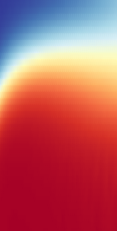
\includegraphics[interpolate=true,width=1.170000in,height=2.310000in]{purity_2qd_heatmap_paper-img0.png}}%
\end{pgfscope}%
\begin{pgfscope}%
\pgfsetbuttcap%
\pgfsetroundjoin%
\definecolor{currentfill}{rgb}{0.000000,0.000000,0.000000}%
\pgfsetfillcolor{currentfill}%
\pgfsetlinewidth{0.803000pt}%
\definecolor{currentstroke}{rgb}{0.000000,0.000000,0.000000}%
\pgfsetstrokecolor{currentstroke}%
\pgfsetdash{}{0pt}%
\pgfsys@defobject{currentmarker}{\pgfqpoint{0.000000in}{-0.048611in}}{\pgfqpoint{0.000000in}{0.000000in}}{%
\pgfpathmoveto{\pgfqpoint{0.000000in}{0.000000in}}%
\pgfpathlineto{\pgfqpoint{0.000000in}{-0.048611in}}%
\pgfusepath{stroke,fill}%
}%
\begin{pgfscope}%
\pgfsys@transformshift{1.042468in}{0.450000in}%
\pgfsys@useobject{currentmarker}{}%
\end{pgfscope}%
\end{pgfscope}%
\begin{pgfscope}%
\definecolor{textcolor}{rgb}{0.000000,0.000000,0.000000}%
\pgfsetstrokecolor{textcolor}%
\pgfsetfillcolor{textcolor}%
\pgftext[x=1.042468in,y=0.352778in,,top]{\color{textcolor}{\rmfamily\fontsize{8.000000}{9.600000}\selectfont\catcode`\^=\active\def^{\ifmmode\sp\else\^{}\fi}\catcode`\%=\active\def%{\%}0.1}}%
\end{pgfscope}%
\begin{pgfscope}%
\pgfsetbuttcap%
\pgfsetroundjoin%
\definecolor{currentfill}{rgb}{0.000000,0.000000,0.000000}%
\pgfsetfillcolor{currentfill}%
\pgfsetlinewidth{0.803000pt}%
\definecolor{currentstroke}{rgb}{0.000000,0.000000,0.000000}%
\pgfsetstrokecolor{currentstroke}%
\pgfsetdash{}{0pt}%
\pgfsys@defobject{currentmarker}{\pgfqpoint{0.000000in}{-0.048611in}}{\pgfqpoint{0.000000in}{0.000000in}}{%
\pgfpathmoveto{\pgfqpoint{0.000000in}{0.000000in}}%
\pgfpathlineto{\pgfqpoint{0.000000in}{-0.048611in}}%
\pgfusepath{stroke,fill}%
}%
\begin{pgfscope}%
\pgfsys@transformshift{1.529915in}{0.450000in}%
\pgfsys@useobject{currentmarker}{}%
\end{pgfscope}%
\end{pgfscope}%
\begin{pgfscope}%
\definecolor{textcolor}{rgb}{0.000000,0.000000,0.000000}%
\pgfsetstrokecolor{textcolor}%
\pgfsetfillcolor{textcolor}%
\pgftext[x=1.529915in,y=0.352778in,,top]{\color{textcolor}{\rmfamily\fontsize{8.000000}{9.600000}\selectfont\catcode`\^=\active\def^{\ifmmode\sp\else\^{}\fi}\catcode`\%=\active\def%{\%}0.2}}%
\end{pgfscope}%
\begin{pgfscope}%
\pgfsetbuttcap%
\pgfsetroundjoin%
\definecolor{currentfill}{rgb}{0.000000,0.000000,0.000000}%
\pgfsetfillcolor{currentfill}%
\pgfsetlinewidth{0.803000pt}%
\definecolor{currentstroke}{rgb}{0.000000,0.000000,0.000000}%
\pgfsetstrokecolor{currentstroke}%
\pgfsetdash{}{0pt}%
\pgfsys@defobject{currentmarker}{\pgfqpoint{-0.048611in}{0.000000in}}{\pgfqpoint{-0.000000in}{0.000000in}}{%
\pgfpathmoveto{\pgfqpoint{-0.000000in}{0.000000in}}%
\pgfpathlineto{\pgfqpoint{-0.048611in}{0.000000in}}%
\pgfusepath{stroke,fill}%
}%
\begin{pgfscope}%
\pgfsys@transformshift{0.750000in}{0.450000in}%
\pgfsys@useobject{currentmarker}{}%
\end{pgfscope}%
\end{pgfscope}%
\begin{pgfscope}%
\definecolor{textcolor}{rgb}{0.000000,0.000000,0.000000}%
\pgfsetstrokecolor{textcolor}%
\pgfsetfillcolor{textcolor}%
\pgftext[x=0.396605in, y=0.410872in, left, base]{\color{textcolor}{\rmfamily\fontsize{8.000000}{9.600000}\selectfont\catcode`\^=\active\def^{\ifmmode\sp\else\^{}\fi}\catcode`\%=\active\def%{\%}$\mathdefault{10^{-3}}$}}%
\end{pgfscope}%
\begin{pgfscope}%
\pgfsetbuttcap%
\pgfsetroundjoin%
\definecolor{currentfill}{rgb}{0.000000,0.000000,0.000000}%
\pgfsetfillcolor{currentfill}%
\pgfsetlinewidth{0.803000pt}%
\definecolor{currentstroke}{rgb}{0.000000,0.000000,0.000000}%
\pgfsetstrokecolor{currentstroke}%
\pgfsetdash{}{0pt}%
\pgfsys@defobject{currentmarker}{\pgfqpoint{-0.048611in}{0.000000in}}{\pgfqpoint{-0.000000in}{0.000000in}}{%
\pgfpathmoveto{\pgfqpoint{-0.000000in}{0.000000in}}%
\pgfpathlineto{\pgfqpoint{-0.048611in}{0.000000in}}%
\pgfusepath{stroke,fill}%
}%
\begin{pgfscope}%
\pgfsys@transformshift{0.750000in}{1.220000in}%
\pgfsys@useobject{currentmarker}{}%
\end{pgfscope}%
\end{pgfscope}%
\begin{pgfscope}%
\definecolor{textcolor}{rgb}{0.000000,0.000000,0.000000}%
\pgfsetstrokecolor{textcolor}%
\pgfsetfillcolor{textcolor}%
\pgftext[x=0.396605in, y=1.180872in, left, base]{\color{textcolor}{\rmfamily\fontsize{8.000000}{9.600000}\selectfont\catcode`\^=\active\def^{\ifmmode\sp\else\^{}\fi}\catcode`\%=\active\def%{\%}$\mathdefault{10^{-2}}$}}%
\end{pgfscope}%
\begin{pgfscope}%
\pgfsetbuttcap%
\pgfsetroundjoin%
\definecolor{currentfill}{rgb}{0.000000,0.000000,0.000000}%
\pgfsetfillcolor{currentfill}%
\pgfsetlinewidth{0.803000pt}%
\definecolor{currentstroke}{rgb}{0.000000,0.000000,0.000000}%
\pgfsetstrokecolor{currentstroke}%
\pgfsetdash{}{0pt}%
\pgfsys@defobject{currentmarker}{\pgfqpoint{-0.048611in}{0.000000in}}{\pgfqpoint{-0.000000in}{0.000000in}}{%
\pgfpathmoveto{\pgfqpoint{-0.000000in}{0.000000in}}%
\pgfpathlineto{\pgfqpoint{-0.048611in}{0.000000in}}%
\pgfusepath{stroke,fill}%
}%
\begin{pgfscope}%
\pgfsys@transformshift{0.750000in}{1.990000in}%
\pgfsys@useobject{currentmarker}{}%
\end{pgfscope}%
\end{pgfscope}%
\begin{pgfscope}%
\definecolor{textcolor}{rgb}{0.000000,0.000000,0.000000}%
\pgfsetstrokecolor{textcolor}%
\pgfsetfillcolor{textcolor}%
\pgftext[x=0.396605in, y=1.950872in, left, base]{\color{textcolor}{\rmfamily\fontsize{8.000000}{9.600000}\selectfont\catcode`\^=\active\def^{\ifmmode\sp\else\^{}\fi}\catcode`\%=\active\def%{\%}$\mathdefault{10^{-1}}$}}%
\end{pgfscope}%
\begin{pgfscope}%
\pgfsetbuttcap%
\pgfsetroundjoin%
\definecolor{currentfill}{rgb}{0.000000,0.000000,0.000000}%
\pgfsetfillcolor{currentfill}%
\pgfsetlinewidth{0.803000pt}%
\definecolor{currentstroke}{rgb}{0.000000,0.000000,0.000000}%
\pgfsetstrokecolor{currentstroke}%
\pgfsetdash{}{0pt}%
\pgfsys@defobject{currentmarker}{\pgfqpoint{-0.048611in}{0.000000in}}{\pgfqpoint{-0.000000in}{0.000000in}}{%
\pgfpathmoveto{\pgfqpoint{-0.000000in}{0.000000in}}%
\pgfpathlineto{\pgfqpoint{-0.048611in}{0.000000in}}%
\pgfusepath{stroke,fill}%
}%
\begin{pgfscope}%
\pgfsys@transformshift{0.750000in}{2.760000in}%
\pgfsys@useobject{currentmarker}{}%
\end{pgfscope}%
\end{pgfscope}%
\begin{pgfscope}%
\definecolor{textcolor}{rgb}{0.000000,0.000000,0.000000}%
\pgfsetstrokecolor{textcolor}%
\pgfsetfillcolor{textcolor}%
\pgftext[x=0.476851in, y=2.720872in, left, base]{\color{textcolor}{\rmfamily\fontsize{8.000000}{9.600000}\selectfont\catcode`\^=\active\def^{\ifmmode\sp\else\^{}\fi}\catcode`\%=\active\def%{\%}$\mathdefault{10^{0}}$}}%
\end{pgfscope}%
\begin{pgfscope}%
\pgfsetbuttcap%
\pgfsetroundjoin%
\definecolor{currentfill}{rgb}{0.000000,0.000000,0.000000}%
\pgfsetfillcolor{currentfill}%
\pgfsetlinewidth{0.602250pt}%
\definecolor{currentstroke}{rgb}{0.000000,0.000000,0.000000}%
\pgfsetstrokecolor{currentstroke}%
\pgfsetdash{}{0pt}%
\pgfsys@defobject{currentmarker}{\pgfqpoint{-0.027778in}{0.000000in}}{\pgfqpoint{-0.000000in}{0.000000in}}{%
\pgfpathmoveto{\pgfqpoint{-0.000000in}{0.000000in}}%
\pgfpathlineto{\pgfqpoint{-0.027778in}{0.000000in}}%
\pgfusepath{stroke,fill}%
}%
\begin{pgfscope}%
\pgfsys@transformshift{0.750000in}{0.681793in}%
\pgfsys@useobject{currentmarker}{}%
\end{pgfscope}%
\end{pgfscope}%
\begin{pgfscope}%
\pgfsetbuttcap%
\pgfsetroundjoin%
\definecolor{currentfill}{rgb}{0.000000,0.000000,0.000000}%
\pgfsetfillcolor{currentfill}%
\pgfsetlinewidth{0.602250pt}%
\definecolor{currentstroke}{rgb}{0.000000,0.000000,0.000000}%
\pgfsetstrokecolor{currentstroke}%
\pgfsetdash{}{0pt}%
\pgfsys@defobject{currentmarker}{\pgfqpoint{-0.027778in}{0.000000in}}{\pgfqpoint{-0.000000in}{0.000000in}}{%
\pgfpathmoveto{\pgfqpoint{-0.000000in}{0.000000in}}%
\pgfpathlineto{\pgfqpoint{-0.027778in}{0.000000in}}%
\pgfusepath{stroke,fill}%
}%
\begin{pgfscope}%
\pgfsys@transformshift{0.750000in}{0.817383in}%
\pgfsys@useobject{currentmarker}{}%
\end{pgfscope}%
\end{pgfscope}%
\begin{pgfscope}%
\pgfsetbuttcap%
\pgfsetroundjoin%
\definecolor{currentfill}{rgb}{0.000000,0.000000,0.000000}%
\pgfsetfillcolor{currentfill}%
\pgfsetlinewidth{0.602250pt}%
\definecolor{currentstroke}{rgb}{0.000000,0.000000,0.000000}%
\pgfsetstrokecolor{currentstroke}%
\pgfsetdash{}{0pt}%
\pgfsys@defobject{currentmarker}{\pgfqpoint{-0.027778in}{0.000000in}}{\pgfqpoint{-0.000000in}{0.000000in}}{%
\pgfpathmoveto{\pgfqpoint{-0.000000in}{0.000000in}}%
\pgfpathlineto{\pgfqpoint{-0.027778in}{0.000000in}}%
\pgfusepath{stroke,fill}%
}%
\begin{pgfscope}%
\pgfsys@transformshift{0.750000in}{0.913586in}%
\pgfsys@useobject{currentmarker}{}%
\end{pgfscope}%
\end{pgfscope}%
\begin{pgfscope}%
\pgfsetbuttcap%
\pgfsetroundjoin%
\definecolor{currentfill}{rgb}{0.000000,0.000000,0.000000}%
\pgfsetfillcolor{currentfill}%
\pgfsetlinewidth{0.602250pt}%
\definecolor{currentstroke}{rgb}{0.000000,0.000000,0.000000}%
\pgfsetstrokecolor{currentstroke}%
\pgfsetdash{}{0pt}%
\pgfsys@defobject{currentmarker}{\pgfqpoint{-0.027778in}{0.000000in}}{\pgfqpoint{-0.000000in}{0.000000in}}{%
\pgfpathmoveto{\pgfqpoint{-0.000000in}{0.000000in}}%
\pgfpathlineto{\pgfqpoint{-0.027778in}{0.000000in}}%
\pgfusepath{stroke,fill}%
}%
\begin{pgfscope}%
\pgfsys@transformshift{0.750000in}{0.988207in}%
\pgfsys@useobject{currentmarker}{}%
\end{pgfscope}%
\end{pgfscope}%
\begin{pgfscope}%
\pgfsetbuttcap%
\pgfsetroundjoin%
\definecolor{currentfill}{rgb}{0.000000,0.000000,0.000000}%
\pgfsetfillcolor{currentfill}%
\pgfsetlinewidth{0.602250pt}%
\definecolor{currentstroke}{rgb}{0.000000,0.000000,0.000000}%
\pgfsetstrokecolor{currentstroke}%
\pgfsetdash{}{0pt}%
\pgfsys@defobject{currentmarker}{\pgfqpoint{-0.027778in}{0.000000in}}{\pgfqpoint{-0.000000in}{0.000000in}}{%
\pgfpathmoveto{\pgfqpoint{-0.000000in}{0.000000in}}%
\pgfpathlineto{\pgfqpoint{-0.027778in}{0.000000in}}%
\pgfusepath{stroke,fill}%
}%
\begin{pgfscope}%
\pgfsys@transformshift{0.750000in}{1.049176in}%
\pgfsys@useobject{currentmarker}{}%
\end{pgfscope}%
\end{pgfscope}%
\begin{pgfscope}%
\pgfsetbuttcap%
\pgfsetroundjoin%
\definecolor{currentfill}{rgb}{0.000000,0.000000,0.000000}%
\pgfsetfillcolor{currentfill}%
\pgfsetlinewidth{0.602250pt}%
\definecolor{currentstroke}{rgb}{0.000000,0.000000,0.000000}%
\pgfsetstrokecolor{currentstroke}%
\pgfsetdash{}{0pt}%
\pgfsys@defobject{currentmarker}{\pgfqpoint{-0.027778in}{0.000000in}}{\pgfqpoint{-0.000000in}{0.000000in}}{%
\pgfpathmoveto{\pgfqpoint{-0.000000in}{0.000000in}}%
\pgfpathlineto{\pgfqpoint{-0.027778in}{0.000000in}}%
\pgfusepath{stroke,fill}%
}%
\begin{pgfscope}%
\pgfsys@transformshift{0.750000in}{1.100725in}%
\pgfsys@useobject{currentmarker}{}%
\end{pgfscope}%
\end{pgfscope}%
\begin{pgfscope}%
\pgfsetbuttcap%
\pgfsetroundjoin%
\definecolor{currentfill}{rgb}{0.000000,0.000000,0.000000}%
\pgfsetfillcolor{currentfill}%
\pgfsetlinewidth{0.602250pt}%
\definecolor{currentstroke}{rgb}{0.000000,0.000000,0.000000}%
\pgfsetstrokecolor{currentstroke}%
\pgfsetdash{}{0pt}%
\pgfsys@defobject{currentmarker}{\pgfqpoint{-0.027778in}{0.000000in}}{\pgfqpoint{-0.000000in}{0.000000in}}{%
\pgfpathmoveto{\pgfqpoint{-0.000000in}{0.000000in}}%
\pgfpathlineto{\pgfqpoint{-0.027778in}{0.000000in}}%
\pgfusepath{stroke,fill}%
}%
\begin{pgfscope}%
\pgfsys@transformshift{0.750000in}{1.145379in}%
\pgfsys@useobject{currentmarker}{}%
\end{pgfscope}%
\end{pgfscope}%
\begin{pgfscope}%
\pgfsetbuttcap%
\pgfsetroundjoin%
\definecolor{currentfill}{rgb}{0.000000,0.000000,0.000000}%
\pgfsetfillcolor{currentfill}%
\pgfsetlinewidth{0.602250pt}%
\definecolor{currentstroke}{rgb}{0.000000,0.000000,0.000000}%
\pgfsetstrokecolor{currentstroke}%
\pgfsetdash{}{0pt}%
\pgfsys@defobject{currentmarker}{\pgfqpoint{-0.027778in}{0.000000in}}{\pgfqpoint{-0.000000in}{0.000000in}}{%
\pgfpathmoveto{\pgfqpoint{-0.000000in}{0.000000in}}%
\pgfpathlineto{\pgfqpoint{-0.027778in}{0.000000in}}%
\pgfusepath{stroke,fill}%
}%
\begin{pgfscope}%
\pgfsys@transformshift{0.750000in}{1.184767in}%
\pgfsys@useobject{currentmarker}{}%
\end{pgfscope}%
\end{pgfscope}%
\begin{pgfscope}%
\pgfsetbuttcap%
\pgfsetroundjoin%
\definecolor{currentfill}{rgb}{0.000000,0.000000,0.000000}%
\pgfsetfillcolor{currentfill}%
\pgfsetlinewidth{0.602250pt}%
\definecolor{currentstroke}{rgb}{0.000000,0.000000,0.000000}%
\pgfsetstrokecolor{currentstroke}%
\pgfsetdash{}{0pt}%
\pgfsys@defobject{currentmarker}{\pgfqpoint{-0.027778in}{0.000000in}}{\pgfqpoint{-0.000000in}{0.000000in}}{%
\pgfpathmoveto{\pgfqpoint{-0.000000in}{0.000000in}}%
\pgfpathlineto{\pgfqpoint{-0.027778in}{0.000000in}}%
\pgfusepath{stroke,fill}%
}%
\begin{pgfscope}%
\pgfsys@transformshift{0.750000in}{1.451793in}%
\pgfsys@useobject{currentmarker}{}%
\end{pgfscope}%
\end{pgfscope}%
\begin{pgfscope}%
\pgfsetbuttcap%
\pgfsetroundjoin%
\definecolor{currentfill}{rgb}{0.000000,0.000000,0.000000}%
\pgfsetfillcolor{currentfill}%
\pgfsetlinewidth{0.602250pt}%
\definecolor{currentstroke}{rgb}{0.000000,0.000000,0.000000}%
\pgfsetstrokecolor{currentstroke}%
\pgfsetdash{}{0pt}%
\pgfsys@defobject{currentmarker}{\pgfqpoint{-0.027778in}{0.000000in}}{\pgfqpoint{-0.000000in}{0.000000in}}{%
\pgfpathmoveto{\pgfqpoint{-0.000000in}{0.000000in}}%
\pgfpathlineto{\pgfqpoint{-0.027778in}{0.000000in}}%
\pgfusepath{stroke,fill}%
}%
\begin{pgfscope}%
\pgfsys@transformshift{0.750000in}{1.587383in}%
\pgfsys@useobject{currentmarker}{}%
\end{pgfscope}%
\end{pgfscope}%
\begin{pgfscope}%
\pgfsetbuttcap%
\pgfsetroundjoin%
\definecolor{currentfill}{rgb}{0.000000,0.000000,0.000000}%
\pgfsetfillcolor{currentfill}%
\pgfsetlinewidth{0.602250pt}%
\definecolor{currentstroke}{rgb}{0.000000,0.000000,0.000000}%
\pgfsetstrokecolor{currentstroke}%
\pgfsetdash{}{0pt}%
\pgfsys@defobject{currentmarker}{\pgfqpoint{-0.027778in}{0.000000in}}{\pgfqpoint{-0.000000in}{0.000000in}}{%
\pgfpathmoveto{\pgfqpoint{-0.000000in}{0.000000in}}%
\pgfpathlineto{\pgfqpoint{-0.027778in}{0.000000in}}%
\pgfusepath{stroke,fill}%
}%
\begin{pgfscope}%
\pgfsys@transformshift{0.750000in}{1.683586in}%
\pgfsys@useobject{currentmarker}{}%
\end{pgfscope}%
\end{pgfscope}%
\begin{pgfscope}%
\pgfsetbuttcap%
\pgfsetroundjoin%
\definecolor{currentfill}{rgb}{0.000000,0.000000,0.000000}%
\pgfsetfillcolor{currentfill}%
\pgfsetlinewidth{0.602250pt}%
\definecolor{currentstroke}{rgb}{0.000000,0.000000,0.000000}%
\pgfsetstrokecolor{currentstroke}%
\pgfsetdash{}{0pt}%
\pgfsys@defobject{currentmarker}{\pgfqpoint{-0.027778in}{0.000000in}}{\pgfqpoint{-0.000000in}{0.000000in}}{%
\pgfpathmoveto{\pgfqpoint{-0.000000in}{0.000000in}}%
\pgfpathlineto{\pgfqpoint{-0.027778in}{0.000000in}}%
\pgfusepath{stroke,fill}%
}%
\begin{pgfscope}%
\pgfsys@transformshift{0.750000in}{1.758207in}%
\pgfsys@useobject{currentmarker}{}%
\end{pgfscope}%
\end{pgfscope}%
\begin{pgfscope}%
\pgfsetbuttcap%
\pgfsetroundjoin%
\definecolor{currentfill}{rgb}{0.000000,0.000000,0.000000}%
\pgfsetfillcolor{currentfill}%
\pgfsetlinewidth{0.602250pt}%
\definecolor{currentstroke}{rgb}{0.000000,0.000000,0.000000}%
\pgfsetstrokecolor{currentstroke}%
\pgfsetdash{}{0pt}%
\pgfsys@defobject{currentmarker}{\pgfqpoint{-0.027778in}{0.000000in}}{\pgfqpoint{-0.000000in}{0.000000in}}{%
\pgfpathmoveto{\pgfqpoint{-0.000000in}{0.000000in}}%
\pgfpathlineto{\pgfqpoint{-0.027778in}{0.000000in}}%
\pgfusepath{stroke,fill}%
}%
\begin{pgfscope}%
\pgfsys@transformshift{0.750000in}{1.819176in}%
\pgfsys@useobject{currentmarker}{}%
\end{pgfscope}%
\end{pgfscope}%
\begin{pgfscope}%
\pgfsetbuttcap%
\pgfsetroundjoin%
\definecolor{currentfill}{rgb}{0.000000,0.000000,0.000000}%
\pgfsetfillcolor{currentfill}%
\pgfsetlinewidth{0.602250pt}%
\definecolor{currentstroke}{rgb}{0.000000,0.000000,0.000000}%
\pgfsetstrokecolor{currentstroke}%
\pgfsetdash{}{0pt}%
\pgfsys@defobject{currentmarker}{\pgfqpoint{-0.027778in}{0.000000in}}{\pgfqpoint{-0.000000in}{0.000000in}}{%
\pgfpathmoveto{\pgfqpoint{-0.000000in}{0.000000in}}%
\pgfpathlineto{\pgfqpoint{-0.027778in}{0.000000in}}%
\pgfusepath{stroke,fill}%
}%
\begin{pgfscope}%
\pgfsys@transformshift{0.750000in}{1.870725in}%
\pgfsys@useobject{currentmarker}{}%
\end{pgfscope}%
\end{pgfscope}%
\begin{pgfscope}%
\pgfsetbuttcap%
\pgfsetroundjoin%
\definecolor{currentfill}{rgb}{0.000000,0.000000,0.000000}%
\pgfsetfillcolor{currentfill}%
\pgfsetlinewidth{0.602250pt}%
\definecolor{currentstroke}{rgb}{0.000000,0.000000,0.000000}%
\pgfsetstrokecolor{currentstroke}%
\pgfsetdash{}{0pt}%
\pgfsys@defobject{currentmarker}{\pgfqpoint{-0.027778in}{0.000000in}}{\pgfqpoint{-0.000000in}{0.000000in}}{%
\pgfpathmoveto{\pgfqpoint{-0.000000in}{0.000000in}}%
\pgfpathlineto{\pgfqpoint{-0.027778in}{0.000000in}}%
\pgfusepath{stroke,fill}%
}%
\begin{pgfscope}%
\pgfsys@transformshift{0.750000in}{1.915379in}%
\pgfsys@useobject{currentmarker}{}%
\end{pgfscope}%
\end{pgfscope}%
\begin{pgfscope}%
\pgfsetbuttcap%
\pgfsetroundjoin%
\definecolor{currentfill}{rgb}{0.000000,0.000000,0.000000}%
\pgfsetfillcolor{currentfill}%
\pgfsetlinewidth{0.602250pt}%
\definecolor{currentstroke}{rgb}{0.000000,0.000000,0.000000}%
\pgfsetstrokecolor{currentstroke}%
\pgfsetdash{}{0pt}%
\pgfsys@defobject{currentmarker}{\pgfqpoint{-0.027778in}{0.000000in}}{\pgfqpoint{-0.000000in}{0.000000in}}{%
\pgfpathmoveto{\pgfqpoint{-0.000000in}{0.000000in}}%
\pgfpathlineto{\pgfqpoint{-0.027778in}{0.000000in}}%
\pgfusepath{stroke,fill}%
}%
\begin{pgfscope}%
\pgfsys@transformshift{0.750000in}{1.954767in}%
\pgfsys@useobject{currentmarker}{}%
\end{pgfscope}%
\end{pgfscope}%
\begin{pgfscope}%
\pgfsetbuttcap%
\pgfsetroundjoin%
\definecolor{currentfill}{rgb}{0.000000,0.000000,0.000000}%
\pgfsetfillcolor{currentfill}%
\pgfsetlinewidth{0.602250pt}%
\definecolor{currentstroke}{rgb}{0.000000,0.000000,0.000000}%
\pgfsetstrokecolor{currentstroke}%
\pgfsetdash{}{0pt}%
\pgfsys@defobject{currentmarker}{\pgfqpoint{-0.027778in}{0.000000in}}{\pgfqpoint{-0.000000in}{0.000000in}}{%
\pgfpathmoveto{\pgfqpoint{-0.000000in}{0.000000in}}%
\pgfpathlineto{\pgfqpoint{-0.027778in}{0.000000in}}%
\pgfusepath{stroke,fill}%
}%
\begin{pgfscope}%
\pgfsys@transformshift{0.750000in}{2.221793in}%
\pgfsys@useobject{currentmarker}{}%
\end{pgfscope}%
\end{pgfscope}%
\begin{pgfscope}%
\pgfsetbuttcap%
\pgfsetroundjoin%
\definecolor{currentfill}{rgb}{0.000000,0.000000,0.000000}%
\pgfsetfillcolor{currentfill}%
\pgfsetlinewidth{0.602250pt}%
\definecolor{currentstroke}{rgb}{0.000000,0.000000,0.000000}%
\pgfsetstrokecolor{currentstroke}%
\pgfsetdash{}{0pt}%
\pgfsys@defobject{currentmarker}{\pgfqpoint{-0.027778in}{0.000000in}}{\pgfqpoint{-0.000000in}{0.000000in}}{%
\pgfpathmoveto{\pgfqpoint{-0.000000in}{0.000000in}}%
\pgfpathlineto{\pgfqpoint{-0.027778in}{0.000000in}}%
\pgfusepath{stroke,fill}%
}%
\begin{pgfscope}%
\pgfsys@transformshift{0.750000in}{2.357383in}%
\pgfsys@useobject{currentmarker}{}%
\end{pgfscope}%
\end{pgfscope}%
\begin{pgfscope}%
\pgfsetbuttcap%
\pgfsetroundjoin%
\definecolor{currentfill}{rgb}{0.000000,0.000000,0.000000}%
\pgfsetfillcolor{currentfill}%
\pgfsetlinewidth{0.602250pt}%
\definecolor{currentstroke}{rgb}{0.000000,0.000000,0.000000}%
\pgfsetstrokecolor{currentstroke}%
\pgfsetdash{}{0pt}%
\pgfsys@defobject{currentmarker}{\pgfqpoint{-0.027778in}{0.000000in}}{\pgfqpoint{-0.000000in}{0.000000in}}{%
\pgfpathmoveto{\pgfqpoint{-0.000000in}{0.000000in}}%
\pgfpathlineto{\pgfqpoint{-0.027778in}{0.000000in}}%
\pgfusepath{stroke,fill}%
}%
\begin{pgfscope}%
\pgfsys@transformshift{0.750000in}{2.453586in}%
\pgfsys@useobject{currentmarker}{}%
\end{pgfscope}%
\end{pgfscope}%
\begin{pgfscope}%
\pgfsetbuttcap%
\pgfsetroundjoin%
\definecolor{currentfill}{rgb}{0.000000,0.000000,0.000000}%
\pgfsetfillcolor{currentfill}%
\pgfsetlinewidth{0.602250pt}%
\definecolor{currentstroke}{rgb}{0.000000,0.000000,0.000000}%
\pgfsetstrokecolor{currentstroke}%
\pgfsetdash{}{0pt}%
\pgfsys@defobject{currentmarker}{\pgfqpoint{-0.027778in}{0.000000in}}{\pgfqpoint{-0.000000in}{0.000000in}}{%
\pgfpathmoveto{\pgfqpoint{-0.000000in}{0.000000in}}%
\pgfpathlineto{\pgfqpoint{-0.027778in}{0.000000in}}%
\pgfusepath{stroke,fill}%
}%
\begin{pgfscope}%
\pgfsys@transformshift{0.750000in}{2.528207in}%
\pgfsys@useobject{currentmarker}{}%
\end{pgfscope}%
\end{pgfscope}%
\begin{pgfscope}%
\pgfsetbuttcap%
\pgfsetroundjoin%
\definecolor{currentfill}{rgb}{0.000000,0.000000,0.000000}%
\pgfsetfillcolor{currentfill}%
\pgfsetlinewidth{0.602250pt}%
\definecolor{currentstroke}{rgb}{0.000000,0.000000,0.000000}%
\pgfsetstrokecolor{currentstroke}%
\pgfsetdash{}{0pt}%
\pgfsys@defobject{currentmarker}{\pgfqpoint{-0.027778in}{0.000000in}}{\pgfqpoint{-0.000000in}{0.000000in}}{%
\pgfpathmoveto{\pgfqpoint{-0.000000in}{0.000000in}}%
\pgfpathlineto{\pgfqpoint{-0.027778in}{0.000000in}}%
\pgfusepath{stroke,fill}%
}%
\begin{pgfscope}%
\pgfsys@transformshift{0.750000in}{2.589176in}%
\pgfsys@useobject{currentmarker}{}%
\end{pgfscope}%
\end{pgfscope}%
\begin{pgfscope}%
\pgfsetbuttcap%
\pgfsetroundjoin%
\definecolor{currentfill}{rgb}{0.000000,0.000000,0.000000}%
\pgfsetfillcolor{currentfill}%
\pgfsetlinewidth{0.602250pt}%
\definecolor{currentstroke}{rgb}{0.000000,0.000000,0.000000}%
\pgfsetstrokecolor{currentstroke}%
\pgfsetdash{}{0pt}%
\pgfsys@defobject{currentmarker}{\pgfqpoint{-0.027778in}{0.000000in}}{\pgfqpoint{-0.000000in}{0.000000in}}{%
\pgfpathmoveto{\pgfqpoint{-0.000000in}{0.000000in}}%
\pgfpathlineto{\pgfqpoint{-0.027778in}{0.000000in}}%
\pgfusepath{stroke,fill}%
}%
\begin{pgfscope}%
\pgfsys@transformshift{0.750000in}{2.640725in}%
\pgfsys@useobject{currentmarker}{}%
\end{pgfscope}%
\end{pgfscope}%
\begin{pgfscope}%
\pgfsetbuttcap%
\pgfsetroundjoin%
\definecolor{currentfill}{rgb}{0.000000,0.000000,0.000000}%
\pgfsetfillcolor{currentfill}%
\pgfsetlinewidth{0.602250pt}%
\definecolor{currentstroke}{rgb}{0.000000,0.000000,0.000000}%
\pgfsetstrokecolor{currentstroke}%
\pgfsetdash{}{0pt}%
\pgfsys@defobject{currentmarker}{\pgfqpoint{-0.027778in}{0.000000in}}{\pgfqpoint{-0.000000in}{0.000000in}}{%
\pgfpathmoveto{\pgfqpoint{-0.000000in}{0.000000in}}%
\pgfpathlineto{\pgfqpoint{-0.027778in}{0.000000in}}%
\pgfusepath{stroke,fill}%
}%
\begin{pgfscope}%
\pgfsys@transformshift{0.750000in}{2.685379in}%
\pgfsys@useobject{currentmarker}{}%
\end{pgfscope}%
\end{pgfscope}%
\begin{pgfscope}%
\pgfsetbuttcap%
\pgfsetroundjoin%
\definecolor{currentfill}{rgb}{0.000000,0.000000,0.000000}%
\pgfsetfillcolor{currentfill}%
\pgfsetlinewidth{0.602250pt}%
\definecolor{currentstroke}{rgb}{0.000000,0.000000,0.000000}%
\pgfsetstrokecolor{currentstroke}%
\pgfsetdash{}{0pt}%
\pgfsys@defobject{currentmarker}{\pgfqpoint{-0.027778in}{0.000000in}}{\pgfqpoint{-0.000000in}{0.000000in}}{%
\pgfpathmoveto{\pgfqpoint{-0.000000in}{0.000000in}}%
\pgfpathlineto{\pgfqpoint{-0.027778in}{0.000000in}}%
\pgfusepath{stroke,fill}%
}%
\begin{pgfscope}%
\pgfsys@transformshift{0.750000in}{2.724767in}%
\pgfsys@useobject{currentmarker}{}%
\end{pgfscope}%
\end{pgfscope}%
\begin{pgfscope}%
\definecolor{textcolor}{rgb}{0.000000,0.000000,0.000000}%
\pgfsetstrokecolor{textcolor}%
\pgfsetfillcolor{textcolor}%
\pgftext[x=0.341049in,y=1.605000in,,bottom,rotate=90.000000]{\color{textcolor}{\rmfamily\fontsize{9.000000}{10.800000}\selectfont\catcode`\^=\active\def^{\ifmmode\sp\else\^{}\fi}\catcode`\%=\active\def%{\%}$\kappa/\omega_b$}}%
\end{pgfscope}%
\begin{pgfscope}%
\pgfsetrectcap%
\pgfsetmiterjoin%
\pgfsetlinewidth{0.803000pt}%
\definecolor{currentstroke}{rgb}{0.000000,0.000000,0.000000}%
\pgfsetstrokecolor{currentstroke}%
\pgfsetdash{}{0pt}%
\pgfpathmoveto{\pgfqpoint{0.750000in}{0.450000in}}%
\pgfpathlineto{\pgfqpoint{0.750000in}{2.760000in}}%
\pgfusepath{stroke}%
\end{pgfscope}%
\begin{pgfscope}%
\pgfsetrectcap%
\pgfsetmiterjoin%
\pgfsetlinewidth{0.803000pt}%
\definecolor{currentstroke}{rgb}{0.000000,0.000000,0.000000}%
\pgfsetstrokecolor{currentstroke}%
\pgfsetdash{}{0pt}%
\pgfpathmoveto{\pgfqpoint{1.919872in}{0.450000in}}%
\pgfpathlineto{\pgfqpoint{1.919872in}{2.760000in}}%
\pgfusepath{stroke}%
\end{pgfscope}%
\begin{pgfscope}%
\pgfsetrectcap%
\pgfsetmiterjoin%
\pgfsetlinewidth{0.803000pt}%
\definecolor{currentstroke}{rgb}{0.000000,0.000000,0.000000}%
\pgfsetstrokecolor{currentstroke}%
\pgfsetdash{}{0pt}%
\pgfpathmoveto{\pgfqpoint{0.750000in}{0.450000in}}%
\pgfpathlineto{\pgfqpoint{1.919872in}{0.450000in}}%
\pgfusepath{stroke}%
\end{pgfscope}%
\begin{pgfscope}%
\pgfsetrectcap%
\pgfsetmiterjoin%
\pgfsetlinewidth{0.803000pt}%
\definecolor{currentstroke}{rgb}{0.000000,0.000000,0.000000}%
\pgfsetstrokecolor{currentstroke}%
\pgfsetdash{}{0pt}%
\pgfpathmoveto{\pgfqpoint{0.750000in}{2.760000in}}%
\pgfpathlineto{\pgfqpoint{1.919872in}{2.760000in}}%
\pgfusepath{stroke}%
\end{pgfscope}%
\begin{pgfscope}%
\definecolor{textcolor}{rgb}{1.000000,1.000000,1.000000}%
\pgfsetstrokecolor{textcolor}%
\pgfsetfillcolor{textcolor}%
\pgftext[x=0.785096in,y=2.713800in,left,top]{\color{textcolor}{\rmfamily\fontsize{9.000000}{10.800000}\selectfont\catcode`\^=\active\def^{\ifmmode\sp\else\^{}\fi}\catcode`\%=\active\def%{\%}$(a)$}}%
\end{pgfscope}%
\begin{pgfscope}%
\definecolor{textcolor}{rgb}{0.200000,0.200000,0.200000}%
\pgfsetstrokecolor{textcolor}%
\pgfsetfillcolor{textcolor}%
\pgftext[x=1.334936in,y=2.829300in,,bottom]{\color{textcolor}{\rmfamily\fontsize{8.000000}{9.600000}\selectfont\catcode`\^=\active\def^{\ifmmode\sp\else\^{}\fi}\catcode`\%=\active\def%{\%}$\prod_{2}$}}%
\end{pgfscope}%
\begin{pgfscope}%
\pgfsetbuttcap%
\pgfsetmiterjoin%
\definecolor{currentfill}{rgb}{1.000000,1.000000,1.000000}%
\pgfsetfillcolor{currentfill}%
\pgfsetlinewidth{0.000000pt}%
\definecolor{currentstroke}{rgb}{0.000000,0.000000,0.000000}%
\pgfsetstrokecolor{currentstroke}%
\pgfsetstrokeopacity{0.000000}%
\pgfsetdash{}{0pt}%
\pgfpathmoveto{\pgfqpoint{1.990064in}{0.450000in}}%
\pgfpathlineto{\pgfqpoint{3.159936in}{0.450000in}}%
\pgfpathlineto{\pgfqpoint{3.159936in}{2.760000in}}%
\pgfpathlineto{\pgfqpoint{1.990064in}{2.760000in}}%
\pgfpathlineto{\pgfqpoint{1.990064in}{0.450000in}}%
\pgfpathclose%
\pgfusepath{fill}%
\end{pgfscope}%
\begin{pgfscope}%
\pgfsys@transformshift{1.990000in}{0.450000in}%
\pgftext[left,bottom]{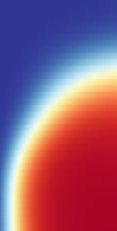
\includegraphics[interpolate=true,width=1.170000in,height=2.310000in]{purity_2qd_heatmap_paper-img1.png}}%
\end{pgfscope}%
\begin{pgfscope}%
\pgfsetbuttcap%
\pgfsetroundjoin%
\definecolor{currentfill}{rgb}{0.000000,0.000000,0.000000}%
\pgfsetfillcolor{currentfill}%
\pgfsetlinewidth{0.803000pt}%
\definecolor{currentstroke}{rgb}{0.000000,0.000000,0.000000}%
\pgfsetstrokecolor{currentstroke}%
\pgfsetdash{}{0pt}%
\pgfsys@defobject{currentmarker}{\pgfqpoint{0.000000in}{-0.048611in}}{\pgfqpoint{0.000000in}{0.000000in}}{%
\pgfpathmoveto{\pgfqpoint{0.000000in}{0.000000in}}%
\pgfpathlineto{\pgfqpoint{0.000000in}{-0.048611in}}%
\pgfusepath{stroke,fill}%
}%
\begin{pgfscope}%
\pgfsys@transformshift{2.282532in}{0.450000in}%
\pgfsys@useobject{currentmarker}{}%
\end{pgfscope}%
\end{pgfscope}%
\begin{pgfscope}%
\definecolor{textcolor}{rgb}{0.000000,0.000000,0.000000}%
\pgfsetstrokecolor{textcolor}%
\pgfsetfillcolor{textcolor}%
\pgftext[x=2.282532in,y=0.352778in,,top]{\color{textcolor}{\rmfamily\fontsize{8.000000}{9.600000}\selectfont\catcode`\^=\active\def^{\ifmmode\sp\else\^{}\fi}\catcode`\%=\active\def%{\%}0.1}}%
\end{pgfscope}%
\begin{pgfscope}%
\pgfsetbuttcap%
\pgfsetroundjoin%
\definecolor{currentfill}{rgb}{0.000000,0.000000,0.000000}%
\pgfsetfillcolor{currentfill}%
\pgfsetlinewidth{0.803000pt}%
\definecolor{currentstroke}{rgb}{0.000000,0.000000,0.000000}%
\pgfsetstrokecolor{currentstroke}%
\pgfsetdash{}{0pt}%
\pgfsys@defobject{currentmarker}{\pgfqpoint{0.000000in}{-0.048611in}}{\pgfqpoint{0.000000in}{0.000000in}}{%
\pgfpathmoveto{\pgfqpoint{0.000000in}{0.000000in}}%
\pgfpathlineto{\pgfqpoint{0.000000in}{-0.048611in}}%
\pgfusepath{stroke,fill}%
}%
\begin{pgfscope}%
\pgfsys@transformshift{2.769979in}{0.450000in}%
\pgfsys@useobject{currentmarker}{}%
\end{pgfscope}%
\end{pgfscope}%
\begin{pgfscope}%
\definecolor{textcolor}{rgb}{0.000000,0.000000,0.000000}%
\pgfsetstrokecolor{textcolor}%
\pgfsetfillcolor{textcolor}%
\pgftext[x=2.769979in,y=0.352778in,,top]{\color{textcolor}{\rmfamily\fontsize{8.000000}{9.600000}\selectfont\catcode`\^=\active\def^{\ifmmode\sp\else\^{}\fi}\catcode`\%=\active\def%{\%}0.2}}%
\end{pgfscope}%
\begin{pgfscope}%
\definecolor{textcolor}{rgb}{0.000000,0.000000,0.000000}%
\pgfsetstrokecolor{textcolor}%
\pgfsetfillcolor{textcolor}%
\pgftext[x=2.575000in,y=0.198457in,,top]{\color{textcolor}{\rmfamily\fontsize{9.000000}{10.800000}\selectfont\catcode`\^=\active\def^{\ifmmode\sp\else\^{}\fi}\catcode`\%=\active\def%{\%}$\lambda/\omega_b$}}%
\end{pgfscope}%
\begin{pgfscope}%
\pgfsetrectcap%
\pgfsetmiterjoin%
\pgfsetlinewidth{0.803000pt}%
\definecolor{currentstroke}{rgb}{0.000000,0.000000,0.000000}%
\pgfsetstrokecolor{currentstroke}%
\pgfsetdash{}{0pt}%
\pgfpathmoveto{\pgfqpoint{1.990064in}{0.450000in}}%
\pgfpathlineto{\pgfqpoint{1.990064in}{2.760000in}}%
\pgfusepath{stroke}%
\end{pgfscope}%
\begin{pgfscope}%
\pgfsetrectcap%
\pgfsetmiterjoin%
\pgfsetlinewidth{0.803000pt}%
\definecolor{currentstroke}{rgb}{0.000000,0.000000,0.000000}%
\pgfsetstrokecolor{currentstroke}%
\pgfsetdash{}{0pt}%
\pgfpathmoveto{\pgfqpoint{3.159936in}{0.450000in}}%
\pgfpathlineto{\pgfqpoint{3.159936in}{2.760000in}}%
\pgfusepath{stroke}%
\end{pgfscope}%
\begin{pgfscope}%
\pgfsetrectcap%
\pgfsetmiterjoin%
\pgfsetlinewidth{0.803000pt}%
\definecolor{currentstroke}{rgb}{0.000000,0.000000,0.000000}%
\pgfsetstrokecolor{currentstroke}%
\pgfsetdash{}{0pt}%
\pgfpathmoveto{\pgfqpoint{1.990064in}{0.450000in}}%
\pgfpathlineto{\pgfqpoint{3.159936in}{0.450000in}}%
\pgfusepath{stroke}%
\end{pgfscope}%
\begin{pgfscope}%
\pgfsetrectcap%
\pgfsetmiterjoin%
\pgfsetlinewidth{0.803000pt}%
\definecolor{currentstroke}{rgb}{0.000000,0.000000,0.000000}%
\pgfsetstrokecolor{currentstroke}%
\pgfsetdash{}{0pt}%
\pgfpathmoveto{\pgfqpoint{1.990064in}{2.760000in}}%
\pgfpathlineto{\pgfqpoint{3.159936in}{2.760000in}}%
\pgfusepath{stroke}%
\end{pgfscope}%
\begin{pgfscope}%
\definecolor{textcolor}{rgb}{1.000000,1.000000,1.000000}%
\pgfsetstrokecolor{textcolor}%
\pgfsetfillcolor{textcolor}%
\pgftext[x=2.025160in,y=2.713800in,left,top]{\color{textcolor}{\rmfamily\fontsize{9.000000}{10.800000}\selectfont\catcode`\^=\active\def^{\ifmmode\sp\else\^{}\fi}\catcode`\%=\active\def%{\%}$(b)$}}%
\end{pgfscope}%
\begin{pgfscope}%
\definecolor{textcolor}{rgb}{0.200000,0.200000,0.200000}%
\pgfsetstrokecolor{textcolor}%
\pgfsetfillcolor{textcolor}%
\pgftext[x=2.575000in,y=2.829300in,,bottom]{\color{textcolor}{\rmfamily\fontsize{8.000000}{9.600000}\selectfont\catcode`\^=\active\def^{\ifmmode\sp\else\^{}\fi}\catcode`\%=\active\def%{\%}$\prod_{3}$}}%
\end{pgfscope}%
\begin{pgfscope}%
\pgfsetbuttcap%
\pgfsetmiterjoin%
\definecolor{currentfill}{rgb}{1.000000,1.000000,1.000000}%
\pgfsetfillcolor{currentfill}%
\pgfsetlinewidth{0.000000pt}%
\definecolor{currentstroke}{rgb}{0.000000,0.000000,0.000000}%
\pgfsetstrokecolor{currentstroke}%
\pgfsetstrokeopacity{0.000000}%
\pgfsetdash{}{0pt}%
\pgfpathmoveto{\pgfqpoint{3.230128in}{0.450000in}}%
\pgfpathlineto{\pgfqpoint{4.400000in}{0.450000in}}%
\pgfpathlineto{\pgfqpoint{4.400000in}{2.760000in}}%
\pgfpathlineto{\pgfqpoint{3.230128in}{2.760000in}}%
\pgfpathlineto{\pgfqpoint{3.230128in}{0.450000in}}%
\pgfpathclose%
\pgfusepath{fill}%
\end{pgfscope}%
\begin{pgfscope}%
\pgfsys@transformshift{3.230000in}{0.450000in}%
\pgftext[left,bottom]{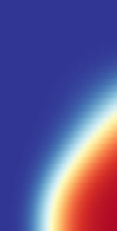
\includegraphics[interpolate=true,width=1.170000in,height=2.310000in]{purity_2qd_heatmap_paper-img2.png}}%
\end{pgfscope}%
\begin{pgfscope}%
\pgfsetbuttcap%
\pgfsetroundjoin%
\definecolor{currentfill}{rgb}{0.000000,0.000000,0.000000}%
\pgfsetfillcolor{currentfill}%
\pgfsetlinewidth{0.803000pt}%
\definecolor{currentstroke}{rgb}{0.000000,0.000000,0.000000}%
\pgfsetstrokecolor{currentstroke}%
\pgfsetdash{}{0pt}%
\pgfsys@defobject{currentmarker}{\pgfqpoint{0.000000in}{-0.048611in}}{\pgfqpoint{0.000000in}{0.000000in}}{%
\pgfpathmoveto{\pgfqpoint{0.000000in}{0.000000in}}%
\pgfpathlineto{\pgfqpoint{0.000000in}{-0.048611in}}%
\pgfusepath{stroke,fill}%
}%
\begin{pgfscope}%
\pgfsys@transformshift{3.522596in}{0.450000in}%
\pgfsys@useobject{currentmarker}{}%
\end{pgfscope}%
\end{pgfscope}%
\begin{pgfscope}%
\definecolor{textcolor}{rgb}{0.000000,0.000000,0.000000}%
\pgfsetstrokecolor{textcolor}%
\pgfsetfillcolor{textcolor}%
\pgftext[x=3.522596in,y=0.352778in,,top]{\color{textcolor}{\rmfamily\fontsize{8.000000}{9.600000}\selectfont\catcode`\^=\active\def^{\ifmmode\sp\else\^{}\fi}\catcode`\%=\active\def%{\%}0.1}}%
\end{pgfscope}%
\begin{pgfscope}%
\pgfsetbuttcap%
\pgfsetroundjoin%
\definecolor{currentfill}{rgb}{0.000000,0.000000,0.000000}%
\pgfsetfillcolor{currentfill}%
\pgfsetlinewidth{0.803000pt}%
\definecolor{currentstroke}{rgb}{0.000000,0.000000,0.000000}%
\pgfsetstrokecolor{currentstroke}%
\pgfsetdash{}{0pt}%
\pgfsys@defobject{currentmarker}{\pgfqpoint{0.000000in}{-0.048611in}}{\pgfqpoint{0.000000in}{0.000000in}}{%
\pgfpathmoveto{\pgfqpoint{0.000000in}{0.000000in}}%
\pgfpathlineto{\pgfqpoint{0.000000in}{-0.048611in}}%
\pgfusepath{stroke,fill}%
}%
\begin{pgfscope}%
\pgfsys@transformshift{4.010043in}{0.450000in}%
\pgfsys@useobject{currentmarker}{}%
\end{pgfscope}%
\end{pgfscope}%
\begin{pgfscope}%
\definecolor{textcolor}{rgb}{0.000000,0.000000,0.000000}%
\pgfsetstrokecolor{textcolor}%
\pgfsetfillcolor{textcolor}%
\pgftext[x=4.010043in,y=0.352778in,,top]{\color{textcolor}{\rmfamily\fontsize{8.000000}{9.600000}\selectfont\catcode`\^=\active\def^{\ifmmode\sp\else\^{}\fi}\catcode`\%=\active\def%{\%}0.2}}%
\end{pgfscope}%
\begin{pgfscope}%
\pgfsetrectcap%
\pgfsetmiterjoin%
\pgfsetlinewidth{0.803000pt}%
\definecolor{currentstroke}{rgb}{0.000000,0.000000,0.000000}%
\pgfsetstrokecolor{currentstroke}%
\pgfsetdash{}{0pt}%
\pgfpathmoveto{\pgfqpoint{3.230128in}{0.450000in}}%
\pgfpathlineto{\pgfqpoint{3.230128in}{2.760000in}}%
\pgfusepath{stroke}%
\end{pgfscope}%
\begin{pgfscope}%
\pgfsetrectcap%
\pgfsetmiterjoin%
\pgfsetlinewidth{0.803000pt}%
\definecolor{currentstroke}{rgb}{0.000000,0.000000,0.000000}%
\pgfsetstrokecolor{currentstroke}%
\pgfsetdash{}{0pt}%
\pgfpathmoveto{\pgfqpoint{4.400000in}{0.450000in}}%
\pgfpathlineto{\pgfqpoint{4.400000in}{2.760000in}}%
\pgfusepath{stroke}%
\end{pgfscope}%
\begin{pgfscope}%
\pgfsetrectcap%
\pgfsetmiterjoin%
\pgfsetlinewidth{0.803000pt}%
\definecolor{currentstroke}{rgb}{0.000000,0.000000,0.000000}%
\pgfsetstrokecolor{currentstroke}%
\pgfsetdash{}{0pt}%
\pgfpathmoveto{\pgfqpoint{3.230128in}{0.450000in}}%
\pgfpathlineto{\pgfqpoint{4.400000in}{0.450000in}}%
\pgfusepath{stroke}%
\end{pgfscope}%
\begin{pgfscope}%
\pgfsetrectcap%
\pgfsetmiterjoin%
\pgfsetlinewidth{0.803000pt}%
\definecolor{currentstroke}{rgb}{0.000000,0.000000,0.000000}%
\pgfsetstrokecolor{currentstroke}%
\pgfsetdash{}{0pt}%
\pgfpathmoveto{\pgfqpoint{3.230128in}{2.760000in}}%
\pgfpathlineto{\pgfqpoint{4.400000in}{2.760000in}}%
\pgfusepath{stroke}%
\end{pgfscope}%
\begin{pgfscope}%
\definecolor{textcolor}{rgb}{1.000000,1.000000,1.000000}%
\pgfsetstrokecolor{textcolor}%
\pgfsetfillcolor{textcolor}%
\pgftext[x=3.265224in,y=2.713800in,left,top]{\color{textcolor}{\rmfamily\fontsize{9.000000}{10.800000}\selectfont\catcode`\^=\active\def^{\ifmmode\sp\else\^{}\fi}\catcode`\%=\active\def%{\%}$(c)$}}%
\end{pgfscope}%
\begin{pgfscope}%
\definecolor{textcolor}{rgb}{0.200000,0.200000,0.200000}%
\pgfsetstrokecolor{textcolor}%
\pgfsetfillcolor{textcolor}%
\pgftext[x=3.815064in,y=2.829300in,,bottom]{\color{textcolor}{\rmfamily\fontsize{8.000000}{9.600000}\selectfont\catcode`\^=\active\def^{\ifmmode\sp\else\^{}\fi}\catcode`\%=\active\def%{\%}$\prod_{4}$}}%
\end{pgfscope}%
\begin{pgfscope}%
\pgfsetbuttcap%
\pgfsetmiterjoin%
\definecolor{currentfill}{rgb}{1.000000,1.000000,1.000000}%
\pgfsetfillcolor{currentfill}%
\pgfsetlinewidth{0.000000pt}%
\definecolor{currentstroke}{rgb}{0.000000,0.000000,0.000000}%
\pgfsetstrokecolor{currentstroke}%
\pgfsetstrokeopacity{0.000000}%
\pgfsetdash{}{0pt}%
\pgfpathmoveto{\pgfqpoint{4.500000in}{0.450000in}}%
\pgfpathlineto{\pgfqpoint{4.600000in}{0.450000in}}%
\pgfpathlineto{\pgfqpoint{4.600000in}{2.760000in}}%
\pgfpathlineto{\pgfqpoint{4.500000in}{2.760000in}}%
\pgfpathlineto{\pgfqpoint{4.500000in}{0.450000in}}%
\pgfpathclose%
\pgfusepath{fill}%
\end{pgfscope}%
\begin{pgfscope}%
\pgfsys@transformshift{4.500000in}{0.450000in}%
\pgftext[left,bottom]{
\includegraphics[interpolate=true,width=0.100000in,height=2.310000in]{purity_2qd_heatmap_paper-img3.png}}%
\end{pgfscope}%
\begin{pgfscope}%
\pgfsetbuttcap%
\pgfsetroundjoin%
\definecolor{currentfill}{rgb}{0.000000,0.000000,0.000000}%
\pgfsetfillcolor{currentfill}%
\pgfsetlinewidth{0.803000pt}%
\definecolor{currentstroke}{rgb}{0.000000,0.000000,0.000000}%
\pgfsetstrokecolor{currentstroke}%
\pgfsetdash{}{0pt}%
\pgfsys@defobject{currentmarker}{\pgfqpoint{0.000000in}{0.000000in}}{\pgfqpoint{0.048611in}{0.000000in}}{%
\pgfpathmoveto{\pgfqpoint{0.000000in}{0.000000in}}%
\pgfpathlineto{\pgfqpoint{0.048611in}{0.000000in}}%
\pgfusepath{stroke,fill}%
}%
\begin{pgfscope}%
\pgfsys@transformshift{4.600000in}{0.450000in}%
\pgfsys@useobject{currentmarker}{}%
\end{pgfscope}%
\end{pgfscope}%
\begin{pgfscope}%
\definecolor{textcolor}{rgb}{0.000000,0.000000,0.000000}%
\pgfsetstrokecolor{textcolor}%
\pgfsetfillcolor{textcolor}%
\pgftext[x=4.697222in, y=0.411420in, left, base]{\color{textcolor}{\rmfamily\fontsize{8.000000}{9.600000}\selectfont\catcode`\^=\active\def^{\ifmmode\sp\else\^{}\fi}\catcode`\%=\active\def%{\%}0.0}}%
\end{pgfscope}%
\begin{pgfscope}%
\pgfsetbuttcap%
\pgfsetroundjoin%
\definecolor{currentfill}{rgb}{0.000000,0.000000,0.000000}%
\pgfsetfillcolor{currentfill}%
\pgfsetlinewidth{0.803000pt}%
\definecolor{currentstroke}{rgb}{0.000000,0.000000,0.000000}%
\pgfsetstrokecolor{currentstroke}%
\pgfsetdash{}{0pt}%
\pgfsys@defobject{currentmarker}{\pgfqpoint{0.000000in}{0.000000in}}{\pgfqpoint{0.048611in}{0.000000in}}{%
\pgfpathmoveto{\pgfqpoint{0.000000in}{0.000000in}}%
\pgfpathlineto{\pgfqpoint{0.048611in}{0.000000in}}%
\pgfusepath{stroke,fill}%
}%
\begin{pgfscope}%
\pgfsys@transformshift{4.600000in}{1.605000in}%
\pgfsys@useobject{currentmarker}{}%
\end{pgfscope}%
\end{pgfscope}%
\begin{pgfscope}%
\definecolor{textcolor}{rgb}{0.000000,0.000000,0.000000}%
\pgfsetstrokecolor{textcolor}%
\pgfsetfillcolor{textcolor}%
\pgftext[x=4.697222in, y=1.566420in, left, base]{\color{textcolor}{\rmfamily\fontsize{8.000000}{9.600000}\selectfont\catcode`\^=\active\def^{\ifmmode\sp\else\^{}\fi}\catcode`\%=\active\def%{\%}0.5}}%
\end{pgfscope}%
\begin{pgfscope}%
\pgfsetbuttcap%
\pgfsetroundjoin%
\definecolor{currentfill}{rgb}{0.000000,0.000000,0.000000}%
\pgfsetfillcolor{currentfill}%
\pgfsetlinewidth{0.803000pt}%
\definecolor{currentstroke}{rgb}{0.000000,0.000000,0.000000}%
\pgfsetstrokecolor{currentstroke}%
\pgfsetdash{}{0pt}%
\pgfsys@defobject{currentmarker}{\pgfqpoint{0.000000in}{0.000000in}}{\pgfqpoint{0.048611in}{0.000000in}}{%
\pgfpathmoveto{\pgfqpoint{0.000000in}{0.000000in}}%
\pgfpathlineto{\pgfqpoint{0.048611in}{0.000000in}}%
\pgfusepath{stroke,fill}%
}%
\begin{pgfscope}%
\pgfsys@transformshift{4.600000in}{2.760000in}%
\pgfsys@useobject{currentmarker}{}%
\end{pgfscope}%
\end{pgfscope}%
\begin{pgfscope}%
\definecolor{textcolor}{rgb}{0.000000,0.000000,0.000000}%
\pgfsetstrokecolor{textcolor}%
\pgfsetfillcolor{textcolor}%
\pgftext[x=4.697222in, y=2.721420in, left, base]{\color{textcolor}{\rmfamily\fontsize{8.000000}{9.600000}\selectfont\catcode`\^=\active\def^{\ifmmode\sp\else\^{}\fi}\catcode`\%=\active\def%{\%}1.0}}%
\end{pgfscope}%
\begin{pgfscope}%
\pgfsetrectcap%
\pgfsetmiterjoin%
\pgfsetlinewidth{0.803000pt}%
\definecolor{currentstroke}{rgb}{0.000000,0.000000,0.000000}%
\pgfsetstrokecolor{currentstroke}%
\pgfsetdash{}{0pt}%
\pgfpathmoveto{\pgfqpoint{4.500000in}{0.450000in}}%
\pgfpathlineto{\pgfqpoint{4.550000in}{0.450000in}}%
\pgfpathlineto{\pgfqpoint{4.600000in}{0.450000in}}%
\pgfpathlineto{\pgfqpoint{4.600000in}{2.760000in}}%
\pgfpathlineto{\pgfqpoint{4.550000in}{2.760000in}}%
\pgfpathlineto{\pgfqpoint{4.500000in}{2.760000in}}%
\pgfpathlineto{\pgfqpoint{4.500000in}{0.450000in}}%
\pgfpathclose%
\pgfusepath{stroke}%
\end{pgfscope}%
\end{pgfpicture}%
\makeatother%
\endgroup%

	\caption{Mapas de pureza $\Pi_n$ para $n = 2, 3, 4$ (de izquierda a
		derecha) en función de $\lambda/\omega_b$ y $\kappa/\omega_b$,
		evaluados en la condición de resonancia de Stokes de orden $n$. Parámetros: $\Omega/\omega_b = 0.2$,
		$\gamma/\omega_b = 0.0002$, $\gamma_\varphi/\omega_b = 0.0004$,
		$J/\omega_b = 0.5$.}
	\label{fig:purity_2qd_heatmap}
\end{figure}

\newpage
\begin{figure}[H]
	\centering
	%% Creator: Matplotlib, PGF backend
%%
%% To include the figure in your LaTeX document, write
%%   \input{<filename>.pgf}
%%
%% Make sure the required packages are loaded in your preamble
%%   \usepackage{pgf}
%%
%% Also ensure that all the required font packages are loaded; for instance,
%% the lmodern package is sometimes necessary when using math font.
%%   \usepackage{lmodern}
%%
%% Figures using additional raster images can only be included by \input if
%% they are in the same directory as the main LaTeX file. For loading figures
%% from other directories you can use the `import` package
%%   \usepackage{import}
%%
%% and then include the figures with
%%   \import{<path to file>}{<filename>.pgf}
%%
%% Matplotlib used the following preamble
%%   \def\mathdefault#1{#1}
%%   \everymath=\expandafter{\the\everymath\displaystyle}
%%   \IfFileExists{scrextend.sty}{
%%     \usepackage[fontsize=8.000000pt]{scrextend}
%%   }{
%%     \renewcommand{\normalsize}{\fontsize{8.000000}{9.600000}\selectfont}
%%     \normalsize
%%   }
%%   
%%   \makeatletter\@ifpackageloaded{underscore}{}{\usepackage[strings]{underscore}}\makeatother
%%
\begingroup%
\makeatletter%
\begin{pgfpicture}%
\pgfpathrectangle{\pgfpointorigin}{\pgfqpoint{5.100000in}{2.200000in}}%
\pgfusepath{use as bounding box, clip}%
\begin{pgfscope}%
\pgfsetbuttcap%
\pgfsetmiterjoin%
\definecolor{currentfill}{rgb}{1.000000,1.000000,1.000000}%
\pgfsetfillcolor{currentfill}%
\pgfsetlinewidth{0.000000pt}%
\definecolor{currentstroke}{rgb}{1.000000,1.000000,1.000000}%
\pgfsetstrokecolor{currentstroke}%
\pgfsetdash{}{0pt}%
\pgfpathmoveto{\pgfqpoint{0.000000in}{0.000000in}}%
\pgfpathlineto{\pgfqpoint{5.100000in}{0.000000in}}%
\pgfpathlineto{\pgfqpoint{5.100000in}{2.200000in}}%
\pgfpathlineto{\pgfqpoint{0.000000in}{2.200000in}}%
\pgfpathlineto{\pgfqpoint{0.000000in}{0.000000in}}%
\pgfpathclose%
\pgfusepath{fill}%
\end{pgfscope}%
\begin{pgfscope}%
\pgfsetbuttcap%
\pgfsetmiterjoin%
\definecolor{currentfill}{rgb}{1.000000,1.000000,1.000000}%
\pgfsetfillcolor{currentfill}%
\pgfsetlinewidth{0.000000pt}%
\definecolor{currentstroke}{rgb}{0.000000,0.000000,0.000000}%
\pgfsetstrokecolor{currentstroke}%
\pgfsetstrokeopacity{0.000000}%
\pgfsetdash{}{0pt}%
\pgfpathmoveto{\pgfqpoint{0.510000in}{0.484000in}}%
\pgfpathlineto{\pgfqpoint{2.554811in}{0.484000in}}%
\pgfpathlineto{\pgfqpoint{2.554811in}{1.936000in}}%
\pgfpathlineto{\pgfqpoint{0.510000in}{1.936000in}}%
\pgfpathlineto{\pgfqpoint{0.510000in}{0.484000in}}%
\pgfpathclose%
\pgfusepath{fill}%
\end{pgfscope}%
\begin{pgfscope}%
\pgfsetbuttcap%
\pgfsetroundjoin%
\definecolor{currentfill}{rgb}{0.000000,0.000000,0.000000}%
\pgfsetfillcolor{currentfill}%
\pgfsetlinewidth{0.803000pt}%
\definecolor{currentstroke}{rgb}{0.000000,0.000000,0.000000}%
\pgfsetstrokecolor{currentstroke}%
\pgfsetdash{}{0pt}%
\pgfsys@defobject{currentmarker}{\pgfqpoint{0.000000in}{-0.048611in}}{\pgfqpoint{0.000000in}{0.000000in}}{%
\pgfpathmoveto{\pgfqpoint{0.000000in}{0.000000in}}%
\pgfpathlineto{\pgfqpoint{0.000000in}{-0.048611in}}%
\pgfusepath{stroke,fill}%
}%
\begin{pgfscope}%
\pgfsys@transformshift{0.510000in}{0.484000in}%
\pgfsys@useobject{currentmarker}{}%
\end{pgfscope}%
\end{pgfscope}%
\begin{pgfscope}%
\definecolor{textcolor}{rgb}{0.000000,0.000000,0.000000}%
\pgfsetstrokecolor{textcolor}%
\pgfsetfillcolor{textcolor}%
\pgftext[x=0.510000in,y=0.386778in,,top]{\color{textcolor}{\rmfamily\fontsize{8.000000}{9.600000}\selectfont\catcode`\^=\active\def^{\ifmmode\sp\else\^{}\fi}\catcode`\%=\active\def%{\%}$\mathdefault{10^{-3}}$}}%
\end{pgfscope}%
\begin{pgfscope}%
\pgfsetbuttcap%
\pgfsetroundjoin%
\definecolor{currentfill}{rgb}{0.000000,0.000000,0.000000}%
\pgfsetfillcolor{currentfill}%
\pgfsetlinewidth{0.803000pt}%
\definecolor{currentstroke}{rgb}{0.000000,0.000000,0.000000}%
\pgfsetstrokecolor{currentstroke}%
\pgfsetdash{}{0pt}%
\pgfsys@defobject{currentmarker}{\pgfqpoint{0.000000in}{-0.048611in}}{\pgfqpoint{0.000000in}{0.000000in}}{%
\pgfpathmoveto{\pgfqpoint{0.000000in}{0.000000in}}%
\pgfpathlineto{\pgfqpoint{0.000000in}{-0.048611in}}%
\pgfusepath{stroke,fill}%
}%
\begin{pgfscope}%
\pgfsys@transformshift{1.191604in}{0.484000in}%
\pgfsys@useobject{currentmarker}{}%
\end{pgfscope}%
\end{pgfscope}%
\begin{pgfscope}%
\definecolor{textcolor}{rgb}{0.000000,0.000000,0.000000}%
\pgfsetstrokecolor{textcolor}%
\pgfsetfillcolor{textcolor}%
\pgftext[x=1.191604in,y=0.386778in,,top]{\color{textcolor}{\rmfamily\fontsize{8.000000}{9.600000}\selectfont\catcode`\^=\active\def^{\ifmmode\sp\else\^{}\fi}\catcode`\%=\active\def%{\%}$\mathdefault{10^{-2}}$}}%
\end{pgfscope}%
\begin{pgfscope}%
\pgfsetbuttcap%
\pgfsetroundjoin%
\definecolor{currentfill}{rgb}{0.000000,0.000000,0.000000}%
\pgfsetfillcolor{currentfill}%
\pgfsetlinewidth{0.803000pt}%
\definecolor{currentstroke}{rgb}{0.000000,0.000000,0.000000}%
\pgfsetstrokecolor{currentstroke}%
\pgfsetdash{}{0pt}%
\pgfsys@defobject{currentmarker}{\pgfqpoint{0.000000in}{-0.048611in}}{\pgfqpoint{0.000000in}{0.000000in}}{%
\pgfpathmoveto{\pgfqpoint{0.000000in}{0.000000in}}%
\pgfpathlineto{\pgfqpoint{0.000000in}{-0.048611in}}%
\pgfusepath{stroke,fill}%
}%
\begin{pgfscope}%
\pgfsys@transformshift{1.873208in}{0.484000in}%
\pgfsys@useobject{currentmarker}{}%
\end{pgfscope}%
\end{pgfscope}%
\begin{pgfscope}%
\definecolor{textcolor}{rgb}{0.000000,0.000000,0.000000}%
\pgfsetstrokecolor{textcolor}%
\pgfsetfillcolor{textcolor}%
\pgftext[x=1.873208in,y=0.386778in,,top]{\color{textcolor}{\rmfamily\fontsize{8.000000}{9.600000}\selectfont\catcode`\^=\active\def^{\ifmmode\sp\else\^{}\fi}\catcode`\%=\active\def%{\%}$\mathdefault{10^{-1}}$}}%
\end{pgfscope}%
\begin{pgfscope}%
\pgfsetbuttcap%
\pgfsetroundjoin%
\definecolor{currentfill}{rgb}{0.000000,0.000000,0.000000}%
\pgfsetfillcolor{currentfill}%
\pgfsetlinewidth{0.803000pt}%
\definecolor{currentstroke}{rgb}{0.000000,0.000000,0.000000}%
\pgfsetstrokecolor{currentstroke}%
\pgfsetdash{}{0pt}%
\pgfsys@defobject{currentmarker}{\pgfqpoint{0.000000in}{-0.048611in}}{\pgfqpoint{0.000000in}{0.000000in}}{%
\pgfpathmoveto{\pgfqpoint{0.000000in}{0.000000in}}%
\pgfpathlineto{\pgfqpoint{0.000000in}{-0.048611in}}%
\pgfusepath{stroke,fill}%
}%
\begin{pgfscope}%
\pgfsys@transformshift{2.554811in}{0.484000in}%
\pgfsys@useobject{currentmarker}{}%
\end{pgfscope}%
\end{pgfscope}%
\begin{pgfscope}%
\definecolor{textcolor}{rgb}{0.000000,0.000000,0.000000}%
\pgfsetstrokecolor{textcolor}%
\pgfsetfillcolor{textcolor}%
\pgftext[x=2.554811in,y=0.386778in,,top]{\color{textcolor}{\rmfamily\fontsize{8.000000}{9.600000}\selectfont\catcode`\^=\active\def^{\ifmmode\sp\else\^{}\fi}\catcode`\%=\active\def%{\%}$\mathdefault{10^{0}}$}}%
\end{pgfscope}%
\begin{pgfscope}%
\pgfsetbuttcap%
\pgfsetroundjoin%
\definecolor{currentfill}{rgb}{0.000000,0.000000,0.000000}%
\pgfsetfillcolor{currentfill}%
\pgfsetlinewidth{0.602250pt}%
\definecolor{currentstroke}{rgb}{0.000000,0.000000,0.000000}%
\pgfsetstrokecolor{currentstroke}%
\pgfsetdash{}{0pt}%
\pgfsys@defobject{currentmarker}{\pgfqpoint{0.000000in}{-0.027778in}}{\pgfqpoint{0.000000in}{0.000000in}}{%
\pgfpathmoveto{\pgfqpoint{0.000000in}{0.000000in}}%
\pgfpathlineto{\pgfqpoint{0.000000in}{-0.027778in}}%
\pgfusepath{stroke,fill}%
}%
\begin{pgfscope}%
\pgfsys@transformshift{0.715183in}{0.484000in}%
\pgfsys@useobject{currentmarker}{}%
\end{pgfscope}%
\end{pgfscope}%
\begin{pgfscope}%
\pgfsetbuttcap%
\pgfsetroundjoin%
\definecolor{currentfill}{rgb}{0.000000,0.000000,0.000000}%
\pgfsetfillcolor{currentfill}%
\pgfsetlinewidth{0.602250pt}%
\definecolor{currentstroke}{rgb}{0.000000,0.000000,0.000000}%
\pgfsetstrokecolor{currentstroke}%
\pgfsetdash{}{0pt}%
\pgfsys@defobject{currentmarker}{\pgfqpoint{0.000000in}{-0.027778in}}{\pgfqpoint{0.000000in}{0.000000in}}{%
\pgfpathmoveto{\pgfqpoint{0.000000in}{0.000000in}}%
\pgfpathlineto{\pgfqpoint{0.000000in}{-0.027778in}}%
\pgfusepath{stroke,fill}%
}%
\begin{pgfscope}%
\pgfsys@transformshift{0.835208in}{0.484000in}%
\pgfsys@useobject{currentmarker}{}%
\end{pgfscope}%
\end{pgfscope}%
\begin{pgfscope}%
\pgfsetbuttcap%
\pgfsetroundjoin%
\definecolor{currentfill}{rgb}{0.000000,0.000000,0.000000}%
\pgfsetfillcolor{currentfill}%
\pgfsetlinewidth{0.602250pt}%
\definecolor{currentstroke}{rgb}{0.000000,0.000000,0.000000}%
\pgfsetstrokecolor{currentstroke}%
\pgfsetdash{}{0pt}%
\pgfsys@defobject{currentmarker}{\pgfqpoint{0.000000in}{-0.027778in}}{\pgfqpoint{0.000000in}{0.000000in}}{%
\pgfpathmoveto{\pgfqpoint{0.000000in}{0.000000in}}%
\pgfpathlineto{\pgfqpoint{0.000000in}{-0.027778in}}%
\pgfusepath{stroke,fill}%
}%
\begin{pgfscope}%
\pgfsys@transformshift{0.920366in}{0.484000in}%
\pgfsys@useobject{currentmarker}{}%
\end{pgfscope}%
\end{pgfscope}%
\begin{pgfscope}%
\pgfsetbuttcap%
\pgfsetroundjoin%
\definecolor{currentfill}{rgb}{0.000000,0.000000,0.000000}%
\pgfsetfillcolor{currentfill}%
\pgfsetlinewidth{0.602250pt}%
\definecolor{currentstroke}{rgb}{0.000000,0.000000,0.000000}%
\pgfsetstrokecolor{currentstroke}%
\pgfsetdash{}{0pt}%
\pgfsys@defobject{currentmarker}{\pgfqpoint{0.000000in}{-0.027778in}}{\pgfqpoint{0.000000in}{0.000000in}}{%
\pgfpathmoveto{\pgfqpoint{0.000000in}{0.000000in}}%
\pgfpathlineto{\pgfqpoint{0.000000in}{-0.027778in}}%
\pgfusepath{stroke,fill}%
}%
\begin{pgfscope}%
\pgfsys@transformshift{0.986421in}{0.484000in}%
\pgfsys@useobject{currentmarker}{}%
\end{pgfscope}%
\end{pgfscope}%
\begin{pgfscope}%
\pgfsetbuttcap%
\pgfsetroundjoin%
\definecolor{currentfill}{rgb}{0.000000,0.000000,0.000000}%
\pgfsetfillcolor{currentfill}%
\pgfsetlinewidth{0.602250pt}%
\definecolor{currentstroke}{rgb}{0.000000,0.000000,0.000000}%
\pgfsetstrokecolor{currentstroke}%
\pgfsetdash{}{0pt}%
\pgfsys@defobject{currentmarker}{\pgfqpoint{0.000000in}{-0.027778in}}{\pgfqpoint{0.000000in}{0.000000in}}{%
\pgfpathmoveto{\pgfqpoint{0.000000in}{0.000000in}}%
\pgfpathlineto{\pgfqpoint{0.000000in}{-0.027778in}}%
\pgfusepath{stroke,fill}%
}%
\begin{pgfscope}%
\pgfsys@transformshift{1.040391in}{0.484000in}%
\pgfsys@useobject{currentmarker}{}%
\end{pgfscope}%
\end{pgfscope}%
\begin{pgfscope}%
\pgfsetbuttcap%
\pgfsetroundjoin%
\definecolor{currentfill}{rgb}{0.000000,0.000000,0.000000}%
\pgfsetfillcolor{currentfill}%
\pgfsetlinewidth{0.602250pt}%
\definecolor{currentstroke}{rgb}{0.000000,0.000000,0.000000}%
\pgfsetstrokecolor{currentstroke}%
\pgfsetdash{}{0pt}%
\pgfsys@defobject{currentmarker}{\pgfqpoint{0.000000in}{-0.027778in}}{\pgfqpoint{0.000000in}{0.000000in}}{%
\pgfpathmoveto{\pgfqpoint{0.000000in}{0.000000in}}%
\pgfpathlineto{\pgfqpoint{0.000000in}{-0.027778in}}%
\pgfusepath{stroke,fill}%
}%
\begin{pgfscope}%
\pgfsys@transformshift{1.086022in}{0.484000in}%
\pgfsys@useobject{currentmarker}{}%
\end{pgfscope}%
\end{pgfscope}%
\begin{pgfscope}%
\pgfsetbuttcap%
\pgfsetroundjoin%
\definecolor{currentfill}{rgb}{0.000000,0.000000,0.000000}%
\pgfsetfillcolor{currentfill}%
\pgfsetlinewidth{0.602250pt}%
\definecolor{currentstroke}{rgb}{0.000000,0.000000,0.000000}%
\pgfsetstrokecolor{currentstroke}%
\pgfsetdash{}{0pt}%
\pgfsys@defobject{currentmarker}{\pgfqpoint{0.000000in}{-0.027778in}}{\pgfqpoint{0.000000in}{0.000000in}}{%
\pgfpathmoveto{\pgfqpoint{0.000000in}{0.000000in}}%
\pgfpathlineto{\pgfqpoint{0.000000in}{-0.027778in}}%
\pgfusepath{stroke,fill}%
}%
\begin{pgfscope}%
\pgfsys@transformshift{1.125550in}{0.484000in}%
\pgfsys@useobject{currentmarker}{}%
\end{pgfscope}%
\end{pgfscope}%
\begin{pgfscope}%
\pgfsetbuttcap%
\pgfsetroundjoin%
\definecolor{currentfill}{rgb}{0.000000,0.000000,0.000000}%
\pgfsetfillcolor{currentfill}%
\pgfsetlinewidth{0.602250pt}%
\definecolor{currentstroke}{rgb}{0.000000,0.000000,0.000000}%
\pgfsetstrokecolor{currentstroke}%
\pgfsetdash{}{0pt}%
\pgfsys@defobject{currentmarker}{\pgfqpoint{0.000000in}{-0.027778in}}{\pgfqpoint{0.000000in}{0.000000in}}{%
\pgfpathmoveto{\pgfqpoint{0.000000in}{0.000000in}}%
\pgfpathlineto{\pgfqpoint{0.000000in}{-0.027778in}}%
\pgfusepath{stroke,fill}%
}%
\begin{pgfscope}%
\pgfsys@transformshift{1.160415in}{0.484000in}%
\pgfsys@useobject{currentmarker}{}%
\end{pgfscope}%
\end{pgfscope}%
\begin{pgfscope}%
\pgfsetbuttcap%
\pgfsetroundjoin%
\definecolor{currentfill}{rgb}{0.000000,0.000000,0.000000}%
\pgfsetfillcolor{currentfill}%
\pgfsetlinewidth{0.602250pt}%
\definecolor{currentstroke}{rgb}{0.000000,0.000000,0.000000}%
\pgfsetstrokecolor{currentstroke}%
\pgfsetdash{}{0pt}%
\pgfsys@defobject{currentmarker}{\pgfqpoint{0.000000in}{-0.027778in}}{\pgfqpoint{0.000000in}{0.000000in}}{%
\pgfpathmoveto{\pgfqpoint{0.000000in}{0.000000in}}%
\pgfpathlineto{\pgfqpoint{0.000000in}{-0.027778in}}%
\pgfusepath{stroke,fill}%
}%
\begin{pgfscope}%
\pgfsys@transformshift{1.396787in}{0.484000in}%
\pgfsys@useobject{currentmarker}{}%
\end{pgfscope}%
\end{pgfscope}%
\begin{pgfscope}%
\pgfsetbuttcap%
\pgfsetroundjoin%
\definecolor{currentfill}{rgb}{0.000000,0.000000,0.000000}%
\pgfsetfillcolor{currentfill}%
\pgfsetlinewidth{0.602250pt}%
\definecolor{currentstroke}{rgb}{0.000000,0.000000,0.000000}%
\pgfsetstrokecolor{currentstroke}%
\pgfsetdash{}{0pt}%
\pgfsys@defobject{currentmarker}{\pgfqpoint{0.000000in}{-0.027778in}}{\pgfqpoint{0.000000in}{0.000000in}}{%
\pgfpathmoveto{\pgfqpoint{0.000000in}{0.000000in}}%
\pgfpathlineto{\pgfqpoint{0.000000in}{-0.027778in}}%
\pgfusepath{stroke,fill}%
}%
\begin{pgfscope}%
\pgfsys@transformshift{1.516811in}{0.484000in}%
\pgfsys@useobject{currentmarker}{}%
\end{pgfscope}%
\end{pgfscope}%
\begin{pgfscope}%
\pgfsetbuttcap%
\pgfsetroundjoin%
\definecolor{currentfill}{rgb}{0.000000,0.000000,0.000000}%
\pgfsetfillcolor{currentfill}%
\pgfsetlinewidth{0.602250pt}%
\definecolor{currentstroke}{rgb}{0.000000,0.000000,0.000000}%
\pgfsetstrokecolor{currentstroke}%
\pgfsetdash{}{0pt}%
\pgfsys@defobject{currentmarker}{\pgfqpoint{0.000000in}{-0.027778in}}{\pgfqpoint{0.000000in}{0.000000in}}{%
\pgfpathmoveto{\pgfqpoint{0.000000in}{0.000000in}}%
\pgfpathlineto{\pgfqpoint{0.000000in}{-0.027778in}}%
\pgfusepath{stroke,fill}%
}%
\begin{pgfscope}%
\pgfsys@transformshift{1.601970in}{0.484000in}%
\pgfsys@useobject{currentmarker}{}%
\end{pgfscope}%
\end{pgfscope}%
\begin{pgfscope}%
\pgfsetbuttcap%
\pgfsetroundjoin%
\definecolor{currentfill}{rgb}{0.000000,0.000000,0.000000}%
\pgfsetfillcolor{currentfill}%
\pgfsetlinewidth{0.602250pt}%
\definecolor{currentstroke}{rgb}{0.000000,0.000000,0.000000}%
\pgfsetstrokecolor{currentstroke}%
\pgfsetdash{}{0pt}%
\pgfsys@defobject{currentmarker}{\pgfqpoint{0.000000in}{-0.027778in}}{\pgfqpoint{0.000000in}{0.000000in}}{%
\pgfpathmoveto{\pgfqpoint{0.000000in}{0.000000in}}%
\pgfpathlineto{\pgfqpoint{0.000000in}{-0.027778in}}%
\pgfusepath{stroke,fill}%
}%
\begin{pgfscope}%
\pgfsys@transformshift{1.668024in}{0.484000in}%
\pgfsys@useobject{currentmarker}{}%
\end{pgfscope}%
\end{pgfscope}%
\begin{pgfscope}%
\pgfsetbuttcap%
\pgfsetroundjoin%
\definecolor{currentfill}{rgb}{0.000000,0.000000,0.000000}%
\pgfsetfillcolor{currentfill}%
\pgfsetlinewidth{0.602250pt}%
\definecolor{currentstroke}{rgb}{0.000000,0.000000,0.000000}%
\pgfsetstrokecolor{currentstroke}%
\pgfsetdash{}{0pt}%
\pgfsys@defobject{currentmarker}{\pgfqpoint{0.000000in}{-0.027778in}}{\pgfqpoint{0.000000in}{0.000000in}}{%
\pgfpathmoveto{\pgfqpoint{0.000000in}{0.000000in}}%
\pgfpathlineto{\pgfqpoint{0.000000in}{-0.027778in}}%
\pgfusepath{stroke,fill}%
}%
\begin{pgfscope}%
\pgfsys@transformshift{1.721995in}{0.484000in}%
\pgfsys@useobject{currentmarker}{}%
\end{pgfscope}%
\end{pgfscope}%
\begin{pgfscope}%
\pgfsetbuttcap%
\pgfsetroundjoin%
\definecolor{currentfill}{rgb}{0.000000,0.000000,0.000000}%
\pgfsetfillcolor{currentfill}%
\pgfsetlinewidth{0.602250pt}%
\definecolor{currentstroke}{rgb}{0.000000,0.000000,0.000000}%
\pgfsetstrokecolor{currentstroke}%
\pgfsetdash{}{0pt}%
\pgfsys@defobject{currentmarker}{\pgfqpoint{0.000000in}{-0.027778in}}{\pgfqpoint{0.000000in}{0.000000in}}{%
\pgfpathmoveto{\pgfqpoint{0.000000in}{0.000000in}}%
\pgfpathlineto{\pgfqpoint{0.000000in}{-0.027778in}}%
\pgfusepath{stroke,fill}%
}%
\begin{pgfscope}%
\pgfsys@transformshift{1.767626in}{0.484000in}%
\pgfsys@useobject{currentmarker}{}%
\end{pgfscope}%
\end{pgfscope}%
\begin{pgfscope}%
\pgfsetbuttcap%
\pgfsetroundjoin%
\definecolor{currentfill}{rgb}{0.000000,0.000000,0.000000}%
\pgfsetfillcolor{currentfill}%
\pgfsetlinewidth{0.602250pt}%
\definecolor{currentstroke}{rgb}{0.000000,0.000000,0.000000}%
\pgfsetstrokecolor{currentstroke}%
\pgfsetdash{}{0pt}%
\pgfsys@defobject{currentmarker}{\pgfqpoint{0.000000in}{-0.027778in}}{\pgfqpoint{0.000000in}{0.000000in}}{%
\pgfpathmoveto{\pgfqpoint{0.000000in}{0.000000in}}%
\pgfpathlineto{\pgfqpoint{0.000000in}{-0.027778in}}%
\pgfusepath{stroke,fill}%
}%
\begin{pgfscope}%
\pgfsys@transformshift{1.807153in}{0.484000in}%
\pgfsys@useobject{currentmarker}{}%
\end{pgfscope}%
\end{pgfscope}%
\begin{pgfscope}%
\pgfsetbuttcap%
\pgfsetroundjoin%
\definecolor{currentfill}{rgb}{0.000000,0.000000,0.000000}%
\pgfsetfillcolor{currentfill}%
\pgfsetlinewidth{0.602250pt}%
\definecolor{currentstroke}{rgb}{0.000000,0.000000,0.000000}%
\pgfsetstrokecolor{currentstroke}%
\pgfsetdash{}{0pt}%
\pgfsys@defobject{currentmarker}{\pgfqpoint{0.000000in}{-0.027778in}}{\pgfqpoint{0.000000in}{0.000000in}}{%
\pgfpathmoveto{\pgfqpoint{0.000000in}{0.000000in}}%
\pgfpathlineto{\pgfqpoint{0.000000in}{-0.027778in}}%
\pgfusepath{stroke,fill}%
}%
\begin{pgfscope}%
\pgfsys@transformshift{1.842019in}{0.484000in}%
\pgfsys@useobject{currentmarker}{}%
\end{pgfscope}%
\end{pgfscope}%
\begin{pgfscope}%
\pgfsetbuttcap%
\pgfsetroundjoin%
\definecolor{currentfill}{rgb}{0.000000,0.000000,0.000000}%
\pgfsetfillcolor{currentfill}%
\pgfsetlinewidth{0.602250pt}%
\definecolor{currentstroke}{rgb}{0.000000,0.000000,0.000000}%
\pgfsetstrokecolor{currentstroke}%
\pgfsetdash{}{0pt}%
\pgfsys@defobject{currentmarker}{\pgfqpoint{0.000000in}{-0.027778in}}{\pgfqpoint{0.000000in}{0.000000in}}{%
\pgfpathmoveto{\pgfqpoint{0.000000in}{0.000000in}}%
\pgfpathlineto{\pgfqpoint{0.000000in}{-0.027778in}}%
\pgfusepath{stroke,fill}%
}%
\begin{pgfscope}%
\pgfsys@transformshift{2.078391in}{0.484000in}%
\pgfsys@useobject{currentmarker}{}%
\end{pgfscope}%
\end{pgfscope}%
\begin{pgfscope}%
\pgfsetbuttcap%
\pgfsetroundjoin%
\definecolor{currentfill}{rgb}{0.000000,0.000000,0.000000}%
\pgfsetfillcolor{currentfill}%
\pgfsetlinewidth{0.602250pt}%
\definecolor{currentstroke}{rgb}{0.000000,0.000000,0.000000}%
\pgfsetstrokecolor{currentstroke}%
\pgfsetdash{}{0pt}%
\pgfsys@defobject{currentmarker}{\pgfqpoint{0.000000in}{-0.027778in}}{\pgfqpoint{0.000000in}{0.000000in}}{%
\pgfpathmoveto{\pgfqpoint{0.000000in}{0.000000in}}%
\pgfpathlineto{\pgfqpoint{0.000000in}{-0.027778in}}%
\pgfusepath{stroke,fill}%
}%
\begin{pgfscope}%
\pgfsys@transformshift{2.198415in}{0.484000in}%
\pgfsys@useobject{currentmarker}{}%
\end{pgfscope}%
\end{pgfscope}%
\begin{pgfscope}%
\pgfsetbuttcap%
\pgfsetroundjoin%
\definecolor{currentfill}{rgb}{0.000000,0.000000,0.000000}%
\pgfsetfillcolor{currentfill}%
\pgfsetlinewidth{0.602250pt}%
\definecolor{currentstroke}{rgb}{0.000000,0.000000,0.000000}%
\pgfsetstrokecolor{currentstroke}%
\pgfsetdash{}{0pt}%
\pgfsys@defobject{currentmarker}{\pgfqpoint{0.000000in}{-0.027778in}}{\pgfqpoint{0.000000in}{0.000000in}}{%
\pgfpathmoveto{\pgfqpoint{0.000000in}{0.000000in}}%
\pgfpathlineto{\pgfqpoint{0.000000in}{-0.027778in}}%
\pgfusepath{stroke,fill}%
}%
\begin{pgfscope}%
\pgfsys@transformshift{2.283574in}{0.484000in}%
\pgfsys@useobject{currentmarker}{}%
\end{pgfscope}%
\end{pgfscope}%
\begin{pgfscope}%
\pgfsetbuttcap%
\pgfsetroundjoin%
\definecolor{currentfill}{rgb}{0.000000,0.000000,0.000000}%
\pgfsetfillcolor{currentfill}%
\pgfsetlinewidth{0.602250pt}%
\definecolor{currentstroke}{rgb}{0.000000,0.000000,0.000000}%
\pgfsetstrokecolor{currentstroke}%
\pgfsetdash{}{0pt}%
\pgfsys@defobject{currentmarker}{\pgfqpoint{0.000000in}{-0.027778in}}{\pgfqpoint{0.000000in}{0.000000in}}{%
\pgfpathmoveto{\pgfqpoint{0.000000in}{0.000000in}}%
\pgfpathlineto{\pgfqpoint{0.000000in}{-0.027778in}}%
\pgfusepath{stroke,fill}%
}%
\begin{pgfscope}%
\pgfsys@transformshift{2.349628in}{0.484000in}%
\pgfsys@useobject{currentmarker}{}%
\end{pgfscope}%
\end{pgfscope}%
\begin{pgfscope}%
\pgfsetbuttcap%
\pgfsetroundjoin%
\definecolor{currentfill}{rgb}{0.000000,0.000000,0.000000}%
\pgfsetfillcolor{currentfill}%
\pgfsetlinewidth{0.602250pt}%
\definecolor{currentstroke}{rgb}{0.000000,0.000000,0.000000}%
\pgfsetstrokecolor{currentstroke}%
\pgfsetdash{}{0pt}%
\pgfsys@defobject{currentmarker}{\pgfqpoint{0.000000in}{-0.027778in}}{\pgfqpoint{0.000000in}{0.000000in}}{%
\pgfpathmoveto{\pgfqpoint{0.000000in}{0.000000in}}%
\pgfpathlineto{\pgfqpoint{0.000000in}{-0.027778in}}%
\pgfusepath{stroke,fill}%
}%
\begin{pgfscope}%
\pgfsys@transformshift{2.403598in}{0.484000in}%
\pgfsys@useobject{currentmarker}{}%
\end{pgfscope}%
\end{pgfscope}%
\begin{pgfscope}%
\pgfsetbuttcap%
\pgfsetroundjoin%
\definecolor{currentfill}{rgb}{0.000000,0.000000,0.000000}%
\pgfsetfillcolor{currentfill}%
\pgfsetlinewidth{0.602250pt}%
\definecolor{currentstroke}{rgb}{0.000000,0.000000,0.000000}%
\pgfsetstrokecolor{currentstroke}%
\pgfsetdash{}{0pt}%
\pgfsys@defobject{currentmarker}{\pgfqpoint{0.000000in}{-0.027778in}}{\pgfqpoint{0.000000in}{0.000000in}}{%
\pgfpathmoveto{\pgfqpoint{0.000000in}{0.000000in}}%
\pgfpathlineto{\pgfqpoint{0.000000in}{-0.027778in}}%
\pgfusepath{stroke,fill}%
}%
\begin{pgfscope}%
\pgfsys@transformshift{2.449230in}{0.484000in}%
\pgfsys@useobject{currentmarker}{}%
\end{pgfscope}%
\end{pgfscope}%
\begin{pgfscope}%
\pgfsetbuttcap%
\pgfsetroundjoin%
\definecolor{currentfill}{rgb}{0.000000,0.000000,0.000000}%
\pgfsetfillcolor{currentfill}%
\pgfsetlinewidth{0.602250pt}%
\definecolor{currentstroke}{rgb}{0.000000,0.000000,0.000000}%
\pgfsetstrokecolor{currentstroke}%
\pgfsetdash{}{0pt}%
\pgfsys@defobject{currentmarker}{\pgfqpoint{0.000000in}{-0.027778in}}{\pgfqpoint{0.000000in}{0.000000in}}{%
\pgfpathmoveto{\pgfqpoint{0.000000in}{0.000000in}}%
\pgfpathlineto{\pgfqpoint{0.000000in}{-0.027778in}}%
\pgfusepath{stroke,fill}%
}%
\begin{pgfscope}%
\pgfsys@transformshift{2.488757in}{0.484000in}%
\pgfsys@useobject{currentmarker}{}%
\end{pgfscope}%
\end{pgfscope}%
\begin{pgfscope}%
\pgfsetbuttcap%
\pgfsetroundjoin%
\definecolor{currentfill}{rgb}{0.000000,0.000000,0.000000}%
\pgfsetfillcolor{currentfill}%
\pgfsetlinewidth{0.602250pt}%
\definecolor{currentstroke}{rgb}{0.000000,0.000000,0.000000}%
\pgfsetstrokecolor{currentstroke}%
\pgfsetdash{}{0pt}%
\pgfsys@defobject{currentmarker}{\pgfqpoint{0.000000in}{-0.027778in}}{\pgfqpoint{0.000000in}{0.000000in}}{%
\pgfpathmoveto{\pgfqpoint{0.000000in}{0.000000in}}%
\pgfpathlineto{\pgfqpoint{0.000000in}{-0.027778in}}%
\pgfusepath{stroke,fill}%
}%
\begin{pgfscope}%
\pgfsys@transformshift{2.523623in}{0.484000in}%
\pgfsys@useobject{currentmarker}{}%
\end{pgfscope}%
\end{pgfscope}%
\begin{pgfscope}%
\definecolor{textcolor}{rgb}{0.000000,0.000000,0.000000}%
\pgfsetstrokecolor{textcolor}%
\pgfsetfillcolor{textcolor}%
\pgftext[x=1.532406in,y=0.231361in,,top]{\color{textcolor}{\rmfamily\fontsize{9.000000}{10.800000}\selectfont\catcode`\^=\active\def^{\ifmmode\sp\else\^{}\fi}\catcode`\%=\active\def%{\%}$\kappa/\omega_b$}}%
\end{pgfscope}%
\begin{pgfscope}%
\pgfsetbuttcap%
\pgfsetroundjoin%
\definecolor{currentfill}{rgb}{0.000000,0.000000,0.000000}%
\pgfsetfillcolor{currentfill}%
\pgfsetlinewidth{0.803000pt}%
\definecolor{currentstroke}{rgb}{0.000000,0.000000,0.000000}%
\pgfsetstrokecolor{currentstroke}%
\pgfsetdash{}{0pt}%
\pgfsys@defobject{currentmarker}{\pgfqpoint{-0.048611in}{0.000000in}}{\pgfqpoint{-0.000000in}{0.000000in}}{%
\pgfpathmoveto{\pgfqpoint{-0.000000in}{0.000000in}}%
\pgfpathlineto{\pgfqpoint{-0.048611in}{0.000000in}}%
\pgfusepath{stroke,fill}%
}%
\begin{pgfscope}%
\pgfsys@transformshift{0.510000in}{0.550000in}%
\pgfsys@useobject{currentmarker}{}%
\end{pgfscope}%
\end{pgfscope}%
\begin{pgfscope}%
\definecolor{textcolor}{rgb}{0.000000,0.000000,0.000000}%
\pgfsetstrokecolor{textcolor}%
\pgfsetfillcolor{textcolor}%
\pgftext[x=0.353749in, y=0.511420in, left, base]{\color{textcolor}{\rmfamily\fontsize{8.000000}{9.600000}\selectfont\catcode`\^=\active\def^{\ifmmode\sp\else\^{}\fi}\catcode`\%=\active\def%{\%}$0$}}%
\end{pgfscope}%
\begin{pgfscope}%
\pgfsetbuttcap%
\pgfsetroundjoin%
\definecolor{currentfill}{rgb}{0.000000,0.000000,0.000000}%
\pgfsetfillcolor{currentfill}%
\pgfsetlinewidth{0.803000pt}%
\definecolor{currentstroke}{rgb}{0.000000,0.000000,0.000000}%
\pgfsetstrokecolor{currentstroke}%
\pgfsetdash{}{0pt}%
\pgfsys@defobject{currentmarker}{\pgfqpoint{-0.048611in}{0.000000in}}{\pgfqpoint{-0.000000in}{0.000000in}}{%
\pgfpathmoveto{\pgfqpoint{-0.000000in}{0.000000in}}%
\pgfpathlineto{\pgfqpoint{-0.048611in}{0.000000in}}%
\pgfusepath{stroke,fill}%
}%
\begin{pgfscope}%
\pgfsys@transformshift{0.510000in}{1.210000in}%
\pgfsys@useobject{currentmarker}{}%
\end{pgfscope}%
\end{pgfscope}%
\begin{pgfscope}%
\definecolor{textcolor}{rgb}{0.000000,0.000000,0.000000}%
\pgfsetstrokecolor{textcolor}%
\pgfsetfillcolor{textcolor}%
\pgftext[x=0.261927in, y=1.171420in, left, base]{\color{textcolor}{\rmfamily\fontsize{8.000000}{9.600000}\selectfont\catcode`\^=\active\def^{\ifmmode\sp\else\^{}\fi}\catcode`\%=\active\def%{\%}$0.5$}}%
\end{pgfscope}%
\begin{pgfscope}%
\pgfsetbuttcap%
\pgfsetroundjoin%
\definecolor{currentfill}{rgb}{0.000000,0.000000,0.000000}%
\pgfsetfillcolor{currentfill}%
\pgfsetlinewidth{0.803000pt}%
\definecolor{currentstroke}{rgb}{0.000000,0.000000,0.000000}%
\pgfsetstrokecolor{currentstroke}%
\pgfsetdash{}{0pt}%
\pgfsys@defobject{currentmarker}{\pgfqpoint{-0.048611in}{0.000000in}}{\pgfqpoint{-0.000000in}{0.000000in}}{%
\pgfpathmoveto{\pgfqpoint{-0.000000in}{0.000000in}}%
\pgfpathlineto{\pgfqpoint{-0.048611in}{0.000000in}}%
\pgfusepath{stroke,fill}%
}%
\begin{pgfscope}%
\pgfsys@transformshift{0.510000in}{1.870000in}%
\pgfsys@useobject{currentmarker}{}%
\end{pgfscope}%
\end{pgfscope}%
\begin{pgfscope}%
\definecolor{textcolor}{rgb}{0.000000,0.000000,0.000000}%
\pgfsetstrokecolor{textcolor}%
\pgfsetfillcolor{textcolor}%
\pgftext[x=0.353749in, y=1.831420in, left, base]{\color{textcolor}{\rmfamily\fontsize{8.000000}{9.600000}\selectfont\catcode`\^=\active\def^{\ifmmode\sp\else\^{}\fi}\catcode`\%=\active\def%{\%}$1$}}%
\end{pgfscope}%
\begin{pgfscope}%
\definecolor{textcolor}{rgb}{0.000000,0.000000,0.000000}%
\pgfsetstrokecolor{textcolor}%
\pgfsetfillcolor{textcolor}%
\pgftext[x=0.206371in,y=1.210000in,,bottom,rotate=90.000000]{\color{textcolor}{\rmfamily\fontsize{9.000000}{10.800000}\selectfont\catcode`\^=\active\def^{\ifmmode\sp\else\^{}\fi}\catcode`\%=\active\def%{\%}$\Pi_n$}}%
\end{pgfscope}%
\begin{pgfscope}%
\pgfpathrectangle{\pgfqpoint{0.510000in}{0.484000in}}{\pgfqpoint{2.044811in}{1.452000in}}%
\pgfusepath{clip}%
\pgfsetrectcap%
\pgfsetroundjoin%
\pgfsetlinewidth{0.903375pt}%
\definecolor{currentstroke}{rgb}{0.839216,0.152941,0.156863}%
\pgfsetstrokecolor{currentstroke}%
\pgfsetdash{}{0pt}%
\pgfpathmoveto{\pgfqpoint{0.500000in}{1.852393in}}%
\pgfpathlineto{\pgfqpoint{0.533105in}{1.851512in}}%
\pgfpathlineto{\pgfqpoint{0.590868in}{1.849634in}}%
\pgfpathlineto{\pgfqpoint{0.648631in}{1.847360in}}%
\pgfpathlineto{\pgfqpoint{0.706394in}{1.844623in}}%
\pgfpathlineto{\pgfqpoint{0.764157in}{1.841347in}}%
\pgfpathlineto{\pgfqpoint{0.821920in}{1.837449in}}%
\pgfpathlineto{\pgfqpoint{0.879683in}{1.833850in}}%
\pgfpathlineto{\pgfqpoint{0.937446in}{1.829649in}}%
\pgfpathlineto{\pgfqpoint{0.995209in}{1.824251in}}%
\pgfpathlineto{\pgfqpoint{1.052972in}{1.817452in}}%
\pgfpathlineto{\pgfqpoint{1.110736in}{1.809006in}}%
\pgfpathlineto{\pgfqpoint{1.168499in}{1.799816in}}%
\pgfpathlineto{\pgfqpoint{1.226262in}{1.788953in}}%
\pgfpathlineto{\pgfqpoint{1.284025in}{1.775614in}}%
\pgfpathlineto{\pgfqpoint{1.341788in}{1.759260in}}%
\pgfpathlineto{\pgfqpoint{1.399551in}{1.739324in}}%
\pgfpathlineto{\pgfqpoint{1.457314in}{1.715236in}}%
\pgfpathlineto{\pgfqpoint{1.515077in}{1.689059in}}%
\pgfpathlineto{\pgfqpoint{1.572840in}{1.659361in}}%
\pgfpathlineto{\pgfqpoint{1.630603in}{1.624954in}}%
\pgfpathlineto{\pgfqpoint{1.688366in}{1.586553in}}%
\pgfpathlineto{\pgfqpoint{1.746129in}{1.542200in}}%
\pgfpathlineto{\pgfqpoint{1.803892in}{1.493403in}}%
\pgfpathlineto{\pgfqpoint{1.861655in}{1.438709in}}%
\pgfpathlineto{\pgfqpoint{1.919418in}{1.378670in}}%
\pgfpathlineto{\pgfqpoint{1.977181in}{1.314304in}}%
\pgfpathlineto{\pgfqpoint{2.034944in}{1.246298in}}%
\pgfpathlineto{\pgfqpoint{2.092707in}{1.176516in}}%
\pgfpathlineto{\pgfqpoint{2.150470in}{1.106550in}}%
\pgfpathlineto{\pgfqpoint{2.208233in}{1.036212in}}%
\pgfpathlineto{\pgfqpoint{2.265996in}{0.968340in}}%
\pgfpathlineto{\pgfqpoint{2.323759in}{0.906620in}}%
\pgfpathlineto{\pgfqpoint{2.381522in}{0.853841in}}%
\pgfpathlineto{\pgfqpoint{2.439285in}{0.811112in}}%
\pgfpathlineto{\pgfqpoint{2.497048in}{0.777690in}}%
\pgfpathlineto{\pgfqpoint{2.554811in}{0.751475in}}%
\pgfusepath{stroke}%
\end{pgfscope}%
\begin{pgfscope}%
\pgfpathrectangle{\pgfqpoint{0.510000in}{0.484000in}}{\pgfqpoint{2.044811in}{1.452000in}}%
\pgfusepath{clip}%
\pgfsetbuttcap%
\pgfsetroundjoin%
\pgfsetlinewidth{0.903375pt}%
\definecolor{currentstroke}{rgb}{0.839216,0.152941,0.156863}%
\pgfsetstrokecolor{currentstroke}%
\pgfsetdash{{5.760000pt}{1.440000pt}{0.900000pt}{1.440000pt}}{0.000000pt}%
\pgfpathmoveto{\pgfqpoint{0.500000in}{1.850776in}}%
\pgfpathlineto{\pgfqpoint{0.533105in}{1.849587in}}%
\pgfpathlineto{\pgfqpoint{0.590868in}{1.847020in}}%
\pgfpathlineto{\pgfqpoint{0.648631in}{1.843847in}}%
\pgfpathlineto{\pgfqpoint{0.706394in}{1.839919in}}%
\pgfpathlineto{\pgfqpoint{0.764157in}{1.835048in}}%
\pgfpathlineto{\pgfqpoint{0.821920in}{1.829005in}}%
\pgfpathlineto{\pgfqpoint{0.879683in}{1.821535in}}%
\pgfpathlineto{\pgfqpoint{0.937446in}{1.812386in}}%
\pgfpathlineto{\pgfqpoint{0.995209in}{1.801364in}}%
\pgfpathlineto{\pgfqpoint{1.052972in}{1.793742in}}%
\pgfpathlineto{\pgfqpoint{1.110736in}{1.784253in}}%
\pgfpathlineto{\pgfqpoint{1.168499in}{1.772385in}}%
\pgfpathlineto{\pgfqpoint{1.226262in}{1.758114in}}%
\pgfpathlineto{\pgfqpoint{1.284025in}{1.742425in}}%
\pgfpathlineto{\pgfqpoint{1.341788in}{1.723070in}}%
\pgfpathlineto{\pgfqpoint{1.399551in}{1.699472in}}%
\pgfpathlineto{\pgfqpoint{1.457314in}{1.671069in}}%
\pgfpathlineto{\pgfqpoint{1.515077in}{1.637383in}}%
\pgfpathlineto{\pgfqpoint{1.572840in}{1.598108in}}%
\pgfpathlineto{\pgfqpoint{1.630603in}{1.554866in}}%
\pgfpathlineto{\pgfqpoint{1.688366in}{1.508232in}}%
\pgfpathlineto{\pgfqpoint{1.746129in}{1.464115in}}%
\pgfpathlineto{\pgfqpoint{1.803892in}{1.420414in}}%
\pgfpathlineto{\pgfqpoint{1.861655in}{1.374524in}}%
\pgfpathlineto{\pgfqpoint{1.919418in}{1.326908in}}%
\pgfpathlineto{\pgfqpoint{1.977181in}{1.278043in}}%
\pgfpathlineto{\pgfqpoint{2.034944in}{1.228436in}}%
\pgfpathlineto{\pgfqpoint{2.092707in}{1.177000in}}%
\pgfpathlineto{\pgfqpoint{2.150470in}{1.124749in}}%
\pgfpathlineto{\pgfqpoint{2.208233in}{1.073182in}}%
\pgfpathlineto{\pgfqpoint{2.265996in}{1.024148in}}%
\pgfpathlineto{\pgfqpoint{2.323759in}{0.979495in}}%
\pgfpathlineto{\pgfqpoint{2.381522in}{0.940585in}}%
\pgfpathlineto{\pgfqpoint{2.439285in}{0.907825in}}%
\pgfpathlineto{\pgfqpoint{2.497048in}{0.885042in}}%
\pgfpathlineto{\pgfqpoint{2.554811in}{0.869986in}}%
\pgfusepath{stroke}%
\end{pgfscope}%
\begin{pgfscope}%
\pgfpathrectangle{\pgfqpoint{0.510000in}{0.484000in}}{\pgfqpoint{2.044811in}{1.452000in}}%
\pgfusepath{clip}%
\pgfsetrectcap%
\pgfsetroundjoin%
\pgfsetlinewidth{0.903375pt}%
\definecolor{currentstroke}{rgb}{0.121569,0.466667,0.705882}%
\pgfsetstrokecolor{currentstroke}%
\pgfsetdash{}{0pt}%
\pgfpathmoveto{\pgfqpoint{0.500000in}{1.855837in}}%
\pgfpathlineto{\pgfqpoint{0.533105in}{1.855685in}}%
\pgfpathlineto{\pgfqpoint{0.590868in}{1.855300in}}%
\pgfpathlineto{\pgfqpoint{0.648631in}{1.854752in}}%
\pgfpathlineto{\pgfqpoint{0.706394in}{1.853990in}}%
\pgfpathlineto{\pgfqpoint{0.764157in}{1.852949in}}%
\pgfpathlineto{\pgfqpoint{0.821920in}{1.851553in}}%
\pgfpathlineto{\pgfqpoint{0.879683in}{1.849695in}}%
\pgfpathlineto{\pgfqpoint{0.937446in}{1.847239in}}%
\pgfpathlineto{\pgfqpoint{0.995209in}{1.843998in}}%
\pgfpathlineto{\pgfqpoint{1.052972in}{1.839723in}}%
\pgfpathlineto{\pgfqpoint{1.110736in}{1.834076in}}%
\pgfpathlineto{\pgfqpoint{1.168499in}{1.826600in}}%
\pgfpathlineto{\pgfqpoint{1.226262in}{1.816680in}}%
\pgfpathlineto{\pgfqpoint{1.284025in}{1.803490in}}%
\pgfpathlineto{\pgfqpoint{1.341788in}{1.785937in}}%
\pgfpathlineto{\pgfqpoint{1.399551in}{1.762594in}}%
\pgfpathlineto{\pgfqpoint{1.457314in}{1.731658in}}%
\pgfpathlineto{\pgfqpoint{1.515077in}{1.690957in}}%
\pgfpathlineto{\pgfqpoint{1.572840in}{1.638079in}}%
\pgfpathlineto{\pgfqpoint{1.630603in}{1.570699in}}%
\pgfpathlineto{\pgfqpoint{1.688366in}{1.487203in}}%
\pgfpathlineto{\pgfqpoint{1.746129in}{1.387560in}}%
\pgfpathlineto{\pgfqpoint{1.803892in}{1.275212in}}%
\pgfpathlineto{\pgfqpoint{1.861655in}{1.154538in}}%
\pgfpathlineto{\pgfqpoint{1.919418in}{1.032908in}}%
\pgfpathlineto{\pgfqpoint{1.977181in}{0.918434in}}%
\pgfpathlineto{\pgfqpoint{2.034944in}{0.818331in}}%
\pgfpathlineto{\pgfqpoint{2.092707in}{0.736930in}}%
\pgfpathlineto{\pgfqpoint{2.150470in}{0.675153in}}%
\pgfpathlineto{\pgfqpoint{2.208233in}{0.630940in}}%
\pgfpathlineto{\pgfqpoint{2.265996in}{0.601284in}}%
\pgfpathlineto{\pgfqpoint{2.323759in}{0.581302in}}%
\pgfpathlineto{\pgfqpoint{2.381522in}{0.568222in}}%
\pgfpathlineto{\pgfqpoint{2.439285in}{0.560545in}}%
\pgfpathlineto{\pgfqpoint{2.497048in}{0.556686in}}%
\pgfpathlineto{\pgfqpoint{2.554811in}{0.555152in}}%
\pgfusepath{stroke}%
\end{pgfscope}%
\begin{pgfscope}%
\pgfpathrectangle{\pgfqpoint{0.510000in}{0.484000in}}{\pgfqpoint{2.044811in}{1.452000in}}%
\pgfusepath{clip}%
\pgfsetrectcap%
\pgfsetroundjoin%
\pgfsetlinewidth{0.903375pt}%
\definecolor{currentstroke}{rgb}{0.172549,0.627451,0.172549}%
\pgfsetstrokecolor{currentstroke}%
\pgfsetdash{}{0pt}%
\pgfpathmoveto{\pgfqpoint{0.500000in}{1.771301in}}%
\pgfpathlineto{\pgfqpoint{0.533105in}{1.770684in}}%
\pgfpathlineto{\pgfqpoint{0.590868in}{1.767517in}}%
\pgfpathlineto{\pgfqpoint{0.648631in}{1.761615in}}%
\pgfpathlineto{\pgfqpoint{0.706394in}{1.752105in}}%
\pgfpathlineto{\pgfqpoint{0.764157in}{1.737829in}}%
\pgfpathlineto{\pgfqpoint{0.821920in}{1.717316in}}%
\pgfpathlineto{\pgfqpoint{0.879683in}{1.688791in}}%
\pgfpathlineto{\pgfqpoint{0.937446in}{1.650290in}}%
\pgfpathlineto{\pgfqpoint{0.995209in}{1.599922in}}%
\pgfpathlineto{\pgfqpoint{1.052972in}{1.536304in}}%
\pgfpathlineto{\pgfqpoint{1.110736in}{1.459137in}}%
\pgfpathlineto{\pgfqpoint{1.168499in}{1.369748in}}%
\pgfpathlineto{\pgfqpoint{1.226262in}{1.271318in}}%
\pgfpathlineto{\pgfqpoint{1.284025in}{1.168575in}}%
\pgfpathlineto{\pgfqpoint{1.341788in}{1.066935in}}%
\pgfpathlineto{\pgfqpoint{1.399551in}{0.971402in}}%
\pgfpathlineto{\pgfqpoint{1.457314in}{0.885691in}}%
\pgfpathlineto{\pgfqpoint{1.515077in}{0.811843in}}%
\pgfpathlineto{\pgfqpoint{1.572840in}{0.750344in}}%
\pgfpathlineto{\pgfqpoint{1.630603in}{0.700543in}}%
\pgfpathlineto{\pgfqpoint{1.688366in}{0.661126in}}%
\pgfpathlineto{\pgfqpoint{1.746129in}{0.630511in}}%
\pgfpathlineto{\pgfqpoint{1.803892in}{0.607111in}}%
\pgfpathlineto{\pgfqpoint{1.861655in}{0.589487in}}%
\pgfpathlineto{\pgfqpoint{1.919418in}{0.576406in}}%
\pgfpathlineto{\pgfqpoint{1.977181in}{0.566911in}}%
\pgfpathlineto{\pgfqpoint{2.034944in}{0.560274in}}%
\pgfpathlineto{\pgfqpoint{2.092707in}{0.555863in}}%
\pgfpathlineto{\pgfqpoint{2.150470in}{0.553150in}}%
\pgfpathlineto{\pgfqpoint{2.208233in}{0.551584in}}%
\pgfpathlineto{\pgfqpoint{2.265996in}{0.550613in}}%
\pgfpathlineto{\pgfqpoint{2.323759in}{0.550089in}}%
\pgfpathlineto{\pgfqpoint{2.381522in}{0.550000in}}%
\pgfpathlineto{\pgfqpoint{2.439285in}{0.550000in}}%
\pgfpathlineto{\pgfqpoint{2.497048in}{0.550000in}}%
\pgfpathlineto{\pgfqpoint{2.554811in}{0.550099in}}%
\pgfusepath{stroke}%
\end{pgfscope}%
\begin{pgfscope}%
\pgfpathrectangle{\pgfqpoint{0.510000in}{0.484000in}}{\pgfqpoint{2.044811in}{1.452000in}}%
\pgfusepath{clip}%
\pgfsetbuttcap%
\pgfsetroundjoin%
\pgfsetlinewidth{0.903375pt}%
\definecolor{currentstroke}{rgb}{0.121569,0.466667,0.705882}%
\pgfsetstrokecolor{currentstroke}%
\pgfsetdash{{5.760000pt}{1.440000pt}{0.900000pt}{1.440000pt}}{0.000000pt}%
\pgfpathmoveto{\pgfqpoint{0.500000in}{1.859939in}}%
\pgfpathlineto{\pgfqpoint{0.533105in}{1.859551in}}%
\pgfpathlineto{\pgfqpoint{0.590868in}{1.858723in}}%
\pgfpathlineto{\pgfqpoint{0.648631in}{1.857709in}}%
\pgfpathlineto{\pgfqpoint{0.706394in}{1.856469in}}%
\pgfpathlineto{\pgfqpoint{0.764157in}{1.854957in}}%
\pgfpathlineto{\pgfqpoint{0.821920in}{1.853115in}}%
\pgfpathlineto{\pgfqpoint{0.879683in}{1.850871in}}%
\pgfpathlineto{\pgfqpoint{0.937446in}{1.848132in}}%
\pgfpathlineto{\pgfqpoint{0.995209in}{1.844779in}}%
\pgfpathlineto{\pgfqpoint{1.052972in}{1.840659in}}%
\pgfpathlineto{\pgfqpoint{1.110736in}{1.835567in}}%
\pgfpathlineto{\pgfqpoint{1.168499in}{1.829231in}}%
\pgfpathlineto{\pgfqpoint{1.226262in}{1.821287in}}%
\pgfpathlineto{\pgfqpoint{1.284025in}{1.811244in}}%
\pgfpathlineto{\pgfqpoint{1.341788in}{1.798440in}}%
\pgfpathlineto{\pgfqpoint{1.399551in}{1.781986in}}%
\pgfpathlineto{\pgfqpoint{1.457314in}{1.760704in}}%
\pgfpathlineto{\pgfqpoint{1.515077in}{1.733486in}}%
\pgfpathlineto{\pgfqpoint{1.572840in}{1.698432in}}%
\pgfpathlineto{\pgfqpoint{1.630603in}{1.652912in}}%
\pgfpathlineto{\pgfqpoint{1.688366in}{1.594387in}}%
\pgfpathlineto{\pgfqpoint{1.746129in}{1.520467in}}%
\pgfpathlineto{\pgfqpoint{1.803892in}{1.429630in}}%
\pgfpathlineto{\pgfqpoint{1.861655in}{1.322253in}}%
\pgfpathlineto{\pgfqpoint{1.919418in}{1.202435in}}%
\pgfpathlineto{\pgfqpoint{1.977181in}{1.078154in}}%
\pgfpathlineto{\pgfqpoint{2.034944in}{0.957257in}}%
\pgfpathlineto{\pgfqpoint{2.092707in}{0.849271in}}%
\pgfpathlineto{\pgfqpoint{2.150470in}{0.760970in}}%
\pgfpathlineto{\pgfqpoint{2.208233in}{0.694402in}}%
\pgfpathlineto{\pgfqpoint{2.265996in}{0.645254in}}%
\pgfpathlineto{\pgfqpoint{2.323759in}{0.610052in}}%
\pgfpathlineto{\pgfqpoint{2.381522in}{0.587403in}}%
\pgfpathlineto{\pgfqpoint{2.439285in}{0.574712in}}%
\pgfpathlineto{\pgfqpoint{2.497048in}{0.568908in}}%
\pgfpathlineto{\pgfqpoint{2.554811in}{0.567842in}}%
\pgfusepath{stroke}%
\end{pgfscope}%
\begin{pgfscope}%
\pgfpathrectangle{\pgfqpoint{0.510000in}{0.484000in}}{\pgfqpoint{2.044811in}{1.452000in}}%
\pgfusepath{clip}%
\pgfsetbuttcap%
\pgfsetroundjoin%
\pgfsetlinewidth{0.903375pt}%
\definecolor{currentstroke}{rgb}{0.172549,0.627451,0.172549}%
\pgfsetstrokecolor{currentstroke}%
\pgfsetdash{{5.760000pt}{1.440000pt}{0.900000pt}{1.440000pt}}{0.000000pt}%
\pgfpathmoveto{\pgfqpoint{0.500000in}{1.847337in}}%
\pgfpathlineto{\pgfqpoint{0.533105in}{1.846864in}}%
\pgfpathlineto{\pgfqpoint{0.590868in}{1.845520in}}%
\pgfpathlineto{\pgfqpoint{0.648631in}{1.843468in}}%
\pgfpathlineto{\pgfqpoint{0.706394in}{1.840451in}}%
\pgfpathlineto{\pgfqpoint{0.764157in}{1.836128in}}%
\pgfpathlineto{\pgfqpoint{0.821920in}{1.830038in}}%
\pgfpathlineto{\pgfqpoint{0.879683in}{1.821572in}}%
\pgfpathlineto{\pgfqpoint{0.937446in}{1.809931in}}%
\pgfpathlineto{\pgfqpoint{0.995209in}{1.794100in}}%
\pgfpathlineto{\pgfqpoint{1.052972in}{1.772824in}}%
\pgfpathlineto{\pgfqpoint{1.110736in}{1.744612in}}%
\pgfpathlineto{\pgfqpoint{1.168499in}{1.707793in}}%
\pgfpathlineto{\pgfqpoint{1.226262in}{1.660638in}}%
\pgfpathlineto{\pgfqpoint{1.284025in}{1.601594in}}%
\pgfpathlineto{\pgfqpoint{1.341788in}{1.529637in}}%
\pgfpathlineto{\pgfqpoint{1.399551in}{1.444710in}}%
\pgfpathlineto{\pgfqpoint{1.457314in}{1.348161in}}%
\pgfpathlineto{\pgfqpoint{1.515077in}{1.242998in}}%
\pgfpathlineto{\pgfqpoint{1.572840in}{1.133748in}}%
\pgfpathlineto{\pgfqpoint{1.630603in}{1.025837in}}%
\pgfpathlineto{\pgfqpoint{1.688366in}{0.924606in}}%
\pgfpathlineto{\pgfqpoint{1.746129in}{0.834333in}}%
\pgfpathlineto{\pgfqpoint{1.803892in}{0.757597in}}%
\pgfpathlineto{\pgfqpoint{1.861655in}{0.695198in}}%
\pgfpathlineto{\pgfqpoint{1.919418in}{0.646975in}}%
\pgfpathlineto{\pgfqpoint{1.977181in}{0.611188in}}%
\pgfpathlineto{\pgfqpoint{2.034944in}{0.586353in}}%
\pgfpathlineto{\pgfqpoint{2.092707in}{0.570210in}}%
\pgfpathlineto{\pgfqpoint{2.150470in}{0.560701in}}%
\pgfpathlineto{\pgfqpoint{2.208233in}{0.554856in}}%
\pgfpathlineto{\pgfqpoint{2.265996in}{0.551345in}}%
\pgfpathlineto{\pgfqpoint{2.323759in}{0.550000in}}%
\pgfpathlineto{\pgfqpoint{2.381522in}{0.550000in}}%
\pgfpathlineto{\pgfqpoint{2.439285in}{0.550000in}}%
\pgfpathlineto{\pgfqpoint{2.497048in}{0.550120in}}%
\pgfpathlineto{\pgfqpoint{2.554811in}{0.550900in}}%
\pgfusepath{stroke}%
\end{pgfscope}%
\begin{pgfscope}%
\pgfsetrectcap%
\pgfsetmiterjoin%
\pgfsetlinewidth{0.803000pt}%
\definecolor{currentstroke}{rgb}{0.000000,0.000000,0.000000}%
\pgfsetstrokecolor{currentstroke}%
\pgfsetdash{}{0pt}%
\pgfpathmoveto{\pgfqpoint{0.510000in}{0.484000in}}%
\pgfpathlineto{\pgfqpoint{0.510000in}{1.936000in}}%
\pgfusepath{stroke}%
\end{pgfscope}%
\begin{pgfscope}%
\pgfsetrectcap%
\pgfsetmiterjoin%
\pgfsetlinewidth{0.803000pt}%
\definecolor{currentstroke}{rgb}{0.000000,0.000000,0.000000}%
\pgfsetstrokecolor{currentstroke}%
\pgfsetdash{}{0pt}%
\pgfpathmoveto{\pgfqpoint{2.554811in}{0.484000in}}%
\pgfpathlineto{\pgfqpoint{2.554811in}{1.936000in}}%
\pgfusepath{stroke}%
\end{pgfscope}%
\begin{pgfscope}%
\pgfsetrectcap%
\pgfsetmiterjoin%
\pgfsetlinewidth{0.803000pt}%
\definecolor{currentstroke}{rgb}{0.000000,0.000000,0.000000}%
\pgfsetstrokecolor{currentstroke}%
\pgfsetdash{}{0pt}%
\pgfpathmoveto{\pgfqpoint{0.510000in}{0.484000in}}%
\pgfpathlineto{\pgfqpoint{2.554811in}{0.484000in}}%
\pgfusepath{stroke}%
\end{pgfscope}%
\begin{pgfscope}%
\pgfsetrectcap%
\pgfsetmiterjoin%
\pgfsetlinewidth{0.803000pt}%
\definecolor{currentstroke}{rgb}{0.000000,0.000000,0.000000}%
\pgfsetstrokecolor{currentstroke}%
\pgfsetdash{}{0pt}%
\pgfpathmoveto{\pgfqpoint{0.510000in}{1.936000in}}%
\pgfpathlineto{\pgfqpoint{2.554811in}{1.936000in}}%
\pgfusepath{stroke}%
\end{pgfscope}%
\begin{pgfscope}%
\definecolor{textcolor}{rgb}{0.000000,0.000000,0.000000}%
\pgfsetstrokecolor{textcolor}%
\pgfsetfillcolor{textcolor}%
\pgftext[x=2.493467in,y=1.718200in,right,top]{\color{textcolor}{\rmfamily\fontsize{9.000000}{10.800000}\selectfont\catcode`\^=\active\def^{\ifmmode\sp\else\^{}\fi}\catcode`\%=\active\def%{\%}(a)}}%
\end{pgfscope}%
\begin{pgfscope}%
\definecolor{textcolor}{rgb}{0.839216,0.152941,0.156863}%
\pgfsetstrokecolor{textcolor}%
\pgfsetfillcolor{textcolor}%
\pgftext[x=0.612241in,y=0.861520in,left,bottom]{\color{textcolor}{\rmfamily\fontsize{8.000000}{9.600000}\selectfont\catcode`\^=\active\def^{\ifmmode\sp\else\^{}\fi}\catcode`\%=\active\def%{\%}$\Pi_2$}}%
\end{pgfscope}%
\begin{pgfscope}%
\definecolor{textcolor}{rgb}{0.121569,0.466667,0.705882}%
\pgfsetstrokecolor{textcolor}%
\pgfsetfillcolor{textcolor}%
\pgftext[x=0.612241in,y=0.730840in,left,bottom]{\color{textcolor}{\rmfamily\fontsize{8.000000}{9.600000}\selectfont\catcode`\^=\active\def^{\ifmmode\sp\else\^{}\fi}\catcode`\%=\active\def%{\%}$\Pi_3$}}%
\end{pgfscope}%
\begin{pgfscope}%
\definecolor{textcolor}{rgb}{0.172549,0.627451,0.172549}%
\pgfsetstrokecolor{textcolor}%
\pgfsetfillcolor{textcolor}%
\pgftext[x=0.612241in,y=0.600160in,left,bottom]{\color{textcolor}{\rmfamily\fontsize{8.000000}{9.600000}\selectfont\catcode`\^=\active\def^{\ifmmode\sp\else\^{}\fi}\catcode`\%=\active\def%{\%}$\Pi_4$}}%
\end{pgfscope}%
\begin{pgfscope}%
\pgfsetbuttcap%
\pgfsetmiterjoin%
\definecolor{currentfill}{rgb}{1.000000,1.000000,1.000000}%
\pgfsetfillcolor{currentfill}%
\pgfsetlinewidth{0.000000pt}%
\definecolor{currentstroke}{rgb}{0.000000,0.000000,0.000000}%
\pgfsetstrokecolor{currentstroke}%
\pgfsetstrokeopacity{0.000000}%
\pgfsetdash{}{0pt}%
\pgfpathmoveto{\pgfqpoint{2.800189in}{0.484000in}}%
\pgfpathlineto{\pgfqpoint{4.845000in}{0.484000in}}%
\pgfpathlineto{\pgfqpoint{4.845000in}{1.936000in}}%
\pgfpathlineto{\pgfqpoint{2.800189in}{1.936000in}}%
\pgfpathlineto{\pgfqpoint{2.800189in}{0.484000in}}%
\pgfpathclose%
\pgfusepath{fill}%
\end{pgfscope}%
\begin{pgfscope}%
\pgfsetbuttcap%
\pgfsetroundjoin%
\definecolor{currentfill}{rgb}{0.000000,0.000000,0.000000}%
\pgfsetfillcolor{currentfill}%
\pgfsetlinewidth{0.803000pt}%
\definecolor{currentstroke}{rgb}{0.000000,0.000000,0.000000}%
\pgfsetstrokecolor{currentstroke}%
\pgfsetdash{}{0pt}%
\pgfsys@defobject{currentmarker}{\pgfqpoint{0.000000in}{-0.048611in}}{\pgfqpoint{0.000000in}{0.000000in}}{%
\pgfpathmoveto{\pgfqpoint{0.000000in}{0.000000in}}%
\pgfpathlineto{\pgfqpoint{0.000000in}{-0.048611in}}%
\pgfusepath{stroke,fill}%
}%
\begin{pgfscope}%
\pgfsys@transformshift{2.800189in}{0.484000in}%
\pgfsys@useobject{currentmarker}{}%
\end{pgfscope}%
\end{pgfscope}%
\begin{pgfscope}%
\definecolor{textcolor}{rgb}{0.000000,0.000000,0.000000}%
\pgfsetstrokecolor{textcolor}%
\pgfsetfillcolor{textcolor}%
\pgftext[x=2.800189in,y=0.386778in,,top]{\color{textcolor}{\rmfamily\fontsize{8.000000}{9.600000}\selectfont\catcode`\^=\active\def^{\ifmmode\sp\else\^{}\fi}\catcode`\%=\active\def%{\%}0.04}}%
\end{pgfscope}%
\begin{pgfscope}%
\pgfsetbuttcap%
\pgfsetroundjoin%
\definecolor{currentfill}{rgb}{0.000000,0.000000,0.000000}%
\pgfsetfillcolor{currentfill}%
\pgfsetlinewidth{0.803000pt}%
\definecolor{currentstroke}{rgb}{0.000000,0.000000,0.000000}%
\pgfsetstrokecolor{currentstroke}%
\pgfsetdash{}{0pt}%
\pgfsys@defobject{currentmarker}{\pgfqpoint{0.000000in}{-0.048611in}}{\pgfqpoint{0.000000in}{0.000000in}}{%
\pgfpathmoveto{\pgfqpoint{0.000000in}{0.000000in}}%
\pgfpathlineto{\pgfqpoint{0.000000in}{-0.048611in}}%
\pgfusepath{stroke,fill}%
}%
\begin{pgfscope}%
\pgfsys@transformshift{3.481792in}{0.484000in}%
\pgfsys@useobject{currentmarker}{}%
\end{pgfscope}%
\end{pgfscope}%
\begin{pgfscope}%
\definecolor{textcolor}{rgb}{0.000000,0.000000,0.000000}%
\pgfsetstrokecolor{textcolor}%
\pgfsetfillcolor{textcolor}%
\pgftext[x=3.481792in,y=0.386778in,,top]{\color{textcolor}{\rmfamily\fontsize{8.000000}{9.600000}\selectfont\catcode`\^=\active\def^{\ifmmode\sp\else\^{}\fi}\catcode`\%=\active\def%{\%}0.12}}%
\end{pgfscope}%
\begin{pgfscope}%
\pgfsetbuttcap%
\pgfsetroundjoin%
\definecolor{currentfill}{rgb}{0.000000,0.000000,0.000000}%
\pgfsetfillcolor{currentfill}%
\pgfsetlinewidth{0.803000pt}%
\definecolor{currentstroke}{rgb}{0.000000,0.000000,0.000000}%
\pgfsetstrokecolor{currentstroke}%
\pgfsetdash{}{0pt}%
\pgfsys@defobject{currentmarker}{\pgfqpoint{0.000000in}{-0.048611in}}{\pgfqpoint{0.000000in}{0.000000in}}{%
\pgfpathmoveto{\pgfqpoint{0.000000in}{0.000000in}}%
\pgfpathlineto{\pgfqpoint{0.000000in}{-0.048611in}}%
\pgfusepath{stroke,fill}%
}%
\begin{pgfscope}%
\pgfsys@transformshift{4.163396in}{0.484000in}%
\pgfsys@useobject{currentmarker}{}%
\end{pgfscope}%
\end{pgfscope}%
\begin{pgfscope}%
\definecolor{textcolor}{rgb}{0.000000,0.000000,0.000000}%
\pgfsetstrokecolor{textcolor}%
\pgfsetfillcolor{textcolor}%
\pgftext[x=4.163396in,y=0.386778in,,top]{\color{textcolor}{\rmfamily\fontsize{8.000000}{9.600000}\selectfont\catcode`\^=\active\def^{\ifmmode\sp\else\^{}\fi}\catcode`\%=\active\def%{\%}0.20}}%
\end{pgfscope}%
\begin{pgfscope}%
\pgfsetbuttcap%
\pgfsetroundjoin%
\definecolor{currentfill}{rgb}{0.000000,0.000000,0.000000}%
\pgfsetfillcolor{currentfill}%
\pgfsetlinewidth{0.803000pt}%
\definecolor{currentstroke}{rgb}{0.000000,0.000000,0.000000}%
\pgfsetstrokecolor{currentstroke}%
\pgfsetdash{}{0pt}%
\pgfsys@defobject{currentmarker}{\pgfqpoint{0.000000in}{-0.048611in}}{\pgfqpoint{0.000000in}{0.000000in}}{%
\pgfpathmoveto{\pgfqpoint{0.000000in}{0.000000in}}%
\pgfpathlineto{\pgfqpoint{0.000000in}{-0.048611in}}%
\pgfusepath{stroke,fill}%
}%
\begin{pgfscope}%
\pgfsys@transformshift{4.845000in}{0.484000in}%
\pgfsys@useobject{currentmarker}{}%
\end{pgfscope}%
\end{pgfscope}%
\begin{pgfscope}%
\definecolor{textcolor}{rgb}{0.000000,0.000000,0.000000}%
\pgfsetstrokecolor{textcolor}%
\pgfsetfillcolor{textcolor}%
\pgftext[x=4.845000in,y=0.386778in,,top]{\color{textcolor}{\rmfamily\fontsize{8.000000}{9.600000}\selectfont\catcode`\^=\active\def^{\ifmmode\sp\else\^{}\fi}\catcode`\%=\active\def%{\%}0.28}}%
\end{pgfscope}%
\begin{pgfscope}%
\definecolor{textcolor}{rgb}{0.000000,0.000000,0.000000}%
\pgfsetstrokecolor{textcolor}%
\pgfsetfillcolor{textcolor}%
\pgftext[x=3.822594in,y=0.232457in,,top]{\color{textcolor}{\rmfamily\fontsize{9.000000}{10.800000}\selectfont\catcode`\^=\active\def^{\ifmmode\sp\else\^{}\fi}\catcode`\%=\active\def%{\%}$\lambda/\omega_b$}}%
\end{pgfscope}%
\begin{pgfscope}%
\pgfpathrectangle{\pgfqpoint{2.800189in}{0.484000in}}{\pgfqpoint{2.044811in}{1.452000in}}%
\pgfusepath{clip}%
\pgfsetrectcap%
\pgfsetroundjoin%
\pgfsetlinewidth{0.903375pt}%
\definecolor{currentstroke}{rgb}{0.839216,0.152941,0.156863}%
\pgfsetstrokecolor{currentstroke}%
\pgfsetdash{}{0pt}%
\pgfpathmoveto{\pgfqpoint{2.800189in}{1.861573in}}%
\pgfpathlineto{\pgfqpoint{2.834846in}{1.862767in}}%
\pgfpathlineto{\pgfqpoint{2.869504in}{1.863632in}}%
\pgfpathlineto{\pgfqpoint{2.904162in}{1.864260in}}%
\pgfpathlineto{\pgfqpoint{2.938820in}{1.864712in}}%
\pgfpathlineto{\pgfqpoint{2.973478in}{1.865031in}}%
\pgfpathlineto{\pgfqpoint{3.008136in}{1.865246in}}%
\pgfpathlineto{\pgfqpoint{3.042793in}{1.865377in}}%
\pgfpathlineto{\pgfqpoint{3.077451in}{1.865440in}}%
\pgfpathlineto{\pgfqpoint{3.112109in}{1.865446in}}%
\pgfpathlineto{\pgfqpoint{3.146767in}{1.865403in}}%
\pgfpathlineto{\pgfqpoint{3.181425in}{1.865320in}}%
\pgfpathlineto{\pgfqpoint{3.216083in}{1.865200in}}%
\pgfpathlineto{\pgfqpoint{3.250740in}{1.865050in}}%
\pgfpathlineto{\pgfqpoint{3.285398in}{1.864872in}}%
\pgfpathlineto{\pgfqpoint{3.320056in}{1.864673in}}%
\pgfpathlineto{\pgfqpoint{3.354714in}{1.864457in}}%
\pgfpathlineto{\pgfqpoint{3.389372in}{1.864238in}}%
\pgfpathlineto{\pgfqpoint{3.424029in}{1.864047in}}%
\pgfpathlineto{\pgfqpoint{3.458687in}{1.863945in}}%
\pgfpathlineto{\pgfqpoint{3.493345in}{1.863990in}}%
\pgfpathlineto{\pgfqpoint{3.528003in}{1.864007in}}%
\pgfpathlineto{\pgfqpoint{3.562661in}{1.863979in}}%
\pgfpathlineto{\pgfqpoint{3.597319in}{1.864405in}}%
\pgfpathlineto{\pgfqpoint{3.631976in}{1.864030in}}%
\pgfpathlineto{\pgfqpoint{3.666634in}{1.862909in}}%
\pgfpathlineto{\pgfqpoint{3.701292in}{1.862057in}}%
\pgfpathlineto{\pgfqpoint{3.735950in}{1.861371in}}%
\pgfpathlineto{\pgfqpoint{3.770608in}{1.860768in}}%
\pgfpathlineto{\pgfqpoint{3.805265in}{1.860208in}}%
\pgfpathlineto{\pgfqpoint{3.839923in}{1.859670in}}%
\pgfpathlineto{\pgfqpoint{3.874581in}{1.859868in}}%
\pgfpathlineto{\pgfqpoint{3.909239in}{1.861935in}}%
\pgfpathlineto{\pgfqpoint{3.943897in}{1.859908in}}%
\pgfpathlineto{\pgfqpoint{3.978555in}{1.858295in}}%
\pgfpathlineto{\pgfqpoint{4.013212in}{1.857855in}}%
\pgfpathlineto{\pgfqpoint{4.047870in}{1.858322in}}%
\pgfpathlineto{\pgfqpoint{4.082528in}{1.859315in}}%
\pgfpathlineto{\pgfqpoint{4.117186in}{1.859428in}}%
\pgfpathlineto{\pgfqpoint{4.151844in}{1.857868in}}%
\pgfpathlineto{\pgfqpoint{4.186501in}{1.855909in}}%
\pgfpathlineto{\pgfqpoint{4.221159in}{1.854235in}}%
\pgfpathlineto{\pgfqpoint{4.255817in}{1.852882in}}%
\pgfpathlineto{\pgfqpoint{4.290475in}{1.852172in}}%
\pgfpathlineto{\pgfqpoint{4.325133in}{1.851512in}}%
\pgfpathlineto{\pgfqpoint{4.359791in}{1.850861in}}%
\pgfpathlineto{\pgfqpoint{4.394448in}{1.850149in}}%
\pgfpathlineto{\pgfqpoint{4.429106in}{1.849736in}}%
\pgfpathlineto{\pgfqpoint{4.463764in}{1.853000in}}%
\pgfpathlineto{\pgfqpoint{4.498422in}{1.854963in}}%
\pgfpathlineto{\pgfqpoint{4.533080in}{1.853725in}}%
\pgfpathlineto{\pgfqpoint{4.567737in}{1.850215in}}%
\pgfpathlineto{\pgfqpoint{4.602395in}{1.846399in}}%
\pgfpathlineto{\pgfqpoint{4.637053in}{1.844926in}}%
\pgfpathlineto{\pgfqpoint{4.671711in}{1.844121in}}%
\pgfpathlineto{\pgfqpoint{4.706369in}{1.843299in}}%
\pgfpathlineto{\pgfqpoint{4.741027in}{1.842462in}}%
\pgfpathlineto{\pgfqpoint{4.775684in}{1.844736in}}%
\pgfpathlineto{\pgfqpoint{4.810342in}{1.848670in}}%
\pgfpathlineto{\pgfqpoint{4.845000in}{1.849587in}}%
\pgfusepath{stroke}%
\end{pgfscope}%
\begin{pgfscope}%
\pgfpathrectangle{\pgfqpoint{2.800189in}{0.484000in}}{\pgfqpoint{2.044811in}{1.452000in}}%
\pgfusepath{clip}%
\pgfsetbuttcap%
\pgfsetroundjoin%
\pgfsetlinewidth{0.903375pt}%
\definecolor{currentstroke}{rgb}{0.839216,0.152941,0.156863}%
\pgfsetstrokecolor{currentstroke}%
\pgfsetdash{{5.760000pt}{1.440000pt}{0.900000pt}{1.440000pt}}{0.000000pt}%
\pgfpathmoveto{\pgfqpoint{2.800189in}{1.830659in}}%
\pgfpathlineto{\pgfqpoint{2.834846in}{1.836267in}}%
\pgfpathlineto{\pgfqpoint{2.869504in}{1.840337in}}%
\pgfpathlineto{\pgfqpoint{2.904162in}{1.843299in}}%
\pgfpathlineto{\pgfqpoint{2.938820in}{1.845440in}}%
\pgfpathlineto{\pgfqpoint{2.973478in}{1.846955in}}%
\pgfpathlineto{\pgfqpoint{3.008136in}{1.847981in}}%
\pgfpathlineto{\pgfqpoint{3.042793in}{1.848618in}}%
\pgfpathlineto{\pgfqpoint{3.077451in}{1.848940in}}%
\pgfpathlineto{\pgfqpoint{3.112109in}{1.849000in}}%
\pgfpathlineto{\pgfqpoint{3.146767in}{1.848842in}}%
\pgfpathlineto{\pgfqpoint{3.181425in}{1.848499in}}%
\pgfpathlineto{\pgfqpoint{3.216083in}{1.847996in}}%
\pgfpathlineto{\pgfqpoint{3.250740in}{1.847357in}}%
\pgfpathlineto{\pgfqpoint{3.285398in}{1.846599in}}%
\pgfpathlineto{\pgfqpoint{3.320056in}{1.845739in}}%
\pgfpathlineto{\pgfqpoint{3.354714in}{1.844793in}}%
\pgfpathlineto{\pgfqpoint{3.389372in}{1.843779in}}%
\pgfpathlineto{\pgfqpoint{3.424029in}{1.842711in}}%
\pgfpathlineto{\pgfqpoint{3.458687in}{1.841609in}}%
\pgfpathlineto{\pgfqpoint{3.493345in}{1.840488in}}%
\pgfpathlineto{\pgfqpoint{3.528003in}{1.839359in}}%
\pgfpathlineto{\pgfqpoint{3.562661in}{1.838220in}}%
\pgfpathlineto{\pgfqpoint{3.597319in}{1.837051in}}%
\pgfpathlineto{\pgfqpoint{3.631976in}{1.835817in}}%
\pgfpathlineto{\pgfqpoint{3.666634in}{1.834479in}}%
\pgfpathlineto{\pgfqpoint{3.701292in}{1.833011in}}%
\pgfpathlineto{\pgfqpoint{3.735950in}{1.831409in}}%
\pgfpathlineto{\pgfqpoint{3.770608in}{1.829688in}}%
\pgfpathlineto{\pgfqpoint{3.805265in}{1.827867in}}%
\pgfpathlineto{\pgfqpoint{3.839923in}{1.825967in}}%
\pgfpathlineto{\pgfqpoint{3.874581in}{1.824004in}}%
\pgfpathlineto{\pgfqpoint{3.909239in}{1.823336in}}%
\pgfpathlineto{\pgfqpoint{3.943897in}{1.822502in}}%
\pgfpathlineto{\pgfqpoint{3.978555in}{1.821161in}}%
\pgfpathlineto{\pgfqpoint{4.013212in}{1.819355in}}%
\pgfpathlineto{\pgfqpoint{4.047870in}{1.817198in}}%
\pgfpathlineto{\pgfqpoint{4.082528in}{1.814800in}}%
\pgfpathlineto{\pgfqpoint{4.117186in}{1.812244in}}%
\pgfpathlineto{\pgfqpoint{4.151844in}{1.810230in}}%
\pgfpathlineto{\pgfqpoint{4.186501in}{1.809909in}}%
\pgfpathlineto{\pgfqpoint{4.221159in}{1.808332in}}%
\pgfpathlineto{\pgfqpoint{4.255817in}{1.805862in}}%
\pgfpathlineto{\pgfqpoint{4.290475in}{1.802918in}}%
\pgfpathlineto{\pgfqpoint{4.325133in}{1.799816in}}%
\pgfpathlineto{\pgfqpoint{4.359791in}{1.800859in}}%
\pgfpathlineto{\pgfqpoint{4.394448in}{1.800702in}}%
\pgfpathlineto{\pgfqpoint{4.429106in}{1.798419in}}%
\pgfpathlineto{\pgfqpoint{4.463764in}{1.794699in}}%
\pgfpathlineto{\pgfqpoint{4.498422in}{1.790267in}}%
\pgfpathlineto{\pgfqpoint{4.533080in}{1.792326in}}%
\pgfpathlineto{\pgfqpoint{4.567737in}{1.793409in}}%
\pgfpathlineto{\pgfqpoint{4.602395in}{1.791421in}}%
\pgfpathlineto{\pgfqpoint{4.637053in}{1.787118in}}%
\pgfpathlineto{\pgfqpoint{4.671711in}{1.781438in}}%
\pgfpathlineto{\pgfqpoint{4.706369in}{1.784341in}}%
\pgfpathlineto{\pgfqpoint{4.741027in}{1.785344in}}%
\pgfpathlineto{\pgfqpoint{4.775684in}{1.782819in}}%
\pgfpathlineto{\pgfqpoint{4.810342in}{1.777599in}}%
\pgfpathlineto{\pgfqpoint{4.845000in}{1.772385in}}%
\pgfusepath{stroke}%
\end{pgfscope}%
\begin{pgfscope}%
\pgfpathrectangle{\pgfqpoint{2.800189in}{0.484000in}}{\pgfqpoint{2.044811in}{1.452000in}}%
\pgfusepath{clip}%
\pgfsetrectcap%
\pgfsetroundjoin%
\pgfsetlinewidth{0.903375pt}%
\definecolor{currentstroke}{rgb}{0.121569,0.466667,0.705882}%
\pgfsetstrokecolor{currentstroke}%
\pgfsetdash{}{0pt}%
\pgfpathmoveto{\pgfqpoint{2.800189in}{0.686615in}}%
\pgfpathlineto{\pgfqpoint{2.834846in}{0.741994in}}%
\pgfpathlineto{\pgfqpoint{2.869504in}{0.807643in}}%
\pgfpathlineto{\pgfqpoint{2.904162in}{0.881840in}}%
\pgfpathlineto{\pgfqpoint{2.938820in}{0.962063in}}%
\pgfpathlineto{\pgfqpoint{2.973478in}{1.045351in}}%
\pgfpathlineto{\pgfqpoint{3.008136in}{1.128728in}}%
\pgfpathlineto{\pgfqpoint{3.042793in}{1.209571in}}%
\pgfpathlineto{\pgfqpoint{3.077451in}{1.285845in}}%
\pgfpathlineto{\pgfqpoint{3.112109in}{1.356191in}}%
\pgfpathlineto{\pgfqpoint{3.146767in}{1.419880in}}%
\pgfpathlineto{\pgfqpoint{3.181425in}{1.476706in}}%
\pgfpathlineto{\pgfqpoint{3.216083in}{1.526840in}}%
\pgfpathlineto{\pgfqpoint{3.250740in}{1.570701in}}%
\pgfpathlineto{\pgfqpoint{3.285398in}{1.608846in}}%
\pgfpathlineto{\pgfqpoint{3.320056in}{1.641885in}}%
\pgfpathlineto{\pgfqpoint{3.354714in}{1.670433in}}%
\pgfpathlineto{\pgfqpoint{3.389372in}{1.695073in}}%
\pgfpathlineto{\pgfqpoint{3.424029in}{1.716348in}}%
\pgfpathlineto{\pgfqpoint{3.458687in}{1.734762in}}%
\pgfpathlineto{\pgfqpoint{3.493345in}{1.750763in}}%
\pgfpathlineto{\pgfqpoint{3.528003in}{1.764483in}}%
\pgfpathlineto{\pgfqpoint{3.562661in}{1.776295in}}%
\pgfpathlineto{\pgfqpoint{3.597319in}{1.786617in}}%
\pgfpathlineto{\pgfqpoint{3.631976in}{1.795638in}}%
\pgfpathlineto{\pgfqpoint{3.666634in}{1.803427in}}%
\pgfpathlineto{\pgfqpoint{3.701292in}{1.810145in}}%
\pgfpathlineto{\pgfqpoint{3.735950in}{1.816046in}}%
\pgfpathlineto{\pgfqpoint{3.770608in}{1.821255in}}%
\pgfpathlineto{\pgfqpoint{3.805265in}{1.825850in}}%
\pgfpathlineto{\pgfqpoint{3.839923in}{1.829906in}}%
\pgfpathlineto{\pgfqpoint{3.874581in}{1.833489in}}%
\pgfpathlineto{\pgfqpoint{3.909239in}{1.836658in}}%
\pgfpathlineto{\pgfqpoint{3.943897in}{1.839464in}}%
\pgfpathlineto{\pgfqpoint{3.978555in}{1.841952in}}%
\pgfpathlineto{\pgfqpoint{4.013212in}{1.844160in}}%
\pgfpathlineto{\pgfqpoint{4.047870in}{1.846120in}}%
\pgfpathlineto{\pgfqpoint{4.082528in}{1.847862in}}%
\pgfpathlineto{\pgfqpoint{4.117186in}{1.849410in}}%
\pgfpathlineto{\pgfqpoint{4.151844in}{1.850786in}}%
\pgfpathlineto{\pgfqpoint{4.186501in}{1.852010in}}%
\pgfpathlineto{\pgfqpoint{4.221159in}{1.853098in}}%
\pgfpathlineto{\pgfqpoint{4.255817in}{1.854065in}}%
\pgfpathlineto{\pgfqpoint{4.290475in}{1.854925in}}%
\pgfpathlineto{\pgfqpoint{4.325133in}{1.855685in}}%
\pgfpathlineto{\pgfqpoint{4.359791in}{1.856350in}}%
\pgfpathlineto{\pgfqpoint{4.394448in}{1.856929in}}%
\pgfpathlineto{\pgfqpoint{4.429106in}{1.857433in}}%
\pgfpathlineto{\pgfqpoint{4.463764in}{1.857868in}}%
\pgfpathlineto{\pgfqpoint{4.498422in}{1.858238in}}%
\pgfpathlineto{\pgfqpoint{4.533080in}{1.858548in}}%
\pgfpathlineto{\pgfqpoint{4.567737in}{1.858808in}}%
\pgfpathlineto{\pgfqpoint{4.602395in}{1.859025in}}%
\pgfpathlineto{\pgfqpoint{4.637053in}{1.859202in}}%
\pgfpathlineto{\pgfqpoint{4.671711in}{1.859341in}}%
\pgfpathlineto{\pgfqpoint{4.706369in}{1.859445in}}%
\pgfpathlineto{\pgfqpoint{4.741027in}{1.859521in}}%
\pgfpathlineto{\pgfqpoint{4.775684in}{1.859561in}}%
\pgfpathlineto{\pgfqpoint{4.810342in}{1.859568in}}%
\pgfpathlineto{\pgfqpoint{4.845000in}{1.859551in}}%
\pgfusepath{stroke}%
\end{pgfscope}%
\begin{pgfscope}%
\pgfpathrectangle{\pgfqpoint{2.800189in}{0.484000in}}{\pgfqpoint{2.044811in}{1.452000in}}%
\pgfusepath{clip}%
\pgfsetrectcap%
\pgfsetroundjoin%
\pgfsetlinewidth{0.903375pt}%
\definecolor{currentstroke}{rgb}{0.172549,0.627451,0.172549}%
\pgfsetstrokecolor{currentstroke}%
\pgfsetdash{}{0pt}%
\pgfpathmoveto{\pgfqpoint{2.800189in}{0.550538in}}%
\pgfpathlineto{\pgfqpoint{2.834846in}{0.550962in}}%
\pgfpathlineto{\pgfqpoint{2.869504in}{0.551634in}}%
\pgfpathlineto{\pgfqpoint{2.904162in}{0.552660in}}%
\pgfpathlineto{\pgfqpoint{2.938820in}{0.554172in}}%
\pgfpathlineto{\pgfqpoint{2.973478in}{0.556340in}}%
\pgfpathlineto{\pgfqpoint{3.008136in}{0.559367in}}%
\pgfpathlineto{\pgfqpoint{3.042793in}{0.563503in}}%
\pgfpathlineto{\pgfqpoint{3.077451in}{0.569036in}}%
\pgfpathlineto{\pgfqpoint{3.112109in}{0.576301in}}%
\pgfpathlineto{\pgfqpoint{3.146767in}{0.585672in}}%
\pgfpathlineto{\pgfqpoint{3.181425in}{0.597556in}}%
\pgfpathlineto{\pgfqpoint{3.216083in}{0.612382in}}%
\pgfpathlineto{\pgfqpoint{3.250740in}{0.630581in}}%
\pgfpathlineto{\pgfqpoint{3.285398in}{0.652564in}}%
\pgfpathlineto{\pgfqpoint{3.320056in}{0.678691in}}%
\pgfpathlineto{\pgfqpoint{3.354714in}{0.709237in}}%
\pgfpathlineto{\pgfqpoint{3.389372in}{0.744360in}}%
\pgfpathlineto{\pgfqpoint{3.424029in}{0.784064in}}%
\pgfpathlineto{\pgfqpoint{3.458687in}{0.828175in}}%
\pgfpathlineto{\pgfqpoint{3.493345in}{0.876331in}}%
\pgfpathlineto{\pgfqpoint{3.528003in}{0.927984in}}%
\pgfpathlineto{\pgfqpoint{3.562661in}{0.982425in}}%
\pgfpathlineto{\pgfqpoint{3.597319in}{1.038823in}}%
\pgfpathlineto{\pgfqpoint{3.631976in}{1.096277in}}%
\pgfpathlineto{\pgfqpoint{3.666634in}{1.153871in}}%
\pgfpathlineto{\pgfqpoint{3.701292in}{1.210733in}}%
\pgfpathlineto{\pgfqpoint{3.735950in}{1.266078in}}%
\pgfpathlineto{\pgfqpoint{3.770608in}{1.319246in}}%
\pgfpathlineto{\pgfqpoint{3.805265in}{1.369716in}}%
\pgfpathlineto{\pgfqpoint{3.839923in}{1.417116in}}%
\pgfpathlineto{\pgfqpoint{3.874581in}{1.461214in}}%
\pgfpathlineto{\pgfqpoint{3.909239in}{1.501902in}}%
\pgfpathlineto{\pgfqpoint{3.943897in}{1.539175in}}%
\pgfpathlineto{\pgfqpoint{3.978555in}{1.573112in}}%
\pgfpathlineto{\pgfqpoint{4.013212in}{1.603855in}}%
\pgfpathlineto{\pgfqpoint{4.047870in}{1.631585in}}%
\pgfpathlineto{\pgfqpoint{4.082528in}{1.656512in}}%
\pgfpathlineto{\pgfqpoint{4.117186in}{1.678856in}}%
\pgfpathlineto{\pgfqpoint{4.151844in}{1.698842in}}%
\pgfpathlineto{\pgfqpoint{4.186501in}{1.716689in}}%
\pgfpathlineto{\pgfqpoint{4.221159in}{1.732607in}}%
\pgfpathlineto{\pgfqpoint{4.255817in}{1.746793in}}%
\pgfpathlineto{\pgfqpoint{4.290475in}{1.759430in}}%
\pgfpathlineto{\pgfqpoint{4.325133in}{1.770684in}}%
\pgfpathlineto{\pgfqpoint{4.359791in}{1.780706in}}%
\pgfpathlineto{\pgfqpoint{4.394448in}{1.789634in}}%
\pgfpathlineto{\pgfqpoint{4.429106in}{1.797589in}}%
\pgfpathlineto{\pgfqpoint{4.463764in}{1.804682in}}%
\pgfpathlineto{\pgfqpoint{4.498422in}{1.811009in}}%
\pgfpathlineto{\pgfqpoint{4.533080in}{1.816655in}}%
\pgfpathlineto{\pgfqpoint{4.567737in}{1.821693in}}%
\pgfpathlineto{\pgfqpoint{4.602395in}{1.826191in}}%
\pgfpathlineto{\pgfqpoint{4.637053in}{1.830213in}}%
\pgfpathlineto{\pgfqpoint{4.671711in}{1.833810in}}%
\pgfpathlineto{\pgfqpoint{4.706369in}{1.837027in}}%
\pgfpathlineto{\pgfqpoint{4.741027in}{1.839907in}}%
\pgfpathlineto{\pgfqpoint{4.775684in}{1.842510in}}%
\pgfpathlineto{\pgfqpoint{4.810342in}{1.844799in}}%
\pgfpathlineto{\pgfqpoint{4.845000in}{1.846864in}}%
\pgfusepath{stroke}%
\end{pgfscope}%
\begin{pgfscope}%
\pgfpathrectangle{\pgfqpoint{2.800189in}{0.484000in}}{\pgfqpoint{2.044811in}{1.452000in}}%
\pgfusepath{clip}%
\pgfsetbuttcap%
\pgfsetroundjoin%
\pgfsetlinewidth{0.903375pt}%
\definecolor{currentstroke}{rgb}{0.121569,0.466667,0.705882}%
\pgfsetstrokecolor{currentstroke}%
\pgfsetdash{{5.760000pt}{1.440000pt}{0.900000pt}{1.440000pt}}{0.000000pt}%
\pgfpathmoveto{\pgfqpoint{2.800189in}{0.610307in}}%
\pgfpathlineto{\pgfqpoint{2.834846in}{0.637166in}}%
\pgfpathlineto{\pgfqpoint{2.869504in}{0.671008in}}%
\pgfpathlineto{\pgfqpoint{2.904162in}{0.712124in}}%
\pgfpathlineto{\pgfqpoint{2.938820in}{0.760394in}}%
\pgfpathlineto{\pgfqpoint{2.973478in}{0.815251in}}%
\pgfpathlineto{\pgfqpoint{3.008136in}{0.875696in}}%
\pgfpathlineto{\pgfqpoint{3.042793in}{0.940378in}}%
\pgfpathlineto{\pgfqpoint{3.077451in}{1.007724in}}%
\pgfpathlineto{\pgfqpoint{3.112109in}{1.076088in}}%
\pgfpathlineto{\pgfqpoint{3.146767in}{1.143899in}}%
\pgfpathlineto{\pgfqpoint{3.181425in}{1.209781in}}%
\pgfpathlineto{\pgfqpoint{3.216083in}{1.272631in}}%
\pgfpathlineto{\pgfqpoint{3.250740in}{1.331644in}}%
\pgfpathlineto{\pgfqpoint{3.285398in}{1.386310in}}%
\pgfpathlineto{\pgfqpoint{3.320056in}{1.436376in}}%
\pgfpathlineto{\pgfqpoint{3.354714in}{1.481803in}}%
\pgfpathlineto{\pgfqpoint{3.389372in}{1.522705in}}%
\pgfpathlineto{\pgfqpoint{3.424029in}{1.559312in}}%
\pgfpathlineto{\pgfqpoint{3.458687in}{1.591918in}}%
\pgfpathlineto{\pgfqpoint{3.493345in}{1.620854in}}%
\pgfpathlineto{\pgfqpoint{3.528003in}{1.646465in}}%
\pgfpathlineto{\pgfqpoint{3.562661in}{1.669088in}}%
\pgfpathlineto{\pgfqpoint{3.597319in}{1.689046in}}%
\pgfpathlineto{\pgfqpoint{3.631976in}{1.706637in}}%
\pgfpathlineto{\pgfqpoint{3.666634in}{1.722136in}}%
\pgfpathlineto{\pgfqpoint{3.701292in}{1.735790in}}%
\pgfpathlineto{\pgfqpoint{3.735950in}{1.747820in}}%
\pgfpathlineto{\pgfqpoint{3.770608in}{1.758420in}}%
\pgfpathlineto{\pgfqpoint{3.805265in}{1.767765in}}%
\pgfpathlineto{\pgfqpoint{3.839923in}{1.776006in}}%
\pgfpathlineto{\pgfqpoint{3.874581in}{1.783275in}}%
\pgfpathlineto{\pgfqpoint{3.909239in}{1.789689in}}%
\pgfpathlineto{\pgfqpoint{3.943897in}{1.795348in}}%
\pgfpathlineto{\pgfqpoint{3.978555in}{1.800342in}}%
\pgfpathlineto{\pgfqpoint{4.013212in}{1.804747in}}%
\pgfpathlineto{\pgfqpoint{4.047870in}{1.808631in}}%
\pgfpathlineto{\pgfqpoint{4.082528in}{1.812052in}}%
\pgfpathlineto{\pgfqpoint{4.117186in}{1.815061in}}%
\pgfpathlineto{\pgfqpoint{4.151844in}{1.817702in}}%
\pgfpathlineto{\pgfqpoint{4.186501in}{1.820015in}}%
\pgfpathlineto{\pgfqpoint{4.221159in}{1.822033in}}%
\pgfpathlineto{\pgfqpoint{4.255817in}{1.823787in}}%
\pgfpathlineto{\pgfqpoint{4.290475in}{1.825301in}}%
\pgfpathlineto{\pgfqpoint{4.325133in}{1.826600in}}%
\pgfpathlineto{\pgfqpoint{4.359791in}{1.827702in}}%
\pgfpathlineto{\pgfqpoint{4.394448in}{1.828626in}}%
\pgfpathlineto{\pgfqpoint{4.429106in}{1.829386in}}%
\pgfpathlineto{\pgfqpoint{4.463764in}{1.829996in}}%
\pgfpathlineto{\pgfqpoint{4.498422in}{1.830467in}}%
\pgfpathlineto{\pgfqpoint{4.533080in}{1.830810in}}%
\pgfpathlineto{\pgfqpoint{4.567737in}{1.831033in}}%
\pgfpathlineto{\pgfqpoint{4.602395in}{1.831145in}}%
\pgfpathlineto{\pgfqpoint{4.637053in}{1.831150in}}%
\pgfpathlineto{\pgfqpoint{4.671711in}{1.831056in}}%
\pgfpathlineto{\pgfqpoint{4.706369in}{1.830867in}}%
\pgfpathlineto{\pgfqpoint{4.741027in}{1.830587in}}%
\pgfpathlineto{\pgfqpoint{4.775684in}{1.830219in}}%
\pgfpathlineto{\pgfqpoint{4.810342in}{1.829767in}}%
\pgfpathlineto{\pgfqpoint{4.845000in}{1.829231in}}%
\pgfusepath{stroke}%
\end{pgfscope}%
\begin{pgfscope}%
\pgfpathrectangle{\pgfqpoint{2.800189in}{0.484000in}}{\pgfqpoint{2.044811in}{1.452000in}}%
\pgfusepath{clip}%
\pgfsetbuttcap%
\pgfsetroundjoin%
\pgfsetlinewidth{0.903375pt}%
\definecolor{currentstroke}{rgb}{0.172549,0.627451,0.172549}%
\pgfsetstrokecolor{currentstroke}%
\pgfsetdash{{5.760000pt}{1.440000pt}{0.900000pt}{1.440000pt}}{0.000000pt}%
\pgfpathmoveto{\pgfqpoint{2.800189in}{0.550066in}}%
\pgfpathlineto{\pgfqpoint{2.834846in}{0.550118in}}%
\pgfpathlineto{\pgfqpoint{2.869504in}{0.550200in}}%
\pgfpathlineto{\pgfqpoint{2.904162in}{0.550327in}}%
\pgfpathlineto{\pgfqpoint{2.938820in}{0.550514in}}%
\pgfpathlineto{\pgfqpoint{2.973478in}{0.550783in}}%
\pgfpathlineto{\pgfqpoint{3.008136in}{0.551163in}}%
\pgfpathlineto{\pgfqpoint{3.042793in}{0.551684in}}%
\pgfpathlineto{\pgfqpoint{3.077451in}{0.552389in}}%
\pgfpathlineto{\pgfqpoint{3.112109in}{0.553325in}}%
\pgfpathlineto{\pgfqpoint{3.146767in}{0.554550in}}%
\pgfpathlineto{\pgfqpoint{3.181425in}{0.556131in}}%
\pgfpathlineto{\pgfqpoint{3.216083in}{0.558147in}}%
\pgfpathlineto{\pgfqpoint{3.250740in}{0.560686in}}%
\pgfpathlineto{\pgfqpoint{3.285398in}{0.563852in}}%
\pgfpathlineto{\pgfqpoint{3.320056in}{0.567759in}}%
\pgfpathlineto{\pgfqpoint{3.354714in}{0.572535in}}%
\pgfpathlineto{\pgfqpoint{3.389372in}{0.578320in}}%
\pgfpathlineto{\pgfqpoint{3.424029in}{0.585265in}}%
\pgfpathlineto{\pgfqpoint{3.458687in}{0.593532in}}%
\pgfpathlineto{\pgfqpoint{3.493345in}{0.603288in}}%
\pgfpathlineto{\pgfqpoint{3.528003in}{0.614708in}}%
\pgfpathlineto{\pgfqpoint{3.562661in}{0.627963in}}%
\pgfpathlineto{\pgfqpoint{3.597319in}{0.643221in}}%
\pgfpathlineto{\pgfqpoint{3.631976in}{0.660635in}}%
\pgfpathlineto{\pgfqpoint{3.666634in}{0.680340in}}%
\pgfpathlineto{\pgfqpoint{3.701292in}{0.702445in}}%
\pgfpathlineto{\pgfqpoint{3.735950in}{0.727020in}}%
\pgfpathlineto{\pgfqpoint{3.770608in}{0.754096in}}%
\pgfpathlineto{\pgfqpoint{3.805265in}{0.783653in}}%
\pgfpathlineto{\pgfqpoint{3.839923in}{0.815615in}}%
\pgfpathlineto{\pgfqpoint{3.874581in}{0.849851in}}%
\pgfpathlineto{\pgfqpoint{3.909239in}{0.886170in}}%
\pgfpathlineto{\pgfqpoint{3.943897in}{0.924330in}}%
\pgfpathlineto{\pgfqpoint{3.978555in}{0.964040in}}%
\pgfpathlineto{\pgfqpoint{4.013212in}{1.004968in}}%
\pgfpathlineto{\pgfqpoint{4.047870in}{1.046756in}}%
\pgfpathlineto{\pgfqpoint{4.082528in}{1.089032in}}%
\pgfpathlineto{\pgfqpoint{4.117186in}{1.131421in}}%
\pgfpathlineto{\pgfqpoint{4.151844in}{1.173557in}}%
\pgfpathlineto{\pgfqpoint{4.186501in}{1.215101in}}%
\pgfpathlineto{\pgfqpoint{4.221159in}{1.255741in}}%
\pgfpathlineto{\pgfqpoint{4.255817in}{1.295207in}}%
\pgfpathlineto{\pgfqpoint{4.290475in}{1.333270in}}%
\pgfpathlineto{\pgfqpoint{4.325133in}{1.369748in}}%
\pgfpathlineto{\pgfqpoint{4.359791in}{1.404503in}}%
\pgfpathlineto{\pgfqpoint{4.394448in}{1.437439in}}%
\pgfpathlineto{\pgfqpoint{4.429106in}{1.468501in}}%
\pgfpathlineto{\pgfqpoint{4.463764in}{1.497667in}}%
\pgfpathlineto{\pgfqpoint{4.498422in}{1.524945in}}%
\pgfpathlineto{\pgfqpoint{4.533080in}{1.550369in}}%
\pgfpathlineto{\pgfqpoint{4.567737in}{1.573991in}}%
\pgfpathlineto{\pgfqpoint{4.602395in}{1.595880in}}%
\pgfpathlineto{\pgfqpoint{4.637053in}{1.616114in}}%
\pgfpathlineto{\pgfqpoint{4.671711in}{1.634780in}}%
\pgfpathlineto{\pgfqpoint{4.706369in}{1.651968in}}%
\pgfpathlineto{\pgfqpoint{4.741027in}{1.667772in}}%
\pgfpathlineto{\pgfqpoint{4.775684in}{1.682284in}}%
\pgfpathlineto{\pgfqpoint{4.810342in}{1.695595in}}%
\pgfpathlineto{\pgfqpoint{4.845000in}{1.707793in}}%
\pgfusepath{stroke}%
\end{pgfscope}%
\begin{pgfscope}%
\pgfsetrectcap%
\pgfsetmiterjoin%
\pgfsetlinewidth{0.803000pt}%
\definecolor{currentstroke}{rgb}{0.000000,0.000000,0.000000}%
\pgfsetstrokecolor{currentstroke}%
\pgfsetdash{}{0pt}%
\pgfpathmoveto{\pgfqpoint{2.800189in}{0.484000in}}%
\pgfpathlineto{\pgfqpoint{2.800189in}{1.936000in}}%
\pgfusepath{stroke}%
\end{pgfscope}%
\begin{pgfscope}%
\pgfsetrectcap%
\pgfsetmiterjoin%
\pgfsetlinewidth{0.803000pt}%
\definecolor{currentstroke}{rgb}{0.000000,0.000000,0.000000}%
\pgfsetstrokecolor{currentstroke}%
\pgfsetdash{}{0pt}%
\pgfpathmoveto{\pgfqpoint{4.845000in}{0.484000in}}%
\pgfpathlineto{\pgfqpoint{4.845000in}{1.936000in}}%
\pgfusepath{stroke}%
\end{pgfscope}%
\begin{pgfscope}%
\pgfsetrectcap%
\pgfsetmiterjoin%
\pgfsetlinewidth{0.803000pt}%
\definecolor{currentstroke}{rgb}{0.000000,0.000000,0.000000}%
\pgfsetstrokecolor{currentstroke}%
\pgfsetdash{}{0pt}%
\pgfpathmoveto{\pgfqpoint{2.800189in}{0.484000in}}%
\pgfpathlineto{\pgfqpoint{4.845000in}{0.484000in}}%
\pgfusepath{stroke}%
\end{pgfscope}%
\begin{pgfscope}%
\pgfsetrectcap%
\pgfsetmiterjoin%
\pgfsetlinewidth{0.803000pt}%
\definecolor{currentstroke}{rgb}{0.000000,0.000000,0.000000}%
\pgfsetstrokecolor{currentstroke}%
\pgfsetdash{}{0pt}%
\pgfpathmoveto{\pgfqpoint{2.800189in}{1.936000in}}%
\pgfpathlineto{\pgfqpoint{4.845000in}{1.936000in}}%
\pgfusepath{stroke}%
\end{pgfscope}%
\begin{pgfscope}%
\definecolor{textcolor}{rgb}{0.000000,0.000000,0.000000}%
\pgfsetstrokecolor{textcolor}%
\pgfsetfillcolor{textcolor}%
\pgftext[x=2.861533in,y=1.718200in,left,top]{\color{textcolor}{\rmfamily\fontsize{9.000000}{10.800000}\selectfont\catcode`\^=\active\def^{\ifmmode\sp\else\^{}\fi}\catcode`\%=\active\def%{\%}(b)}}%
\end{pgfscope}%
\begin{pgfscope}%
\definecolor{textcolor}{rgb}{0.839216,0.152941,0.156863}%
\pgfsetstrokecolor{textcolor}%
\pgfsetfillcolor{textcolor}%
\pgftext[x=4.742759in,y=0.861520in,right,bottom]{\color{textcolor}{\rmfamily\fontsize{8.000000}{9.600000}\selectfont\catcode`\^=\active\def^{\ifmmode\sp\else\^{}\fi}\catcode`\%=\active\def%{\%}$\Pi_2$}}%
\end{pgfscope}%
\begin{pgfscope}%
\definecolor{textcolor}{rgb}{0.121569,0.466667,0.705882}%
\pgfsetstrokecolor{textcolor}%
\pgfsetfillcolor{textcolor}%
\pgftext[x=4.742759in,y=0.730840in,right,bottom]{\color{textcolor}{\rmfamily\fontsize{8.000000}{9.600000}\selectfont\catcode`\^=\active\def^{\ifmmode\sp\else\^{}\fi}\catcode`\%=\active\def%{\%}$\Pi_3$}}%
\end{pgfscope}%
\begin{pgfscope}%
\definecolor{textcolor}{rgb}{0.172549,0.627451,0.172549}%
\pgfsetstrokecolor{textcolor}%
\pgfsetfillcolor{textcolor}%
\pgftext[x=4.742759in,y=0.600160in,right,bottom]{\color{textcolor}{\rmfamily\fontsize{8.000000}{9.600000}\selectfont\catcode`\^=\active\def^{\ifmmode\sp\else\^{}\fi}\catcode`\%=\active\def%{\%}$\Pi_4$}}%
\end{pgfscope}%
\end{pgfpicture}%
\makeatother%
\endgroup%

	\caption{Cortes unidimensionales de la pureza $\Pi_n$ para $n=2,3,4$ en función de: (a) $\kappa/\omega_b$ a $\lambda/\omega_b = [0.22, 0.28]$ y (b) $\lambda/\omega_b$ a $\kappa/\omega_b = [10^{-3}, 10^{-2}]$ fijos, líneas continuas y líneas punteadas, respectivamente. Parámetros del sistema: $\Omega/\omega_b = 0.2$, $\gamma/\omega_b = 0.0002$, $\gamma_\varphi/\omega_b = 0.0004$, $J/\omega_b = 0.5$.}
	\label{fig:purity_2qd_cuts}
\end{figure}


\section{Conclusions}\label{S4}


\section*{Acknowledgments}

E.A.G. thanks financial support from the ‘Ampliación del uso de la mecánica cuántica desde el punto de vista experimental y su relación con la teoría, generando desarrollos en tecnologías cuánticas útiles para metrología y computación cuántica a nivel nacional’, BPIN 2022000100133 from SGR of MINCIENCIAS; Gobierno de Colombia. Additionally, E.A.G. acknowledges financial support from Universidad del Quindío under proyect No. 1141.
%
%
\section*{References}
\begin{thebibliography}{0}
	
	\bibitem{balandin2005}
	A. A. Balandin, {\it J. Nanosci. Nanotechnol.} {\bf5}, 1015 (2005).
	
	\bibitem{manenti2017}
	R. Manenti et al., {\it Nat. Commun.} {\bf8}, 975 (2017).
	
	\bibitem{schuetz2015}
	M. J. A. Schuetz et al., {\it Phys. Rev. X} {\bf5}, 031031 (2015).
	
	\bibitem{gustafsson2014}
	M. V. Gustafsson et al., {\it Science} {\bf346}, 207 (2014).
	%5
	\bibitem{weig2004}
	E. M. Weig et al., {\it Phys. Rev. Lett.} {\bf92}, 046804 (2004).
	
	\bibitem{rozas2009}
	G. Rozas et al., {\it Phys. Rev. Lett.} {\bf102}, 015502 (2009).
	
	\bibitem{oconnell2010}
	A. D. O'Connell et al., {\it Nature} {\bf464}, 697 (2010).
	
	\bibitem{macCabe2020}
	G. S. MacCabe et al., {\it Science} {\bf370}, 840 (2020).
	
	\bibitem{zalalutdinov2021}
	M. K. Zalalutdinov et al., {\it Nat. Commun.} {\bf12}, 3267 (2021).
	%10
	\bibitem{calajo2019}
	G. Calaj\'o et al., {\it Phys. Rev. A} {\bf99}, 053852 (2019).
	
	\bibitem{habraken2012}
	S. J. M. Habraken et al., {\it New J. Phys.} {\bf14}, 115004 (2012).
	
	\bibitem{arrangoiz2018}
	P. Arrangoiz-Arriola et al., {\it Phys. Rev. X} {\bf8}, 031007 (2018).
	
	\bibitem{toyoda2015}
	K. Toyoda et al., {\it Nature} {\bf527}, 74 (2015).
	
	\bibitem{zhang2018}
	J. Zhang et al., {\it Phys. Rev. Lett.} {\bf121}, 160502 (2018).
	%15
	\bibitem{borri2001}
	P. Borri et al., {\it Phys. Rev. Lett.} {\bf87}, 157401 (2001).
	
	\bibitem{bin2020}
	Q. Bin, X.-Y. L\"u, F. P. Laussy, F. Nori and Y. Wu, {\it Phys. Rev. Lett.} {\bf124}, 053601 (2020).
	
	\bibitem{forster1948}
	Th. F\"orster, {\it Ann. Phys.} {\bf437}, 55 (1948).
	
	\bibitem{tiranov2023}
	A. Tiranov et al., {\it Science} {\bf379}, 389 (2023).
	
	\bibitem{kagan1996}
	C. R. Kagan, C. B. Murray and M. G. Bawendi, {\it Phys. Rev. B} {\bf54}, 8633 (1996).
	%20
	\bibitem{crooker2002}
	S. A. Crooker et al., {\it Phys. Rev. Lett.} {\bf89}, 186802 (2002).
	
	\bibitem{lowdin1951}
	P.-O. L\"owdin, {\it J. Chem. Phys.} {\bf19}, 1396 (1951).
	
	\bibitem{munoz2014}
	C. S\'anchez Mu\~noz et al., {\it Nat. Photon.} {\bf8}, 550 (2014).
	
	\bibitem{munoz2018}
	C. S\'anchez Mu\~noz et al., {\it Optica} {\bf5}, 14 (2018).
	
	\bibitem{vargas2022}
	V. Vargas-Calder\'on, H. Vinck-Posada and J. M. Villas-Boas, {\it Phys. Rev. B} {\bf106}, 035305 (2022).
	%25
\end{thebibliography}

\end{document}



